% Options for packages loaded elsewhere
\PassOptionsToPackage{unicode}{hyperref}
\PassOptionsToPackage{hyphens}{url}
%
\documentclass[
]{book}
\usepackage{amsmath,amssymb}
\usepackage{lmodern}
\usepackage{ifxetex,ifluatex}
\ifnum 0\ifxetex 1\fi\ifluatex 1\fi=0 % if pdftex
  \usepackage[T1]{fontenc}
  \usepackage[utf8]{inputenc}
  \usepackage{textcomp} % provide euro and other symbols
\else % if luatex or xetex
  \usepackage{unicode-math}
  \defaultfontfeatures{Scale=MatchLowercase}
  \defaultfontfeatures[\rmfamily]{Ligatures=TeX,Scale=1}
\fi
% Use upquote if available, for straight quotes in verbatim environments
\IfFileExists{upquote.sty}{\usepackage{upquote}}{}
\IfFileExists{microtype.sty}{% use microtype if available
  \usepackage[]{microtype}
  \UseMicrotypeSet[protrusion]{basicmath} % disable protrusion for tt fonts
}{}
\makeatletter
\@ifundefined{KOMAClassName}{% if non-KOMA class
  \IfFileExists{parskip.sty}{%
    \usepackage{parskip}
  }{% else
    \setlength{\parindent}{0pt}
    \setlength{\parskip}{6pt plus 2pt minus 1pt}}
}{% if KOMA class
  \KOMAoptions{parskip=half}}
\makeatother
\usepackage{xcolor}
\IfFileExists{xurl.sty}{\usepackage{xurl}}{} % add URL line breaks if available
\IfFileExists{bookmark.sty}{\usepackage{bookmark}}{\usepackage{hyperref}}
\hypersetup{
  pdftitle={Advanced Statistics Remix},
  pdfauthor={David Schuster},
  hidelinks,
  pdfcreator={LaTeX via pandoc}}
\urlstyle{same} % disable monospaced font for URLs
\usepackage{color}
\usepackage{fancyvrb}
\newcommand{\VerbBar}{|}
\newcommand{\VERB}{\Verb[commandchars=\\\{\}]}
\DefineVerbatimEnvironment{Highlighting}{Verbatim}{commandchars=\\\{\}}
% Add ',fontsize=\small' for more characters per line
\usepackage{framed}
\definecolor{shadecolor}{RGB}{248,248,248}
\newenvironment{Shaded}{\begin{snugshade}}{\end{snugshade}}
\newcommand{\AlertTok}[1]{\textcolor[rgb]{0.94,0.16,0.16}{#1}}
\newcommand{\AnnotationTok}[1]{\textcolor[rgb]{0.56,0.35,0.01}{\textbf{\textit{#1}}}}
\newcommand{\AttributeTok}[1]{\textcolor[rgb]{0.77,0.63,0.00}{#1}}
\newcommand{\BaseNTok}[1]{\textcolor[rgb]{0.00,0.00,0.81}{#1}}
\newcommand{\BuiltInTok}[1]{#1}
\newcommand{\CharTok}[1]{\textcolor[rgb]{0.31,0.60,0.02}{#1}}
\newcommand{\CommentTok}[1]{\textcolor[rgb]{0.56,0.35,0.01}{\textit{#1}}}
\newcommand{\CommentVarTok}[1]{\textcolor[rgb]{0.56,0.35,0.01}{\textbf{\textit{#1}}}}
\newcommand{\ConstantTok}[1]{\textcolor[rgb]{0.00,0.00,0.00}{#1}}
\newcommand{\ControlFlowTok}[1]{\textcolor[rgb]{0.13,0.29,0.53}{\textbf{#1}}}
\newcommand{\DataTypeTok}[1]{\textcolor[rgb]{0.13,0.29,0.53}{#1}}
\newcommand{\DecValTok}[1]{\textcolor[rgb]{0.00,0.00,0.81}{#1}}
\newcommand{\DocumentationTok}[1]{\textcolor[rgb]{0.56,0.35,0.01}{\textbf{\textit{#1}}}}
\newcommand{\ErrorTok}[1]{\textcolor[rgb]{0.64,0.00,0.00}{\textbf{#1}}}
\newcommand{\ExtensionTok}[1]{#1}
\newcommand{\FloatTok}[1]{\textcolor[rgb]{0.00,0.00,0.81}{#1}}
\newcommand{\FunctionTok}[1]{\textcolor[rgb]{0.00,0.00,0.00}{#1}}
\newcommand{\ImportTok}[1]{#1}
\newcommand{\InformationTok}[1]{\textcolor[rgb]{0.56,0.35,0.01}{\textbf{\textit{#1}}}}
\newcommand{\KeywordTok}[1]{\textcolor[rgb]{0.13,0.29,0.53}{\textbf{#1}}}
\newcommand{\NormalTok}[1]{#1}
\newcommand{\OperatorTok}[1]{\textcolor[rgb]{0.81,0.36,0.00}{\textbf{#1}}}
\newcommand{\OtherTok}[1]{\textcolor[rgb]{0.56,0.35,0.01}{#1}}
\newcommand{\PreprocessorTok}[1]{\textcolor[rgb]{0.56,0.35,0.01}{\textit{#1}}}
\newcommand{\RegionMarkerTok}[1]{#1}
\newcommand{\SpecialCharTok}[1]{\textcolor[rgb]{0.00,0.00,0.00}{#1}}
\newcommand{\SpecialStringTok}[1]{\textcolor[rgb]{0.31,0.60,0.02}{#1}}
\newcommand{\StringTok}[1]{\textcolor[rgb]{0.31,0.60,0.02}{#1}}
\newcommand{\VariableTok}[1]{\textcolor[rgb]{0.00,0.00,0.00}{#1}}
\newcommand{\VerbatimStringTok}[1]{\textcolor[rgb]{0.31,0.60,0.02}{#1}}
\newcommand{\WarningTok}[1]{\textcolor[rgb]{0.56,0.35,0.01}{\textbf{\textit{#1}}}}
\usepackage{longtable,booktabs,array}
\usepackage{calc} % for calculating minipage widths
% Correct order of tables after \paragraph or \subparagraph
\usepackage{etoolbox}
\makeatletter
\patchcmd\longtable{\par}{\if@noskipsec\mbox{}\fi\par}{}{}
\makeatother
% Allow footnotes in longtable head/foot
\IfFileExists{footnotehyper.sty}{\usepackage{footnotehyper}}{\usepackage{footnote}}
\makesavenoteenv{longtable}
\usepackage{graphicx}
\makeatletter
\def\maxwidth{\ifdim\Gin@nat@width>\linewidth\linewidth\else\Gin@nat@width\fi}
\def\maxheight{\ifdim\Gin@nat@height>\textheight\textheight\else\Gin@nat@height\fi}
\makeatother
% Scale images if necessary, so that they will not overflow the page
% margins by default, and it is still possible to overwrite the defaults
% using explicit options in \includegraphics[width, height, ...]{}
\setkeys{Gin}{width=\maxwidth,height=\maxheight,keepaspectratio}
% Set default figure placement to htbp
\makeatletter
\def\fps@figure{htbp}
\makeatother
\setlength{\emergencystretch}{3em} % prevent overfull lines
\providecommand{\tightlist}{%
  \setlength{\itemsep}{0pt}\setlength{\parskip}{0pt}}
\setcounter{secnumdepth}{5}
\usepackage{booktabs}
\newenvironment{rmdnote}
  {\begin{rmdblock}}
  {\end{rmdblock}}
\newenvironment{rmdcaution}
  {\begin{rmdblock}}
  {\end{rmdblock}}
\newenvironment{rmdimportant}
  {\begin{rmdblock}}
  {\end{rmdblock}}
\newenvironment{rmdtip}
  {\begin{rmdblock}}
  {\end{rmdblock}}
\newenvironment{rmdwarning}
  {\begin{rmdblock}}
  {\end{rmdblock}}
  
\newenvironment{rmdblock}[1]
  {
  \begin{itemize}
  \renewcommand{\labelitemi}{
    \raisebox{-.7\height}[0pt][0pt]{
      {\setkeys{Gin}{width=3em,keepaspectratio}}
    }
  }
  \setlength{\fboxsep}{1em}
  \item
  }
  {
  \end{itemize}
  }







\ifluatex
  \usepackage{selnolig}  % disable illegal ligatures
\fi
\usepackage[]{natbib}
\bibliographystyle{apalike}

\title{Advanced Statistics Remix}
\author{David Schuster}
\date{2021-11-15}

\begin{document}
\maketitle

{
\setcounter{tocdepth}{1}
\tableofcontents
}
\hypertarget{about-this-book}{%
\chapter*{About this Book}\label{about-this-book}}
\addcontentsline{toc}{chapter}{About this Book}

This is a textbook for my advanced statistics course, first used in Fall 2021.

It is a remix of existing open source educational materials. I am contributing very little text. The primary source of content is \citet{Navarro2018}.

\hypertarget{attribution}{%
\section*{Attribution}\label{attribution}}
\addcontentsline{toc}{section}{Attribution}

Where authors are indicated throughout this text, the content has been copied verbatim with no more than minor editorial changes. Note that this differs from an APA style manuscript in which all verbatim text is typically quoted or blockquoted.

Navarro, D. (2018). Learning statistics with R: A tutorial for psychology students and other beginners (version 0.6). Retrieved from \url{https://learningstatisticswithr.com}

Crump, M. J. C., Navarro, D., \& Suzuki, J. (2019, June 5). Answering Questions with Data (Textbook): Introductory Statistics for Psychology Students. \url{https://doi.org/10.17605/OSF.IO/JZE52}

Further, text copied from Navarro (2018) is from the Bookdown translation by Emily Kothe.

\hypertarget{license}{%
\section*{License}\label{license}}
\addcontentsline{toc}{section}{License}

This work is licensed under a Creative Commons Attribution-ShareAlike 4.0 International License.

\hypertarget{statistics-for-research}{%
\chapter{Statistics for Research}\label{statistics-for-research}}

\hypertarget{introduction}{%
\section{Introduction}\label{introduction}}

Text by David Schuster

\href{https://youtu.be/AFpygj7cnD8}{Video: Applied Statistics}

Statistics is a rich and diverse field with endless theories and application. To call this a ``statistics course'' may be too vague to be useful. Will we study the theory behind the statistics or study how statistics are used? Let's narrow our scope. This course is primarily concerned with statistical methods used by researchers. That is, researchers systematically (deliberately and consistently) gather evidence in order to generate new knowledge. Statistics provide an important tool to help researchers be more systematic in their discovery of new knowledge. Researchers are to statisticians as video game players are to video game designers. Most video game players enjoy playing games but don't necessarily care about how the game is constructed, coded, developed, and sold. Similarly, most researchers don't necessarily care about how mathematical theory supports statistical concepts; instead, they want to use statistics to answer their research questions. Unfortunately, unlike playing a video game, statistical methods provide very little feedback (and usually none at all) about whether or not they are being used correctly. Because of this, researchers do have to understand a bit about how statistical methods work.

You can summarize all of this by saying that you are studying \textbf{applied statistics}, the use of statistical methods to address research problems (Cohen). Throughout this course, we will emphasize the statistical knowledge needed to understand and produce research. When theory is introduced (we might think of theoretical statistics as the opposite of applied statistics), it will be included because it helps understanding of concepts we need as researchers.

Doing research is exciting and important because it's our best tool for solving big societal problems, discovering solutions, and separating fact from fiction. Because of this, many researchers are more fascinated by science and their field of study than they are about statistical methods. I have been teaching statistics for over ten years and can confirm that student attitudes about this topic vary widely. If you do not feel like you love statistics in this moment, that is a common feeling. At the same time, you should be aware that many professionals happily and confidently use statistics in their careers and/or daily lives without identifying as mathematicians. This is not to disparage the mathematical perspective, only to say research and mathematics are interesting in different ways. If you do not yet think studying statistics is useful or interesting, perhaps you will challenge your attitudes about math and statistics throughout this course. And if not, perhaps you will provide useful feedback to your instructor!

There are two broad situations where researchers need statistics. Researchers need statistics to:

\begin{enumerate}
\def\labelenumi{\arabic{enumi}.}
\tightlist
\item
  Gather observations in a systematic way (\textbf{measurement})
\item
  Summarize their observations (\textbf{descriptive statistics})
\item
  Make conclusions about populations based on the observations (\textbf{inferential statistics})
\end{enumerate}

In the next sections, we will unpack these three functions.

\hypertarget{measurement}{%
\section{Measurement}\label{measurement}}

Text by David Schuster

\href{https://youtu.be/E9qRM9l5GNg}{Video: Measurement}

The very beginning of statistics, and the most fundamental building block, is data. Data are what we get when we combine numbers and meaning. If I write down any number that comes to mind, I am generating numbers but not data (because there is no meaning). If I wonder about how many students attempt to cross the busy street outside of my office, I am starting to develop a research question (I would say there is meaning involved) but there are no numbers yet, so no data. If I go outside and count the number of pedestrians that cross the street in an hour, I am now gathering data.

Different kinds of data contain different kinds of information. I have already been simplifying my definitions by suggesting that data always involves numbers. If my research question is, ``do students walk across the street?'' and I go outside for an hour and observe them to do so, then I have gathered data. But, are these data very informative? What is the difference between observing that ``some students cross the street per hour'' and ``40 students cross the street per hour''? They both say the same thing, but the second version provides more specific information. As another example, I could say that it is hot out today, or I could say that it is 99 degrees Fahrenheit (37 degrees Celsius). I could use either of these labels to describe the same day.

The process of gathering data is called \textbf{measurement}. It will be useful for us to classify measures according to the kind of data they contain. We will classify measurement in three ways (from Stevens, 1946):

\begin{enumerate}
\def\labelenumi{\arabic{enumi}.}
\tightlist
\item
  According to their \emph{level of measurement}
\item
  Whether or not they are \emph{continuous or discrete}
\item
  Whether they represent \emph{qualitative or quantitative} data.
\end{enumerate}

Once you understand these classifications, you should be able to classify a measure in these three ways.

\hypertarget{level-of-measurement}{%
\subsection{Level of Measurement}\label{level-of-measurement}}

A stair diagram is used because higher levels of measurement satisfy all the requirements of the levels below.

\begin{verbatim}
   Ratio scale/ratio measurement.  Examples: weight, length         
  Interval scale/interval measurement.  Example: Fahrenheit temperature     
 Ordinal scale/ordinal measurement.  Example: the order in which people finish a race 
Nominal scale/Nominal measurement.  Example: which is your favorite fruit?
\end{verbatim}

Notice that these levels are stair steps. Each level has all the characteristics of the level below it. Interval scales meet all the requirements of ordinal and nominal scales as well (plus they meet the additional requirement for interval scales).

To determine the level of measurement, ask yourself these questions:

\begin{enumerate}
\def\labelenumi{\arabic{enumi}.}
\tightlist
\item
  Can you rank/order the numbers? (if no, nominal scale. if yes, keep going) example: kinds of fish. can you rank halibut and mullet? (no, nominal scale) example: Olympic medals, can you rank gold, silver, and bronze? (yes, keep going)
\item
  If you add/subtract the numbers, does the result have meaning? (if no, ordinal scale. if yes, keep going) example: 30 degrees F plus 10 degrees equals 40 degrees (yes, keep going) example: 1st place plus 2 equals 3rd place? (no, this does not make sense, ordinal scale)
\item
  Does the score have a value of 0 that means `none' or `nothing'? (if no, interval scale. if yes, ratio scale) example: counting people; 0 people means no people (yes, ratio scale) example: 0 degrees F means no heat? (no, interval scale)
\end{enumerate}

That last property, having a zero meaning none/nothing/not any is called a \textbf{true zero}. Fahrenheit temperature does not have a true zero (it is just another temperature), but Kelvin does (zero degrees is absolute zero and indicates no heat energy).

I find making up values to be a helpful strategy, as I did when I asked Question 2, above. It does not matter what the values are, so you can invent ones to make the questions more concrete.

When students are confused about classifying measures, the most common pattern I see is that they abandon the stair-step-question method. I recommend not trying to skip answering the questions, even as you start to get comfortable with this concept. Start from question 1, and continue up the levels until the answer is no. It takes a few more seconds but is much more reliable. And, remember that each level has all the properties of the levels below it. In other words, ratio scales meet all the requirements of interval scales, ordinal scales, and nominal scales. For this reason, I find trying to match definitions to examples is more confusing than the stair-step method (which was taught to me by my graduate advisor, and I am still using it!).

The second common point of confusion happens when students focus on the data instead of the measurement scale. When we classify measures, we are classifying the measurement scale. The measurement scale includes all possible data that could ever be observed (even if only theoretically). I usually use an exercise question that asks students to classify the level of measurement of the age of a football stadium. Like all measures of duration, the best answer is ratio. Often students are uncomfortable picking that answer, because they do not see anyone observing a football stadium to be 0 years (or days, hours, or minutes) old. How could a football stadium have no age? Even though it is unlikely that a list of football stadium ages would ever observe this, there is an instant where a football stadium has been constructed or opened and is therefore 0 years (days, hours, and minutes) old. All this to say, do not get distracted by what values are the most common or realistic. Instead, when classifying measurement scales, focus on all possible values.

\hypertarget{continuous-or-discrete}{%
\subsection{Continuous or Discrete}\label{continuous-or-discrete}}

Separately, you can decide if your variable is continuous or discrete. If you can have an infinite number of fractions of a value, it's continuous. If you cannot, the measure is discrete. example: 5 yards, 5.0005 yards, 5.5 years, and 5.500001 yards are all valid measurements (continuous) example: Olympic medals; the measurement between gold and silver does not exist (discrete)

There may be instances where a grey area exists; at some level, all variables are discrete. For example, you could subdivide a measurement of length down to the molecule. At that point, you cannot have fractional values. Try to avoid over-thinking this issue. If you can reasonably talk about fractional values (half seconds; twenty-five cents are a fraction of a dollar) then the measure is continuous. If you cannot (there is no such thing as half a dog or an eighth of an employee), then the measure is discrete.

\hypertarget{qualitative-or-quantitative}{%
\subsection{Qualitative or Quantitative}\label{qualitative-or-quantitative}}

\textbf{Quan}titative data is associated with a numerical value. \textbf{Qual}itative data is associated with labels that have no numerical value. Nominal and ordinal data are qualitative. Interval and ratio data are quantitative.

\hypertarget{distribution-a-collection-of-our-observations}{%
\subsection{Distribution: A collection of our observations}\label{distribution-a-collection-of-our-observations}}

When we make repeated, related observations and collect them together, we have data. When we represent data in numerical or categorical form, we form a \textbf{distribution}. When you see distribution, think of a collection of scores.

\hypertarget{descriptive-statistics-summarizing-our-observations}{%
\section{Descriptive Statistics: Summarizing our observations}\label{descriptive-statistics-summarizing-our-observations}}

Text by David Schuster

\href{https://youtu.be/kh3dyECZFBE}{Video: Descriptive Statistics}

The problem with distributions is that any collection of more than a couple observations quickly overwhelms our limited working memory and attention. We need a way to summarize distributions. Descriptive statistics does exactly that. A descriptive statistic summarizes a distribution (put another way, it measures a property of a distribution) using a single value.

Descriptive statistics lets us summarize two properties of distributions:

\begin{enumerate}
\def\labelenumi{\arabic{enumi}.}
\tightlist
\item
  The value of the scores (central tendency)
\item
  How spread out the scores are from each other (variability)
\end{enumerate}

Measures of central tendency are averages. There are multiple ways of expressing an average. Mean, median, and mode are different kinds of averages. That is about all we need for right now. Later, we will go into more detail on how these useful tools work.

Measures of variability put a number on how spread out the data are. Think about your workplace--Are some employees more content than others? Is everyone pretty much in agreement that your workplace is great (or awful)? If most people tend to agree, then we might say your workplace satisfaction has low variability. If there was not so much agreement, we might say your workplace satisfaction has high variability. With measures of variability, we can do even better by quantifying variability. Variability is the concept--how different are scores in the distribution? Measures of variability turn this into a value. Measures of variability include range, sum of squares, variance, and standard deviation.

When there is no variability, we call the value a \emph{constant}. For almost anything you can think to measure about people, there are no constants. We live in a world of complex variability. For me, this is one of the most fascinating and challenging aspects of psychology. You can easily manufacture a bolt to have the same property as another, but psychologists get a front row seat at the amazing diversity of human thought and behavior. Describing and making predictions about variability is also a linkage between statistics and the study of human diversity, which we will consider in more detail later in this course.

\hypertarget{inferential-statistics-generalizing-from-our-observations}{%
\section{Inferential Statistics: Generalizing from our observations}\label{inferential-statistics-generalizing-from-our-observations}}

\href{https://youtu.be/AlnqTg8Bl3U}{Video: Inferential Statistics}

Inferential statistics is the process of drawing conclusions about a group of interest (called a population) using a limited set of data (called a sample). Fundamentally, inferential statistics uses probability theory and logic that allow you to make conclusions about populations.

We will cover a number of inferential stat techniques in this course. These include the \emph{t}-test, ANOVA, multiple regression, and others. Other terms associated with inferential statistics (we will define and discuss later, for now, just know they are part of inferential statistics) include null hypothesis significance testing (NHST) and Bayesian statistics.

As an example of a population we might want to study, imagine I am interested in studying middle school students' reading comprehension in the United States, and I want to see if it changes over time. To understand this population directly, I would have to measure the reading comprehension of every member. This is impossible. Instead, I take a random sample from the population by mailing surveys to 50 random middle school students with consent of their parents, I can use descriptive statistics to understand my sample data (50 scores) and inferential statistics to generalize the results to the population (millions of scores).

\hypertarget{populations-and-samples-who-or-what-the-research-is-about}{%
\subsection{Populations and Samples: Who (or what) the research is about}\label{populations-and-samples-who-or-what-the-research-is-about}}

A population is the entire group of interest. Examples: people, nursing home residents, repeat customers, etc. The population is the group we want to study.

Populations can be any group you want to draw conclusions about. The researcher defines the population, and this frames the entire research project. The findings of a study intending to measure college students may not apply to older adults. The population is the group to which you will generalize your findings.

The descriptive statistics we will cover can be applied to populations. If we can measure everybody and calculate the average, then we have calculated a \textbf{population parameter}. A \textbf{population distribution}, which is constructed by measuring every member of a population, is called a \textbf{census}. Most of the time, our populations of interest are very large, and it is impossible to measure everybody. How could you give a survey to every single college student in the United States? You would first need a list of every college student in the United States. What are some of the problems with conducting a study in this way? You might think of the ethical obstacles, meaning that it is all but guaranteed you would not get every college student to agree to participate. You might also think of the logistical obstacles, such as the time and cost associated with advertising and administering tens of millions of surveys (even digital ones). But even generating a list of the population would be impossible. Imagine these other concerns did not exist and there was such a list of every student in the United States. Would that list be accurate? Put another way, for how long would that list remain accurate? Every day, new students begin college and other students graduate or leave school. A list of all college students in the United States would only be accurate for an instant. In this seemingly-straightforward population example, we see that even the list of members is constantly changing. For all but the smallest populations of people, population-level research is not possible. Even a precise count of such populations are not possible. This hints at a point we will revisit later in the course--sampling and statistics can be useful regardless of the population size. For this reason, sampling is a powerful tool for understanding populations.

A \textbf{sample} is a smaller set from the population. The collection of scores from a sample is called a \textbf{sample distribution}. When statistics are computed from a sample distribution, they are called sample statistics, or just statistics.

There are many ways to measure a subset of a population; we call the strategy for obtaining a sample the \textbf{sampling method}. The best sampling method is \textbf{random sampling}. It has a precise definition: A random sample means that every member of the population has an equal chance of being selected. To do this properly, a researcher should generate a list of every member of the population and select from the list at random. To be a truly random sample, every individual selected would have to participate in your study. True random samples meet this definition but there are other, more practical, sampling techniques that approximate random sampling; the closer to a random sample of the population, the more likely the sample will represent the population.

We can think of random sampling as one end of a spectrum with \textbf{convenience sampling} at the other. A researcher using a convenience sample asks whoever is available to participate in the study. The resulting sample is biased due to proximity, availability, and convenience. Put another way, convenience sampling is less systematic and more\ldots well, convenient. The further away from a true random sample, the less likely it is that the sample collected will represent the population.

Inferential statistics are a collection of techniques to make conclusions about populations based on sample data. As you have seen, without this tool, we could never measure all the individuals we would wish to study. If you have not studied inferential statistics before, it may seem surprising, perhaps a bit unbelievable, that we could make conclusions from such little data. Inferential statistics is not magic; it does not guarantee perfect conclusions. We will see that researchers make certain assumptions when they use inferential statistics and they generate tentative conclusions. Often, the data suggest an answer rather than provide a definitive answer. Sometimes, the research results in more new questions than answers. These features suggest that science is challenging and takes skill to be done well. One of the goals of this course is to help you be a better researcher and a better evaluator of others' research.

Psychologists and others who study people often take for granted that the \textbf{units of analysis} are people. Often, this is the case. Through this lens, populations are groups of people and samples are made up of people. Nothing about statistics requires our observations to be about people, however. We could just as easily measure the number of miles a tire will last before it fails or the loudness of a lion's roar. We can also measure collections of people, such as the performance of a company, the frequency of communication of team members, or the outcomes of students in a school.

\hypertarget{constructs-provide-the-context}{%
\subsection{Constructs provide the context}\label{constructs-provide-the-context}}

The idea or concept represented by our data is called the \textbf{construct}. There is an important distinction between constructs and measures. A construct is a ``concept, model, or schematic idea'' (Shadish, Cook, \& Campbell, 2002, p.~506). Constructs are the big ideas that researchers are interested in measuring: depression, patient outcomes, prevalence of cumulative trauma disorders, or even sales. For constructs in the social sciences, there is often disagreement and debate about how to define a construct. To do science, we must be able to quantify our observations (collect data) on the constructs. To go from a construct (the idea) to a measure requires an operational definition. An \emph{operational definition} describes how a construct is measured.

\hypertarget{the-cautionary-tale-of-simpsons-paradox}{%
\section{The cautionary tale of Simpson's paradox}\label{the-cautionary-tale-of-simpsons-paradox}}

Text by \citet{Navarro2018}

The following is a true story (I think\ldots). In 1973, the University of California, Berkeley had some worries about the admissions of students into their postgraduate courses. Specifically, the thing that caused the problem was that the gender breakdown of their admissions, which looked like this\ldots{}

\begin{longtable}[]{@{}lcc@{}}
\toprule
& Number of applicants & Percent admitted \\
\midrule
\endhead
Males & 8442 & 46\% \\
Females & 4321 & 35\% \\
\bottomrule
\end{longtable}

\ldots and the were worried about being sued.\footnote{Earlier versions of these notes incorrectly suggested that they actually were sued -- apparently that's not true. There's a nice commentary on this here: \url{https://www.refsmmat.com/posts/2016-05-08-simpsons-paradox-berkeley.html}. A big thank you to Wilfried Van Hirtum for pointing this out to me!} Given that there were nearly 13,000 applicants, a difference of 9\% in admission rates between males and females is just way too big to be a coincidence. Pretty compelling data, right? And if I were to say to you that these data \emph{actually} reflect a weak bias in favour of women (sort of!), you'd probably think that I was either crazy or sexist.

Oddly, it's actually sort of true \ldots when people started looking more carefully at the admissions data \citep{Bickel1975} they told a rather different story. Specifically, when they looked at it on a department by department basis, it turned out that most of the departments actually had a slightly \emph{higher} success rate for female applicants than for male applicants. Table \ref{tab:simpsontable} shows the admission figures for the six largest departments (with the names of the departments removed for privacy reasons):

\begin{table}

\caption{\label{tab:simpsontable}Admission figures for the six largest departments by gender}
\centering
\begin{tabular}[t]{c|c|c|c|c}
\hline
Department & Male Applicants & Male Percent Admitted & Female Applicants & Female Percent admitted\\
\hline
A & 825 & 62\% & 108 & 82\%\\
\hline
B & 560 & 63\% & 25 & 68\%\\
\hline
C & 325 & 37\% & 593 & 34\%\\
\hline
D & 417 & 33\% & 375 & 35\%\\
\hline
E & 191 & 28\% & 393 & 24\%\\
\hline
F & 272 & 6\% & 341 & 7\%\\
\hline
\end{tabular}
\end{table}

Remarkably, most departments had a \emph{higher} rate of admissions for females than for males! Yet the overall rate of admission across the university for females was \emph{lower} than for males. How can this be? How can both of these statements be true at the same time?

Here's what's going on. Firstly, notice that the departments are \emph{not} equal to one another in terms of their admission percentages: some departments (e.g., engineering, chemistry) tended to admit a high percentage of the qualified applicants, whereas others (e.g., English) tended to reject most of the candidates, even if they were high quality. So, among the six departments shown above, notice that department A is the most generous, followed by B, C, D, E and F in that order. Next, notice that males and females tended to apply to different departments. If we rank the departments in terms of the total number of male applicants, we get \textbf{A}\textgreater{}\textbf{B}\textgreater D\textgreater C\textgreater F\textgreater E (the ``easy'' departments are in bold). On the whole, males tended to apply to the departments that had high admission rates. Now compare this to how the female applicants distributed themselves. Ranking the departments in terms of the total number of female applicants produces a quite different ordering C\textgreater E\textgreater D\textgreater F\textgreater{}\textbf{A}\textgreater{}\textbf{B}. In other words, what these data seem to be suggesting is that the female applicants tended to apply to ``harder'' departments. And in fact, if we look at all Figure \ref{fig:berkeley} we see that this trend is systematic, and quite striking. This effect is known as Simpson's paradox. It's not common, but it does happen in real life, and most people are very surprised by it when they first encounter it, and many people refuse to even believe that it's real. It is very real. And while there are lots of very subtle statistical lessons buried in there, I want to use it to make a much more important point \ldots doing research is hard, and there are \emph{lots} of subtle, counterintuitive traps lying in wait for the unwary. That's reason \#2 why scientists love statistics, and why we teach research methods. Because science is hard, and the truth is sometimes cunningly hidden in the nooks and crannies of complicated data.

\begin{figure}
\centering
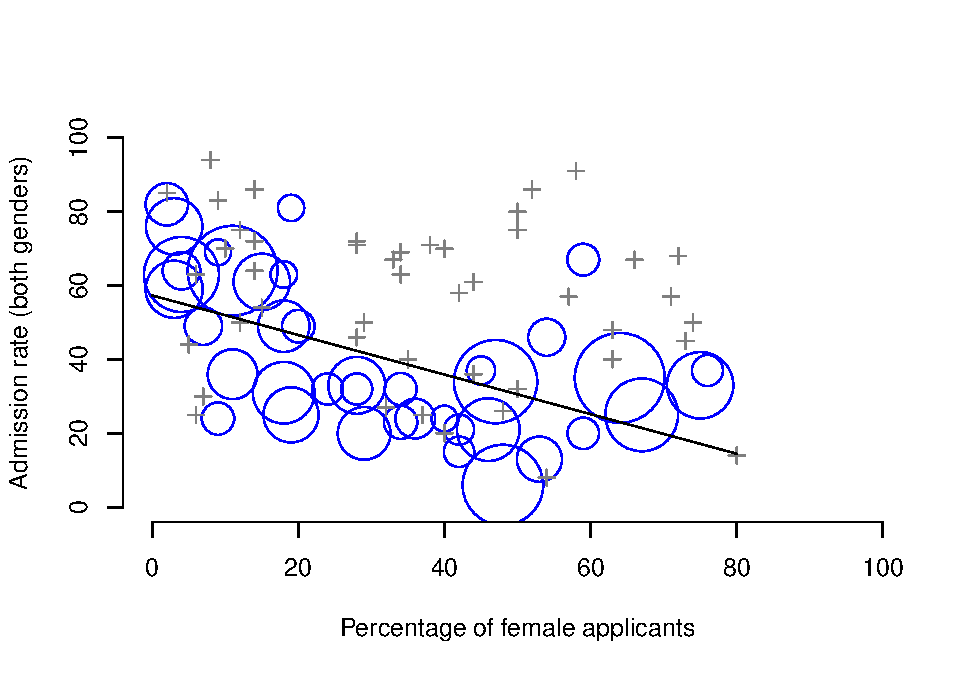
\includegraphics{schuster-statistics-remix_files/figure-latex/berkeley-1.pdf}
\caption{\label{fig:berkeley}The Berkeley 1973 college admissions data. This figure plots the admission rate for the 85 departments that had at least one female applicant, as a function of the percentage of applicants that were female. The plot is a redrawing of Figure 1 from \citet{Bickel1975}. Circles plot departments with more than 40 applicants; the area of the circle is proportional to the total number of applicants. The crosses plot department with fewer than 40 applicants.}
\end{figure}

Before leaving this topic entirely, I want to point out something else really critical that is often overlooked in a research methods class. Statistics only solves \emph{part} of the problem. Remember that we started all this with the concern that Berkeley's admissions processes might be unfairly biased against female applicants. When we looked at the ``aggregated'' data, it did seem like the university was discriminating against women, but when we ``disaggregate'' and looked at the individual behaviour of all the departments, it turned out that the actual departments were, if anything, slightly biased in favour of women. The gender bias in total admissions was caused by the fact that women tended to self-select for harder departments. From a legal perspective, that would probably put the university in the clear. Postgraduate admissions are determined at the level of the individual department (and there are good reasons to do that), and at the level of individual departments, the decisions are more or less unbiased (the weak bias in favour of females at that level is small, and not consistent across departments). Since the university can't dictate which departments people choose to apply to, and the decision making takes place at the level of the department it can hardly be held accountable for any biases that those choices produce.

That was the basis for my somewhat glib remarks earlier, but that's not exactly the whole story, is it? After all, if we're interested in this from a more sociological and psychological perspective, we might want to ask \emph{why} there are such strong gender differences in applications. Why do males tend to apply to engineering more often than females, and why is this reversed for the English department? And why is it it the case that the departments that tend to have a female-application bias tend to have lower overall admission rates than those departments that have a male-application bias? Might this not still reflect a gender bias, even though every single department is itself unbiased? It might. Suppose, hypothetically, that males preferred to apply to ``hard sciences'' and females prefer ``humanities''. And suppose further that the reason for why the humanities departments have low admission rates is because the government doesn't want to fund the humanities (Ph.D.~places, for instance, are often tied to government funded research projects). Does that constitute a gender bias? Or just an unenlightened view of the value of the humanities? What if someone at a high level in the government cut the humanities funds because they felt that the humanities are ``useless chick stuff''. That seems pretty \emph{blatantly} gender biased. None of this falls within the purview of statistics, but it matters to the research project. If you're interested in the overall structural effects of subtle gender biases, then you probably want to look at \emph{both} the aggregated and disaggregated data. If you're interested in the decision making process at Berkeley itself then you're probably only interested in the disaggregated data.

In short there are a lot of critical questions that you can't answer with statistics, but the answers to those questions will have a huge impact on how you analyse and interpret data. And this is the reason why you should always think of statistics as a \emph{tool} to help you learn about your data, no more and no less. It's a powerful tool to that end, but there's no substitute for careful thought.

\hypertarget{studydesign}{%
\section{A brief introduction to research design}\label{studydesign}}

Text by \citet{Navarro2018}

\begin{quote}
\emph{To consult the statistician after an experiment is finished is often merely to ask him to conduct a post mortem examination. He can perhaps say what the experiment died of.}

-- Sir Ronald Fisher\footnote{Presidential Address to the First Indian Statistical Congress, 1938. Source: \url{http://en.wikiquote.org/wiki/Ronald_Fisher}}
\end{quote}

Note that this section is ``special'' in two ways. Firstly, it's much more psychology-specific than the later chapters. Secondly, it focuses much more heavily on the scientific problem of research methodology, and much less on the statistical problem of data analysis. Nevertheless, the two problems are related to one another, so it's traditional for stats textbooks to discuss the problem in a little detail. This chapter relies heavily on \citet{Campbell1963} for the discussion of study design, and \citet{Stevens1946} for the discussion of scales of measurement. Later versions will attempt to be more precise in the citations.

\hypertarget{some-thoughts-about-psychological-measurement}{%
\subsection{Some thoughts about psychological measurement}\label{some-thoughts-about-psychological-measurement}}

Measurement itself is a subtle concept, but basically it comes down to finding some way of assigning numbers, or labels, or some other kind of well-defined descriptions to ``stuff''. So, any of the following would count as a psychological measurement:

\begin{itemize}
\tightlist
\item
  My \textbf{age} is \emph{33 years}.
\item
  I \emph{do not} \textbf{like anchovies}.
\item
  My \textbf{chromosomal gender} is \emph{male}.
\item
  My \textbf{self-identified gender} is \emph{male}.\footnote{Well\ldots{} now this is awkward, isn't it? This section is one of the oldest parts of the book, and it's outdated in a rather embarrassing way. I wrote this in 2010, at which point all of those facts \emph{were} true. Revisiting this in 2018\ldots{} well I'm not 33 any more, but that's not surprising I suppose. I can't imagine my chromosomes have changed, so I'm going to guess my karyotype was then and is now XY. The self-identified gender, on the other hand\ldots{} ah. I suppose the fact that the title page now refers to me as Danielle rather than Daniel might possibly be a giveaway, but I don't typically identify as ``male'' on a gender questionnaire these days, and I prefer \emph{``she/her''} pronouns as a default (it's a long story)! I did think a little about how I was going to handle this in the book, actually. The book has a somewhat distinct authorial voice to it, and I feel like it would be a rather different work if I went back and wrote everything as Danielle and updated all the pronouns in the work. Besides, it would be a lot of work, so I've left my name as ``Dan'' throughout the book, and in ant case ``Dan'' is a perfectly good nickname for ``Danielle'', don't you think? In any case, it's not a big deal. I only wanted to mention it to make life a little easier for readers who aren't sure how to refer to me. I still don't like anchovies though :-)}
\end{itemize}

In the short list above, the \textbf{bolded part} is ``the thing to be measured'', and the \emph{italicised part} is ``the measurement itself''. In fact, we can expand on this a little bit, by thinking about the set of possible measurements that could have arisen in each case:

\begin{itemize}
\tightlist
\item
  My \textbf{age} (in years) could have been \emph{0, 1, 2, 3 \ldots{}}, etc. The upper bound on what my age could possibly be is a bit fuzzy, but in practice you'd be safe in saying that the largest possible age is \emph{150}, since no human has ever lived that long.
\item
  When asked if I \textbf{like anchovies}, I might have said that \emph{I do}, or \emph{I do not}, or \emph{I have no opinion}, or \emph{I sometimes do}.
\item
  My \textbf{chromosomal gender} is almost certainly going to be \emph{male (XY)} or \emph{female (XX)}, but there are a few other possibilities. I could also have \emph{Klinfelter's syndrome (XXY)}, which is more similar to male than to female. And I imagine there are other possibilities too.
\item
  My \textbf{self-identified gender} is also very likely to be \emph{male} or \emph{female}, but it doesn't have to agree with my chromosomal gender. I may also choose to identify with \emph{neither}, or to explicitly call myself \emph{transgender}.
\end{itemize}

As you can see, for some things (like age) it seems fairly obvious what the set of possible measurements should be, whereas for other things it gets a bit tricky. But I want to point out that even in the case of someone's age, it's much more subtle than this. For instance, in the example above, I assumed that it was okay to measure age in years. But if you're a developmental psychologist, that's way too crude, and so you often measure age in \emph{years and months} (if a child is 2 years and 11 months, this is usually written as ``2;11''). If you're interested in newborns, you might want to measure age in \emph{days since birth}, maybe even \emph{hours since birth}. In other words, the way in which you specify the allowable measurement values is important.

Looking at this a bit more closely, you might also realise that the concept of ``age'' isn't actually all that precise. In general, when we say ``age'' we implicitly mean ``the length of time since birth''. But that's not always the right way to do it. Suppose you're interested in how newborn babies control their eye movements. If you're interested in kids that young, you might also start to worry that ``birth'' is not the only meaningful point in time to care about. If Baby Alice is born 3 weeks premature and Baby Bianca is born 1 week late, would it really make sense to say that they are the ``same age'' if we encountered them ``2 hours after birth''? In one sense, yes: by social convention, we use birth as our reference point for talking about age in everyday life, since it defines the amount of time the person has been operating as an independent entity in the world, but from a scientific perspective that's not the only thing we care about. When we think about the biology of human beings, it's often useful to think of ourselves as organisms that have been growing and maturing since conception, and from that perspective Alice and Bianca aren't the same age at all. So you might want to define the concept of ``age'' in two different ways: the length of time since conception, and the length of time since birth. When dealing with adults, it won't make much difference, but when dealing with newborns it might.

Moving beyond these issues, there's the question of methodology. What specific ``measurement method'' are you going to use to find out someone's age? As before, there are lots of different possibilities:

\begin{itemize}
\tightlist
\item
  You could just ask people ``how old are you?'' The method of self-report is fast, cheap and easy, but it only works with people old enough to understand the question, and some people lie about their age.
\item
  You could ask an authority (e.g., a parent) ``how old is your child?'' This method is fast, and when dealing with kids it's not all that hard since the parent is almost always around. It doesn't work as well if you want to know ``age since conception'', since a lot of parents can't say for sure when conception took place. For that, you might need a different authority (e.g., an obstetrician).
\item
  You could look up official records, like birth certificates. This is time consuming and annoying, but it has its uses (e.g., if the person is now dead).
\end{itemize}

\hypertarget{operationalisation-defining-your-measurement}{%
\subsection{Operationalisation: defining your measurement}\label{operationalisation-defining-your-measurement}}

\href{https://youtu.be/p1zqoSSIpsg}{Video: Operationalization}

All of the ideas discussed in the previous section all relate to the concept of \textbf{\emph{operationalisation}}. To be a bit more precise about the idea, operationalisation is the process by which we take a meaningful but somewhat vague concept, and turn it into a precise measurement. The process of operationalisation can involve several different things:

\begin{itemize}
\tightlist
\item
  Being precise about what you are trying to measure. For instance, does ``age'' mean ``time since birth'' or ``time since conception'' in the context of your research?
\item
  Determining what method you will use to measure it. Will you use self-report to measure age, ask a parent, or look up an official record? If you're using self-report, how will you phrase the question?
\item
  Defining the set of the allowable values that the measurement can take. Note that these values don't always have to be numerical, though they often are. When measuring age, the values are numerical, but we still need to think carefully about what numbers are allowed. Do we want age in years, years and months, days, hours? Etc. For other types of measurements (e.g., gender), the values aren't numerical. But, just as before, we need to think about what values are allowed. If we're asking people to self-report their gender, what options to we allow them to choose between? Is it enough to allow only ``male'' or ``female''? Do you need an ``other'' option? Or should we not give people any specific options, and let them answer in their own words? And if you open up the set of possible values to include all verbal response, how will you interpret their answers?
\end{itemize}

Operationalisation is a tricky business, and there's no ``one, true way'' to do it. The way in which you choose to operationalise the informal concept of ``age'' or ``gender'' into a formal measurement depends on what you need to use the measurement for. Often you'll find that the community of scientists who work in your area have some fairly well-established ideas for how to go about it. In other words, operationalisation needs to be thought through on a case by case basis. Nevertheless, while there a lot of issues that are specific to each individual research project, there are some aspects to it that are pretty general.

Before moving on, I want to take a moment to clear up our terminology, and in the process introduce one more term. Here are four different things that are closely related to each other:

\begin{itemize}
\tightlist
\item
  \textbf{\emph{A theoretical construct}}. This is the thing that you're trying to take a measurement of, like ``age'', ``gender'' or an ``opinion''. A theoretical construct can't be directly observed, and often they're actually a bit vague.
\item
  \textbf{\emph{A measure}}. The measure refers to the method or the tool that you use to make your observations. A question in a survey, a behavioural observation or a brain scan could all count as a measure.
\item
  \textbf{\emph{An operationalisation}}. The term ``operationalisation'' refers to the logical connection between the measure and the theoretical construct, or to the process by which we try to derive a measure from a theoretical construct.
\item
  \textbf{\emph{A variable}}. Finally, a new term. A variable is what we end up with when we apply our measure to something in the world. That is, variables are the actual ``data'' that we end up with in our data sets.
\end{itemize}

In practice, even scientists tend to blur the distinction between these things, but it's very helpful to try to understand the differences.

\hypertarget{ivdv}{%
\subsection{The ``role'' of variables: predictors and outcomes}\label{ivdv}}

Okay, I've got one last piece of terminology that I need to explain to you before moving away from variables. Normally, when we do some research we end up with lots of different variables. Then, when we analyse our data we usually try to explain some of the variables in terms of some of the other variables. It's important to keep the two roles ``thing doing the explaining'' and ``thing being explained'' distinct. So let's be clear about this now. Firstly, we might as well get used to the idea of using mathematical symbols to describe variables, since it's going to happen over and over again. Let's denote the ``to be explained'' variable \(Y\), and denote the variables ``doing the explaining'' as \(X_1\), \(X_2\), etc.

Now, when we doing an analysis, we have different names for \(X\) and \(Y\), since they play different roles in the analysis. The classical names for these roles are \textbf{\emph{independent variable}} (IV) and \textbf{\emph{dependent variable}} (DV). The IV is the variable that you use to do the explaining (i.e., \(X\)) and the DV is the variable being explained (i.e., \(Y\)). The logic behind these names goes like this: if there really is a relationship between \(X\) and \(Y\) then we can say that \(Y\) depends on \(X\), and if we have designed our study ``properly'' then \(X\) isn't dependent on anything else. However, I personally find those names horrible: they're hard to remember and they're highly misleading, because (a) the IV is never actually ``independent of everything else'' and (b) if there's no relationship, then the DV doesn't actually depend on the IV. And in fact, because I'm not the only person who thinks that IV and DV are just awful names, there are a number of alternatives that I find more appealing. The terms that I'll use in these notes are \textbf{\emph{predictors}} and \textbf{\emph{outcomes}}. The idea here is that what you're trying to do is use \(X\) (the predictors) to make guesses about \(Y\) (the outcomes).\footnote{Annoyingly, though, there's a lot of different names used out there. I won't list all of them -- there would be no point in doing that -- other than to note that R often uses ``response variable'' where I've used ``outcome'', and a traditionalist would use ``dependent variable''. Sigh. This sort of terminological confusion is very common, I'm afraid.} This is summarised in Table \ref{tab:ivdv}.

\begin{table}

\caption{\label{tab:ivdv}The terminology used to distinguish between different roles that a variable can play when analysing a data set. Note that this book will tend to avoid the classical terminology in favour of the newer names.}
\centering
\begin{tabular}[t]{lll}
\toprule
role of the variable & classical name & modern name\\
\midrule
to be explained & dependent variable (DV) & outcome\\
to do the explaining & independent variable (IV) & predictor\\
\bottomrule
\end{tabular}
\end{table}

\hypertarget{researchdesigns}{%
\subsection{Experimental and non-experimental research}\label{researchdesigns}}

\href{https://youtu.be/H9uDTWD8R4M}{Video: Experimental, Quasi-, and Non-Experimental Research Designs}

One of the big distinctions that you should be aware of is the distinction between ``experimental research'' and ``non-experimental research''. When we make this distinction, what we're really talking about is the degree of control that the researcher exercises over the people and events in the study.

\hypertarget{experimental-research}{%
\subsubsection{Experimental research}\label{experimental-research}}

The key features of \textbf{\emph{experimental research}} is that the researcher controls all aspects of the study, especially what participants experience during the study. In particular, the researcher manipulates or varies the predictor variables (IVs), and then allows the outcome variable (DV) to vary naturally. The idea here is to deliberately vary the predictors (IVs) to see if they have any causal effects on the outcomes. Moreover, in order to ensure that there's no chance that something other than the predictor variables is causing the outcomes, everything else is kept constant or is in some other way ``balanced'' to ensure that they have no effect on the results. In practice, it's almost impossible to \emph{think} of everything else that might have an influence on the outcome of an experiment, much less keep it constant. The standard solution to this is \textbf{\emph{randomisation}}: that is, we randomly assign people to different groups, and then give each group a different treatment (i.e., assign them different values of the predictor variables). We'll talk more about randomisation later in this course, but for now, it's enough to say that what randomisation does is minimise (but not eliminate) the chances that there are any systematic difference between groups.

Let's consider a very simple, completely unrealistic and grossly unethical example. Suppose you wanted to find out if smoking causes lung cancer. One way to do this would be to find people who smoke and people who don't smoke, and look to see if smokers have a higher rate of lung cancer. This is \emph{not} a proper experiment, since the researcher doesn't have a lot of control over who is and isn't a smoker. And this really matters: for instance, it might be that people who choose to smoke cigarettes also tend to have poor diets, or maybe they tend to work in asbestos mines, or whatever. The point here is that the groups (smokers and non-smokers) actually differ on lots of things, not \emph{just} smoking. So it might be that the higher incidence of lung cancer among smokers is caused by something else, not by smoking per se. In technical terms, these other things (e.g.~diet) are called ``confounds'', and we'll talk about those in just a moment.

In the meantime, let's now consider what a proper experiment might look like. Recall that our concern was that smokers and non-smokers might differ in lots of ways. The solution, as long as you have no ethics, is to \emph{control} who smokes and who doesn't. Specifically, if we randomly divide participants into two groups, and force half of them to become smokers, then it's very unlikely that the groups will differ in any respect other than the fact that half of them smoke. That way, if our smoking group gets cancer at a higher rate than the non-smoking group, then we can feel pretty confident that (a) smoking does cause cancer and (b) we're murderers.

\hypertarget{causality-research-and-statistics}{%
\section{Causality, Research, and Statistics}\label{causality-research-and-statistics}}

Text by David Schuster

\href{https://youtu.be/s9itzrOlnq4}{Video: Causality}

\hypertarget{experimental-quasi-experimental-and-non-experimental-studies}{%
\subsection{Experimental, Quasi-Experimental, and Non-Experimental Studies}\label{experimental-quasi-experimental-and-non-experimental-studies}}

In this section, I would like to add a bit more precision to the general concepts explained by \citet{Navarro2018}.

Research psychology is a process of identifying constructs and describing how they relate to other constructs. We can classify research designs as experiments, quasi-experiments, and non-experiments.

Experiments are the only kind of research that shows causal relationships (that is, that construct A causes a change in construct B). So an experiment could show if smoking causes lung cancer. To do this, experiments need two things (or they are not experiments)

All experiments have a manipulation. This means that the experimenter changes something within the environment of the experiment (called an independent variable) to see if it causes a change in the outcome (called a dependent variable). For our smoking example, a manipulation would be assigning one group of participants to a lifetime of smoking and another group of participants to a lifetime of no smoking.

Experiments require random assignment. The experimenter decides when to vary the levels of the manipulation (change the manipulation) based on random assignment. Random assignment means that every participant has the same chance as being in one condition as another. For our smoking example, random assignment means each participant has a 50\% chance of being in the smoking group.

As may be clear from the smoking example, we cannot always do experiments because of ethical (it would be wrong to assign people to smoke) or practical reasons (you cannot randomly assign people to genders, for example). The solution is a quasi- or non-experimental study.

In summary: experiments are powerful because they uniquely demonstrate causality (causal relationships). However, experiments require a manipulation and random assignment, which are not always possible.

In a quasi-experimental study, there is a manipulation but no random assignment. Whenever participants are assigned to levels of a manipulation non-randomly, the research is quasi-experimental. In a quasi-experimental smoking study, we could ask people if they had smoked before and assign them to smoking or non-smoking groups based on that answer.

In summary: quasi-experiments do not require random assignment, but they do not show casual relationships.

In a non-experimental study, no manipulation is done. If you want to look at the effects of gender on lung cancer, you would simply observe (collect data on) the genders of patients. By only observing, you would not be manipulating gender.

The differences between quasi- and non-experimental studies are sometimes slight (Pedhauzer \& Schmelkin, 1991); if the researcher is manipulating an IV, then the work is quasi-experimental.

In summary: non-experimental studies are observational. Like quasi-experimental studies, they do not show causal relationships.

It's worth repeating that only experiments demonstrate causality. Quasi- and non-experiments can show that a relationship exists but do not say whether one variable causes the other. Any non-causal relationship has three possible explanations:

\begin{enumerate}
\def\labelenumi{\arabic{enumi}.}
\tightlist
\item
  A \(\rightarrow\) B one variable causes another; in an experiment, this is the only explanation
\item
  B \(\leftarrow\) A the relationship is reversed; the first variable is actually the outcome
\item
  C \(\rightarrow\) A; C \(\rightarrow\) B a third variable exists that was not measured in the study; the third variable causes a change in both A and B. There are many `C' variables, potentially.
\end{enumerate}

In a non-experimental smoking study, you could not say whether smoking causes lung cancer or people who are predisposed to lung cancer are more likely to smoke. A third possibility is that a separate, third variable causes both lung cancer and a desire to smoke.

\hypertarget{demonstrating-causality}{%
\subsection{Demonstrating Causality}\label{demonstrating-causality}}

In the 19th century, John Stewart Mill said that we could be satisfied that a relationship is causal if the following three things could be demonstrated:

\begin{enumerate}
\def\labelenumi{\arabic{enumi}.}
\tightlist
\item
  The cause preceded the effect
\item
  The cause was related to the effect
\item
  We can find no plausible alternative explanation for the effect other than the cause
\end{enumerate}

Experiments aim to identify causal relationships by manipulating something, observing the outcome, seeing a relationship, and using various methods to reduce other explanations.

\hypertarget{statistics-and-causality}{%
\subsection{Statistics and Causality}\label{statistics-and-causality}}

Statistics are an important tool for establishing causality, but it's important to know that the choice of statistical technique does not affect the level of causal evidence; demonstrating causality is the job of the research design, not the statistics.

A common misconception arises from the term correlational research design, which people use as a label for quasi-experimental and non-experimental research. It is easy to confuse this term with correlation which is a statistical technique.

Recall that statistics has two branches: Descriptive stats provides tools to summarize variability. Inferential stats provides tools for generalizing samples to populations.

To demonstrate causality, we need to satisfy Mill's second requirement. Inferential statistics can help us do that. Two techniques are particularly useful: correlation (and its statistic r) and the t¬-test (and its statistic, t). Next, we will see how these techniques work.

\hypertarget{validity-and-reliability}{%
\subsection{Validity and Reliability}\label{validity-and-reliability}}

Text by David Schuster

\hypertarget{define-validity-and-reliability}{%
\subsubsection{Define validity and reliability}\label{define-validity-and-reliability}}

Reliability and validity are fundamental to critiquing psychological research and to developing your own high-quality research. There are different types of validity and reliability that are relevant to us, which sometimes confuses people. Because of this, introductory textbooks often present convoluted definitions of these concepts. Fortunately, the real definitions are simple:

Reliability means consistency. Something is reliable if it is consistent. The more consistency, the more reliability.

Validity means truth. Something is valid if it is true. Truth is either-or; there is no such thing as ``more true'' or ``less true.''

In other words, good psychological science requires certain types of consistency and for some of the claims we make to be true. Next, we will look at the specific kinds of reliability and validity that are important for scientists.

\hypertarget{types-of-consistency-types-of-reliability}{%
\subsubsection{Types of consistency = Types of Reliability}\label{types-of-consistency-types-of-reliability}}

\href{https://youtu.be/EatmTWbD4uo}{Reliability}

Here are arguably the three most important types of reliability:

\begin{longtable}[]{@{}
  >{\raggedright\arraybackslash}p{(\columnwidth - 6\tabcolsep) * \real{0.06}}
  >{\raggedright\arraybackslash}p{(\columnwidth - 6\tabcolsep) * \real{0.55}}
  >{\raggedright\arraybackslash}p{(\columnwidth - 6\tabcolsep) * \real{0.23}}
  >{\raggedright\arraybackslash}p{(\columnwidth - 6\tabcolsep) * \real{0.16}}@{}}
\toprule
Type of Reliability & Situation & Definition & How to assess \\
\midrule
\endhead
Test-retest & You administer a measure to a participant, then wait some period of time, and give them the test again. The participant's true score on the measure has not changed (e.g., IQ, personality). & The extent to which a measure is consistent across different administrations & Look for a correlation between the two administrations \\
Interrater & A measure involves two or more raters who record subjective observations (e.g., counting the number of times a participant has a tic, counting the number of times a married couple shows affection) & The extent to which two observers are consistent in their ratings & Look for a correlation between the two raters \\
Internal consistency & You are measuring a construct using several items (e.g., five items all rating your enjoyment of a course) & The extent to which items on a measure are consistent with each other; expected if the items measure the same construct & Cronbach's alpha (.7 is acceptable, .8 is good, and .9 is excellent) \\
\bottomrule
\end{longtable}

\hypertarget{validity-is-a-property-of-inferences}{%
\subsubsection{Validity is a property of inferences}\label{validity-is-a-property-of-inferences}}

\href{https://youtu.be/mxZxGttf6sE}{Video: Validity \& Threats}

Validity is a specific kind of truth. Validity is the truth of an inference, or a claim. In other words, validity is a property of inferences. An inference (a claim) is valid if it is true.

For example, I could claim that the earth is round. Hopefully, it is a claim that you accept as being true. If you agree, then you could label my claim as valid.

Validity in research is frequently misunderstood, which leads to bizarre and confusing definitions of validity. There is no such thing as ``a valid study.'' Only claims about the study are valid or not. There is also no such thing as ``a valid researcher.'' A researcher can make claims. Only the researcher's claims are valid or not. There is also no such thing as ``more valid'' or ``increasing validity.'' Validity is truth of a claim. Either a claim is true, or it is not.

For better or for worse, we usually don't know with 100\% certainty if a claim is true or false (if we did, we wouldn't need the research). Therefore, research methods get very interesting when we listen to other researcher's claims and then debate if we agree with them or not. When we do this, we are evaluating the validity of claims made about the study. Next, let's look at different types of claims (inferences) that are made in research.

\hypertarget{types-of-inferences-in-a-study-types-of-validity}{%
\subsubsection{Types of inferences in a study = Types of validity}\label{types-of-inferences-in-a-study-types-of-validity}}

Here are some of the most important types of validity.

\begin{longtable}[]{@{}
  >{\raggedright\arraybackslash}p{(\columnwidth - 6\tabcolsep) * \real{0.30}}
  >{\raggedright\arraybackslash}p{(\columnwidth - 6\tabcolsep) * \real{0.25}}
  >{\raggedright\arraybackslash}p{(\columnwidth - 6\tabcolsep) * \real{0.19}}
  >{\raggedright\arraybackslash}p{(\columnwidth - 6\tabcolsep) * \real{0.27}}@{}}
\toprule
Type of Validity & Type of Claim & Definition & Example claim \\
\midrule
\endhead
Construct validity & The study operations represent the constructs of interest & The truth of claims that study operations match study constructs & ``The Stanford-Binet was used to measure IQ'' \\
Internal validity & The study IV caused a change in the study DV & The truth of claims that the IV causes changes in the DV & ``The control group reported lower levels of stress than the experimental group, suggesting that the manipulation raised stress.'' \\
External validity & The study results apply to situation X & The truth of claims that the findings will apply as participants/units/variables/settings change. & ``Although data were collected from college students, a similar effect would be expected in working adults.'' \\
Statistical conclusion validity & The statistical analysis was significant or not significant & The truth of claims about the size and direction of the relationship between the IV and the DV. Or, that the statistical results are correct. & ``p \textless{} .05, indicating a significant difference'' \\
\bottomrule
\end{longtable}

Finally, you might encounter these other types of validity, but they are less clearly defined and evaluated:

\begin{itemize}
\tightlist
\item
  Content validity: The truth of claims that a measure adequately samples (includes the important elements of) the domain of interest. For example, if IQ includes both verbal and math ability, an IQ test would need to have both verbal and math items.
\item
  Face validity: The truth of claims that a study operation ``seems like'' the construct. For example, a study about distractions from mobile devices might not support claims of ``seeming real'' if the phone in the study is a paper mockup.
\item
  Criterion validity: The truth of claims that a measure can predict or correlate with some outcome of interest. A personality test as part of a job application would have criterion validity if it predicted applicants' success in the job.
\end{itemize}

\hypertarget{threats-to-validity}{%
\subsubsection{Threats to validity}\label{threats-to-validity}}

Threats to validity are specific reasons why an inference about a study is wrong. They can help us anticipate problems in the design of our own research. The best way to address threats to validity is to change the design of our research. Understanding threats to validity also helps you critique research done by others.

\hypertarget{introR}{%
\chapter{Getting started with R}\label{introR}}

Text by \citet{Navarro2018}

\hypertarget{videos}{%
\section{Videos}\label{videos}}

\href{https://www.youtube.com/watch?v=FIrsOBy5k58}{Video: RStudio for the Total Beginner}

\href{https://youtu.be/PVK092WlC4A}{Video: Jump Start Guide to R}

\href{https://youtu.be/8l43-yHsTP0}{Video: Robot Metaphor for R}

\hypertarget{introduction-1}{%
\section{Introduction}\label{introduction-1}}

\begin{quote}
\emph{Robots are nice to work with.}

--Roger Zelazny\footnote{Source: \emph{Dismal Light} (1968).}
\end{quote}

In this chapter I'll discuss how to get started in R. I'll briefly talk about how to download and install R, but most of the chapter will be focused on getting you started typing R commands. Our goal in this chapter is not to learn any statistical concepts: we're just trying to learn the basics of how R works and get comfortable interacting with the system. To do this, we'll spend a bit of time using R as a simple calculator, since that's the easiest thing to do with R. In doing so, you'll get a bit of a feel for what it's like to work in R. From there I'll introduce some very basic programming ideas: in particular, I'll talk about the idea of defining \emph{variables} to store information, and a few things that you can do with these variables.

However, before going into any of the specifics, it's worth talking a little about why you might want to use R at all. Given that you're reading this, you've probably got your own reasons. However, if those reasons are ``because that's what my stats class uses'', it might be worth explaining a little why your lecturer has chosen to use R for the class. Of course, I don't really know why \emph{other} people choose R, so I'm really talking about why I use it.

\begin{itemize}
\tightlist
\item
  It's sort of obvious, but worth saying anyway: doing your statistics on a computer is faster, easier and more powerful than doing statistics by hand. Computers excel at mindless repetitive tasks, and a lot of statistical calculations are both mindless and repetitive. For most people, the only reason to ever do statistical calculations with pencil and paper is for learning purposes. In my class I do occasionally suggest doing some calculations that way, but the only real value to it is pedagogical. It does help you to get a ``feel'' for statistics to do some calculations yourself, so it's worth doing it once. But only once!
\item
  Doing statistics in a spreadsheet (e.g., Microsoft Excel) is generally a bad idea in the long run. Although many people are likely feel more familiar with them, spreadsheets are very limited in terms of what analyses they allow you do. If you get into the habit of trying to do your real life data analysis using spreadsheets, then you've dug yourself into a very deep hole.
\item
  Avoiding proprietary software is a very good idea. There are a lot of commercial packages out there that you can buy, some of which I like and some of which I don't. They're usually very glossy in their appearance, and generally very powerful (much more powerful than spreadsheets). However, they're also very expensive: usually, the company sells ``student versions'' (limited versions of the real thing) very cheaply; they sell full powered ``educational versions'' at a price that makes me wince; and they sell commercial licences with a staggeringly high price tag. The business model here is to suck you in during your student days, and then leave you dependent on their tools when you go out into the real world. It's hard to blame them for trying, but personally I'm not in favour of shelling out thousands of dollars if I can avoid it. And you can avoid it: if you make use of packages like R that are open source and free, you never get trapped having to pay exorbitant licensing fees.
\item
  Something that you might not appreciate now, but will love later on if you do anything involving data analysis, is the fact that R is highly extensible. When you download and install R, you get all the basic ``packages'', and those are very powerful on their own. However, because R is so open and so widely used, it's become something of a standard tool in statistics, and so lots of people write their own packages that extend the system. And these are freely available too. One of the consequences of this, I've noticed, is that if you open up an advanced textbook (a recent one, that is) rather than introductory textbooks, is that a \emph{lot} of them use R. In other words, if you learn how to do your basic statistics in R, then you're a lot closer to being able to use the state of the art methods than you would be if you'd started out with a ``simpler'' system: so if you want to become a genuine expert in psychological data analysis, learning R is a very good use of your time.
\item
  Related to the previous point: R is a real programming language. As you get better at using R for data analysis, you're also learning to program. To some people this might seem like a bad thing, but in truth, programming is a core research skill across a lot of the social and behavioural sciences. Think about how many surveys and experiments are done online, or presented on computers. Think about all those online social environments which you might be interested in studying; and maybe collecting data from in an automated fashion. Think about artificial intelligence systems, computer vision and speech recognition. If any of these are things that you think you might want to be involved in -- as someone ``doing research in psychology'', that is -- you'll need to know a bit of programming. And if you don't already know how to program, then learning how to do statistics using R is a nice way to start.
\end{itemize}

Those are the main reasons I use R. It's not without its flaws: it's not easy to learn, and it has a few very annoying quirks to it that we're all pretty much stuck with, but on the whole I think the strengths outweigh the weakness; more so than any other option I've encountered so far.

\hypertarget{gettingR}{%
\section{Installing R}\label{gettingR}}

Okay, enough with the sales pitch. Let's get started. Just as with any piece of software, R needs to be installed on a ``computer'', which is a magical box that does cool things and delivers free ponies. Or something along those lines: I may be confusing computers with the iPad marketing campaigns. Anyway, R is freely distributed online, and you can download it from the R homepage, which is:

\begin{quote}
\url{http://cran.r-project.org/}
\end{quote}

At the top of the page -- under the heading ``Download and Install R'' -- you'll see separate links for Windows users, Mac users, and Linux users. If you follow the relevant link, you'll see that the online instructions are pretty self-explanatory, but I'll walk you through the installation anyway. As of this writing, the current version of R is 3.0.2 (``Frisbee Sailing"), but they usually issue updates every six months, so you'll probably have a newer version.\footnote{Although R is updated frequently, it doesn't usually make much of a difference for the sort of work we'll do in this book. In fact, during the writing of the book I upgraded several times, and didn't have to change much except these sections describing the downloading.}

\hypertarget{installing-r-on-a-windows-computer}{%
\subsection{Installing R on a Windows computer}\label{installing-r-on-a-windows-computer}}

The CRAN homepage changes from time to time, and it's not particularly pretty, or all that well-designed quite frankly. But it's not difficult to find what you're after. In general you'll find a link at the top of the page with the text ``Download R for Windows''. If you click on that, it will take you to a page that offers you a few options. Again, at the very top of the page you'll be told to click on a link that says to click here if you're installing R for the first time. That's probably what you want. This will take you to a page that has a prominent link at the top called ``Download R 3.0.2 for Windows''. That's the one you want. Click on that and your browser should start downloading a file called \texttt{R-3.0.2-win.exe}, or whatever the equivalent version number is by the time you read this. The file for version 3.0.2 is about 54MB in size, so it may take some time depending on how fast your internet connection is. Once you've downloaded the file, double click to install it. As with any software you download online, Windows will ask you some questions about whether you trust the file and so on. After you click through those, it'll ask you where you want to install it, and what components you want to install. The default values should be fine for most people, so again, just click through. Once all that is done, you should have R installed on your system. You can access it from the Start menu, or from the desktop if you asked it to add a shortcut there. You can now open up R in the usual way if you want to, but what I'm going to suggest is that instead of doing that you should now install RStudio (see Section \ref{installingrstudio} for instructions).

\hypertarget{installing-r-on-a-mac}{%
\subsection{Installing R on a Mac}\label{installing-r-on-a-mac}}

When you click on the Mac OS X link, you should find yourself on a page with the title ``R for Mac OS X''. The vast majority of Mac users will have a fairly recent version of the operating system: as long as you're running Mac OS X 10.6 (Snow Leopard) or higher, then you'll be fine.\footnote{If you're running an older version of the Mac OS, then you need to follow the link to the ``old'' page (\url{http://cran.r-project.org/bin/macosx/old/}). You should be able to find the installer file that you need at the bottom of the page.} There's a fairly prominent link on the page called ``R-3.0.2.pkg'', which is the one you want. Click on that link and you'll start downloading the installer file, which is (not surprisingly) called \texttt{R-3.0.2.pkg}. It's about 61MB in size, so the download can take a while on slower internet connections.

Once you've downloaded \texttt{R-3.0.2.pkg}, all you need to do is open it by double clicking on the package file. The installation should go smoothly from there: just follow all the instructions just like you usually do when you install something. Once it's finished, you'll find a file called \texttt{R.app} in the Applications folder. You can now open up R in the usual way\footnote{Tip for advanced Mac users. You can run R from the terminal if you want to. The command is just ``R''. It behaves like the normal desktop version, except that help documentation behaves like a ``man'' page instead of opening in a new window.} if you want to, but what I'm going to suggest is that instead of doing that you should now install RStudio (see Section \ref{installingrstudio} for instructions).

\hypertarget{installing-r-on-a-linux-computer}{%
\subsection{Installing R on a Linux computer}\label{installing-r-on-a-linux-computer}}

If you're successfully managing to run a Linux box, regardless of what distribution, then you should find the instructions on the website easy enough. You can compile R from source yourself if you want, or install it through your package management system, which will probably have R in it.
Alternatively, the CRAN site has precompiled binaries for Debian, Red Hat, Suse and Ubuntu and has separate instructions for each. Once you've got R installed, you can run it from the command line just by typing \texttt{R}. However, if you're feeling envious of Windows and Mac users for their fancy GUIs, you can download RStudio too (see Section \ref{installingrstudio} for instructions).

\hypertarget{installingrstudio}{%
\subsection{Downloading and installing RStudio}\label{installingrstudio}}

Okay, so regardless of what operating system you're using, the last thing that I told you to do is to download RStudio. To understand why I've suggested this, you need to understand a little bit more about R itself. The term R doesn't really refer to a specific application on your computer. Rather, it refers to the underlying statistical language. You can use this language through lots of different applications. When you install R initially, it comes with one application that lets you do this: it's the R.exe application on a Windows machine, and the R.app application on a Mac. But that's not the only way to do it. There are lots of different applications that you can use that will let you interact with R. One of those is called RStudio, and it's the one I'm going to suggest that you use. RStudio provides a clean, professional interface to R that I find much nicer to work with than either the Windows or Mac defaults. Like R itself, RStudio is free software: you can find all the details on their webpage. In the meantime, you can download it here:

\begin{quote}
\url{http://www.RStudio.org/}
\end{quote}

When you visit the RStudio website, you'll probably be struck by how much cleaner and simpler it is than the CRAN website,\footnote{This is probably no coincidence: the people who design and distribute the core R language itself are focused on technical stuff. And sometimes they almost seem to forget that there's an actual human user at the end. The people who design and distribute RStudio are focused on user interface. They want to make R as usable as possible. The two websites reflect that difference.} and how obvious it is what you need to do: click the big green button that says ``Download''.

When you click on the download button on the homepage it will ask you to choose whether you want the desktop version or the server version. You want the desktop version. After choosing the desktop version it will take you to a page \url{http://www.RStudio.org/download/desktop}) that shows several possible downloads: there's a different one for each operating system. However, the nice people at RStudio have designed the webpage so that it automatically recommends the download that is most appropriate for your computer. Click on the appropriate link, and the RStudio installer file will start downloading.

Once it's finished downloading, open the installer file in the usual way to install RStudio. After it's finished installing, you can start R by opening RStudio. You don't need to open R.app or R.exe in order to access R. RStudio will take care of that for you. To illustrate what RStudio looks like, Figure \ref{fig:RStudio} shows a screenshot of an R session in progress. In this screenshot, you can see that it's running on a Mac, but it looks almost identical no matter what operating system you have. The Windows version looks more like a Windows application (e.g., the menus are attached to the application window and the colour scheme is slightly different), but it's more or less identical. There are a few minor differences in where things are located in the menus (I'll point them out as we go along) and in the shortcut keys, because RStudio is trying to ``feel'' like a proper Mac application or a proper Windows application, and this means that it has to change its behaviour a little bit depending on what computer it's running on. Even so, these differences are very small: I started out using the Mac version of RStudio and then started using the Windows version as well in order to write these notes.

\begin{figure}
\includegraphics[width=24.47in]{/Users/dave/Documents/GitHub/stats-remix-advanced/bookdown/img/introR/RStudio2} \caption{An R session in progress running through RStudio. The picture shows RStudio running on a Mac, but the Windows interface is almost identical.}\label{fig:RStudio}
\end{figure}

The only ``shortcoming'' I've found with RStudio is that -- as of this writing -- it's still a work in progress. The ``problem'' is that they keep improving it. New features keep turning up the more recent releases, so there's a good chance that by the time you read this book there will be a version out that has some really neat things that weren't in the version that I'm using now.

\hypertarget{startingR}{%
\subsection{Starting up R}\label{startingR}}

One way or another, regardless of what operating system you're using and regardless of whether you're using RStudio, or the default GUI, or even the command line, it's time to open R and get started. When you do that, the first thing you'll see (assuming that you're looking at the \textbf{\emph{R console}}, that is) is a whole lot of text that doesn't make much sense. It should look something like this:

\begin{verbatim}
R version 3.0.2 (2013-09-25) -- "Frisbee Sailing"
Copyright (C) 2013 The R Foundation for Statistical Computing
Platform: x86_64-apple-darwin10.8.0 (64-bit)

R is free software and comes with ABSOLUTELY NO WARRANTY.
You are welcome to redistribute it under certain conditions.
Type 'license()' or 'licence()' for distribution details.

  Natural language support but running in an English locale

R is a collaborative project with many contributors.
Type 'contributors()' for more information and
'citation()' on how to cite R or R packages in publications.

Type 'demo()' for some demos, 'help()' for on-line help, or
'help.start()' for an HTML browser interface to help.
Type 'q()' to quit R.

> 
\end{verbatim}

Most of this text is pretty uninteresting, and when doing real data analysis you'll never really pay much attention to it. The important part of it is this\ldots{}

\begin{verbatim}
>
\end{verbatim}

\ldots{} which has a flashing cursor next to it. That's the \textbf{\emph{command prompt}}. When you see this, it means that R is waiting patiently for you to do something!

\hypertarget{firstcommand}{%
\section{Typing commands at the R console}\label{firstcommand}}

\textbf{See also: video links at the start of this chapter}

One of the easiest things you can do with R is use it as a simple calculator, so it's a good place to start. For instance, try typing \texttt{10\ +\ 20}, and hitting enter.\footnote{Seriously. If you're in a position to do so, open up R and start typing. The simple act of typing it rather than ``just reading'' makes a big difference. It makes the concepts more concrete, and it ties the abstract ideas (programming and statistics) to the actual context in which you need to use them. Statistics is something you \emph{do}, not just something you read about in a textbook.} When you do this, you've entered a \textbf{\emph{command}}, and R will ``execute'' that command. What you see on screen now will be this:

\begin{Shaded}
\begin{Highlighting}[]
\SpecialCharTok{\textgreater{}} \DecValTok{10} \SpecialCharTok{+} \DecValTok{20}
\NormalTok{[}\DecValTok{1}\NormalTok{] }\DecValTok{30}
\end{Highlighting}
\end{Shaded}

Not a lot of surprises in this extract. But there's a few things worth talking about, even with such a simple example. Firstly, it's important that you understand how to read the extract. In this example, what \emph{I} typed was the \texttt{10\ +\ 20} part. I didn't type the \texttt{\textgreater{}} symbol: that's just the R command prompt and isn't part of the actual command. And neither did I type the \texttt{{[}1{]}\ 30} part. That's what R printed out in response to my command.

Secondly, it's important to understand how the output is formatted. Obviously, the correct answer to the sum \texttt{10\ +\ 20} is \texttt{30}, and not surprisingly R has printed that out as part of its response. But it's also printed out this \texttt{{[}1{]}} part, which probably doesn't make a lot of sense to you right now. You're going to see that a lot. I'll talk about what this means in a bit more detail later on, but for now you can think of \texttt{{[}1{]}\ 30} as if R were saying ``the answer to the 1st question you asked is 30''. That's not quite the truth, but it's close enough for now. And in any case it's not really very interesting at the moment: we only asked R to calculate one thing, so obviously there's only one answer printed on the screen. Later on this will change, and the \texttt{{[}1{]}} part will start to make a bit more sense. For now, I just don't want you to get confused or concerned by it.

\hypertarget{an-important-digression-about-formatting}{%
\subsection{An important digression about formatting}\label{an-important-digression-about-formatting}}

Now that I've taught you these rules I'm going to change them pretty much immediately. That is because I want you to be able to copy code from the book directly into R if if you want to test things or conduct your own analyses. However, if you copy this kind of code (that shows the command prompt and the results) directly into R you will get an error

\begin{Shaded}
\begin{Highlighting}[]
\SpecialCharTok{\textgreater{}} \DecValTok{10} \SpecialCharTok{+} \DecValTok{20}
\NormalTok{[}\DecValTok{1}\NormalTok{] }\DecValTok{30}
\end{Highlighting}
\end{Shaded}

\begin{verbatim}
## Error: <text>:1:1: unexpected '>'
## 1: >
##     ^
\end{verbatim}

So instead, I'm going to provide code in a slightly different format so that it looks like this\ldots{}

\begin{Shaded}
\begin{Highlighting}[]
\DecValTok{10} \SpecialCharTok{+} \DecValTok{20}
\end{Highlighting}
\end{Shaded}

\begin{verbatim}
## [1] 30
\end{verbatim}

There are two main differences.

\begin{itemize}
\tightlist
\item
  In your console, you type after the \textgreater, but from now I I won't show the command prompt in the book.\\
\item
  In the book, output is commented out with \#\#, in your console it appears directly after your code.
\end{itemize}

These two differences mean that if you're working with an electronic version of the book, you can easily copy code out of the book and into the console.

So for example if you copied the two lines of code from the book you'd get this

\begin{Shaded}
\begin{Highlighting}[]
\DecValTok{10} \SpecialCharTok{+} \DecValTok{20}
\end{Highlighting}
\end{Shaded}

\begin{verbatim}
## [1] 30
\end{verbatim}

\begin{Shaded}
\begin{Highlighting}[]
\DocumentationTok{\#\# [1] 30}
\end{Highlighting}
\end{Shaded}

\hypertarget{be-very-careful-to-avoid-typos}{%
\subsection{Be very careful to avoid typos}\label{be-very-careful-to-avoid-typos}}

Before we go on to talk about other types of calculations that we can do with R, there's a few other things I want to point out. The first thing is that, while R is good software, it's still software. It's pretty stupid, and because it's stupid it can't handle typos. It takes it on faith that you meant to type \emph{exactly} what you did type. For example, suppose that you forgot to hit the shift key when trying to type \texttt{+}, and as a result your command ended up being \texttt{10\ =\ 20} rather than \texttt{10\ +\ 20}. Here's what happens:

\begin{Shaded}
\begin{Highlighting}[]
\DecValTok{10} \OtherTok{=} \DecValTok{20}
\end{Highlighting}
\end{Shaded}

\begin{verbatim}
## Error in 10 = 20: invalid (do_set) left-hand side to assignment
\end{verbatim}

What's happened here is that R has attempted to interpret \texttt{10\ =\ 20} as a command, and spits out an error message because the command doesn't make any sense to it. When a \emph{human} looks at this, and then looks down at his or her keyboard and sees that \texttt{+} and \texttt{=} are on the same key, it's pretty obvious that the command was a typo. But R doesn't know this, so it gets upset. And, if you look at it from its perspective, this makes sense. All that R ``knows'' is that \texttt{10} is a legitimate number, \texttt{20} is a legitimate number, and \texttt{=} is a legitimate part of the language too. In other words, from its perspective this really does look like the user meant to type \texttt{10\ =\ 20}, since all the individual parts of that statement are legitimate and it's too stupid to realise that this is probably a typo. Therefore, R takes it on faith that this is exactly what you meant\ldots{} it only ``discovers'' that the command is nonsense when it tries to follow your instructions, typo and all. And then it whinges, and spits out an error.

Even more subtle is the fact that some typos won't produce errors at all, because they happen to correspond to ``well-formed'' R commands. For instance, suppose that not only did I forget to hit the shift key when trying to type \texttt{10\ +\ 20}, I also managed to press the key next to one I meant do. The resulting typo would produce the command \texttt{10\ -\ 20}. Clearly, R has no way of knowing that you meant to \emph{add} 20 to 10, not \emph{subtract} 20 from 10, so what happens this time is this:

\begin{Shaded}
\begin{Highlighting}[]
\DecValTok{10} \SpecialCharTok{{-}} \DecValTok{20}
\end{Highlighting}
\end{Shaded}

\begin{verbatim}
## [1] -10
\end{verbatim}

In this case, R produces the right answer, but to the the wrong question.

To some extent, I'm stating the obvious here, but it's important. The people who wrote R are smart. You, the user, are smart. But R itself is dumb. And because it's dumb, it has to be mindlessly obedient. It does \emph{exactly} what you ask it to do. There is no equivalent to ``autocorrect'' in R, and for good reason. When doing advanced stuff -- and even the simplest of statistics is pretty advanced in a lot of ways -- it's dangerous to let a mindless automaton like R try to overrule the human user. But because of this, it's your responsibility to be careful. Always make sure you type \emph{exactly what you mean}. When dealing with computers, it's not enough to type ``approximately'' the right thing. In general, you absolutely \emph{must} be precise in what you say to R \ldots{} like all machines it is too stupid to be anything other than absurdly literal in its interpretation.

\hypertarget{r-is-a-bit-flexible-with-spacing}{%
\subsection{R is (a bit) flexible with spacing}\label{r-is-a-bit-flexible-with-spacing}}

Of course, now that I've been so uptight about the importance of always being precise, I should point out that there are some exceptions. Or, more accurately, there are some situations in which R does show a bit more flexibility than my previous description suggests. The first thing R is smart enough to do is ignore redundant spacing. What I mean by this is that, when I typed \texttt{10\ +\ 20} before, I could equally have done this

\begin{Shaded}
\begin{Highlighting}[]
\DecValTok{10}    \SpecialCharTok{+} \DecValTok{20}
\end{Highlighting}
\end{Shaded}

\begin{verbatim}
## [1] 30
\end{verbatim}

or this

\begin{Shaded}
\begin{Highlighting}[]
\DecValTok{10}\SpecialCharTok{+}\DecValTok{20}
\end{Highlighting}
\end{Shaded}

\begin{verbatim}
## [1] 30
\end{verbatim}

and I would get exactly the same answer. However, that doesn't mean that you can insert spaces in any old place. When we looked at the startup documentation in Section \ref{startingR} it suggested that you could type \texttt{citation()} to get some information about how to cite R. If I do so\ldots{}

\begin{Shaded}
\begin{Highlighting}[]
\FunctionTok{citation}\NormalTok{()}
\end{Highlighting}
\end{Shaded}

\begin{verbatim}
## 
## To cite R in publications use:
## 
##   R Core Team (2020). R: A language and environment for statistical
##   computing. R Foundation for Statistical Computing, Vienna, Austria.
##   URL https://www.R-project.org/.
## 
## A BibTeX entry for LaTeX users is
## 
##   @Manual{,
##     title = {R: A Language and Environment for Statistical Computing},
##     author = {{R Core Team}},
##     organization = {R Foundation for Statistical Computing},
##     address = {Vienna, Austria},
##     year = {2020},
##     url = {https://www.R-project.org/},
##   }
## 
## We have invested a lot of time and effort in creating R, please cite it
## when using it for data analysis. See also 'citation("pkgname")' for
## citing R packages.
\end{verbatim}

\ldots{} it tells me to cite the R manual \citep{R2013}. Let's see what happens when I try changing the spacing. If I insert spaces in between the word and the parentheses, or inside the parentheses themselves, then all is well. That is, either of these two commands

\begin{Shaded}
\begin{Highlighting}[]
\FunctionTok{citation}\NormalTok{ ()}
\end{Highlighting}
\end{Shaded}

\begin{Shaded}
\begin{Highlighting}[]
\FunctionTok{citation}\NormalTok{(  )}
\end{Highlighting}
\end{Shaded}

will produce exactly the same response. However, what I can't do is insert spaces in the middle of the word. If I try to do this, R gets upset:

\begin{Shaded}
\begin{Highlighting}[]
\NormalTok{citat }\FunctionTok{ion}\NormalTok{()}
\end{Highlighting}
\end{Shaded}

\begin{verbatim}
## Error: <text>:1:7: unexpected symbol
## 1: citat ion
##           ^
\end{verbatim}

Throughout this book I'll vary the way I use spacing a little bit, just to give you a feel for the different ways in which spacing can be used. I'll try not to do it too much though, since it's generally considered to be good practice to be consistent in how you format your commands.

\hypertarget{r-can-sometimes-tell-that-youre-not-finished-yet-but-not-often}{%
\subsection{R can sometimes tell that you're not finished yet (but not often)}\label{r-can-sometimes-tell-that-youre-not-finished-yet-but-not-often}}

One more thing I should point out. If you hit enter in a situation where it's ``obvious'' to R that you haven't actually finished typing the command, R is just smart enough to keep waiting. For example, if you type \texttt{10\ +} and then press enter, even R is smart enough to realise that you probably wanted to type in another number. So here's what happens (for illustrative purposes I'm breaking my own code formatting rules in this section):

\begin{verbatim}
> 10+
+ 
\end{verbatim}

and there's a blinking cursor next to the plus sign. What this means is that R is still waiting for you to finish. It ``thinks'' you're still typing your command, so it hasn't tried to execute it yet. In other words, this plus sign is actually another command prompt. It's different from the usual one (i.e., the \texttt{\textgreater{}} symbol) to remind you that R is going to ``add'' whatever you type now to what you typed last time. For example, if I then go on to type \texttt{3} and hit enter, what I get is this:

\begin{verbatim}
> 10 +
+ 20
[1] 30
\end{verbatim}

And as far as R is concerned, this is \emph{exactly} the same as if you had typed \texttt{10\ +\ 20}. Similarly, consider the \texttt{citation()} command that we talked about in the previous section. Suppose you hit enter after typing \texttt{citation(}. Once again, R is smart enough to realise that there must be more coming -- since you need to add the \texttt{)} character -- so it waits. I can even hit enter several times and it will keep waiting:

\begin{verbatim}
> citation(
+ 
+ 
+ )
\end{verbatim}

I'll make use of this a lot in this book. A lot of the commands that we'll have to type are pretty long, and they're visually a bit easier to read if I break it up over several lines. If you start doing this yourself, you'll eventually get yourself in trouble (it happens to us all). Maybe you start typing a command, and then you realise you've screwed up. For example,

\begin{verbatim}
> citblation( 
+ 
+ 
\end{verbatim}

You'd probably prefer R not to try running this command, right? If you want to get out of this situation, just hit the `escape' key.\footnote{If you're running R from the terminal rather than from RStudio, escape doesn't work: use CTRL-C instead.} R will return you to the normal command prompt (i.e.~\texttt{\textgreater{}}) \emph{without} attempting to execute the botched command.

That being said, it's not often the case that R is smart enough to tell that there's more coming.
For instance, in the same way that I can't add a space in the middle of a word, I can't hit enter in the middle of a word either. If I hit enter after typing \texttt{citat} I get an error, because R thinks I'm interested in an ``object'' called \texttt{citat} and can't find it:

\begin{verbatim}
> citat
Error: object 'citat' not found
\end{verbatim}

What about if I typed \texttt{citation} and hit enter? In this case we get something very odd, something that we definitely \emph{don't} want, at least at this stage. Here's what happens:

\begin{verbatim}
citation
## function (package = "base", lib.loc = NULL, auto = NULL) 
## {
##     dir <- system.file(package = package, lib.loc = lib.loc)
##     if (dir == "") 
##         stop(gettextf("package '%s' not found", package), domain = NA)

BLAH BLAH BLAH
\end{verbatim}

where the \texttt{BLAH\ BLAH\ BLAH} goes on for rather a long time, and you don't know enough R yet to understand what all this gibberish actually means (of course, it doesn't actually say BLAH BLAH BLAH - it says some other things we don't understand or need to know that I've edited for length) This incomprehensible output can be quite intimidating to novice users, and unfortunately it's very easy to forget to type the parentheses; so almost certainly you'll do this by accident. Do not panic when this happens. Simply ignore the gibberish. As you become more experienced this gibberish will start to make sense, and you'll find it quite handy to print this stuff out.\footnote{For advanced users: yes, as you've probably guessed, R is printing out the source code for the function.} But for now just try to remember to add the parentheses when typing your commands.

\hypertarget{arithmetic}{%
\section{Doing simple calculations with R}\label{arithmetic}}

Okay, now that we've discussed some of the tedious details associated with typing R commands, let's get back to learning how to use the most powerful piece of statistical software in the world as a \$2 calculator. So far, all we know how to do is addition. Clearly, a calculator that only did addition would be a bit stupid, so I should tell you about how to perform other simple calculations using R. But first, some more terminology. Addition is an example of an ``operation'' that you can perform (specifically, an arithmetic operation), and the \textbf{\emph{operator}} that performs it is \texttt{+}. To people with a programming or mathematics background, this terminology probably feels pretty natural, but to other people it might feel like I'm trying to make something very simple (addition) sound more complicated than it is (by calling it an arithmetic operation). To some extent, that's true: if addition was the only operation that we were interested in, it'd be a bit silly to introduce all this extra terminology. However, as we go along, we'll start using more and more different kinds of operations, so it's probably a good idea to get the language straight now, while we're still talking about very familiar concepts like addition!

\hypertarget{adding-subtracting-multiplying-and-dividing}{%
\subsection{Adding, subtracting, multiplying and dividing}\label{adding-subtracting-multiplying-and-dividing}}

So, now that we have the terminology, let's learn how to perform some arithmetic operations in R. To that end, Table \ref{tab:arithmetic1} lists the operators that correspond to the basic arithmetic we learned in primary school: addition, subtraction, multiplication and division.

\begin{table}

\caption{\label{tab:arithmetic1}Basic arithmetic operations in R. These five operators are used very frequently throughout the text, so it's important to be familiar with them at the outset.}
\centering
\begin{tabular}[t]{lccc}
\toprule
operation & operator & example input & example output\\
\midrule
addition & `+` & 10 + 2 & 12\\
subtraction & `-` & 9 - 3 & 6\\
multiplication & `*` & 5 * 5 & 25\\
division & `/` & 10 / 3 & 3\\
power & `\textasciicircum{}` & 5 \textasciicircum{} 2 & 25\\
\bottomrule
\end{tabular}
\end{table}

As you can see, R uses fairly standard symbols to denote each of the different operations you might want to perform: addition is done using the \texttt{+} operator, subtraction is performed by the \texttt{-} operator, and so on. So if I wanted to find out what 57 times 61 is (and who wouldn't?), I can use R instead of a calculator, like so:

\begin{Shaded}
\begin{Highlighting}[]
\DecValTok{57} \SpecialCharTok{*} \DecValTok{61}
\end{Highlighting}
\end{Shaded}

\begin{verbatim}
## [1] 3477
\end{verbatim}

So that's handy.

\hypertarget{taking-powers}{%
\subsection{Taking powers}\label{taking-powers}}

The first four operations listed in Table \ref{tab:arithmetic1} are things we all learned in primary school, but they aren't the only arithmetic operations built into R. There are three other arithmetic operations that I should probably mention: taking powers, doing integer division, and calculating a modulus. Of the three, the only one that is of any real importance for the purposes of this book is taking powers, so I'll discuss that one here: the other two are discussed in Chapter \ref{datahandling}.

For those of you who can still remember your high school maths, this should be familiar. But for some people high school maths was a long time ago, and others of us didn't listen very hard in high school. It's not complicated. As I'm sure everyone will probably remember the moment they read this, the act of multiplying a number \(x\) by itself \(n\) times is called ``raising \(x\) to the \(n\)-th power''. Mathematically, this is written as \(x^n\). Some values of \(n\) have special names: in particular \(x^2\) is called \(x\)-squared, and \(x^3\) is called \(x\)-cubed. So, the 4th power of 5 is calculated like this:
\[
5^4 = 5 \times 5 \times 5 \times 5 
\]

One way that we could calculate \(5^4\) in R would be to type in the complete multiplication as it is shown in the equation above. That is, we could do this

\begin{Shaded}
\begin{Highlighting}[]
\DecValTok{5} \SpecialCharTok{*} \DecValTok{5} \SpecialCharTok{*} \DecValTok{5} \SpecialCharTok{*} \DecValTok{5}
\end{Highlighting}
\end{Shaded}

\begin{verbatim}
## [1] 625
\end{verbatim}

but it does seem a bit tedious. It would be very annoying indeed if you wanted to calculate \(5^{15}\), since the command would end up being quite long. Therefore, to make our lives easier, we use the power operator instead. When we do that, our command to calculate \(5^4\) goes like this:

\begin{Shaded}
\begin{Highlighting}[]
\DecValTok{5} \SpecialCharTok{\^{}} \DecValTok{4}
\end{Highlighting}
\end{Shaded}

\begin{verbatim}
## [1] 625
\end{verbatim}

Much easier.

\hypertarget{bedmas}{%
\subsection{Doing calculations in the right order}\label{bedmas}}

Okay. At this point, you know how to take one of the most powerful pieces of statistical software in the world, and use it as a \$2 calculator. And as a bonus, you've learned a few very basic programming concepts. That's not nothing (you could argue that you've just saved yourself \$2) but on the other hand, it's not very much either. In order to use R more effectively, we need to introduce more programming concepts.

In most situations where you would want to use a calculator, you might want to do multiple calculations. R lets you do this, just by typing in longer commands. \footnote{If you're reading this with R open, a good learning trick is to try typing in a few different variations on what I've done here. If you experiment with your commands, you'll quickly learn what works and what doesn't} In fact, we've already seen an example of this earlier, when I typed in \texttt{5\ *\ 5\ *\ 5\ *\ 5}. However, let's try a slightly different example:

\begin{Shaded}
\begin{Highlighting}[]
\DecValTok{1} \SpecialCharTok{+} \DecValTok{2} \SpecialCharTok{*} \DecValTok{4}
\end{Highlighting}
\end{Shaded}

\begin{verbatim}
## [1] 9
\end{verbatim}

Clearly, this isn't a problem for R either. However, it's worth stopping for a second, and thinking about what R just did. Clearly, since it gave us an answer of \texttt{9} it must have multiplied \texttt{2\ *\ 4} (to get an interim answer of 8) and then added 1 to that. But, suppose it had decided to just go from left to right: if R had decided instead to add \texttt{1+2} (to get an interim answer of 3) and then multiplied by 4, it would have come up with an answer of \texttt{12}.

To answer this, you need to know the \textbf{\emph{order of operations}} that R uses. If you remember back to your high school maths classes, it's actually the same order that you got taught when you were at school: the ``\textbf{\emph{BEDMAS}}'' order.\footnote{For advanced users: if you want a table showing the complete order of operator precedence in R, type \texttt{?Syntax}. I haven't included it in this book since there are quite a few different operators, and we don't need that much detail. Besides, in practice most people seem to figure it out from seeing examples: until writing this book I never looked at the formal statement of operator precedence for any language I ever coded in, and never ran into any difficulties.} That is, first calculate things inside \textbf{B}rackets \texttt{()}, then calculate \textbf{E}xponents \texttt{\^{}}, then \textbf{D}ivision \texttt{/} and \textbf{M}ultiplication \texttt{*}, then \textbf{A}ddition \texttt{+} and \textbf{S}ubtraction \texttt{-}. So, to continue the example above, if we want to force R to calculate the \texttt{1+2} part before the multiplication, all we would have to do is enclose it in brackets:

\begin{Shaded}
\begin{Highlighting}[]
\NormalTok{(}\DecValTok{1} \SpecialCharTok{+} \DecValTok{2}\NormalTok{) }\SpecialCharTok{*} \DecValTok{4} 
\end{Highlighting}
\end{Shaded}

\begin{verbatim}
## [1] 12
\end{verbatim}

This is a fairly useful thing to be able to do. The only other thing I should point out about order of operations is what to expect when you have two operations that have the same priority: that is, how does R resolve ties? For instance, multiplication and division are actually the same priority, but what should we expect when we give R a problem like \texttt{4\ /\ 2\ *\ 3} to solve? If it evaluates the multiplication first and then the division, it would calculate a value of two-thirds. But if it evaluates the division first it calculates a value of 6. The answer, in this case, is that R goes from \emph{left to right}, so in this case the division step would come first:

\begin{Shaded}
\begin{Highlighting}[]
\DecValTok{4} \SpecialCharTok{/} \DecValTok{2} \SpecialCharTok{*} \DecValTok{3}
\end{Highlighting}
\end{Shaded}

\begin{verbatim}
## [1] 6
\end{verbatim}

All of the above being said, it's helpful to remember that \emph{brackets always come first}. So, if you're ever unsure about what order R will do things in, an easy solution is to enclose the thing \emph{you} want it to do first in brackets. There's nothing stopping you from typing \texttt{(4\ /\ 2)\ *\ 3}. By enclosing the division in brackets we make it clear which thing is supposed to happen first. In this instance you wouldn't have needed to, since R would have done the division first anyway, but when you're first starting out it's better to make sure R does what you want!

\hypertarget{assign}{%
\section{Storing a number as a variable}\label{assign}}

One of the most important things to be able to do in R (or any programming language, for that matter) is to store information in \textbf{\emph{variables}}. Variables in R aren't exactly the same thing as the variables we talked about in the last chapter on research methods, but they are similar. At a conceptual level you can think of a variable as \emph{label} for a certain piece of information, or even several different pieces of information. When doing statistical analysis in R all of your data (the variables you measured in your study) will be stored as variables in R, but as well see later in the book you'll find that you end up creating variables for other things too. However, before we delve into all the messy details of data sets and statistical analysis, let's look at the very basics for how we create variables and work with them.

\hypertarget{variable-assignment-using---and--}{%
\subsection{\texorpdfstring{Variable assignment using \texttt{\textless{}-} and \texttt{-\textgreater{}}}{Variable assignment using \textless- and -\textgreater{}}}\label{variable-assignment-using---and--}}

Since we've been working with numbers so far, let's start by creating variables to store our numbers. And since most people like concrete examples, let's invent one. Suppose I'm trying to calculate how much money I'm going to make from this book. There's several different numbers I might want to store. Firstly, I need to figure out how many copies I'll sell. This isn't exactly \emph{Harry Potter}, so let's assume I'm only going to sell one copy per student in my class. That's 350 sales, so let's create a variable called \texttt{sales}. What I want to do is assign a \textbf{\emph{value}} to my variable \texttt{sales}, and that value should be \texttt{350}. We do this by using the \textbf{\emph{assignment operator}}, which is \texttt{\textless{}-}. Here's how we do it:

\begin{Shaded}
\begin{Highlighting}[]
\NormalTok{sales }\OtherTok{\textless{}{-}} \DecValTok{350}
\end{Highlighting}
\end{Shaded}

When you hit enter, R doesn't print out any output.\footnote{If you are using RStudio, and the ``environment'' panel (formerly known as the ``workspace'' panel) is visible when you typed the command, then you probably saw something happening there. That's to be expected, and is quite helpful. However, there's two things to note here (1) I haven't yet explained what that panel does, so for now just ignore it, and (2) this is one of the helpful things RStudio does, not a part of R itself.} It just gives you another command prompt. However, behind the scenes R has created a variable called \texttt{sales} and given it a value of \texttt{350}. You can check that this has happened by asking R to print the variable on screen. And the simplest way to do \emph{that} is to type the name of the variable and hit enter\footnote{As we'll discuss later, by doing this we are implicitly using the \texttt{print()} function}.

\begin{Shaded}
\begin{Highlighting}[]
\NormalTok{sales}
\end{Highlighting}
\end{Shaded}

\begin{verbatim}
## [1] 350
\end{verbatim}

So that's nice to know. Anytime you can't remember what R has got stored in a particular variable, you can just type the name of the variable and hit enter.

Okay, so now we know how to assign variables. Actually, there's a bit more you should know. Firstly, one of the curious features of R is that there are several different ways of making assignments. In addition to the \texttt{\textless{}-} operator, we can also use \texttt{-\textgreater{}} and \texttt{=}, and it's pretty important to understand the differences between them.\footnote{Actually, in keeping with the R tradition of providing you with a billion different screwdrivers (even when you're actually looking for a hammer) these aren't the only options. There's also the\texttt{assign()} function, and the \texttt{\textless{}\textless{}-} and \texttt{-\textgreater{}\textgreater{}} operators. However, we won't be using these at all in this book.} Let's start by considering \texttt{-\textgreater{}}, since that's the easy one (we'll discuss the use of \texttt{=} in Section \ref{functionarguments}. As you might expect from just looking at the symbol, it's almost identical to \texttt{\textless{}-}. It's just that the arrow (i.e., the assignment) goes from left to right. So if I wanted to define my \texttt{sales} variable using \texttt{-\textgreater{}}, I would write it like this:

\begin{Shaded}
\begin{Highlighting}[]
\DecValTok{350} \OtherTok{{-}\textgreater{}}\NormalTok{ sales}
\end{Highlighting}
\end{Shaded}

This has the same effect: and it \emph{still} means that I'm only going to sell \texttt{350} copies. Sigh. Apart from this superficial difference, \texttt{\textless{}-} and \texttt{-\textgreater{}} are identical. In fact, as far as R is concerned, they're actually the same operator, just in a ``left form'' and a ``right form''.\footnote{A quick reminder: when using operators like \texttt{\textless{}-} and \texttt{-\textgreater{}} that span multiple characters, you can't insert spaces in the middle. That is, if you type \texttt{-\ \textgreater{}} or \texttt{\textless{}\ -}, R will interpret your command the wrong way. And I will cry.}

\hypertarget{doing-calculations-using-variables}{%
\subsection{Doing calculations using variables}\label{doing-calculations-using-variables}}

Okay, let's get back to my original story. In my quest to become rich, I've written this textbook. To figure out how good a strategy is, I've started creating some variables in R. In addition to defining a \texttt{sales} variable that counts the number of copies I'm going to sell, I can also create a variable called \texttt{royalty}, indicating how much money I get per copy. Let's say that my royalties are about \$7 per book:

\begin{Shaded}
\begin{Highlighting}[]
\NormalTok{sales }\OtherTok{\textless{}{-}} \DecValTok{350}
\NormalTok{royalty }\OtherTok{\textless{}{-}} \DecValTok{7}
\end{Highlighting}
\end{Shaded}

The nice thing about variables (in fact, the whole point of having variables) is that we can do anything with a variable that we ought to be able to do with the information that it stores. That is, since R allows me to multiply \texttt{350} by \texttt{7}

\begin{Shaded}
\begin{Highlighting}[]
\DecValTok{350} \SpecialCharTok{*} \DecValTok{7}
\end{Highlighting}
\end{Shaded}

\begin{verbatim}
## [1] 2450
\end{verbatim}

it also allows me to multiply \texttt{sales} by \texttt{royalty}

\begin{Shaded}
\begin{Highlighting}[]
\NormalTok{sales }\SpecialCharTok{*}\NormalTok{ royalty}
\end{Highlighting}
\end{Shaded}

\begin{verbatim}
## [1] 2450
\end{verbatim}

As far as R is concerned, the \texttt{sales\ *\ royalty} command is the same as the \texttt{350\ *\ 7} command. Not surprisingly, I can assign the output of this calculation to a new variable, which I'll call \texttt{revenue}. And when we do this, the new variable \texttt{revenue} gets the value \texttt{2450}. So let's do that, and then get R to print out the value of \texttt{revenue} so that we can verify that it's done what we asked:

\begin{Shaded}
\begin{Highlighting}[]
\NormalTok{revenue }\OtherTok{\textless{}{-}}\NormalTok{ sales }\SpecialCharTok{*}\NormalTok{ royalty}
\NormalTok{revenue}
\end{Highlighting}
\end{Shaded}

\begin{verbatim}
## [1] 2450
\end{verbatim}

That's fairly straightforward. A slightly more subtle thing we can do is reassign the value of my variable, based on its current value. For instance, suppose that one of my students (no doubt under the influence of psychotropic drugs) loves the book so much that he or she donates me an extra \$550. The simplest way to capture this is by a command like this:

\begin{Shaded}
\begin{Highlighting}[]
\NormalTok{revenue }\OtherTok{\textless{}{-}}\NormalTok{ revenue }\SpecialCharTok{+} \DecValTok{550}
\NormalTok{revenue}
\end{Highlighting}
\end{Shaded}

\begin{verbatim}
## [1] 3000
\end{verbatim}

In this calculation, R has taken the old value of \texttt{revenue} (i.e., 2450) and added 550 to that value, producing a value of 3000. This new value is assigned to the \texttt{revenue} variable, overwriting its previous value. In any case, we now know that I'm expecting to make \$3000 off this. Pretty sweet, I thinks to myself. Or at least, that's what I thinks until I do a few more calculation and work out what the implied hourly wage I'm making off this looks like.

\hypertarget{rules-and-conventions-for-naming-variables}{%
\subsection{Rules and conventions for naming variables}\label{rules-and-conventions-for-naming-variables}}

In the examples that we've seen so far, my variable names (\texttt{sales} and \texttt{revenue}) have just been English-language words written using lowercase letters. However, R allows a lot more flexibility when it comes to naming your variables, as the following list of rules\footnote{Actually, you can override any of these rules if you want to, and quite easily. All you have to do is add quote marks or backticks around your non-standard variable name. For instance \texttt{\textasciigrave{}my\ sales\ \textasciigrave{}\ \textless{}-\ 350} would work just fine, but it's almost never a good idea to do this.} illustrates:

\begin{itemize}
\tightlist
\item
  Variable names can only use the upper case alphabetic characters \texttt{A}-\texttt{Z} as well as the lower case characters \texttt{a}-\texttt{z}. You can also include numeric characters \texttt{0}-\texttt{9} in the variable name, as well as the period \texttt{.} or underscore \texttt{\_} character. In other words, you can use \texttt{SaL.e\_s} as a variable name (though I can't think why you would want to), but you can't use \texttt{Sales?}.
\item
  Variable names cannot include spaces: therefore \texttt{my\ sales} is not a valid name, but \texttt{my.sales} is.
\item
  Variable names are case sensitive: that is, \texttt{Sales} and \texttt{sales} are \emph{different} variable names.
\item
  Variable names must start with a letter or a period. You can't use something like \texttt{\_sales} or \texttt{1sales} as a variable name. You can use \texttt{.sales} as a variable name if you want, but it's not usually a good idea. By convention, variables starting with a \texttt{.} are used for special purposes, so you should avoid doing so.
\item
  Variable names cannot be one of the reserved keywords. These are special names that R needs to keep ``safe'' from us mere users, so you can't use them as the names of variables. The keywords are: \texttt{if}, \texttt{else}, \texttt{repeat}, \texttt{while}, \texttt{function}, \texttt{for}, \texttt{in}, \texttt{next}, \texttt{break}, \texttt{TRUE}, \texttt{FALSE}, \texttt{NULL}, \texttt{Inf}, \texttt{NaN}, \texttt{NA}, \texttt{NA\_integer\_}, \texttt{NA\_real\_}, \texttt{NA\_complex\_}, and finally, \texttt{NA\_character\_}. Don't feel especially obliged to memorise these: if you make a mistake and try to use one of the keywords as a variable name, R will complain about it like the whiny little automaton it is.
\end{itemize}

In addition to those rules that R enforces, there are some informal conventions that people tend to follow when naming variables. One of them you've already seen: i.e., don't use variables that start with a period. But there are several others. You aren't obliged to follow these conventions, and there are many situations in which it's advisable to ignore them, but it's generally a good idea to follow them when you can:

\begin{itemize}
\tightlist
\item
  Use informative variable names. As a general rule, using meaningful names like \texttt{sales} and \texttt{revenue} is preferred over arbitrary ones like \texttt{variable1} and \texttt{variable2}. Otherwise it's very hard to remember what the contents of different variables are, and it becomes hard to understand what your commands actually do.
\item
  Use short variable names. Typing is a pain and no-one likes doing it. So we much prefer to use a name like \texttt{sales} over a name like \texttt{sales.for.this.book.that.you.are.reading}. Obviously there's a bit of a tension between using informative names (which tend to be long) and using short names (which tend to be meaningless), so use a bit of common sense when trading off these two conventions.
\item
  Use one of the conventional naming styles for multi-word variable names. Suppose I want to name a variable that stores ``my new salary''. Obviously I can't include spaces in the variable name, so how should I do this? There are three different conventions that you sometimes see R users employing. Firstly, you can separate the words using periods, which would give you \texttt{my.new.salary} as the variable name. Alternatively, you could separate words using underscores, as in \texttt{my\_new\_salary}. Finally, you could use capital letters at the beginning of each word (except the first one), which gives you \texttt{myNewSalary} as the variable name. I don't think there's any strong reason to prefer one over the other,\footnote{For very advanced users: there is one exception to this. If you're naming a function, don't use \texttt{.} in the name unless you are intending to make use of the S3 object oriented programming system in R. If you don't know what S3 is, then you definitely don't want to be using it! For function naming, there's been a trend among R users to prefer \texttt{myFunctionName}.} but it's important to be consistent.
\end{itemize}

\hypertarget{usingfunctions}{%
\section{Using functions to do calculations}\label{usingfunctions}}

The symbols \texttt{+}, \texttt{-}, \texttt{*} and so on are examples of operators. As we've seen, you can do quite a lot of calculations just by using these operators. However, in order to do more advanced calculations (and later on, to do actual statistics), you're going to need to start using \textbf{\emph{functions}}.\footnote{A side note for students with a programming background. Technically speaking, operators \emph{are} functions in R: the addition operator \texttt{+} is actually a convenient way of calling the addition function \texttt{+()}. Thus \texttt{10+20} is equivalent to the function call \texttt{+(20,\ 30)}. Not surprisingly, no-one ever uses this version. Because that would be stupid.} I'll talk in more detail about functions and how they work in Section \ref{functions}, but for now let's just dive in and use a few. To get started, suppose I wanted to take the square root of 225. The square root, in case your high school maths is a bit rusty, is just the opposite of squaring a number. So, for instance, since ``5 squared is 25'' I can say that ``5 is the square root of 25''. The usual notation for this is

\[
\sqrt{25} = 5
\]

though sometimes you'll also see it written like this
\(25^{0.5} = 5.\)
This second way of writing it is kind of useful to ``remind'' you of the mathematical fact that ``square root of \(x\)'' is actually the same as ``raising \(x\) to the power of 0.5''. Personally, I've never found this to be terribly meaningful psychologically, though I have to admit it's quite convenient mathematically. Anyway, it's not important. What is important is that you remember what a square root is, since we're going to need it later on.

To calculate the square root of 25, I can do it in my head pretty easily, since I memorised my multiplication tables when I was a kid. It gets harder when the numbers get bigger, and pretty much impossible if they're not whole numbers. This is where something like R comes in very handy. Let's say I wanted to calculate \(\sqrt{225}\), the square root of 225. There's two ways I could do this using R. Firstly, since the square root of 255 is the same thing as raising 225 to the power of 0.5, I could use the power operator \texttt{\^{}}, just like we did earlier:

\begin{Shaded}
\begin{Highlighting}[]
\DecValTok{225} \SpecialCharTok{\^{}} \FloatTok{0.5}
\end{Highlighting}
\end{Shaded}

\begin{verbatim}
## [1] 15
\end{verbatim}

However, there's a second way that we can do this, since R also provides a \textbf{\emph{square root function}}, \texttt{sqrt()}. To calculate the square root of 255 using this function, what I do is insert the number \texttt{225} in the parentheses. That is, the command I type is this:

\begin{Shaded}
\begin{Highlighting}[]
\FunctionTok{sqrt}\NormalTok{( }\DecValTok{225}\NormalTok{ )}
\end{Highlighting}
\end{Shaded}

\begin{verbatim}
## [1] 15
\end{verbatim}

and as you might expect from our previous discussion, the spaces in between the parentheses are purely cosmetic. I could have typed \texttt{sqrt(225)} or \texttt{sqrt(\ 225\ \ \ )} and gotten the same result. When we use a function to do something, we generally refer to this as \textbf{\emph{calling}} the function, and the values that we type into the function (there can be more than one) are referred to as the \textbf{\emph{arguments}} of that function.

Obviously, the \texttt{sqrt()} function doesn't really give us any new functionality, since we already knew how to do square root calculations by using the power operator \texttt{\^{}}, though I do think it looks nicer when we use \texttt{sqrt()}. However, there are lots of other functions in R: in fact, almost everything of interest that I'll talk about in this book is an R function of some kind. For example, one function that we will need to use in this book is the \textbf{\emph{absolute value function}}. Compared to the square root function, it's extremely simple: it just converts negative numbers to positive numbers, and leaves positive numbers alone. Mathematically, the absolute value of \(x\) is written \(|x|\) or sometimes \(\mbox{abs}(x)\). Calculating absolute values in R is pretty easy, since R provides the \texttt{abs()} function that you can use for this purpose. When you feed it a positive number\ldots{}

\begin{Shaded}
\begin{Highlighting}[]
\FunctionTok{abs}\NormalTok{( }\DecValTok{21}\NormalTok{ )}
\end{Highlighting}
\end{Shaded}

\begin{verbatim}
## [1] 21
\end{verbatim}

the absolute value function does nothing to it at all. But when you feed it a negative number, it spits out the positive version of the same number, like this:

\begin{Shaded}
\begin{Highlighting}[]
\FunctionTok{abs}\NormalTok{( }\SpecialCharTok{{-}}\DecValTok{13}\NormalTok{ )}
\end{Highlighting}
\end{Shaded}

\begin{verbatim}
## [1] 13
\end{verbatim}

In all honesty, there's nothing that the absolute value function does that you couldn't do just by looking at the number and erasing the minus sign if there is one. However, there's a few places later in the book where we have to use absolute values, so I thought it might be a good idea to explain the meaning of the term early on.

Before moving on, it's worth noting that -- in the same way that R allows us to put multiple operations together into a longer command, like \texttt{1\ +\ 2*4} for instance -- it also lets us put functions together and even combine functions with operators if we so desire. For example, the following is a perfectly legitimate command:

\begin{Shaded}
\begin{Highlighting}[]
\FunctionTok{sqrt}\NormalTok{( }\DecValTok{1} \SpecialCharTok{+} \FunctionTok{abs}\NormalTok{(}\SpecialCharTok{{-}}\DecValTok{8}\NormalTok{) )}
\end{Highlighting}
\end{Shaded}

\begin{verbatim}
## [1] 3
\end{verbatim}

When R executes this command, starts out by calculating the value of \texttt{abs(-8)}, which produces an intermediate value of \texttt{8}. Having done so, the command simplifies to \texttt{sqrt(\ 1\ +\ 8\ )}. To solve the square root\footnote{A note for the mathematically inclined: R does support complex numbers, but unless you explicitly specify that you want them it assumes all calculations must be real valued. By default, the square root of a negative number is treated as undefined: \texttt{sqrt(-9)} will produce \texttt{NaN} (not a number) as its output. To get complex numbers, you would type \texttt{sqrt(-9+0i)} and R would now return \texttt{0+3i}. However, since we won't have any need for complex numbers in this book, I won't refer to them again.} it first needs to add \texttt{1\ +\ 8} to get \texttt{9}, at which point it evaluates \texttt{sqrt(9)}, and so it finally outputs a value of \texttt{3}.

\hypertarget{functionarguments}{%
\subsection{Function arguments, their names and their defaults}\label{functionarguments}}

There's two more fairly important things that you need to understand about how functions work in R, and that's the use of ``named'' arguments, and default values" for arguments. Not surprisingly, that's not to say that this is the last we'll hear about how functions work, but they are the last things we desperately need to discuss in order to get you started. To understand what these two concepts are all about, I'll introduce another function. The \texttt{round()} function can be used to round some value to the nearest whole number. For example, I could type this:

\begin{Shaded}
\begin{Highlighting}[]
\FunctionTok{round}\NormalTok{( }\FloatTok{3.1415}\NormalTok{ )}
\end{Highlighting}
\end{Shaded}

\begin{verbatim}
## [1] 3
\end{verbatim}

Pretty straightforward, really. However, suppose I only wanted to round it to two decimal places: that is, I want to get \texttt{3.14} as the output. The \texttt{round()} function supports this, by allowing you to input a second argument to the function that specifies the number of decimal places that you want to round the number to. In other words, I could do this:

\begin{Shaded}
\begin{Highlighting}[]
\FunctionTok{round}\NormalTok{( }\FloatTok{3.14165}\NormalTok{, }\DecValTok{2}\NormalTok{ )}
\end{Highlighting}
\end{Shaded}

\begin{verbatim}
## [1] 3.14
\end{verbatim}

What's happening here is that I've specified \emph{two} arguments: the first argument is the number that needs to be rounded (i.e., \texttt{3.1415}), the second argument is the number of decimal places that it should be rounded to (i.e., \texttt{2}), and the two arguments are separated by a comma. In this simple example, it's quite easy to remember which one argument comes first and which one comes second, but for more complicated functions this is not easy. Fortunately, most R functions make use of \textbf{\emph{argument names}}. For the \texttt{round()} function, for example the number that needs to be rounded is specified using the \texttt{x} argument, and the number of decimal points that you want it rounded to is specified using the \texttt{digits} argument. Because we have these names available to us, we can specify the arguments to the function by name. We do so like this:

\begin{Shaded}
\begin{Highlighting}[]
\FunctionTok{round}\NormalTok{( }\AttributeTok{x =} \FloatTok{3.1415}\NormalTok{, }\AttributeTok{digits =} \DecValTok{2}\NormalTok{ )}
\end{Highlighting}
\end{Shaded}

\begin{verbatim}
## [1] 3.14
\end{verbatim}

Notice that this is kind of similar in spirit to variable assignment (Section \ref{assign}), except that I used \texttt{=} here, rather than \texttt{\textless{}-}. In both cases we're specifying specific values to be associated with a label. However, there are some differences between what I was doing earlier on when creating variables, and what I'm doing here when specifying arguments, and so as a consequence it's important that you use \texttt{=} in this context.

As you can see, specifying the arguments by name involves a lot more typing, but it's also a lot easier to read. Because of this, the commands in this book will usually specify arguments by name,\footnote{The two functions discussed previously, \texttt{sqrt()} and \texttt{abs()}, both only have a single argument, \texttt{x}. So I could have typed something like \texttt{sqrt(x\ =\ 225)} or \texttt{abs(x\ =\ -13)} earlier. The fact that all these functions use \texttt{x} as the name of the argument that corresponds the ``main'' variable that you're working with is no coincidence. That's a fairly widely used convention. Quite often, the writers of R functions will try to use conventional names like this to make your life easier. Or at least that's the theory. In practice it doesn't always work as well as you'd hope.} since that makes it clearer to you what I'm doing. However, one important thing to note is that when specifying the arguments using their names, it doesn't matter what order you type them in. But if you don't use the argument names, then you have to input the arguments in the correct order. In other words, these three commands all produce the same output\ldots{}

\begin{Shaded}
\begin{Highlighting}[]
\FunctionTok{round}\NormalTok{( }\FloatTok{3.14165}\NormalTok{, }\DecValTok{2}\NormalTok{ )}
\end{Highlighting}
\end{Shaded}

\begin{verbatim}
## [1] 3.14
\end{verbatim}

\begin{Shaded}
\begin{Highlighting}[]
\FunctionTok{round}\NormalTok{( }\AttributeTok{x =} \FloatTok{3.1415}\NormalTok{, }\AttributeTok{digits =} \DecValTok{2}\NormalTok{ )}
\end{Highlighting}
\end{Shaded}

\begin{verbatim}
## [1] 3.14
\end{verbatim}

\begin{Shaded}
\begin{Highlighting}[]
\FunctionTok{round}\NormalTok{( }\AttributeTok{digits =} \DecValTok{2}\NormalTok{, }\AttributeTok{x =} \FloatTok{3.1415}\NormalTok{ )}
\end{Highlighting}
\end{Shaded}

\begin{verbatim}
## [1] 3.14
\end{verbatim}

but this one does not\ldots{}

\begin{Shaded}
\begin{Highlighting}[]
\FunctionTok{round}\NormalTok{( }\DecValTok{2}\NormalTok{, }\FloatTok{3.14165}\NormalTok{ )}
\end{Highlighting}
\end{Shaded}

\begin{verbatim}
## [1] 2
\end{verbatim}

How do you find out what the correct order is? There's a few different ways, but the easiest one is to look at the help documentation for the function (see Section \ref{help}. However, if you're ever unsure, it's probably best to actually type in the argument name.

Okay, so that's the first thing I said you'd need to know: argument names. The second thing you need to know about is default values. Notice that the first time I called the \texttt{round()} function I didn't actually specify the \texttt{digits} argument at all, and yet R somehow knew that this meant it should round to the nearest whole number. How did that happen? The answer is that the \texttt{digits} argument has a \textbf{\emph{default value}} of \texttt{0}, meaning that if you decide not to specify a value for \texttt{digits} then R will act as if you had typed \texttt{digits\ =\ 0}. This is quite handy: the vast majority of the time when you want to round a number you want to round it to the nearest whole number, and it would be pretty annoying to have to specify the \texttt{digits} argument every single time. On the other hand, sometimes you actually do want to round to something other than the nearest whole number, and it would be even more annoying if R didn't allow this! Thus, by having \texttt{digits\ =\ 0} as the default value, we get the best of both worlds.

\hypertarget{RStudio1}{%
\section{Letting RStudio help you with your commands}\label{RStudio1}}

Time for a bit of a digression. At this stage you know how to type in basic commands, including how to use R functions. And it's probably beginning to dawn on you that there are a \emph{lot} of R functions, all of which have their own arguments. You're probably also worried that you're going to have to remember all of them! Thankfully, it's not that bad. In fact, very few data analysts bother to try to remember all the commands. What they really do is use tricks to make their lives easier. The first (and arguably most important one) is to use the internet. If you don't know how a particular R function works, Google it. Second, you can look up the R help documentation. I'll talk more about these two tricks in Section \ref{help}. But right now I want to call your attention to a couple of simple tricks that RStudio makes available to you.

\hypertarget{autocomplete-using-tab}{%
\subsection{Autocomplete using ``tab''}\label{autocomplete-using-tab}}

The first thing I want to call your attention to is the \emph{autocomplete} ability in RStudio.\footnote{For advanced users: obviously, this isn't just an RStudio thing. If you're running R in a terminal window, tab autocomplete still works, and does so in exactly the way you'd expect. It's not as visually pretty as the RStudio version, of course, and lacks some of the cooler features that RStudio provides. I don't bother to document that here: my assumption is that if you are running R in the terminal then you're already familiar with using tab autocomplete.}

Let's stick to our example above and assume that what you want to do is to round a number. This time around, start typing the name of the function that you want, and then hit the ``tab'' key. RStudio will then display a little window like the one shown in Figure \ref{fig:RStudiotab}. In this figure, I've typed the letters \texttt{ro} at the command line, and then hit tab. The window has two panels. On the left, there's a list of variables and functions that start with the letters that I've typed shown in black text, and some grey text that tells you where that variable/function is stored. Ignore the grey text for now: it won't make much sense to you until we've talked about packages in Section \ref{packageinstall}. In Figure \ref{fig:RStudiotab} you can see that there's quite a few things that start with the letters \texttt{ro}: there's something called \texttt{rock}, something called \texttt{round}, something called \texttt{round.Date} and so on. The one we want is \texttt{round}, but if you're typing this yourself you'll notice that when you hit the tab key the window pops up with the top entry (i.e., \texttt{rock}) highlighted. You can use the up and down arrow keys to select the one that you want. Or, if none of the options look right to you, you can hit the escape key (``esc'') or the left arrow key to make the window go away.

\begin{figure}
\includegraphics[width=18.94in]{/Users/dave/Documents/GitHub/stats-remix-advanced/bookdown/img/introR/RStudio_tab} \caption{Start typing the name of a function or a variable, and hit the "tab" key. RStudio brings up a little dialog box like this one that lets you select the one you want, and even prints out a little information about it.}\label{fig:RStudiotab}
\end{figure}

In our case, the thing we want is the \texttt{round} option, so we'll select that. When you do this, you'll see that the panel on the right changes. Previously, it had been telling us something about the \texttt{rock} data set (i.e., ``Measurements on 48 rock samples\ldots{}'') that is distributed as part of R. But when we select \texttt{round}, it displays information about the \texttt{round()} function, exactly as it is shown in Figure \ref{fig:RStudiotab}. This display is really handy. The very first thing it says is \texttt{round(x,\ digits\ =\ 0)}: what this is telling you is that the \texttt{round()} function has two arguments. The first argument is called \texttt{x}, and it doesn't have a default value. The second argument is \texttt{digits}, and it has a default value of 0. In a lot of situations, that's all the information you need. But RStudio goes a bit further, and provides some additional information about the function underneath. Sometimes that additional information is very helpful, sometimes it's not: RStudio pulls that text from the R help documentation, and my experience is that the helpfulness of that documentation varies wildly. Anyway, if you've decided that \texttt{round()} is the function that you want to use, you can hit the right arrow or the enter key, and RStudio will finish typing the rest of the function name for you.

The RStudio autocomplete tool works slightly differently if you've already got the name of the function typed and you're now trying to type the arguments. For instance, suppose I've typed \texttt{round(} into the console, and \emph{then} I hit tab. RStudio is smart enough to recognise that I already know the name of the function that I want, because I've already typed it! Instead, it figures that what I'm interested in is the \emph{arguments} to that function. So that's what pops up in the little window. You can see this in Figure \ref{fig:RStudiotab2}. Again, the window has two panels, and you can interact with this window in exactly the same way that you did with the window shown in Figure \ref{fig:RStudiotab}. On the left hand panel, you can see a list of the argument names. On the right hand side, it displays some information about what the selected argument does.

\begin{figure}
\includegraphics[width=15.82in]{/Users/dave/Documents/GitHub/stats-remix-advanced/bookdown/img/introR/RStudio_tab2} \caption{If you've typed the name of a function already along with the left parenthesis and then hit the "tab" key, RStudio brings up a different window to the one shown above. This one lists all the arguments to the function on the left, and information about each argument on the right.}\label{fig:RStudiotab2}
\end{figure}

\hypertarget{browsing-your-command-history}{%
\subsection{Browsing your command history}\label{browsing-your-command-history}}

One thing that R does automatically is keep track of your ``command history''. That is, it remembers all the commands that you've previously typed. You can access this history in a few different ways. The simplest way is to use the up and down arrow keys. If you hit the up key, the R console will show you the most recent command that you've typed. Hit it again, and it will show you the command before that. If you want the text on the screen to go away, hit escape\footnote{Incidentally, that always works: if you've started typing a command and you want to clear it and start again, hit escape.} Using the up and down keys can be really handy if you've typed a long command that had one typo in it. Rather than having to type it all again from scratch, you can use the up key to bring up the command and fix it.

The second way to get access to your command history is to look at the history panel in RStudio. On the upper right hand side of the RStudio window you'll see a tab labelled ``History''. Click on that, and you'll see a list of all your recent commands displayed in that panel: it should look something like Figure \ref{fig:RStudiohistory}. If you double click on one of the commands, it will be copied to the R console. (You can achieve the same result by selecting the command you want with the mouse and then clicking the ``To Console'' button).\footnote{Another method is to start typing some text and then hit the Control key and the up arrow together (on Windows or Linux) or the Command key and the up arrow together (on a Mac). This will bring up a window showing all your recent commands that started with the same text as what you've currently typed. That can come in quite handy sometimes.}

\begin{figure}
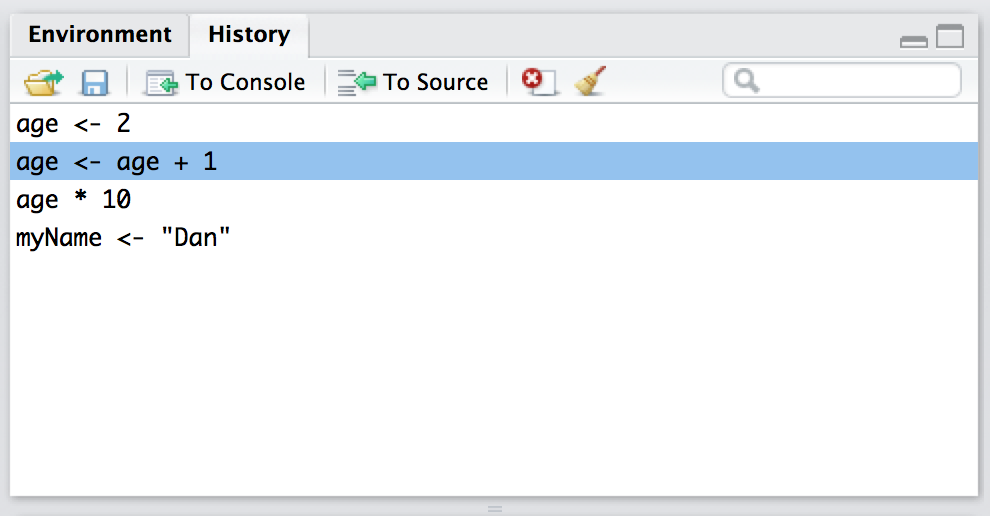
\includegraphics[width=13.75in]{/Users/dave/Documents/GitHub/stats-remix-advanced/bookdown/img/introR/historyTab} \caption{The history panel is located in the top right hand side of the RStudio window. Click on the word "History" and it displays this panel.}\label{fig:RStudiohistory}
\end{figure}

\hypertarget{vectors}{%
\section{Storing many numbers as a vector}\label{vectors}}

At this point we've covered functions in enough detail to get us safely through the next couple of chapters (with one small exception: see Section \ref{generics}, so let's return to our discussion of variables. When I introduced variables in Section \ref{assign} I showed you how we can use variables to store a single number. In this section, we'll extend this idea and look at how to store multiple numbers within the one variable. In R, the name for a variable that can store multiple values is a \textbf{\emph{vector}}. So let's create one.

\hypertarget{creating-a-vector}{%
\subsection{Creating a vector}\label{creating-a-vector}}

Let's stick to my silly ``get rich quick by textbook writing'' example. Suppose the textbook company (if I actually had one, that is) sends me sales data on a monthly basis. Since my class start in late February, we might expect most of the sales to occur towards the start of the year. Let's suppose that I have 100 sales in February, 200 sales in March and 50 sales in April, and no other sales for the rest of the year. What I would like to do is have a variable -- let's call it \texttt{sales.by.month} -- that stores all this sales data. The first number stored should be \texttt{0} since I had no sales in January, the second should be \texttt{100}, and so on. The simplest way to do this in R is to use the \textbf{\emph{combine}} function, \texttt{c()}. To do so, all we have to do is type all the numbers you want to store in a comma separated list, like this:\footnote{Notice that I didn't specify any argument names here. The \texttt{c()} function is one of those cases where we don't use names. We just type all the numbers, and R just dumps them all in a single variable.}

\begin{Shaded}
\begin{Highlighting}[]
\NormalTok{sales.by.month }\OtherTok{\textless{}{-}} \FunctionTok{c}\NormalTok{(}\DecValTok{0}\NormalTok{, }\DecValTok{100}\NormalTok{, }\DecValTok{200}\NormalTok{, }\DecValTok{50}\NormalTok{, }\DecValTok{0}\NormalTok{, }\DecValTok{0}\NormalTok{, }\DecValTok{0}\NormalTok{, }\DecValTok{0}\NormalTok{, }\DecValTok{0}\NormalTok{, }\DecValTok{0}\NormalTok{, }\DecValTok{0}\NormalTok{, }\DecValTok{0}\NormalTok{)}
\NormalTok{sales.by.month}
\end{Highlighting}
\end{Shaded}

\begin{verbatim}
##  [1]   0 100 200  50   0   0   0   0   0   0   0   0
\end{verbatim}

To use the correct terminology here, we have a single variable here called \texttt{sales.by.month}: this variable is a vector that consists of 12 \textbf{\emph{elements}}.

\hypertarget{a-handy-digression}{%
\subsection{A handy digression}\label{a-handy-digression}}

Now that we've learned how to put information into a vector, the next thing to understand is how to pull that information back out again. However, before I do so it's worth taking a slight detour. If you've been following along, typing all the commands into R yourself, it's possible that the output that you saw when we printed out the \texttt{sales.by.month} vector was slightly different to what I showed above. This would have happened if the window (or the RStudio panel) that contains the R console is really, really narrow. If that were the case, you might have seen output that looks something like this:

\begin{Shaded}
\begin{Highlighting}[]
\NormalTok{sales.by.month}
\end{Highlighting}
\end{Shaded}

\begin{verbatim}
##  [1]   0 100 200  50
##  [5]   0   0   0   0
##  [9]   0   0   0   0
\end{verbatim}

Because there wasn't much room on the screen, R has printed out the results over three lines. But that's not the important thing to notice. The important point is that the first line has a \texttt{{[}1{]}} in front of it, whereas the second line starts with \texttt{{[}5{]}} and the third with \texttt{{[}9{]}}. It's pretty clear what's happening here. For the first row, R has printed out the 1st element through to the 4th element, so it starts that row with a \texttt{{[}1{]}}. For the second row, R has printed out the 5th element of the vector through to the 8th one, and so it begins that row with a \texttt{{[}5{]}} so that you can tell where it's up to at a glance. It might seem a bit odd to you that R does this, but in some ways it's a kindness, especially when dealing with larger data sets!

\hypertarget{vectorsubset}{%
\subsection{Getting information out of vectors}\label{vectorsubset}}

To get back to the main story, let's consider the problem of how to get information out of a vector. At this point, you might have a sneaking suspicion that the answer has something to do with the \texttt{{[}1{]}} and \texttt{{[}9{]}} things that R has been printing out. And of course you are correct. Suppose I want to pull out the February sales data only. February is the second month of the year, so let's try this:

\begin{Shaded}
\begin{Highlighting}[]
\NormalTok{sales.by.month[}\DecValTok{2}\NormalTok{]}
\end{Highlighting}
\end{Shaded}

\begin{verbatim}
## [1] 100
\end{verbatim}

Yep, that's the February sales all right. But there's a subtle detail to be aware of here: notice that R outputs \texttt{{[}1{]}\ 100}, \emph{not} \texttt{{[}2{]}\ 100}. This is because R is being extremely literal. When we typed in \texttt{sales.by.month{[}2{]}}, we asked R to find exactly \emph{one} thing, and that one thing happens to be the second element of our \texttt{sales.by.month} vector. So, when it outputs \texttt{{[}1{]}\ 100} what R is saying is that the first number \emph{that we just asked for} is \texttt{100}. This behaviour makes more sense when you realise that we can use this trick to create new variables. For example, I could create a \texttt{february.sales} variable like this:

\begin{Shaded}
\begin{Highlighting}[]
\NormalTok{february.sales }\OtherTok{\textless{}{-}}\NormalTok{ sales.by.month[}\DecValTok{2}\NormalTok{]}
\NormalTok{february.sales}
\end{Highlighting}
\end{Shaded}

\begin{verbatim}
## [1] 100
\end{verbatim}

Obviously, the new variable \texttt{february.sales} should only have one element and so when I print it out this new variable, the R output begins with a \texttt{{[}1{]}} because \texttt{100} is the value of the first (and only) element of \texttt{february.sales}. The fact that this also happens to be the value of the second element of \texttt{sales.by.month} is irrelevant. We'll pick this topic up again shortly (Section \ref{indexing}).

\hypertarget{altering-the-elements-of-a-vector}{%
\subsection{Altering the elements of a vector}\label{altering-the-elements-of-a-vector}}

Sometimes you'll want to change the values stored in a vector. Imagine my surprise when the publisher rings me up to tell me that the sales data for May are wrong. There were actually an additional 25 books sold in May, but there was an error or something so they hadn't told me about it. How can I fix my \texttt{sales.by.month} variable? One possibility would be to assign the whole vector again from the beginning, using \texttt{c()}. But that's a lot of typing. Also, it's a little wasteful: why should R have to redefine the sales figures for all 12 months, when only the 5th one is wrong? Fortunately, we can tell R to change only the 5th element, using this trick:

\begin{Shaded}
\begin{Highlighting}[]
\NormalTok{sales.by.month[}\DecValTok{5}\NormalTok{] }\OtherTok{\textless{}{-}} \DecValTok{25}
\NormalTok{sales.by.month}
\end{Highlighting}
\end{Shaded}

\begin{verbatim}
##  [1]   0 100 200  50  25   0   0   0   0   0   0   0
\end{verbatim}

Another way to edit variables is to use the \texttt{edit()} or \texttt{fix()} functions. I won't discuss them in detail right now, but you can check them out on your own.

\hypertarget{veclength}{%
\subsection{Useful things to know about vectors}\label{veclength}}

Before moving on, I want to mention a couple of other things about vectors. Firstly, you often find yourself wanting to know how many elements there are in a vector (usually because you've forgotten). You can use the \texttt{length()} function to do this. It's quite straightforward:

\begin{Shaded}
\begin{Highlighting}[]
\FunctionTok{length}\NormalTok{( }\AttributeTok{x =}\NormalTok{ sales.by.month )}
\end{Highlighting}
\end{Shaded}

\begin{verbatim}
## [1] 12
\end{verbatim}

Secondly, you often want to alter all of the elements of a vector at once. For instance, suppose I wanted to figure out how much money I made in each month. Since I'm earning an exciting \$7 per book (no seriously, that's actually pretty close to what authors get on the very expensive textbooks that you're expected to purchase), what I want to do is multiply each element in the \texttt{sales.by.month} vector by \texttt{7}. R makes this pretty easy, as the following example shows:

\begin{Shaded}
\begin{Highlighting}[]
\NormalTok{sales.by.month }\SpecialCharTok{*} \DecValTok{7}
\end{Highlighting}
\end{Shaded}

\begin{verbatim}
##  [1]    0  700 1400  350  175    0    0    0    0    0    0    0
\end{verbatim}

In other words, when you multiply a vector by a single number, all elements in the vector get multiplied. The same is true for addition, subtraction, division and taking powers. So that's neat. On the other hand, suppose I wanted to know how much money I was making per day, rather than per month. Since not every month has the same number of days, I need to do something slightly different. Firstly, I'll create two new vectors:

\begin{Shaded}
\begin{Highlighting}[]
\NormalTok{days.per.month }\OtherTok{\textless{}{-}} \FunctionTok{c}\NormalTok{(}\DecValTok{31}\NormalTok{, }\DecValTok{28}\NormalTok{, }\DecValTok{31}\NormalTok{, }\DecValTok{30}\NormalTok{, }\DecValTok{31}\NormalTok{, }\DecValTok{30}\NormalTok{, }\DecValTok{31}\NormalTok{, }\DecValTok{31}\NormalTok{, }\DecValTok{30}\NormalTok{, }\DecValTok{31}\NormalTok{, }\DecValTok{30}\NormalTok{, }\DecValTok{31}\NormalTok{)}
\NormalTok{profit }\OtherTok{\textless{}{-}}\NormalTok{ sales.by.month }\SpecialCharTok{*} \DecValTok{7}
\end{Highlighting}
\end{Shaded}

Obviously, the \texttt{profit} variable is the same one we created earlier, and the \texttt{days.per.month} variable is pretty straightforward. What I want to do is divide every element of \texttt{profit} by the \emph{corresponding} element of \texttt{days.per.month}. Again, R makes this pretty easy:

\begin{Shaded}
\begin{Highlighting}[]
\NormalTok{profit }\SpecialCharTok{/}\NormalTok{ days.per.month}
\end{Highlighting}
\end{Shaded}

\begin{verbatim}
##  [1]  0.000000 25.000000 45.161290 11.666667  5.645161  0.000000  0.000000
##  [8]  0.000000  0.000000  0.000000  0.000000  0.000000
\end{verbatim}

I still don't like all those zeros, but that's not what matters here. Notice that the second element of the output is 25, because R has divided the second element of \texttt{profit} (i.e.~700) by the second element of \texttt{days.per.month} (i.e.~28). Similarly, the third element of the output is equal to 1400 divided by 31, and so on. We'll talk more about calculations involving vectors later on (and in particular a thing called the ``recycling rule''; Section \ref{recycling}), but that's enough detail for now.

\hypertarget{text}{%
\section{Storing text data}\label{text}}

A lot of the time your data will be numeric in nature, but not always. Sometimes your data really needs to be described using text, not using numbers. To address this, we need to consider the situation where our variables store text. To create a variable that stores the word ``hello'', we can type this:

\begin{Shaded}
\begin{Highlighting}[]
\NormalTok{greeting }\OtherTok{\textless{}{-}} \StringTok{"hello"}
\NormalTok{greeting}
\end{Highlighting}
\end{Shaded}

\begin{verbatim}
## [1] "hello"
\end{verbatim}

When interpreting this, it's important to recognise that the quote marks here \emph{aren't} part of the string itself. They're just something that we use to make sure that R knows to treat the characters that they enclose as a piece of text data, known as a \textbf{\emph{character string}}. In other words, R treats \texttt{"hello"} as a string containing the word ``hello''; but if I had typed \texttt{hello} instead, R would go looking for a variable by that name! You can also use \texttt{\textquotesingle{}hello\textquotesingle{}} to specify a character string.

Okay, so that's how we store the text. Next, it's important to recognise that when we do this, R stores the entire word \texttt{"hello"} as a \emph{single} element: our \texttt{greeting} variable is \emph{not} a vector of five different letters. Rather, it has only the one element, and that element corresponds to the entire character string \texttt{"hello"}. To illustrate this, if I actually ask R to find the first element of \texttt{greeting}, it prints the whole string:

\begin{Shaded}
\begin{Highlighting}[]
\NormalTok{greeting[}\DecValTok{1}\NormalTok{]}
\end{Highlighting}
\end{Shaded}

\begin{verbatim}
## [1] "hello"
\end{verbatim}

Of course, there's no reason why I can't create a vector of character strings. For instance, if we were to continue with the example of my attempts to look at the monthly sales data for my book, one variable I might want would include the names of all 12 \texttt{months}.\footnote{Though actually there's no real need to do this, since R has an inbuilt variable called \texttt{month.name} that you can use for this purpose.} To do so, I could type in a command like this

\begin{Shaded}
\begin{Highlighting}[]
\NormalTok{months }\OtherTok{\textless{}{-}} \FunctionTok{c}\NormalTok{(}\StringTok{"January"}\NormalTok{, }\StringTok{"February"}\NormalTok{, }\StringTok{"March"}\NormalTok{, }\StringTok{"April"}\NormalTok{, }\StringTok{"May"}\NormalTok{, }\StringTok{"June"}\NormalTok{,}
            \StringTok{"July"}\NormalTok{, }\StringTok{"August"}\NormalTok{, }\StringTok{"September"}\NormalTok{, }\StringTok{"October"}\NormalTok{, }\StringTok{"November"}\NormalTok{, }
            \StringTok{"December"}\NormalTok{)}
\end{Highlighting}
\end{Shaded}

This is a \textbf{\emph{character vector}} containing 12 elements, each of which is the name of a month. So if I wanted R to tell me the name of the fourth month, all I would do is this:

\begin{Shaded}
\begin{Highlighting}[]
\NormalTok{months[}\DecValTok{4}\NormalTok{]}
\end{Highlighting}
\end{Shaded}

\begin{verbatim}
## [1] "April"
\end{verbatim}

\hypertarget{simpletext}{%
\subsection{Working with text}\label{simpletext}}

Working with text data is somewhat more complicated than working with numeric data, and I discuss some of the basic ideas in Section \ref{textprocessing}, but for purposes of the current chapter we only need this bare bones sketch. The only other thing I want to do before moving on is show you an example of a function that can be applied to text data. So far, most of the functions that we have seen (i.e., \texttt{sqrt()}, \texttt{abs()} and \texttt{round()}) only make sense when applied to numeric data (e.g., you can't calculate the square root of ``hello''), and we've seen one function that can be applied to pretty much any variable or vector (i.e., \texttt{length()}). So it might be nice to see an example of a function that can be applied to text.

The function I'm going to introduce you to is called \texttt{nchar()}, and what it does is count the number of individual characters that make up a string. Recall earlier that when we tried to calculate the \texttt{length()} of our \texttt{greeting} variable it returned a value of \texttt{1}: the \texttt{greeting} variable contains only the one string, which happens to be \texttt{"hello"}. But what if I want to know how many letters there are in the word? Sure, I could \emph{count} them, but that's boring, and more to the point it's a terrible strategy if what I wanted to know was the number of letters in \emph{War and Peace}. That's where the \texttt{nchar()} function is helpful:

\begin{Shaded}
\begin{Highlighting}[]
\FunctionTok{nchar}\NormalTok{( }\AttributeTok{x =}\NormalTok{ greeting )}
\end{Highlighting}
\end{Shaded}

\begin{verbatim}
## [1] 5
\end{verbatim}

That makes sense, since there are in fact 5 letters in the string \texttt{"hello"}. Better yet, you can apply \texttt{nchar()} to whole vectors. So, for instance, if I want R to tell me how many letters there are in the names of each of the 12 months, I can do this:

\begin{Shaded}
\begin{Highlighting}[]
\FunctionTok{nchar}\NormalTok{( }\AttributeTok{x =}\NormalTok{ months )}
\end{Highlighting}
\end{Shaded}

\begin{verbatim}
##  [1] 7 8 5 5 3 4 4 6 9 7 8 8
\end{verbatim}

So that's nice to know. The \texttt{nchar()} function can do a bit more than this, and there's a lot of other functions that you can do to extract more information from text or do all sorts of fancy things. However, the goal here is not to teach any of that! The goal right now is just to see an example of a function that actually does work when applied to text.

\hypertarget{logicals}{%
\section{Storing ``true or false'' data}\label{logicals}}

Time to move onto a third kind of data. A key concept in that a lot of R relies on is the idea of a \textbf{\emph{logical value}}. A logical value is an assertion about whether something is true or false. This is implemented in R in a pretty straightforward way. There are two logical values, namely \texttt{TRUE} and \texttt{FALSE}. Despite the simplicity, a logical values are very useful things. Let's see how they work.

\hypertarget{assessing-mathematical-truths}{%
\subsection{Assessing mathematical truths}\label{assessing-mathematical-truths}}

In George Orwell's classic book \emph{1984}, one of the slogans used by the totalitarian Party was ``two plus two equals five'', the idea being that the political domination of human freedom becomes complete when it is possible to subvert even the most basic of truths. It's a terrifying thought, especially when the protagonist Winston Smith finally breaks down under torture and agrees to the proposition. ``Man is infinitely malleable'', the book says. I'm pretty sure that this isn't true of humans\footnote{I offer up my teenage attempts to be ``cool'' as evidence that some things just can't be done.} but it's definitely not true of R. R is not infinitely malleable. It has rather firm opinions on the topic of what is and isn't true, at least as regards basic mathematics. If I ask it to calculate \texttt{2\ +\ 2}, it always gives the same answer, and it's not bloody 5:

\begin{Shaded}
\begin{Highlighting}[]
\DecValTok{2} \SpecialCharTok{+} \DecValTok{2}
\end{Highlighting}
\end{Shaded}

\begin{verbatim}
## [1] 4
\end{verbatim}

Of course, so far R is just doing the calculations. I haven't asked it to explicitly assert that \(2+2 = 4\) is a true statement. If I want R to make an explicit judgement, I can use a command like this:

\begin{Shaded}
\begin{Highlighting}[]
\DecValTok{2} \SpecialCharTok{+} \DecValTok{2} \SpecialCharTok{==} \DecValTok{4}
\end{Highlighting}
\end{Shaded}

\begin{verbatim}
## [1] TRUE
\end{verbatim}

What I've done here is use the \textbf{\emph{equality operator}}, \texttt{==}, to force R to make a ``true or false'' judgement.\footnote{Note that this is a very different operator to the assignment operator \texttt{=} that I talked about in Section \ref{assign}. A common typo that people make when trying to write logical commands in R (or other languages, since the ``\texttt{=} versus \texttt{==}'' distinction is important in most programming languages) is to accidentally type \texttt{=} when you really mean \texttt{==}. Be especially cautious with this -- I've been programming in various languages since I was a teenager, and I \emph{still} screw this up a lot. Hm. I think I see why I wasn't cool as a teenager. And why I'm still not cool.} Okay, let's see what R thinks of the Party slogan:

\begin{Shaded}
\begin{Highlighting}[]
\DecValTok{2}\SpecialCharTok{+}\DecValTok{2} \SpecialCharTok{==} \DecValTok{5}
\end{Highlighting}
\end{Shaded}

\begin{verbatim}
## [1] FALSE
\end{verbatim}

Booyah! Freedom and ponies for all! Or something like that. Anyway, it's worth having a look at what happens if I try to \emph{force} R to believe that two plus two is five by making an assignment statement like \texttt{2\ +\ 2\ =\ 5} or \texttt{2\ +\ 2\ \textless{}-\ 5}. When I do this, here's what happens:

\begin{Shaded}
\begin{Highlighting}[]
\DecValTok{2} \SpecialCharTok{+} \DecValTok{2} \OtherTok{=} \DecValTok{5}
\end{Highlighting}
\end{Shaded}

\begin{verbatim}
## Error in 2 + 2 = 5: target of assignment expands to non-language object
\end{verbatim}

R doesn't like this very much. It recognises that \texttt{2\ +\ 2} is \emph{not} a variable (that's what the ``non-language object'' part is saying), and it won't let you try to ``reassign'' it. While R is pretty flexible, and actually does let you do some quite remarkable things to redefine parts of R itself, there are just some basic, primitive truths that it refuses to give up. It won't change the laws of addition, and it won't change the definition of the number \texttt{2}.

That's probably for the best.

\hypertarget{logical-operations}{%
\subsection{Logical operations}\label{logical-operations}}

So now we've seen logical operations at work, but so far we've only seen the simplest possible example. You probably won't be surprised to discover that we can combine logical operations with other operations and functions in a more complicated way, like this:

\begin{Shaded}
\begin{Highlighting}[]
\DecValTok{3}\SpecialCharTok{*}\DecValTok{3} \SpecialCharTok{+} \DecValTok{4}\SpecialCharTok{*}\DecValTok{4} \SpecialCharTok{==} \DecValTok{5}\SpecialCharTok{*}\DecValTok{5}
\end{Highlighting}
\end{Shaded}

\begin{verbatim}
## [1] TRUE
\end{verbatim}

or this

\begin{Shaded}
\begin{Highlighting}[]
\FunctionTok{sqrt}\NormalTok{( }\DecValTok{25}\NormalTok{ ) }\SpecialCharTok{==} \DecValTok{5}
\end{Highlighting}
\end{Shaded}

\begin{verbatim}
## [1] TRUE
\end{verbatim}

Not only that, but as Table \ref{tab:logicals} illustrates, there are several other logical operators that you can use, corresponding to some basic mathematical concepts.

\begin{table}

\caption{\label{tab:logicals}Some logical operators. Technically I should be calling these "binary relational operators", but quite frankly I don't want to. It's my book so no-one can make me.}
\centering
\begin{tabular}[t]{llll}
\toprule
operation & operator & example input & answer\\
\midrule
less than & < & 2 < 3 & `TRUE`\\
less than or equal to & <= & 2 <= 2 & `TRUE`\\
greater than & > & 2 > 3 & `FALSE`\\
greater than or equal to & >= & 2 >= 2 & `TRUE`\\
equal to & == & 2 == 3 & `FALSE`\\
\addlinespace
not equal to & != & 2 != 3 & `TRUE`\\
\bottomrule
\end{tabular}
\end{table}

Hopefully these are all pretty self-explanatory: for example, the \textbf{\emph{less than}} operator \texttt{\textless{}} checks to see if the number on the left is less than the number on the right. If it's less, then R returns an answer of \texttt{TRUE}:

\begin{Shaded}
\begin{Highlighting}[]
\DecValTok{99} \SpecialCharTok{\textless{}} \DecValTok{100}
\end{Highlighting}
\end{Shaded}

\begin{verbatim}
## [1] TRUE
\end{verbatim}

but if the two numbers are equal, or if the one on the right is larger, then R returns an answer of \texttt{FALSE}, as the following two examples illustrate:

\begin{Shaded}
\begin{Highlighting}[]
\DecValTok{100} \SpecialCharTok{\textless{}} \DecValTok{100}
\end{Highlighting}
\end{Shaded}

\begin{verbatim}
## [1] FALSE
\end{verbatim}

\begin{Shaded}
\begin{Highlighting}[]
\DecValTok{100} \SpecialCharTok{\textless{}} \DecValTok{99}
\end{Highlighting}
\end{Shaded}

\begin{verbatim}
## [1] FALSE
\end{verbatim}

In contrast, the \textbf{\emph{less than or equal to}} operator \texttt{\textless{}=} will do exactly what it says. It returns a value of \texttt{TRUE} if the number of the left hand side is less than or equal to the number on the right hand side. So if we repeat the previous two examples using \texttt{\textless{}=}, here's what we get:

\begin{Shaded}
\begin{Highlighting}[]
\DecValTok{100} \SpecialCharTok{\textless{}=} \DecValTok{100}
\end{Highlighting}
\end{Shaded}

\begin{verbatim}
## [1] TRUE
\end{verbatim}

\begin{Shaded}
\begin{Highlighting}[]
\DecValTok{100} \SpecialCharTok{\textless{}=} \DecValTok{99}
\end{Highlighting}
\end{Shaded}

\begin{verbatim}
## [1] FALSE
\end{verbatim}

And at this point I hope it's pretty obvious what the \textbf{\emph{greater than}} operator \texttt{\textgreater{}} and the \textbf{\emph{greater than or equal to}} operator \texttt{\textgreater{}=} do! Next on the list of logical operators is the \textbf{\emph{not equal to}} operator \texttt{!=} which -- as with all the others -- does what it says it does. It returns a value of \texttt{TRUE} when things on either side are not identical to each other. Therefore, since \(2+2\) isn't equal to \(5\), we get:

\begin{Shaded}
\begin{Highlighting}[]
\DecValTok{2} \SpecialCharTok{+} \DecValTok{2} \SpecialCharTok{!=} \DecValTok{5}
\end{Highlighting}
\end{Shaded}

\begin{verbatim}
## [1] TRUE
\end{verbatim}

We're not quite done yet. There are three more logical operations that are worth knowing about, listed in Table \ref{tab:logicals2}.

\begin{table}

\caption{\label{tab:logicals2}Some more logical operators.}
\centering
\begin{tabular}[t]{llll}
\toprule
operation & operator & example input & answer\\
\midrule
not & ! & !(1==1) & `FALSE`\\
or & | & (1==1) | (2==3) & `TRUE`\\
and & \& & (1==1) \& (2==3) & `FALSE`\\
\bottomrule
\end{tabular}
\end{table}

These are the \textbf{\emph{not}} operator \texttt{!}, the \textbf{\emph{and}} operator \texttt{\&}, and the \textbf{\emph{or}} operator \texttt{\textbar{}}. Like the other logical operators, their behaviour is more or less exactly what you'd expect given their names. For instance, if I ask you to assess the claim that ``either \(2+2 = 4\) \emph{or} \(2+2 = 5\)'' you'd say that it's true. Since it's an ``either-or'' statement, all we need is for one of the two parts to be true. That's what the \texttt{\textbar{}} operator does:

\begin{Shaded}
\begin{Highlighting}[]
\NormalTok{(}\DecValTok{2}\SpecialCharTok{+}\DecValTok{2} \SpecialCharTok{==} \DecValTok{4}\NormalTok{) }\SpecialCharTok{|}\NormalTok{ (}\DecValTok{2}\SpecialCharTok{+}\DecValTok{2} \SpecialCharTok{==} \DecValTok{5}\NormalTok{)}
\end{Highlighting}
\end{Shaded}

\begin{verbatim}
## [1] TRUE
\end{verbatim}

On the other hand, if I ask you to assess the claim that ``both \(2+2 = 4\) \emph{and} \(2+2 = 5\)'' you'd say that it's false. Since this is an \emph{and} statement we need both parts to be true. And that's what the \texttt{\&} operator does:

\begin{Shaded}
\begin{Highlighting}[]
\NormalTok{(}\DecValTok{2}\SpecialCharTok{+}\DecValTok{2} \SpecialCharTok{==} \DecValTok{4}\NormalTok{) }\SpecialCharTok{\&}\NormalTok{ (}\DecValTok{2}\SpecialCharTok{+}\DecValTok{2} \SpecialCharTok{==} \DecValTok{5}\NormalTok{)}
\end{Highlighting}
\end{Shaded}

\begin{verbatim}
## [1] FALSE
\end{verbatim}

Finally, there's the \emph{not} operator, which is simple but annoying to describe in English. If I ask you to assess my claim that ``it is not true that \(2+2 = 5\)'' then you would say that my claim is true; because my claim is that ``\(2+2 = 5\) is false''. And I'm right. If we write this as an R command we get this:

\begin{Shaded}
\begin{Highlighting}[]
\SpecialCharTok{!}\NormalTok{ (}\DecValTok{2}\SpecialCharTok{+}\DecValTok{2} \SpecialCharTok{==} \DecValTok{5}\NormalTok{)}
\end{Highlighting}
\end{Shaded}

\begin{verbatim}
## [1] TRUE
\end{verbatim}

In other words, since \texttt{2+2\ ==\ 5} is a \texttt{FALSE} statement, it must be the case that \texttt{!(2+2\ ==\ 5)} is a \texttt{TRUE} one. Essentially, what we've really done is claim that ``not false'' is the same thing as ``true''. Obviously, this isn't really quite right in real life. But R lives in a much more black or white world: for R everything is either true or false. No shades of gray are allowed. We can actually see this much more explicitly, like this:

\begin{Shaded}
\begin{Highlighting}[]
\SpecialCharTok{!} \ConstantTok{FALSE}
\end{Highlighting}
\end{Shaded}

\begin{verbatim}
## [1] TRUE
\end{verbatim}

Of course, in our \(2+2 = 5\) example, we didn't really need to use ``not'' \texttt{!} and ``equals to'' \texttt{==} as two separate operators. We could have just used the ``not equals to'' operator \texttt{!=} like this:

\begin{Shaded}
\begin{Highlighting}[]
\DecValTok{2}\SpecialCharTok{+}\DecValTok{2} \SpecialCharTok{!=} \DecValTok{5}
\end{Highlighting}
\end{Shaded}

\begin{verbatim}
## [1] TRUE
\end{verbatim}

But there are many situations where you really do need to use the \texttt{!} operator. We'll see some later on.\footnote{A note for those of you who have taken a computer science class: yes, R does have a function for exclusive-or, namely \texttt{xor()}. Also worth noting is the fact that R makes the distinction between element-wise operators \texttt{\&} and \texttt{\textbar{}} and operators that look only at the first element of the vector, namely \texttt{\&\&} and \texttt{\textbar{}\textbar{}}. To see the distinction, compare the behaviour of a command like \texttt{c(FALSE,TRUE)\ \&\ c(TRUE,TRUE)} to the behaviour of something like \texttt{c(FALSE,TRUE)\ \&\&\ c(TRUE,TRUE)}. If this doesn't mean anything to you, ignore this footnote entirely. It's not important for the content of this book.}

\hypertarget{storing-and-using-logical-data}{%
\subsection{Storing and using logical data}\label{storing-and-using-logical-data}}

Up to this point, I've introduced \emph{numeric data} (in Sections \ref{assign} and \ref{vectors}) and \emph{character data} (in Section \ref{text}). So you might not be surprised to discover that these \texttt{TRUE} and \texttt{FALSE} values that R has been producing are actually a third kind of data, called \emph{logical data}. That is, when I asked R if \texttt{2\ +\ 2\ ==\ 5} and it said \texttt{{[}1{]}\ FALSE} in reply, it was actually producing information that we can store in variables. For instance, I could create a variable called \texttt{is.the.Party.correct}, which would store R's opinion:

\begin{Shaded}
\begin{Highlighting}[]
\NormalTok{is.the.Party.correct }\OtherTok{\textless{}{-}} \DecValTok{2} \SpecialCharTok{+} \DecValTok{2} \SpecialCharTok{==} \DecValTok{5}
\NormalTok{is.the.Party.correct}
\end{Highlighting}
\end{Shaded}

\begin{verbatim}
## [1] FALSE
\end{verbatim}

Alternatively, you can assign the value directly, by typing \texttt{TRUE} or \texttt{FALSE} in your command. Like this:

\begin{Shaded}
\begin{Highlighting}[]
\NormalTok{is.the.Party.correct }\OtherTok{\textless{}{-}} \ConstantTok{FALSE}
\NormalTok{is.the.Party.correct}
\end{Highlighting}
\end{Shaded}

\begin{verbatim}
## [1] FALSE
\end{verbatim}

Better yet, because it's kind of tedious to type \texttt{TRUE} or \texttt{FALSE} over and over again, R provides you with a shortcut: you can use \texttt{T} and \texttt{F} instead (but it's case sensitive: \texttt{t} and \texttt{f} won't work).\footnote{Warning! \texttt{TRUE} and \texttt{FALSE} are reserved keywords in R, so you can trust that they always mean what they say they do. Unfortunately, the shortcut versions \texttt{T} and \texttt{F} do not have this property. It's even possible to create variables that set up the reverse meanings, by typing commands like \texttt{T\ \textless{}-\ FALSE} and \texttt{F\ \textless{}-\ TRUE}. This is kind of insane, and something that is generally thought to be a design flaw in R. Anyway, the long and short of it is that it's safer to use \texttt{TRUE} and \texttt{FALSE}.} So this works:

\begin{Shaded}
\begin{Highlighting}[]
\NormalTok{is.the.Party.correct }\OtherTok{\textless{}{-}}\NormalTok{ F}
\NormalTok{is.the.Party.correct}
\end{Highlighting}
\end{Shaded}

\begin{verbatim}
## [1] FALSE
\end{verbatim}

but this doesn't:

\begin{Shaded}
\begin{Highlighting}[]
\NormalTok{is.the.Party.correct }\OtherTok{\textless{}{-}}\NormalTok{ f}
\end{Highlighting}
\end{Shaded}

\begin{verbatim}
## Error in eval(expr, envir, enclos): object 'f' not found
\end{verbatim}

\hypertarget{vectors-of-logicals}{%
\subsection{Vectors of logicals}\label{vectors-of-logicals}}

The next thing to mention is that you can store vectors of logical values in exactly the same way that you can store vectors of numbers (Section \ref{vectors}) and vectors of text data (Section \ref{text}). Again, we can define them directly via the \texttt{c()} function, like this:

\begin{Shaded}
\begin{Highlighting}[]
\NormalTok{x }\OtherTok{\textless{}{-}} \FunctionTok{c}\NormalTok{(}\ConstantTok{TRUE}\NormalTok{, }\ConstantTok{TRUE}\NormalTok{, }\ConstantTok{FALSE}\NormalTok{)}
\NormalTok{x}
\end{Highlighting}
\end{Shaded}

\begin{verbatim}
## [1]  TRUE  TRUE FALSE
\end{verbatim}

or you can produce a vector of logicals by applying a logical operator to a vector. This might not make a lot of sense to you, so let's unpack it slowly. First, let's suppose we have a vector of numbers (i.e., a ``non-logical vector''). For instance, we could use the \texttt{sales.by.month} vector that we were using in Section \ref{vectors}. Suppose I wanted R to tell me, for each month of the year, whether I actually sold a book in that month. I can do that by typing this:

\begin{Shaded}
\begin{Highlighting}[]
\NormalTok{sales.by.month }\SpecialCharTok{\textgreater{}} \DecValTok{0}
\end{Highlighting}
\end{Shaded}

\begin{verbatim}
##  [1] FALSE  TRUE  TRUE  TRUE  TRUE FALSE FALSE FALSE FALSE FALSE FALSE
## [12] FALSE
\end{verbatim}

and again, I can store this in a vector if I want, as the example below illustrates:

\begin{Shaded}
\begin{Highlighting}[]
\NormalTok{any.sales.this.month }\OtherTok{\textless{}{-}}\NormalTok{ sales.by.month }\SpecialCharTok{\textgreater{}} \DecValTok{0}
\NormalTok{any.sales.this.month}
\end{Highlighting}
\end{Shaded}

\begin{verbatim}
##  [1] FALSE  TRUE  TRUE  TRUE  TRUE FALSE FALSE FALSE FALSE FALSE FALSE
## [12] FALSE
\end{verbatim}

In other words, \texttt{any.sales.this.month} is a logical vector whose elements are \texttt{TRUE} only if the corresponding element of \texttt{sales.by.month} is greater than zero. For instance, since I sold zero books in January, the first element is \texttt{FALSE}.

\hypertarget{logictext}{%
\subsection{Applying logical operation to text}\label{logictext}}

In a moment (Section \ref{indexing}) I'll show you why these logical operations and logical vectors are so handy, but before I do so I want to very briefly point out that you can apply them to text as well as to logical data. It's just that we need to be a bit more careful in understanding how R interprets the different operations. In this section I'll talk about how the equal to operator \texttt{==} applies to text, since this is the most important one. Obviously, the not equal to operator \texttt{!=} gives the exact opposite answers to \texttt{==} so I'm implicitly talking about that one too, but I won't give specific commands showing the use of \texttt{!=}. As for the other operators, I'll defer a more detailed discussion of this topic to Section \ref{logictext2}.

Okay, let's see how it works. In one sense, it's very simple. For instance, I can ask R if the word \texttt{"cat"} is the same as the word \texttt{"dog"}, like this:

\begin{Shaded}
\begin{Highlighting}[]
\StringTok{"cat"} \SpecialCharTok{==} \StringTok{"dog"}
\end{Highlighting}
\end{Shaded}

\begin{verbatim}
## [1] FALSE
\end{verbatim}

That's pretty obvious, and it's good to know that even R can figure that out. Similarly, R does recognise that a \texttt{"cat"} is a \texttt{"cat"}:

\begin{Shaded}
\begin{Highlighting}[]
\StringTok{"cat"} \SpecialCharTok{==} \StringTok{"cat"}
\end{Highlighting}
\end{Shaded}

\begin{verbatim}
## [1] TRUE
\end{verbatim}

Again, that's exactly what we'd expect. However, what you need to keep in mind is that R is not at all tolerant when it comes to grammar and spacing. If two strings differ in any way whatsoever, R will say that they're not equal to each other, as the following examples indicate:

\begin{Shaded}
\begin{Highlighting}[]
\StringTok{" cat"} \SpecialCharTok{==} \StringTok{"cat"}
\end{Highlighting}
\end{Shaded}

\begin{verbatim}
## [1] FALSE
\end{verbatim}

\begin{Shaded}
\begin{Highlighting}[]
\StringTok{"cat"} \SpecialCharTok{==} \StringTok{"CAT"}
\end{Highlighting}
\end{Shaded}

\begin{verbatim}
## [1] FALSE
\end{verbatim}

\begin{Shaded}
\begin{Highlighting}[]
\StringTok{"cat"} \SpecialCharTok{==} \StringTok{"c a t"}
\end{Highlighting}
\end{Shaded}

\begin{verbatim}
## [1] FALSE
\end{verbatim}

\hypertarget{indexing}{%
\section{Indexing vectors}\label{indexing}}

One last thing to add before finishing up this chapter. So far, whenever I've had to get information out of a vector, all I've done is typed something like \texttt{months{[}4{]}}; and when I do this R prints out the fourth element of the \texttt{months} vector. In this section, I'll show you two additional tricks for getting information out of the vector.

\hypertarget{extracting-multiple-elements}{%
\subsection{Extracting multiple elements}\label{extracting-multiple-elements}}

One very useful thing we can do is pull out more than one element at a time. In the previous example, we only used a single number (i.e., \texttt{2}) to indicate which element we wanted. Alternatively, we can use a vector. So, suppose I wanted the data for February, March and April. What I could do is use the vector \texttt{c(2,3,4)} to indicate which elements I want R to pull out. That is, I'd type this:

\begin{Shaded}
\begin{Highlighting}[]
\NormalTok{sales.by.month[ }\FunctionTok{c}\NormalTok{(}\DecValTok{2}\NormalTok{,}\DecValTok{3}\NormalTok{,}\DecValTok{4}\NormalTok{) ]}
\end{Highlighting}
\end{Shaded}

\begin{verbatim}
## [1] 100 200  50
\end{verbatim}

Notice that the order matters here. If I asked for the data in the reverse order (i.e., April first, then March, then February) by using the vector \texttt{c(4,3,2)}, then R outputs the data in the reverse order:

\begin{Shaded}
\begin{Highlighting}[]
\NormalTok{sales.by.month[ }\FunctionTok{c}\NormalTok{(}\DecValTok{4}\NormalTok{,}\DecValTok{3}\NormalTok{,}\DecValTok{2}\NormalTok{) ]}
\end{Highlighting}
\end{Shaded}

\begin{verbatim}
## [1]  50 200 100
\end{verbatim}

A second thing to be aware of is that R provides you with handy shortcuts for very common situations. For instance, suppose that I wanted to extract everything from the 2nd month through to the 8th month. One way to do this is to do the same thing I did above, and use the vector \texttt{c(2,3,4,5,6,7,8)} to indicate the elements that I want. That works just fine

\begin{Shaded}
\begin{Highlighting}[]
\NormalTok{sales.by.month[ }\FunctionTok{c}\NormalTok{(}\DecValTok{2}\NormalTok{,}\DecValTok{3}\NormalTok{,}\DecValTok{4}\NormalTok{,}\DecValTok{5}\NormalTok{,}\DecValTok{6}\NormalTok{,}\DecValTok{7}\NormalTok{,}\DecValTok{8}\NormalTok{) ]}
\end{Highlighting}
\end{Shaded}

\begin{verbatim}
## [1] 100 200  50  25   0   0   0
\end{verbatim}

but it's kind of a lot of typing. To help make this easier, R lets you use \texttt{2:8} as shorthand for \texttt{c(2,3,4,5,6,7,8)}, which makes things a lot simpler. First, let's just check that this is true:

\begin{Shaded}
\begin{Highlighting}[]
\DecValTok{2}\SpecialCharTok{:}\DecValTok{8}
\end{Highlighting}
\end{Shaded}

\begin{verbatim}
## [1] 2 3 4 5 6 7 8
\end{verbatim}

Next, let's check that we can use the \texttt{2:8} shorthand as a way to pull out the 2nd through 8th elements of \texttt{sales.by.months}:

\begin{Shaded}
\begin{Highlighting}[]
\NormalTok{sales.by.month[}\DecValTok{2}\SpecialCharTok{:}\DecValTok{8}\NormalTok{]}
\end{Highlighting}
\end{Shaded}

\begin{verbatim}
## [1] 100 200  50  25   0   0   0
\end{verbatim}

So that's kind of neat.

\hypertarget{logical-indexing}{%
\subsection{Logical indexing}\label{logical-indexing}}

At this point, I can introduce an extremely useful tool called \textbf{\emph{logical indexing}}. In the last section, I created a logical vector \texttt{any.sales.this.month}, whose elements are \texttt{TRUE} for any month in which I sold at least one book, and \texttt{FALSE} for all the others. However, that big long list of \texttt{TRUE}s and \texttt{FALSE}s is a little bit hard to read, so what I'd like to do is to have R select the names of the \texttt{months} for which I sold any books. Earlier on, I created a vector \texttt{months} that contains the names of each of the months. This is where logical indexing is handy. What I need to do is this:

\begin{Shaded}
\begin{Highlighting}[]
\NormalTok{months[ sales.by.month }\SpecialCharTok{\textgreater{}} \DecValTok{0}\NormalTok{ ]}
\end{Highlighting}
\end{Shaded}

\begin{verbatim}
## [1] "February" "March"    "April"    "May"
\end{verbatim}

To understand what's happening here, it's helpful to notice that \texttt{sales.by.month\ \textgreater{}\ 0} is the same logical expression that we used to create the \texttt{any.sales.this.month} vector in the last section. In fact, I could have just done this:

\begin{Shaded}
\begin{Highlighting}[]
\NormalTok{months[ any.sales.this.month ]}
\end{Highlighting}
\end{Shaded}

\begin{verbatim}
## [1] "February" "March"    "April"    "May"
\end{verbatim}

and gotten exactly the same result. In order to figure out which elements of \texttt{months} to include in the output, what R does is look to see if the corresponding element in \texttt{any.sales.this.month} is \texttt{TRUE}. Thus, since element 1 of \texttt{any.sales.this.month} is \texttt{FALSE}, R does not include \texttt{"January"} as part of the output; but since element 2 of \texttt{any.sales.this.month} is \texttt{TRUE}, R does include \texttt{"February"} in the output. Note that there's no reason why I can't use the same trick to find the actual sales numbers for those months. The command to do that would just be this:

\begin{Shaded}
\begin{Highlighting}[]
\NormalTok{sales.by.month [ sales.by.month }\SpecialCharTok{\textgreater{}} \DecValTok{0}\NormalTok{ ]}
\end{Highlighting}
\end{Shaded}

\begin{verbatim}
## [1] 100 200  50  25
\end{verbatim}

In fact, we can do the same thing with text. Here's an example. Suppose that -- to continue the saga of the textbook sales -- I later find out that the bookshop only had sufficient stocks for a few months of the year. They tell me that early in the year they had \texttt{"high"} stocks, which then dropped to \texttt{"low"} levels, and in fact for one month they were \texttt{"out"} of copies of the book for a while before they were able to replenish them. Thus I might have a variable called \texttt{stock.levels} which looks like this:

\begin{Shaded}
\begin{Highlighting}[]
\NormalTok{stock.levels}\OtherTok{\textless{}{-}}\FunctionTok{c}\NormalTok{(}\StringTok{"high"}\NormalTok{, }\StringTok{"high"}\NormalTok{, }\StringTok{"low"}\NormalTok{, }\StringTok{"out"}\NormalTok{, }\StringTok{"out"}\NormalTok{, }\StringTok{"high"}\NormalTok{,}
                \StringTok{"high"}\NormalTok{, }\StringTok{"high"}\NormalTok{, }\StringTok{"high"}\NormalTok{, }\StringTok{"high"}\NormalTok{, }\StringTok{"high"}\NormalTok{, }\StringTok{"high"}\NormalTok{)}

\NormalTok{stock.levels}
\end{Highlighting}
\end{Shaded}

\begin{verbatim}
##  [1] "high" "high" "low"  "out"  "out"  "high" "high" "high" "high" "high"
## [11] "high" "high"
\end{verbatim}

Thus, if I want to know the months for which the bookshop was out of my book, I could apply the logical indexing trick, but with the character vector \texttt{stock.levels}, like this:

\begin{Shaded}
\begin{Highlighting}[]
\NormalTok{months[stock.levels }\SpecialCharTok{==} \StringTok{"out"}\NormalTok{]}
\end{Highlighting}
\end{Shaded}

\begin{verbatim}
## [1] "April" "May"
\end{verbatim}

Alternatively, if I want to know when the bookshop was either low on copies or out of copies, I could do this:

\begin{Shaded}
\begin{Highlighting}[]
\NormalTok{months[stock.levels }\SpecialCharTok{==} \StringTok{"out"} \SpecialCharTok{|}\NormalTok{ stock.levels }\SpecialCharTok{==} \StringTok{"low"}\NormalTok{]}
\end{Highlighting}
\end{Shaded}

\begin{verbatim}
## [1] "March" "April" "May"
\end{verbatim}

or this

\begin{Shaded}
\begin{Highlighting}[]
\NormalTok{months[stock.levels }\SpecialCharTok{!=} \StringTok{"high"}\NormalTok{ ]}
\end{Highlighting}
\end{Shaded}

\begin{verbatim}
## [1] "March" "April" "May"
\end{verbatim}

Either way, I get the answer I want.

At this point, I hope you can see why logical indexing is such a useful thing. It's a very basic, yet very powerful way to manipulate data. We'll talk a lot more about how to manipulate data in Chapter \ref{datahandling}, since it's a critical skill for real world research that is often overlooked in introductory research methods classes (or at least, that's been my experience). It does take a bit of practice to become completely comfortable using logical indexing, so it's a good idea to play around with these sorts of commands. Try creating a few different variables of your own, and then ask yourself questions like ``how do I get R to spit out all the elements that are {[}blah{]}''. Practice makes perfect, and it's only by practicing logical indexing that you'll perfect the art of yelling frustrated insults at your computer.\footnote{Well, I say that\ldots{} but in my personal experience it wasn't until I started learning ``regular expressions'' that my loathing of computers reached its peak.}

\hypertarget{quitting-r}{%
\section{Quitting R}\label{quitting-r}}

\begin{figure}
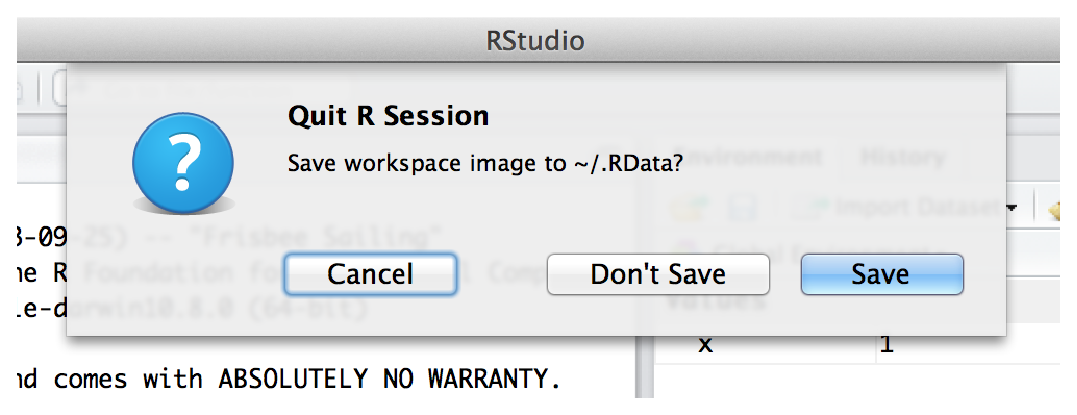
\includegraphics[width=13.92in]{/Users/dave/Documents/GitHub/stats-remix-advanced/bookdown/img/introR/Rstudio_quit} \caption{The dialog box that shows up when you try to close RStudio.}\label{fig:quitR}
\end{figure}

There's one last thing I should cover in this chapter: how to quit R. When I say this, I'm not trying to imply that R is some kind of pathological addition and that you need to call the R QuitLine or wear patches to control the cravings (although you certainly might argue that there's something seriously pathological about being addicted to R). I just mean how to exit the program. Assuming you're running R in the usual way (i.e., through RStudio or the default GUI on a Windows or Mac computer), then you can just shut down the application in the normal way. However, R also has a function, called \texttt{q()} that you can use to quit, which is pretty handy if you're running R in a terminal window.

Regardless of what method you use to quit R, when you do so for the first time R will probably ask you if you want to save the ``workspace image''. We'll talk a lot more about loading and saving data in Section \ref{load}, but I figured we'd better quickly cover this now otherwise you're going to get annoyed when you close R at the end of the chapter. If you're using RStudio, you'll see a dialog box that looks like the one shown in Figure \ref{fig:quitR}. If you're using a text based interface you'll see this:

\begin{Shaded}
\begin{Highlighting}[]
\FunctionTok{q}\NormalTok{()}

\DocumentationTok{\#\# Save workspace image? [y/n/c]: }
\end{Highlighting}
\end{Shaded}

The \texttt{y/n/c} part here is short for ``yes / no / cancel''. Type \texttt{y} if you want to save, \texttt{n} if you don't, and \texttt{c} if you've changed your mind and you don't want to quit after all.

What does this actually \emph{mean}? What's going on is that R wants to know if you want to save all those variables that you've been creating, so that you can use them later. This sounds like a great idea, so it's really tempting to type \texttt{y} or click the ``Save'' button. To be honest though, I very rarely do this, and it kind of annoys me a little bit\ldots{} what R is \emph{really} asking is if you want it to store these variables in a ``default'' data file, which it will automatically reload for you next time you open R. And quite frankly, if I'd wanted to save the variables, then I'd have already saved them before trying to quit. Not only that, I'd have saved them to a location of \emph{my} choice, so that I can find it again later. So I personally never bother with this.

In fact, every time I install R on a new machine one of the first things I do is change the settings so that it never asks me again. You can do this in RStudio really easily: use the menu system to find the RStudio option; the dialog box that comes up will give you an option to tell R never to whine about this again (see Figure \ref{fig:RStudiooptions}. On a Mac, you can open this window by going to the ``RStudio'' menu and selecting ``Preferences''. On a Windows machine you go to the ``Tools'' menu and select ``Global Options''. Under the ``General'' tab you'll see an option that reads ``Save workspace to .Rdata on exit''. By default this is set to ``ask''. If you want R to stop asking, change it to ``never''.

\begin{figure}
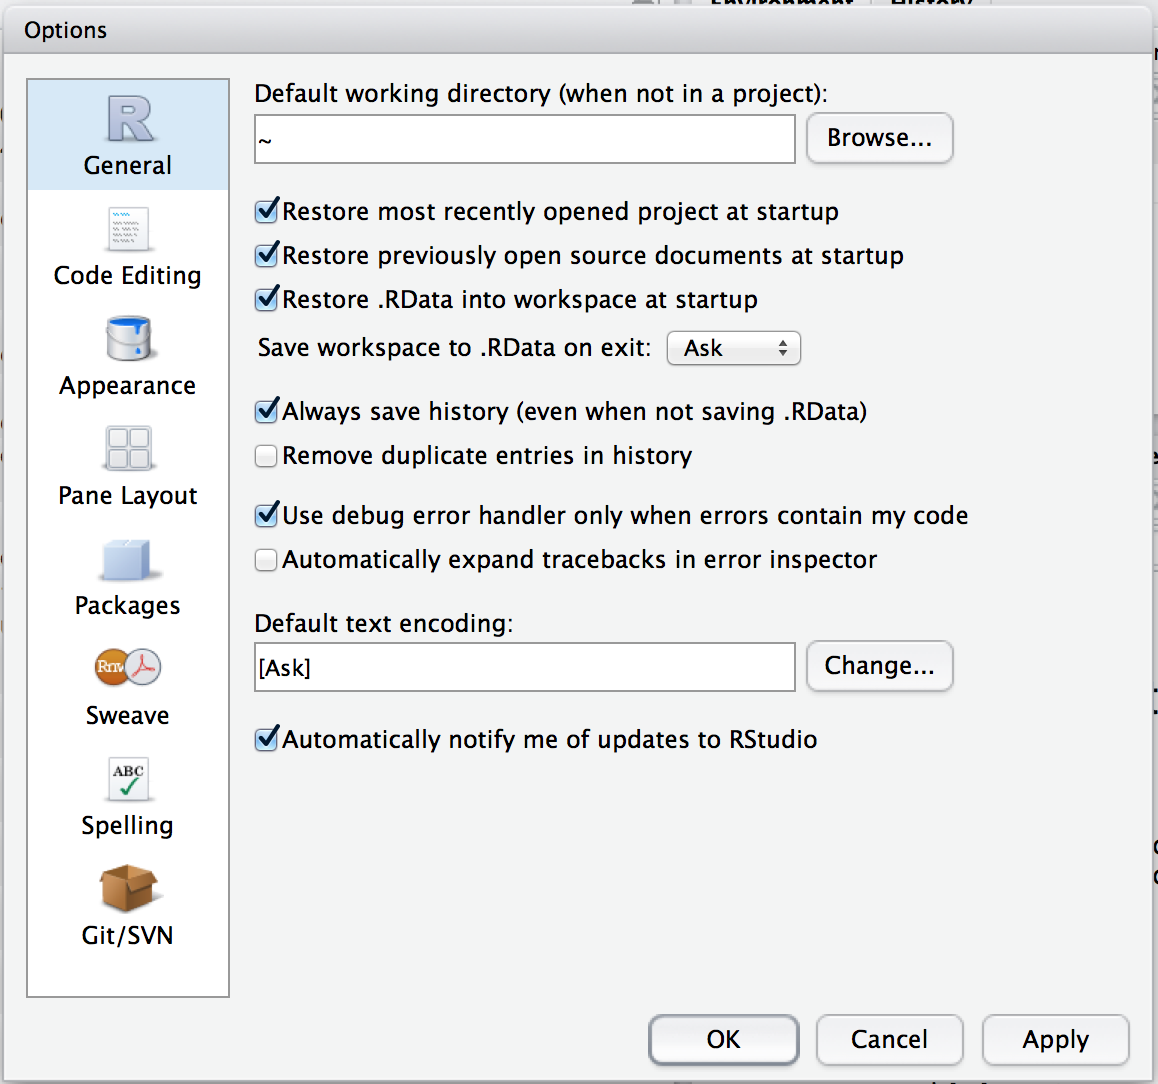
\includegraphics[width=16.08in]{/Users/dave/Documents/GitHub/stats-remix-advanced/bookdown/img/introR/Rstudio_options} \caption{The options window in RStudio. On a Mac, you can open this window by going to the "RStudio" menu and selecting "Preferences". On a Windows machine you go to the "Tools" menu and select "Global Options"}\label{fig:RStudiooptions}
\end{figure}

\hypertarget{summary}{%
\section{Summary}\label{summary}}

Every book that tries to introduce basic programming ideas to novices has to cover roughly the same topics, and in roughly the same order. Mine is no exception, and so in the grand tradition of doing it just the same way everyone else did it, this chapter covered the following topics:

\begin{itemize}
\tightlist
\item
  \protect\hyperlink{gettingR}{Getting started}. We downloaded and installed R and RStudio
\item
  \protect\hyperlink{arithmetic}{Basic commands}. We talked a bit about the logic of how R works and in particular how to type commands into the R console (Section @ref(\#firstcommand), and in doing so learned how to perform basic calculations using the arithmetic operators \texttt{+}, \texttt{-}, \texttt{*}, \texttt{/} and \texttt{\^{}}.
\item
  \protect\hyperlink{usingfunctions}{Introduction to functions}. We saw several different functions, three that are used to perform numeric calculations (\texttt{sqrt()}, \texttt{abs()}, \texttt{round()}, one that applies to text (\texttt{nchar()}; Section \ref{simpletext}), and one that works on any variable (\texttt{length()}; Section \ref{veclength}). In doing so, we talked a bit about how argument names work, and learned about default values for arguments. (Section \ref{functionarguments})
\item
  Introduction to variables. We learned the basic idea behind variables, and how to assign values to variables using the assignment operator \texttt{\textless{}-} (Section \ref{assign}). We also learned how to create vectors using the combine function \texttt{c()} (Section \ref{vectors}).
\item
  Data types. Learned the distinction between numeric, character and logical data; including the basics of how to enter and use each of them. (Sections \ref{assign} to \ref{logicals})
\item
  \protect\hyperlink{logicals}{Logical operations}. Learned how to use the logical operators \texttt{==}, \texttt{!=}, \texttt{\textless{}}, \texttt{\textgreater{}}, \texttt{\textless{}=}, \texttt{=\textgreater{}}, \texttt{!}, \texttt{\&} and \texttt{\textbar{}}. And learned how to use logical indexing. (Section \ref{indexing})
\end{itemize}

We still haven't arrived at anything that resembles a ``data set'', of course. Maybe the next Chapter will get us a bit closer\ldots{}

\hypertarget{mechanics}{%
\section{Additional R concepts}\label{mechanics}}

\begin{quote}
\emph{Form follows function}

-- Louis Sullivan
\end{quote}

So far, our main goal was to get started in R. As we go through the book we'll run into a lot of new R concepts, which I'll explain alongside the relevant data analysis concepts. However, there's still quite a few things that I need to talk about now, otherwise we'll run into problems when we start trying to work with data and do statistics. So that's the goal in this section: to build on the introductory content from the last section, to get you to the point that we can start using R for statistics. Broadly speaking, the section comes in two parts. The first half of the section is devoted to the ``mechanics'' of R: installing and loading packages, managing the workspace, navigating the file system, and loading and saving data. In the second half, I'll talk more about what kinds of variables exist in R, and introduce three new kinds of variables: factors, data frames and formulas. I'll finish up by talking a little bit about the help documentation in R as well as some other avenues for finding assistance. In general, I'm not trying to be comprehensive in this chapter, I'm trying to make sure that you've got the basic foundations needed to tackle the content that comes later in the book. However, a lot of the topics are revisited in more detail later, especially in Chapters \ref{datahandling} and \ref{scripting}.

\hypertarget{comments}{%
\section{Using comments}\label{comments}}

Before discussing any of the more complicated stuff, I want to introduce the \textbf{\emph{comment}} character, \texttt{\#}. It has a simple meaning: it tells R to ignore everything else you've written on this line. You won't have much need of the \texttt{\#} character immediately, but it's very useful later on when writing scripts (see Chapter \ref{scripting}). However, while you don't need to use it, I want to be able to include comments in my R extracts. For instance, if you read this:\footnote{Notice that I used \texttt{print(keeper)} rather than just typing \texttt{keeper}. Later on in the text I'll sometimes use the \texttt{print()} function to display things because I think it helps make clear what I'm doing, but in practice people rarely do this.}

\begin{Shaded}
\begin{Highlighting}[]
\NormalTok{seeker }\OtherTok{\textless{}{-}} \FloatTok{3.1415}           \CommentTok{\# create the first variable}
\NormalTok{lover }\OtherTok{\textless{}{-}} \FloatTok{2.7183}            \CommentTok{\# create the second variable}
\NormalTok{keeper }\OtherTok{\textless{}{-}}\NormalTok{ seeker }\SpecialCharTok{*}\NormalTok{ lover   }\CommentTok{\# now multiply them to create a third one}
\FunctionTok{print}\NormalTok{( keeper )            }\CommentTok{\# print out the value of \textquotesingle{}keeper\textquotesingle{}}
\end{Highlighting}
\end{Shaded}

\begin{verbatim}
## [1] 8.539539
\end{verbatim}

it's a lot easier to understand what I'm doing than if I just write this:

\begin{Shaded}
\begin{Highlighting}[]
\NormalTok{seeker }\OtherTok{\textless{}{-}} \FloatTok{3.1415}
\NormalTok{lover }\OtherTok{\textless{}{-}} \FloatTok{2.7183}
\NormalTok{keeper }\OtherTok{\textless{}{-}}\NormalTok{ seeker }\SpecialCharTok{*}\NormalTok{ lover}
\FunctionTok{print}\NormalTok{( keeper )    }
\end{Highlighting}
\end{Shaded}

\begin{verbatim}
## [1] 8.539539
\end{verbatim}

You might have already noticed that the code extracts in Chapter \ref{introR} included the \texttt{\#} character, but from now on, you'll start seeing \texttt{\#} characters appearing in the extracts, with some human-readable explanatory remarks next to them. These are still perfectly legitimate commands, since R knows that it should ignore the \texttt{\#} character and everything after it. But hopefully they'll help make things a little easier to understand.

\hypertarget{packageinstall}{%
\section{Installing and loading packages}\label{packageinstall}}

In this section I discuss R \textbf{\emph{packages}}, since almost all of the functions you might want to use in R come in packages. A package is basically just a big collection of functions, data sets and other R objects that are all grouped together under a common name. Some packages are already installed when you put R on your computer, but the vast majority of them of R packages are out there on the internet, waiting for you to download, install and use them.

When I first started writing this book, RStudio didn't really exist as a viable option for using R, and as a consequence I wrote a very lengthy section that explained how to do package management using raw R commands. It's not actually terribly hard to work with packages that way, but it's clunky and unpleasant. Fortunately, we don't have to do things that way anymore. In this section, I'll describe how to work with packages using the RStudio tools, because they're so much simpler. Along the way, you'll see that whenever you get RStudio to do something (e.g., install a package), you'll actually see the R commands that get created. I'll explain them as we go, because I think that helps you understand what's going on.

However, before we get started, there's a critical distinction that you need to understand, which is the difference between having a package \textbf{\emph{installed}} on your computer, and having a package \textbf{\emph{loaded}} in R. As of this writing, there are just over 5000 R packages freely available ``out there'' on the internet.\footnote{More precisely, there are 5000 or so packages on CRAN, the Comprehensive R Archive Network.} When you install R on your computer, you don't get all of them: only about 30 or so come bundled with the basic R installation. So right now there are about 30 packages ``installed'' on your computer, and another 5000 or so that are not installed. So that's what installed means: it means ``it's on your computer somewhere''. The critical thing to remember is that just because something is on your computer doesn't mean R can use it. In order for R to be able to \emph{use} one of your 30 or so installed packages, that package must also be ``loaded''. Generally, when you open up R, only a few of these packages (about 7 or 8) are actually loaded. Basically what it boils down to is this:

\begin{quote}
A package must be installed before it can be loaded.
\end{quote}

\begin{quote}
A package must be loaded before it can be used.
\end{quote}

This two step process might seem a little odd at first, but the designers of R had very good reasons to do it this way,\footnote{Basically, the reason is that there are 5000 packages, and probably about 4000 authors of packages, and no-one really knows what all of them do. Keeping the installation separate from the loading minimizes the chances that two packages will interact with each other in a nasty way.} and you get the hang of it pretty quickly.

\hypertarget{the-package-panel-in-rstudio}{%
\subsection{The package panel in RStudio}\label{the-package-panel-in-rstudio}}

\begin{figure}
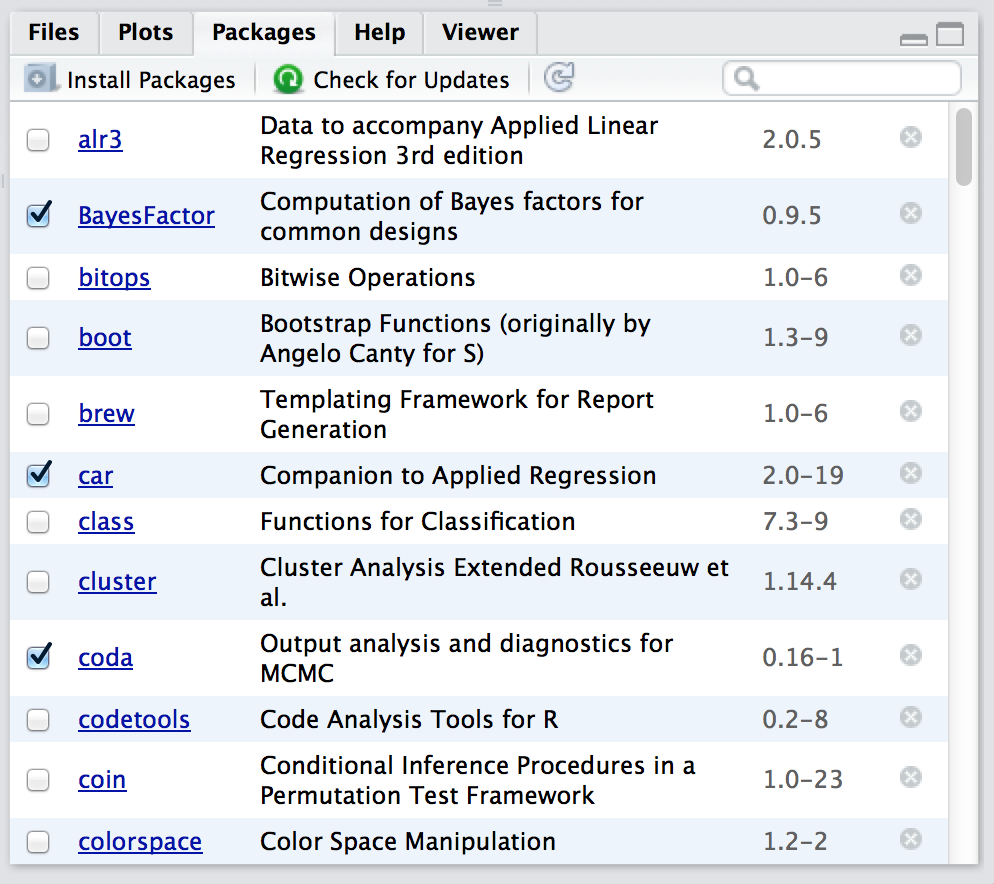
\includegraphics[width=13.81in]{/Users/dave/Documents/GitHub/stats-remix-advanced/bookdown/img/mechanics/Rstudiopackages} \caption{The packages panel.}\label{fig:packagepanel}
\end{figure}

Right, lets get started. The first thing you need to do is look in the lower right hand panel in RStudio. You'll see a tab labelled ``Packages''. Click on the tab, and you'll see a list of packages that looks something like Figure \ref{fig:packagepanel}. Every row in the panel corresponds to a different package, and every column is a useful piece of information about that package.\footnote{If you're using the command line, you can get the same information by typing \texttt{library()} at the command line.} Going from left to right, here's what each column is telling you:

\begin{itemize}
\tightlist
\item
  The check box on the far left column indicates whether or not the package is loaded.
\item
  The one word of text immediately to the right of the check box is the name of the package.
\item
  The short passage of text next to the name is a brief description of the package.
\item
  The number next to the description tells you what version of the package you have installed.
\item
  The little x-mark next to the version number is a button that you can push to uninstall the package from your computer (you almost never need this).
\end{itemize}

\hypertarget{packageload}{%
\subsection{Loading a package}\label{packageload}}

That seems straightforward enough, so let's try loading and unloading packades. For this example, I'll use the \texttt{foreign} package. The \texttt{foreign} package is a collection of tools that are very handy when R needs to interact with files that are produced by other software packages (e.g., SPSS). It comes bundled with R, so it's one of the ones that you have installed already, but it won't be one of the ones loaded. Inside the \texttt{foreign} package is a function called \texttt{read.spss()}. It's a handy little function that you can use to import an SPSS data file into R, so let's pretend we want to use it. Currently, the \texttt{foreign} package isn't loaded, so if I ask R to tell me if it knows about a function called \texttt{read.spss()} it tells me that there's no such thing\ldots{}

\begin{Shaded}
\begin{Highlighting}[]
\FunctionTok{exists}\NormalTok{( }\StringTok{"read.spss"}\NormalTok{ )}
\end{Highlighting}
\end{Shaded}

\begin{verbatim}
## [1] FALSE
\end{verbatim}

Now let's load the package. In RStudio, the process is dead simple: go to the package tab, find the entry for the \texttt{foreign} package, and check the box on the left hand side. The moment that you do this, you'll see a command like this appear in the R console:

\begin{Shaded}
\begin{Highlighting}[]
\FunctionTok{library}\NormalTok{(}\StringTok{"foreign"}\NormalTok{, }\AttributeTok{lib.loc=}\StringTok{"/Library/Frameworks/R.framework/Versions/3.0/Resources/library"}\NormalTok{)}
\end{Highlighting}
\end{Shaded}

The \texttt{lib.loc} bit will look slightly different on Macs versus on Windows, because that part of the command is just RStudio telling R where to look to find the installed packages. What I've shown you above is the Mac version. On a Windows machine, you'll probably see something that looks like this:

\begin{Shaded}
\begin{Highlighting}[]
\FunctionTok{library}\NormalTok{(}\StringTok{"foreign"}\NormalTok{, }\AttributeTok{lib.loc=}\StringTok{"C:/Program Files/R/R{-}3.0.2/library"}\NormalTok{)}
\end{Highlighting}
\end{Shaded}

But actually it doesn't matter much. The \texttt{lib.loc} bit is almost always unnecessary. Unless you've taken to installing packages in idiosyncratic places (which is something that you can do if you really want) R already knows where to look. So in the vast majority of cases, the command to load the \texttt{foreign} package is just this:

\begin{Shaded}
\begin{Highlighting}[]
\FunctionTok{library}\NormalTok{(}\StringTok{"foreign"}\NormalTok{)}
\end{Highlighting}
\end{Shaded}

Throughout this book, you'll often see me typing in \texttt{library()} commands. You don't actually have to type them in yourself: you can use the RStudio package panel to do all your package loading for you. The only reason I include the \texttt{library()} commands sometimes is as a reminder to you to make sure that you have the relevant package loaded. Oh, and I suppose we should check to see if our attempt to load the package actually worked. Let's see if R now knows about the existence of the \texttt{read.spss()} function\ldots{}

\begin{Shaded}
\begin{Highlighting}[]
\FunctionTok{exists}\NormalTok{( }\StringTok{"read.spss"}\NormalTok{ )}
\end{Highlighting}
\end{Shaded}

\begin{verbatim}
## [1] TRUE
\end{verbatim}

Yep. All good.

\hypertarget{packageunload}{%
\subsection{Unloading a package}\label{packageunload}}

Sometimes, especially after a long session of working with R, you find yourself wanting to get rid of some of those packages that you've loaded. The RStudio package panel makes this exactly as easy as loading the package in the first place. Find the entry corresponding to the package you want to unload, and uncheck the box. When you do that for the \texttt{foreign} package, you'll see this command appear on screen:

\begin{Shaded}
\begin{Highlighting}[]
\FunctionTok{detach}\NormalTok{(}\StringTok{"package:foreign"}\NormalTok{, }\AttributeTok{unload=}\ConstantTok{TRUE}\NormalTok{)}
\end{Highlighting}
\end{Shaded}

And the package is unloaded. We can verify this by seeing if the \texttt{read.spss()} function still \texttt{exists()}:

\begin{Shaded}
\begin{Highlighting}[]
\FunctionTok{exists}\NormalTok{( }\StringTok{"read.spss"}\NormalTok{ )}
\end{Highlighting}
\end{Shaded}

\begin{verbatim}
## [1] FALSE
\end{verbatim}

Nope. Definitely gone.

\hypertarget{a-few-extra-comments}{%
\subsection{A few extra comments}\label{a-few-extra-comments}}

Sections \ref{packageload} and \ref{packageunload} cover the main things you need to know about loading and unloading packages. However, there's a couple of other details that I want to draw your attention to. A concrete example is the best way to illustrate. One of the other packages that you already have installed on your computer is the \texttt{Matrix} package, so let's load that one and see what happens:

\begin{Shaded}
\begin{Highlighting}[]
\FunctionTok{library}\NormalTok{( Matrix )}

\DocumentationTok{\#\# Loading required package: lattice}
\end{Highlighting}
\end{Shaded}

This is slightly more complex than the output that we got last time, but it's not too complicated. The \texttt{Matrix} package makes use of some of the tools in the \texttt{lattice} package, and R has kept track of this dependency. So when you try to load the \texttt{Matrix} package, R recognises that you're also going to need to have the \texttt{lattice} package loaded too. As a consequence, \emph{both} packages get loaded, and R prints out a helpful little note on screen to tell you that it's done so.

R is pretty aggressive about enforcing these dependencies. Suppose, for example, I try to unload the \texttt{lattice} package while the \texttt{Matrix} package is still loaded. This is easy enough to try: all I have to do is uncheck the box next to ``lattice'' in the packages panel. But if I try this, here's what happens:

\begin{Shaded}
\begin{Highlighting}[]
\FunctionTok{detach}\NormalTok{(}\StringTok{"package:lattice"}\NormalTok{, }\AttributeTok{unload=}\ConstantTok{TRUE}\NormalTok{)}

\DocumentationTok{\#\# Error: package \textasciigrave{}lattice\textquotesingle{} is required by \textasciigrave{}Matrix\textquotesingle{} so will not be detached}
\end{Highlighting}
\end{Shaded}

R refuses to do it. This can be quite useful, since it stops you from accidentally removing something that you still need. So, if I want to remove both \texttt{Matrix} and \texttt{lattice}, I need to do it in the correct order

Something else you should be aware of. Sometimes you'll attempt to load a package, and R will print out a message on screen telling you that something or other has been ``masked''. This will be confusing to you if I don't explain it now, and it actually ties very closely to the whole reason why R forces you to load packages separately from installing them. Here's an example. Two of the package that I'll refer to a lot in this book are called \texttt{car} and \texttt{psych}. The \texttt{car} package is short for ``Companion to Applied Regression'' (which is a really great book, I'll add), and it has a lot of tools that I'm quite fond of. The \texttt{car} package was written by a guy called John Fox, who has written a lot of great statistical tools for social science applications. The \texttt{psych} package was written by William Revelle, and it has a lot of functions that are very useful for psychologists in particular, especially in regards to psychometric techniques. For the most part, \texttt{car} and \texttt{psych} are quite unrelated to each other. They do different things, so not surprisingly almost all of the function names are different. But\ldots{} there's one exception to that. The \texttt{car} package and the \texttt{psych} package \emph{both} contain a function called \texttt{logit()}.\footnote{The logit function a simple mathematical function that happens not to have been included in the basic R distribution.} This creates a naming conflict. If I load both packages into R, an ambiguity is created. If the user types in \texttt{logit(100)}, should R use the \texttt{logit()} function in the \texttt{car} package, or the one in the \texttt{psych} package? The answer is: R uses whichever package you loaded most recently, and it tells you this very explicitly. Here's what happens when I load the \texttt{car} package, and then afterwards load the \texttt{psych} package:

\begin{Shaded}
\begin{Highlighting}[]
\FunctionTok{library}\NormalTok{(car)}
\end{Highlighting}
\end{Shaded}

\begin{verbatim}
## Loading required package: carData
\end{verbatim}

\begin{Shaded}
\begin{Highlighting}[]
\FunctionTok{library}\NormalTok{(psych)}
\end{Highlighting}
\end{Shaded}

\begin{verbatim}
## 
## Attaching package: 'psych'
\end{verbatim}

\begin{verbatim}
## The following object is masked from 'package:car':
## 
##     logit
\end{verbatim}

The output here is telling you that the \texttt{logit} object (i.e., function) in the \texttt{car} package is no longer accessible to you. It's been hidden (or ``masked'') from you by the one in the \texttt{psych} package.\footnote{Tip for advanced users. You can get R to use the one from the \texttt{car} package by using \texttt{car::logit()} as your command rather than \texttt{logit()}, since the \texttt{car::} part tells R explicitly which package to use. See also \texttt{:::} if you're especially keen to force R to use functions it otherwise wouldn't, but take care, since \texttt{:::} can be dangerous.}

\hypertarget{downloading-new-packages}{%
\subsection{Downloading new packages}\label{downloading-new-packages}}

One of the main selling points for R is that there are thousands of packages that have been written for it, and these are all available online. So whereabouts online are these packages to be found, and how do we download and install them? There is a big repository of packages called the ``Comprehensive R Archive Network'' (CRAN), and the easiest way of getting and installing a new package is from one of the many CRAN mirror sites. Conveniently for us, R provides a function called \texttt{install.packages()} that you can use to do this. Even \emph{more} conveniently, the RStudio team runs its own CRAN mirror and RStudio has a clean interface that lets you install packages without having to learn how to use the \texttt{install.packages()} command\footnote{It is not very difficult.}

Using the RStudio tools is, again, dead simple. In the top left hand corner of the packages panel (Figure \ref{fig:packagepanel}) you'll see a button called ``Install Packages''. If you click on that, it will bring up a window like the one shown in Figure \ref{fig:packageinstalla}.

\begin{figure}
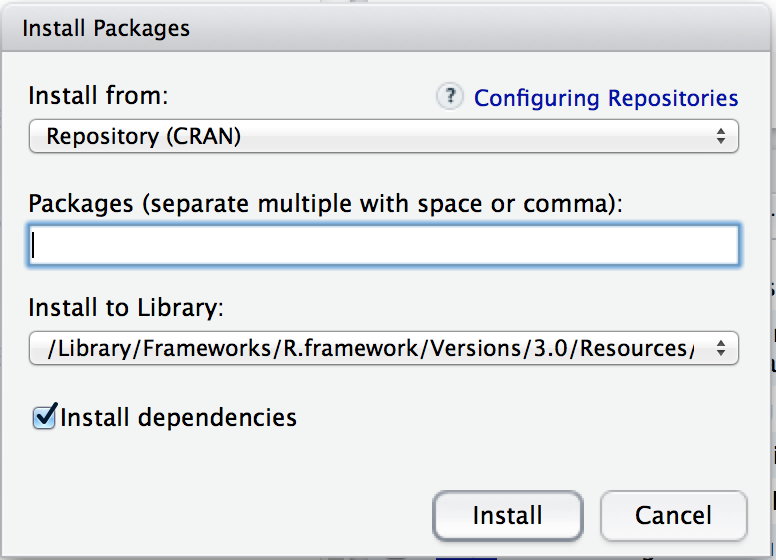
\includegraphics[width=10.78in]{/Users/dave/Documents/GitHub/stats-remix-advanced/bookdown/img/mechanics/installpackage} \caption{The package installation dialog box in RStudio}\label{fig:packageinstalla}
\end{figure}

There are a few different buttons and boxes you can play with. Ignore most of them. Just go to the line that says ``Packages'' and start typing the name of the package that you want. As you type, you'll see a dropdown menu appear (Figure \ref{fig:packageinstallb}), listing names of packages that start with the letters that you've typed so far.

\begin{figure}
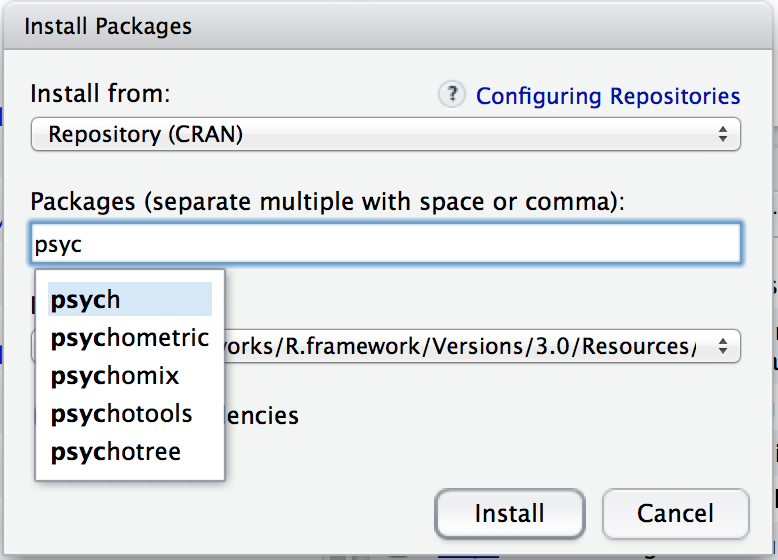
\includegraphics[width=10.81in]{/Users/dave/Documents/GitHub/stats-remix-advanced/bookdown/img/mechanics/installpackage2} \caption{When you start typing, you'll see a dropdown menu suggest a list of possible packages that you might want to install}\label{fig:packageinstallb}
\end{figure}

You can select from this list, or just keep typing. Either way, once you've got the package name that you want, click on the install button at the bottom of the window. When you do, you'll see the following command appear in the R console:

\begin{Shaded}
\begin{Highlighting}[]
\FunctionTok{install.packages}\NormalTok{(}\StringTok{"psych"}\NormalTok{)}
\end{Highlighting}
\end{Shaded}

This is the R command that does all the work. R then goes off to the internet, has a conversation with CRAN, downloads some stuff, and installs it on your computer. You probably don't care about all the details of R's little adventure on the web, but the \texttt{install.packages()} function is rather chatty, so it reports a bunch of gibberish that you really aren't all that interested in:

\begin{verbatim}
trying URL 'http://cran.rstudio.com/bin/macosx/contrib/3.0/psych_1.4.1.tgz'
Content type 'application/x-gzip' length 2737873 bytes (2.6 Mb)
opened URL
==================================================
downloaded 2.6 Mb


The downloaded binary packages are in
    /var/folders/cl/thhsyrz53g73q0w1kb5z3l_80000gn/T//RtmpmQ9VT3/downloaded_packages
\end{verbatim}

Despite the long and tedious response, all thar really means is ``I've installed the psych package''. I find it best to humour the talkative little automaton. I don't actually read any of this garbage, I just politely say ``thanks'' and go back to whatever I was doing.

\hypertarget{updating-r-and-r-packages}{%
\subsection{Updating R and R packages}\label{updating-r-and-r-packages}}

Every now and then the authors of packages release updated versions. The updated versions often add new functionality, fix bugs, and so on. It's generally a good idea to update your packages periodically. There's an \texttt{update.packages()} function that you can use to do this, but it's probably easier to stick with the RStudio tool. In the packages panel, click on the ``Update Packages'' button. This will bring up a window that looks like the one shown in Figure \ref{fig:updatepackages}. In this window, each row refers to a package that needs to be updated. You can to tell R which updates you want to install by checking the boxes on the left. If you're feeling lazy and just want to update everything, click the ``Select All'' button, and then click the ``Install Updates'' button. R then prints out a \emph{lot} of garbage on the screen, individually downloading and installing all the new packages. This might take a while to complete depending on how good your internet connection is. Go make a cup of coffee. Come back, and all will be well.

\begin{figure}
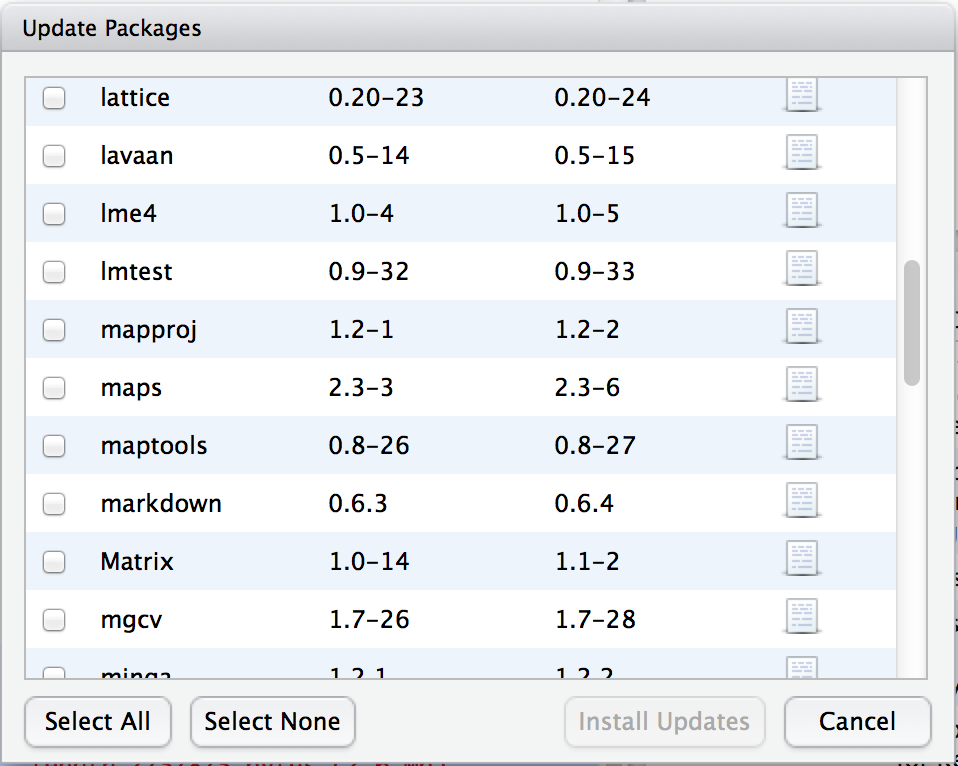
\includegraphics[width=13.31in]{/Users/dave/Documents/GitHub/stats-remix-advanced/bookdown/img/mechanics/updatepackages} \caption{The RStudio dialog box for updating packages}\label{fig:updatepackages}
\end{figure}

About every six months or so, a new version of R is released. You can't update R from within RStudio (not to my knowledge, at least): to get the new version you can go to the CRAN website and download the most recent version of R, and install it in the same way you did when you originally installed R on your computer. This used to be a slightly frustrating event, because whenever you downloaded the new version of R, you would lose all the packages that you'd downloaded and installed, and would have to repeat the process of re-installing them. This was pretty annoying, and there were some neat tricks you could use to get around this. However, newer versions of R don't have this problem so I no longer bother explaining the workarounds for that issue.

\hypertarget{what-packages-does-this-book-use}{%
\subsection{What packages does this book use?}\label{what-packages-does-this-book-use}}

There are several packages that I make use of in this book. The most prominent ones are:

\begin{itemize}
\tightlist
\item
  \texttt{lsr}. This is the \emph{Learning Statistics with R} package that accompanies this book. It doesn't have a lot of interesting high-powered tools: it's just a small collection of handy little things that I think can be useful to novice users. As you get more comfortable with R this package should start to feel pretty useless to you.
\item
  \texttt{psych}. This package, written by William Revelle, includes a lot of tools that are of particular use to psychologists. In particular, there's several functions that are particularly convenient for producing analyses or summaries that are very common in psych, but less common in other disciplines.
\item
  \texttt{car}. This is the \emph{Companion to Applied Regression} package, which accompanies the excellent book of the same name by \citep{Fox2011}. It provides a lot of very powerful tools, only some of which we'll touch in this book.
\end{itemize}

Besides these three, there are a number of packages that I use in a more limited fashion: \texttt{gplots}, \texttt{sciplot}, \texttt{foreign}, \texttt{effects}, \texttt{R.matlab}, \texttt{gdata}, \texttt{lmtest}, and probably one or two others that I've missed. There are also a number of packages that I refer to but don't actually use in this book, such as \texttt{reshape}, \texttt{compute.es}, \texttt{HistData} and \texttt{multcomp} among others. Finally, there are a number of packages that provide more advanced tools that I hope to talk about in future versions of the book, such as \texttt{sem}, \texttt{ez}, \texttt{nlme} and \texttt{lme4}. In any case, whenever I'm using a function that isn't in the core packages, I'll make sure to note this in the text.

\hypertarget{workspace}{%
\section{Managing the workspace}\label{workspace}}

Let's suppose that you're reading through this book, and what you're doing is sitting down with it once a week and working through a whole chapter in each sitting. Not only that, you've been following my advice and typing in all these commands into R. So far during this chapter, you'd have typed quite a few commands, although the only ones that actually involved creating variables were the ones you typed during Section \ref{comments}. As a result, you currently have three variables; \texttt{seeker}, \texttt{lover}, and \texttt{keeper}. These three variables are the contents of your \textbf{\emph{workspace}}, also referred to as the \textbf{global environment}. The workspace is a key concept in R, so in this section we'll talk a lot about what it is and how to manage its contents.

\hypertarget{listing-the-contents-of-the-workspace}{%
\subsection{Listing the contents of the workspace}\label{listing-the-contents-of-the-workspace}}

\begin{figure}
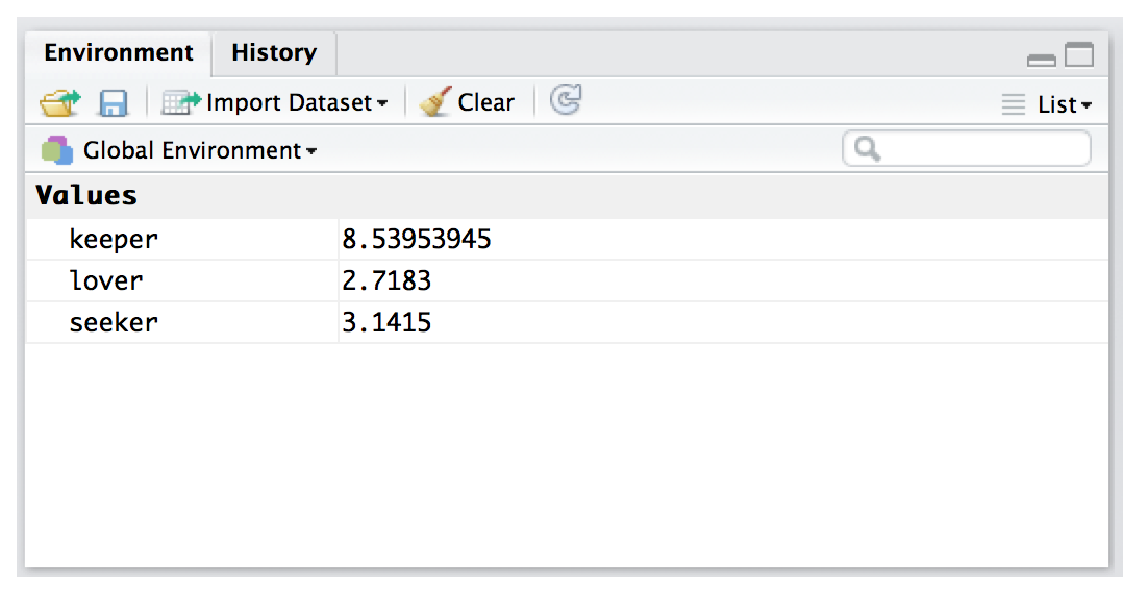
\includegraphics[width=14.75in]{/Users/dave/Documents/GitHub/stats-remix-advanced/bookdown/img/mechanics/workspacepanel} \caption{The RStudio Environment panel shows you the contents of the workspace. The view shown above is the list view. To switch to the grid view, click on the menu item on the top right that currently reads list. Select grid from the dropdown menu, and then it will switch to a view like the one shown in the other workspace figure}\label{fig:workspace}
\end{figure}

\begin{figure}
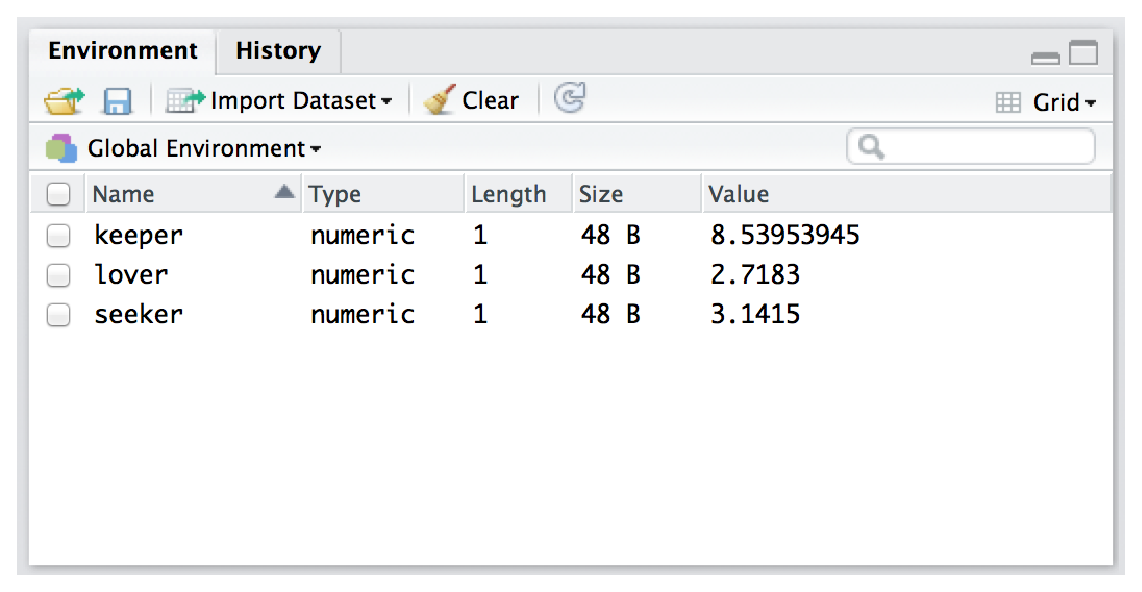
\includegraphics[width=14.78in]{/Users/dave/Documents/GitHub/stats-remix-advanced/bookdown/img/mechanics/workspacepanel2} \caption{The RStudio "Environment" panel shows you the contents of the workspace. Compare this "grid" view to the "list" earlier}\label{fig:workspace2}
\end{figure}

The first thing that you need to know how to do is examine the contents of the workspace. If you're using RStudio, you will probably find that the easiest way to do this is to use the ``Environment'' panel in the top right hand corner. Click on that, and you'll see a list that looks very much like the one shown in Figures \ref{fig:workspace} and \ref{fig:workspace2}. If you're using the commmand line, then the \texttt{objects()} function may come in handy:

\begin{Shaded}
\begin{Highlighting}[]
\FunctionTok{objects}\NormalTok{()}
\end{Highlighting}
\end{Shaded}

\begin{verbatim}
##  [1] "any.sales.this.month" "berkeley"             "berkeley.small"      
##  [4] "coef"                 "days.per.month"       "february.sales"      
##  [7] "greeting"             "is.the.Party.correct" "keeper"              
## [10] "lover"                "months"               "profit"              
## [13] "projecthome"          "revenue"              "royalty"             
## [16] "sales"                "sales.by.month"       "seeker"              
## [19] "simpson"              "stock.levels"         "x"                   
## [22] "xlu"
\end{verbatim}

Of course, in the true R tradition, the \texttt{objects()} function has a lot of fancy capabilities that I'm glossing over in this example. Moreover there are also several other functions that you can use, including \texttt{ls()} which is pretty much identical to \texttt{objects()}, and \texttt{ls.str()} which you can use to get a fairly detailed description of all the variables in the workspace. In fact, the \texttt{lsr} package actually includes its own function that you can use for this purpose, called \texttt{who()}. The reason for using the \texttt{who()} function is pretty straightforward: in my everyday work I find that the output produced by the \texttt{objects()} command isn't \emph{quite} informative enough, because the only thing it prints out is the name of each variable; but the \texttt{ls.str()} function is \emph{too} informative, because it prints out a lot of additional information that I really don't like to look at. The \texttt{who()} function is a compromise between the two. First, now that we've got the \texttt{lsr} package installed, we need to load it:

\begin{Shaded}
\begin{Highlighting}[]
\FunctionTok{library}\NormalTok{(lsr)}
\end{Highlighting}
\end{Shaded}

and now we can use the \texttt{who()} function:

\begin{Shaded}
\begin{Highlighting}[]
\FunctionTok{who}\NormalTok{()}
\end{Highlighting}
\end{Shaded}

\begin{verbatim}
##    -- Name --             -- Class --   -- Size --
##    any.sales.this.month   logical       12        
##    berkeley               data.frame    39 x 3    
##    berkeley.small         data.frame    46 x 2    
##    coef                   numeric       2         
##    days.per.month         numeric       12        
##    february.sales         numeric       1         
##    greeting               character     1         
##    is.the.Party.correct   logical       1         
##    keeper                 numeric       1         
##    lover                  numeric       1         
##    months                 character     12        
##    profit                 numeric       12        
##    projecthome            character     1         
##    revenue                numeric       1         
##    royalty                numeric       1         
##    sales                  numeric       1         
##    sales.by.month         numeric       12        
##    seeker                 numeric       1         
##    simpson                matrix        6 x 5     
##    stock.levels           character     12        
##    x                      logical       3         
##    xlu                    numeric       1
\end{verbatim}

As you can see, the \texttt{who()} function lists all the variables and provides some basic information about what kind of variable each one is and how many elements it contains. Personally, I find this output much easier more useful than the very compact output of the \texttt{objects()} function, but less overwhelming than the extremely verbose \texttt{ls.str()} function. Throughout this book you'll see me using the \texttt{who()} function a lot. You don't have to use it yourself: in fact, I suspect you'll find it easier to look at the RStudio environment panel. But for the purposes of writing a textbook I found it handy to have a nice text based description: otherwise there would be about another 100 or so screenshots added to the book.\footnote{This would be especially annoying if you're reading an electronic copy of the book because the text displayed by the \texttt{who()} function is searchable, whereas text shown in a screen shot isn't!}

\hypertarget{removing-variables-from-the-workspace}{%
\subsection{Removing variables from the workspace}\label{removing-variables-from-the-workspace}}

Looking over that list of variables, it occurs to me that I really don't need them any more. I created them originally just to make a point, but they don't serve any useful purpose anymore, and now I want to get rid of them. I'll show you how to do this, but first I want to warn you -- there's no ``undo'' option for variable removal. Once a variable is removed, it's gone forever unless you save it to disk. I'll show you how to do \emph{that} in Section \ref{load}, but quite clearly we have no need for these variables at all, so we can safely get rid of them.

In RStudio, the easiest way to remove variables is to use the environment panel. Assuming that you're in grid view (i.e., Figure \ref{fig:workspace2}), check the boxes next to the variables that you want to delete, then click on the ``Clear'' button at the top of the panel. When you do this, RStudio will show a dialog box asking you to confirm that you really do want to delete the variables. It's always worth checking that you really do, because as RStudio is at pains to point out, you can't undo this. Once a variable is deleted, it's gone.\footnote{Mind you, all that means is that it's been removed from the workspace. If you've got the data saved to file somewhere, then that \emph{file} is perfectly safe.} In any case, if you click ``yes'', that variable will disappear from the workspace: it will no longer appear in the environment panel, and it won't show up when you use the \texttt{who()} command.

Suppose you don't access to RStudio, and you still want to remove variables. This is where the \textbf{\emph{remove}} function \texttt{rm()} comes in handy. The simplest way to use \texttt{rm()} is just to type in a (comma separated) list of all the variables you want to remove. Let's say I want to get rid of \texttt{seeker} and \texttt{lover}, but I would like to keep \texttt{keeper}. To do this, all I have to do is type:

\begin{Shaded}
\begin{Highlighting}[]
\FunctionTok{rm}\NormalTok{( seeker, lover )}
\end{Highlighting}
\end{Shaded}

There's no visible output, but if I now inspect the workspace

\begin{Shaded}
\begin{Highlighting}[]
\FunctionTok{who}\NormalTok{()}
\end{Highlighting}
\end{Shaded}

\begin{verbatim}
##    -- Name --             -- Class --   -- Size --
##    any.sales.this.month   logical       12        
##    berkeley               data.frame    39 x 3    
##    berkeley.small         data.frame    46 x 2    
##    coef                   numeric       2         
##    days.per.month         numeric       12        
##    february.sales         numeric       1         
##    greeting               character     1         
##    is.the.Party.correct   logical       1         
##    keeper                 numeric       1         
##    months                 character     12        
##    profit                 numeric       12        
##    projecthome            character     1         
##    revenue                numeric       1         
##    royalty                numeric       1         
##    sales                  numeric       1         
##    sales.by.month         numeric       12        
##    simpson                matrix        6 x 5     
##    stock.levels           character     12        
##    x                      logical       3         
##    xlu                    numeric       1
\end{verbatim}

I see that there's only the \texttt{keeper} variable left. As you can see, \texttt{rm()} can be very handy for keeping the workspace tidy.

\hypertarget{navigation}{%
\section{Navigating the file system}\label{navigation}}

In this section I talk a little about how R interacts with the file system on your computer. It's not a terribly interesting topic, but it's useful. As background to this discussion, I'll talk a bit about how file system locations work in Section \ref{filesystem}. Once upon a time \emph{everyone} who used computers could safely be assumed to understand how the file system worked, because it was impossible to successfully use a computer if you didn't! However, modern operating systems are much more ``user friendly'', and as a consequence of this they go to great lengths to hide the file system from users. So these days it's not at all uncommon for people to have used computers most of their life and not be familiar with the way that computers organise files. If you already know this stuff, skip straight to Section \ref{navigationR}. Otherwise, read on. I'll try to give a brief introduction that will be useful for those of you who have never been forced to learn how to navigate around a computer using a DOS or UNIX shell.

\hypertarget{filesystem}{%
\subsection{The file system itself}\label{filesystem}}

In this section I describe the basic idea behind file locations and file paths. Regardless of whether you're using Window, Mac OS or Linux, every file on the computer is assigned a (fairly) human readable address, and every address has the same basic structure: it describes a \emph{path} that starts from a \emph{root} location , through as series of \emph{folders} (or if you're an old-school computer user, \emph{directories}), and finally ends up at the file.

On a Windows computer the root is the physical drive\footnote{Well, the partition, technically.} on which the file is stored, and for most home computers the name of the hard drive that stores all your files is C: and therefore most file names on Windows begin with C:. After that comes the folders, and on Windows the folder names are separated by a \texttt{\textbackslash{}} symbol. So, the complete path to this book on my Windows computer might be something like this:

\begin{verbatim}
C:\Users\danRbook\LSR.pdf
\end{verbatim}

and what that \emph{means} is that the book is called LSR.pdf, and it's in a folder called \texttt{book} which itself is in a folder called dan which itself is \ldots{} well, you get the idea. On Linux, Unix and Mac OS systems, the addresses look a little different, but they're more or less identical in spirit. Instead of using the backslash, folders are separated using a forward slash, and unlike Windows, they don't treat the physical drive as being the root of the file system. So, the path to this book on my Mac might be something like this:

\begin{verbatim}
/Users/dan/Rbook/LSR.pdf
\end{verbatim}

So that's what we mean by the ``path'' to a file. The next concept to grasp is the idea of a \textbf{\emph{working directory}} and how to change it. For those of you who have used command line interfaces previously, this should be obvious already. But if not, here's what I mean. The working directory is just ``whatever folder I'm currently looking at''. Suppose that I'm currently looking for files in Explorer (if you're using Windows) or using Finder (on a Mac). The folder I currently have open is my user directory (i.e., \texttt{C:\textbackslash{}Users\textbackslash{}dan} or \texttt{/Users/dan}). That's my current working directory.

The fact that we can imagine that the program is ``in'' a particular directory means that we can talk about moving \emph{from} our current location \emph{to} a new one. What that means is that we might want to specify a new location in relation to our current location. To do so, we need to introduce two new conventions. Regardless of what operating system you're using, we use \texttt{.} to refer to the current working directory, and \texttt{..} to refer to the directory above it. This allows us to specify a path to a new location in relation to our current location, as the following examples illustrate. Let's assume that I'm using my Windows computer, and my working directory is \texttt{C:\textbackslash{}Users\textbackslash{}danRbook}). The table below shows several addresses in relation to my current one:

\begin{table}

\caption{\label{tab:unnamed-chunk-109}Basic arithmetic operations in R. These five operators are used very frequently throughout the text, so it's important to be familiar with them at the outset.}
\centering
\begin{tabular}[t]{ll}
\toprule
absolute path (i.e., from root) & relative path (i.e. from C:\textbackslash{}Users\textbackslash{}danRbook)\\
\midrule
C:\textbackslash{}\textbackslash{}Users\textbackslash{}\textbackslash{}dan & ..\\
C:\textbackslash{}\textbackslash{}Users & ..\textbackslash{}\textbackslash{}.. \textbackslash{}\textbackslash{}\\
C:\textbackslash{}\textbackslash{}Users\textbackslash{}\textbackslash{}danRbook\textbackslash{}\textbackslash{}source & .\textbackslash{}\textbackslash{}source\\
C:\textbackslash{}\textbackslash{}Users\textbackslash{}\textbackslash{}dan\textbackslash{}\textbackslash{}nerdstuff & ..\textbackslash{}\textbackslash{}nerdstuff\\
\bottomrule
\end{tabular}
\end{table}

There's one last thing I want to call attention to: the \texttt{\textasciitilde{}} directory. I normally wouldn't bother, but R makes reference to this concept sometimes. It's quite common on computers that have multiple users to define \texttt{\textasciitilde{}} to be the user's home directory. On my Mac, for instance, the home directory \texttt{\textasciitilde{}} for the ``dan'' user is \texttt{\textbackslash{}Users\textbackslash{}dan\textbackslash{}}. And so, not surprisingly, it is possible to define other directories in terms of their relationship to the home directory. For example, an alternative way to describe the location of the \texttt{LSR.pdf} file on my Mac would be

\begin{verbatim}
~Rbook\LSR.pdf
\end{verbatim}

That's about all you really need to know about file paths. And since this section already feels too long, it's time to look at how to navigate the file system in R.

\hypertarget{navigationR}{%
\subsection{Navigating the file system using the R console}\label{navigationR}}

In this section I'll talk about how to navigate this file system from within R itself. It's not particularly user friendly, and so you'll probably be happy to know that RStudio provides you with an easier method, and I will describe it in Section \ref{nav3}. So in practice, you won't \emph{really} need to use the commands that I babble on about in this section, but I do think it helps to see them in operation at least once before forgetting about them forever.

Okay, let's get started. When you want to load or save a file in R it's important to know what the working directory is. You can find out by using the \texttt{getwd()} command. For the moment, let's assume that I'm using Mac OS or Linux, since there's some subtleties to Windows. Here's what happens:

\begin{verbatim}
getwd()
## [1] "/Users/dan"
\end{verbatim}

We can change the working directory quite easily using \texttt{setwd()}. The \texttt{setwd()} function has only the one argument, \texttt{dir}, is a character string specifying a path to a directory, or a path relative to the working directory. Since I'm currently located at \texttt{/Users/dan}, the following two are equivalent:

\begin{verbatim}
setwd("/Users/dan/Rbook/data")
setwd("./Rbook/data")
\end{verbatim}

Now that we're here, we can type \texttt{list.files()} command to get a listing of all the files in that directory. Since this is the directory in which I store all of the data files that we'll use in this book, here's what we get as the result:

\begin{verbatim}
list.files()
## [1] "afl24.Rdata"             "aflsmall.Rdata"          "aflsmall2.Rdata"        
## [4] "agpp.Rdata"              "all.zip"                 "annoying.Rdata"         
## [7] "anscombesquartet.Rdata"  "awesome.Rdata"           "awesome2.Rdata"         
## [10] "booksales.csv"           "booksales.Rdata"         "booksales2.csv"         
## [13] "cakes.Rdata"             "cards.Rdata"             "chapek9.Rdata"          
## [16] "chico.Rdata"             "clinicaltrial_old.Rdata" "clinicaltrial.Rdata"    
## [19] "coffee.Rdata"            "drugs.wmc.rt.Rdata"      "dwr_all.Rdata"          
## [22] "effort.Rdata"            "happy.Rdata"             "harpo.Rdata"            
## [25] "harpo2.Rdata"            "likert.Rdata"            "nightgarden.Rdata"      
## [28] "nightgarden2.Rdata"      "parenthood.Rdata"        "parenthood2.Rdata"      
## [31] "randomness.Rdata"        "repeated.Rdata"          "rtfm.Rdata"             
## [34] "salem.Rdata"             "zeppo.Rdata"
\end{verbatim}

Not terribly exciting, I'll admit, but it's useful to know about. In any case, there's only one more thing I want to make a note of, which is that R also makes use of the home directory. You can find out what it is by using the \texttt{path.expand()} function, like this:

\begin{verbatim}
path.expand("~")
## [1] "/Users/dan"
\end{verbatim}

You can change the user directory if you want, but we're not going to make use of it very much so there's no reason to. The only reason I'm even bothering to mention it at all is that when you use RStudio to open a file, you'll see output on screen that defines the path to the file relative to the \texttt{\textasciitilde{}} directory. I'd prefer you not to be confused when you see it.\footnote{One additional thing worth calling your attention to is the \texttt{file.choose()} function. Suppose you want to load a file and you don't quite remember where it is, but would like to browse for it. Typing \texttt{file.choose()} at the command line will open a window in which you can browse to find the file; when you click on the file you want, R will print out the full path to that file. This is kind of handy.}

\hypertarget{why-do-the-windows-paths-use-the-wrong-slash}{%
\subsection{Why do the Windows paths use the wrong slash?}\label{why-do-the-windows-paths-use-the-wrong-slash}}

Let's suppose I'm on Windows. As before, I can find out what my current working directory is like this:

\begin{verbatim}
getwd()
## [1] "C:/Users/dan/
\end{verbatim}

This seems about right, but you might be wondering why R is displaying a Windows path using the wrong type of slash. The answer is slightly complicated, and has to do with the fact that R treats the \texttt{\textbackslash{}} character as ``special'' (see Section \ref{escapechars}). If you're deeply wedded to the idea of specifying a path using the Windows style slashes, then what you need to do is to type \texttt{/} whenever you mean \texttt{\textbackslash{}}. In other words, if you want to specify the working directory on a Windows computer, you need to use one of the following commands:

\begin{verbatim}
setwd( "C:/Users/dan" )
setwd( "C:\\Users\\dan" )
\end{verbatim}

It's kind of annoying to have to do it this way, but as you'll see later on in Section \ref{escapechars} it's a necessary evil. Fortunately, as we'll see in the next section, RStudio provides a much simpler way of changing directories\ldots{}

\hypertarget{nav3}{%
\subsection{Navigating the file system using the RStudio file panel}\label{nav3}}

Although I think it's important to understand how all this command line stuff works, in many (maybe even most) situations there's an easier way. For our purposes, the easiest way to navigate the file system is to make use of RStudio's built in tools. The ``file'' panel -- the lower right hand area in Figure \ref{fig:filepanel} -- is actually a pretty decent file browser. Not only can you just point and click on the names to move around the file system, you can also use it to set the working directory, and even load files.

\begin{figure}
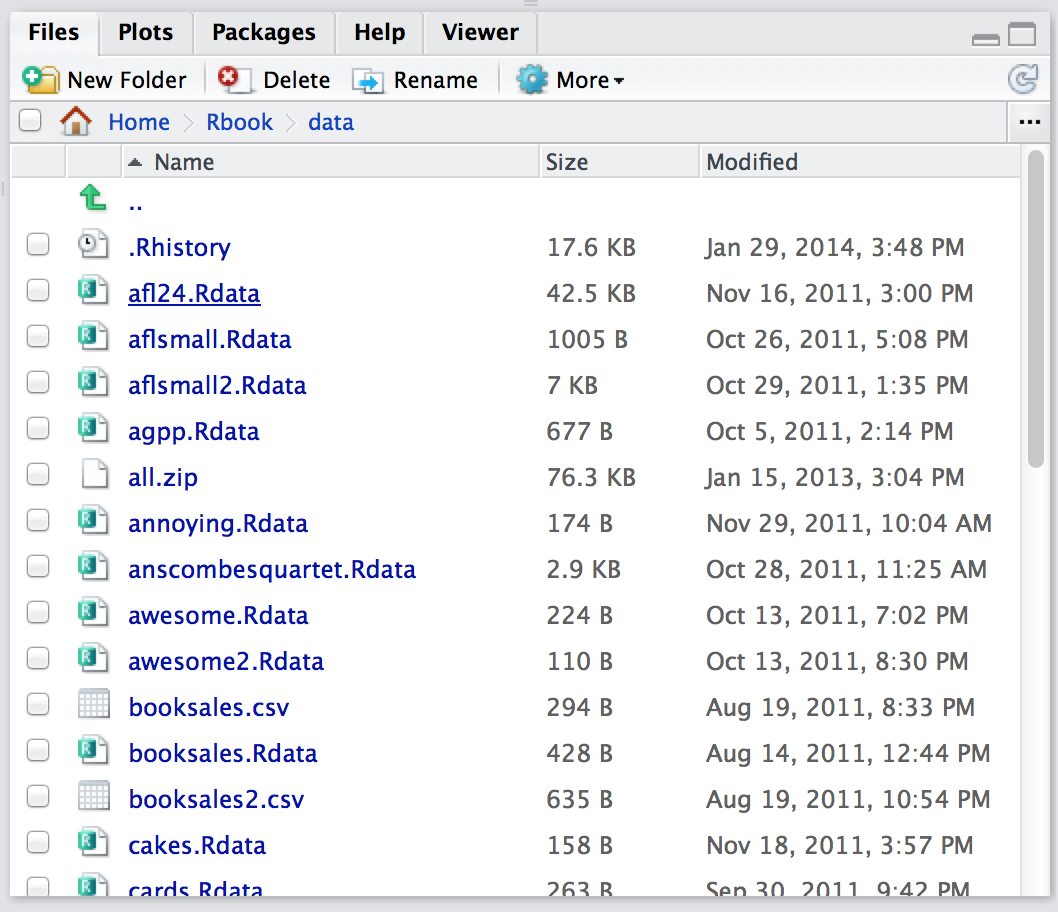
\includegraphics[width=14.69in]{/Users/dave/Documents/GitHub/stats-remix-advanced/bookdown/img/mechanics/filepanel} \caption{The "file panel" is the area shown in the lower right hand corner. It provides a very easy way to browse and navigate your computer using R. See main text for details.}\label{fig:filepanel}
\end{figure}

Here's what you need to do to change the working directory using the file panel. Let's say I'm looking at the actual screen shown in Figure \ref{fig:filepanel}. At the top of the file panel you see some text that says ``Home \(>\) Rbook \(>\) data''. What that means is that it's \emph{displaying} the files that are stored in the

\begin{verbatim}
/Users/dan/Rbook/data
\end{verbatim}

directory on my computer. It does \emph{not} mean that this is the R working directory. If you want to change the R working directory, using the file panel, you need to click on the button that reads ``More''. This will bring up a little menu, and one of the options will be ``Set as Working Directory''. If you select that option, then R really will change the working directory. You can tell that it has done so because this command appears in the console:

\begin{verbatim}
setwd("~/Rbook/data")
\end{verbatim}

In other words, RStudio sends a command to the R console, exactly as if you'd typed it yourself. The file panel can be used to do other things too. If you want to move ``up'' to the parent folder (e.g., from \texttt{/Users/dan/Rbook/data} to \texttt{/Users/dan/Rbook} click on the ``..'' link in the file panel. To move to a subfolder, click on the name of the folder that you want to open. You can open some types of file by clicking on them. You can delete files from your computer using the ``delete'' button, rename them with the ``rename'' button, and so on.

As you can tell, the file panel is a very handy little tool for navigating the file system. But it can do more than just navigate. As we'll see later, it can be used to open files. And if you look at the buttons and menu options that it presents, you can even use it to rename, delete, copy or move files, and create new folders. However, since most of that functionality isn't critical to the basic goals of this book, I'll let you discover those on your own.

\hypertarget{load}{%
\section{Loading and saving data}\label{load}}

There are several different types of files that are likely to be relevant to us when doing data analysis. There are three in particular that are especially important from the perspective of this book:

\begin{itemize}
\tightlist
\item
  \emph{Workspace files} are those with a .Rdata file extension. This is the standard kind of file that R uses to store data and variables. They're called ``workspace files'' because you can use them to save your whole workspace.
\item
  \emph{Comma separated value (CSV) files} are those with a .csv file extension. These are just regular old text files, and they can be opened with almost any software. It's quite typical for people to store data in CSV files, precisely because they're so simple.
\item
  \emph{Script files} are those with a .R file extension. These aren't data files at all; rather, they're used to save a collection of commands that you want R to execute later. They're just text files, but we won't make use of them until Chapter \ref{scripting}.
\end{itemize}

There are also several other types of file that R makes use of,\footnote{Notably those with .rda, .Rd, .Rhistory, .rdb and .rdx extensions} but they're not really all that central to our interests. There are also several other kinds of data file that you might want to import into R. For instance, you might want to open Microsoft Excel spreadsheets (.xlsx files), or data files that have been saved in the native file formats for other statistics software, such as SPSS, SAS, Minitab, Stata or Systat. Finally, you might have to handle databases. R tries hard to play nicely with other software, so it has tools that let you open and work with any of these and many others. I'll discuss some of these other possibilities elsewhere in this book (Section \ref{importing}), but for now I want to focus primarily on the two kinds of data file that you're most likely to need: .Rdata files and .csv files.
In this section I'll talk about how to load a workspace file, how to import data from a CSV file, and how to save your workspace to a workspace file. Throughout this section I'll first describe the (sometimes awkward) R commands that do all the work, and then I'll show you the (much easier) way to do it using RStudio.

\hypertarget{loading-workspace-files-using-r}{%
\subsection{Loading workspace files using R}\label{loading-workspace-files-using-r}}

When I used the \texttt{list.files()} command to list the contents of the \texttt{/Users/dan/Rbook/data} directory (in Section \ref{navigationR}), the output referred to a file called booksales.Rdata. Let's say I want to load the data from this file into my workspace. The way I do this is with the \texttt{load()} function. There are two arguments to this function, but the only one we're interested in is

\begin{itemize}
\tightlist
\item
  \texttt{file}. This should be a character string that specifies a path to the file that needs to be loaded. You can use an absolute path or a relative path to do so.
\end{itemize}

Using the absolute file path, the command would look like this:

\begin{verbatim}
load( file = "/Users/dan/Rbook/data/booksales.Rdata" )
\end{verbatim}

but this is pretty lengthy. Given that the working directory (remember, we changed the directory at the end of Section \ref{nav3}) is \texttt{/Users/dan/Rbook/data}, I could use a relative file path, like so:

\begin{verbatim}
load( file = "../data/booksales.Rdata" )
\end{verbatim}

However, my preference is usually to change the working directory first, and \emph{then} load the file. What that would look like is this:

\begin{verbatim}
setwd( "../data" )         # move to the data directory
load( "booksales.Rdata" )  # load the data
\end{verbatim}

If I were then to type \texttt{who()} I'd see that there are several new variables in my workspace now. Throughout this book, whenever you see me loading a file, I will assume that the file is actually stored in the working directory, or that you've changed the working directory so that R is pointing at the directory that contains the file. Obviously, \emph{you} don't need type that command yourself: you can use the RStudio file panel to do the work.

\hypertarget{loading-workspace-files-using-rstudio}{%
\subsection{Loading workspace files using RStudio}\label{loading-workspace-files-using-rstudio}}

Okay, so how do we open an .Rdata file using the RStudio file panel? It's terribly simple. First, use the file panel to find the folder that contains the file you want to load. If you look at Figure \ref{fig:filepanel}, you can see that there are several .Rdata files listed. Let's say I want to load the \texttt{booksales.Rdata} file. All I have to do is click on the file name. RStudio brings up a little dialog box asking me to confirm that I do want to load this file. I click yes. The following command then turns up in the console,

\begin{verbatim}
load("~/Rbook/data/booksales.Rdata")
\end{verbatim}

and the new variables will appear in the workspace (you'll see them in the Environment panel in RStudio, or if you type \texttt{who()}). So easy it barely warrants having its own section.

\hypertarget{loadingcsv}{%
\subsection{Importing data from CSV files using loadingcsv}\label{loadingcsv}}

One quite commonly used data format is the humble ``comma separated value'' file, also called a CSV file, and usually bearing the file extension .csv. CSV files are just plain old-fashioned text files, and what they store is basically just a table of data. This is illustrated in Figure \ref{fig:booksalescsv}, which shows a file called booksales.csv that I've created. As you can see, each row corresponds to a variable, and each row represents the book sales data for one month. The first row doesn't contain actual data though: it has the names of the variables.

\begin{figure}
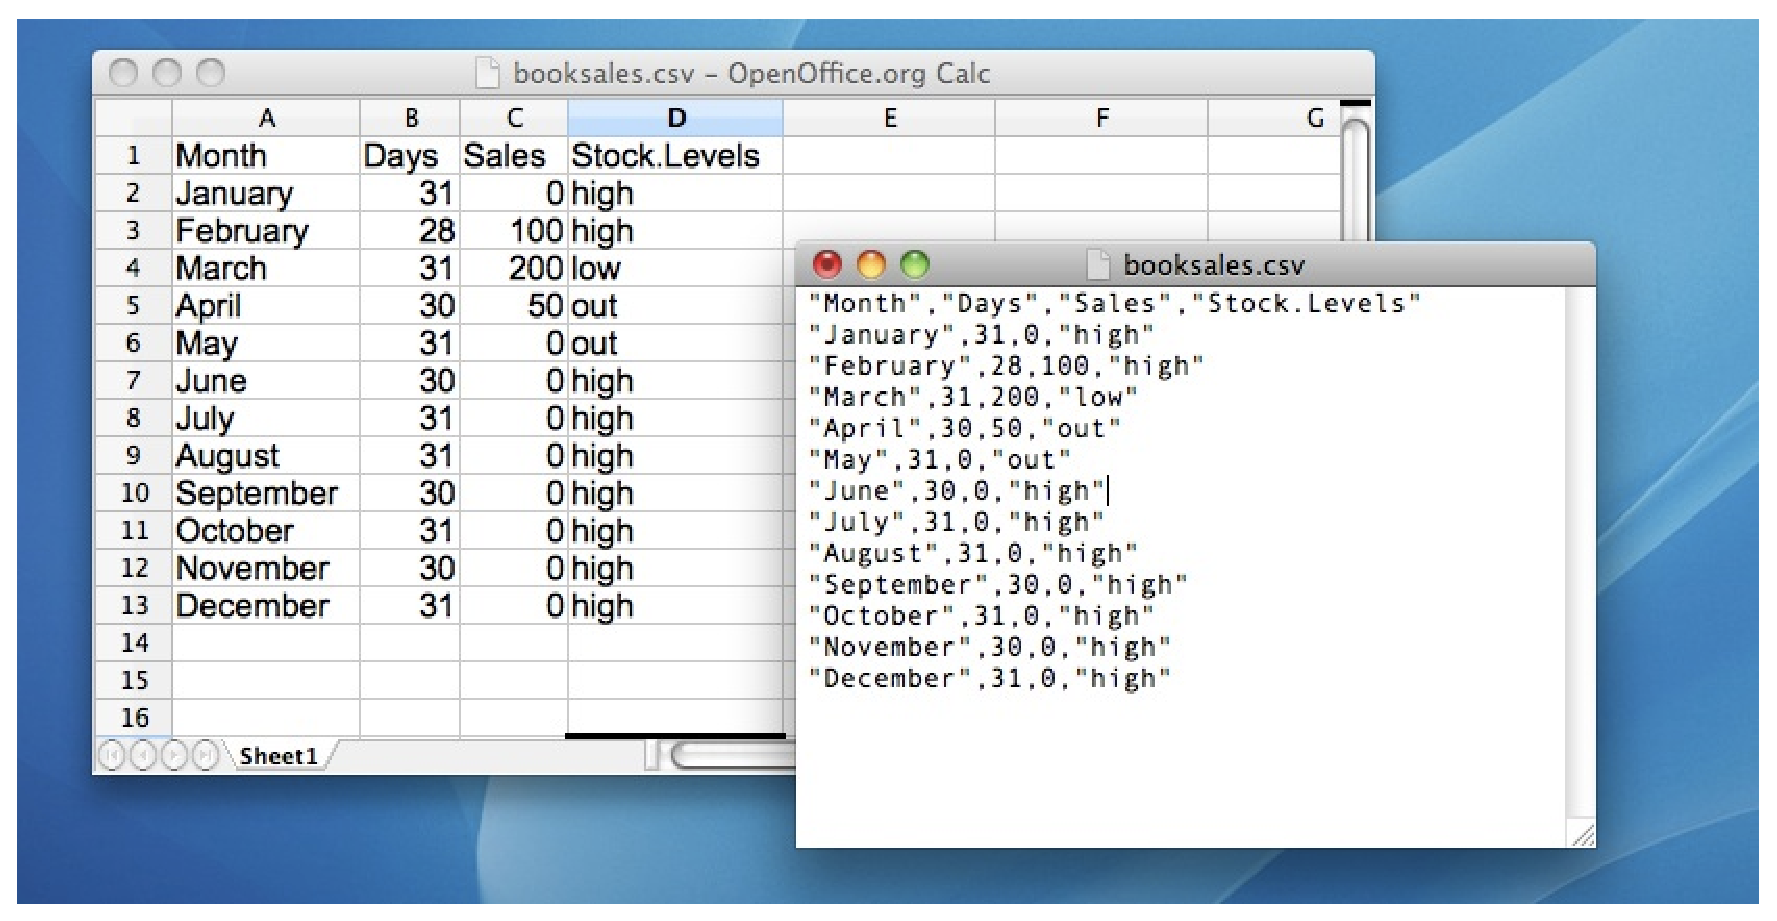
\includegraphics[width=11.61in]{/Users/dave/Documents/GitHub/stats-remix-advanced/bookdown/img/mechanics/booksalescsv} \caption{The booksales.csv data file. On the left, I've opened the file in using a spreadsheet program (OpenOffice), which shows that the file is basically a table. On the right, the same file is open in a standard text editor (the TextEdit program on a Mac), which shows how the file is formatted. The entries in the table are wrapped in quote marks and separated by commas.}\label{fig:booksalescsv}
\end{figure}

If RStudio were not available to you, the easiest way to open this file would be to use the \texttt{read.csv()} function.\footnote{In a lot of books you'll see the \texttt{read.table()} function used for this purpose instead of \texttt{read.csv()}. They're more or less identical functions, with the same arguments and everything. They differ only in the default values.} This function is pretty flexible, and I'll talk a lot more about it's capabilities in Section \ref{importing} for more details, but for now there's only two arguments to the function that I'll mention:

\begin{itemize}
\tightlist
\item
  \texttt{file}. This should be a character string that specifies a path to the file that needs to be loaded. You can use an absolute path or a relative path to do so.
\item
  \texttt{header}. This is a logical value indicating whether or not the first row of the file contains variable names. The default value is \texttt{TRUE}.
\end{itemize}

Therefore, to import the CSV file, the command I need is:

\begin{Shaded}
\begin{Highlighting}[]
\NormalTok{books }\OtherTok{\textless{}{-}} \FunctionTok{read.csv}\NormalTok{( }\AttributeTok{file =} \StringTok{"booksales.csv"}\NormalTok{ )}
\end{Highlighting}
\end{Shaded}

There are two very important points to notice here. Firstly, notice that I \emph{didn't} try to use the \texttt{load()} function, because that function is only meant to be used for .Rdata files. If you try to use \texttt{load()} on other types of data, you get an error. Secondly, notice that when I imported the CSV file I assigned the result to a variable, which I imaginatively called \texttt{books}.\footnote{Note that I didn't to this in my earlier example when loading the .Rdata} file. There's a reason for this. The idea behind an \texttt{.Rdata} file is that it stores a whole workspace. So, if you had the ability to look inside the file yourself you'd see that the data file keeps track of all the variables and their names. So when you \texttt{load()} the file, R restores all those original names. CSV files are treated differently: as far as R is concerned, the CSV only stores \emph{one} variable, but that variable is big table. So when you import that table into the workspace, R expects \emph{you} to give it a name.{]} Let's have a look at what we've got:

\begin{Shaded}
\begin{Highlighting}[]
\FunctionTok{print}\NormalTok{( books )}
\end{Highlighting}
\end{Shaded}

\begin{verbatim}
##        Month Days Sales Stock.Levels
## 1    January   31     0         high
## 2   February   28   100         high
## 3      March   31   200          low
## 4      April   30    50          out
## 5        May   31     0          out
## 6       June   30     0         high
## 7       July   31     0         high
## 8     August   31     0         high
## 9  September   30     0         high
## 10   October   31     0         high
## 11  November   30     0         high
## 12  December   31     0         high
\end{verbatim}

Clearly, it's worked, but the format of this output is a bit unfamiliar. We haven't seen anything like this before. What you're looking at is a \emph{data frame}, which is a very important kind of variable in R, and one I'll discuss in Section \ref{dataframes}. For now, let's just be happy that we imported the data and that it looks about right.

\hypertarget{importing-data-from-csv-files-using-rstudio}{%
\subsection{Importing data from CSV files using RStudio}\label{importing-data-from-csv-files-using-rstudio}}

Yet again, it's easier in RStudio. In the environment panel in RStudio you should see a button called ``Import Dataset''. Click on that, and it will give you a couple of options: select the ``From Text File\ldots{}'' option, and it will open up a very familiar dialog box asking you to select a file: if you're on a Mac, it'll look like the usual Finder window that you use to choose a file; on Windows it looks like an Explorer window. An example of what it looks like on a Mac is shown in Figure \ref{fig:fileopen}. I'm assuming that you're familiar with your own computer, so you should have no problem finding the CSV file that you want to import! Find the one you want, then click on the ``Open'' button. When you do this, you'll see a window that looks like the one in Figure \ref{fig:import}.

\begin{figure}
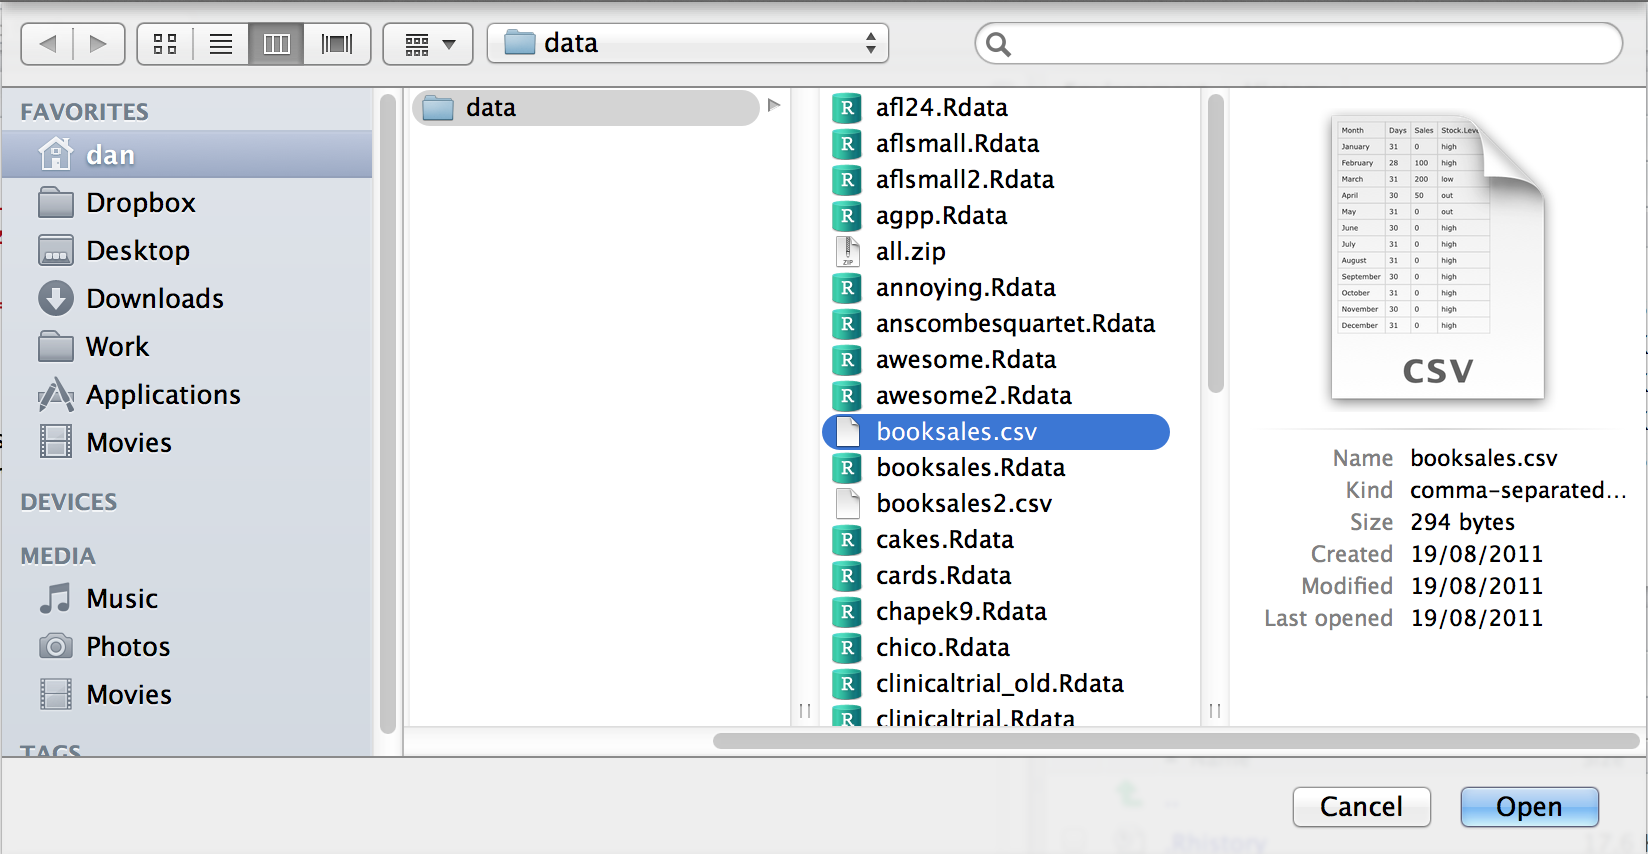
\includegraphics[width=22.89in]{/Users/dave/Documents/GitHub/stats-remix-advanced/bookdown/img/mechanics/openscreen} \caption{A dialog box on a Mac asking you to select the CSV file R should try to import. Mac users will recognise this immediately: it's the usual way in which a Mac asks you to find a file. Windows users won't see this: they'll see the usual explorer window that Windows always gives you when it wants you to select a file.}\label{fig:fileopen}
\end{figure}

The import data set window is relatively straightforward to understand.

\begin{figure}
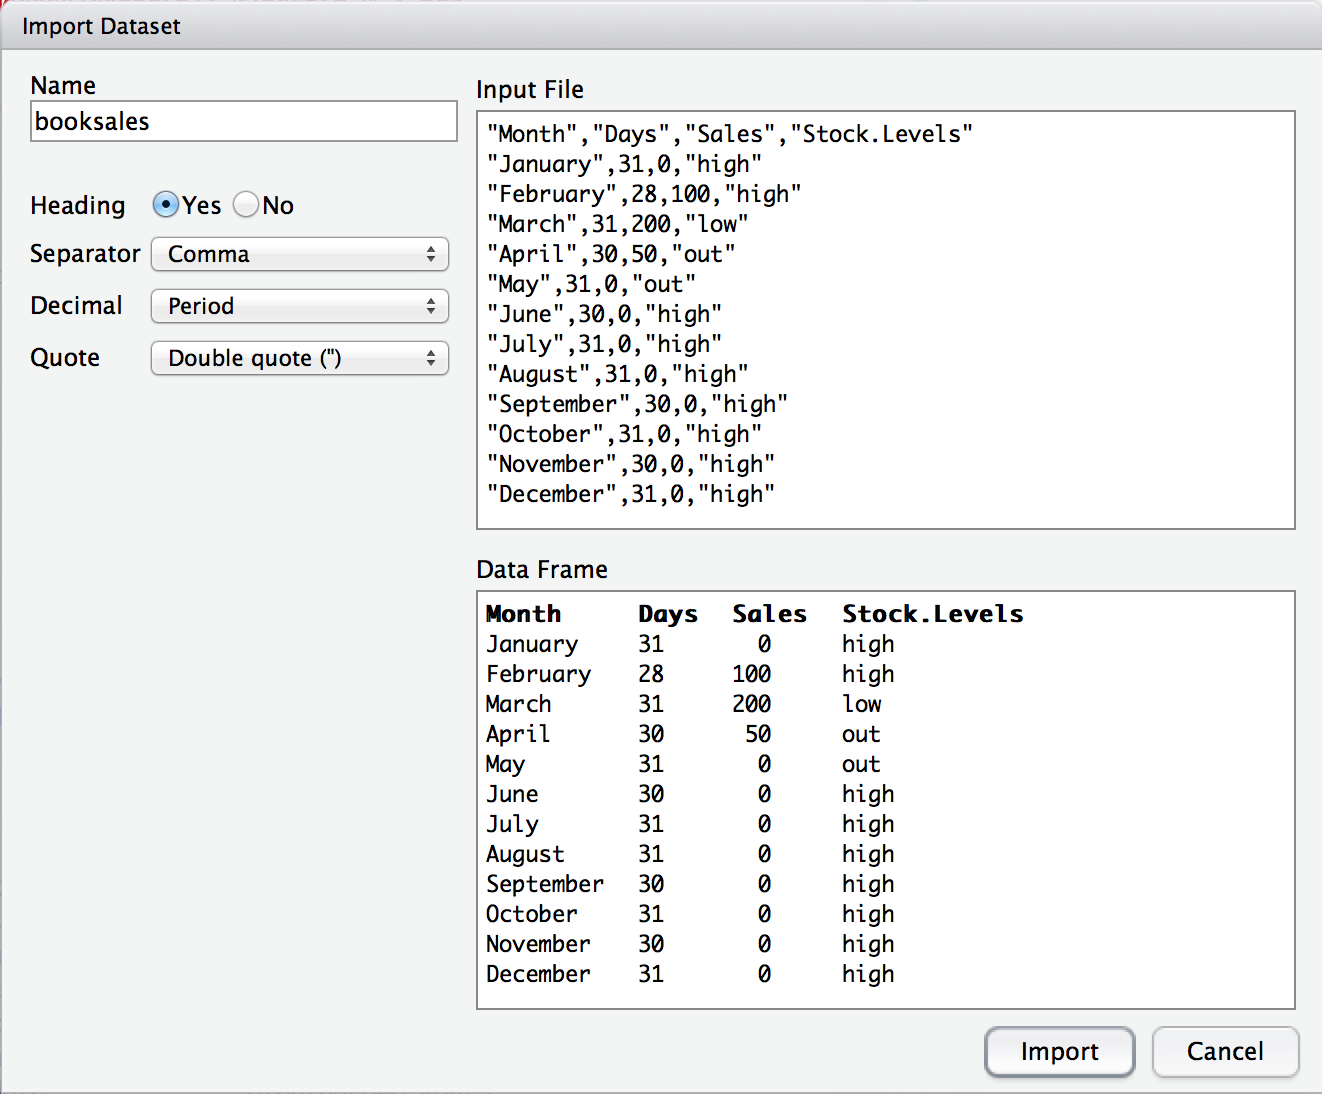
\includegraphics[width=18.36in]{/Users/dave/Documents/GitHub/stats-remix-advanced/bookdown/img/mechanics/import} \caption{The RStudio window for importing a CSV file into R}\label{fig:import}
\end{figure}

In the top left corner, you need to type the name of the variable you R to create. By default, that will be the same as the file name: our file is called \texttt{booksales.csv}, so RStudio suggests the name \texttt{booksales}. If you're happy with that, leave it alone. If not, type something else. Immediately below this are a few things that you can tweak to make sure that the data gets imported correctly:

\begin{itemize}
\tightlist
\item
  Heading. Does the first row of the file contain raw data, or does it contain headings for each variable? The \texttt{booksales.csv} file has a header at the top, so I selected ``yes''.
\item
  Separator. What character is used to separate different entries? In most CSV files this will be a comma (it is ``comma separated'' after all). But you can change this if your file is different.
\item
  Decimal. What character is used to specify the decimal point? In English speaking countries, this is almost always a period (i.e., \texttt{.}). That's not universally true: many European countries use a comma. So you can change that if you need to.
\item
  Quote. What character is used to denote a block of text? That's usually going to be a double quote mark. It is for the \texttt{booksales.csv} file, so that's what I selected.
\end{itemize}

The nice thing about the RStudio window is that it shows you the raw data file at the top of the window, and it shows you a preview of the data at the bottom. If the data at the bottom doesn't look right, try changing some of the settings on the left hand side. Once you're happy, click ``Import''. When you do, two commands appear in the R console:

\begin{verbatim}
booksales <- read.csv("~/Rbook/data/booksales.csv")
View(booksales)
\end{verbatim}

The first of these commands is the one that loads the data. The second one will display a pretty table showing the data in RStudio.

\hypertarget{saving-a-workspace-file-using-save}{%
\subsection{\texorpdfstring{Saving a workspace file using \texttt{save}}{Saving a workspace file using save}}\label{saving-a-workspace-file-using-save}}

Not surprisingly, saving data is very similar to loading data. Although RStudio provides a simple way to save files (see below), it's worth understanding the actual commands involved. There are two commands you can use to do this, \texttt{save()} and \texttt{save.image()}. If you're happy to save \emph{all} of the variables in your workspace into the data file, then you should use \texttt{save.image()}. And if you're happy for R to save the file into the current working directory, all you have to do is this:

\begin{Shaded}
\begin{Highlighting}[]
\FunctionTok{save.image}\NormalTok{( }\AttributeTok{file =} \StringTok{"myfile.Rdata"}\NormalTok{ )}
\end{Highlighting}
\end{Shaded}

Since \texttt{file} is the first argument, you can shorten this to \texttt{save.image("myfile.Rdata")}; and if you want to save to a different directory, then (as always) you need to be more explicit about specifying the path to the file, just as we discussed in Section \ref{navigation}. Suppose, however, I have several variables in my workspace, and I only want to save some of them. For instance, I might have this as my workspace:

\begin{Shaded}
\begin{Highlighting}[]
\FunctionTok{who}\NormalTok{()}
\DocumentationTok{\#\#   {-}{-} Name {-}{-}   {-}{-} Class {-}{-}   {-}{-} Size {-}{-}}
\DocumentationTok{\#\#   data         data.frame    3 x 2     }
\DocumentationTok{\#\#   handy        character     1         }
\DocumentationTok{\#\#   junk         numeric       1        }
\end{Highlighting}
\end{Shaded}

I want to save \texttt{data} and \texttt{handy}, but not \texttt{junk}. But I don't want to delete \texttt{junk} right now, because I want to use it for something else later on. This is where the \texttt{save()} function is useful, since it lets me indicate exactly which variables I want to save. Here is one way I can use the \texttt{save} function to solve my problem:

\begin{Shaded}
\begin{Highlighting}[]
\FunctionTok{save}\NormalTok{(data, handy, }\AttributeTok{file =} \StringTok{"myfile.Rdata"}\NormalTok{)}
\end{Highlighting}
\end{Shaded}

Importantly, you \emph{must} specify the name of the \texttt{file} argument. The reason is that if you don't do so, R will think that \texttt{"myfile.Rdata"} is actually a \emph{variable} that you want to save, and you'll get an error message. Finally, I should mention a second way to specify which variables the \texttt{save()} function should save, which is to use the \texttt{list} argument. You do so like this:

\begin{Shaded}
\begin{Highlighting}[]
\NormalTok{save.me }\OtherTok{\textless{}{-}} \FunctionTok{c}\NormalTok{(}\StringTok{"data"}\NormalTok{, }\StringTok{"handy"}\NormalTok{)   }\CommentTok{\# the variables to be saved}
\FunctionTok{save}\NormalTok{( }\AttributeTok{file =} \StringTok{"booksales2.Rdata"}\NormalTok{, }\AttributeTok{list =}\NormalTok{ save.me )   }\CommentTok{\# the command to save them}
\end{Highlighting}
\end{Shaded}

\hypertarget{save1}{%
\subsection{Saving a workspace file using RStudio}\label{save1}}

RStudio allows you to save the workspace pretty easily. In the environment panel (Figures \ref{fig:workspace} and \ref{fig:workspace2}) you can see the ``save'' button. There's no text, but it's the same icon that gets used on every computer everywhere: it's the one that looks like a floppy disk. You know, those things that haven't been used in about 20 years. Alternatively, go to the ``Session'' menu and click on the ``Save Workspace As\ldots{}'' option.\footnote{A word of warning: what you \emph{don't} want to do is use the ``File'' menu. If you look in the ``File'' menu you will see ``Save'' and ``Save As\ldots{}'' options, but they don't save the workspace. Those options are used for dealing with \emph{scripts}, and so they'll produce \texttt{.R} files. We won't get to those until Chapter \ref{scripting}.} This will bring up the standard ``save'' dialog box for your operating system (e.g., on a Mac it'll look a little bit like the loading dialog box in Figure \ref{fig:fileopen}). Type in the name of the file that you want to save it to, and all the variables in your workspace will be saved to disk. You'll see an R command like this one

\begin{Shaded}
\begin{Highlighting}[]
\FunctionTok{save.image}\NormalTok{(}\StringTok{"\textasciitilde{}/Desktop/Untitled.RData"}\NormalTok{)}
\end{Highlighting}
\end{Shaded}

Pretty straightforward, really.

\hypertarget{other-things-you-might-want-to-save}{%
\subsection{Other things you might want to save}\label{other-things-you-might-want-to-save}}

Until now, we've talked mostly about loading and saving \emph{data}. Other things you might want to save include:

\begin{itemize}
\item
  \emph{The output}. Sometimes you might also want to keep a copy of all your interactions with R, including everything that you typed in and everything that R did in response. There are some functions that you can use to get R to write its output to a file rather than to print onscreen (e.g., \texttt{sink()}), but to be honest, if you do want to save the R output, the easiest thing to do is to use the mouse to select the relevant text in the R console, go to the ``Edit'' menu in RStudio and select ``Copy''. The output has now been copied to the clipboard. Now open up your favourite text editor or word processing software, and paste it. And you're done. However, this will only save the contents of the console, not the plots you've drawn (assuming you've drawn some). We'll talk about saving images later on.
\item
  \emph{A script}. While it is possible -- and sometimes handy -- to save the R output as a method for keeping a copy of your statistical analyses, another option that people use a lot (especially when you move beyond simple ``toy'' analyses) is to write \emph{scripts}. A script is a text file in which you write out all the commands that you want R to run. You can write your script using whatever software you like. In real world data analysis writing scripts is a key skill -- and as you become familiar with R you'll probably find that most of what you do involves scripting rather than typing commands at the R prompt. However, you won't need to do much scripting initially, so we'll leave that until Chapter \ref{scripting}.
\end{itemize}

\hypertarget{useful}{%
\section{Useful things to know about variables}\label{useful}}

In Chapter \ref{introR} I talked a lot about variables, how they're assigned and some of the things you can do with them, but there's a lot of additional complexities. That's not a surprise of course. However, some of those issues are worth drawing your attention to now. So that's the goal of this section; to cover a few extra topics. As a consequence, this section is basically a bunch of things that I want to briefly mention, but don't really fit in anywhere else. In short, I'll talk about several different issues in this section, which are only loosely connected to one another.

\hypertarget{specials}{%
\subsection{Special values}\label{specials}}

The first thing I want to mention are some of the ``special'' values that you might see R produce. Most likely you'll see them in situations where you were expecting a number, but there are quite a few other ways you can encounter them. These values are \texttt{Inf}, \texttt{NaN}, \texttt{NA} and \texttt{NULL}. These values can crop up in various different places, and so it's important to understand what they mean.

\begin{itemize}
\tightlist
\item
  \emph{Infinity} (\texttt{Inf}). The easiest of the special values to explain is \texttt{Inf}, since it corresponds to a value that is infinitely large. You can also have \texttt{-Inf}. The easiest way to get \texttt{Inf} is to divide a positive number by 0:
\end{itemize}

\begin{Shaded}
\begin{Highlighting}[]
\DecValTok{1} \SpecialCharTok{/} \DecValTok{0}
\end{Highlighting}
\end{Shaded}

\begin{verbatim}
## [1] Inf
\end{verbatim}

In most real world data analysis situations, if you're ending up with infinite numbers in your data, then something has gone awry. Hopefully you'll never have to see them.

\begin{itemize}
\tightlist
\item
  \emph{Not a Number} (\texttt{NaN}). The special value of \texttt{NaN} is short for ``not a number'', and it's basically a reserved keyword that means ``there isn't a mathematically defined number for this''. If you can remember your high school maths, remember that it is conventional to say that \(0/0\) doesn't have a proper answer: mathematicians would say that \(0/0\) is \emph{undefined}. R says that it's not a number:
\end{itemize}

\begin{Shaded}
\begin{Highlighting}[]
 \DecValTok{0} \SpecialCharTok{/} \DecValTok{0}
\end{Highlighting}
\end{Shaded}

\begin{verbatim}
## [1] NaN
\end{verbatim}

Nevertheless, it's still treated as a ``numeric'' value. To oversimplify, \texttt{NaN} corresponds to cases where you asked a proper numerical question that genuinely has \emph{no meaningful answer}.

\begin{itemize}
\item
  \emph{Not available} (\texttt{NA}).
  \texttt{NA} indicates that the value that is ``supposed'' to be stored here is missing. To understand what this means, it helps to recognise that the \texttt{NA} value is something that you're most likely to see when analysing data from real world experiments. Sometimes you get equipment failures, or you lose some of the data, or whatever. The point is that some of the information that you were ``expecting'' to get from your study is just plain missing. Note the difference between \texttt{NA} and \texttt{NaN}. For \texttt{NaN}, we really do know what's supposed to be stored; it's just that it happens to correspond to something like \(0/0\) that doesn't make any sense at all. In contrast, \texttt{NA} indicates that we actually don't know what was supposed to be there. The information is \emph{missing}.
\item
  \emph{No value} (\texttt{NULL}).
  The \texttt{NULL} value takes this ``absence'' concept even further. It basically asserts that the variable genuinely has no value whatsoever. This is quite different to both \texttt{NaN} and \texttt{NA}. For \texttt{NaN} we actually know what the value is, because it's something insane like \(0/0\). For \texttt{NA}, we believe that there is supposed to be a value ``out there'', but a dog ate our homework and so we don't quite know what it is. But for \texttt{NULL} we strongly believe that there is \emph{no value at all}.
\end{itemize}

\hypertarget{names}{%
\subsection{Assigning names to vector elements}\label{names}}

One thing that is sometimes a little unsatisfying about the way that R prints out a vector is that the elements come out unlabelled. Here's what I mean. Suppose I've got data reporting the quarterly profits for some company. If I just create a no-frills vector, I have to rely on memory to know which element corresponds to which event. That is:

\begin{Shaded}
\begin{Highlighting}[]
\NormalTok{profit }\OtherTok{\textless{}{-}} \FunctionTok{c}\NormalTok{( }\FloatTok{3.1}\NormalTok{, }\FloatTok{0.1}\NormalTok{, }\SpecialCharTok{{-}}\FloatTok{1.4}\NormalTok{, }\FloatTok{1.1}\NormalTok{ )}
\NormalTok{profit}
\end{Highlighting}
\end{Shaded}

\begin{verbatim}
## [1]  3.1  0.1 -1.4  1.1
\end{verbatim}

You can probably guess that the first element corresponds to the first quarter, the second element to the second quarter, and so on, but that's only because I've told you the back story and because this happens to be a very simple example. In general, it can be quite difficult. This is where it can be helpful to assign \texttt{names} to each of the elements. Here's how you do it:

\begin{Shaded}
\begin{Highlighting}[]
\FunctionTok{names}\NormalTok{(profit) }\OtherTok{\textless{}{-}} \FunctionTok{c}\NormalTok{(}\StringTok{"Q1"}\NormalTok{,}\StringTok{"Q2"}\NormalTok{,}\StringTok{"Q3"}\NormalTok{,}\StringTok{"Q4"}\NormalTok{)}
\NormalTok{profit}
\end{Highlighting}
\end{Shaded}

\begin{verbatim}
##   Q1   Q2   Q3   Q4 
##  3.1  0.1 -1.4  1.1
\end{verbatim}

This is a slightly odd looking command, admittedly, but it's not too difficult to follow. All we're doing is assigning a vector of labels (character strings) to \texttt{names(profit)}. You can always delete the names again by using the command \texttt{names(profit)\ \textless{}-\ NULL}. It's also worth noting that you don't have to do this as a two stage process. You can get the same result with this command:

\begin{Shaded}
\begin{Highlighting}[]
\NormalTok{profit }\OtherTok{\textless{}{-}} \FunctionTok{c}\NormalTok{( }\StringTok{"Q1"} \OtherTok{=} \FloatTok{3.1}\NormalTok{, }\StringTok{"Q2"} \OtherTok{=} \FloatTok{0.1}\NormalTok{, }\StringTok{"Q3"} \OtherTok{=} \SpecialCharTok{{-}}\FloatTok{1.4}\NormalTok{, }\StringTok{"Q4"} \OtherTok{=} \FloatTok{1.1}\NormalTok{ )}
\NormalTok{profit}
\end{Highlighting}
\end{Shaded}

\begin{verbatim}
##   Q1   Q2   Q3   Q4 
##  3.1  0.1 -1.4  1.1
\end{verbatim}

The important things to notice are that (a) this does make things much easier to read, but (b) the names at the top aren't the ``real'' data. The \emph{value} of \texttt{profit{[}1{]}} is still \texttt{3.1}; all I've done is added a \emph{name} to \texttt{profit{[}1{]}} as well. Nevertheless, names aren't purely cosmetic, since R allows you to pull out particular elements of the vector by referring to their names:

\begin{Shaded}
\begin{Highlighting}[]
\NormalTok{profit[}\StringTok{"Q1"}\NormalTok{]}
\end{Highlighting}
\end{Shaded}

\begin{verbatim}
##  Q1 
## 3.1
\end{verbatim}

And if I ever need to pull out the names themselves, then I just type \texttt{names(profit)}.

\hypertarget{variable-classes}{%
\subsection{Variable classes}\label{variable-classes}}

As we've seen, R allows you to store different kinds of data. In particular, the variables we've defined so far have either been character data (text), numeric data, or logical data.\footnote{Or functions. But let's ignore functions for the moment.} It's important that we remember what kind of information each variable stores (and even more important that R remembers) since different kinds of variables allow you to do different things to them. For instance, if your variables have numerical information in them, then it's okay to multiply them together:

\begin{Shaded}
\begin{Highlighting}[]
\NormalTok{x }\OtherTok{\textless{}{-}} \DecValTok{5}   \CommentTok{\# x is numeric}
\NormalTok{y }\OtherTok{\textless{}{-}} \DecValTok{4}   \CommentTok{\# y is numeric}
\NormalTok{x }\SpecialCharTok{*}\NormalTok{ y    }
\end{Highlighting}
\end{Shaded}

\begin{verbatim}
## [1] 20
\end{verbatim}

But if they contain character data, multiplication makes no sense whatsoever, and R will complain if you try to do it:

\begin{Shaded}
\begin{Highlighting}[]
\NormalTok{x }\OtherTok{\textless{}{-}} \StringTok{"apples"}   \CommentTok{\# x is character}
\NormalTok{y }\OtherTok{\textless{}{-}} \StringTok{"oranges"}  \CommentTok{\# y is character}
\NormalTok{x }\SpecialCharTok{*}\NormalTok{ y           }
\end{Highlighting}
\end{Shaded}

\begin{verbatim}
## Error in x * y: non-numeric argument to binary operator
\end{verbatim}

Even R is smart enough to know you can't multiply \texttt{"apples"} by \texttt{"oranges"}. It knows this because the quote marks are indicators that the variable is supposed to be treated as text, not as a number.

This is quite useful, but notice that it means that R makes a big distinction between \texttt{5} and \texttt{"5"}. Without quote marks, R treats \texttt{5} as the number five, and will allow you to do calculations with it. With the quote marks, R treats \texttt{"5"} as the textual character five, and doesn't recognise it as a number any more than it recognises \texttt{"p"} or \texttt{"five"} as numbers. As a consequence, there's a big difference between typing \texttt{x\ \textless{}-\ 5} and typing \texttt{x\ \textless{}-\ "5"}. In the former, we're storing the number \texttt{5}; in the latter, we're storing the character \texttt{"5"}. Thus, if we try to do multiplication with the character versions, R gets stroppy:

\begin{Shaded}
\begin{Highlighting}[]
\NormalTok{x }\OtherTok{\textless{}{-}} \StringTok{"5"}   \CommentTok{\# x is character}
\NormalTok{y }\OtherTok{\textless{}{-}} \StringTok{"4"}   \CommentTok{\# y is character}
\NormalTok{x }\SpecialCharTok{*}\NormalTok{ y     }
\end{Highlighting}
\end{Shaded}

\begin{verbatim}
## Error in x * y: non-numeric argument to binary operator
\end{verbatim}

Okay, let's suppose that I've forgotten what kind of data I stored in the variable \texttt{x} (which happens depressingly often). R provides a function that will let us find out. Or, more precisely, it provides \emph{three} functions: \texttt{class()}, \texttt{mode()} and \texttt{typeof()}. Why the heck does it provide three functions, you might be wondering? Basically, because R actually keeps track of three different kinds of information about a variable:

\begin{enumerate}
\def\labelenumi{\arabic{enumi}.}
\tightlist
\item
  The \textbf{\emph{class}} of a variable is a ``high level'' classification, and it captures psychologically (or statistically) meaningful distinctions. For instance \texttt{"2011-09-12"} and \texttt{"my\ birthday"} are both text strings, but there's an important difference between the two: one of them is a date. So it would be nice if we could get R to recognise that \texttt{"2011-09-12"} is a date, and allow us to do things like add or subtract from it. The class of a variable is what R uses to keep track of things like that. Because the class of a variable is critical for determining what R can or can't do with it, the \texttt{class()} function is very handy.
\item
  The \textbf{\emph{mode}} of a variable refers to the format of the information that the variable stores. It tells you whether R has stored text data or numeric data, for instance, which is kind of useful, but it only makes these ``simple'' distinctions. It can be useful to know about, but it's not the main thing we care about. So I'm not going to use the \texttt{mode()} function very much.\footnote{Actually, I don't think I \emph{ever} use this in practice. I don't know why I bother to talk about it in the book anymore.}
\item
  The \textbf{\emph{type}} of a variable is a very low level classification. We won't use it in this book, but (for those of you that care about these details) this is where you can see the distinction between integer data, double precision numeric, etc. Almost none of you actually will care about this, so I'm not even going to bother demonstrating the \texttt{typeof()} function.
\end{enumerate}

For purposes, it's the \texttt{class()} of the variable that we care most about. Later on, I'll talk a bit about how you can convince R to ``coerce'' a variable to change from one class to another (Section \ref{coercion}). That's a useful skill for real world data analysis, but it's not something that we need right now. In the meantime, the following examples illustrate the use of the \texttt{class()} function:

\begin{Shaded}
\begin{Highlighting}[]
\NormalTok{x }\OtherTok{\textless{}{-}} \StringTok{"hello world"}     \CommentTok{\# x is text}
\FunctionTok{class}\NormalTok{(x)}
\end{Highlighting}
\end{Shaded}

\begin{verbatim}
## [1] "character"
\end{verbatim}

\begin{Shaded}
\begin{Highlighting}[]
\NormalTok{x }\OtherTok{\textless{}{-}} \ConstantTok{TRUE}     \CommentTok{\# x is logical }
\FunctionTok{class}\NormalTok{(x)}
\end{Highlighting}
\end{Shaded}

\begin{verbatim}
## [1] "logical"
\end{verbatim}

\begin{Shaded}
\begin{Highlighting}[]
\NormalTok{x }\OtherTok{\textless{}{-}} \DecValTok{100}     \CommentTok{\# x is a number}
\FunctionTok{class}\NormalTok{(x)}
\end{Highlighting}
\end{Shaded}

\begin{verbatim}
## [1] "numeric"
\end{verbatim}

Exciting, no?

\hypertarget{factors}{%
\section{Factors}\label{factors}}

Okay, it's time to start introducing some of the data types that are somewhat more specific to statistics. If you remember back to Chapter \ref{studydesign}, when we assign numbers to possible outcomes, these numbers can mean quite different things depending on what kind of variable we are attempting to measure. In particular, we commonly make the distinction between \emph{nominal}, \emph{ordinal}, \emph{interval} and \emph{ratio} scale data. How do we capture this distinction in R? Currently, we only seem to have a single numeric data type. That's probably not going to be enough, is it?

A little thought suggests that the numeric variable class in R is perfectly suited for capturing ratio scale data. For instance, if I were to measure response time (RT) for five different events, I could store the data in R like this:

\begin{Shaded}
\begin{Highlighting}[]
\NormalTok{RT }\OtherTok{\textless{}{-}} \FunctionTok{c}\NormalTok{(}\DecValTok{342}\NormalTok{, }\DecValTok{401}\NormalTok{, }\DecValTok{590}\NormalTok{, }\DecValTok{391}\NormalTok{, }\DecValTok{554}\NormalTok{)}
\end{Highlighting}
\end{Shaded}

where the data here are measured in milliseconds, as is conventional in the psychological literature. It's perfectly sensible to talk about ``twice the response time'', \(2 \times \mbox{RT}\), or the ``response time plus 1 second'', \(\mbox{RT} + 1000\), and so both of the following are perfectly reasonable things for R to do:

\begin{Shaded}
\begin{Highlighting}[]
\DecValTok{2} \SpecialCharTok{*}\NormalTok{ RT}
\end{Highlighting}
\end{Shaded}

\begin{verbatim}
## [1]  684  802 1180  782 1108
\end{verbatim}

\begin{Shaded}
\begin{Highlighting}[]
\NormalTok{RT }\SpecialCharTok{+} \DecValTok{1000}
\end{Highlighting}
\end{Shaded}

\begin{verbatim}
## [1] 1342 1401 1590 1391 1554
\end{verbatim}

And to a lesser extent, the ``numeric'' class is okay for interval scale data, as long as we remember that multiplication and division aren't terribly interesting for these sorts of variables. That is, if my IQ score is 110 and yours is 120, it's perfectly okay to say that you're 10 IQ points smarter than me\footnote{Taking all the usual caveats that attach to IQ measurement as a given, of course.}, but it's not okay to say that I'm only 92\% as smart as you are, because intelligence doesn't have a natural zero.\footnote{Or, more precisely, we don't know how to measure it. Arguably, a rock has zero intelligence. But it doesn't make sense to say that the IQ of a rock is 0 in the same way that we can say that the average human has an IQ of 100. And without knowing what the IQ value is that corresponds to a literal absence of any capacity to think, reason or learn, then we really can't multiply or divide IQ scores and expect a meaningful answer.} We might even be willing to tolerate the use of numeric variables to represent ordinal scale variables, such as those that you typically get when you ask people to rank order items (e.g., like we do in Australian elections), though as we will see R actually has a built in tool for representing ordinal data (see Section \ref{orderedfactors}) However, when it comes to nominal scale data, it becomes completely unacceptable, because almost all of the ``usual'' rules for what you're allowed to do with numbers don't apply to nominal scale data. It is for this reason that R has \textbf{\emph{factors}}.

\hypertarget{introducing-factors}{%
\subsection{Introducing factors}\label{introducing-factors}}

Suppose, I was doing a study in which people could belong to one of three different treatment conditions. Each group of people were asked to complete the same task, but each group received different instructions. Not surprisingly, I might want to have a variable that keeps track of what group people were in. So I could type in something like this

\begin{Shaded}
\begin{Highlighting}[]
\NormalTok{group }\OtherTok{\textless{}{-}} \FunctionTok{c}\NormalTok{(}\DecValTok{1}\NormalTok{,}\DecValTok{1}\NormalTok{,}\DecValTok{1}\NormalTok{,}\DecValTok{2}\NormalTok{,}\DecValTok{2}\NormalTok{,}\DecValTok{2}\NormalTok{,}\DecValTok{3}\NormalTok{,}\DecValTok{3}\NormalTok{,}\DecValTok{3}\NormalTok{)}
\end{Highlighting}
\end{Shaded}

so that \texttt{group{[}i{]}} contains the group membership of the \texttt{i}-th person in my study. Clearly, this is numeric data, but equally obviously this is a nominal scale variable. There's no sense in which ``group 1'' plus ``group 2'' equals ``group 3'', but nevertheless if I try to do that, R won't stop me because it doesn't know any better:

\begin{Shaded}
\begin{Highlighting}[]
\NormalTok{group }\SpecialCharTok{+} \DecValTok{2}
\end{Highlighting}
\end{Shaded}

\begin{verbatim}
## [1] 3 3 3 4 4 4 5 5 5
\end{verbatim}

Apparently R seems to think that it's allowed to invent ``group 4'' and ``group 5'', even though they didn't actually exist. Unfortunately, R is too stupid to know any better: it thinks that \texttt{3} is an ordinary number in this context, so it sees no problem in calculating \texttt{3\ +\ 2}. But since \emph{we're} not that stupid, we'd like to stop R from doing this. We can do so by instructing R to treat \texttt{group} as a factor. This is easy to do using the \texttt{as.factor()} function.\footnote{Once again, this is an example of \emph{coercing} a variable from one class to another. I'll talk about coercion in more detail in Section \ref{coercion}.}

\begin{Shaded}
\begin{Highlighting}[]
\NormalTok{group }\OtherTok{\textless{}{-}} \FunctionTok{as.factor}\NormalTok{(group)}
\NormalTok{group}
\end{Highlighting}
\end{Shaded}

\begin{verbatim}
## [1] 1 1 1 2 2 2 3 3 3
## Levels: 1 2 3
\end{verbatim}

It looks more or less the same as before (though it's not immediately obvious what all that \texttt{Levels} rubbish is about), but if we ask R to tell us what the class of the \texttt{group} variable is now, it's clear that it has done what we asked:

\begin{Shaded}
\begin{Highlighting}[]
\FunctionTok{class}\NormalTok{(group)}
\end{Highlighting}
\end{Shaded}

\begin{verbatim}
## [1] "factor"
\end{verbatim}

Neat. Better yet, now that I've converted \texttt{group} to a factor, look what happens when I try to add 2 to it:

\begin{Shaded}
\begin{Highlighting}[]
\NormalTok{group }\SpecialCharTok{+} \DecValTok{2}
\end{Highlighting}
\end{Shaded}

\begin{verbatim}
## Warning in Ops.factor(group, 2): '+' not meaningful for factors
\end{verbatim}

\begin{verbatim}
## [1] NA NA NA NA NA NA NA NA NA
\end{verbatim}

This time even R is smart enough to know that I'm being an idiot, so it tells me off and then produces a vector of missing values. (i.e., \texttt{NA}: see Section \ref{specials}).

\hypertarget{labelling-the-factor-levels}{%
\subsection{Labelling the factor levels}\label{labelling-the-factor-levels}}

I have a confession to make. My memory is not infinite in capacity; and it seems to be getting worse as I get older. So it kind of annoys me when I get data sets where there's a nominal scale variable called \texttt{gender}, with two levels corresponding to males and females. But when I go to print out the variable I get something like this:

\begin{Shaded}
\begin{Highlighting}[]
\NormalTok{gender}
\end{Highlighting}
\end{Shaded}

\begin{verbatim}
## [1] 1 1 1 1 1 2 2 2 2
## Levels: 1 2
\end{verbatim}

Okaaaay. That's not helpful at all, and it makes me very sad. Which number corresponds to the males and which one corresponds to the females? Wouldn't it be nice if R could actually keep track of this? It's way too hard to remember which number corresponds to which gender. To fix this problem what we need to do is assign meaningful labels to the different \emph{levels} of each factor. We can do that like this:

\begin{Shaded}
\begin{Highlighting}[]
\FunctionTok{levels}\NormalTok{(group) }\OtherTok{\textless{}{-}} \FunctionTok{c}\NormalTok{(}\StringTok{"group 1"}\NormalTok{, }\StringTok{"group 2"}\NormalTok{, }\StringTok{"group 3"}\NormalTok{)}
\FunctionTok{print}\NormalTok{(group)}
\end{Highlighting}
\end{Shaded}

\begin{verbatim}
## [1] group 1 group 1 group 1 group 2 group 2 group 2 group 3 group 3 group 3
## Levels: group 1 group 2 group 3
\end{verbatim}

\begin{Shaded}
\begin{Highlighting}[]
\FunctionTok{levels}\NormalTok{(gender) }\OtherTok{\textless{}{-}} \FunctionTok{c}\NormalTok{(}\StringTok{"male"}\NormalTok{, }\StringTok{"female"}\NormalTok{)}
\FunctionTok{print}\NormalTok{(gender)}
\end{Highlighting}
\end{Shaded}

\begin{verbatim}
## [1] male   male   male   male   male   female female female female
## Levels: male female
\end{verbatim}

That's much easier on the eye.

\hypertarget{moving-on}{%
\subsection{Moving on\ldots{}}\label{moving-on}}

Factors are very useful things, and we'll use them a lot in this book: they're \emph{the} main way to represent a nominal scale variable. And there are lots of nominal scale variables out there. I'll talk more about factors in Section \ref{orderedfactors}, but for now you know enough to be able to get started.

\hypertarget{dataframes}{%
\section{Data frames}\label{dataframes}}

It's now time to go back and deal with the somewhat confusing thing that happened in Section \ref{loadingcsv} when we tried to open up a CSV file. Apparently we succeeded in loading the data, but it came to us in a very odd looking format. At the time, I told you that this was a \textbf{\emph{data frame}}. Now I'd better explain what that means.

\hypertarget{introducing-data-frames}{%
\subsection{Introducing data frames}\label{introducing-data-frames}}

In order to understand why R has created this funny thing called a data frame, it helps to try to see what problem it solves. So let's go back to the little scenario that I used when introducing factors in Section \ref{factors}. In that section I recorded the \texttt{group} and \texttt{gender} for all 9 participants in my study. Let's also suppose I recorded their ages and their \texttt{score} on ``Dan's Terribly Exciting Psychological Test'':

\begin{Shaded}
\begin{Highlighting}[]
\NormalTok{age }\OtherTok{\textless{}{-}} \FunctionTok{c}\NormalTok{(}\DecValTok{17}\NormalTok{, }\DecValTok{19}\NormalTok{, }\DecValTok{21}\NormalTok{, }\DecValTok{37}\NormalTok{, }\DecValTok{18}\NormalTok{, }\DecValTok{19}\NormalTok{, }\DecValTok{47}\NormalTok{, }\DecValTok{18}\NormalTok{, }\DecValTok{19}\NormalTok{)}
\NormalTok{score }\OtherTok{\textless{}{-}} \FunctionTok{c}\NormalTok{(}\DecValTok{12}\NormalTok{, }\DecValTok{10}\NormalTok{, }\DecValTok{11}\NormalTok{, }\DecValTok{15}\NormalTok{, }\DecValTok{16}\NormalTok{, }\DecValTok{14}\NormalTok{, }\DecValTok{25}\NormalTok{, }\DecValTok{21}\NormalTok{, }\DecValTok{29}\NormalTok{)}
\end{Highlighting}
\end{Shaded}

Assuming no other variables are in the workspace, if I type \texttt{who()} I get this:

\begin{Shaded}
\begin{Highlighting}[]
\FunctionTok{who}\NormalTok{()}
\end{Highlighting}
\end{Shaded}

\begin{verbatim}
##    -- Name --             -- Class --   -- Size --
##    age                    numeric       9         
##    any.sales.this.month   logical       12        
##    berkeley               data.frame    39 x 3    
##    berkeley.small         data.frame    46 x 2    
##    coef                   numeric       2         
##    days.per.month         numeric       12        
##    february.sales         numeric       1         
##    gender                 factor        9         
##    greeting               character     1         
##    group                  factor        9         
##    is.the.Party.correct   logical       1         
##    months                 character     12        
##    projecthome            character     1         
##    revenue                numeric       1         
##    royalty                numeric       1         
##    sales                  numeric       1         
##    sales.by.month         numeric       12        
##    score                  numeric       9         
##    simpson                matrix        6 x 5     
##    stock.levels           character     12        
##    xlu                    numeric       1
\end{verbatim}

So there are four variables in the workspace, \texttt{age}, \texttt{gender}, \texttt{group} and \texttt{score}. And it just so happens that all four of them are the same size (i.e., they're all vectors with 9 elements). Aaaand it just so happens that \texttt{age{[}1{]}} corresponds to the age of the first person, and \texttt{gender{[}1{]}} is the gender of that very same person, etc. In other words, you and I both know that all four of these variables correspond to the \emph{same} data set, and all four of them are organised in exactly the same way.

However, R \emph{doesn't} know this! As far as it's concerned, there's no reason why the \texttt{age} variable has to be the same length as the \texttt{gender} variable; and there's no particular reason to think that \texttt{age{[}1{]}} has any special relationship to \texttt{gender{[}1{]}} any more than it has a special relationship to \texttt{gender{[}4{]}}. In other words, when we store everything in separate variables like this, R doesn't know anything about the relationships between things. It doesn't even really know that these variables actually refer to a proper data set. The data frame fixes this: if we store our variables inside a data frame, we're telling R to treat these variables as a single, fairly coherent data set.

To see how they do this, let's create one. So how do we create a data frame? One way we've already seen: if we import our data from a CSV file, R will store it as a data frame. A second way is to create it directly from some existing variables using the \texttt{data.frame()} function. All you have to do is type a list of variables that you want to include in the data frame. The output of a \texttt{data.frame()} command is, well, a data frame. So, if I want to store all four variables from my experiment in a data frame called \texttt{expt} I can do so like this:

\begin{Shaded}
\begin{Highlighting}[]
\NormalTok{expt }\OtherTok{\textless{}{-}} \FunctionTok{data.frame}\NormalTok{ ( age, gender, group, score ) }
\NormalTok{expt }
\end{Highlighting}
\end{Shaded}

\begin{verbatim}
##   age gender   group score
## 1  17   male group 1    12
## 2  19   male group 1    10
## 3  21   male group 1    11
## 4  37   male group 2    15
## 5  18   male group 2    16
## 6  19 female group 2    14
## 7  47 female group 3    25
## 8  18 female group 3    21
## 9  19 female group 3    29
\end{verbatim}

Note that \texttt{expt} is a completely self-contained variable. Once you've created it, it no longer depends on the original variables from which it was constructed. That is, if we make changes to the original \texttt{age} variable, it will \emph{not} lead to any changes to the age data stored in \texttt{expt}.

\hypertarget{pulling-out-the-contents-of-the-data-frame-using}{%
\subsection{\texorpdfstring{Pulling out the contents of the data frame using \texttt{\$}}{Pulling out the contents of the data frame using \$}}\label{pulling-out-the-contents-of-the-data-frame-using}}

At this point, our workspace contains only the one variable, a data frame called \texttt{expt}. But as we can see when we told R to print the variable out, this data frame contains 4 variables, each of which has 9 observations. So how do we get this information out again? After all, there's no point in storing information if you don't use it, and there's no way to use information if you can't access it. So let's talk a bit about how to pull information out of a data frame.

The first thing we might want to do is pull out one of our stored variables, let's say \texttt{score}. One thing you might try to do is ignore the fact that \texttt{score} is locked up inside the \texttt{expt} data frame. For instance, you might try to print it out like this:

\begin{Shaded}
\begin{Highlighting}[]
\NormalTok{score}
\end{Highlighting}
\end{Shaded}

\begin{verbatim}
## Error in eval(expr, envir, enclos): object 'score' not found
\end{verbatim}

This doesn't work, because R doesn't go ``peeking'' inside the data frame unless you explicitly tell it to do so. There's actually a very good reason for this, which I'll explain in a moment, but for now let's just assume R knows what it's doing. How do we tell R to look inside the data frame? As is always the case with R there are several ways. The simplest way is to use the \texttt{\$} operator to extract the variable you're interested in, like this:

\begin{Shaded}
\begin{Highlighting}[]
\NormalTok{expt}\SpecialCharTok{$}\NormalTok{score}
\end{Highlighting}
\end{Shaded}

\begin{verbatim}
## [1] 12 10 11 15 16 14 25 21 29
\end{verbatim}

\hypertarget{getting-information-about-a-data-frame}{%
\subsection{Getting information about a data frame}\label{getting-information-about-a-data-frame}}

One problem that sometimes comes up in practice is that you forget what you called all your variables. Normally you might try to type \texttt{objects()} or \texttt{who()}, but neither of those commands will tell you what the names are for those variables inside a data frame! One way is to ask R to tell you what the \emph{names} of all the variables stored in the data frame are, which you can do using the \texttt{names()} function:

\begin{Shaded}
\begin{Highlighting}[]
\FunctionTok{names}\NormalTok{(expt)}
\end{Highlighting}
\end{Shaded}

\begin{verbatim}
## [1] "age"    "gender" "group"  "score"
\end{verbatim}

An alternative method is to use the \texttt{who()} function, as long as you tell it to look at the variables inside data frames. If you set \texttt{expand\ =\ TRUE} then it will not only list the variables in the workspace, but it will ``expand'' any data frames that you've got in the workspace, so that you can see what they look like. That is:

\begin{Shaded}
\begin{Highlighting}[]
\FunctionTok{who}\NormalTok{(}\AttributeTok{expand =} \ConstantTok{TRUE}\NormalTok{)}
\end{Highlighting}
\end{Shaded}

\begin{verbatim}
##    -- Name --             -- Class --   -- Size --
##    any.sales.this.month   logical       12        
##    berkeley               data.frame    39 x 3    
##     $women.apply          numeric       39        
##     $total.admit          numeric       39        
##     $number.apply         numeric       39        
##    berkeley.small         data.frame    46 x 2    
##     $women.apply          numeric       46        
##     $total.admit          numeric       46        
##    coef                   numeric       2         
##    days.per.month         numeric       12        
##    expt                   data.frame    9 x 4     
##     $age                  numeric       9         
##     $gender               factor        9         
##     $group                factor        9         
##     $score                numeric       9         
##    february.sales         numeric       1         
##    greeting               character     1         
##    is.the.Party.correct   logical       1         
##    months                 character     12        
##    projecthome            character     1         
##    revenue                numeric       1         
##    royalty                numeric       1         
##    sales                  numeric       1         
##    sales.by.month         numeric       12        
##    simpson                matrix        6 x 5     
##    stock.levels           character     12        
##    xlu                    numeric       1
\end{verbatim}

or, since \texttt{expand} is the first argument in the \texttt{who()} function you can just type \texttt{who(TRUE)}. I'll do that a lot in this book.

\hypertarget{looking-for-more-on-data-frames}{%
\subsection{Looking for more on data frames?}\label{looking-for-more-on-data-frames}}

There's a lot more that can be said about data frames: they're fairly complicated beasts, and the longer you use R the more important it is to make sure you really understand them. We'll talk a lot more about them in Chapter \ref{datahandling}.

\hypertarget{lists}{%
\section{Lists}\label{lists}}

The next kind of data I want to mention are \textbf{\emph{lists}}. Lists are an extremely fundamental data structure in R, and as you start making the transition from a novice to a savvy R user you will use lists all the time. I don't use lists very often in this book -- not directly -- but most of the advanced data structures in R are built from lists (e.g., data frames are actually a specific type of list). Because lists are so important to how R stores things, it's useful to have a basic understanding of them. Okay, so what is a list, exactly? Like data frames, lists are just ``collections of variables.'' However, unlike data frames -- which are basically supposed to look like a nice ``rectangular'' table of data -- there are no constraints on what kinds of variables we include, and no requirement that the variables have any particular relationship to one another. In order to understand what this actually \emph{means}, the best thing to do is create a list, which we can do using the \texttt{list()} function. If I type this as my command:

\begin{Shaded}
\begin{Highlighting}[]
\NormalTok{Dan }\OtherTok{\textless{}{-}} \FunctionTok{list}\NormalTok{( }\AttributeTok{age =} \DecValTok{34}\NormalTok{,}
            \AttributeTok{nerd =} \ConstantTok{TRUE}\NormalTok{,}
            \AttributeTok{parents =} \FunctionTok{c}\NormalTok{(}\StringTok{"Joe"}\NormalTok{,}\StringTok{"Liz"}\NormalTok{) }
\NormalTok{)}
\end{Highlighting}
\end{Shaded}

R creates a new list variable called \texttt{Dan}, which is a bundle of three different variables: \texttt{age}, \texttt{nerd} and \texttt{parents}. Notice, that the \texttt{parents} variable is longer than the others. This is perfectly acceptable for a list, but it wouldn't be for a data frame. If we now print out the variable, you can see the way that R stores the list:

\begin{Shaded}
\begin{Highlighting}[]
\FunctionTok{print}\NormalTok{( Dan )}
\end{Highlighting}
\end{Shaded}

\begin{verbatim}
## $age
## [1] 34
## 
## $nerd
## [1] TRUE
## 
## $parents
## [1] "Joe" "Liz"
\end{verbatim}

As you might have guessed from those \texttt{\$} symbols everywhere, the variables are stored in exactly the same way that they are for a data frame (again, this is not surprising: data frames \emph{are} a type of list). So you will (I hope) be entirely unsurprised and probably quite bored when I tell you that you can extract the variables from the list using the \texttt{\$} operator, like so:

\begin{Shaded}
\begin{Highlighting}[]
\NormalTok{Dan}\SpecialCharTok{$}\NormalTok{nerd}
\end{Highlighting}
\end{Shaded}

\begin{verbatim}
## [1] TRUE
\end{verbatim}

If you need to add new entries to the list, the easiest way to do so is to again use \texttt{\$}, as the following example illustrates. If I type a command like this

\begin{Shaded}
\begin{Highlighting}[]
\NormalTok{Dan}\SpecialCharTok{$}\NormalTok{children }\OtherTok{\textless{}{-}} \StringTok{"Alex"}
\end{Highlighting}
\end{Shaded}

then R creates a new entry to the end of the list called \texttt{children}, and assigns it a value of \texttt{"Alex"}. If I were now to \texttt{print()} this list out, you'd see a new entry at the bottom of the printout. Finally, it's actually possible for lists to contain other lists, so it's quite possible that I would end up using a command like \texttt{Dan\$children\$age} to find out how old my son is. Or I could try to remember it myself I suppose.

\hypertarget{formulas}{%
\section{Formulas}\label{formulas}}

The last kind of variable that I want to introduce before finally being able to start talking about statistics is the \textbf{\emph{formula}}. Formulas were originally introduced into R as a convenient way to specify a particular type of statistical model (see Chapter \ref{regression}) but they're such handy things that they've spread. Formulas are now used in a lot of different contexts, so it makes sense to introduce them early.

Stated simply, a formula object is a variable, but it's a special type of variable that specifies a relationship between other variables. A formula is specified using the ``tilde operator'' \texttt{\textasciitilde{}}. A very simple example of a formula is shown below:\footnote{Note that, when I write out the formula, R doesn't check to see if the \texttt{out} and \texttt{pred} variables actually exist: it's only later on when you try to use the formula for something that this happens.}

\begin{Shaded}
\begin{Highlighting}[]
\NormalTok{formula1 }\OtherTok{\textless{}{-}}\NormalTok{ out }\SpecialCharTok{\textasciitilde{}}\NormalTok{ pred}
\NormalTok{formula1}
\end{Highlighting}
\end{Shaded}

\begin{verbatim}
## out ~ pred
\end{verbatim}

The \emph{precise} meaning of this formula depends on exactly what you want to do with it, but in broad terms it means ``the \texttt{out} (outcome) variable, analysed in terms of the \texttt{pred} (predictor) variable''. That said, although the simplest and most common form of a formula uses the ``one variable on the left, one variable on the right'' format, there are others. For instance, the following examples are all reasonably common

\begin{Shaded}
\begin{Highlighting}[]
\NormalTok{formula2 }\OtherTok{\textless{}{-}}\NormalTok{  out }\SpecialCharTok{\textasciitilde{}}\NormalTok{ pred1 }\SpecialCharTok{+}\NormalTok{ pred2   }\CommentTok{\# more than one variable on the right}
\NormalTok{formula3 }\OtherTok{\textless{}{-}}\NormalTok{  out }\SpecialCharTok{\textasciitilde{}}\NormalTok{ pred1 }\SpecialCharTok{*}\NormalTok{ pred2   }\CommentTok{\# different relationship between predictors }
\NormalTok{formula4 }\OtherTok{\textless{}{-}}  \ErrorTok{\textasciitilde{}}\NormalTok{ var1 }\SpecialCharTok{+}\NormalTok{ var2         }\CommentTok{\# a \textquotesingle{}one{-}sided\textquotesingle{} formula}
\end{Highlighting}
\end{Shaded}

and there are many more variants besides. Formulas are pretty flexible things, and so different functions will make use of different formats, depending on what the function is intended to do.

\hypertarget{generics}{%
\section{Generic functions}\label{generics}}

There's one really important thing that I omitted when I discussed functions earlier on in Section \ref{usingfunctions}, and that's the concept of a \textbf{\emph{generic function}}. The two most notable examples that you'll see in the next few chapters are \texttt{summary()} and \texttt{plot()}, although you've already seen an example of one working behind the scenes, and that's the \texttt{print()} function. The thing that makes generics different from the other functions is that their behaviour changes, often quite dramatically, depending on the \texttt{class()} of the input you give it. The easiest way to explain the concept is with an example. With that in mind, lets take a closer look at what the \texttt{print()} function actually does. I'll do this by creating a formula, and printing it out in a few different ways. First, let's stick with what we know:

\begin{Shaded}
\begin{Highlighting}[]
\NormalTok{my.formula }\OtherTok{\textless{}{-}}\NormalTok{ blah }\SpecialCharTok{\textasciitilde{}}\NormalTok{ blah.blah    }\CommentTok{\# create a variable of class "formula"}
\FunctionTok{print}\NormalTok{( my.formula )               }\CommentTok{\# print it out using the generic print() function}
\end{Highlighting}
\end{Shaded}

\begin{verbatim}
## blah ~ blah.blah
\end{verbatim}

So far, there's nothing very surprising here. But there's actually a lot going on behind the scenes here. When I type \texttt{print(\ my.formula\ )}, what actually happens is the \texttt{print()} function checks the class of the \texttt{my.formula} variable. When the function discovers that the variable it's been given is a formula, it goes looking for a function called \texttt{print.formula()}, and then delegates the whole business of printing out the variable to the \texttt{print.formula()} function.\footnote{For readers with a programming background: what I'm describing is the very basics of how S3 methods work. However, you should be aware that R has two entirely distinct systems for doing object oriented programming, known as S3 and S4. Of the two, S3 is simpler and more informal, whereas S4 supports all the stuff that you might expect of a fully object oriented language. Most of the generics we'll run into in this book use the S3 system, which is convenient for me because I'm still trying to figure out S4.} For what it's worth, the name for a ``dedicated'' function like \texttt{print.formula()} that exists only to be a special case of a generic function like \texttt{print()} is a \textbf{\emph{method}}, and the name for the process in which the generic function passes off all the hard work onto a method is called \textbf{\emph{method dispatch}}. You won't need to understand the details at all for this book, but you do need to know the gist of it; if only because a lot of the functions we'll use are actually generics. Anyway, to help expose a little more of the workings to you, let's bypass the \texttt{print()} function entirely and call the formula method directly:

\begin{Shaded}
\begin{Highlighting}[]
\FunctionTok{print.formula}\NormalTok{( my.formula )       }\CommentTok{\# print it out using the print.formula() method}

\DocumentationTok{\#\# Appears to be deprecated}
\end{Highlighting}
\end{Shaded}

There's no difference in the output at all. But this shouldn't surprise you because it was actually the \texttt{print.formula()} method that was doing all the hard work in the first place. The \texttt{print()} function itself is a lazy bastard that doesn't do anything other than select which of the methods is going to do the actual printing.

Okay, fair enough, but you might be wondering what would have happened if \texttt{print.formula()} didn't exist? That is, what happens if there isn't a specific method defined for the class of variable that you're using? In that case, the generic function passes off the hard work to a ``default'' method, whose name in this case would be \texttt{print.default()}. Let's see what happens if we bypass the \texttt{print()} formula, and try to print out \texttt{my.formula} using the \texttt{print.default()} function:

\begin{Shaded}
\begin{Highlighting}[]
\FunctionTok{print.default}\NormalTok{( my.formula )      }\CommentTok{\# print it out using the print.default() method}
\end{Highlighting}
\end{Shaded}

\begin{verbatim}
## blah ~ blah.blah
## attr(,"class")
## [1] "formula"
## attr(,".Environment")
## <environment: R_GlobalEnv>
\end{verbatim}

Hm. You can kind of see that it is trying to print out the same formula, but there's a bunch of ugly low-level details that have also turned up on screen. This is because the \texttt{print.default()} method doesn't know anything about formulas, and doesn't know that it's supposed to be hiding the obnoxious internal gibberish that R produces sometimes.

At this stage, this is about as much as we need to know about generic functions and their methods. In fact, you can get through the entire book without learning any more about them than this, so it's probably a good idea to end this discussion here.

\hypertarget{help}{%
\section{Getting help}\label{help}}

The very last topic I want to mention in this chapter is where to go to find help. Obviously, I've tried to make this book as helpful as possible, but it's not even close to being a comprehensive guide, and there's thousands of things it doesn't cover. So where should you go for help?

\hypertarget{how-to-read-the-help-documentation}{%
\subsection{How to read the help documentation}\label{how-to-read-the-help-documentation}}

I have somewhat mixed feelings about the help documentation in R. On the plus side, there's a lot of it, and it's very thorough. On the minus side, there's a lot of it, and it's very thorough. There's so much help documentation that it sometimes doesn't help, and most of it is written with an advanced user in mind. Often it feels like most of the help files work on the assumption that the reader already understands everything about R except for the specific topic that it's providing help for. What that means is that, once you've been using R for a long time and are beginning to get a feel for how to use it, the help documentation is awesome. These days, I find myself really liking the help files (most of them anyway). But when I first started using R I found it very dense.

To some extent, there's not much I can do to help you with this. You just have to work at it yourself; once you're moving away from being a pure beginner and are becoming a skilled user, you'll start finding the help documentation more and more helpful. In the meantime, I'll help as much as I can by trying to explain to you what you're looking at when you open a help file. To that end, let's look at the help documentation for the \texttt{load()} function. To do so, I type either of the following:

\begin{Shaded}
\begin{Highlighting}[]
\NormalTok{?load }
\FunctionTok{help}\NormalTok{(}\StringTok{"load"}\NormalTok{)}
\end{Highlighting}
\end{Shaded}

When I do that, R goes looking for the help file for the ``load'' topic. If it finds one, Rstudio takes it and displays it in the help panel. Alternatively, you can try a fuzzy search for a help topic

\begin{Shaded}
\begin{Highlighting}[]
\NormalTok{??load }
\FunctionTok{help.search}\NormalTok{(}\StringTok{"load"}\NormalTok{)}
\end{Highlighting}
\end{Shaded}

This will bring up a list of possible topics that you might want to follow up in. Regardless, at some point you'll find yourself looking at an actual help file. And when you do, you'll see there's a quite a lot of stuff written down there, and it comes in a pretty standardised format. So let's go through it slowly, using the ``\texttt{load}'' topic as our example. Firstly, at the very top we see this:
\begin{rmdnote}
load \{base\}

R Documentation

Reload Saved Datasets

Description

Reload datasets written with the function save.
\end{rmdnote}

Fairly straightforward. The next section describes how the function is used:
\begin{rmdnote}
Usage
\end{rmdnote}

In this instance, the usage section is actually pretty readable. It's telling you that there are two arguments to the \texttt{load()} function: the first one is called \texttt{file}, and the second one is called \texttt{envir}. It's also telling you that there is a default value for the envir argument; so if the user doesn't specify what the value of envir should be, then R will assume that \texttt{envir\ =\ parent.frame()}. In contrast, the file argument has no default value at all, so the user must specify a value for it. So in one sense, this section is very straightforward.

The problem, of course, is that you don't know what the \texttt{parent.frame()} function actually does, so it's hard for you to know what the \texttt{envir\ =\ parent.frame()} bit is all about. What you could do is then go look up the help documents for the \texttt{parent.frame()} function (and sometimes that's actually a good idea), but often you'll find that the help documents for those functions are just as dense (if not more dense) than the help file that you're currently reading. As an alternative, my general approach when faced with something like this is to skim over it, see if I can make any sense of it. If so, great. If not, I find that the best thing to do is ignore it. In fact, the first time I read the help file for the load() function, I had no idea what any of the \texttt{envir} related stuff was about. But fortunately I didn't have to: the default setting here (i.e., \texttt{envir\ =\ parent.frame()}) is actually the thing you want in about 99\% of cases, so it's safe to ignore it.

Basically, what I'm trying to say is: don't let the scary, incomprehensible parts of the help file intimidate you. Especially because there's often some parts of the help file that will make sense. Of course, I guarantee you that sometimes this strategy will lead you to make mistakes\ldots{} often embarrassing mistakes. But it's still better than getting paralysed with fear.

So, let's continue on. The next part of the help documentation discusses each of the arguments, and what they're supposed to do:
\begin{rmdnote}
Arguments

file

a (readable binary-mode) connection or a character string
giving the name of the file to load (when tilde expansion
is done).

envir

the environment where the data should be loaded.

verbose

should item names be printed during loading?
\end{rmdnote}

Okay, so what this is telling us is that the \texttt{file} argument needs to be a string (i.e., text data) which tells R the name of the file to load. It also seems to be hinting that there's other possibilities too (e.g., a ``binary mode connection''), and you probably aren't quite sure what ``tilde expansion'' means\footnote{It's extremely simple, by the way. We discussed it in Section 4.4, though I didn't call it by that name. Tilde expansion is the thing where R recognises that, in the context of specifying a file location, the tilde symbol \textasciitilde{} corresponds to the user home directory (e.g., /Users/dan/).}. But overall, the meaning is pretty clear.

Turning to the \texttt{envir} argument, it's now a little clearer what the Usage section was babbling about. The \texttt{envir} argument specifies the name of an environment (see Section 4.3 if you've forgotten what environments are) into which R should place the variables when it loads the file. Almost always, this is a no-brainer: you want R to load the data into the same damn environment in which you're invoking the \texttt{load()} command. That is, if you're typing \texttt{load()} at the R prompt, then you want the data to be loaded into your workspace (i.e., the global environment). But if you're writing your own function that needs to load some data, you want the data to be loaded inside that function's private workspace. And in fact, that's exactly what the \texttt{parent.frame()} thing is all about. It's telling the \texttt{load()} function to send the data to the same place that the \texttt{load()} command itself was coming from. As it turns out, if we'd just ignored the envir bit we would have been totally safe. Which is nice to know.

Moving on, next up we get a detailed description of what the function actually does:
\begin{rmdnote}
Details

load can load {R} objects saved in the current or any earlier
format. It can read a compressed file (see save)
directly from a file or from a suitable connection (including a call
to url).

A not-open connection will be opened in mode ``rb'' and closed
after use. Any connection other than a gzfile or
gzcon connection will be wrapped in gzcon
to allow compressed saves to be handled: note that this leaves the
connection in an altered state (in particular, binary-only), and that
it needs to be closed explicitly (it will not be garbage-collected).

Only {R} objects saved in the current format (used since {R} 1.4.0)
can be read from a connection. If no input is available on a
connection a warning will be given, but any input not in the current
format will result in a error.

Loading from an earlier version will give a warning about the
`magic number': magic numbers 1971:1977 are from {R} \textless{}
0.99.0, and RD{[}ABX{]}1 from {R} 0.99.0 to {R} 1.3.1. These are all
obsolete, and you are strongly recommended to re-save such files in a
current format.

The verbose argument is mainly intended for debugging. If it
is TRUE, then as objects from the file are loaded, their
names will be printed to the console. If verbose is set to
an integer value greater than one, additional names corresponding to
attributes and other parts of individual objects will also be printed.
Larger values will print names to a greater depth.

Objects can be saved with references to namespaces, usually as part of
the environment of a function or formula. Such objects can be loaded
even if the namespace is not available: it is replaced by a reference
to the global environment with a warning. The warning identifies the
first object with such a reference (but there may be more than one).
\end{rmdnote}

Then it tells you what the output value of the function is:

\begin{rmdnote}
Value

A character vector of the names of objects created, invisibly.
\end{rmdnote}

This is usually a bit more interesting, but since the \texttt{load()} function is mainly used to load variables into the workspace rather than to return a value, it's no surprise that this doesn't do much or say much. Moving on, we sometimes see a few additional sections in the help file, which can be different depending on what the function is:

\begin{rmdnote}
Warning

Saved {R} objects are binary files, even those saved with
ascii = TRUE, so ensure that they are transferred without
conversion of end of line markers. load tries to detect such a
conversion and gives an informative error message.

load(\textless file\textgreater) replaces all existing objects with the same names
in the current environment (typically your workspace,
.GlobalEnv) and hence potentially overwrites important data.
It is considerably safer to use envir = to load into a
different environment, or to attach(file) which
load()s into a new entry in the search path.

Note

file can be a UTF-8-encoded filepath that cannot be translated to
the current locale.
\end{rmdnote}

Yeah, yeah. Warning, warning, blah blah blah. Towards the bottom of the help file, we see something like this, which suggests a bunch of related topics that you might want to look at. These can be quite helpful:

\begin{rmdnote}
See Also

save, download.file; further
attach as wrapper for load().

For other interfaces to the underlying serialization format, see
unserialize and readRDS.
\end{rmdnote}

Finally, it gives you some examples of how to use the function(s) that the help file describes. These are supposed to be proper R commands, meaning that you should be able to type them into the console yourself and they'll actually work. Sometimes it can be quite helpful to try the examples yourself. Anyway, here they are for the ``\texttt{load}'' help file:
\begin{rmdnote}
Examples
\end{rmdnote}

As you can see, they're pretty dense, and not at all obvious to the novice user. However, they do provide good examples of the various different things that you can do with the \texttt{load()} function, so it's not a bad idea to have a look at them, and to try not to find them too intimidating.

\hypertarget{other-resources}{%
\subsection{Other resources}\label{other-resources}}

\begin{itemize}
\tightlist
\item
  The Rseek website (www.rseek.org). One thing that I really find annoying about the R help documentation is that it's hard to search properly. When coupled with the fact that the documentation is dense and highly technical, it's often a better idea to search or ask online for answers to your questions. With that in mind, the Rseek website is great: it's an R specific search engine. I find it really useful, and it's almost always my first port of call when I'm looking around.
\item
  The R-help mailing list (see \url{http://www.r-project.org/mail.html} for details). This is the official R help mailing list. It can be very helpful, but it's \emph{very} important that you do your homework before posting a question. The list gets a lot of traffic. While the people on the list try as hard as they can to answer questions, they do so for free, and you \emph{really} don't want to know how much money they could charge on an hourly rate if they wanted to apply market rates. In short, they are doing you a favour, so be polite. Don't waste their time asking questions that can be easily answered by a quick search on Rseek (it's rude), make sure your question is clear, and all of the relevant information is included. In short, read the posting guidelines carefully (\url{http://www.r-project.org/posting-guide.html}), and make use of the \texttt{help.request()} function that R provides to check that you're actually doing what you're expected.
\end{itemize}

\hypertarget{summary-1}{%
\section{Summary}\label{summary-1}}

This chapter continued where Chapter \ref{introR} left off. The focus was still primarily on introducing basic R concepts, but this time at least you can see how those concepts are related to data analysis:

\begin{itemize}
\tightlist
\item
  \protect\hyperlink{packageinstall}{Installing, loading and updating packages}. Knowing how to extend the functionality of R by installing and using packages is critical to becoming an effective R user
\item
  Getting around. Section \ref{workspace} talked about how to manage your workspace and how to keep it tidy. Similarly, Section \ref{navigation} talked about how to get R to interact with the rest of the file system.
\item
  \protect\hyperlink{load}{Loading and saving data}. Finally, we encountered actual data files. Loading and saving data is obviously a crucial skill, one we discussed in Section \ref{load}.
\item
  \protect\hyperlink{useful}{Useful things to know about variables}. In particular, we talked about special values, element names and classes.
\item
  More complex types of variables. R has a number of important variable types that will be useful when analysing real data. I talked about factors in Section \ref{factors}, data frames in Section \ref{dataframes}, lists in Section \ref{lists} and formulas in Section \ref{formulas}.
\item
  \protect\hyperlink{generics}{Generic functions}. How is it that some function seem to be able to do lots of different things? Section \ref{generics} tells you how.
\item
  \protect\hyperlink{help}{Getting help}. Assuming that you're not looking for counselling, Section \ref{help} covers several possibilities. If you are looking for counselling, well, this book really can't help you there. Sorry.
\end{itemize}

Taken together, Chapters \ref{introR} and \ref{mechanics} provide enough of a background that you can finally get started doing some statistics! Yes, there's a lot more R concepts that you ought to know (and we'll talk about some of them in Chapters\ref{datahandling} and\ref{scripting}), but I think that we've talked quite enough about programming for the moment. It's time to see how your experience with programming can be used to do some data analysis\ldots{}

\hypertarget{descriptives}{%
\chapter{Descriptive statistics}\label{descriptives}}

Text by \citet{Navarro2018}

\hypertarget{videos-1}{%
\section{Videos}\label{videos-1}}

\href{https://youtu.be/uBYjfNj4lT4}{Video: Descriptive Stats: Central Tendency}

\href{https://youtu.be/KpDrrgMSpUU}{Video: Descriptive Stats: Variability}

\href{https://youtu.be/3BHpcqXYhtQ}{Video: Descriptive Stats: Skewness and Kurtosis}

\hypertarget{introduction-2}{%
\section{Introduction}\label{introduction-2}}

Any time that you get a new data set to look at, one of the first tasks that you have to do is find ways of summarising the data in a compact, easily understood fashion. This is what \textbf{\emph{descriptive statistics}} (as opposed to inferential statistics) is all about. In fact, to many people the term ``statistics'' is synonymous with descriptive statistics. It is this topic that we'll consider in this chapter, but before going into any details, let's take a moment to get a sense of why we need descriptive statistics. To do this, let's load the \texttt{aflsmall.Rdata} file, and use the \texttt{who()} function in the \texttt{lsr} package to see what variables are stored in the file:

\begin{Shaded}
\begin{Highlighting}[]
\FunctionTok{load}\NormalTok{( }\StringTok{"./data/aflsmall.Rdata"}\NormalTok{ )}
\FunctionTok{library}\NormalTok{(lsr)}
\FunctionTok{who}\NormalTok{()}
\end{Highlighting}
\end{Shaded}

\begin{verbatim}
##    -- Name --             -- Class --   -- Size --
##    afl.finalists          factor        400       
##    afl.margins            numeric       176       
##    any.sales.this.month   logical       12        
##    berkeley               data.frame    39 x 3    
##    berkeley.small         data.frame    46 x 2    
##    coef                   numeric       2         
##    Dan                    list          4         
##    days.per.month         numeric       12        
##    expt                   data.frame    9 x 4     
##    february.sales         numeric       1         
##    formula1               formula                 
##    formula2               formula                 
##    formula3               formula                 
##    formula4               formula                 
##    greeting               character     1         
##    is.the.Party.correct   logical       1         
##    months                 character     12        
##    my.formula             formula                 
##    projecthome            character     1         
##    revenue                numeric       1         
##    royalty                numeric       1         
##    sales                  numeric       1         
##    sales.by.month         numeric       12        
##    simpson                matrix        6 x 5     
##    stock.levels           character     12        
##    xlu                    numeric       1
\end{verbatim}

There are two variables here, \texttt{afl.finalists} and \texttt{afl.margins}. We'll focus a bit on these two variables in this chapter, so I'd better tell you what they are. Unlike most of data sets in this book, these are actually real data, relating to the Australian Football League (AFL) \footnote{Note for non-Australians: the AFL is an Australian rules football competition. You don't need to know anything about Australian rules in order to follow this section.} The \texttt{afl.margins} variable contains the winning margin (number of points) for all 176 home and away games played during the 2010 season. The \texttt{afl.finalists} variable contains the names of all 400 teams that played in all 200 finals matches played during the period 1987 to 2010. Let's have a look at the \texttt{afl.margins} variable:

\begin{Shaded}
\begin{Highlighting}[]
\FunctionTok{print}\NormalTok{(afl.margins)}
\end{Highlighting}
\end{Shaded}

\begin{verbatim}
##   [1]  56  31  56   8  32  14  36  56  19   1   3 104  43  44  72   9  28
##  [18]  25  27  55  20  16  16   7  23  40  48  64  22  55  95  15  49  52
##  [35]  50  10  65  12  39  36   3  26  23  20  43 108  53  38   4   8   3
##  [52]  13  66  67  50  61  36  38  29   9  81   3  26  12  36  37  70   1
##  [69]  35  12  50  35   9  54  47   8  47   2  29  61  38  41  23  24   1
##  [86]   9  11  10  29  47  71  38  49  65  18   0  16   9  19  36  60  24
## [103]  25  44  55   3  57  83  84  35   4  35  26  22   2  14  19  30  19
## [120]  68  11  75  48  32  36  39  50  11   0  63  82  26   3  82  73  19
## [137]  33  48   8  10  53  20  71  75  76  54  44   5  22  94  29   8  98
## [154]   9  89   1 101   7  21  52  42  21 116   3  44  29  27  16   6  44
## [171]   3  28  38  29  10  10
\end{verbatim}

This output doesn't make it easy to get a sense of what the data are actually saying. Just ``looking at the data'' isn't a terribly effective way of understanding data. In order to get some idea about what's going on, we need to calculate some descriptive statistics (this chapter) and draw some nice pictures (Chapter \ref{graphics}. Since the descriptive statistics are the easier of the two topics, I'll start with those, but nevertheless I'll show you a histogram of the \texttt{afl.margins} data, since it should help you get a sense of what the data we're trying to describe actually look like. But for what it's worth, this histogram -- which is shown in Figure \ref{fig:histogram1} -- was generated using the \texttt{hist()} function. We'll talk a lot more about how to draw histograms in Section \ref{hist}. For now, it's enough to look at the histogram and note that it provides a fairly interpretable representation of the \texttt{afl.margins} data.

\begin{figure}
\centering
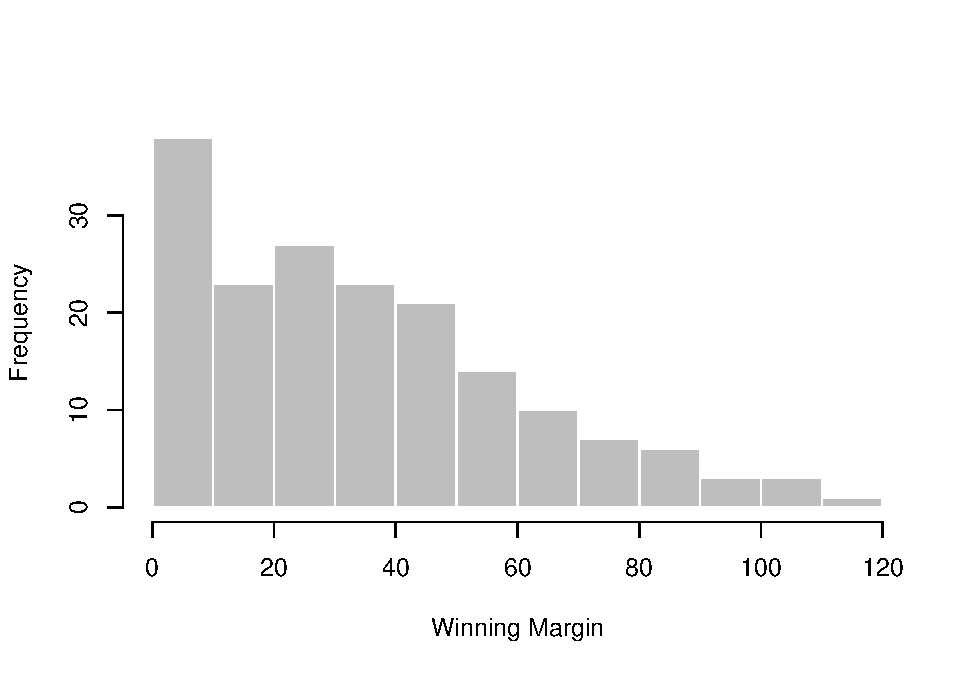
\includegraphics{schuster-statistics-remix_files/figure-latex/histogram1-1.pdf}
\caption{\label{fig:histogram1}A histogram of the AFL 2010 winning margin data (the \texttt{afl.margins} variable). As you might expect, the larger the margin the less frequently you tend to see it.}
\end{figure}

\hypertarget{centraltendency}{%
\section{Measures of central tendency}\label{centraltendency}}

Drawing pictures of the data, as I did in Figure \ref{fig:histogram1} is an excellent way to convey the ``gist'' of what the data is trying to tell you, it's often extremely useful to try to condense the data into a few simple ``summary'' statistics. In most situations, the first thing that you'll want to calculate is a measure of \textbf{\emph{central tendency}}. That is, you'd like to know something about the ``average'' or ``middle'' of your data lies. The two most commonly used measures are the mean, median and mode; occasionally people will also report a trimmed mean. I'll explain each of these in turn, and then discuss when each of them is useful.

\hypertarget{mean}{%
\subsection{The mean}\label{mean}}

The \textbf{\emph{mean}} of a set of observations is just a normal, old-fashioned average: add all of the values up, and then divide by the total number of values. The first five AFL margins were 56, 31, 56, 8 and 32, so the mean of these observations is just:
\[
\frac{56 + 31 + 56 + 8 + 32}{5} = \frac{183}{5} = 36.60
\]
Of course, this definition of the mean isn't news to anyone: averages (i.e., means) are used so often in everyday life that this is pretty familiar stuff. However, since the concept of a mean is something that everyone already understands, I'll use this as an excuse to start introducing some of the mathematical notation that statisticians use to describe this calculation, and talk about how the calculations would be done in R.

The first piece of notation to introduce is \(N\), which we'll use to refer to the number of observations that we're averaging (in this case \(N = 5\)). Next, we need to attach a label to the observations themselves. It's traditional to use \(X\) for this, and to use subscripts to indicate which observation we're actually talking about. That is, we'll use \(X_1\) to refer to the first observation, \(X_2\) to refer to the second observation, and so on, all the way up to \(X_N\) for the last one. Or, to say the same thing in a slightly more abstract way, we use \(X_i\) to refer to the \(i\)-th observation. Just to make sure we're clear on the notation, the following table lists the 5 observations in the \texttt{afl.margins} variable, along with the mathematical symbol used to refer to it, and the actual value that the observation corresponds to:

\begin{tabular}{lll}
\toprule
the observation & its symbol & the observed value\\
\midrule
winning margin, game 1 & \$X\_1\$ & 56 points\\
winning margin, game 2 & \$X\_2\$ & 31 points\\
winning margin, game 3 & \$X\_3\$ & 56 points\\
winning margin, game 4 & \$X\_4\$ & 8 points\\
winning margin, game 5 & \$X\_5\$ & 32 points\\
\bottomrule
\end{tabular}

Okay, now let's try to write a formula for the mean. By tradition, we use \(\bar{X}\) as the notation for the mean. So the calculation for the mean could be expressed using the following formula:
\[
\bar{X} = \frac{X_1 + X_2 + ... + X_{N-1} + X_N}{N}
\]
This formula is entirely correct, but it's terribly long, so we make use of the \textbf{\emph{summation symbol}} \(\scriptstyle\sum\) to shorten it.\footnote{The choice to use \(\Sigma\) to denote summation isn't arbitrary: it's the Greek upper case letter sigma, which is the analogue of the letter S in that alphabet. Similarly, there's an equivalent symbol used to denote the multiplication of lots of numbers: because multiplications are also called ``products'', we use the \(\Pi\) symbol for this; the Greek upper case pi, which is the analogue of the letter P.} If I want to add up the first five observations, I could write out the sum the long way, \(X_1 + X_2 + X_3 + X_4 +X_5\) or I could use the summation symbol to shorten it to this:
\[
\sum_{i=1}^5 X_i
\]
Taken literally, this could be read as ``the sum, taken over all \(i\) values from 1 to 5, of the value \(X_i\)''. But basically, what it means is ``add up the first five observations''. In any case, we can use this notation to write out the formula for the mean, which looks like this:
\[
\bar{X} = \frac{1}{N} \sum_{i=1}^N X_i 
\]

In all honesty, I can't imagine that all this mathematical notation helps clarify the concept of the mean at all. In fact, it's really just a fancy way of writing out the same thing I said in words: add all the values up, and then divide by the total number of items. However, that's not really the reason I went into all that detail. My goal was to try to make sure that everyone reading this book is clear on the notation that we'll be using throughout the book: \(\bar{X}\) for the mean, \(\scriptstyle\sum\) for the idea of summation, \(X_i\) for the \(i\)th observation, and \(N\) for the total number of observations. We're going to be re-using these symbols a fair bit, so it's important that you understand them well enough to be able to ``read'' the equations, and to be able to see that it's just saying ``add up lots of things and then divide by another thing''.

\hypertarget{calculating-the-mean-in-r}{%
\subsection{Calculating the mean in R}\label{calculating-the-mean-in-r}}

Okay that's the maths, how do we get the magic computing box to do the work for us? If you really wanted to, you could do this calculation directly in R. For the first 5 AFL scores, do this just by typing it in as if R were a calculator\ldots{}

\begin{Shaded}
\begin{Highlighting}[]
\NormalTok{(}\DecValTok{56} \SpecialCharTok{+} \DecValTok{31} \SpecialCharTok{+} \DecValTok{56} \SpecialCharTok{+} \DecValTok{8} \SpecialCharTok{+} \DecValTok{32}\NormalTok{) }\SpecialCharTok{/} \DecValTok{5}
\end{Highlighting}
\end{Shaded}

\begin{verbatim}
## [1] 36.6
\end{verbatim}

\ldots{} in which case R outputs the answer 36.6, just as if it were a calculator. However, that's not the only way to do the calculations, and when the number of observations starts to become large, it's easily the most tedious. Besides, in almost every real world scenario, you've already got the actual numbers stored in a variable of some kind, just like we have with the \texttt{afl.margins} variable. Under those circumstances, what you want is a function that will just add up all the values stored in a numeric vector. That's what the \texttt{sum()} function does. If we want to add up all 176 winning margins in the data set, we can do so using the following command:\footnote{Note that, just as we saw with the combine function \texttt{c()} and the remove function \texttt{rm()}, the \texttt{sum()} function has unnamed arguments. I'll talk about unnamed arguments later in Section \ref{dotsargument}, but for now let's just ignore this detail.}

\begin{Shaded}
\begin{Highlighting}[]
\FunctionTok{sum}\NormalTok{( afl.margins )}
\end{Highlighting}
\end{Shaded}

\begin{verbatim}
## [1] 6213
\end{verbatim}

If we only want the sum of the first five observations, then we can use square brackets to pull out only the first five elements of the vector. So the command would now be:

\begin{Shaded}
\begin{Highlighting}[]
\FunctionTok{sum}\NormalTok{( afl.margins[}\DecValTok{1}\SpecialCharTok{:}\DecValTok{5}\NormalTok{] )}
\end{Highlighting}
\end{Shaded}

\begin{verbatim}
## [1] 183
\end{verbatim}

To calculate the mean, we now tell R to divide the output of this summation by five, so the command that we need to type now becomes the following:

\begin{Shaded}
\begin{Highlighting}[]
\FunctionTok{sum}\NormalTok{( afl.margins[}\DecValTok{1}\SpecialCharTok{:}\DecValTok{5}\NormalTok{] ) }\SpecialCharTok{/} \DecValTok{5}
\end{Highlighting}
\end{Shaded}

\begin{verbatim}
## [1] 36.6
\end{verbatim}

Although it's pretty easy to calculate the mean using the \texttt{sum()} function, we can do it in an even easier way, since R also provides us with the \texttt{mean()} function. To calculate the mean for all 176 games, we would use the following command:

\begin{Shaded}
\begin{Highlighting}[]
\FunctionTok{mean}\NormalTok{( }\AttributeTok{x =}\NormalTok{ afl.margins )}
\end{Highlighting}
\end{Shaded}

\begin{verbatim}
## [1] 35.30114
\end{verbatim}

However, since \texttt{x} is the first argument to the function, I could have omitted the argument name. In any case, just to show you that there's nothing funny going on, here's what we would do to calculate the mean for the first five observations:

\begin{Shaded}
\begin{Highlighting}[]
\FunctionTok{mean}\NormalTok{( afl.margins[}\DecValTok{1}\SpecialCharTok{:}\DecValTok{5}\NormalTok{] )}
\end{Highlighting}
\end{Shaded}

\begin{verbatim}
## [1] 36.6
\end{verbatim}

As you can see, this gives exactly the same answers as the previous calculations.

\hypertarget{median}{%
\subsection{The median}\label{median}}

The second measure of central tendency that people use a lot is the \textbf{\emph{median}}, and it's even easier to describe than the mean. The median of a set of observations is just the middle value. As before let's imagine we were interested only in the first 5 AFL winning margins: 56, 31, 56, 8 and 32. To figure out the median, we sort these numbers into ascending order:
\[
8, 31, \mathbf{32}, 56, 56
\]
From inspection, it's obvious that the median value of these 5 observations is 32, since that's the middle one in the sorted list (I've put it in bold to make it even more obvious). Easy stuff. But what should we do if we were interested in the first 6 games rather than the first 5? Since the sixth game in the season had a winning margin of 14 points, our sorted list is now
\[
8, 14, \mathbf{31}, \mathbf{32}, 56, 56
\]
and there are \emph{two} middle numbers, 31 and 32. The median is defined as the average of those two numbers, which is of course 31.5. As before, it's very tedious to do this by hand when you've got lots of numbers. To illustrate this, here's what happens when you use R to sort all 176 winning margins. First, I'll use the \texttt{sort()} function (discussed in Chapter \ref{datahandling}) to display the winning margins in increasing numerical order:

\begin{Shaded}
\begin{Highlighting}[]
\FunctionTok{sort}\NormalTok{( }\AttributeTok{x =}\NormalTok{ afl.margins )}
\end{Highlighting}
\end{Shaded}

\begin{verbatim}
##   [1]   0   0   1   1   1   1   2   2   3   3   3   3   3   3   3   3   4
##  [18]   4   5   6   7   7   8   8   8   8   8   9   9   9   9   9   9  10
##  [35]  10  10  10  10  11  11  11  12  12  12  13  14  14  15  16  16  16
##  [52]  16  18  19  19  19  19  19  20  20  20  21  21  22  22  22  23  23
##  [69]  23  24  24  25  25  26  26  26  26  27  27  28  28  29  29  29  29
##  [86]  29  29  30  31  32  32  33  35  35  35  35  36  36  36  36  36  36
## [103]  37  38  38  38  38  38  39  39  40  41  42  43  43  44  44  44  44
## [120]  44  47  47  47  48  48  48  49  49  50  50  50  50  52  52  53  53
## [137]  54  54  55  55  55  56  56  56  57  60  61  61  63  64  65  65  66
## [154]  67  68  70  71  71  72  73  75  75  76  81  82  82  83  84  89  94
## [171]  95  98 101 104 108 116
\end{verbatim}

The middle values are 30 and 31, so the median winning margin for 2010 was 30.5 points. In real life, of course, no-one actually calculates the median by sorting the data and then looking for the middle value. In real life, we use the median command:

\begin{Shaded}
\begin{Highlighting}[]
\FunctionTok{median}\NormalTok{( }\AttributeTok{x =}\NormalTok{ afl.margins )}
\end{Highlighting}
\end{Shaded}

\begin{verbatim}
## [1] 30.5
\end{verbatim}

which outputs the median value of 30.5.

\hypertarget{mean-or-median-whats-the-difference}{%
\subsection{Mean or median? What's the difference?}\label{mean-or-median-whats-the-difference}}

\begin{figure}
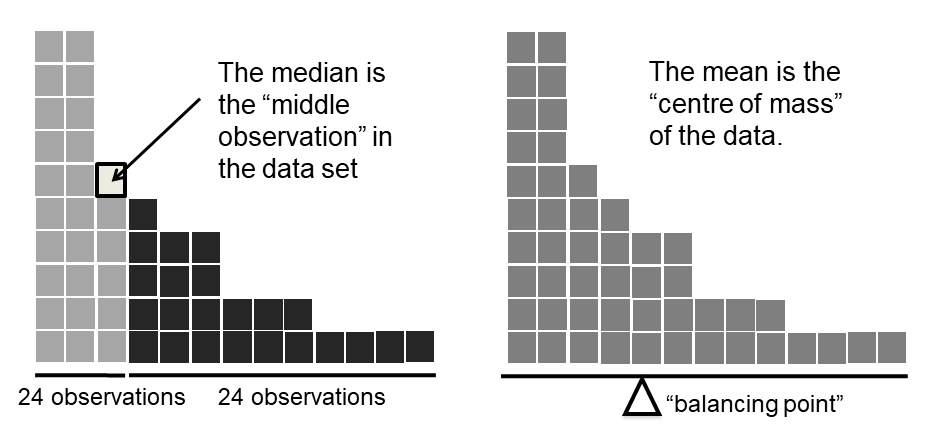
\includegraphics[width=12.86in]{./img/descriptives2/meanmedian} \caption{An illustration of the difference between how the mean and the median should be interpreted. The mean is basically the "centre of gravity" of the data set: if you imagine that the histogram of the data is a solid object, then the point on which you could balance it (as if on a see-saw) is the mean. In contrast, the median is the middle observation. Half of the observations are smaller, and half of the observations are larger.}\label{fig:meanmedian}
\end{figure}

Knowing how to calculate means and medians is only a part of the story. You also need to understand what each one is saying about the data, and what that implies for when you should use each one. This is illustrated in Figure \ref{fig:meanmedian} the mean is kind of like the ``centre of gravity'' of the data set, whereas the median is the ``middle value'' in the data. What this implies, as far as which one you should use, depends a little on what type of data you've got and what you're trying to achieve. As a rough guide:

\begin{itemize}
\tightlist
\item
  If your data are nominal scale, you probably shouldn't be using either the mean or the median. Both the mean and the median rely on the idea that the numbers assigned to values are meaningful. If the numbering scheme is arbitrary, then it's probably best to use the mode (Section \ref{mode}) instead.
\item
  If your data are ordinal scale, you're more likely to want to use the median than the mean. The median only makes use of the order information in your data (i.e., which numbers are bigger), but doesn't depend on the precise numbers involved. That's exactly the situation that applies when your data are ordinal scale. The mean, on the other hand, makes use of the precise numeric values assigned to the observations, so it's not really appropriate for ordinal data.
\item
  For interval and ratio scale data, either one is generally acceptable. Which one you pick depends a bit on what you're trying to achieve. The mean has the advantage that it uses all the information in the data (which is useful when you don't have a lot of data), but it's very sensitive to extreme values, as we'll see in Section \ref{trimmedmean}.
\end{itemize}

Let's expand on that last part a little. One consequence is that there's systematic differences between the mean and the median when the histogram is asymmetric (skewed; see Section \ref{skewandkurtosis}). This is illustrated in Figure \ref{fig:meanmedian} notice that the median (right hand side) is located closer to the ``body'' of the histogram, whereas the mean (left hand side) gets dragged towards the ``tail'' (where the extreme values are). To give a concrete example, suppose Bob (income \$50,000), Kate (income \$60,000) and Jane (income \$65,000) are sitting at a table: the average income at the table is \$58,333 and the median income is \$60,000. Then Bill sits down with them (income \$100,000,000). The average income has now jumped to \$25,043,750 but the median rises only to \$62,500. If you're interested in looking at the overall income at the table, the mean might be the right answer; but if you're interested in what counts as a typical income at the table, the median would be a better choice here.

\hypertarget{housingpriceexample}{%
\subsection{A real life example}\label{housingpriceexample}}

To try to get a sense of why you need to pay attention to the differences between the mean and the median, let's consider a real life example. Since I tend to mock journalists for their poor scientific and statistical knowledge, I should give credit where credit is due. This is from an excellent article on the ABC news website\footnote{www.abc.net.au/news/stories/2010/09/24/3021480.htm} 24 September, 2010:

\begin{quote}
Senior Commonwealth Bank executives have travelled the world in the past couple of weeks with a presentation showing how Australian house prices, and the key price to income ratios, compare favourably with similar countries. ``Housing affordability has actually been going sideways for the last five to six years,'' said Craig James, the chief economist of the bank's trading arm, CommSec.
\end{quote}

This probably comes as a huge surprise to anyone with a mortgage, or who wants a mortgage, or pays rent, or isn't completely oblivious to what's been going on in the Australian housing market over the last several years. Back to the article:

\begin{quote}
CBA has waged its war against what it believes are housing doomsayers with graphs, numbers and international comparisons. In its presentation, the bank rejects arguments that Australia's housing is relatively expensive compared to incomes. It says Australia's house price to household income ratio of 5.6 in the major cities, and 4.3 nationwide, is comparable to many other developed nations. It says San Francisco and New York have ratios of 7, Auckland's is 6.7, and Vancouver comes in at 9.3.
\end{quote}

More excellent news! Except, the article goes on to make the observation that\ldots{}

\begin{quote}
Many analysts say that has led the bank to use misleading figures and comparisons. If you go to page four of CBA's presentation and read the source information at the bottom of the graph and table, you would notice there is an additional source on the international comparison -- Demographia. However, if the Commonwealth Bank had also used Demographia's analysis of Australia's house price to income ratio, it would have come up with a figure closer to 9 rather than 5.6 or 4.3
\end{quote}

That's, um, a rather serious discrepancy. One group of people say 9, another says 4-5. Should we just split the difference, and say the truth lies somewhere in between? Absolutely not: this is a situation where there is a right answer and a wrong answer. Demographia are correct, and the Commonwealth Bank is incorrect. As the article points out

\begin{quote}
{[}An{]} obvious problem with the Commonwealth Bank's domestic price to income figures is they compare average incomes with median house prices (unlike the Demographia figures that compare median incomes to median prices). The median is the mid-point, effectively cutting out the highs and lows, and that means the average is generally higher when it comes to incomes and asset prices, because it includes the earnings of Australia's wealthiest people. To put it another way: the Commonwealth Bank's figures count Ralph Norris' multi-million dollar pay packet on the income side, but not his (no doubt) very expensive house in the property price figures, thus understating the house price to income ratio for middle-income Australians.
\end{quote}

Couldn't have put it better myself. The way that Demographia calculated the ratio is the right thing to do. The way that the Bank did it is incorrect. As for why an extremely quantitatively sophisticated organisation such as a major bank made such an elementary mistake, well\ldots{} I can't say for sure, since I have no special insight into their thinking, but the article itself does happen to mention the following facts, which may or may not be relevant:

\begin{quote}
{[}As{]} Australia's largest home lender, the Commonwealth Bank has one of the biggest vested interests in house prices rising. It effectively owns a massive swathe of Australian housing as security for its home loans as well as many small business loans.
\end{quote}

My, my.

\hypertarget{trimmedmean}{%
\subsection{Trimmed mean}\label{trimmedmean}}

One of the fundamental rules of applied statistics is that the data are messy. Real life is never simple, and so the data sets that you obtain are never as straightforward as the statistical theory says.\footnote{Or at least, the basic statistical theory -- these days there is a whole subfield of statistics called \emph{robust statistics} that tries to grapple with the messiness of real data and develop theory that can cope with it.} This can have awkward consequences. To illustrate, consider this rather strange looking data set:
\[
-100,2,3,4,5,6,7,8,9,10
\]
If you were to observe this in a real life data set, you'd probably suspect that something funny was going on with the \(-100\) value. It's probably an \textbf{\emph{outlier}}, a value that doesn't really belong with the others. You might consider removing it from the data set entirely, and in this particular case I'd probably agree with that course of action. In real life, however, you don't always get such cut-and-dried examples. For instance, you might get this instead:
\[
-15,2,3,4,5,6,7,8,9,12
\]
The \(-15\) looks a bit suspicious, but not anywhere near as much as that \(-100\) did. In this case, it's a little trickier. It \emph{might} be a legitimate observation, it might not.

When faced with a situation where some of the most extreme-valued observations might not be quite trustworthy, the mean is not necessarily a good measure of central tendency. It is highly sensitive to one or two extreme values, and is thus not considered to be a \textbf{\emph{robust}} measure. One remedy that we've seen is to use the median. A more general solution is to use a ``trimmed mean''. To calculate a trimmed mean, what you do is ``discard'' the most extreme examples on both ends (i.e., the largest and the smallest), and then take the mean of everything else. The goal is to preserve the best characteristics of the mean and the median: just like a median, you aren't highly influenced by extreme outliers, but like the mean, you ``use'' more than one of the observations. Generally, we describe a trimmed mean in terms of the percentage of observation on either side that are discarded. So, for instance, a 10\% trimmed mean discards the largest 10\% of the observations \emph{and} the smallest 10\% of the observations, and then takes the mean of the remaining 80\% of the observations. Not surprisingly, the 0\% trimmed mean is just the regular mean, and the 50\% trimmed mean is the median. In that sense, trimmed means provide a whole family of central tendency measures that span the range from the mean to the median.

For our toy example above, we have 10 observations, and so a 10\% trimmed mean is calculated by ignoring the largest value (i.e., \texttt{12}) and the smallest value (i.e., \texttt{-15}) and taking the mean of the remaining values. First, let's enter the data

\begin{Shaded}
\begin{Highlighting}[]
\NormalTok{dataset }\OtherTok{\textless{}{-}} \FunctionTok{c}\NormalTok{( }\SpecialCharTok{{-}}\DecValTok{15}\NormalTok{,}\DecValTok{2}\NormalTok{,}\DecValTok{3}\NormalTok{,}\DecValTok{4}\NormalTok{,}\DecValTok{5}\NormalTok{,}\DecValTok{6}\NormalTok{,}\DecValTok{7}\NormalTok{,}\DecValTok{8}\NormalTok{,}\DecValTok{9}\NormalTok{,}\DecValTok{12}\NormalTok{ )}
\end{Highlighting}
\end{Shaded}

Next, let's calculate means and medians:

\begin{Shaded}
\begin{Highlighting}[]
\FunctionTok{mean}\NormalTok{( }\AttributeTok{x =}\NormalTok{ dataset )}
\end{Highlighting}
\end{Shaded}

\begin{verbatim}
## [1] 4.1
\end{verbatim}

\begin{Shaded}
\begin{Highlighting}[]
\FunctionTok{median}\NormalTok{( }\AttributeTok{x =}\NormalTok{ dataset )}
\end{Highlighting}
\end{Shaded}

\begin{verbatim}
## [1] 5.5
\end{verbatim}

That's a fairly substantial difference, but I'm tempted to think that the mean is being influenced a bit too much by the extreme values at either end of the data set, especially the \(-15\) one. So let's just try trimming the mean a bit. If I take a 10\% trimmed mean, we'll drop the extreme values on either side, and take the mean of the rest:

\begin{Shaded}
\begin{Highlighting}[]
\FunctionTok{mean}\NormalTok{( }\AttributeTok{x =}\NormalTok{ dataset, }\AttributeTok{trim =}\NormalTok{ .}\DecValTok{1}\NormalTok{)}
\end{Highlighting}
\end{Shaded}

\begin{verbatim}
## [1] 5.5
\end{verbatim}

which in this case gives exactly the same answer as the median. Note that, to get a 10\% trimmed mean you write \texttt{trim\ =\ .1}, not \texttt{trim\ =\ 10}. In any case, let's finish up by calculating the 5\% trimmed mean for the \texttt{afl.margins} data,

\begin{Shaded}
\begin{Highlighting}[]
\FunctionTok{mean}\NormalTok{( }\AttributeTok{x =}\NormalTok{ afl.margins, }\AttributeTok{trim =}\NormalTok{ .}\DecValTok{05}\NormalTok{)  }
\end{Highlighting}
\end{Shaded}

\begin{verbatim}
## [1] 33.75
\end{verbatim}

\hypertarget{mode}{%
\subsection{Mode}\label{mode}}

The mode of a sample is very simple: it is the value that occurs most frequently. To illustrate the mode using the AFL data, let's examine a different aspect to the data set. Who has played in the most finals? The \texttt{afl.finalists} variable is a factor that contains the name of every team that played in any AFL final from 1987-2010, so let's have a look at it. To do this we will use the \texttt{head()} command. \texttt{head()} is useful when you're working with a data.frame with a lot of rows since you can use it to tell you how many rows to return. There have been a lot of finals in this period so printing afl.finalists using \texttt{print(afl.finalists)} will just fill us the screen. The command below tells R we just want the first 25 rows of the data.frame.

\begin{Shaded}
\begin{Highlighting}[]
\FunctionTok{head}\NormalTok{(afl.finalists, }\DecValTok{25}\NormalTok{)}
\end{Highlighting}
\end{Shaded}

\begin{verbatim}
##  [1] Hawthorn    Melbourne   Carlton     Melbourne   Hawthorn   
##  [6] Carlton     Melbourne   Carlton     Hawthorn    Melbourne  
## [11] Melbourne   Hawthorn    Melbourne   Essendon    Hawthorn   
## [16] Geelong     Geelong     Hawthorn    Collingwood Melbourne  
## [21] Collingwood West Coast  Collingwood Essendon    Collingwood
## 17 Levels: Adelaide Brisbane Carlton Collingwood Essendon ... Western Bulldogs
\end{verbatim}

There are actually 400 entries (aren't you glad we didn't print them all?). We \emph{could} read through all 400, and count the number of occasions on which each team name appears in our list of finalists, thereby producing a \textbf{\emph{frequency table}}. However, that would be mindless and boring: exactly the sort of task that computers are great at. So let's use the \texttt{table()} function (discussed in more detail in Section \ref{freqtables}) to do this task for us:

\begin{Shaded}
\begin{Highlighting}[]
\FunctionTok{table}\NormalTok{( afl.finalists )}
\end{Highlighting}
\end{Shaded}

\begin{verbatim}
## afl.finalists
##         Adelaide         Brisbane          Carlton      Collingwood 
##               26               25               26               28 
##         Essendon          Fitzroy        Fremantle          Geelong 
##               32                0                6               39 
##         Hawthorn        Melbourne  North Melbourne    Port Adelaide 
##               27               28               28               17 
##         Richmond         St Kilda           Sydney       West Coast 
##                6               24               26               38 
## Western Bulldogs 
##               24
\end{verbatim}

Now that we have our frequency table, we can just look at it and see that, over the 24 years for which we have data, Geelong has played in more finals than any other team. Thus, the mode of the \texttt{finalists} data is \texttt{"Geelong"}. The core packages in R don't have a function for calculating the mode\footnote{As we saw earlier, it \emph{does} have a function called \texttt{mode()}, but it does something completely different.}. However, I've included a function in the \texttt{lsr} package that does this. The function is called \texttt{modeOf()}, and here's how you use it:

\begin{Shaded}
\begin{Highlighting}[]
\FunctionTok{modeOf}\NormalTok{( }\AttributeTok{x =}\NormalTok{ afl.finalists )}
\end{Highlighting}
\end{Shaded}

\begin{verbatim}
## [1] "Geelong"
\end{verbatim}

There's also a function called \texttt{maxFreq()} that tells you what the modal frequency is. If we apply this function to our finalists data, we obtain the following:

\begin{Shaded}
\begin{Highlighting}[]
\FunctionTok{maxFreq}\NormalTok{( }\AttributeTok{x =}\NormalTok{ afl.finalists )}
\end{Highlighting}
\end{Shaded}

\begin{verbatim}
## [1] 39
\end{verbatim}

Taken together, we observe that Geelong (39 finals) played in more finals than any other team during the 1987-2010 period.

One last point to make with respect to the mode. While it's generally true that the mode is most often calculated when you have nominal scale data (because means and medians are useless for those sorts of variables), there are some situations in which you really do want to know the mode of an ordinal, interval or ratio scale variable. For instance, let's go back to thinking about our \texttt{afl.margins} variable. This variable is clearly ratio scale (if it's not clear to you, it may help to re-read Section \ref{scales}), and so in most situations the mean or the median is the measure of central tendency that you want. But consider this scenario\ldots{} a friend of yours is offering a bet. They pick a football game at random, and (without knowing who is playing) you have to guess the \emph{exact} margin. If you guess correctly, you win \$50. If you don't, you lose \$1. There are no consolation prizes for ``almost'' getting the right answer. You have to guess exactly the right margin\footnote{This is called a ``0-1 loss function'', meaning that you either win (1) or you lose (0), with no middle ground.} For this bet, the mean and the median are completely useless to you. It is the mode that you should bet on. So, we calculate this modal value

\begin{Shaded}
\begin{Highlighting}[]
\FunctionTok{modeOf}\NormalTok{( }\AttributeTok{x =}\NormalTok{ afl.margins )}
\end{Highlighting}
\end{Shaded}

\begin{verbatim}
## [1] 3
\end{verbatim}

\begin{Shaded}
\begin{Highlighting}[]
\FunctionTok{maxFreq}\NormalTok{( }\AttributeTok{x =}\NormalTok{ afl.margins )}
\end{Highlighting}
\end{Shaded}

\begin{verbatim}
## [1] 8
\end{verbatim}

So the 2010 data suggest you should bet on a 3 point margin, and since this was observed in 8 of the 176 game (4.5\% of games) the odds are firmly in your favour.

\hypertarget{var}{%
\section{Measures of variability}\label{var}}

The statistics that we've discussed so far all relate to \emph{central tendency}. That is, they all talk about which values are ``in the middle'' or ``popular'' in the data. However, central tendency is not the only type of summary statistic that we want to calculate. The second thing that we really want is a measure of the \textbf{\emph{variability}} of the data. That is, how ``spread out'' are the data? How ``far'' away from the mean or median do the observed values tend to be? For now, let's assume that the data are interval or ratio scale, so we'll continue to use the \texttt{afl.margins} data. We'll use this data to discuss several different measures of spread, each with different strengths and weaknesses.

\hypertarget{range}{%
\subsection{Range}\label{range}}

The \textbf{\emph{range}} of a variable is very simple: it's the biggest value minus the smallest value. For the AFL winning margins data, the maximum value is 116, and the minimum value is 0. We can calculate these values in R using the \texttt{max()} and \texttt{min()} functions:

\begin{Shaded}
\begin{Highlighting}[]
\FunctionTok{max}\NormalTok{( afl.margins )}
\end{Highlighting}
\end{Shaded}

\begin{verbatim}
## [1] 116
\end{verbatim}

\begin{Shaded}
\begin{Highlighting}[]
\FunctionTok{min}\NormalTok{( afl.margins )}
\end{Highlighting}
\end{Shaded}

\begin{verbatim}
## [1] 0
\end{verbatim}

where I've omitted the output because it's not interesting. The other possibility is to use the \texttt{range()} function; which outputs both the minimum value and the maximum value in a vector, like this:

\begin{Shaded}
\begin{Highlighting}[]
\FunctionTok{range}\NormalTok{( afl.margins )}
\end{Highlighting}
\end{Shaded}

\begin{verbatim}
## [1]   0 116
\end{verbatim}

Although the range is the simplest way to quantify the notion of ``variability'', it's one of the worst. Recall from our discussion of the mean that we want our summary measure to be robust. If the data set has one or two extremely bad values in it, we'd like our statistics not to be unduly influenced by these cases. If we look once again at our toy example of a data set containing very extreme outliers\ldots{}
\[
-100,2,3,4,5,6,7,8,9,10
\]
\ldots{} it is clear that the range is not robust, since this has a range of 110, but if the outlier were removed we would have a range of only 8.

\hypertarget{interquartile-range}{%
\subsection{Interquartile range}\label{interquartile-range}}

The \textbf{\emph{interquartile range}} (IQR) is like the range, but instead of calculating the difference between the biggest and smallest value, it calculates the difference between the 25th quantile and the 75th quantile. Probably you already know what a \textbf{\emph{quantile}} is (they're more commonly called percentiles), but if not: the 10th percentile of a data set is the smallest number \(x\) such that 10\% of the data is less than \(x\). In fact, we've already come across the idea: the median of a data set is its 50th quantile / percentile! R actually provides you with a way of calculating quantiles, using the (surprise, surprise) \texttt{quantile()} function. Let's use it to calculate the median AFL winning margin:

\begin{Shaded}
\begin{Highlighting}[]
\FunctionTok{quantile}\NormalTok{( }\AttributeTok{x =}\NormalTok{ afl.margins, }\AttributeTok{probs =}\NormalTok{ .}\DecValTok{5}\NormalTok{)}
\end{Highlighting}
\end{Shaded}

\begin{verbatim}
##  50% 
## 30.5
\end{verbatim}

And not surprisingly, this agrees with the answer that we saw earlier with the \texttt{median()} function. Now, we can actually input lots of quantiles at once, by specifying a vector for the \texttt{probs} argument. So lets do that, and get the 25th and 75th percentile:

\begin{Shaded}
\begin{Highlighting}[]
\FunctionTok{quantile}\NormalTok{( }\AttributeTok{x =}\NormalTok{ afl.margins, }\AttributeTok{probs =} \FunctionTok{c}\NormalTok{(.}\DecValTok{25}\NormalTok{,.}\DecValTok{75}\NormalTok{) )}
\end{Highlighting}
\end{Shaded}

\begin{verbatim}
##   25%   75% 
## 12.75 50.50
\end{verbatim}

And, by noting that \(50.5 - 12.75 = 37.75\), we can see that the interquartile range for the 2010 AFL winning margins data is 37.75. Of course, that seems like too much work to do all that typing, so R has a built in function called \texttt{IQR()} that we can use:

\begin{Shaded}
\begin{Highlighting}[]
\FunctionTok{IQR}\NormalTok{( }\AttributeTok{x =}\NormalTok{ afl.margins )}
\end{Highlighting}
\end{Shaded}

\begin{verbatim}
## [1] 37.75
\end{verbatim}

While it's obvious how to interpret the range, it's a little less obvious how to interpret the IQR. The simplest way to think about it is like this: the interquartile range is the range spanned by the ``middle half'' of the data. That is, one quarter of the data falls below the 25th percentile, one quarter of the data is above the 75th percentile, leaving the ``middle half'' of the data lying in between the two. And the IQR is the range covered by that middle half.

\hypertarget{aad}{%
\subsection{Mean absolute deviation}\label{aad}}

The two measures we've looked at so far, the range and the interquartile range, both rely on the idea that we can measure the spread of the data by looking at the quantiles of the data. However, this isn't the only way to think about the problem. A different approach is to select a meaningful reference point (usually the mean or the median) and then report the ``typical'' deviations from that reference point. What do we mean by ``typical'' deviation? Usually, the mean or median value of these deviations! In practice, this leads to two different measures, the ``mean absolute deviation (from the mean)'' and the ``median absolute deviation (from the median)''. From what I've read, the measure based on the median seems to be used in statistics, and does seem to be the better of the two, but to be honest I don't think I've seen it used much in psychology. The measure based on the mean does occasionally show up in psychology though. In this section I'll talk about the first one, and I'll come back to talk about the second one later.

Since the previous paragraph might sound a little abstract, let's go through the \textbf{\emph{mean absolute deviation}} from the mean a little more slowly. One useful thing about this measure is that the name actually tells you exactly how to calculate it. Let's think about our AFL winning margins data, and once again we'll start by pretending that there's only 5 games in total, with winning margins of 56, 31, 56, 8 and 32. Since our calculations rely on an examination of the deviation from some reference point (in this case the mean), the first thing we need to calculate is the mean, \(\bar{X}\). For these five observations, our mean is \(\bar{X} = 36.6\). The next step is to convert each of our observations \(X_i\) into a deviation score. We do this by calculating the difference between the observation \(X_i\) and the mean \(\bar{X}\). That is, the deviation score is defined to be \(X_i - \bar{X}\). For the first observation in our sample, this is equal to \(56 - 36.6 = 19.4\). Okay, that's simple enough. The next step in the process is to convert these deviations to absolute deviations. As we discussed earlier when talking about the \texttt{abs()} function in R (Section \ref{usingfunctions}), we do this by converting any negative values to positive ones. Mathematically, we would denote the absolute value of \(-3\) as \(|-3|\), and so we say that \(|-3| = 3\). We use the absolute value function here because we don't really care whether the value is higher than the mean or lower than the mean, we're just interested in how \emph{close} it is to the mean. To help make this process as obvious as possible, the table below shows these calculations for all five observations:

\begin{tabular}{lll}
\toprule
the observation & its symbol & the observed value\\
\midrule
winning margin, game 1 & \$X\_1\$ & 56 points\\
winning margin, game 2 & \$X\_2\$ & 31 points\\
winning margin, game 3 & \$X\_3\$ & 56 points\\
winning margin, game 4 & \$X\_4\$ & 8 points\\
winning margin, game 5 & \$X\_5\$ & 32 points\\
\bottomrule
\end{tabular}

Now that we have calculated the absolute deviation score for every observation in the data set, all that we have to do to calculate the mean of these scores. Let's do that:
\[
\frac{19.4 + 5.6 + 19.4 + 28.6 + 4.6}{5} = 15.52
\]
And we're done. The mean absolute deviation for these five scores is 15.52.

However, while our calculations for this little example are at an end, we do have a couple of things left to talk about. Firstly, we should really try to write down a proper mathematical formula. But in order do to this I need some mathematical notation to refer to the mean absolute deviation. Irritatingly, ``mean absolute deviation'' and ``median absolute deviation'' have the same acronym (MAD), which leads to a certain amount of ambiguity, and since R tends to use MAD to refer to the median absolute deviation, I'd better come up with something different for the mean absolute deviation. Sigh. What I'll do is use AAD instead, short for \emph{average} absolute deviation. Now that we have some unambiguous notation, here's the formula that describes what we just calculated:
\[
\mbox{}(X) = \frac{1}{N} \sum_{i = 1}^N |X_i - \bar{X}|
\]

The last thing we need to talk about is how to calculate AAD in R. One possibility would be to do everything using low level commands, laboriously following the same steps that I used when describing the calculations above. However, that's pretty tedious. You'd end up with a series of commands that might look like this:

\begin{Shaded}
\begin{Highlighting}[]
\NormalTok{X }\OtherTok{\textless{}{-}} \FunctionTok{c}\NormalTok{(}\DecValTok{56}\NormalTok{, }\DecValTok{31}\NormalTok{,}\DecValTok{56}\NormalTok{,}\DecValTok{8}\NormalTok{,}\DecValTok{32}\NormalTok{)   }\CommentTok{\# enter the data}
\NormalTok{X.bar }\OtherTok{\textless{}{-}} \FunctionTok{mean}\NormalTok{( X )       }\CommentTok{\# step 1. the mean of the data}
\NormalTok{AD }\OtherTok{\textless{}{-}} \FunctionTok{abs}\NormalTok{( X }\SpecialCharTok{{-}}\NormalTok{ X.bar )   }\CommentTok{\# step 2. the absolute deviations from the mean}
\NormalTok{AAD }\OtherTok{\textless{}{-}} \FunctionTok{mean}\NormalTok{( AD )        }\CommentTok{\# step 3. the mean absolute deviations}
\FunctionTok{print}\NormalTok{( AAD )             }\CommentTok{\# print the results}
\end{Highlighting}
\end{Shaded}

\begin{verbatim}
## [1] 15.52
\end{verbatim}

Each of those commands is pretty simple, but there's just too many of them. And because I find that to be too much typing, the \texttt{lsr} package has a very simple function called \texttt{aad()} that does the calculations for you. If we apply the \texttt{aad()} function to our data, we get this:

\begin{Shaded}
\begin{Highlighting}[]
\FunctionTok{library}\NormalTok{(lsr)}
\FunctionTok{aad}\NormalTok{( X )}
\end{Highlighting}
\end{Shaded}

\begin{verbatim}
## [1] 15.52
\end{verbatim}

No suprises there.

\hypertarget{variance}{%
\subsection{Variance}\label{variance}}

Although the mean absolute deviation measure has its uses, it's not the best measure of variability to use. From a purely mathematical perspective, there are some solid reasons to prefer squared deviations rather than absolute deviations. If we do that, we obtain a measure is called the \textbf{\emph{variance}}, which has a lot of really nice statistical properties that I'm going to ignore,\footnote{Well, I will very briefly mention the one that I think is coolest, for a very particular definition of ``cool'', that is. Variances are \emph{additive}. Here's what that means: suppose I have two variables \(X\) and \(Y\), whose variances are \$\mbox{Var}}(X)\$ and \(\mbox{Var}(Y)\) respectively. Now imagine I want to define a new variable \(Z\) that is the sum of the two, \(Z = X+Y\). As it turns out, the variance of \(Z\) is equal to \(\mbox{Var}(X) + \mbox{Var}(Y)\). This is a \emph{very} useful property, but it's not true of the other measures that I talk about in this section.{]} and one massive psychological flaw that I'm going to make a big deal out of in a moment. The variance of a data set \(X\) is sometimes written as \(\mbox{Var}(X)\), but it's more commonly denoted \(s^2\) (the reason for this will become clearer shortly). The formula that we use to calculate the variance of a set of observations is as follows:
\[
\mbox{Var}(X) = \frac{1}{N} \sum_{i=1}^N \left( X_i - \bar{X} \right)^2
\]
\[\mbox{Var}(X) = \frac{\sum_{i=1}^N \left( X_i - \bar{X} \right)^2}{N}\]
As you can see, it's basically the same formula that we used to calculate the mean absolute deviation, except that instead of using ``absolute deviations'' we use ``squared deviations''. It is for this reason that the variance is sometimes referred to as the ``mean square deviation''.

Now that we've got the basic idea, let's have a look at a concrete example. Once again, let's use the first five AFL games as our data. If we follow the same approach that we took last time, we end up with the following table:

\begin{table}

\caption{\label{tab:unnamed-chunk-194}Basic arithmetic operations in R. These five operators are used very frequently throughout the text, so it's important to be familiar with them at the outset.}
\centering
\begin{tabular}[t]{lllll}
\toprule
Notation [English] & \$i\$ [which game] & \$X\_i\$ [value] & \$X\_i - \textbackslash{}bar\{X\}\$ [deviation from mean] & \$(X\_i - \textbackslash{}bar\{X\})\textasciicircum{}2\$ [absolute deviation]\\
\midrule
 & 1 & 56 & 19.4 & 376.36\\
 & 2 & 31 & -5.6 & 31.36\\
 & 3 & 56 & 19.4 & 376.36\\
 & 4 & 8 & -28.6 & 817.96\\
 & 5 & 32 & -4.6 & 21.16\\
\bottomrule
\end{tabular}
\end{table}

That last column contains all of our squared deviations, so all we have to do is average them. If we do that by typing all the numbers into R by hand\ldots{}

\begin{Shaded}
\begin{Highlighting}[]
\NormalTok{( }\FloatTok{376.36} \SpecialCharTok{+} \FloatTok{31.36} \SpecialCharTok{+} \FloatTok{376.36} \SpecialCharTok{+} \FloatTok{817.96} \SpecialCharTok{+} \FloatTok{21.16}\NormalTok{ ) }\SpecialCharTok{/} \DecValTok{5}
\end{Highlighting}
\end{Shaded}

\begin{verbatim}
## [1] 324.64
\end{verbatim}

\ldots{} we end up with a variance of 324.64. Exciting, isn't it? For the moment, let's ignore the burning question that you're all probably thinking (i.e., what the heck does a variance of 324.64 actually mean?) and instead talk a bit more about how to do the calculations in R, because this will reveal something very weird.

As always, we want to avoid having to type in a whole lot of numbers ourselves. And as it happens, we have the vector \texttt{X} lying around, which we created in the previous section. With this in mind, we can calculate the variance of \texttt{X} by using the following command,

\begin{Shaded}
\begin{Highlighting}[]
\FunctionTok{mean}\NormalTok{( (X }\SpecialCharTok{{-}} \FunctionTok{mean}\NormalTok{(X) )}\SpecialCharTok{\^{}}\DecValTok{2}\NormalTok{)}
\end{Highlighting}
\end{Shaded}

\begin{verbatim}
## [1] 324.64
\end{verbatim}

and as usual we get the same answer as the one that we got when we did everything by hand. However, I \emph{still} think that this is too much typing. Fortunately, R has a built in function called \texttt{var()} which does calculate variances. So we could also do this\ldots{}

\begin{Shaded}
\begin{Highlighting}[]
\FunctionTok{var}\NormalTok{(X)}
\end{Highlighting}
\end{Shaded}

\begin{verbatim}
## [1] 405.8
\end{verbatim}

and you get the same\ldots{} no, wait\ldots{} you get a completely \emph{different} answer. That's just weird. Is R broken? Is this a typo? Is Dan an idiot?

As it happens, the answer is no.\footnote{With the possible exception of the third question.} It's not a typo, and R is not making a mistake. To get a feel for what's happening, let's stop using the tiny data set containing only 5 data points, and switch to the full set of 176 games that we've got stored in our \texttt{afl.margins} vector. First, let's calculate the variance by using the formula that I described above:

\begin{Shaded}
\begin{Highlighting}[]
\FunctionTok{mean}\NormalTok{( (afl.margins }\SpecialCharTok{{-}} \FunctionTok{mean}\NormalTok{(afl.margins) )}\SpecialCharTok{\^{}}\DecValTok{2}\NormalTok{)}
\end{Highlighting}
\end{Shaded}

\begin{verbatim}
## [1] 675.9718
\end{verbatim}

Now let's use the \texttt{var()} function:

\begin{Shaded}
\begin{Highlighting}[]
\FunctionTok{var}\NormalTok{( afl.margins )}
\end{Highlighting}
\end{Shaded}

\begin{verbatim}
## [1] 679.8345
\end{verbatim}

Hm. These two numbers are very similar this time. That seems like too much of a coincidence to be a mistake. And of course it isn't a mistake. In fact, it's very simple to explain what R is doing here, but slightly trickier to explain \emph{why} R is doing it. So let's start with the ``what''. What R is doing is evaluating a slightly different formula to the one I showed you above. Instead of averaging the squared deviations, which requires you to divide by the number of data points \(N\), R has chosen to divide by \(N-1\). In other words, the formula that R is using is this one\\
\[
\frac{1}{N-1} \sum_{i=1}^N \left( X_i - \bar{X} \right)^2
\]
It's easy enough to verify that this is what's happening, as the following command illustrates:

\begin{Shaded}
\begin{Highlighting}[]
\FunctionTok{sum}\NormalTok{( (X}\SpecialCharTok{{-}}\FunctionTok{mean}\NormalTok{(X))}\SpecialCharTok{\^{}}\DecValTok{2}\NormalTok{ ) }\SpecialCharTok{/} \DecValTok{4}
\end{Highlighting}
\end{Shaded}

\begin{verbatim}
## [1] 405.8
\end{verbatim}

This is the same answer that R gave us originally when we calculated \texttt{var(X)} originally. So that's the \emph{what}. The real question is \emph{why} R is dividing by \(N-1\) and not by \(N\). After all, the variance is supposed to be the \emph{mean} squared deviation, right? So shouldn't we be dividing by \(N\), the actual number of observations in the sample? Well, yes, we should. However, as we'll discuss in Chapter \ref{estimation}, there's a subtle distinction between ``describing a sample'' and ``making guesses about the population from which the sample came''. Up to this point, it's been a distinction without a difference. Regardless of whether you're describing a sample or drawing inferences about the population, the mean is calculated exactly the same way. Not so for the variance, or the standard deviation, or for many other measures besides. What I outlined to you initially (i.e., take the actual average, and thus divide by \(N\)) assumes that you literally intend to calculate the variance of the sample. Most of the time, however, you're not terribly interested in the sample \emph{in and of itself}. Rather, the sample exists to tell you something about the world. If so, you're actually starting to move away from calculating a ``sample statistic'', and towards the idea of estimating a ``population parameter''. However, I'm getting ahead of myself. For now, let's just take it on faith that R knows what it's doing, and we'll revisit the question later on when we talk about estimation in Chapter \ref{estimation}.

Okay, one last thing. This section so far has read a bit like a mystery novel. I've shown you how to calculate the variance, described the weird ``\(N-1\)'' thing that R does and hinted at the reason why it's there, but I haven't mentioned the single most important thing\ldots{} how do you \emph{interpret} the variance? Descriptive statistics are supposed to describe things, after all, and right now the variance is really just a gibberish number. Unfortunately, the reason why I haven't given you the human-friendly interpretation of the variance is that there really isn't one. This is the most serious problem with the variance. Although it has some elegant mathematical properties that suggest that it really is a fundamental quantity for expressing variation, it's completely useless if you want to communicate with an actual human\ldots{} variances are completely uninterpretable in terms of the original variable! All the numbers have been squared, and they don't mean anything anymore. This is a huge issue. For instance, according to the table I presented earlier, the margin in game 1 was ``376.36 points-squared higher than the average margin''. This is \emph{exactly} as stupid as it sounds; and so when we calculate a variance of 324.64, we're in the same situation. I've watched a lot of footy games, and never has anyone referred to ``points squared''. It's \emph{not} a real unit of measurement, and since the variance is expressed in terms of this gibberish unit, it is totally meaningless to a human.

\hypertarget{sd}{%
\subsection{Standard deviation}\label{sd}}

Okay, suppose that you like the idea of using the variance because of those nice mathematical properties that I haven't talked about, but -- since you're a human and not a robot -- you'd like to have a measure that is expressed in the same units as the data itself (i.e., points, not points-squared). What should you do? The solution to the problem is obvious: take the square root of the variance, known as the \textbf{\emph{standard deviation}}, also called the ``root mean squared deviation'', or RMSD. This solves out problem fairly neatly: while nobody has a clue what ``a variance of 324.68 points-squared'' really means, it's much easier to understand ``a standard deviation of 18.01 points'', since it's expressed in the original units. It is traditional to refer to the standard deviation of a sample of data as \(s\), though ``sd'' and ``std dev.'' are also used at times. Because the standard deviation is equal to the square root of the variance, you probably won't be surprised to see that the formula is:
\[
s = \sqrt{ \frac{1}{N} \sum_{i=1}^N \left( X_i - \bar{X} \right)^2 }
\]
and the R function that we use to calculate it is \texttt{sd()}. However, as you might have guessed from our discussion of the variance, what R actually calculates is slightly different to the formula given above. Just like the we saw with the variance, what R calculates is a version that divides by \(N-1\) rather than \(N\). For reasons that will make sense when we return to this topic in \href{mailto:Chapter@refch}{\nolinkurl{Chapter@refch}}:estimation I'll refer to this new quantity as \(\hat\sigma\) (read as: ``sigma hat''), and the formula for this is
\[
\hat\sigma = \sqrt{ \frac{1}{N-1} \sum_{i=1}^N \left( X_i - \bar{X} \right)^2 }
\]
With that in mind, calculating standard deviations in R is simple:

\begin{Shaded}
\begin{Highlighting}[]
\FunctionTok{sd}\NormalTok{( afl.margins ) }
\end{Highlighting}
\end{Shaded}

\begin{verbatim}
## [1] 26.07364
\end{verbatim}

Interpreting standard deviations is slightly more complex. Because the standard deviation is derived from the variance, and the variance is a quantity that has little to no meaning that makes sense to us humans, the standard deviation doesn't have a simple interpretation. As a consequence, most of us just rely on a simple rule of thumb: in general, you should expect 68\% of the data to fall within 1 standard deviation of the mean, 95\% of the data to fall within 2 standard deviation of the mean, and 99.7\% of the data to fall within 3 standard deviations of the mean. This rule tends to work pretty well most of the time, but it's not exact: it's actually calculated based on an \emph{assumption} that the histogram is symmetric and ``bell shaped''.\footnote{Strictly, the assumption is that the data are \emph{normally} distributed, which is an important concept that we'll discuss more in Chapter \ref{probability}, and will turn up over and over again later in the book.} As you can tell from looking at the AFL winning margins histogram in Figure \ref{fig:histogram1}, this isn't exactly true of our data! Even so, the rule is approximately correct. As it turns out, 65.3\% of the AFL margins data fall within one standard deviation of the mean. This is shown visually in Figure \ref{fig:aflsd}.

\begin{figure}
\centering
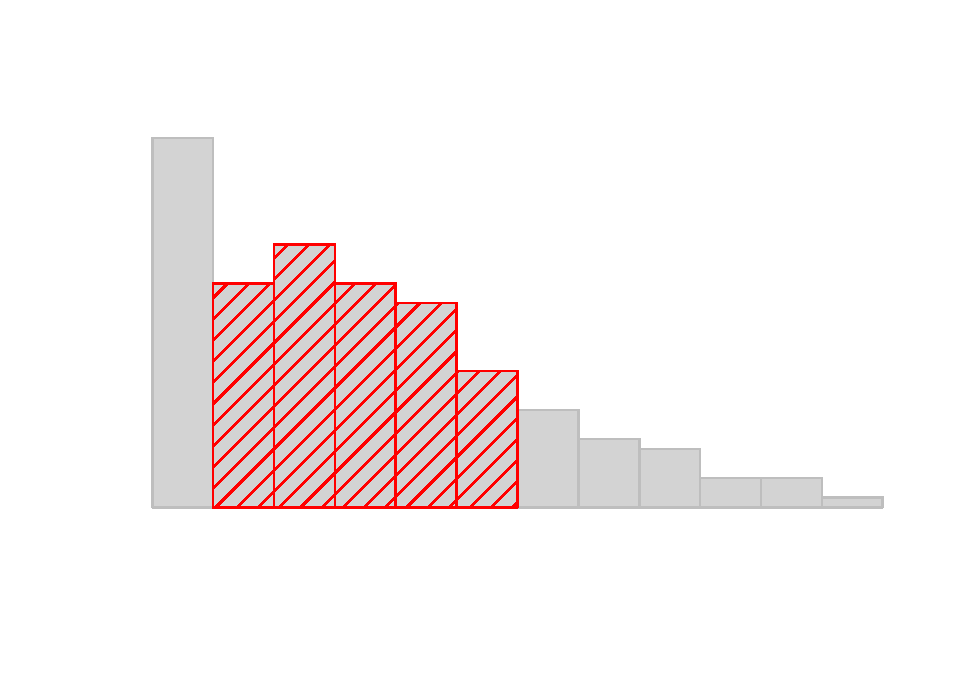
\includegraphics{schuster-statistics-remix_files/figure-latex/aflsd-1.pdf}
\caption{\label{fig:aflsd}An illustration of the standard deviation, applied to the AFL winning margins data. The shaded bars in the histogram show how much of the data fall within one standard deviation of the mean. In this case, 65.3\% of the data set lies within this range, which is pretty consistent with the ``approximately 68\% rule'' discussed in the main text.}
\end{figure}

\hypertarget{mad}{%
\subsection{Median absolute deviation}\label{mad}}

The last measure of variability that I want to talk about is the \textbf{\emph{median absolute deviation}} (MAD). The basic idea behind MAD is very simple, and is pretty much identical to the idea behind the mean absolute deviation (Section \ref{aad}). The difference is that you use the median everywhere. If we were to frame this idea as a pair of R commands, they would look like this:

\begin{Shaded}
\begin{Highlighting}[]
\CommentTok{\# mean absolute deviation from the mean:}
\FunctionTok{mean}\NormalTok{( }\FunctionTok{abs}\NormalTok{(afl.margins }\SpecialCharTok{{-}} \FunctionTok{mean}\NormalTok{(afl.margins)) )}
\end{Highlighting}
\end{Shaded}

\begin{verbatim}
## [1] 21.10124
\end{verbatim}

\begin{Shaded}
\begin{Highlighting}[]
\CommentTok{\# *median* absolute deviation from the *median*:}
\FunctionTok{median}\NormalTok{( }\FunctionTok{abs}\NormalTok{(afl.margins }\SpecialCharTok{{-}} \FunctionTok{median}\NormalTok{(afl.margins)) )}
\end{Highlighting}
\end{Shaded}

\begin{verbatim}
## [1] 19.5
\end{verbatim}

This has a straightforward interpretation: every observation in the data set lies some distance away from the typical value (the median). So the MAD is an attempt to describe a \emph{typical deviation from a typical value} in the data set. It wouldn't be unreasonable to interpret the MAD value of 19.5 for our AFL data by saying something like this:

\begin{quote}
The median winning margin in 2010 was 30.5, indicating that a typical game involved a winning margin of about 30 points. However, there was a fair amount of variation from game to game: the MAD value was 19.5, indicating that a typical winning margin would differ from this median value by about 19-20 points.
\end{quote}

As you'd expect, R has a built in function for calculating MAD, and you will be shocked no doubt to hear that it's called \texttt{mad()}. However, it's a little bit more complicated than the functions that we've been using previously. If you want to use it to calculate MAD in the exact same way that I have described it above, the command that you need to use specifies two arguments: the data set itself \texttt{x}, and a \texttt{constant} that I'll explain in a moment. For our purposes, the constant is 1, so our command becomes

\begin{Shaded}
\begin{Highlighting}[]
\FunctionTok{mad}\NormalTok{( }\AttributeTok{x =}\NormalTok{ afl.margins, }\AttributeTok{constant =} \DecValTok{1}\NormalTok{ )}
\end{Highlighting}
\end{Shaded}

\begin{verbatim}
## [1] 19.5
\end{verbatim}

Apart from the weirdness of having to type that \texttt{constant\ =\ 1} part, this is pretty straightforward.

Okay, so what exactly is this \texttt{constant\ =\ 1} argument? I won't go into all the details here, but here's the gist. Although the ``raw'' MAD value that I've described above is completely interpretable on its own terms, that's not actually how it's used in a lot of real world contexts. Instead, what happens a lot is that the researcher \emph{actually} wants to calculate the standard deviation. However, in the same way that the mean is very sensitive to extreme values, the standard deviation is vulnerable to the exact same issue. So, in much the same way that people sometimes use the median as a ``robust'' way of calculating ``something that is like the mean'', it's not uncommon to use MAD as a method for calculating ``something that is like the standard deviation''. Unfortunately, the \emph{raw} MAD value doesn't do this. Our raw MAD value is 19.5, and our standard deviation was 26.07. However, what some clever person has shown is that, under certain assumptions\footnote{The assumption again being that the data are normally-distributed!}, you can multiply the raw MAD value by 1.4826 and obtain a number that is directly comparable to the standard deviation. As a consequence, the default value of \texttt{constant} is 1.4826, and so when you use the \texttt{mad()} command without manually setting a value, here's what you get:

\begin{Shaded}
\begin{Highlighting}[]
\FunctionTok{mad}\NormalTok{( afl.margins )}
\end{Highlighting}
\end{Shaded}

\begin{verbatim}
## [1] 28.9107
\end{verbatim}

I should point out, though, that if you want to use this ``corrected'' MAD value as a robust version of the standard deviation, you really are relying on the assumption that the data are (or at least, are ``supposed to be'' in some sense) symmetric and basically shaped like a bell curve. That's really \emph{not} true for our \texttt{afl.margins} data, so in this case I wouldn't try to use the MAD value this way.

\hypertarget{which-measure-to-use}{%
\subsection{Which measure to use?}\label{which-measure-to-use}}

We've discussed quite a few measures of spread (range, IQR, MAD, variance and standard deviation), and hinted at their strengths and weaknesses. Here's a quick summary:

\begin{itemize}
\tightlist
\item
  \emph{Range}. Gives you the full spread of the data. It's very vulnerable to outliers, and as a consequence it isn't often used unless you have good reasons to care about the extremes in the data.
\item
  \emph{Interquartile range}. Tells you where the ``middle half'' of the data sits. It's pretty robust, and complements the median nicely. This is used a lot.
\item
  \emph{Mean absolute deviation}. Tells you how far ``on average'' the observations are from the mean. It's very interpretable, but has a few minor issues (not discussed here) that make it less attractive to statisticians than the standard deviation. Used sometimes, but not often.
\item
  \emph{Variance}. Tells you the average squared deviation from the mean. It's mathematically elegant, and is probably the ``right'' way to describe variation around the mean, but it's completely uninterpretable because it doesn't use the same units as the data. Almost never used except as a mathematical tool; but it's buried ``under the hood'' of a very large number of statistical tools.
\item
  \emph{Standard deviation}. This is the square root of the variance. It's fairly elegant mathematically, and it's expressed in the same units as the data so it can be interpreted pretty well. In situations where the mean is the measure of central tendency, this is the default. This is by far the most popular measure of variation.
\item
  \emph{Median absolute deviation}. The typical (i.e., median) deviation from the median value. In the raw form it's simple and interpretable; in the corrected form it's a robust way to estimate the standard deviation, for some kinds of data sets. Not used very often, but it does get reported sometimes.
\end{itemize}

In short, the IQR and the standard deviation are easily the two most common measures used to report the variability of the data; but there are situations in which the others are used. I've described all of them in this book because there's a fair chance you'll run into most of these somewhere.

\hypertarget{skewandkurtosis}{%
\section{Skew and kurtosis}\label{skewandkurtosis}}

Text by David Schuster

There are two more descriptive statistics that you will sometimes see reported in the psychological literature, known as skew and kurtosis. These two measures are useful to diagnose normality (although kurtosis is less useful, in practice). If we find evidence of skewness or kurtosis, we may suspect that our distribution is not normal. Later in this course, we will see that it is generally not a problem for us if one of our sample distributions are non-normal. Regardless, skewness and kurtosis can tell us about the shape of our data.

Example by \citet{Navarro2018}

\begin{verbatim}
## [1] -0.9136909
\end{verbatim}

\begin{verbatim}
## [1] 0.004967443
\end{verbatim}

\begin{figure}
\centering
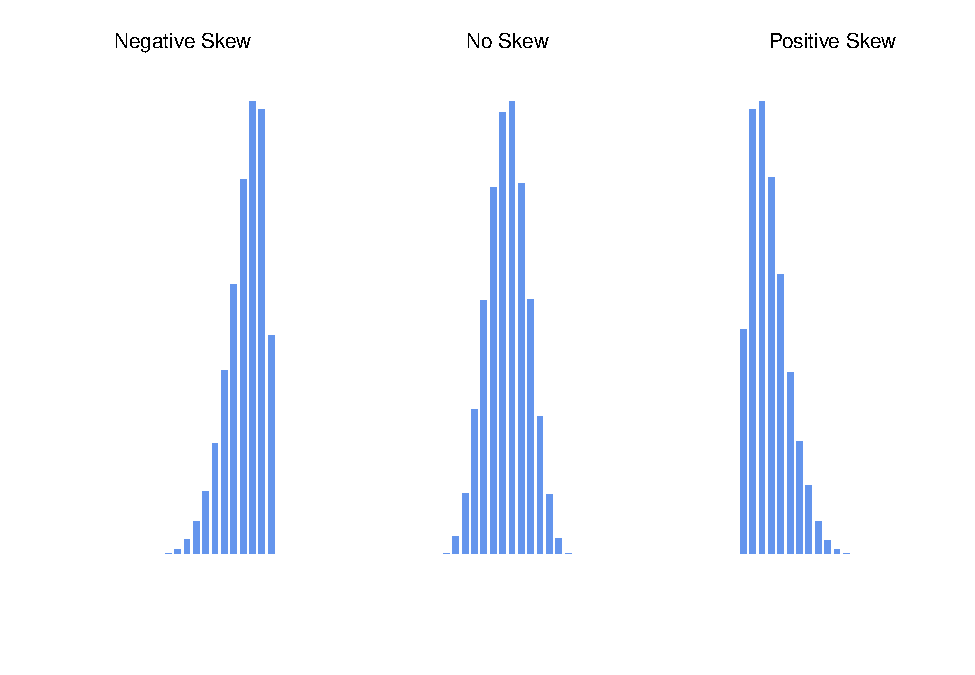
\includegraphics{schuster-statistics-remix_files/figure-latex/skewness-1.pdf}
\caption{\label{fig:skewness}An illustration of skewness. On the left we have a negatively skewed data set (skewness \(= -.93\)), in the middle we have a data set with no skew (technically, skewness \(= -.006\)), and on the right we have a positively skewed data set (skewness \(= .93\)).}
\end{figure}

\begin{verbatim}
## [1] 0.9130693
\end{verbatim}

Since it's the more interesting of the two, let's start by talking about the \textbf{\emph{skewness}}. Skewness is basically a measure of asymmetry, and the easiest way to explain it is by drawing some pictures. As Figure \ref{fig:skewness} illustrates, if the data tend to have a lot of extreme small values (i.e., the lower tail is ``longer'' than the upper tail) and not so many extremely large values (left panel), then we say that the data are \emph{negatively skewed}. On the other hand, if there are more extremely large values than extremely small ones (right panel) we say that the data are \emph{positively skewed}. That's the qualitative idea behind skewness. The actual formula for the skewness of a data set is as follows
\[
\mbox{skewness}(X) = \frac{1}{N \hat{\sigma}^3} \sum_{i=1}^N (X_i - \bar{X})^3
\]
where \(N\) is the number of observations, \(\bar{X}\) is the sample mean, and \(\hat{\sigma}\) is the standard deviation (the ``divide by \(N-1\)'' version, that is). Perhaps more helpfully, it might be useful to point out that the \texttt{psych} package contains a \texttt{skew()} function that you can use to calculate skewness. So if we wanted to use this function to calculate the skewness of the \texttt{afl.margins} data, we'd first need to load the package

\begin{Shaded}
\begin{Highlighting}[]
\FunctionTok{library}\NormalTok{( psych )}
\end{Highlighting}
\end{Shaded}

which now makes it possible to use the following command:

\begin{Shaded}
\begin{Highlighting}[]
\FunctionTok{skew}\NormalTok{( }\AttributeTok{x =}\NormalTok{ afl.margins )}
\end{Highlighting}
\end{Shaded}

\begin{verbatim}
## [1] 0.7671555
\end{verbatim}

Not surprisingly, it turns out that the AFL winning margins data is fairly skewed.

\hypertarget{more-detail-on-skewness-measures}{%
\subsection{More detail on skewness measures}\label{more-detail-on-skewness-measures}}

Text by David Schuster

Unfortunately, this characterization of skewness is a bit of a simplification. R's \emph{psych} package does have a skewness statistic, but it does not match the formula Navarro provided in this section. I spent an afternoon disentangling all the available skewness statistics. Rather than get too detailed with this (if you want that detail, look for Doane \& Seward's 2011 article on measuring skewness), allow me to summarize:

\begin{itemize}
\item
  First, my overall recommendation would be to visually examine a Q-Q plot and histogram, then run a Shapiro-Wilks test, understanding that none of these methods are perfect.
\item
  Skewness is defined mathematically as the third \textbf{moment}. Moments are statistical parameters. The first moment is mean, the second moment is variance, the third moment is skewness, and the fourth moment is kurtosis
\item
  The mathematical definition is of limited use to the researcher, because it does not account for sample size or variation in samples (sampling error)
\item
  Statisticians have come up with several more useful measures of skewness. Their performance differences are not very important in practice, and they tend to give the same result when you have large samples.
\item
  It matters less which skewness value you report. It is more important that you are clear about which statistic you used. Frustratingly, stats packages and Excel implement a single method but do not make it clear which method they use. This leads to people saying, ``I measured skewness using SPSS,'' which the SPSS people probably really like.
\item
  For future reference more than use right now, I researched which measures are used in which packages.
\end{itemize}

\hypertarget{use-statistics-to-describe-skew}{%
\subsubsection{Use statistics to describe skew}\label{use-statistics-to-describe-skew}}

\begin{Shaded}
\begin{Highlighting}[]
\NormalTok{x }\OtherTok{\textless{}{-}}\NormalTok{ afl.margins }\CommentTok{\# use the same example}
\NormalTok{n }\OtherTok{\textless{}{-}} \FunctionTok{length}\NormalTok{(x) }\CommentTok{\# sample size}
\NormalTok{sum\_cubed }\OtherTok{\textless{}{-}} \FunctionTok{sum}\NormalTok{((x }\SpecialCharTok{{-}} \FunctionTok{mean}\NormalTok{(x))}\SpecialCharTok{\^{}}\DecValTok{3}\NormalTok{) }\CommentTok{\# sum of cubed deviations from the mean}
\NormalTok{pop\_sd }\OtherTok{\textless{}{-}} \FunctionTok{sqrt}\NormalTok{(}\FunctionTok{var}\NormalTok{(x) }\SpecialCharTok{*}\NormalTok{ (n}\DecValTok{{-}1}\NormalTok{)}\SpecialCharTok{/}\NormalTok{n) }\CommentTok{\# population sd}
\NormalTok{sample\_sd }\OtherTok{\textless{}{-}} \FunctionTok{sd}\NormalTok{(x)}
\NormalTok{pop\_sd\_cubed }\OtherTok{\textless{}{-}}\NormalTok{ pop\_sd}\SpecialCharTok{\^{}}\DecValTok{3} \CommentTok{\# population sd cubed}

\NormalTok{gamma\_1 }\OtherTok{\textless{}{-}}\NormalTok{ sum\_cubed }\SpecialCharTok{/}\NormalTok{ pop\_sd\_cubed  }\CommentTok{\# Pearson’s moment coefficient of skewness}
\NormalTok{g\_1 }\OtherTok{\textless{}{-}}\NormalTok{ sum\_cubed }\SpecialCharTok{/}\NormalTok{ (pop\_sd\_cubed }\SpecialCharTok{*}\NormalTok{ n) }\CommentTok{\# Fisher{-}Pearson coefficient of skewness (Type = 1, Excel skew.p, Cohen (2013), skewness())}
\NormalTok{G\_1 }\OtherTok{\textless{}{-}}\NormalTok{ (n }\SpecialCharTok{/}\NormalTok{ ((n}\DecValTok{{-}1}\NormalTok{)}\SpecialCharTok{*}\NormalTok{(n}\DecValTok{{-}2}\NormalTok{))) }\SpecialCharTok{*} \FunctionTok{sum}\NormalTok{(((x }\SpecialCharTok{{-}} \FunctionTok{mean}\NormalTok{(x)) }\SpecialCharTok{/}\NormalTok{ sample\_sd)}\SpecialCharTok{\^{}}\DecValTok{3}\NormalTok{)  }\CommentTok{\# adjusted Fisher–Pearson standardized moment coefficient (Type = 2, Excel skew, SPSS skew)}
\NormalTok{b\_1 }\OtherTok{\textless{}{-}}\NormalTok{ g\_1 }\SpecialCharTok{*}\NormalTok{ ((n}\DecValTok{{-}1}\NormalTok{)}\SpecialCharTok{/}\NormalTok{n)}\SpecialCharTok{\^{}}\NormalTok{(}\DecValTok{3}\SpecialCharTok{/}\DecValTok{2}\NormalTok{) }\CommentTok{\# (Type = 3, MINITAB, stat.desc, skew(), psych package)}
\NormalTok{SE\_skew\_SPSS }\OtherTok{=} \FunctionTok{sqrt}\NormalTok{(}\DecValTok{6}\SpecialCharTok{*}\NormalTok{n}\SpecialCharTok{*}\NormalTok{(n}\DecValTok{{-}1}\NormalTok{) }\SpecialCharTok{/}\NormalTok{ ((n}\DecValTok{{-}2}\NormalTok{)}\SpecialCharTok{*}\NormalTok{(n}\SpecialCharTok{+}\DecValTok{1}\NormalTok{)}\SpecialCharTok{*}\NormalTok{(n}\SpecialCharTok{+}\DecValTok{3}\NormalTok{))) }\CommentTok{\# SPSS skewness SE per https://www.ibm.com/support/pages/standard{-}errors{-}skewness{-}and{-}kurtosis{-}are{-}all{-}same{-}set{-}variables}

\NormalTok{gamma\_1}
\end{Highlighting}
\end{Shaded}

\begin{verbatim}
## [1] 136.1783
\end{verbatim}

\begin{Shaded}
\begin{Highlighting}[]
\NormalTok{g\_1}
\end{Highlighting}
\end{Shaded}

\begin{verbatim}
## [1] 0.7737405
\end{verbatim}

\begin{Shaded}
\begin{Highlighting}[]
\NormalTok{G\_1}
\end{Highlighting}
\end{Shaded}

\begin{verbatim}
## [1] 0.7804075
\end{verbatim}

\begin{Shaded}
\begin{Highlighting}[]
\NormalTok{b\_1}
\end{Highlighting}
\end{Shaded}

\begin{verbatim}
## [1] 0.7671555
\end{verbatim}

The point of all of this is to be aware that when you use the psych package and skew() or stat.desc commands, you are reporting \(\beta_{1}\). SPSS reports \(G_{1}\) as the skewness statistic as well as a standard error statisti. You can replicate this, if you want:

\begin{enumerate}
\def\labelenumi{\arabic{enumi}.}
\item
  Find \(G_{1}\) using \texttt{skew(x,\ type\ =\ 2)}
\item
  Find \({SE_{skew}}\) using the R formula: \texttt{sqrt(6*n*(n-1)\ /\ ((n-2)*(n+1)*(n+3)))}
\item
  Divide: \(G_{1}/{SE_{skew}}\).
\item
  If the result is between -2 and 2, you can infer a lack of skewness. Values -2 indicate a concerning amount of negative skew; values above 2 indicate a concerning amount of positive skew.
\end{enumerate}

\hypertarget{examine-the-histogram}{%
\subsubsection{Examine the histogram}\label{examine-the-histogram}}

\begin{Shaded}
\begin{Highlighting}[]
\FunctionTok{hist}\NormalTok{(x)}
\end{Highlighting}
\end{Shaded}

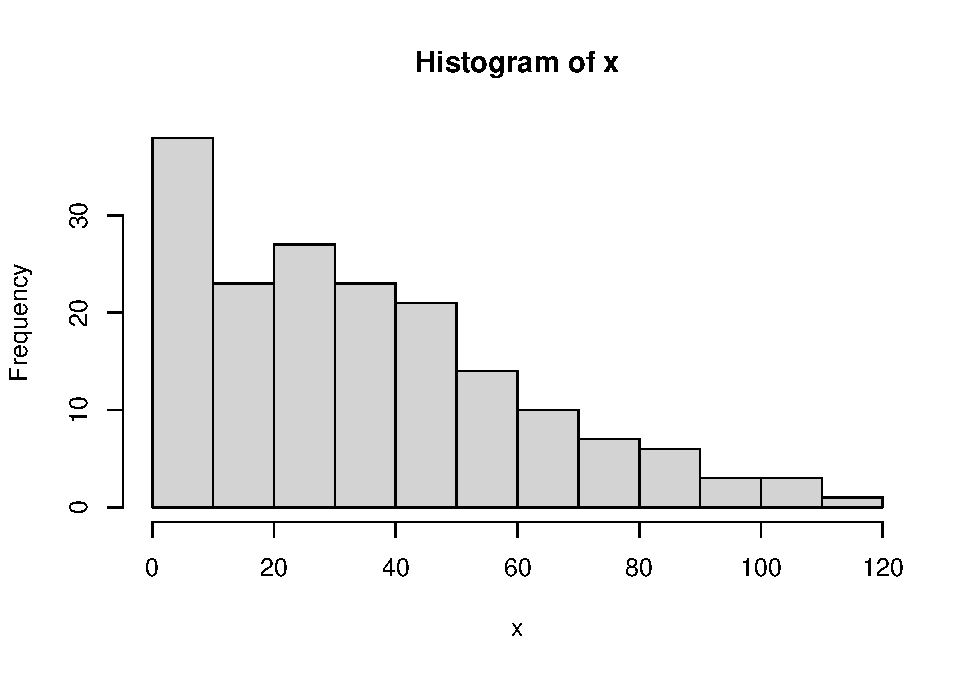
\includegraphics{schuster-statistics-remix_files/figure-latex/unnamed-chunk-207-1.pdf}

\hypertarget{look-for-normality-visually-in-a-q-q-plot-quantile-quantile-plot}{%
\subsubsection{Look for normality visually in a Q-Q plot (quantile-quantile plot)}\label{look-for-normality-visually-in-a-q-q-plot-quantile-quantile-plot}}

\begin{Shaded}
\begin{Highlighting}[]
\FunctionTok{library}\NormalTok{(}\StringTok{"ggplot2"}\NormalTok{)}
\end{Highlighting}
\end{Shaded}

\begin{verbatim}
## 
## Attaching package: 'ggplot2'
\end{verbatim}

\begin{verbatim}
## The following objects are masked from 'package:psych':
## 
##     %+%, alpha
\end{verbatim}

\begin{Shaded}
\begin{Highlighting}[]
\FunctionTok{qplot}\NormalTok{(}\AttributeTok{sample =}\NormalTok{ x) }\CommentTok{\# qplot Q{-}Q plots}
\end{Highlighting}
\end{Shaded}

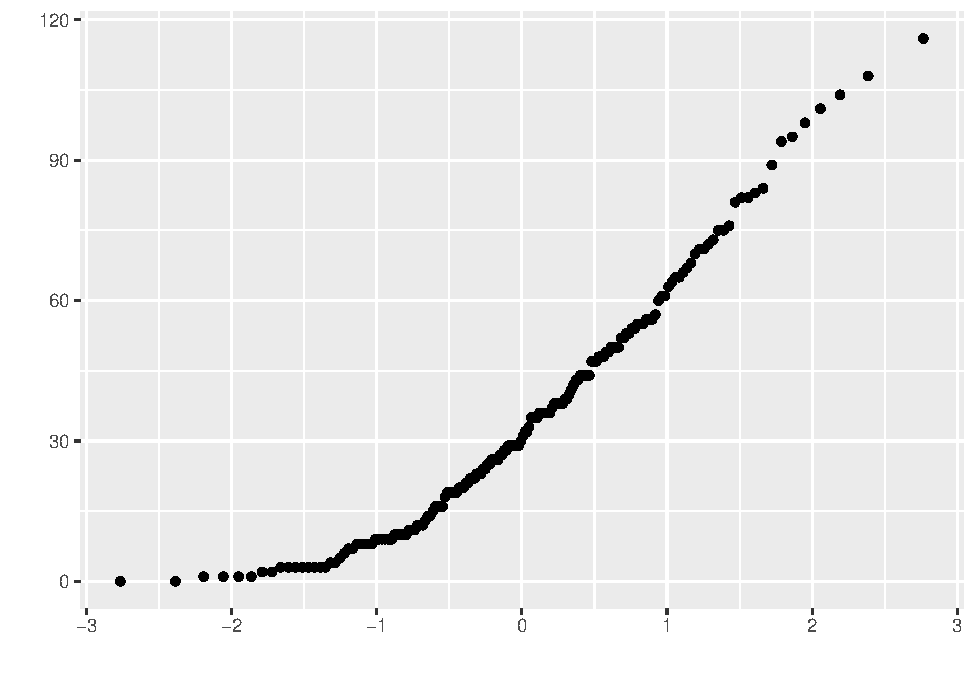
\includegraphics{schuster-statistics-remix_files/figure-latex/unnamed-chunk-208-1.pdf}

\begin{itemize}
\item
  In a normal distribution, the dots of the plot will form a near-straight line.
\item
  Remember that quantiles divide a continuous probability distribution into intervals with equal probabilities.
\item
  A Q-Q plot is based on quantiles of data versus theoretical normal distribution.
\item
  In contrast a P-P plot (not shown here) is based on the cumulative density function (probability) of data versus a theoretical normal distribution.
\item
  Q-Q is better at detecting differences near the middle of the distribution than a P-P plot.
\end{itemize}

\hypertarget{the-shapiro-wilk-test-tests-the-null-hypothsis-that-data-are-from-a-normal-distribution}{%
\subsubsection{The Shapiro-Wilk test tests the null hypothsis that data are from a normal distribution}\label{the-shapiro-wilk-test-tests-the-null-hypothsis-that-data-are-from-a-normal-distribution}}

If p \textless{} .05, reject the null and conclude the data are not normal. If p \textgreater{} .05, retain the null and officially make no inference about the distribution. Also, beware that not all deviations from normality may be detected, and, in large samples, the test may be too sensitive. Report as \emph{W}(df) = \#, p = \#.

\begin{Shaded}
\begin{Highlighting}[]
\FunctionTok{shapiro.test}\NormalTok{(x) }
\end{Highlighting}
\end{Shaded}

\begin{verbatim}
## 
##  Shapiro-Wilk normality test
## 
## data:  x
## W = 0.9398, p-value = 9.481e-07
\end{verbatim}

The final measure that is sometimes referred to, though very rarely in practice, is the \textbf{\emph{kurtosis}} of a data set. Put simply, kurtosis is a measure of the ``pointiness'' of a data set, as illustrated in Figure \ref{fig:kurtosis}.

\begin{verbatim}
## [1] -0.9560784
\end{verbatim}

\begin{verbatim}
## [1] -0.01663342
\end{verbatim}

\begin{figure}
\centering
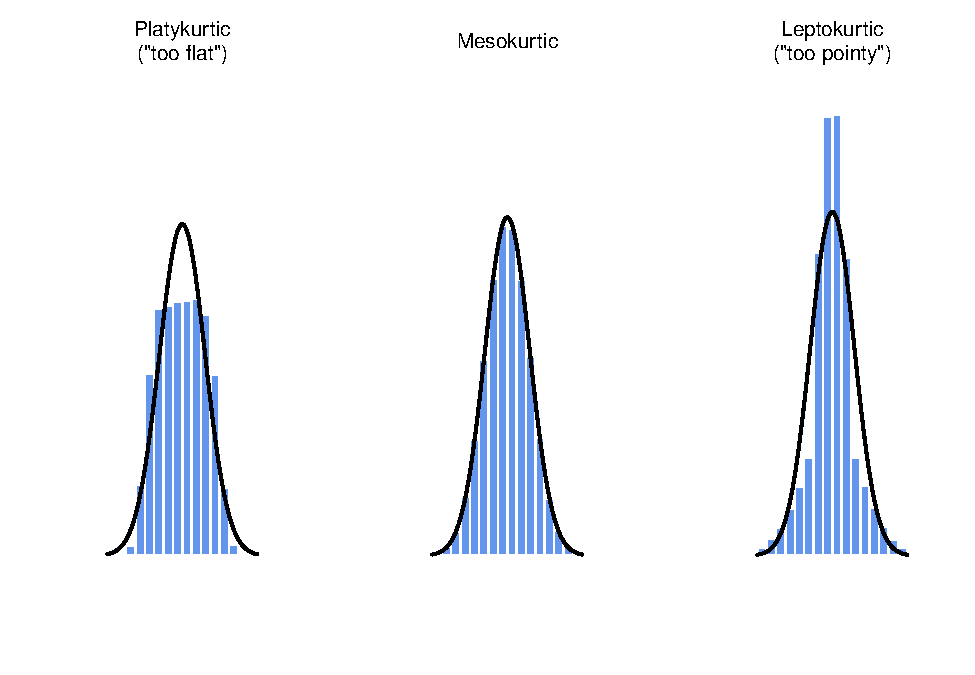
\includegraphics{schuster-statistics-remix_files/figure-latex/kurtosis-1.pdf}
\caption{\label{fig:kurtosis}An illustration of kurtosis. On the left, we have a ``platykurtic'' data set (kurtosis = \(-.95\)), meaning that the data set is ``too flat''. In the middle we have a ``mesokurtic'' data set (kurtosis is almost exactly 0), which means that the pointiness of the data is just about right. Finally, on the right, we have a ``leptokurtic'' data set (kurtosis \(= 2.12\)) indicating that the data set is ``too pointy''. Note that kurtosis is measured with respect to a normal curve (black line)}
\end{figure}

\begin{verbatim}
## [1] 1.975364
\end{verbatim}

By convention, we say that the ``normal curve'' (black lines) has zero kurtosis, so the pointiness of a data set is assessed relative to this curve. In this Figure, the data on the left are not pointy enough, so the kurtosis is negative and we call the data \emph{platykurtic}. The data on the right are too pointy, so the kurtosis is positive and we say that the data is \emph{leptokurtic}. But the data in the middle are just pointy enough, so we say that it is \emph{mesokurtic} and has kurtosis zero. This is summarised in the table below:

\begin{tabular}{lll}
\toprule
informal term & technical name & kurtosis value\\
\midrule
too flat & platykurtic & negative\\
just pointy enough & mesokurtic & zero\\
too pointy & leptokurtic & positive\\
\bottomrule
\end{tabular}

The equation for kurtosis is pretty similar in spirit to the formulas we've seen already for the variance and the skewness; except that where the variance involved squared deviations and the skewness involved cubed deviations, the kurtosis involves raising the deviations to the fourth power:\footnote{The ``\(-3\)'' part is something that statisticians tack on to ensure that the normal curve has kurtosis zero. It looks a bit stupid, just sticking a ``-3'' at the end of the formula, but there are good mathematical reasons for doing this.}
\[
\mbox{kurtosis}(X) = \frac{1}{N \hat\sigma^4} \sum_{i=1}^N \left( X_i - \bar{X} \right)^4  - 3
\]
I know, it's not terribly interesting to me either. More to the point, the \texttt{psych} package has a function called \texttt{kurtosi()} that you can use to calculate the kurtosis of your data. For instance, if we were to do this for the AFL margins,

\begin{Shaded}
\begin{Highlighting}[]
\FunctionTok{kurtosi}\NormalTok{( }\AttributeTok{x =}\NormalTok{ afl.margins )}
\end{Highlighting}
\end{Shaded}

\begin{verbatim}
## [1] 0.02962633
\end{verbatim}

we discover that the AFL winning margins data are just pointy enough.

\hypertarget{descriptive-summary}{%
\section{Getting an overall summary of a variable}\label{descriptive-summary}}

Up to this point in the chapter I've explained several different summary statistics that are commonly used when analysing data, along with specific functions that you can use in R to calculate each one. However, it's kind of annoying to have to separately calculate means, medians, standard deviations, skews etc. Wouldn't it be nice if R had some helpful functions that would do all these tedious calculations at once? Something like \texttt{summary()} or \texttt{describe()}, perhaps? Why yes, yes it would. So much so that both of these functions exist. The \texttt{summary()} function is in the \texttt{base} package, so it comes with every installation of R. The \texttt{describe()} function is part of the \texttt{psych} package, which we loaded earlier in the chapter.

\hypertarget{summarising-a-variable}{%
\subsection{``Summarising'' a variable}\label{summarising-a-variable}}

The \texttt{summary()} function is an easy thing to use, but a tricky thing to understand in full, since it's a generic function (see Section \ref{generics}. The basic idea behind the \texttt{summary()} function is that it prints out some useful information about whatever object (i.e., variable, as far as we're concerned) you specify as the \texttt{object} argument. As a consequence, the behaviour of the \texttt{summary()} function differs quite dramatically depending on the class of the object that you give it. Let's start by giving it a \emph{numeric} object:

\begin{Shaded}
\begin{Highlighting}[]
\FunctionTok{summary}\NormalTok{( }\AttributeTok{object =}\NormalTok{ afl.margins )  }
\end{Highlighting}
\end{Shaded}

\begin{verbatim}
##    Min. 1st Qu.  Median    Mean 3rd Qu.    Max. 
##    0.00   12.75   30.50   35.30   50.50  116.00
\end{verbatim}

For numeric variables, we get a whole bunch of useful descriptive statistics. It gives us the minimum and maximum values (i.e., the range), the first and third quartiles (25th and 75th percentiles; i.e., the IQR), the mean and the median. In other words, it gives us a pretty good collection of descriptive statistics related to the central tendency and the spread of the data.

Okay, what about if we feed it a logical vector instead? Let's say I want to know something about how many ``blowouts'' there were in the 2010 AFL season. I operationalise the concept of a blowout (see Chapter \ref{studydesign}) as a game in which the winning margin exceeds 50 points. Let's create a logical variable \texttt{blowouts} in which the \(i\)-th element is \texttt{TRUE} if that game was a blowout according to my definition,

\begin{Shaded}
\begin{Highlighting}[]
\NormalTok{blowouts }\OtherTok{\textless{}{-}}\NormalTok{  afl.margins }\SpecialCharTok{\textgreater{}} \DecValTok{50}
\NormalTok{blowouts}
\end{Highlighting}
\end{Shaded}

\begin{verbatim}
##   [1]  TRUE FALSE  TRUE FALSE FALSE FALSE FALSE  TRUE FALSE FALSE FALSE
##  [12]  TRUE FALSE FALSE  TRUE FALSE FALSE FALSE FALSE  TRUE FALSE FALSE
##  [23] FALSE FALSE FALSE FALSE FALSE  TRUE FALSE  TRUE  TRUE FALSE FALSE
##  [34]  TRUE FALSE FALSE  TRUE FALSE FALSE FALSE FALSE FALSE FALSE FALSE
##  [45] FALSE  TRUE  TRUE FALSE FALSE FALSE FALSE FALSE  TRUE  TRUE FALSE
##  [56]  TRUE FALSE FALSE FALSE FALSE  TRUE FALSE FALSE FALSE FALSE FALSE
##  [67]  TRUE FALSE FALSE FALSE FALSE FALSE FALSE  TRUE FALSE FALSE FALSE
##  [78] FALSE FALSE  TRUE FALSE FALSE FALSE FALSE FALSE FALSE FALSE FALSE
##  [89] FALSE FALSE  TRUE FALSE FALSE  TRUE FALSE FALSE FALSE FALSE FALSE
## [100] FALSE  TRUE FALSE FALSE FALSE  TRUE FALSE  TRUE  TRUE  TRUE FALSE
## [111] FALSE FALSE FALSE FALSE FALSE FALSE FALSE FALSE FALSE  TRUE FALSE
## [122]  TRUE FALSE FALSE FALSE FALSE FALSE FALSE FALSE  TRUE  TRUE FALSE
## [133] FALSE  TRUE  TRUE FALSE FALSE FALSE FALSE FALSE  TRUE FALSE  TRUE
## [144]  TRUE  TRUE  TRUE FALSE FALSE FALSE  TRUE FALSE FALSE  TRUE FALSE
## [155]  TRUE FALSE  TRUE FALSE FALSE  TRUE FALSE FALSE  TRUE FALSE FALSE
## [166] FALSE FALSE FALSE FALSE FALSE FALSE FALSE FALSE FALSE FALSE FALSE
\end{verbatim}

So that's what the \texttt{blowouts} variable looks like. Now let's ask R for a \texttt{summary()}

\begin{Shaded}
\begin{Highlighting}[]
\FunctionTok{summary}\NormalTok{( }\AttributeTok{object =}\NormalTok{ blowouts )}
\end{Highlighting}
\end{Shaded}

\begin{verbatim}
##    Mode   FALSE    TRUE 
## logical     132      44
\end{verbatim}

In this context, the \texttt{summary()} function gives us a count of the number of \texttt{TRUE} values, the number of \texttt{FALSE} values, and the number of missing values (i.e., the \texttt{NA}s). Pretty reasonable behaviour.

Next, let's try to give it a factor. If you recall, I've defined the \texttt{afl.finalists} vector as a factor, so let's use that:

\begin{Shaded}
\begin{Highlighting}[]
\FunctionTok{summary}\NormalTok{( }\AttributeTok{object =}\NormalTok{ afl.finalists )}
\end{Highlighting}
\end{Shaded}

\begin{verbatim}
##         Adelaide         Brisbane          Carlton      Collingwood 
##               26               25               26               28 
##         Essendon          Fitzroy        Fremantle          Geelong 
##               32                0                6               39 
##         Hawthorn        Melbourne  North Melbourne    Port Adelaide 
##               27               28               28               17 
##         Richmond         St Kilda           Sydney       West Coast 
##                6               24               26               38 
## Western Bulldogs 
##               24
\end{verbatim}

For factors, we get a frequency table, just like we got when we used the \texttt{table()} function. Interestingly, however, if we convert this to a character vector using the \texttt{as.character()} function (see Section \ref{coercion}, we don't get the same results:

\begin{Shaded}
\begin{Highlighting}[]
\NormalTok{f2 }\OtherTok{\textless{}{-}} \FunctionTok{as.character}\NormalTok{( afl.finalists )}
\FunctionTok{summary}\NormalTok{( }\AttributeTok{object =}\NormalTok{ f2 )}
\end{Highlighting}
\end{Shaded}

\begin{verbatim}
##    Length     Class      Mode 
##       400 character character
\end{verbatim}

This is one of those situations I was referring to in Section \ref{factors}, in which it is helpful to declare your nominal scale variable as a factor rather than a character vector. Because I've defined \texttt{afl.finalists} as a factor, R \emph{knows} that it should treat it as a nominal scale variable, and so it gives you a much more detailed (and helpful) summary than it would have if I'd left it as a character vector.

\hypertarget{summarising-a-data-frame}{%
\subsection{``Summarising'' a data frame}\label{summarising-a-data-frame}}

Okay what about data frames? When you pass a data frame to the \texttt{summary()} function, it produces a slightly condensed summary of each variable inside the data frame. To give you a sense of how this can be useful, let's try this for a new data set, one that you've never seen before. The data is stored in the \texttt{clinicaltrial.Rdata} file, and we'll use it a lot in Chapter \ref{anova} (you can find a complete description of the data at the start of that chapter). Let's load it, and see what we've got:

\begin{Shaded}
\begin{Highlighting}[]
\FunctionTok{load}\NormalTok{( }\StringTok{"./data/clinicaltrial.Rdata"}\NormalTok{ )}
\FunctionTok{who}\NormalTok{(}\ConstantTok{TRUE}\NormalTok{)}
\end{Highlighting}
\end{Shaded}

\begin{verbatim}
##    -- Name --    -- Class --   -- Size --
##    clin.trial    data.frame    18 x 3    
##     $drug        factor        18        
##     $therapy     factor        18        
##     $mood.gain   numeric       18
\end{verbatim}

There's a single data frame called \texttt{clin.trial} which contains three variables, \texttt{drug}, \texttt{therapy} and \texttt{mood.gain}. Presumably then, this data is from a clinical trial of some kind, in which people were administered different drugs; and the researchers looked to see what the drugs did to their mood. Let's see if the \texttt{summary()} function sheds a little more light on this situation:

\begin{Shaded}
\begin{Highlighting}[]
\FunctionTok{summary}\NormalTok{( clin.trial )}
\end{Highlighting}
\end{Shaded}

\begin{verbatim}
##        drug         therapy    mood.gain     
##  placebo :6   no.therapy:9   Min.   :0.1000  
##  anxifree:6   CBT       :9   1st Qu.:0.4250  
##  joyzepam:6                  Median :0.8500  
##                              Mean   :0.8833  
##                              3rd Qu.:1.3000  
##                              Max.   :1.8000
\end{verbatim}

Evidently there were three drugs: a placebo, something called ``anxifree'' and something called ``joyzepam''; and there were 6 people administered each drug. There were 9 people treated using cognitive behavioural therapy (CBT) and 9 people who received no psychological treatment. And we can see from looking at the summary of the \texttt{mood.gain} variable that most people did show a mood gain (mean \(=.88\)), though without knowing what the scale is here it's hard to say much more than that. Still, that's not too bad. Overall, I feel that I learned something from that.

\hypertarget{describing-a-data-frame}{%
\subsection{``Describing'' a data frame}\label{describing-a-data-frame}}

The \texttt{describe()} function (in the \texttt{psych} package) is a little different, and it's really only intended to be useful when your data are interval or ratio scale. Unlike the \texttt{summary()} function, it calculates the same descriptive statistics for any type of variable you give it. By default, these are:

\begin{itemize}
\tightlist
\item
  \texttt{var}. This is just an index: 1 for the first variable, 2 for the second variable, and so on.
\item
  \texttt{n}. This is the sample size: more precisely, it's the number of non-missing values.
\item
  \texttt{mean}. This is the sample mean (Section \ref{mean}).
\item
  \texttt{sd}. This is the (bias corrected) standard deviation (Section \ref{sd}).
\item
  \texttt{median}. The median (Section \ref{median}).
\item
  \texttt{trimmed}. This is trimmed mean. By default it's the 10\% trimmed mean (Section \ref{trimmedmean}).
\item
  \texttt{mad}. The median absolute deviation (Section \ref{mad}).
\item
  \texttt{min}. The minimum value.
\item
  \texttt{max}. The maximum value.
\item
  \texttt{range}. The range spanned by the data (Section \ref{range}).
\item
  \texttt{skew}. The skewness (Section \ref{skewandkurtosis}).
\item
  \texttt{kurtosis}. The kurtosis (Section \ref{skewandkurtosis}).
\item
  \texttt{se}. The standard error of the mean (Chapter \ref{estimation}).
\end{itemize}

Notice that these descriptive statistics generally only make sense for data that are interval or ratio scale (usually encoded as numeric vectors). For nominal or ordinal variables (usually encoded as factors), most of these descriptive statistics are not all that useful. What the \texttt{describe()} function does is convert factors and logical variables to numeric vectors in order to do the calculations. These variables are marked with \texttt{*} and most of the time, the descriptive statistics for those variables won't make much sense. If you try to feed it a data frame that includes a character vector as a variable, it produces an error.

With those caveats in mind, let's use the \texttt{describe()} function to have a look at the \texttt{clin.trial} data frame. Here's what we get:

\begin{Shaded}
\begin{Highlighting}[]
\FunctionTok{describe}\NormalTok{( }\AttributeTok{x =}\NormalTok{ clin.trial )}
\end{Highlighting}
\end{Shaded}

\begin{verbatim}
##           vars  n mean   sd median trimmed  mad min max range skew
## drug*        1 18 2.00 0.84   2.00    2.00 1.48 1.0 3.0   2.0 0.00
## therapy*     2 18 1.50 0.51   1.50    1.50 0.74 1.0 2.0   1.0 0.00
## mood.gain    3 18 0.88 0.53   0.85    0.88 0.67 0.1 1.8   1.7 0.13
##           kurtosis   se
## drug*        -1.66 0.20
## therapy*     -2.11 0.12
## mood.gain    -1.44 0.13
\end{verbatim}

As you can see, the output for the asterisked variables is pretty meaningless, and should be ignored. However, for the \texttt{mood.gain} variable, there's a lot of useful information.

\hypertarget{groupdescriptives}{%
\section{Descriptive statistics separately for each group}\label{groupdescriptives}}

It is very commonly the case that you find yourself needing to look at descriptive statistics, broken down by some grouping variable. This is pretty easy to do in R, and there are three functions in particular that are worth knowing about: \texttt{by()}, \texttt{describeBy()} and \texttt{aggregate()}. Let's start with the \texttt{describeBy()} function, which is part of the \texttt{psych} package. The \texttt{describeBy()} function is very similar to the \texttt{describe()} function, except that it has an additional argument called \texttt{group} which specifies a grouping variable. For instance, let's say, I want to look at the descriptive statistics for the \texttt{clin.trial} data, broken down separately by \texttt{therapy} type. The command I would use here is:

\begin{Shaded}
\begin{Highlighting}[]
\FunctionTok{describeBy}\NormalTok{( }\AttributeTok{x=}\NormalTok{clin.trial, }\AttributeTok{group=}\NormalTok{clin.trial}\SpecialCharTok{$}\NormalTok{therapy )}
\end{Highlighting}
\end{Shaded}

\begin{verbatim}
## 
##  Descriptive statistics by group 
## group: no.therapy
##           vars n mean   sd median trimmed  mad min max range skew kurtosis
## drug*        1 9 2.00 0.87    2.0    2.00 1.48 1.0 3.0   2.0 0.00    -1.81
## therapy*     2 9 1.00 0.00    1.0    1.00 0.00 1.0 1.0   0.0  NaN      NaN
## mood.gain    3 9 0.72 0.59    0.5    0.72 0.44 0.1 1.7   1.6 0.51    -1.59
##             se
## drug*     0.29
## therapy*  0.00
## mood.gain 0.20
## -------------------------------------------------------- 
## group: CBT
##           vars n mean   sd median trimmed  mad min max range  skew
## drug*        1 9 2.00 0.87    2.0    2.00 1.48 1.0 3.0   2.0  0.00
## therapy*     2 9 2.00 0.00    2.0    2.00 0.00 2.0 2.0   0.0   NaN
## mood.gain    3 9 1.04 0.45    1.1    1.04 0.44 0.3 1.8   1.5 -0.03
##           kurtosis   se
## drug*        -1.81 0.29
## therapy*       NaN 0.00
## mood.gain    -1.12 0.15
\end{verbatim}

As you can see, the output is essentially identical to the output that the \texttt{describe()} function produce, except that the output now gives you means, standard deviations etc separately for the \texttt{CBT} group and the \texttt{no.therapy} group. Notice that, as before, the output displays asterisks for factor variables, in order to draw your attention to the fact that the descriptive statistics that it has calculated won't be very meaningful for those variables. Nevertheless, this command has given us some really useful descriptive statistics \texttt{mood.gain} variable, broken down as a function of \texttt{therapy}.

A somewhat more general solution is offered by the \texttt{by()} function. There are three arguments that you need to specify when using this function: the \texttt{data} argument specifies the data set, the \texttt{INDICES} argument specifies the grouping variable, and the \texttt{FUN} argument specifies the name of a function that you want to apply separately to each group. To give a sense of how powerful this is, you can reproduce the \texttt{describeBy()} function by using a command like this:

\begin{Shaded}
\begin{Highlighting}[]
\FunctionTok{by}\NormalTok{( }\AttributeTok{data=}\NormalTok{clin.trial, }\AttributeTok{INDICES=}\NormalTok{clin.trial}\SpecialCharTok{$}\NormalTok{therapy, }\AttributeTok{FUN=}\NormalTok{describe )}
\end{Highlighting}
\end{Shaded}

\begin{verbatim}
## clin.trial$therapy: no.therapy
##           vars n mean   sd median trimmed  mad min max range skew kurtosis
## drug*        1 9 2.00 0.87    2.0    2.00 1.48 1.0 3.0   2.0 0.00    -1.81
## therapy*     2 9 1.00 0.00    1.0    1.00 0.00 1.0 1.0   0.0  NaN      NaN
## mood.gain    3 9 0.72 0.59    0.5    0.72 0.44 0.1 1.7   1.6 0.51    -1.59
##             se
## drug*     0.29
## therapy*  0.00
## mood.gain 0.20
## -------------------------------------------------------- 
## clin.trial$therapy: CBT
##           vars n mean   sd median trimmed  mad min max range  skew
## drug*        1 9 2.00 0.87    2.0    2.00 1.48 1.0 3.0   2.0  0.00
## therapy*     2 9 2.00 0.00    2.0    2.00 0.00 2.0 2.0   0.0   NaN
## mood.gain    3 9 1.04 0.45    1.1    1.04 0.44 0.3 1.8   1.5 -0.03
##           kurtosis   se
## drug*        -1.81 0.29
## therapy*       NaN 0.00
## mood.gain    -1.12 0.15
\end{verbatim}

This will produce the exact same output as the command shown earlier. However, there's nothing special about the \texttt{describe()} function. You could just as easily use the \texttt{by()} function in conjunction with the \texttt{summary()} function. For example:

\begin{Shaded}
\begin{Highlighting}[]
\FunctionTok{by}\NormalTok{( }\AttributeTok{data=}\NormalTok{clin.trial, }\AttributeTok{INDICES=}\NormalTok{clin.trial}\SpecialCharTok{$}\NormalTok{therapy, }\AttributeTok{FUN=}\NormalTok{summary )}
\end{Highlighting}
\end{Shaded}

\begin{verbatim}
## clin.trial$therapy: no.therapy
##        drug         therapy    mood.gain     
##  placebo :3   no.therapy:9   Min.   :0.1000  
##  anxifree:3   CBT       :0   1st Qu.:0.3000  
##  joyzepam:3                  Median :0.5000  
##                              Mean   :0.7222  
##                              3rd Qu.:1.3000  
##                              Max.   :1.7000  
## -------------------------------------------------------- 
## clin.trial$therapy: CBT
##        drug         therapy    mood.gain    
##  placebo :3   no.therapy:0   Min.   :0.300  
##  anxifree:3   CBT       :9   1st Qu.:0.800  
##  joyzepam:3                  Median :1.100  
##                              Mean   :1.044  
##                              3rd Qu.:1.300  
##                              Max.   :1.800
\end{verbatim}

Again, this output is pretty easy to interpret. It's the output of the \texttt{summary()} function, applied separately to \texttt{CBT} group and the \texttt{no.therapy} group. For the two factors (\texttt{drug} and \texttt{therapy}) it prints out a frequency table, whereas for the numeric variable (\texttt{mood.gain}) it prints out the range, interquartile range, mean and median.

What if you have multiple grouping variables? Suppose, for example, you would like to look at the average mood gain separately for all possible combinations of drug and therapy. It is actually possible to do this using the \texttt{by()} and \texttt{describeBy()} functions, but I usually find it more convenient to use the \texttt{aggregate()} function in this situation. There are again three arguments that you need to specify. The \texttt{formula} argument is used to indicate which variable you want to analyse, and which variables are used to specify the groups. For instance, if you want to look at \texttt{mood.gain} separately for each possible combination of \texttt{drug} and \texttt{therapy}, the formula you want is \texttt{mood.gain\ \textasciitilde{}\ drug\ +\ therapy}. The \texttt{data} argument is used to specify the data frame containing all the data, and the \texttt{FUN} argument is used to indicate what function you want to calculate for each group (e.g., the \texttt{mean}). So, to obtain group means, use this command:

\begin{Shaded}
\begin{Highlighting}[]
 \FunctionTok{aggregate}\NormalTok{( }\AttributeTok{formula =}\NormalTok{ mood.gain }\SpecialCharTok{\textasciitilde{}}\NormalTok{ drug }\SpecialCharTok{+}\NormalTok{ therapy,  }\CommentTok{\# mood.gain by drug/therapy combination}
            \AttributeTok{data =}\NormalTok{ clin.trial,                     }\CommentTok{\# data is in the clin.trial data frame}
            \AttributeTok{FUN =}\NormalTok{ mean                             }\CommentTok{\# print out group means}
\NormalTok{ )}
\end{Highlighting}
\end{Shaded}

\begin{verbatim}
##       drug    therapy mood.gain
## 1  placebo no.therapy  0.300000
## 2 anxifree no.therapy  0.400000
## 3 joyzepam no.therapy  1.466667
## 4  placebo        CBT  0.600000
## 5 anxifree        CBT  1.033333
## 6 joyzepam        CBT  1.500000
\end{verbatim}

or, alternatively, if you want to calculate the standard deviations for each group, you would use the following command (argument names omitted this time):

\begin{Shaded}
\begin{Highlighting}[]
\FunctionTok{aggregate}\NormalTok{( mood.gain }\SpecialCharTok{\textasciitilde{}}\NormalTok{ drug }\SpecialCharTok{+}\NormalTok{ therapy, clin.trial, sd )}
\end{Highlighting}
\end{Shaded}

\begin{verbatim}
##       drug    therapy mood.gain
## 1  placebo no.therapy 0.2000000
## 2 anxifree no.therapy 0.2000000
## 3 joyzepam no.therapy 0.2081666
## 4  placebo        CBT 0.3000000
## 5 anxifree        CBT 0.2081666
## 6 joyzepam        CBT 0.2645751
\end{verbatim}

\hypertarget{good-descriptive-statistics-are-descriptive}{%
\section{Good descriptive statistics are descriptive!}\label{good-descriptive-statistics-are-descriptive}}

\begin{quote}
\emph{The death of one man is a tragedy.
The death of millions is a statistic.}

-- Josef Stalin, Potsdam 1945
\end{quote}

\begin{quote}
\emph{950,000 -- 1,200,000}

-- Estimate of Soviet repression deaths,
1937-1938 \citep{Ellman2002}
\end{quote}

Stalin's infamous quote about the statistical character death of millions is worth giving some thought. The clear intent of his statement is that the death of an individual touches us personally and its force cannot be denied, but that the deaths of a multitude are incomprehensible, and as a consequence mere statistics, more easily ignored. I'd argue that Stalin was half right. A statistic is an abstraction, a description of events beyond our personal experience, and so hard to visualise. Few if any of us can imagine what the deaths of millions is ``really'' like, but we can imagine one death, and this gives the lone death its feeling of immediate tragedy, a feeling that is missing from Ellman's cold statistical description.

Yet it is not so simple: without numbers, without counts, without a description of what happened, we have \emph{no chance} of understanding what really happened, no opportunity event to try to summon the missing feeling. And in truth, as I write this, sitting in comfort on a Saturday morning, half a world and a whole lifetime away from the Gulags, when I put the Ellman estimate next to the Stalin quote a dull dread settles in my stomach and a chill settles over me. The Stalinist repression is something truly beyond my experience, but with a combination of statistical data and those recorded personal histories that have come down to us, it is not entirely beyond my comprehension. Because what Ellman's numbers tell us is this: over a two year period, Stalinist repression wiped out the equivalent of every man, woman and child currently alive in the city where I live. Each one of those deaths had it's own story, was it's own tragedy, and only some of those are known to us now. Even so, with a few carefully chosen statistics, the scale of the atrocity starts to come into focus.

Thus it is no small thing to say that the first task of the statistician and the scientist is to summarise the data, to find some collection of numbers that can convey to an audience a sense of what has happened. This is the job of descriptive statistics, but it's not a job that can be told solely using the numbers. You are a data analyst, not a statistical software package. Part of your job is to take these \emph{statistics} and turn them into a \emph{description}. When you analyse data, it is not sufficient to list off a collection of numbers. Always remember that what you're really trying to do is communicate with a human audience. The numbers are important, but they need to be put together into a meaningful story that your audience can interpret. That means you need to think about framing. You need to think about context. And you need to think about the individual events that your statistics are summarising.

\hypertarget{graphics}{%
\section{Drawing graphs}\label{graphics}}

\begin{quote}
\emph{Above all else show the data.}

--Edward Tufte\footnote{The origin of this quote is Tufte's lovely book \emph{The Visual Display of Quantitative Information}.}
\end{quote}

Visualising data is one of the most important tasks facing the data analyst. It's important for two distinct but closely related reasons. Firstly, there's the matter of drawing ``presentation graphics'': displaying your data in a clean, visually appealing fashion makes it easier for your reader to understand what you're trying to tell them. Equally important, perhaps even more important, is the fact that drawing graphs helps \emph{you} to understand the data. To that end, it's important to draw ``exploratory graphics'' that help you learn about the data as you go about analysing it. These points might seem pretty obvious, but I cannot count the number of times I've seen people forget them.

\begin{figure}
\centering
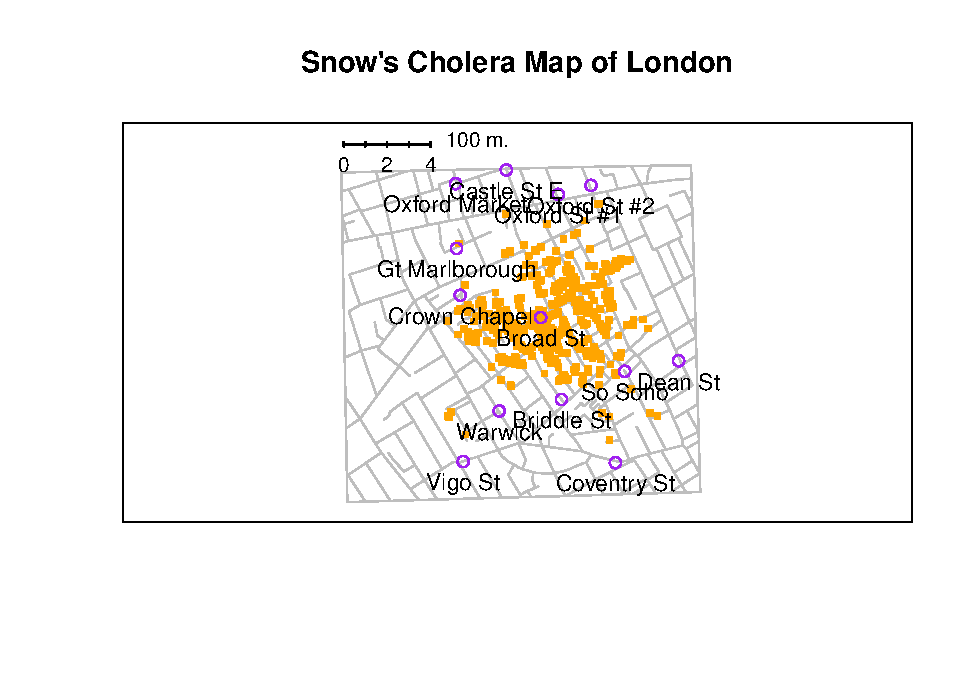
\includegraphics{schuster-statistics-remix_files/figure-latex/snowmap1-1.pdf}
\caption{\label{fig:snowmap1}A stylised redrawing of John Snow's original cholera map. Each small dot represents the location of a cholera case, and each large circle shows the location of a well. As the plot makes clear, the cholera outbreak is centred very closely on the Broad St pump. This image uses the data from the \texttt{HistData} package, and was drawn using minor alterations to the commands provided in the help files. Note that Snow's original hand drawn map used different symbols and labels, but you get the idea.}
\end{figure}

To give a sense of the importance of this chapter, I want to start with a classic illustration of just how powerful a good graph can be. To that end, Figure \ref{fig:snowmap1} shows a redrawing of one of the most famous data visualisations of all time: John Snow's 1854 map of cholera deaths. The map is elegant in its simplicity. In the background we have a street map, which helps orient the viewer. Over the top, we see a large number of small dots, each one representing the location of a cholera case. The larger symbols show the location of water pumps, labelled by name. Even the most casual inspection of the graph makes it very clear that the source of the outbreak is almost certainly the Broad Street pump. Upon viewing this graph, Dr Snow arranged to have the handle removed from the pump, ending the outbreak that had killed over 500 people. Such is the power of a good data visualisation.

The goals in this chapter are twofold: firstly, to discuss several fairly standard graphs that we use a lot when analysing and presenting data, and secondly, to show you how to create these graphs in R. The graphs themselves tend to be pretty straightforward, so in that respect this chapter is pretty simple. Where people usually struggle is learning how to produce graphs, and especially, learning how to produce good graphs.\footnote{I should add that this isn't unique to R. Like everything in R there's a pretty steep learning curve to learning how to draw graphs, and like always there's a massive payoff at the end in terms of the quality of what you can produce. But to be honest, I've seen the same problems show up regardless of what system people use. I suspect that the hardest thing to do is to force yourself to take the time to think deeply about what your graphs are doing. I say that in full knowledge that only about half of my graphs turn out as well as they ought to. Understanding what makes a good graph is easy: actually designing a good graph is \emph{hard}.} Fortunately, learning how to draw graphs in R is reasonably simple, as long as you're not too picky about what your graph looks like. What I mean when I say this is that R has a lot of \emph{very} good graphing functions, and most of the time you can produce a clean, high-quality graphic without having to learn very much about the low-level details of how R handles graphics. Unfortunately, on those occasions when you do want to do something non-standard, or if you need to make highly specific changes to the figure, you actually do need to learn a fair bit about the these details; and those details are both complicated and boring. With that in mind, the structure of this chapter is as follows: I'll start out by giving you a very quick overview of how graphics work in R. I'll then discuss several different kinds of graph and how to draw them, as well as showing the basics of how to customise these plots.

\textbf{Dave note}: \citet{Navarro2018} included a fair amount of under-the-hood detail about how graphs are drawn in R. We do not need that level of theory for now. Instead, I'm including just the least you need to quickly visualize your data.

\hypertarget{introplotting}{%
\subsection{An introduction to plotting}\label{introplotting}}

Before I discuss any specialised graphics, let's start by drawing a few very simple graphs just to get a feel for what it's like to draw pictures using R. To that end, let's create a small vector \texttt{Fibonacci} that contains a few numbers we'd like R to draw for us. Then, we'll ask R to \texttt{plot()} those numbers. The result is Figure \ref{fig:firstplot}.

\begin{Shaded}
\begin{Highlighting}[]
\NormalTok{Fibonacci }\OtherTok{\textless{}{-}} \FunctionTok{c}\NormalTok{( }\DecValTok{1}\NormalTok{,}\DecValTok{1}\NormalTok{,}\DecValTok{2}\NormalTok{,}\DecValTok{3}\NormalTok{,}\DecValTok{5}\NormalTok{,}\DecValTok{8}\NormalTok{,}\DecValTok{13}\NormalTok{ )}
\FunctionTok{plot}\NormalTok{( Fibonacci )}
\end{Highlighting}
\end{Shaded}

\begin{figure}
\centering
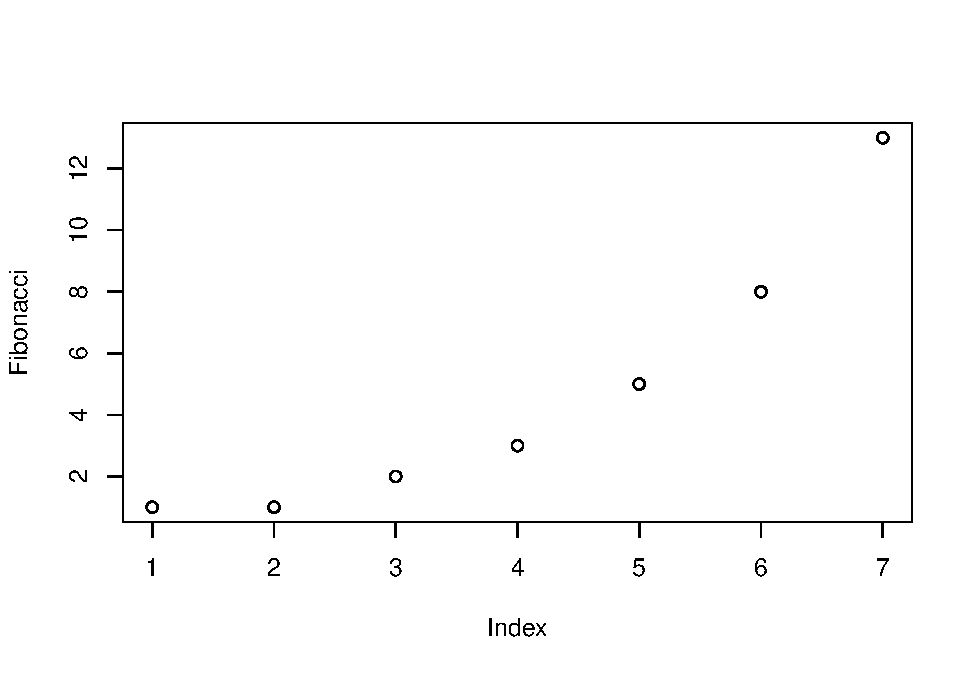
\includegraphics{schuster-statistics-remix_files/figure-latex/firstplot-1.pdf}
\caption{\label{fig:firstplot}Our first plot}
\end{figure}

As you can see, what R has done is plot the \emph{values} stored in the \texttt{Fibonacci} variable on the vertical axis (y-axis) and the corresponding \emph{index} on the horizontal axis (x-axis). In other words, since the 4th element of the vector has a value of 3, we get a dot plotted at the location (4,3). That's pretty straightforward, and the image in Figure \ref{fig:firstplot} is probably pretty close to what you would have had in mind when I suggested that we plot the \texttt{Fibonacci} data.

\hypertarget{figtitles}{%
\subsubsection{Customising the title and the axis labels}\label{figtitles}}

One of the first things that you'll find yourself wanting to do when customising your plot is to label it better. You might want to specify more appropriate axis labels, add a title or add a subtitle. The arguments that you need to specify to make this happen are:

\begin{itemize}
\tightlist
\item
  \texttt{main}. A character string containing the title.
\item
  \texttt{sub}. A character string containing the subtitle.
\item
  \texttt{xlab}. A character string containing the x-axis label.
\item
  \texttt{ylab}. A character string containing the y-axis label.
\end{itemize}

These aren't graphical parameters, they're arguments to the high-level function. However, because the high-level functions all rely on the same low-level function to do the drawing\footnote{The low-level function that does this is called \texttt{title()} in case you ever need to know, and you can type \texttt{?title} to find out a bit more detail about what these arguments do.} the names of these arguments are identical for pretty much every high-level function I've come across. Let's have a look at what happens when we make use of all these arguments. Here's the command. The picture that this draws is shown in Figure \ref{fig:secondplot}.

\begin{Shaded}
\begin{Highlighting}[]
\FunctionTok{plot}\NormalTok{( }\AttributeTok{x =}\NormalTok{ Fibonacci,}
               \AttributeTok{main =} \StringTok{"You specify title using the \textquotesingle{}main\textquotesingle{} argument"}\NormalTok{,}
               \AttributeTok{sub =} \StringTok{"The subtitle appears here! (Use the \textquotesingle{}sub\textquotesingle{} argument for this)"}\NormalTok{,}
               \AttributeTok{xlab =} \StringTok{"The x{-}axis label is \textquotesingle{}xlab\textquotesingle{}"}\NormalTok{,}
                \AttributeTok{ylab =} \StringTok{"The y{-}axis label is \textquotesingle{}ylab\textquotesingle{}"} 
\NormalTok{            )}
\end{Highlighting}
\end{Shaded}

\begin{figure}
\centering
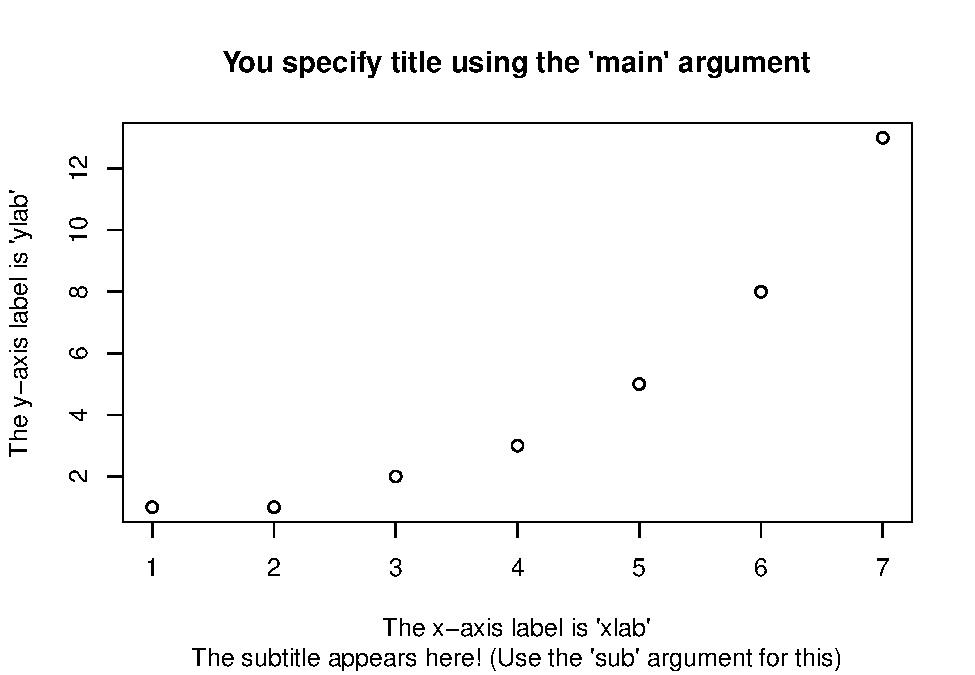
\includegraphics{schuster-statistics-remix_files/figure-latex/secondplot-1.pdf}
\caption{\label{fig:secondplot}How to add your own title, subtitle, x-axis label and y-axis label to the plot.}
\end{figure}

It's more or less as you'd expect. The plot itself is identical to the one we drew in Figure \ref{fig:firstplot}, except for the fact that we've changed the axis labels, and added a title and a subtitle. Even so, there's a couple of interesting features worth calling your attention to. Firstly, notice that the subtitle is drawn below the plot, which I personally find annoying; as a consequence I almost never use subtitles. You may have a different opinion, of course, but the important thing is that you remember where the subtitle actually goes. Secondly, notice that R has decided to use boldface text and a larger font size for the title. This is one of my most hated default settings in R graphics, since I feel that it draws too much attention to the title. Generally, while I do want my reader to look at the title, I find that the R defaults are a bit overpowering, so I often like to change the settings. To that end, there are a bunch of graphical parameters that you can use to customise the font style:

\begin{itemize}
\tightlist
\item
  \emph{Font styles:} \texttt{font.main}, \texttt{font.sub}, \texttt{font.lab}, \texttt{font.axis}. These four parameters control the font style used for the plot title (\texttt{font.main}), the subtitle (\texttt{font.sub}), the axis labels (\texttt{font.lab}: note that you can't specify separate styles for the x-axis and y-axis without using low level commands), and the numbers next to the tick marks on the axis (\texttt{font.axis}). Somewhat irritatingly, these arguments are numbers instead of meaningful names: a value of 1 corresponds to plain text, 2 means boldface, 3 means italic and 4 means bold italic.
\item
  \emph{Font colours:} \texttt{col.main}, \texttt{col.sub}, \texttt{col.lab}, \texttt{col.axis}. These parameters do pretty much what the name says: each one specifies a \textbf{col}our in which to type each of the different bits of text. Conveniently, R has a very large number of named colours (type \texttt{colours()} to see a list of over 650 colour names that R knows), so you can use the English language name of the colour to select it.\footnote{On the off chance that this isn't enough freedom for you, you can select a colour directly as a ``red, green, blue'' specification using the \texttt{rgb()} function, or as a ``hue, saturation, value'' specification using the \texttt{hsv()} function.} Thus, the parameter value here string like \texttt{"red"}, \texttt{"gray25"} or \texttt{"springgreen4"} (yes, R really does recognise four different shades of ``spring green'').
\item
  \emph{Font size:} \texttt{cex.main}, \texttt{cex.sub}, \texttt{cex.lab}, \texttt{cex.axis}. Font size is handled in a slightly curious way in R. The ``cex'' part here is short for ``\textbf{c}haracter \textbf{ex}pansion'', and it's essentially a magnification value. By default, all of these are set to a value of 1, except for the font title: \texttt{cex.main} has a default magnification of 1.2, which is why the title font is 20\% bigger than the others.
\item
  \emph{Font family:} \texttt{family}. This argument specifies a font family to use: the simplest way to use it is to set it to \texttt{"sans"}, \texttt{"serif"}, or \texttt{"mono"}, corresponding to a san serif font, a serif font, or a monospaced font. If you want to, you can give the name of a specific font, but keep in mind that different operating systems use different fonts, so it's probably safest to keep it simple. Better yet, unless you have some deep objections to the R defaults, just ignore this parameter entirely. That's what I usually do.
\end{itemize}

To give you a sense of how you can use these parameters to customise your titles, the following command can be used to draw Figure \ref{fig:thirdplot}:

\begin{Shaded}
\begin{Highlighting}[]
\FunctionTok{plot}\NormalTok{( }\AttributeTok{x =}\NormalTok{ Fibonacci,                           }\CommentTok{\# the data to plot}
          \AttributeTok{main =} \StringTok{"The first 7 Fibonacci numbers"}\NormalTok{,  }\CommentTok{\# the title}
          \AttributeTok{xlab =} \StringTok{"Position in the sequence"}\NormalTok{,       }\CommentTok{\# x{-}axis label}
          \AttributeTok{ylab =} \StringTok{"The Fibonacci number"}\NormalTok{,           }\CommentTok{\# y{-}axis }
          \AttributeTok{font.main =} \DecValTok{1}\NormalTok{,}
          \AttributeTok{cex.main =} \DecValTok{1}\NormalTok{,}
          \AttributeTok{font.axis =} \DecValTok{2}\NormalTok{,}
          \AttributeTok{col.lab =} \StringTok{"gray50"}\NormalTok{ )}
\end{Highlighting}
\end{Shaded}

\begin{figure}
\centering
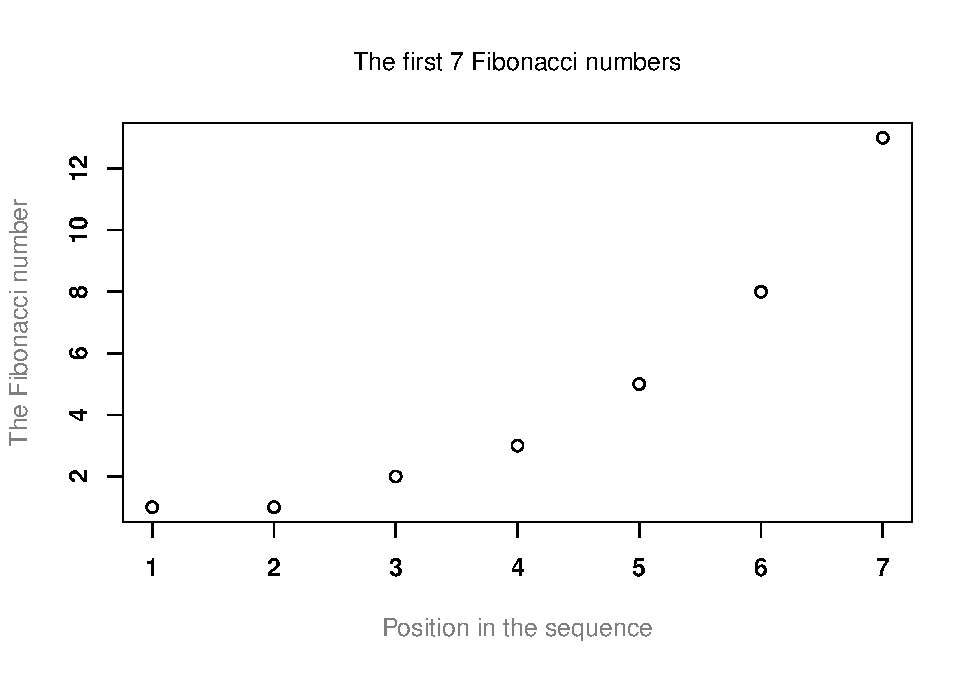
\includegraphics{schuster-statistics-remix_files/figure-latex/thirdplot-1.pdf}
\caption{\label{fig:thirdplot}How to customise the appearance of the titles and labels.}
\end{figure}

Although this command is quite long, it's not complicated: all it does is override a bunch of the default parameter values. The only difficult aspect to this is that you have to remember what each of these parameters is called, and what all the different values are. And in practice I never remember: I have to look up the help documentation every time, or else look it up in this book.

\hypertarget{hist}{%
\subsection{Histograms}\label{hist}}

Now that we've tamed (or possibly fled from) the beast that is R graphical parameters, let's talk more seriously about some real life graphics that you'll want to draw. We begin with the humble \textbf{\emph{histogram}}. Histograms are one of the simplest and most useful ways of visualising data. They make most sense when you have an interval or ratio scale (e.g., the \texttt{afl.margins} data from Chapter \ref{descriptives} and what you want to do is get an overall impression of the data. Most of you probably know how histograms work, since they're so widely used, but for the sake of completeness I'll describe them. All you do is divide up the possible values into \textbf{\emph{bins}}, and then count the number of observations that fall within each bin. This count is referred to as the frequency of the bin, and is displayed as a bar: in the AFL winning margins data, there are 33 games in which the winning margin was less than 10 points, and it is this fact that is represented by the height of the leftmost bar in Figure \ref{fig:hist1a}. Drawing this histogram in R is pretty straightforward. The function you need to use is called \texttt{hist()}, and it has pretty reasonable default settings. In fact, Figure \ref{fig:hist1a} is exactly what you get if you just type this:

\begin{Shaded}
\begin{Highlighting}[]
\FunctionTok{hist}\NormalTok{( afl.margins )}
\end{Highlighting}
\end{Shaded}

\begin{figure}
\centering
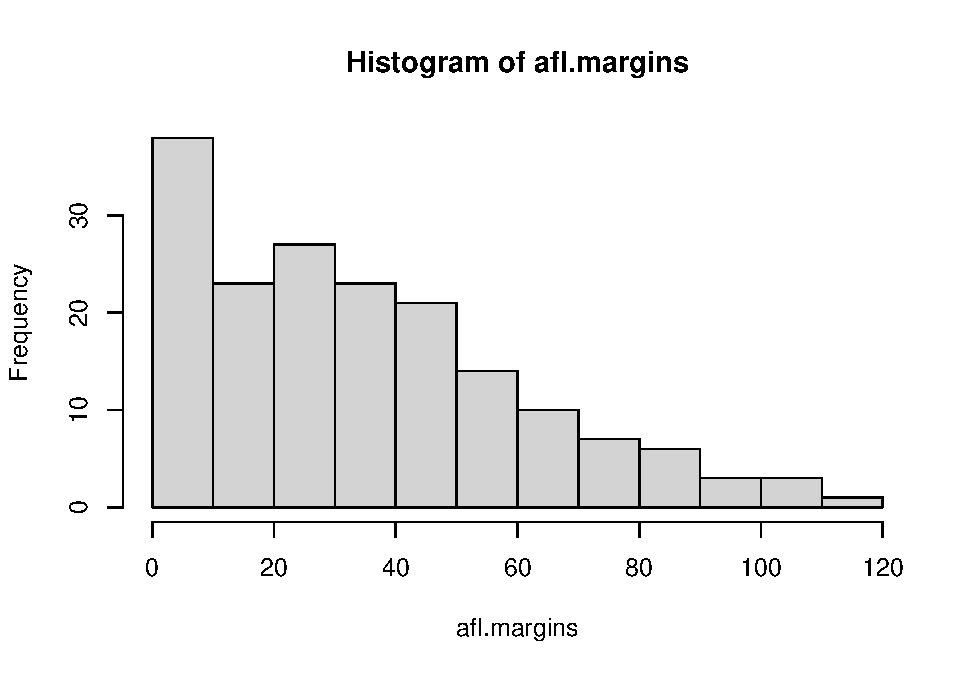
\includegraphics{schuster-statistics-remix_files/figure-latex/hist1a-1.pdf}
\caption{\label{fig:hist1a}The default histogram that R produces}
\end{figure}

Although this image would need a lot of cleaning up in order to make a good presentation graphic (i.e., one you'd include in a report), it nevertheless does a pretty good job of describing the data. In fact, the big strength of a histogram is that (properly used) it does show the entire spread of the data, so you can get a pretty good sense about what it looks like. The downside to histograms is that they aren't very compact: unlike some of the other plots I'll talk about it's hard to cram 20-30 histograms into a single image without overwhelming the viewer. And of course, if your data are nominal scale (e.g., the \texttt{afl.finalists} data) then histograms are useless.

The main subtlety that you need to be aware of when drawing histograms is determining where the \texttt{breaks} that separate bins should be located, and (relatedly) how many breaks there should be. In Figure \ref{fig:hist1a}, you can see that R has made pretty sensible choices all by itself: the breaks are located at 0, 10, 20, \ldots{} 120, which is exactly what I would have done had I been forced to make a choice myself. On the other hand, consider the two histograms in Figure \ref{fig:hist1b} and \ref{fig:hist1c}, which I produced using the following two commands:

\begin{Shaded}
\begin{Highlighting}[]
\FunctionTok{hist}\NormalTok{( }\AttributeTok{x =}\NormalTok{ afl.margins, }\AttributeTok{breaks =} \DecValTok{3}\NormalTok{ )}
\end{Highlighting}
\end{Shaded}

\begin{figure}
\centering
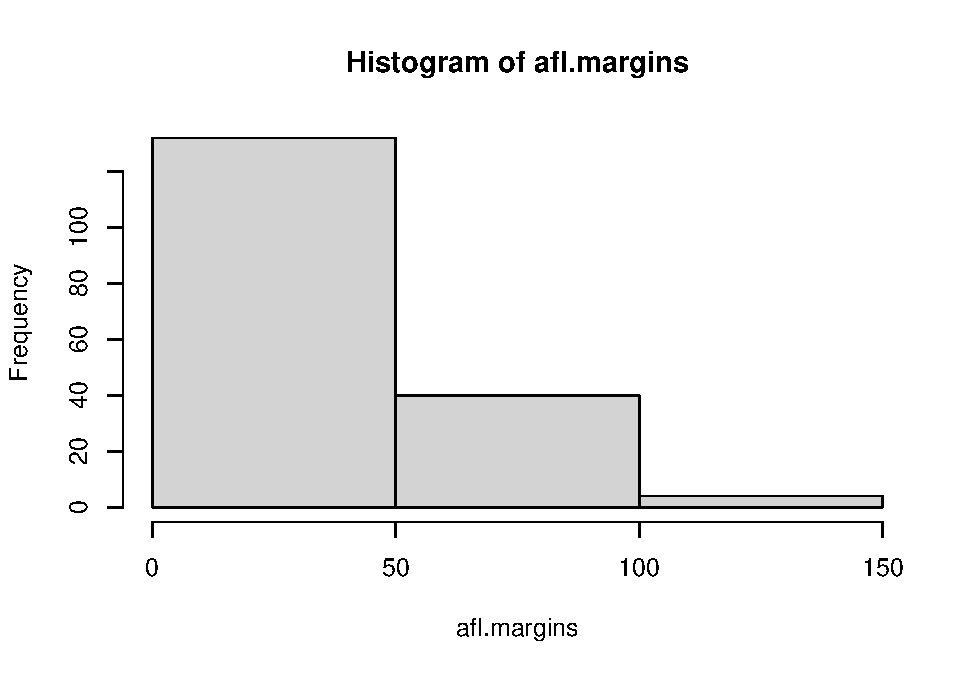
\includegraphics{schuster-statistics-remix_files/figure-latex/hist1b-1.pdf}
\caption{\label{fig:hist1b}A histogram with too few bins}
\end{figure}

\begin{Shaded}
\begin{Highlighting}[]
\FunctionTok{hist}\NormalTok{( }\AttributeTok{x =}\NormalTok{ afl.margins, }\AttributeTok{breaks =} \DecValTok{0}\SpecialCharTok{:}\DecValTok{116}\NormalTok{ )}
\end{Highlighting}
\end{Shaded}

\begin{figure}
\centering
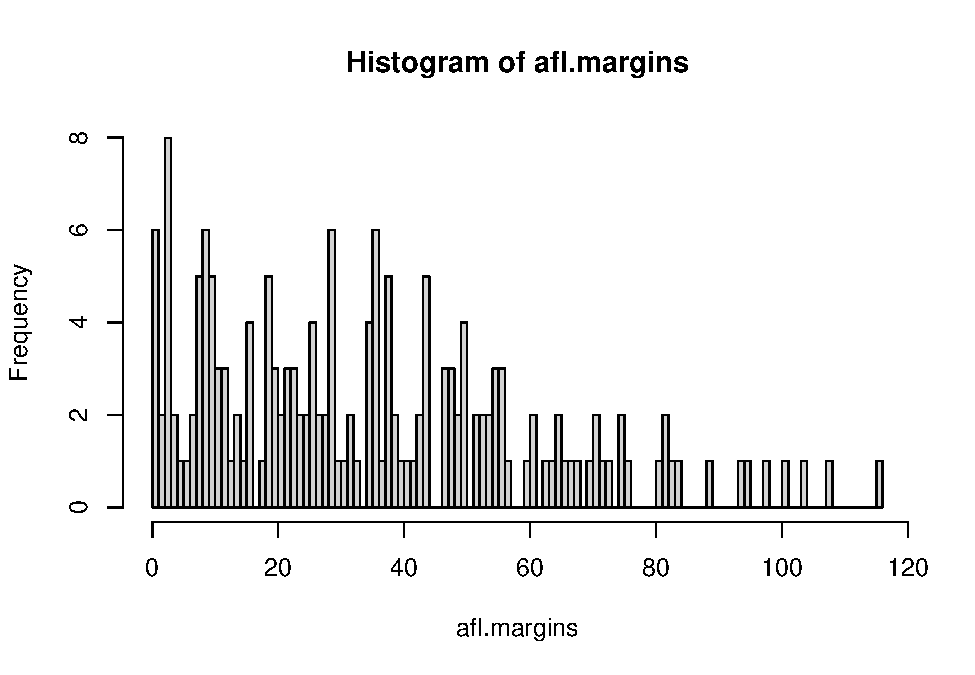
\includegraphics{schuster-statistics-remix_files/figure-latex/hist1c-1.pdf}
\caption{\label{fig:hist1c}A histogram with too many bins}
\end{figure}

In Figure \ref{fig:hist1c}, the bins are only 1 point wide. As a result, although the plot is very informative (it displays the entire data set with no loss of information at all!) the plot is very hard to interpret, and feels quite cluttered. On the other hand, the plot in Figure \ref{fig:hist1b} has a bin width of 50 points, and has the opposite problem: it's very easy to ``read'' this plot, but it doesn't convey a lot of information. One gets the sense that this histogram is hiding too much. In short, the way in which you specify the breaks has a big effect on what the histogram looks like, so it's important to make sure you choose the breaks sensibly. In general R does a pretty good job of selecting the breaks on its own, since it makes use of some quite clever tricks that statisticians have devised for automatically selecting the right bins for a histogram, but nevertheless it's usually a good idea to play around with the breaks a bit to see what happens.

There is one fairly important thing to add regarding how the \texttt{breaks} argument works. There are two different ways you can specify the breaks. You can either specify \emph{how many} breaks you want (which is what I did for panel b when I typed \texttt{breaks\ =\ 3}) and let R figure out where they should go, or you can provide a vector that tells R exactly where the breaks should be placed (which is what I did for panel c when I typed \texttt{breaks\ =\ 0:116}). The behaviour of the \texttt{hist()} function is slightly different depending on which version you use. If all you do is tell it \emph{how many} breaks you want, R treats it as a ``suggestion'' not as a demand. It assumes you want ``approximately 3'' breaks, but if it doesn't think that this would look very pretty on screen, it picks a different (but similar) number. It does this for a sensible reason -- it tries to make sure that the breaks are located at sensible values (like 10) rather than stupid ones (like 7.224414). And most of the time R is right: usually, when a human researcher says ``give me 3 breaks'', he or she really does mean ``give me approximately 3 breaks, and don't put them in stupid places''. However, sometimes R is dead wrong. Sometimes you really do mean ``exactly 3 breaks'', and you know precisely where you want them to go. So you need to invoke ``real person privilege'', and order R to do what it's bloody well told. In order to do that, you \emph{have} to input the full vector that tells R exactly where you want the breaks. If you do that, R will go back to behaving like the nice little obedient calculator that it's supposed to be.

\hypertarget{visual-style-of-your-histogram}{%
\subsubsection{Visual style of your histogram}\label{visual-style-of-your-histogram}}

Okay, so at this point we can draw a basic histogram, and we can alter the number and even the location of the \texttt{breaks}. However, the visual style of the histograms shown in Figures \ref{fig:hist1a}, \ref{fig:hist1b}, and \ref{fig:hist1c} could stand to be improved. We can fix this by making use of some of the other arguments to the \texttt{hist()} function. Most of the things you might want to try doing have already been covered in Section \ref{introplotting}, but there's a few new things:

\begin{itemize}
\tightlist
\item
  \emph{Shading lines}: \texttt{density}, \texttt{angle}. You can add diagonal lines to shade the bars: the \texttt{density} value is a number indicating how many lines per inch R should draw (the default value of \texttt{NULL} means no lines), and the \texttt{angle} is a number indicating how many degrees from horizontal the lines should be drawn at (default is \texttt{angle\ =\ 45} degrees).
\item
  \emph{Specifics regarding colours}: \texttt{col}, \texttt{border}. You can also change the colours: in this instance the \texttt{col} parameter sets the colour of the shading (either the shading lines if there are any, or else the colour of the interior of the bars if there are not), and the \texttt{border} argument sets the colour of the edges of the bars.
\item
  \emph{Labelling the bars}: \texttt{labels}. You can also attach labels to each of the bars using the \texttt{labels} argument. The simplest way to do this is to set \texttt{labels\ =\ TRUE}, in which case R will add a number just above each bar, that number being the exact number of observations in the bin. Alternatively, you can choose the labels yourself, by inputting a vector of strings, e.g., \texttt{labels\ =\ c("label\ 1","label\ 2","etc")}
\end{itemize}

Not surprisingly, this doesn't exhaust the possibilities. If you type \texttt{help("hist")} or \texttt{?hist} and have a look at the help documentation for histograms, you'll see a few more options. A histogram that makes use of the histogram-specific customisations as well as several of the options we discussed in Section \ref{introplotting} is shown in Figure \ref{fig:hist1d}. The R command that I used to draw it is this:

\begin{Shaded}
\begin{Highlighting}[]
\FunctionTok{hist}\NormalTok{( }\AttributeTok{x =}\NormalTok{ afl.margins, }
      \AttributeTok{main =} \StringTok{"2010 AFL margins"}\NormalTok{, }\CommentTok{\# title of the plot}
      \AttributeTok{xlab =} \StringTok{"Margin"}\NormalTok{,           }\CommentTok{\# set the x{-}axis label}
      \AttributeTok{density =} \DecValTok{10}\NormalTok{,              }\CommentTok{\# draw shading lines: 10 per inch}
      \AttributeTok{angle =} \DecValTok{40}\NormalTok{,                }\CommentTok{\# set the angle of the shading lines is 40 degrees}
      \AttributeTok{border =} \StringTok{"gray20"}\NormalTok{,         }\CommentTok{\# set the colour of the borders of the bars}
      \AttributeTok{col =} \StringTok{"gray80"}\NormalTok{,            }\CommentTok{\# set the colour of the shading lines}
      \AttributeTok{labels =} \ConstantTok{TRUE}\NormalTok{,             }\CommentTok{\# add frequency labels to each bar}
      \AttributeTok{ylim =} \FunctionTok{c}\NormalTok{(}\DecValTok{0}\NormalTok{,}\DecValTok{40}\NormalTok{)             }\CommentTok{\# change the scale of the y{-}axis}
\NormalTok{)}
\end{Highlighting}
\end{Shaded}

\begin{figure}
\centering
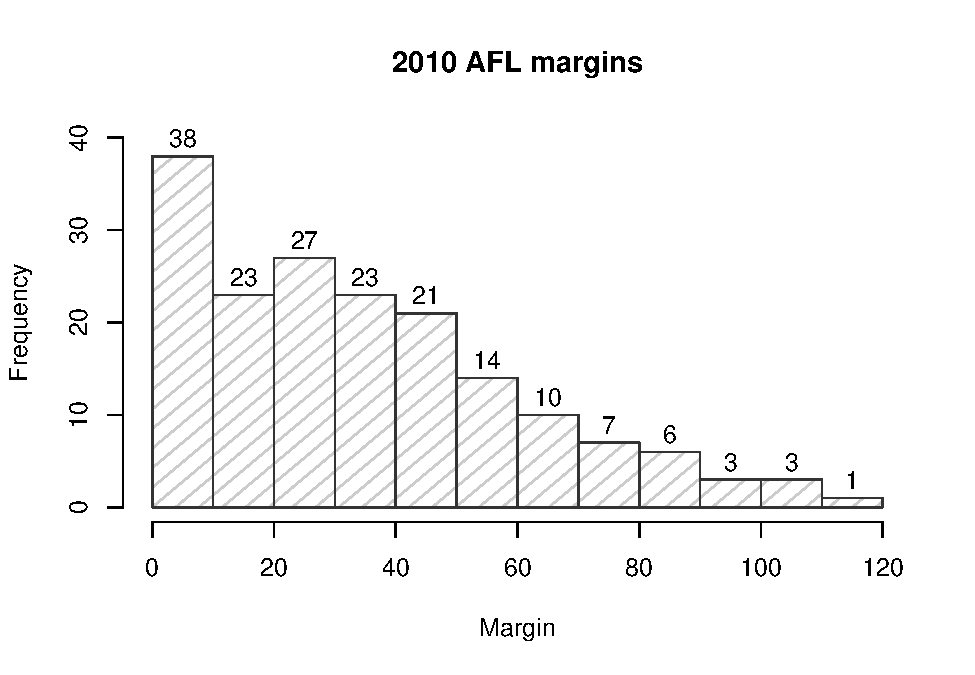
\includegraphics{schuster-statistics-remix_files/figure-latex/hist1d-1.pdf}
\caption{\label{fig:hist1d}A histogram with histogram specific customisations}
\end{figure}

Overall, this is a much nicer histogram than the default ones.

\hypertarget{boxplots}{%
\subsection{Boxplots}\label{boxplots}}

Another alternative to histograms is a \textbf{\emph{boxplot}}, sometimes called a ``box and whiskers'' plot. Like histograms, they're most suited to interval or ratio scale data. The idea behind a boxplot is to provide a simple visual depiction of the median, the interquartile range, and the range of the data. And because they do so in a fairly compact way, boxplots have become a very popular statistical graphic, especially during the exploratory stage of data analysis when you're trying to understand the data yourself. Let's have a look at how they work, again using the \texttt{afl.margins} data as our example. Firstly, let's actually calculate these numbers ourselves using the \texttt{summary()} function:\footnote{R being what it is, it's no great surprise that there's also a \texttt{fivenum()} function that does much the same thing.}

\begin{Shaded}
\begin{Highlighting}[]
\FunctionTok{summary}\NormalTok{( afl.margins )}
\end{Highlighting}
\end{Shaded}

\begin{verbatim}
##    Min. 1st Qu.  Median    Mean 3rd Qu.    Max. 
##    0.00   12.75   30.50   35.30   50.50  116.00
\end{verbatim}

So how does a boxplot capture these numbers? The easiest way to describe what a boxplot looks like is just to draw one. The function for doing this in R is (surprise, surprise) \texttt{boxplot()}. As always there's a lot of optional arguments that you can specify if you want, but for the most part you can just let R choose the defaults for you. That said, I'm going to override one of the defaults to start with by specifying the \texttt{range} option, but for the most part you won't want to do this (I'll explain why in a minute). With that as preamble, let's try the following command:

\begin{Shaded}
\begin{Highlighting}[]
\FunctionTok{boxplot}\NormalTok{( }\AttributeTok{x =}\NormalTok{ afl.margins, }\AttributeTok{range =} \DecValTok{100}\NormalTok{ )}
\end{Highlighting}
\end{Shaded}

\begin{figure}
\centering
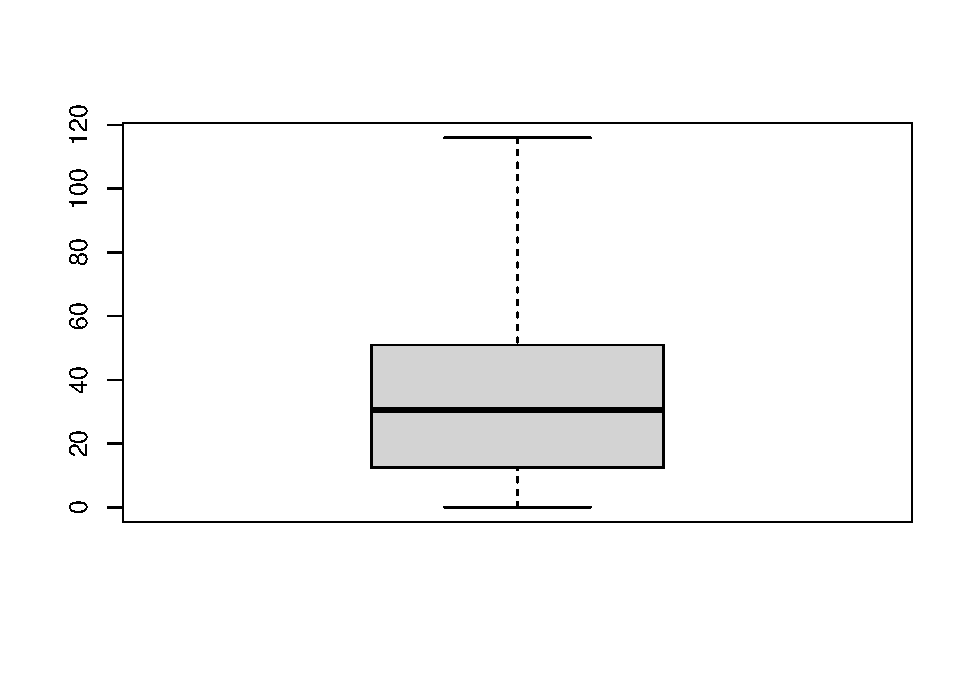
\includegraphics{schuster-statistics-remix_files/figure-latex/boxplot1a-1.pdf}
\caption{\label{fig:boxplot1a}A basic boxplot}
\end{figure}

What R draws is shown in Figure \ref{fig:boxplot1a}, the most basic boxplot possible. When you look at this plot, this is how you should interpret it: the thick line in the middle of the box is the median; the box itself spans the range from the 25th percentile to the 75th percentile; and the ``whiskers'' cover the full range from the minimum value to the maximum value. This is summarised in the annotated plot in Figure \ref{fig:boxplot1b}.

\begin{figure}
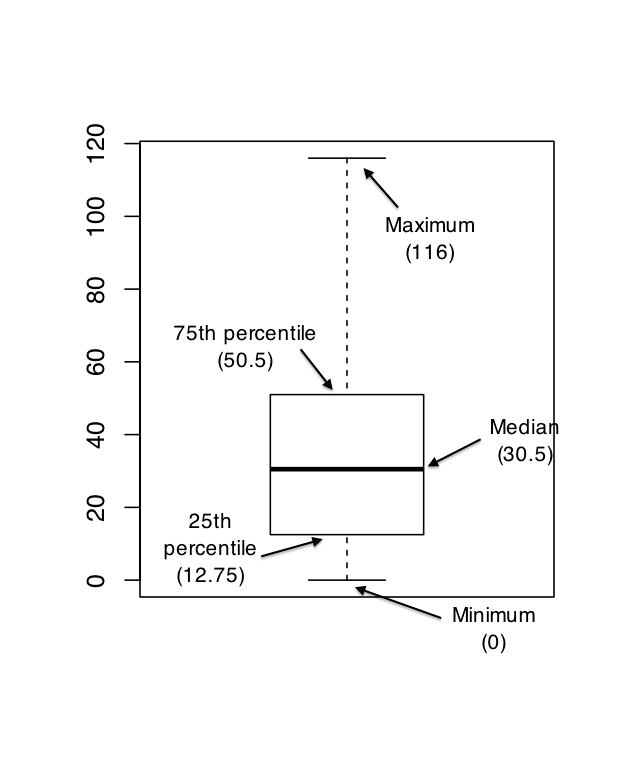
\includegraphics[width=8.33in]{/Users/dave/Documents/GitHub/stats-remix-advanced/bookdown/img/graphics2/boxplot1_annotated} \caption{An annotated boxplot}\label{fig:boxplot1b}
\end{figure}

In practice, this isn't quite how boxplots usually work. In most applications, the ``whiskers'' don't cover the full range from minimum to maximum. Instead, they actually go out to the most extreme data point that doesn't exceed a certain bound. By default, this value is 1.5 times the interquartile range, corresponding to a \texttt{range} value of 1.5. Any observation whose value falls outside this range is plotted as a circle instead of being covered by the whiskers, and is commonly referred to as an \textbf{\emph{outlier}}. For our AFL margins data, there is one observation (a game with a margin of 116 points) that falls outside this range. As a consequence, the upper whisker is pulled back to the next largest observation (a value of 108), and the observation at 116 is plotted as a circle. This is illustrated in Figure \ref{fig:boxplot2a}. Since the default value is \texttt{range\ =\ 1.5} we can draw this plot using the simple command

\begin{Shaded}
\begin{Highlighting}[]
\FunctionTok{boxplot}\NormalTok{( afl.margins )}
\end{Highlighting}
\end{Shaded}

\begin{figure}
\centering
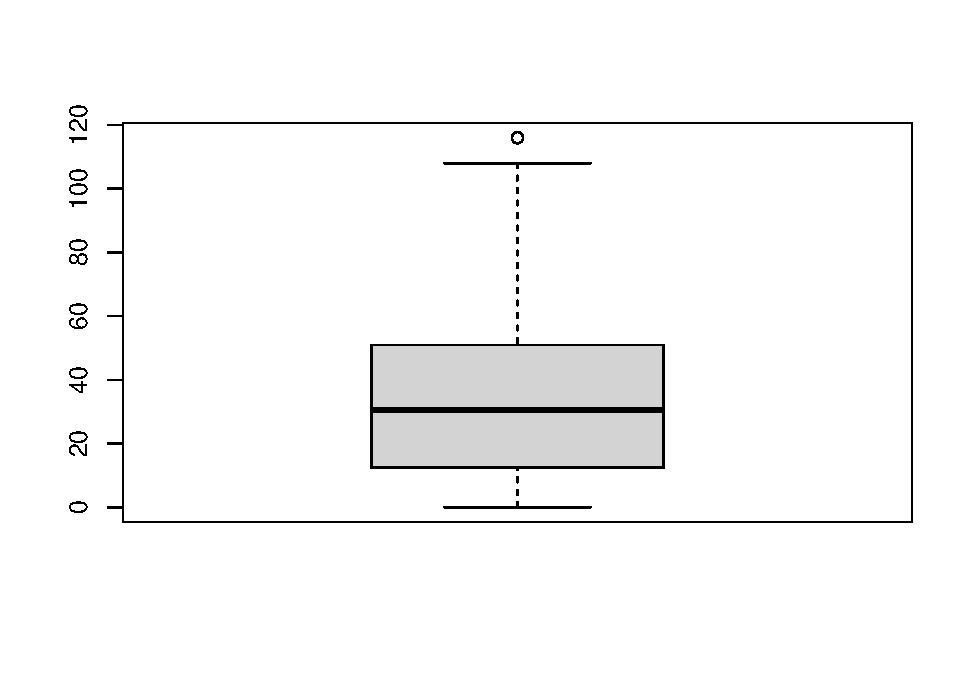
\includegraphics{schuster-statistics-remix_files/figure-latex/boxplot2a-1.pdf}
\caption{\label{fig:boxplot2a}By default, R will only extent the whiskers a distance of 1.5 times the interquartile range, and will plot any points that fall outside that range separately}
\end{figure}

\hypertarget{visual-style-of-your-boxplot}{%
\subsubsection{Visual style of your boxplot}\label{visual-style-of-your-boxplot}}

I'll talk a little more about the relationship between boxplots and outliers in the Section \ref{boxplotoutliers}, but before I do let's take the time to clean this figure up. Boxplots in R are extremely customisable. In addition to the usual range of graphical parameters that you can tweak to make the plot look nice, you can also exercise nearly complete control over every element to the plot. Consider the boxplot in Figure \ref{fig:boxplot2b}: in this version of the plot, not only have I added labels (\texttt{xlab}, \texttt{ylab}) and removed the stupid border (\texttt{frame.plot}), I've also dimmed all of the graphical elements of the boxplot except the central bar that plots the median (\texttt{border}) so as to draw more attention to the median rather than the rest of the boxplot.

\begin{figure}
\centering
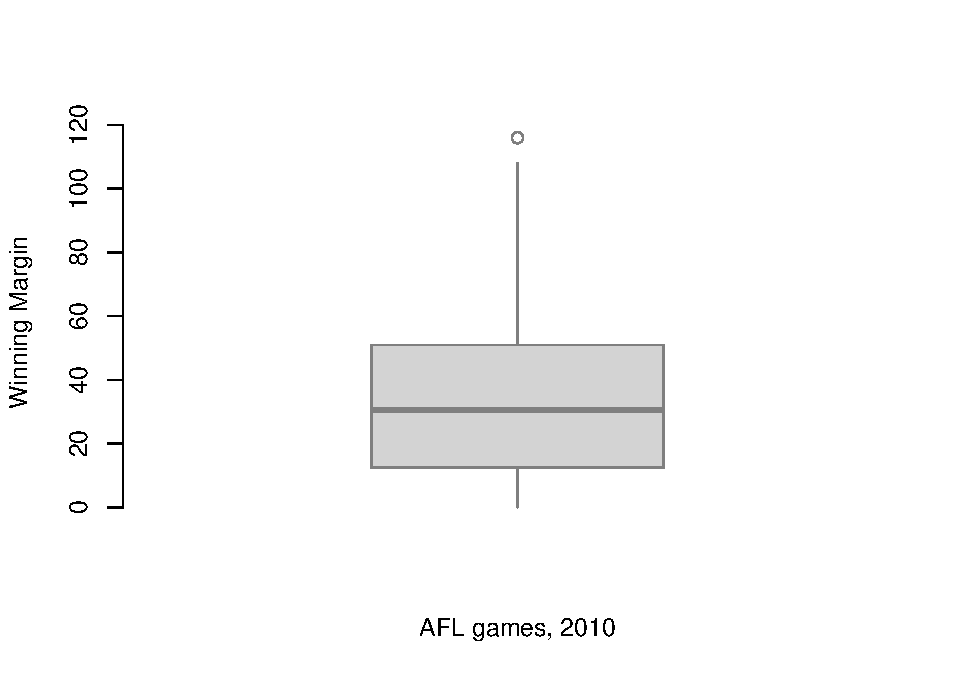
\includegraphics{schuster-statistics-remix_files/figure-latex/boxplot2b-1.pdf}
\caption{\label{fig:boxplot2b}A boxplot with boxplot specific customisations}
\end{figure}

You've seen all these options in previous sections in this chapter, so hopefully those customisations won't need any further explanation. However, I've done two new things as well: I've deleted the cross-bars at the top and bottom of the whiskers (known as the ``staples'' of the plot), and converted the whiskers themselves to solid lines. The arguments that I used to do this are called by the ridiculous names of \texttt{staplewex} and \texttt{whisklty},\footnote{I realise there's a kind of logic to the way R names are constructed, but they still sound dumb. When I typed this sentence, all I could think was that it sounded like the name of a kids movie if it had been written by Lewis Carroll: ``The frabjous gambolles of Staplewex and Whisklty'' or something along those lines.} and I'll explain these in a moment.

But first, here's the actual command I used to draw this figure:

\begin{Shaded}
\begin{Highlighting}[]
\FunctionTok{boxplot}\NormalTok{( }\AttributeTok{x =}\NormalTok{ afl.margins,           }\CommentTok{\# the data}
          \AttributeTok{xlab =} \StringTok{"AFL games, 2010"}\NormalTok{,  }\CommentTok{\# x{-}axis label}
          \AttributeTok{ylab =} \StringTok{"Winning Margin"}\NormalTok{,   }\CommentTok{\# y{-}axis label}
          \AttributeTok{border =} \StringTok{"grey50"}\NormalTok{,         }\CommentTok{\# dim the border of the box}
          \AttributeTok{frame.plot =} \ConstantTok{FALSE}\NormalTok{,        }\CommentTok{\# don\textquotesingle{}t draw a frame}
          \AttributeTok{staplewex =} \DecValTok{0}\NormalTok{,             }\CommentTok{\# don\textquotesingle{}t draw staples}
          \AttributeTok{whisklty =} \DecValTok{1}               \CommentTok{\# solid line for whisker }
\NormalTok{ )}
\end{Highlighting}
\end{Shaded}

Overall, I think the resulting boxplot is a huge improvement in visual design over the default version. In my opinion at least, there's a fairly minimalist aesthetic that governs good statistical graphics. Ideally, every visual element that you add to a plot should convey part of the message. If your plot includes things that don't actually help the reader learn anything new, you should consider removing them. Personally, I can't see the point of the cross-bars on a standard boxplot, so I've deleted them.

\hypertarget{boxplotoutliers}{%
\subsubsection{Using box plots to detect outliers}\label{boxplotoutliers}}

Because the boxplot automatically (unless you change the \texttt{range} argument) separates out those observations that lie within a certain range, people often use them as an informal method for detecting \textbf{\emph{outliers}}: observations that are ``suspiciously'' distant from the rest of the data. Here's an example. Suppose that I'd drawn the boxplot for the AFL margins data, and it came up looking like Figure \ref{fig:boxplotoutlier}.

\begin{figure}
\centering
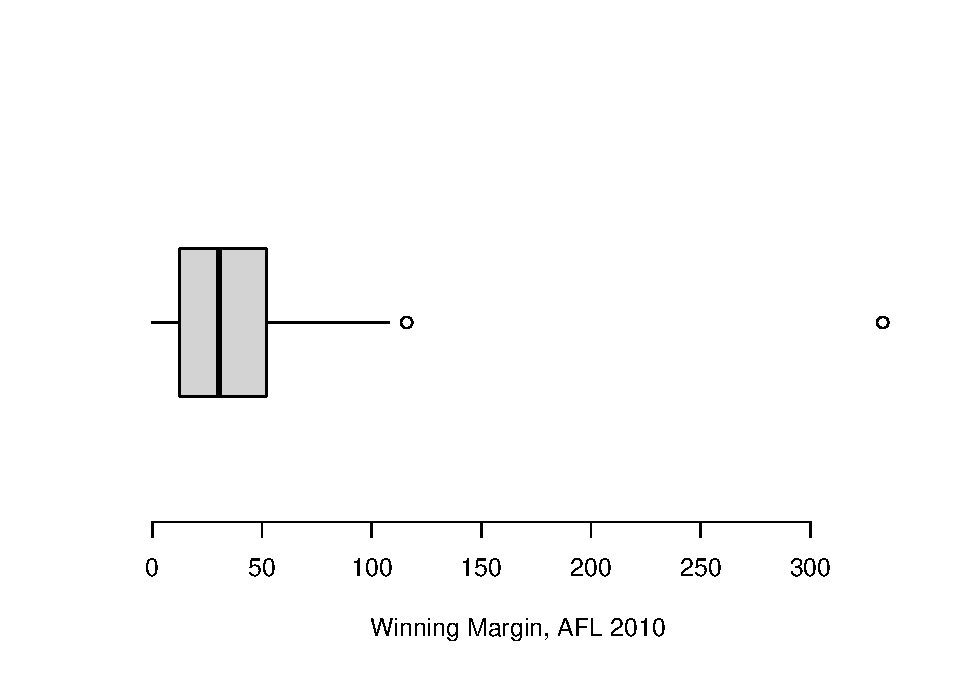
\includegraphics{schuster-statistics-remix_files/figure-latex/boxplotoutlier-1.pdf}
\caption{\label{fig:boxplotoutlier}A boxplot showing one very suspicious outlier! I've drawn this plot in a similar, minimalist style to the one in Figure \ref{fig:boxplot2b}, but I've used the \texttt{horizontal} argument to draw it sideways in order to save space.}
\end{figure}

It's pretty clear that something funny is going on with one of the observations. Apparently, there was one game in which the margin was over 300 points! That doesn't sound right to me. Now that I've become suspicious, it's time to look a bit more closely at the data. One function that can be handy for this is the \texttt{which()} function; it takes as input a vector of logicals, and outputs the indices of the \texttt{TRUE} cases. This is particularly useful in the current context because it lets me do this:

\begin{Shaded}
\begin{Highlighting}[]
\NormalTok{suspicious.cases }\OtherTok{\textless{}{-}}\NormalTok{ afl.margins }\SpecialCharTok{\textgreater{}} \DecValTok{300}
\FunctionTok{which}\NormalTok{( suspicious.cases )}
\end{Highlighting}
\end{Shaded}

\begin{verbatim}
## [1] 137
\end{verbatim}

although in real life I probably wouldn't bother creating the \texttt{suspicious.cases} variable: I'd just cut out the middle man and use a command like \texttt{which(\ afl.margins\ \textgreater{}\ 300\ )}. In any case, what this has done is shown me that the outlier corresponds to game 137. Then, I find the recorded margin for that game:

\begin{Shaded}
\begin{Highlighting}[]
\NormalTok{afl.margins[}\DecValTok{137}\NormalTok{]}
\end{Highlighting}
\end{Shaded}

\begin{verbatim}
## [1] 333
\end{verbatim}

Hm. That definitely doesn't sound right. So then I go back to the original data source (the internet!) and I discover that the actual margin of that game was 33 points. Now it's pretty clear what happened. Someone must have typed in the wrong number. Easily fixed, just by typing \texttt{afl.margins{[}137{]}\ \textless{}-\ 33}. While this might seem like a silly example, I should stress that this kind of thing actually happens a lot. Real world data sets are often riddled with stupid errors, especially when someone had to type something into a computer at some point. In fact, there's actually a name for this phase of data analysis, since in practice it can waste a huge chunk of our time: \textbf{\emph{data cleaning}}. It involves searching for typos, missing data and all sorts of other obnoxious errors in raw data files.\footnote{Sometimes it's convenient to have the boxplot automatically label the outliers for you. The original \texttt{boxplot()} function doesn't allow you to do this; however, the \texttt{Boxplot()} function in the \texttt{car} package does. The design of the \texttt{Boxplot()} function is very similar to \texttt{boxplot()}. It just adds a few new arguments that allow you to tweak the labelling scheme. I'll leave it to the reader to check this out.}

What about the real data? Does the value of 116 constitute a funny observation not? Possibly. As it turns out the game in question was Fremantle v Hawthorn, and was played in round 21 (the second last home and away round of the season). Fremantle had already qualified for the final series and for them the outcome of the game was irrelevant; and the team decided to rest several of their star players. As a consequence, Fremantle went into the game severely underpowered. In contrast, Hawthorn had started the season very poorly but had ended on a massive winning streak, and for them a win could secure a place in the finals. With the game played on Hawthorn's home turf\footnote{Sort of. The game was played in Launceston, which is a de facto home away from home for Hawthorn.} and with so many unusual factors at play, it is perhaps no surprise that Hawthorn annihilated Fremantle by 116 points. Two weeks later, however, the two teams met again in an elimination final on Fremantle's home ground, and Fremantle won comfortably by 30 points.\footnote{Contrast this situation with the next largest winning margin in the data set, which was Geelong's 108 point demolition of Richmond in round 6 at their home ground, Kardinia Park. Geelong have been one of the most dominant teams over the last several years, a period during which they strung together an incredible 29-game winning streak at Kardinia Park. Richmond have been useless for several years. This is in no meaningful sense an outlier. Geelong have been winning by these margins (and Richmond losing by them) for quite some time. Frankly I'm surprised that the result wasn't more lopsided: as happened to Melbourne in 2011 when Geelong won by a modest 186 points.}

So, should we exclude the game from subsequent analyses? If this were a psychology experiment rather than an AFL season, I'd be quite tempted to exclude it because there's pretty strong evidence that Fremantle weren't really trying very hard: and to the extent that my research question is based on an assumption that participants are genuinely trying to do the task. On the other hand, in a lot of studies we're actually interested in seeing the full range of possible behaviour, and that includes situations where people decide not to try very hard: so excluding that observation would be a bad idea. In the context of the AFL data, a similar distinction applies. If I'd been trying to make tips about who would perform well in the finals, I would have (and in fact did) disregard the Round 21 massacre, because it's way too misleading. On the other hand, if my interest is solely in the home and away season itself, I think it would be a shame to throw away information pertaining to one of the most distinctive (if boring) games of the year. In other words, the decision about whether to include outliers or exclude them depends heavily on \emph{why} you think the data look they way they do, and what you want to use the data \emph{for}. Statistical tools can provide an automatic method for suggesting candidates for deletion, but you really need to exercise good judgment here. As I've said before, R is a mindless automaton. It doesn't watch the footy, so it lacks the broader context to make an informed decision. You are \emph{not} a mindless automaton, so you should exercise judgment: if the outlier looks legitimate to you, then keep it. In any case, I'll return to the topic again in Section \ref{regressiondiagnostics}, so let's return to our discussion of how to draw boxplots.

\hypertarget{multipleboxplots}{%
\subsubsection{Drawing multiple boxplots}\label{multipleboxplots}}

One last thing. What if you want to draw multiple boxplots at once? Suppose, for instance, I wanted separate boxplots showing the AFL margins not just for 2010, but for every year between 1987 and 2010. To do that, the first thing we'll have to do is find the data. These are stored in the \texttt{aflsmall2.Rdata} file. So let's load it and take a quick peek at what's inside:

\begin{Shaded}
\begin{Highlighting}[]
\FunctionTok{load}\NormalTok{( }\StringTok{"aflsmall2.Rdata"}\NormalTok{ )}
\FunctionTok{who}\NormalTok{( }\ConstantTok{TRUE}\NormalTok{ )}
\CommentTok{\#   {-}{-} Name {-}{-}   {-}{-} Class {-}{-}   {-}{-} Size {-}{-}}
\CommentTok{\#   afl2         data.frame    4296 x 2  }
\CommentTok{\#    $margin     numeric       4296      }
\CommentTok{\#    $year       numeric       4296     }
\end{Highlighting}
\end{Shaded}

Notice that \texttt{afl2} data frame is pretty big. It contains 4296 games, which is far more than I want to see printed out on my computer screen. To that end, R provides you with a few useful functions to print out only a few of the row in the data frame. The first of these is \texttt{head()} which prints out the first 6 rows, of the data frame, like this:

\begin{Shaded}
\begin{Highlighting}[]
\FunctionTok{head}\NormalTok{( afl2 )}
\end{Highlighting}
\end{Shaded}

\begin{verbatim}
##   margin year
## 1     33 1987
## 2     59 1987
## 3     45 1987
## 4     91 1987
## 5     39 1987
## 6      1 1987
\end{verbatim}

You can also use the \texttt{tail()} function to print out the last 6 rows. The \texttt{car} package also provides a handy little function called \texttt{some()} which prints out a random subset of the rows.

In any case, the important thing is that we have the \texttt{afl2} data frame which contains the variables that we're interested in. What we want to do is have R draw boxplots for the \texttt{margin} variable, plotted separately for each separate \texttt{year}. The way to do this using the \texttt{boxplot()} function is to input a \texttt{formula} rather than a variable as the input. In this case, the formula we want is \texttt{margin\ \textasciitilde{}\ year}. So our boxplot command now looks like this. The result is shown in Figure \ref{fig:multipleboxplots}.\footnote{Actually, there's other ways to do this. If the input argument \texttt{x} is a list object (see Section \ref{lists}, the \texttt{boxplot()} function will draw a separate boxplot for each variable in that list. Relatedly, since the \texttt{plot()} function -- which we'll discuss shortly -- is a generic (see Section \ref{generics}, you might not be surprised to learn that one of its special cases is a boxplot: specifically, if you use \texttt{plot()} where the first argument \texttt{x} is a factor and the second argument \texttt{y} is numeric, then the result will be a boxplot, showing the values in \texttt{y}, with a separate boxplot for each level. For instance, something like \texttt{plot(x\ =\ afl2\textbackslash{}\$year,\ y\ =\ afl2\textbackslash{}\$margin)} would work.}

\begin{Shaded}
\begin{Highlighting}[]
\FunctionTok{boxplot}\NormalTok{( }\AttributeTok{formula =}\NormalTok{ margin }\SpecialCharTok{\textasciitilde{}}\NormalTok{ year,}
         \AttributeTok{data =}\NormalTok{ afl2}
\NormalTok{)}
\end{Highlighting}
\end{Shaded}

\begin{figure}
\centering
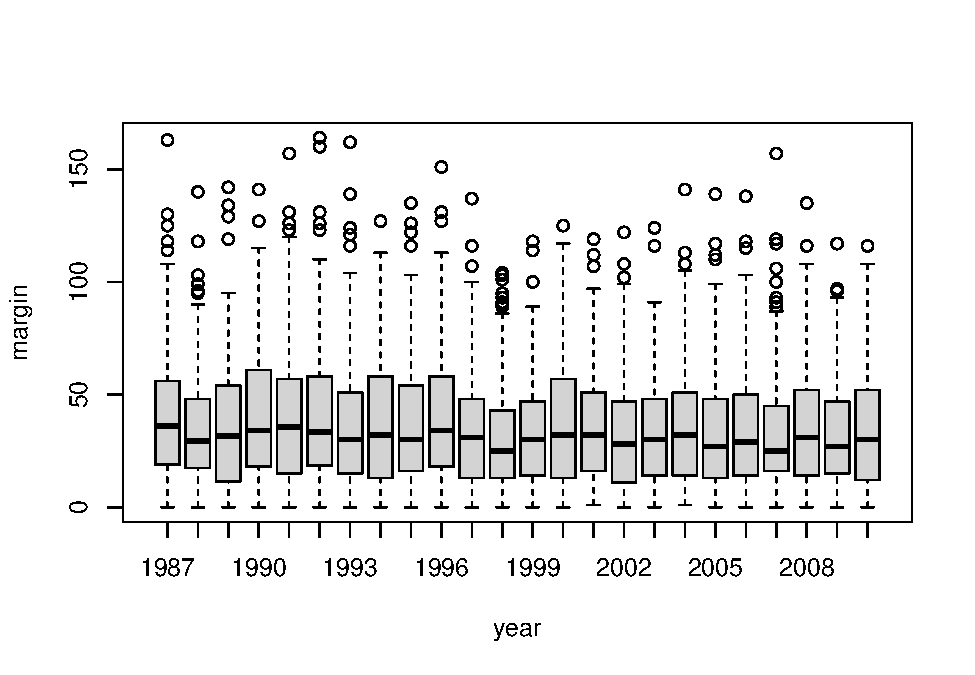
\includegraphics{schuster-statistics-remix_files/figure-latex/multipleboxplots-1.pdf}
\caption{\label{fig:multipleboxplots}Boxplots showing the AFL winning margins for the 24 years from 1987 to 2010 inclusive. This is the default plot created by R, with no annotations added and no changes to the visual design. It's pretty readable, though at a minimum you'd want to include some basic annotations labelling the axes. Compare and contrast with Figure \ref{fig:multipleboxplots2}}
\end{figure}

Even this, the default version of the plot, gives a sense of why it's sometimes useful to choose boxplots instead of histograms. Even before taking the time to turn this basic output into something more readable, it's possible to get a good sense of what the data look like from year to year without getting overwhelmed with too much detail. Now imagine what would have happened if I'd tried to cram 24 histograms into this space: no chance at all that the reader is going to learn anything useful.

That being said, the default boxplot leaves a great deal to be desired in terms of visual clarity. The outliers are too visually prominent, the dotted lines look messy, and the interesting content (i.e., the behaviour of the median and the interquartile range across years) gets a little obscured. Fortunately, this is easy to fix, since we've already covered a lot of tools you can use to customise your output. After playing around with several different versions of the plot, the one I settled on is shown in Figure \ref{fig:multipleboxplots2}. The command I used to produce it is long, but not complicated:

\begin{Shaded}
\begin{Highlighting}[]
\FunctionTok{boxplot}\NormalTok{( }\AttributeTok{formula =}\NormalTok{  margin }\SpecialCharTok{\textasciitilde{}}\NormalTok{ year,   }\CommentTok{\# the formula}
           \AttributeTok{data =}\NormalTok{ afl2,                }\CommentTok{\# the data set}
           \AttributeTok{xlab =} \StringTok{"AFL season"}\NormalTok{,        }\CommentTok{\# x axis label}
           \AttributeTok{ylab =} \StringTok{"Winning Margin"}\NormalTok{,    }\CommentTok{\# y axis label}
           \AttributeTok{frame.plot =} \ConstantTok{FALSE}\NormalTok{,         }\CommentTok{\# don\textquotesingle{}t draw a frame}
           \AttributeTok{staplewex =} \DecValTok{0}\NormalTok{,              }\CommentTok{\# don\textquotesingle{}t draw staples}
           \AttributeTok{staplecol =} \StringTok{"white"}\NormalTok{,        }\CommentTok{\# (fixes a tiny display issue)}
           \AttributeTok{boxwex =}\NormalTok{ .}\DecValTok{75}\NormalTok{,               }\CommentTok{\# narrow the boxes slightly}
           \AttributeTok{boxfill =} \StringTok{"grey80"}\NormalTok{,         }\CommentTok{\# lightly shade the boxes}
           \AttributeTok{whisklty =} \DecValTok{1}\NormalTok{,               }\CommentTok{\# solid line for whiskers }
           \AttributeTok{whiskcol =} \StringTok{"grey70"}\NormalTok{,        }\CommentTok{\# dim the whiskers}
           \AttributeTok{boxcol =} \StringTok{"grey70"}\NormalTok{,          }\CommentTok{\# dim the box borders}
           \AttributeTok{outcol =} \StringTok{"grey70"}\NormalTok{,          }\CommentTok{\# dim the outliers}
           \AttributeTok{outpch =} \DecValTok{20}\NormalTok{,                }\CommentTok{\# outliers as solid dots}
           \AttributeTok{outcex =}\NormalTok{ .}\DecValTok{5}\NormalTok{,                }\CommentTok{\# shrink the outliers}
           \AttributeTok{medlty =} \StringTok{"blank"}\NormalTok{,           }\CommentTok{\# no line for the medians}
           \AttributeTok{medpch =} \DecValTok{20}\NormalTok{,                }\CommentTok{\# instead, draw solid dots}
           \AttributeTok{medlwd =} \FloatTok{1.5}                \CommentTok{\# make them larger}
\NormalTok{ )}
\end{Highlighting}
\end{Shaded}

\begin{figure}
\centering
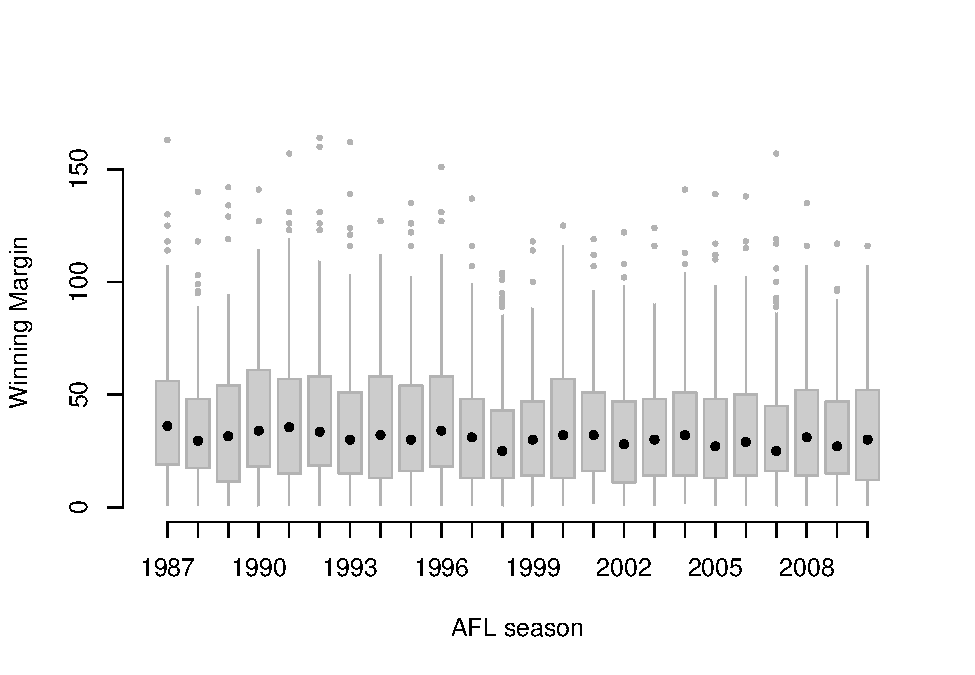
\includegraphics{schuster-statistics-remix_files/figure-latex/multipleboxplots2-1.pdf}
\caption{\label{fig:multipleboxplots2}A cleaned up version of Figure \ref{fig:multipleboxplots}. Notice that I've used a very minimalist design for the boxplots, so as to focus the eye on the medians. I've also converted the medians to solid dots, to convey a sense that year to year variation in the median should be thought of as a single coherent plot (similar to what we did when plotting the \texttt{Fibonacci} variable earlier). The size of outliers has been shrunk, because they aren't actually very interesting. In contrast, I've added a fill colour to the boxes, to make it easier to look at the trend in the interquartile range across years.}
\end{figure}

Of course, given that the command is that long, you might have guessed that I didn't spend ages typing all that rubbish in over and over again. Instead, I wrote a script, which I kept tweaking until it produced the figure that I wanted. We'll talk about scripts later in Section \ref{scripts}, but given the length of the command I thought I'd remind you that there's an easier way of trying out different commands than typing them all in over and over.

\hypertarget{bargraph}{%
\subsection{Bar graphs}\label{bargraph}}

Another form of graph that you often want to plot is the \textbf{\emph{bar graph}}. The main function that you can use in R to draw them is the \texttt{barplot()} function.\footnote{Once again, it's worth noting the link to the generic \texttt{plot()} function. If the \texttt{x} argument to \texttt{plot()} is a factor (and no \texttt{y} argument is given), the result is a bar graph. So you could use \texttt{plot(\ afl.finalists\ )} and get the same output as \texttt{barplot(\ afl.finalists\ )}.} And to illustrate the use of the function, I'll use the \texttt{finalists} variable that I introduced in Section \ref{mode}. What I want to do is draw a bar graph that displays the number of finals that each team has played in over the time spanned by the \texttt{afl} data set. So, let's start by creating a vector that contains this information. I'll use the \texttt{tabulate()} function to do this (which will be discussed properly in Section \ref{freqtables}, since it creates a simple numeric vector:

\begin{Shaded}
\begin{Highlighting}[]
\NormalTok{freq }\OtherTok{\textless{}{-}} \FunctionTok{tabulate}\NormalTok{( afl.finalists )}
\FunctionTok{print}\NormalTok{( freq )}
\end{Highlighting}
\end{Shaded}

\begin{verbatim}
##  [1] 26 25 26 28 32  0  6 39 27 28 28 17  6 24 26 38 24
\end{verbatim}

This isn't exactly the prettiest of frequency tables, of course. I'm only doing it this way so that you can see the \texttt{barplot()} function in it's ``purest'' form: when the input is just an ordinary numeric vector. That being said, I'm obviously going to need the team names to create some labels, so let's create a variable with those. I'll do this using the \texttt{levels()} function, which outputs the names of all the levels of a factor (see Section \ref{factors}:

\begin{Shaded}
\begin{Highlighting}[]
\NormalTok{teams }\OtherTok{\textless{}{-}} \FunctionTok{levels}\NormalTok{( afl.finalists )}
\FunctionTok{print}\NormalTok{( teams )}
\end{Highlighting}
\end{Shaded}

\begin{verbatim}
##  [1] "Adelaide"         "Brisbane"         "Carlton"         
##  [4] "Collingwood"      "Essendon"         "Fitzroy"         
##  [7] "Fremantle"        "Geelong"          "Hawthorn"        
## [10] "Melbourne"        "North Melbourne"  "Port Adelaide"   
## [13] "Richmond"         "St Kilda"         "Sydney"          
## [16] "West Coast"       "Western Bulldogs"
\end{verbatim}

Okay, so now that we have the information we need, let's draw our bar graph. The main argument that you need to specify for a bar graph is the \texttt{height} of the bars, which in our case correspond to the values stored in the \texttt{freq} variable:

\begin{Shaded}
\begin{Highlighting}[]
\FunctionTok{barplot}\NormalTok{( }\AttributeTok{height =}\NormalTok{ freq )  }\CommentTok{\# specifying the argument name}
\FunctionTok{barplot}\NormalTok{( freq )           }\CommentTok{\# the lazier version}
\end{Highlighting}
\end{Shaded}

Either of these two commands will produce the simple bar graph shown in Figure \ref{fig:bar1a}.

\begin{figure}
\centering
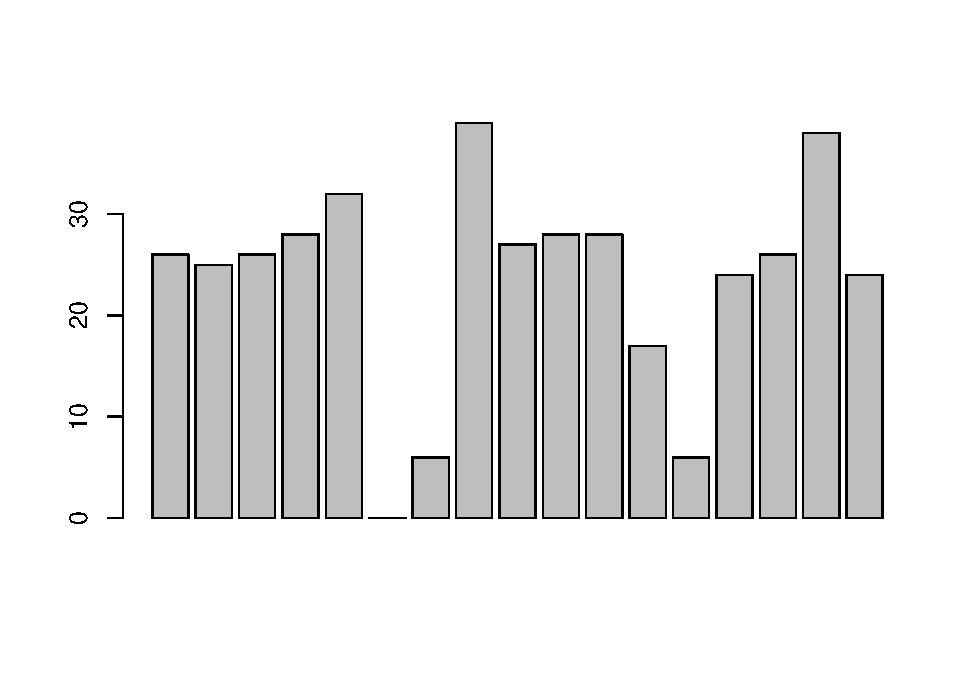
\includegraphics{schuster-statistics-remix_files/figure-latex/bar1a-1.pdf}
\caption{\label{fig:bar1a}the simplest version of a bargraph, containing the data but no labels}
\end{figure}

As you can see, R has drawn a pretty minimal plot. It doesn't have any labels, obviously, because we didn't actually tell the \texttt{barplot()} function what the labels are! To do this, we need to specify the \texttt{names.arg} argument. The \texttt{names.arg} argument needs to be a vector of character strings containing the text that needs to be used as the label for each of the items. In this case, the \texttt{teams} vector is exactly what we need, so the command we're looking for is:

\begin{Shaded}
\begin{Highlighting}[]
    \FunctionTok{barplot}\NormalTok{( }\AttributeTok{height =}\NormalTok{ freq, }\AttributeTok{names.arg =}\NormalTok{ teams ) }
\end{Highlighting}
\end{Shaded}

\begin{figure}
\centering
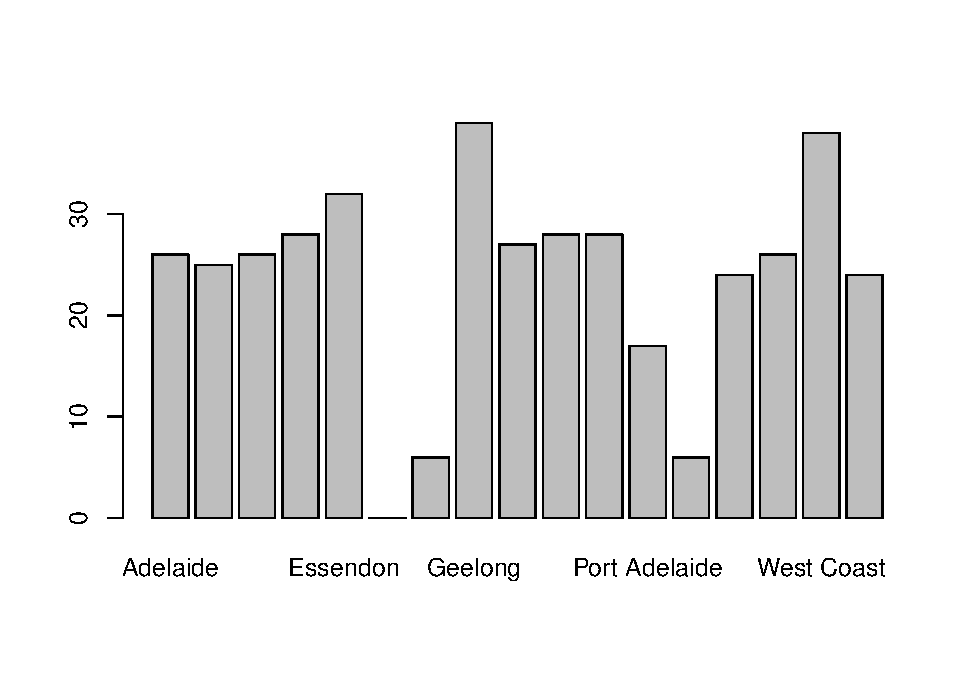
\includegraphics{schuster-statistics-remix_files/figure-latex/bar1b-1.pdf}
\caption{\label{fig:bar1b}we've added the labels, but because the text runs horizontally R only includes a few of them}
\end{figure}

This is an improvement, but not much of an improvement. R has only included a few of the labels, because it can't fit them in the plot. This is the same behaviour we saw earlier with the multiple-boxplot graph in Figure \ref{fig:multipleboxplots}. However, in Figure \ref{fig:multipleboxplots} it wasn't an issue: it's pretty obvious from inspection that the two unlabelled plots in between 1987 and 1990 must correspond to the data from 1988 and 1989. However, the fact that \texttt{barplot()} has omitted the names of every team in between Adelaide and Fitzroy is a lot more problematic.

The simplest way to fix this is to rotate the labels, so that the text runs vertically not horizontally. To do this, we need to alter set the \texttt{las} parameter, which I discussed briefly in Section \ref{introplotting}. What I'll do is tell R to rotate the text so that it's always perpendicular to the axes (i.e., I'll set \texttt{las\ =\ 2}). When I do that, as per the following command\ldots{}

\begin{Shaded}
\begin{Highlighting}[]
    \FunctionTok{barplot}\NormalTok{(}\AttributeTok{height =}\NormalTok{ freq,  }\CommentTok{\# the frequencies}
            \AttributeTok{names.arg =}\NormalTok{ teams,  }\CommentTok{\# the label}
            \AttributeTok{las =} \DecValTok{2}\NormalTok{)            }\CommentTok{\# rotate the labels}
\end{Highlighting}
\end{Shaded}

\begin{figure}
\centering
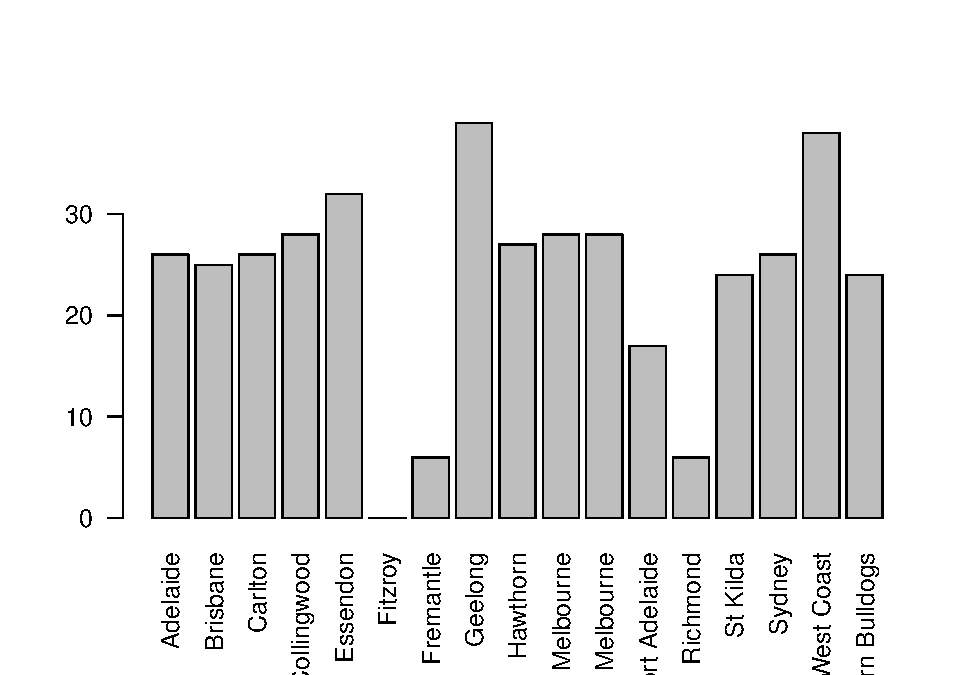
\includegraphics{schuster-statistics-remix_files/figure-latex/bar1c-1.pdf}
\caption{\label{fig:bar1c}we've rotated the labels, but now the text is too long to fit}
\end{figure}

\ldots{} the result is the bar graph shown in Figure \ref{fig:bar1c}. We've fixed the problem, but we've created a new one: the axis labels don't quite fit anymore. To fix this, we have to be a bit cleverer again. A simple fix would be to use shorter names rather than the full name of all teams, and in many situations that's probably the right thing to do. However, at other times you really do need to create a bit more space to add your labels, so I'll show you how to do that.

\hypertarget{saveimage}{%
\subsection{Saving image files using R and Rstudio}\label{saveimage}}

Hold on, you might be thinking. What's the good of being able to draw pretty pictures in R if I can't save them and send them to friends to brag about how awesome my data is? How do I save the picture? This is another one of those situations where the easiest thing to do is to use the RStudio tools.

If you're running R through Rstudio, then the easiest way to save your image is to click on the ``Export'' button in the Plot panel (i.e., the area in Rstudio where all the plots have been appearing). When you do that you'll see a menu that contains the options ``Save Plot as PDF'' and ``Save Plot as Image''. Either version works. Both will bring up dialog boxes that give you a few options that you can play with, but besides that it's pretty simple.

This works pretty nicely for most situations. So, unless you're filled with a burning desire to learn the low level details, feel free to skip the rest of this section.

\hypertarget{summary-2}{%
\subsection{Summary}\label{summary-2}}

Calculating some basic descriptive statistics is one of the very first things you do when analysing real data, and descriptive statistics are much simpler to understand than inferential statistics, so like every other statistics textbook I've started with descriptives. In this chapter, we talked about the following topics:

\begin{itemize}
\tightlist
\item
  \emph{Measures of central tendency}. Broadly speaking, central tendency measures tell you where the data are. There's three measures that are typically reported in the literature: the mean, median and mode. (Section \ref{centraltendency})
\item
  \emph{Measures of variability}. In contrast, measures of variability tell you about how ``spread out'' the data are. The key measures are: range, standard deviation, interquartile reange (Section \ref{var})
\item
  \emph{Getting summaries of variables in R}. Since this book focuses on doing data analysis in R, we spent a bit of time talking about how descriptive statistics are computed in R. (Section \ref{summary} and \ref{groupdescriptives})
\item
  \emph{Basic overview to R graphics}. In Section \ref{rgraphics} we talked about how graphics in R are organised, and then moved on to the basics of how they're drawn in Section \ref{introplotting}.
\item
  \emph{Common plots}. Much of the chapter was focused on standard graphs that statisticians like to produce: histograms (Section \ref{hist}), boxplots (Section \ref{boxplots}), and bar graphs (Section \ref{bargraph}).
\end{itemize}

A traditional first course in statistics spends only a small proportion of the class on descriptive statistics, maybe one or two lectures at most. The vast majority of the lecturer's time is spent on inferential statistics, because that's where all the hard stuff is. That makes sense, but it hides the practical everyday importance of choosing good descriptives.

\textbf{Dave note:} With this chapter, I condensed two of \citet{Navarro2018}'s chapters: descriptive stats and visualizations. For our course, the tools we need at this moment are the ones that help us describe single variables. We will introduce additional tools for summarizing and visualizing bivariate (two variable) data a bit later in the course, when we need them. And, if you do not feel comfortable with every customiziation option presented here, do not be concerned. For now, if you can generate histograms, bar charts, and the like, you have what you need. We will learn more about customizing these graphs for presentations later, as well.

\hypertarget{inferential-statistics-the-central-limit-theorem}{%
\chapter{Inferential statistics: The Central Limit Theorem}\label{inferential-statistics-the-central-limit-theorem}}

\hypertarget{videos-2}{%
\section{Videos}\label{videos-2}}

\href{https://www.youtube.com/watch?v=GEFxFVESQXc}{Video: Are you a Bayesian or a Frequentist?}

\href{https://www.youtube.com/watch?v=be9e-Q-jC-0}{Video: Sampling Methods}

\href{https://www.youtube.com/watch?v=_BiVb6neUP0}{Video: Estimation and Confidence Intervals}

\href{https://youtu.be/qpioCUPvyHY}{Video: The central limit theorem}

\hypertarget{estimation}{%
\section{Introduction}\label{estimation}}

Text by \citet{Navarro2018}

The role of descriptive statistics is to concisely summarise what we \emph{do} know. In contrast, the purpose of inferential statistics is to ``learn what we do not know from what we do''. We are in a good position to think about the problem of statistical inference. What kinds of things would we like to learn about? And how do we learn them? These are the questions that lie at the heart of inferential statistics, and they are traditionally divided into two ``big ideas'': estimation and hypothesis testing. The goal in this chapter is to introduce the first of these big ideas, estimation theory, but I'm going to witter on about probability and sampling theory first because estimation theory doesn't make sense until you understand probability and sampling . As a consequence, this chapter divides naturally into two parts Sections \ref{srs} through \ref{samplesandclt} are focused on sampling theory, and Sections \ref{pointestimates} and \ref{ci} make use of sampling theory to discuss how statisticians think about estimation.

\hypertarget{probstats}{%
\section{How are probability and statistics different?}\label{probstats}}

Text by \citet{Navarro2018}
Before we start talking about probability theory, it's helpful to spend a moment thinking about the relationship between probability and statistics. The two disciplines are closely related but they're not identical. Probability theory is ``the doctrine of chances''. It's a branch of mathematics that tells you how often different kinds of events will happen. For example, all of these questions are things you can answer using probability theory:

\begin{itemize}
\tightlist
\item
  What are the chances of a fair coin coming up heads 10 times in a row?
\item
  If I roll two six sided dice, how likely is it that I'll roll two sixes?
\item
  How likely is it that five cards drawn from a perfectly shuffled deck will all be hearts?
\item
  What are the chances that I'll win the lottery?
\end{itemize}

Notice that all of these questions have something in common. In each case the ``truth of the world'' is known, and my question relates to the ``what kind of events'' will happen. In the first question I \emph{know} that the coin is fair, so there's a 50\% chance that any individual coin flip will come up heads. In the second question, I \emph{know} that the chance of rolling a 6 on a single die is 1 in 6. In the third question I \emph{know} that the deck is shuffled properly. And in the fourth question, I \emph{know} that the lottery follows specific rules. You get the idea. The critical point is that probabilistic questions start with a known \textbf{\emph{model}} of the world, and we use that model to do some calculations. The underlying model can be quite simple. For instance, in the coin flipping example, we can write down the model like this:
\[
P(\mbox{heads}) = 0.5
\]
which you can read as ``the probability of heads is 0.5''. As we'll see later, in the same way that percentages are numbers that range from 0\% to 100\%, probabilities are just numbers that range from 0 to 1. When using this probability model to answer the first question, I don't actually know exactly what's going to happen. Maybe I'll get 10 heads, like the question says. But maybe I'll get three heads. That's the key thing: in probability theory, the \emph{model} is known, but the \emph{data} are not.

So that's probability. What about statistics? Statistical questions work the other way around. In statistics, we \emph{do not} know the truth about the world. All we have is the data, and it is from the data that we want to \emph{learn} the truth about the world. Statistical questions tend to look more like these:

\begin{itemize}
\tightlist
\item
  If my friend flips a coin 10 times and gets 10 heads, are they playing a trick on me?
\item
  If five cards off the top of the deck are all hearts, how likely is it that the deck was shuffled? - If the lottery commissioner's spouse wins the lottery, how likely is it that the lottery was rigged?
\end{itemize}

This time around, the only thing we have are data. What I \emph{know} is that I saw my friend flip the coin 10 times and it came up heads every time. And what I want to \textbf{\emph{infer}} is whether or not I should conclude that what I just saw was actually a fair coin being flipped 10 times in a row, or whether I should suspect that my friend is playing a trick on me. The data I have look like this:

\begin{verbatim}
H H H H H H H H H H H
\end{verbatim}

and what I'm trying to do is work out which ``model of the world'' I should put my trust in. If the coin is fair, then the model I should adopt is one that says that the probability of heads is 0.5; that is, \(P(\mbox{heads}) = 0.5\). If the coin is not fair, then I should conclude that the probability of heads is \emph{not} 0.5, which we would write as \(P(\mbox{heads}) \neq 0.5\). In other words, the statistical inference problem is to figure out which of these probability models is right. Clearly, the statistical question isn't the same as the probability question, but they're deeply connected to one another. Because of this, a good introduction to statistical theory will start with a discussion of what probability is and how it works.

\hypertarget{probmeaning}{%
\section{What does probability mean?}\label{probmeaning}}

Text by \citet{Navarro2018}

Let's start with the first of these questions. What is ``probability''? It might seem surprising to you, but while statisticians and mathematicians (mostly) agree on what the \emph{rules} of probability are, there's much less of a consensus on what the word really \emph{means}. It seems weird because we're all very comfortable using words like ``chance'', ``likely'', ``possible'' and ``probable'', and it doesn't seem like it should be a very difficult question to answer. If you had to explain ``probability'' to a five year old, you could do a pretty good job. But if you've ever had that experience in real life, you might walk away from the conversation feeling like you didn't quite get it right, and that (like many everyday concepts) it turns out that you don't \emph{really} know what it's all about.

So I'll have a go at it. Let's suppose I want to bet on a soccer game between two teams of robots, \emph{Arduino Arsenal} and \emph{C Milan}. After thinking about it, I decide that there is an 80\% probability that \emph{Arduino Arsenal} winning. What do I mean by that? Here are three possibilities\ldots{}

\begin{itemize}
\tightlist
\item
  They're robot teams, so I can make them play over and over again, and if I did that, \emph{Arduino Arsenal} would win 8 out of every 10 games on average.
\item
  For any given game, I would only agree that betting on this game is only ``fair'' if a \$1 bet on \emph{C Milan} gives a \$5 payoff (i.e.~I get my \$1 back plus a \$4 reward for being correct), as would a \$4 bet on \emph{Arduino Arsenal} (i.e., my \$4 bet plus a \$1 reward).
\item
  My subjective ``belief'' or ``confidence'' in an \emph{Arduino Arsenal} victory is four times as strong as my belief in a \emph{C Milan} victory.
\end{itemize}

Each of these seems sensible. However they're not identical, and not every statistician would endorse all of them. The reason is that there are different statistical ideologies (yes, really!) and depending on which one you subscribe to, you might say that some of those statements are meaningless or irrelevant. In this section, I give a brief introduction the two main approaches that exist in the literature. These are by no means the only approaches, but they're the two big ones.

\hypertarget{the-frequentist-view}{%
\subsection{The frequentist view}\label{the-frequentist-view}}

The first of the two major approaches to probability, and the more dominant one in statistics, is referred to as the \textbf{\emph{frequentist view}}, and it defines probability as a \textbf{\emph{long-run frequency}}. Suppose we were to try flipping a fair coin, over and over again. By definition, this is a coin that has \(P(H) = 0.5\). What might we observe? One possibility is that the first 20 flips might look like this:

\begin{verbatim}
T,H,H,H,H,T,T,H,H,H,H,T,H,H,T,T,T,T,T,H
\end{verbatim}

In this case 11 of these 20 coin flips (55\%) came up heads. Now suppose that I'd been keeping a running tally of the number of heads (which I'll call \(N_H\)) that I've seen, across the first \(N\) flips, and calculate the proportion of heads \(N_H / N\) every time. Here's what I'd get (I did literally flip coins to produce this!):

\begin{tabular}{r|r|r}
\hline
number.of.flips & number.of.heads & proportion\\
\hline
1 & 0 & 0.00\\
\hline
2 & 1 & 0.50\\
\hline
3 & 2 & 0.67\\
\hline
4 & 3 & 0.75\\
\hline
5 & 4 & 0.80\\
\hline
6 & 4 & 0.67\\
\hline
7 & 4 & 0.57\\
\hline
8 & 5 & 0.63\\
\hline
9 & 6 & 0.67\\
\hline
10 & 7 & 0.70\\
\hline
11 & 8 & 0.73\\
\hline
12 & 8 & 0.67\\
\hline
13 & 9 & 0.69\\
\hline
14 & 10 & 0.71\\
\hline
15 & 10 & 0.67\\
\hline
16 & 10 & 0.63\\
\hline
17 & 10 & 0.59\\
\hline
18 & 10 & 0.56\\
\hline
19 & 10 & 0.53\\
\hline
20 & 11 & 0.55\\
\hline
\end{tabular}

Notice that at the start of the sequence, the \emph{proportion} of heads fluctuates wildly, starting at .00 and rising as high as .80. Later on, one gets the impression that it dampens out a bit, with more and more of the values actually being pretty close to the ``right'' answer of .50. This is the frequentist definition of probability in a nutshell: flip a fair coin over and over again, and as \(N\) grows large (approaches infinity, denoted \(N\rightarrow \infty\)), the proportion of heads will converge to 50\%. There are some subtle technicalities that the mathematicians care about, but qualitatively speaking, that's how the frequentists define probability. Unfortunately, I don't have an infinite number of coins, or the infinite patience required to flip a coin an infinite number of times. However, I do have a computer, and computers excel at mindless repetitive tasks. So I asked my computer to simulate flipping a coin 1000 times, and then drew a picture of what happens to the proportion \(N_H / N\) as \(N\) increases. Actually, I did it four times, just to make sure it wasn't a fluke. The results are shown in Figure \ref{fig:frequentistprobability}. As you can see, the \emph{proportion of observed heads} eventually stops fluctuating, and settles down; when it does, the number at which it finally settles is the true probability of heads.

\begin{figure}
\centering
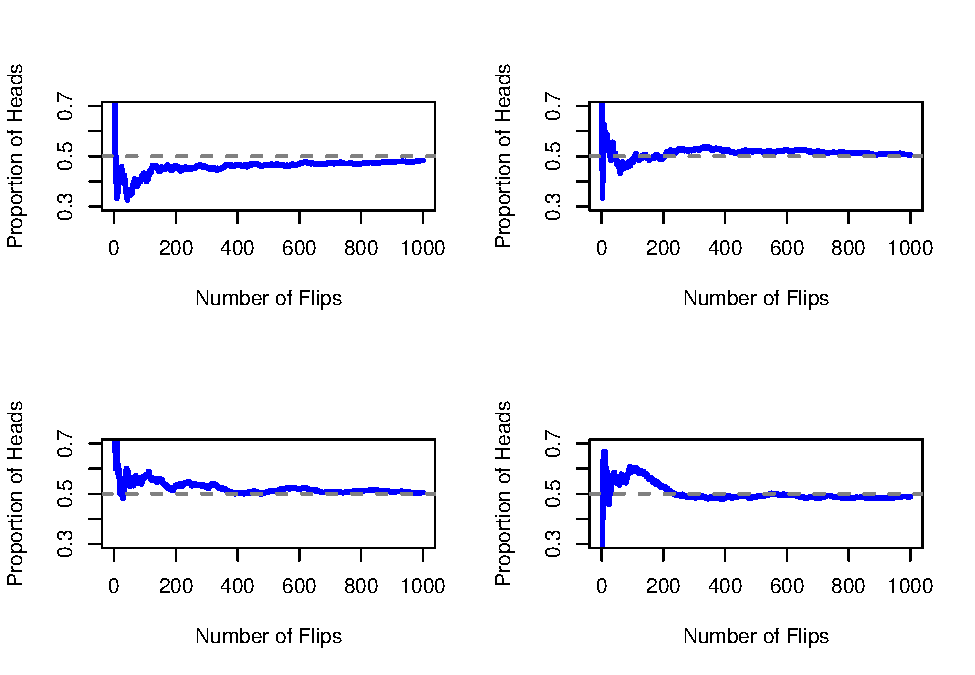
\includegraphics{schuster-statistics-remix_files/figure-latex/frequentistprobability-1.pdf}
\caption{\label{fig:frequentistprobability}An illustration of how frequentist probability works. If you flip a fair coin over and over again, the proportion of heads that you've seen eventually settles down, and converges to the true probability of 0.5. Each panel shows four different simulated experiments: in each case, we pretend we flipped a coin 1000 times, and kept track of the proportion of flips that were heads as we went along. Although none of these sequences actually ended up with an exact value of .5, if we'd extended the experiment for an infinite number of coin flips they would have.}
\end{figure}

The frequentist definition of probability has some desirable characteristics. Firstly, it is objective: the probability of an event is \emph{necessarily} grounded in the world. The only way that probability statements can make sense is if they refer to (a sequence of) events that occur in the physical universe.\footnote{This doesn't mean that frequentists can't make hypothetical statements, of course; it's just that if you want to make a statement about probability, then it must be possible to redescribe that statement in terms of a sequence of potentially observable events, and the relative frequencies of different outcomes that appear within that sequence.} Secondly, it is unambiguous: any two people watching the same sequence of events unfold, trying to calculate the probability of an event, must inevitably come up with the same answer. However, it also has undesirable characteristics. Firstly, infinite sequences don't exist in the physical world. Suppose you picked up a coin from your pocket and started to flip it. Every time it lands, it impacts on the ground. Each impact wears the coin down a bit; eventually, the coin will be destroyed. So, one might ask whether it really makes sense to pretend that an ``infinite'' sequence of coin flips is even a meaningful concept, or an objective one. We can't say that an ``infinite sequence'' of events is a real thing in the physical universe, because the physical universe doesn't allow infinite anything. More seriously, the frequentist definition has a narrow scope. There are lots of things out there that human beings are happy to assign probability to in everyday language, but cannot (even in theory) be mapped onto a hypothetical sequence of events. For instance, if a meteorologist comes on TV and says, ``the probability of rain in Adelaide on 2 November 2048 is 60\%'' we humans are happy to accept this. But it's not clear how to define this in frequentist terms. There's only one city of Adelaide, and only 2 November 2048. There's no infinite sequence of events here, just a once-off thing. Frequentist probability genuinely \emph{forbids} us from making probability statements about a single event. From the frequentist perspective, it will either rain tomorrow or it will not; there is no ``probability'' that attaches to a single non-repeatable event. Now, it should be said that there are some very clever tricks that frequentists can use to get around this. One possibility is that what the meteorologist means is something like this: ``There is a category of days for which I predict a 60\% chance of rain; if we look only across those days for which I make this prediction, then on 60\% of those days it will actually rain''. It's very weird and counterintuitive to think of it this way, but you do see frequentists do this sometimes. And it \emph{will} come up later in this book (see Section \ref{ci}).

\hypertarget{the-bayesian-view}{%
\subsection{The Bayesian view}\label{the-bayesian-view}}

The \textbf{\emph{Bayesian view}} of probability is often called the subjectivist view, and it is a minority view among statisticians, but one that has been steadily gaining traction for the last several decades. There are many flavours of Bayesianism, making hard to say exactly what ``the'' Bayesian view is. The most common way of thinking about subjective probability is to define the probability of an event as the \textbf{\emph{degree of belief}} that an intelligent and rational agent assigns to that truth of that event. From that perspective, probabilities don't exist in the world, but rather in the thoughts and assumptions of people and other intelligent beings.
However, in order for this approach to work, we need some way of operationalising ``degree of belief''. One way that you can do this is to formalise it in terms of ``rational gambling'', though there are many other ways. Suppose that I believe that there's a 60\% probability of rain tomorrow. If someone offers me a bet: if it rains tomorrow, then I win \$5, but if it doesn't rain then I lose \$5. Clearly, from my perspective, this is a pretty good bet. On the other hand, if I think that the probability of rain is only 40\%, then it's a bad bet to take. Thus, we can operationalise the notion of a ``subjective probability'' in terms of what bets I'm willing to accept.

What are the advantages and disadvantages to the Bayesian approach? The main advantage is that it allows you to assign probabilities to any event you want to. You don't need to be limited to those events that are repeatable. The main disadvantage (to many people) is that we can't be purely objective -- specifying a probability requires us to specify an entity that has the relevant degree of belief. This entity might be a human, an alien, a robot, or even a statistician, but there has to be an intelligent agent out there that believes in things. To many people this is uncomfortable: it seems to make probability arbitrary. While the Bayesian approach does require that the agent in question be rational (i.e., obey the rules of probability), it does allow everyone to have their own beliefs; I can believe the coin is fair and you don't have to, even though we're both rational. The frequentist view doesn't allow any two observers to attribute different probabilities to the same event: when that happens, then at least one of them must be wrong. The Bayesian view does not prevent this from occurring. Two observers with different background knowledge can legitimately hold different beliefs about the same event. In short, where the frequentist view is sometimes considered to be too narrow (forbids lots of things that that we want to assign probabilities to), the Bayesian view is sometimes thought to be too broad (allows too many differences between observers).

\hypertarget{whats-the-difference-and-who-is-right}{%
\subsection{What's the difference? And who is right?}\label{whats-the-difference-and-who-is-right}}

Now that you've seen each of these two views independently, it's useful to make sure you can compare the two. Go back to the hypothetical robot soccer game at the start of the section. What do you think a frequentist and a Bayesian would say about these three statements? Which statement would a frequentist say is the correct definition of probability? Which one would a Bayesian do? Would some of these statements be meaningless to a frequentist or a Bayesian? If you've understood the two perspectives, you should have some sense of how to answer those questions.

Okay, assuming you understand the different, you might be wondering which of them is \emph{right}? Honestly, I don't know that there is a right answer. As far as I can tell there's nothing mathematically incorrect about the way frequentists think about sequences of events, and there's nothing mathematically incorrect about the way that Bayesians define the beliefs of a rational agent. In fact, when you dig down into the details, Bayesians and frequentists actually agree about a lot of things. Many frequentist methods lead to decisions that Bayesians agree a rational agent would make. Many Bayesian methods have very good frequentist properties.

For the most part, I'm a pragmatist so I'll use any statistical method that I trust. As it turns out, that makes me prefer Bayesian methods, for reasons I'll explain towards the end of the book, but I'm not fundamentally opposed to frequentist methods. Not everyone is quite so relaxed. For instance, consider Sir Ronald Fisher, one of the towering figures of 20th century statistics and a vehement opponent to all things Bayesian, whose paper on the mathematical foundations of statistics referred to Bayesian probability as ``an impenetrable jungle {[}that{]} arrests progress towards precision of statistical concepts'' \citet{Fisher1922b}. Or the psychologist Paul Meehl, who suggests that relying on frequentist methods could turn you into ``a potent but sterile intellectual rake who leaves in his merry path a long train of ravished maidens but no viable scientific offspring'' \citet{Meehl1967}. The history of statistics, as you might gather, is not devoid of entertainment.

In any case, while I personally prefer the Bayesian view, the majority of statistical analyses are based on the frequentist approach. My reasoning is pragmatic: the goal of this book is to cover roughly the same territory as a typical undergraduate stats class in psychology, and if you want to understand the statistical tools used by most psychologists, you'll need a good grasp of frequentist methods. I promise you that this isn't wasted effort. Even if you end up wanting to switch to the Bayesian perspective, you really should read through at least one book on the ``orthodox'' frequentist view. And since R is the most widely used statistical language for Bayesians, you might as well read a book that uses R. Besides, I won't completely ignore the Bayesian perspective. Every now and then I'll add some commentary from a Bayesian point of view.

\hypertarget{srs}{%
\section{Samples, populations and sampling}\label{srs}}

Text by \citet{Navarro2018}

In the prelude to Part I discussed the riddle of induction, and highlighted the fact that \emph{all} learning requires you to make assumptions. Accepting that this is true, our first task to come up with some fairly general assumptions about data that make sense. This is where \textbf{\emph{sampling theory}} comes in. If probability theory is the foundations upon which all statistical theory builds, sampling theory is the frame around which you can build the rest of the house. Sampling theory plays a huge role in specifying the assumptions upon which your statistical inferences rely. And in order to talk about ``making inferences'' the way statisticians think about it, we need to be a bit more explicit about what it is that we're drawing inferences \emph{from} (the sample) and what it is that we're drawing inferences \emph{about} (the population).

In almost every situation of interest, what we have available to us as researchers is a \textbf{\emph{sample}} of data. We might have run experiment with some number of participants; a polling company might have phoned some number of people to ask questions about voting intentions; etc. Regardless: the data set available to us is finite, and incomplete. We can't possibly get every person in the world to do our experiment; a polling company doesn't have the time or the money to ring up every voter in the country etc. In our earlier discussion of descriptive statistics (Chapter \ref{descriptives}, this sample was the only thing we were interested in. Our only goal was to find ways of describing, summarising and graphing that sample. This is about to change.

\hypertarget{pop}{%
\subsection{Defining a population}\label{pop}}

A sample is a concrete thing. You can open up a data file, and there's the data from your sample. A \textbf{\emph{population}}, on the other hand, is a more abstract idea. It refers to the set of all possible people, or all possible observations, that you want to draw conclusions about, and is generally \emph{much} bigger than the sample. In an ideal world, the researcher would begin the study with a clear idea of what the population of interest is, since the process of designing a study and testing hypotheses about the data that it produces does depend on the population about which you want to make statements. However, that doesn't always happen in practice: usually the researcher has a fairly vague idea of what the population is and designs the study as best he/she can on that basis.

Sometimes it's easy to state the population of interest. For instance, in the ``polling company'' example that opened the chapter, the population consisted of all voters enrolled at the a time of the study -- millions of people. The sample was a set of 1000 people who all belong to that population. In most situations the situation is much less simple. In a typical a psychological experiment, determining the population of interest is a bit more complicated. Suppose I run an experiment using 100 undergraduate students as my participants. My goal, as a cognitive scientist, is to try to learn something about how the mind works. So, which of the following would count as ``the population'':

\begin{itemize}
\tightlist
\item
  All of the undergraduate psychology students at the University of Adelaide?
\item
  Undergraduate psychology students in general, anywhere in the world?
\item
  Australians currently living?
\item
  Australians of similar ages to my sample?
\item
  Anyone currently alive?
\item
  Any human being, past, present or future?
\item
  Any biological organism with a sufficient degree of intelligence operating in a terrestrial environment?
\item
  Any intelligent being?
\end{itemize}

Each of these defines a real group of mind-possessing entities, all of which might be of interest to me as a cognitive scientist, and it's not at all clear which one ought to be the true population of interest. As another example, consider the Wellesley-Croker game that we discussed in the prelude. The sample here is a specific sequence of 12 wins and 0 losses for Wellesley. What is the population?

\begin{itemize}
\tightlist
\item
  All outcomes until Wellesley and Croker arrived at their destination?
\item
  All outcomes if Wellesley and Croker had played the game for the rest of their lives?
\item
  All outcomes if Wellseley and Croker lived forever and played the game until the world ran out of hills?
\item
  All outcomes if we created an infinite set of parallel universes and the Wellesely/Croker pair made guesses about the same 12 hills in each universe?
\end{itemize}

Again, it's not obvious what the population is.

\hypertarget{simple-random-samples}{%
\subsection{Simple random samples}\label{simple-random-samples}}

\begin{figure}
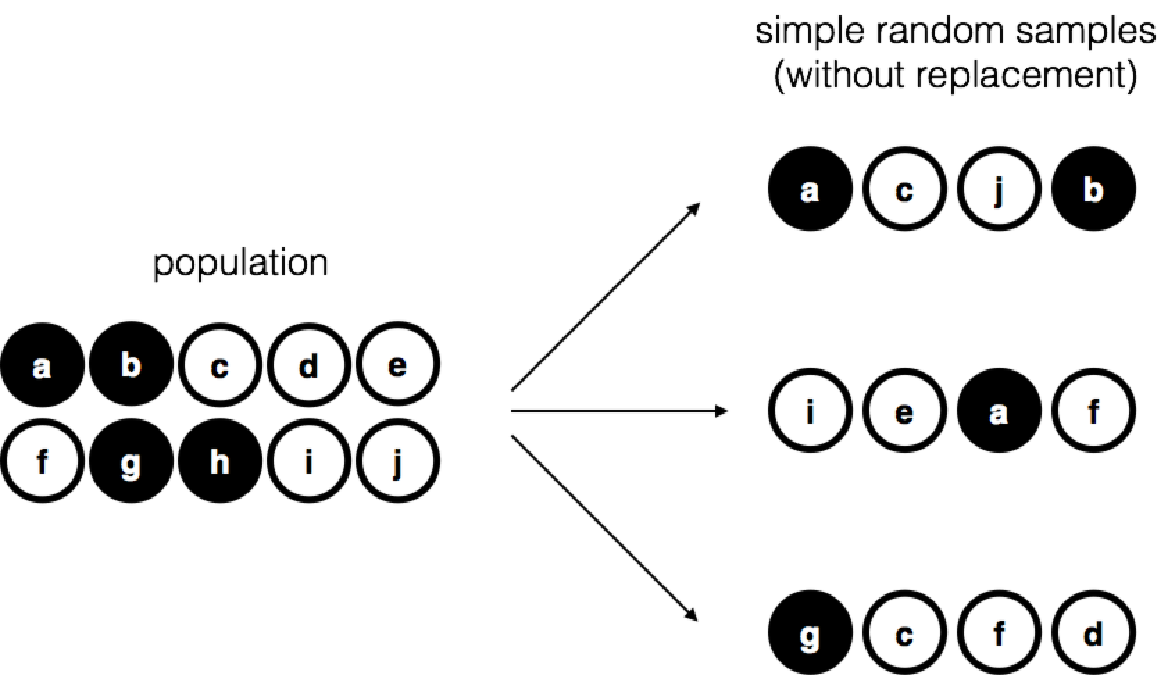
\includegraphics[width=16.24in]{/Users/dave/Documents/GitHub/stats-remix-advanced/img/estimation/srs1} \caption{Simple random sampling without replacement from a finite population}\label{fig:srs1}
\end{figure}

Irrespective of how I define the population, the critical point is that the sample is a subset of the population, and our goal is to use our knowledge of the sample to draw inferences about the properties of the population. The relationship between the two depends on the \emph{procedure} by which the sample was selected. This procedure is referred to as a \textbf{\emph{sampling method}}, and it is important to understand why it matters.

To keep things simple, let's imagine that we have a bag containing 10 chips. Each chip has a unique letter printed on it, so we can distinguish between the 10 chips. The chips come in two colours, black and white. This set of chips is the population of interest, and it is depicted graphically on the left of Figure \ref{fig:srs1}. As you can see from looking at the picture, there are 4 black chips and 6 white chips, but of course in real life we wouldn't know that unless we looked in the bag. Now imagine you run the following ``experiment'': you shake up the bag, close your eyes, and pull out 4 chips without putting any of them back into the bag. First out comes the \(a\) chip (black), then the \(c\) chip (white), then \(j\) (white) and then finally \(b\) (black). If you wanted, you could then put all the chips back in the bag and repeat the experiment, as depicted on the right hand side of Figure \ref{fig:srs1}. Each time you get different results, but the procedure is identical in each case. The fact that the same procedure can lead to different results each time, we refer to it as a \emph{random} process.\footnote{The proper mathematical definition of randomness is extraordinarily technical, and way beyond the scope of this book. We'll be non-technical here and say that a process has an element of randomness to it whenever it is possible to repeat the process and get different answers each time.} However, because we shook the bag before pulling any chips out, it seems reasonable to think that every chip has the same chance of being selected. A procedure in which every member of the population has the same chance of being selected is called a \textbf{\emph{simple random sample}}. The fact that we did \emph{not} put the chips back in the bag after pulling them out means that you can't observe the same thing twice, and in such cases the observations are said to have been sampled \textbf{\emph{without replacement}}.

To help make sure you understand the importance of the sampling procedure, consider an alternative way in which the experiment could have been run. Suppose that my 5-year old son had opened the bag, and decided to pull out four black chips without putting any of them back in the bag. This \emph{biased} sampling scheme is depicted in Figure \ref{fig:brs}. Now consider the evidentiary value of seeing 4 black chips and 0 white chips. Clearly, it depends on the sampling scheme, does it not? If you know that the sampling scheme is biased to select only black chips, then a sample that consists of only black chips doesn't tell you very much about the population! For this reason, statisticians really like it when a data set can be considered a simple random sample, because it makes the data analysis \emph{much} easier.

\begin{figure}
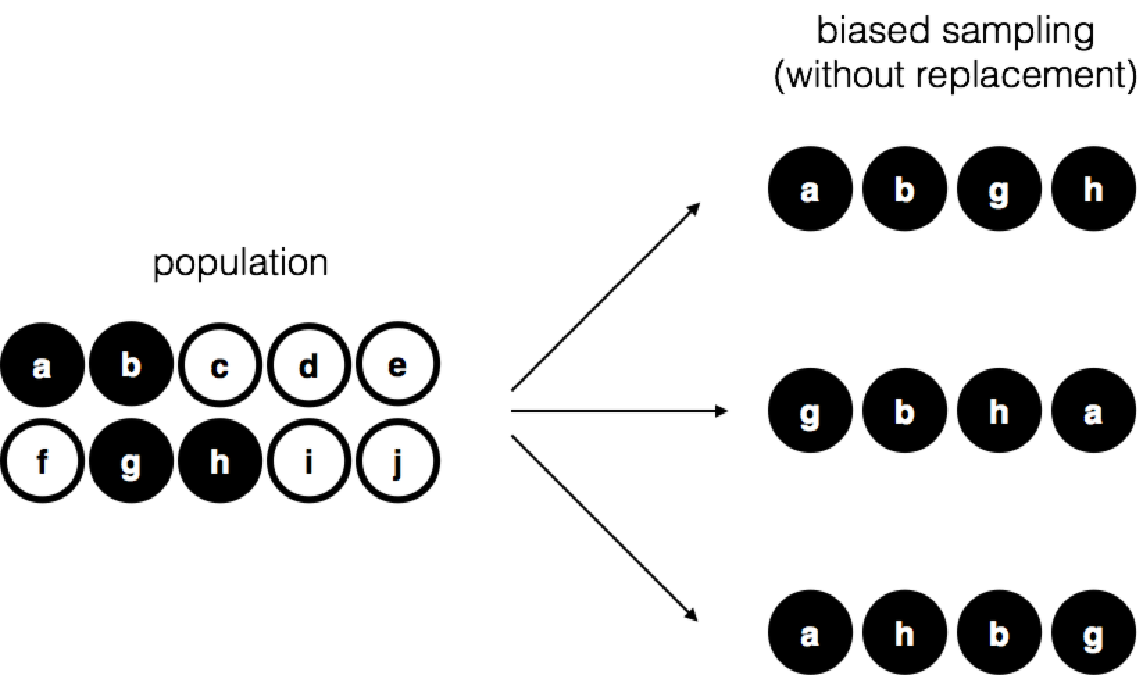
\includegraphics[width=15.89in]{/Users/dave/Documents/GitHub/stats-remix-advanced/img/estimation/brs} \caption{Biased sampling without replacement from a finite population}\label{fig:brs}
\end{figure}

\begin{figure}
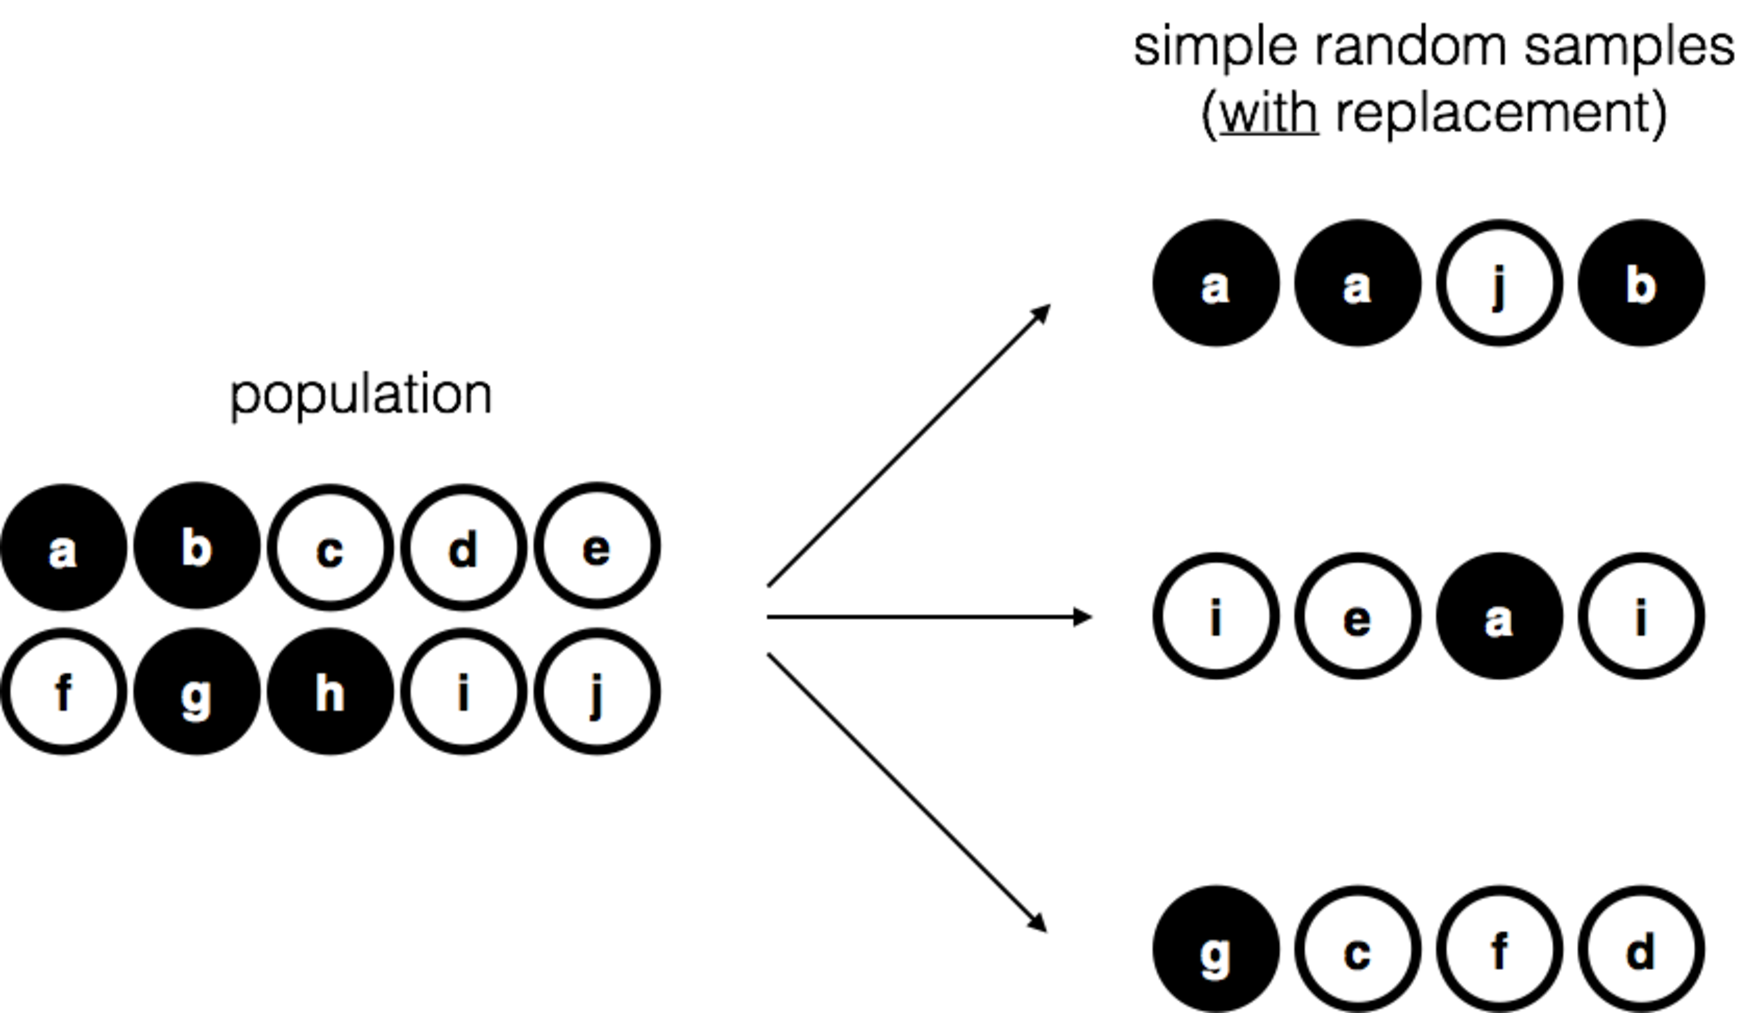
\includegraphics[width=16.24in]{/Users/dave/Documents/GitHub/stats-remix-advanced/img/estimation/srs2} \caption{Simple random sampling *with* replacement from a finite population}\label{fig:srs2}
\end{figure}

A third procedure is worth mentioning. This time around we close our eyes, shake the bag, and pull out a chip. This time, however, we record the observation and then put the chip back in the bag. Again we close our eyes, shake the bag, and pull out a chip. We then repeat this procedure until we have 4 chips. Data sets generated in this way are still simple random samples, but because we put the chips back in the bag immediately after drawing them it is referred to as a sample \textbf{\emph{with replacement}}. The difference between this situation and the first one is that it is possible to observe the same population member multiple times, as illustrated in Figure \ref{fig:srs2}.

In my experience, most psychology experiments tend to be sampling without replacement, because the same person is not allowed to participate in the experiment twice. However, most statistical theory is based on the assumption that the data arise from a simple random sample \emph{with} replacement. In real life, this very rarely matters. If the population of interest is large (e.g., has more than 10 entities!) the difference between sampling with- and without- replacement is too small to be concerned with. The difference between simple random samples and biased samples, on the other hand, is not such an easy thing to dismiss.

\hypertarget{most-samples-are-not-simple-random-samples}{%
\subsection{Most samples are not simple random samples}\label{most-samples-are-not-simple-random-samples}}

As you can see from looking at the list of possible populations that I showed above, it is almost impossible to obtain a simple random sample from most populations of interest. When I run experiments, I'd consider it a minor miracle if my participants turned out to be a random sampling of the undergraduate psychology students at Adelaide university, even though this is by far the narrowest population that I might want to generalise to. A thorough discussion of other types of sampling schemes is beyond the scope of this book, but to give you a sense of what's out there I'll list a few of the more important ones:

\begin{itemize}
\tightlist
\item
  \emph{Stratified sampling}. Suppose your population is (or can be) divided into several different subpopulations, or \emph{strata}. Perhaps you're running a study at several different sites, for example. Instead of trying to sample randomly from the population as a whole, you instead try to collect a separate random sample from each of the strata. Stratified sampling is sometimes easier to do than simple random sampling, especially when the population is already divided into the distinct strata. It can also be more efficient that simple random sampling, especially when some of the subpopulations are rare. For instance, when studying schizophrenia it would be much better to divide the population into two\footnote{Nothing in life is that simple: there's not an obvious division of people into binary categories like ``schizophrenic'' and ``not schizophrenic''. But this isn't a clinical psychology text, so please forgive me a few simplifications here and there.} strata (schizophrenic and not-schizophrenic), and then sample an equal number of people from each group. If you selected people randomly, you would get so few schizophrenic people in the sample that your study would be useless. This specific kind of of stratified sampling is referred to as \emph{oversampling} because it makes a deliberate attempt to over-represent rare groups.
\item
  \emph{Snowball sampling} is a technique that is especially useful when sampling from a ``hidden'' or hard to access population, and is especially common in social sciences. For instance, suppose the researchers want to conduct an opinion poll among transgender people. The research team might only have contact details for a few trans folks, so the survey starts by asking them to participate (stage 1). At the end of the survey, the participants are asked to provide contact details for other people who might want to participate. In stage 2, those new contacts are surveyed. The process continues until the researchers have sufficient data. The big advantage to snowball sampling is that it gets you data in situations that might otherwise be impossible to get any. On the statistical side, the main disadvantage is that the sample is highly non-random, and non-random in ways that are difficult to address. On the real life side, the disadvantage is that the procedure can be unethical if not handled well, because hidden populations are often hidden for a reason. I chose transgender people as an example here to highlight this: if you weren't careful you might end up outing people who don't want to be outed (very, very bad form), and even if you don't make that mistake it can still be intrusive to use people's social networks to study them. It's certainly very hard to get people's informed consent \emph{before} contacting them, yet in many cases the simple act of contacting them and saying ``hey we want to study you'' can be hurtful. Social networks are complex things, and just because you can use them to get data doesn't always mean you should.
\item
  \emph{Convenience sampling} is more or less what it sounds like. The samples are chosen in a way that is convenient to the researcher, and not selected at random from the population of interest. Snowball sampling is one type of convenience sampling, but there are many others. A common example in psychology are studies that rely on undergraduate psychology students. These samples are generally non-random in two respects: firstly, reliance on undergraduate psychology students automatically means that your data are restricted to a single subpopulation. Secondly, the students usually get to pick which studies they participate in, so the sample is a self selected subset of psychology students not a randomly selected subset. In real life, most studies are convenience samples of one form or another. This is sometimes a severe limitation, but not always.
\end{itemize}

\textbf{Dave here}, adding two more sampling methods:

\begin{itemize}
\item
  \emph{Systematic sampling}: Starting from a random point, select every Nth participant.
\item
  \emph{Cluster sampling}: Divide population into clusters or units (such as schools), take a random sample of the clusters (i.e., randomly select a school) and then measure all the participants within the cluster (i.e., measure every student in the school).
\end{itemize}

\hypertarget{how-much-does-it-matter-if-you-dont-have-a-simple-random-sample}{%
\subsection{How much does it matter if you don't have a simple random sample?}\label{how-much-does-it-matter-if-you-dont-have-a-simple-random-sample}}

Okay, so real world data collection tends not to involve nice simple random samples. Does that matter? A little thought should make it clear to you that it \emph{can} matter if your data are not a simple random sample: just think about the difference between Figures \ref{fig:srs1} and \ref{fig:brs}. However, it's not quite as bad as it sounds. Some types of biased samples are entirely unproblematic. For instance, when using a stratified sampling technique you actually \emph{know} what the bias is because you created it deliberately, often to \emph{increase} the effectiveness of your study, and there are statistical techniques that you can use to adjust for the biases you've introduced (not covered in this book!). So in those situations it's not a problem.

More generally though, it's important to remember that random sampling is a means to an end, not the end in itself. Let's assume you've relied on a convenience sample, and as such you can assume it's biased. A bias in your sampling method is only a problem if it causes you to draw the wrong conclusions. When viewed from that perspective, I'd argue that we don't need the sample to be randomly generated in \emph{every} respect: we only need it to be random with respect to the psychologically-relevant phenomenon of interest. Suppose I'm doing a study looking at working memory capacity. In study 1, I actually have the ability to sample randomly from all human beings currently alive, with one exception: I can only sample people born on a Monday. In study 2, I am able to sample randomly from the Australian population. I want to generalise my results to the population of all living humans. Which study is better? The answer, obviously, is study 1. Why? Because we have no reason to think that being ``born on a Monday'' has any interesting relationship to working memory capacity. In contrast, I can think of several reasons why ``being Australian'' might matter. Australia is a wealthy, industrialised country with a very well-developed education system. People growing up in that system will have had life experiences much more similar to the experiences of the people who designed the tests for working memory capacity. This shared experience might easily translate into similar beliefs about how to ``take a test'', a shared assumption about how psychological experimentation works, and so on. These things might actually matter. For instance, ``test taking'' style might have taught the Australian participants how to direct their attention exclusively on fairly abstract test materials relative to people that haven't grown up in a similar environment; leading to a misleading picture of what working memory capacity is.

There are two points hidden in this discussion. Firstly, when designing your own studies, it's important to think about what population you care about, and try hard to sample in a way that is appropriate to that population. In practice, you're usually forced to put up with a ``sample of convenience'' (e.g., psychology lecturers sample psychology students because that's the least expensive way to collect data, and our coffers aren't exactly overflowing with gold), but if so you should at least spend some time thinking about what the dangers of this practice might be.

Secondly, if you're going to criticise someone else's study because they've used a sample of convenience rather than laboriously sampling randomly from the entire human population, at least have the courtesy to offer a specific theory as to \emph{how} this might have distorted the results. Remember, everyone in science is aware of this issue, and does what they can to alleviate it. Merely pointing out that ``the study only included people from group BLAH'' is entirely unhelpful, and borders on being insulting to the researchers, who are \emph{of course} aware of the issue. They just don't happen to be in possession of the infinite supply of time and money required to construct the perfect sample. In short, if you want to offer a responsible critique of the sampling process, then be \emph{helpful}. Rehashing the blindingly obvious truisms that I've been rambling on about in this section isn't helpful.

\hypertarget{population-parameters-and-sample-statistics}{%
\subsection{Population parameters and sample statistics}\label{population-parameters-and-sample-statistics}}

Okay. Setting aside the thorny methodological issues associated with obtaining a random sample and my rather unfortunate tendency to rant about lazy methodological criticism, let's consider a slightly different issue. Up to this point we have been talking about populations the way a scientist might. To a psychologist, a population might be a group of people. To an ecologist, a population might be a group of bears. In most cases the populations that scientists care about are concrete things that actually exist in the real world. Statisticians, however, are a funny lot. On the one hand, they \emph{are} interested in real world data and real science in the same way that scientists are. On the other hand, they also operate in the realm of pure abstraction in the way that mathematicians do. As a consequence, statistical theory tends to be a bit abstract in how a population is defined. In much the same way that psychological researchers operationalise our abstract theoretical ideas in terms of concrete measurements (Section \ref{measurement}, statisticians operationalise the concept of a ``population'' in terms of mathematical objects that they know how to work with. They're called probability distributions.

The idea is quite simple. Let's say we're talking about IQ scores. To a psychologist, the population of interest is a group of actual humans who have IQ scores. A statistician ``simplifies'' this by operationally defining the population as the probability distribution depicted in Figure \ref{fig:IQdist}. IQ tests are designed so that the average IQ is 100, the standard deviation of IQ scores is 15, and the distribution of IQ scores is normal. These values are referred to as the \textbf{\emph{population parameters}} because they are characteristics of the entire population. That is, we say that the population mean \(\mu\) is 100, and the population standard deviation \(\sigma\) is 15.

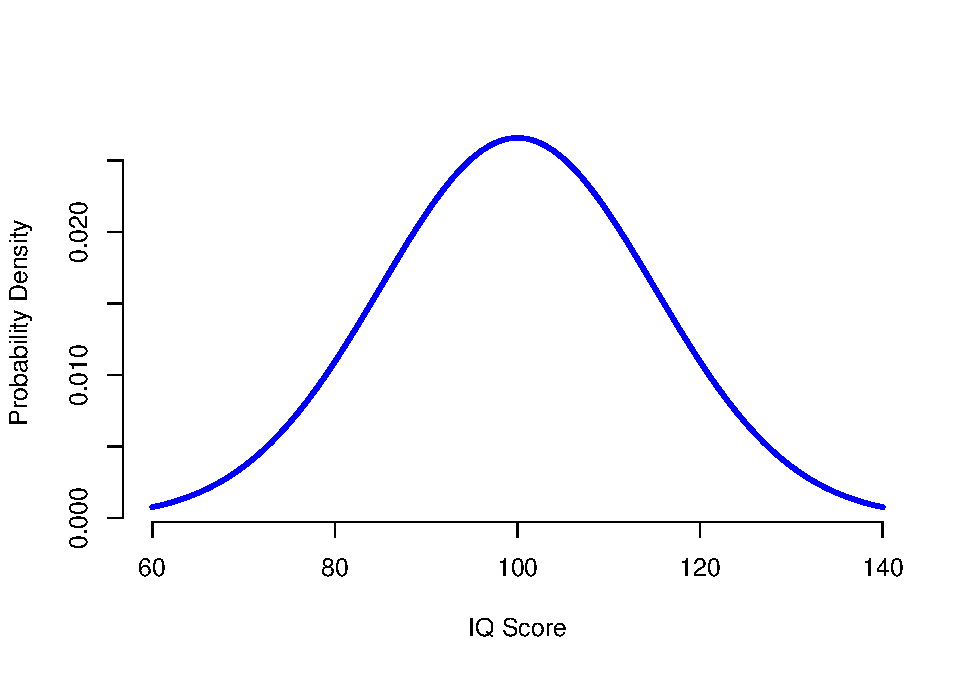
\includegraphics{schuster-statistics-remix_files/figure-latex/IQdist-1.pdf} 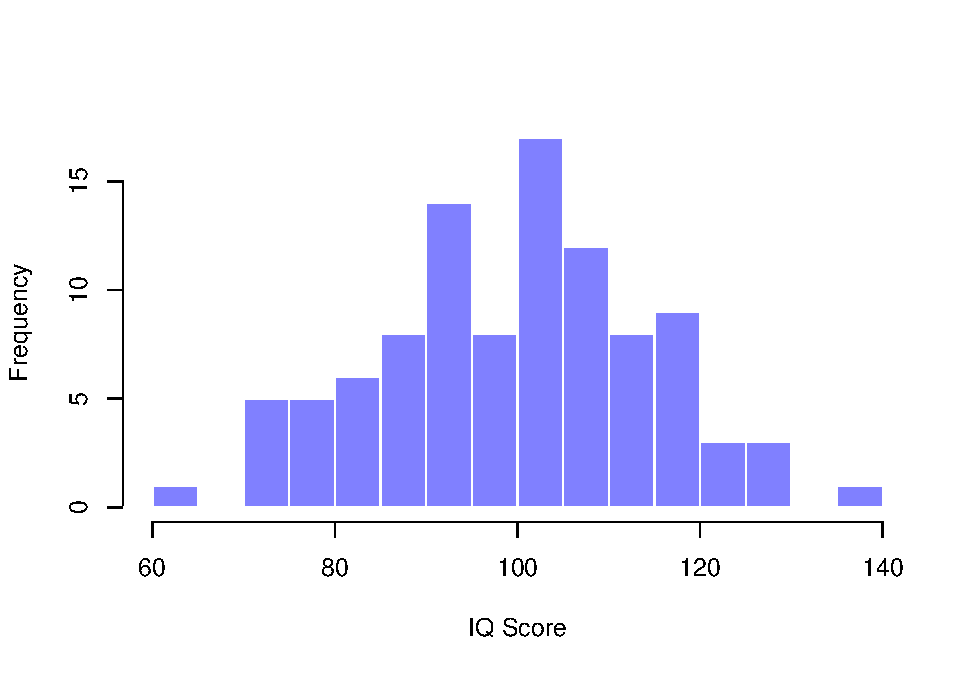
\includegraphics{schuster-statistics-remix_files/figure-latex/IQdist-2.pdf}

\begin{verbatim}
## [1] "n= 100 mean= 99.5919374129665 sd= 15.3971646061716"
\end{verbatim}

\begin{figure}
\centering
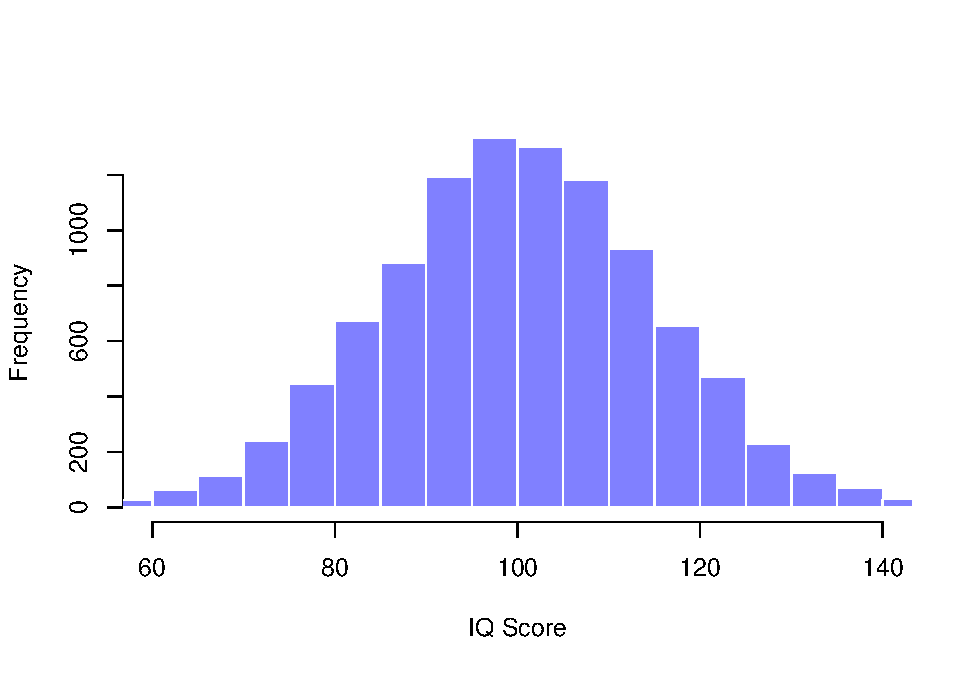
\includegraphics{schuster-statistics-remix_files/figure-latex/IQdist-3.pdf}
\caption{\label{fig:IQdist-3}The population distribution of IQ scores (panel a) and two samples drawn randomly from it. In panel b we have a sample of 100 observations, and panel c we have a sample of 10,000 observations.}
\end{figure}

\begin{verbatim}
## [1] "n= 10000 mean= 99.951621373427 sd= 15.0289049049787"
\end{verbatim}

Now suppose I run an experiment. I select 100 people at random and administer an IQ test, giving me a simple random sample from the population. My sample would consist of a collection of numbers like this:

\begin{verbatim}
                          106 101 98 80 74 ... 107 72 100
\end{verbatim}

Each of these IQ scores is sampled from a normal distribution with mean 100 and standard deviation 15. So if I plot a histogram of the sample, I get something like the one shown in Figure \ref{fig:IQdist}b. As you can see, the histogram is \emph{roughly} the right shape, but it's a very crude approximation to the true population distribution shown in Figure \ref{fig:IQdist}a. When I calculate the mean of my sample, I get a number that is fairly close to the population mean 100 but not identical. In this case, it turns out that the people in my sample have a mean IQ of 98.5, and the standard deviation of their IQ scores is 15.9. These \textbf{\emph{sample statistics}} are properties of my data set, and although they are fairly similar to the true population values, they are not the same. In general, sample statistics are the things you can calculate from your data set, and the population parameters are the things you want to learn about. Later on in this chapter I'll talk about how you can estimate population parameters using your sample statistics (Section \ref{pointestimates} and how to work out how confident you are in your estimates (Section \ref{ci} but before we get to that there's a few more ideas in sampling theory that you need to know about.

\hypertarget{lawlargenumbers}{%
\section{The law of large numbers}\label{lawlargenumbers}}

Text by \citet{Navarro2018}

In the previous section I showed you the results of one fictitious IQ experiment with a sample size of \(N=100\). The results were somewhat encouraging: the true population mean is 100, and the sample mean of 98.5 is a pretty reasonable approximation to it. In many scientific studies that level of precision is perfectly acceptable, but in other situations you need to be a lot more precise. If we want our sample statistics to be much closer to the population parameters, what can we do about it?

The obvious answer is to collect more data. Suppose that we ran a much larger experiment, this time measuring the IQs of 10,000 people. We can simulate the results of this experiment using R. The \texttt{rnorm()} function generates random numbers sampled from a normal distribution. For an experiment with a sample size of \texttt{n\ =\ 10000}, and a population with \texttt{mean\ =\ 100} and \texttt{sd\ =\ 15}, R produces our fake IQ data using these commands:

\begin{Shaded}
\begin{Highlighting}[]
\NormalTok{IQ }\OtherTok{\textless{}{-}} \FunctionTok{rnorm}\NormalTok{(}\AttributeTok{n =} \DecValTok{10000}\NormalTok{, }\AttributeTok{mean =} \DecValTok{100}\NormalTok{, }\AttributeTok{sd =} \DecValTok{15}\NormalTok{) }\CommentTok{\# generate IQ scores}
\NormalTok{IQ }\OtherTok{\textless{}{-}} \FunctionTok{round}\NormalTok{(IQ) }\CommentTok{\# IQs are whole numbers!}
\FunctionTok{print}\NormalTok{(}\FunctionTok{head}\NormalTok{(IQ))}
\end{Highlighting}
\end{Shaded}

\begin{verbatim}
## [1] 111 113  83  95 111 100
\end{verbatim}

I can compute the mean IQ using the command \texttt{mean(IQ)} and the standard deviation using the command \texttt{sd(IQ)}, and I can draw a histgram using \texttt{hist()}. The histogram of this much larger sample is shown in Figure \ref{fig:IQdist} c.~Even a moment's inspections makes clear that the larger sample is a much better approximation to the true population distribution than the smaller one. This is reflected in the sample statistics: the mean IQ for the larger sample turns out to be 99.9, and the standard deviation is 15.1. These values are now very close to the true population.

I feel a bit silly saying this, but the thing I want you to take away from this is that large samples generally give you better information. I feel silly saying it because it's so bloody obvious that it shouldn't need to be said. In fact, it's such an obvious point that when Jacob Bernoulli -- one of the founders of probability theory -- formalised this idea back in 1713, he was kind of a jerk about it. Here's how he described the fact that we all share this intuition:

\begin{quote}
\emph{For even the most stupid of men, by some instinct of nature, by himself and without any instruction (which is a remarkable thing), is convinced that the more observations have been made, the less danger there is of wandering from one's goal} \citet{Stigler1986}
\end{quote}

Okay, so the passage comes across as a bit condescending (not to mention sexist), but his main point is correct: it really does feel obvious that more data will give you better answers. The question is, why is this so? Not surprisingly, this intuition that we all share turns out to be correct, and statisticians refer to it as the \textbf{\emph{law of large numbers}}. The law of large numbers is a mathematical law that applies to many different sample statistics, but the simplest way to think about it is as a law about averages. The sample mean is the most obvious example of a statistic that relies on averaging (because that's what the mean is\ldots{} an average), so let's look at that. When applied to the sample mean, what the law of large numbers states is that as the sample gets larger, the sample mean tends to get closer to the true population mean. Or, to say it a little bit more precisely, as the sample size ``approaches'' infinity (written as \(N \rightarrow \infty\)) the sample mean approaches the population mean (\(\bar{X} \rightarrow \mu\)).\footnote{Technically, the law of large numbers pertains to any sample statistic that can be described as an average of independent quantities. That's certainly true for the sample mean. However, it's also possible to write many other sample statistics as averages of one form or another. The variance of a sample, for instance, can be rewritten as a kind of average and so is subject to the law of large numbers. The minimum value of a sample, however, cannot be written as an average of anything and is therefore not governed by the law of large numbers.}

I don't intend to subject you to a proof that the law of large numbers is true, but it's one of the most important tools for statistical theory. The law of large numbers is the thing we can use to justify our belief that collecting more and more data will eventually lead us to the truth. For any particular data set, the sample statistics that we calculate from it will be wrong, but the law of large numbers tells us that if we keep collecting more data those sample statistics will tend to get closer and closer to the true population parameters.

\hypertarget{samplesandclt}{%
\section{Sampling distributions and the central limit theorem}\label{samplesandclt}}

Text by \citet{Navarro2018}

The law of large numbers is a very powerful tool, but it's not going to be good enough to answer all our questions. Among other things, all it gives us is a ``long run guarantee''. In the long run, if we were somehow able to collect an infinite amount of data, then the law of large numbers guarantees that our sample statistics will be correct. But as John Maynard Keynes famously argued in economics, a long run guarantee is of little use in real life:

\begin{quote}
\emph{{[}The{]} long run is a misleading guide to current affairs. In the long run we are all dead. Economists set themselves too easy, too useless a task, if in tempestuous seasons they can only tell us, that when the storm is long past, the ocean is flat again.} \citet{Keynes1923}
\end{quote}

As in economics, so too in psychology and statistics. It is not enough to know that we will \emph{eventually} arrive at the right answer when calculating the sample mean. Knowing that an infinitely large data set will tell me the exact value of the population mean is cold comfort when my \emph{actual} data set has a sample size of \(N=100\). In real life, then, we must know something about the behaviour of the sample mean when it is calculated from a more modest data set!

\hypertarget{samplingdists}{%
\subsection{Sampling distribution of the mean}\label{samplingdists}}

With this in mind, let's abandon the idea that our studies will have sample sizes of 10000, and consider a very modest experiment indeed. This time around we'll sample \(N=5\) people and measure their IQ scores. As before, I can simulate this experiment in R using the \texttt{rnorm()} function:

\begin{verbatim}
> IQ.1 <- round( rnorm(n=5, mean=100, sd=15 ))
> IQ.1
[1]  90  82  94  99 110
\end{verbatim}

The mean IQ in this sample turns out to be exactly 95. Not surprisingly, this is much less accurate than the previous experiment. Now imagine that I decided to \textbf{\emph{replicate}} the experiment. That is, I repeat the procedure as closely as possible: I randomly sample 5 new people and measure their IQ. Again, R allows me to simulate the results of this procedure:

\begin{verbatim}
> IQ.2 <- round( rnorm(n=5, mean=100, sd=15 ))
> IQ.2
[1]  78  88 111 111 117
\end{verbatim}

This time around, the mean IQ in my sample is 101. If I repeat the experiment 10 times I obtain the results shown in Table \ref{tab:replications}, and as you can see the sample mean varies from one replication to the next.

\begin{tabular}{l|r|r|r|r|r|r|l}
\hline
NANA & Person.1 & Person.2 & Person.3 & Person.4 & Person.5 & Sample.Mean & caption\\
\hline
Replication 1 & 90 & 82 & 94 & 99 & 110 & 95.0 & Ten replications of the IQ experiment, each with a sample size of \$N=5\$.\\
\hline
Replication 2 & 78 & 88 & 111 & 111 & 117 & 101.0 & Ten replications of the IQ experiment, each with a sample size of \$N=5\$.\\
\hline
Replication 3 & 111 & 122 & 91 & 98 & 86 & 101.6 & Ten replications of the IQ experiment, each with a sample size of \$N=5\$.\\
\hline
Replication 4 & 98 & 96 & 119 & 99 & 107 & 103.8 & Ten replications of the IQ experiment, each with a sample size of \$N=5\$.\\
\hline
Replication 5 & 105 & 113 & 103 & 103 & 98 & 104.4 & Ten replications of the IQ experiment, each with a sample size of \$N=5\$.\\
\hline
Replication 6 & 81 & 89 & 93 & 85 & 114 & 92.4 & Ten replications of the IQ experiment, each with a sample size of \$N=5\$.\\
\hline
Replication 7 & 100 & 93 & 108 & 98 & 133 & 106.4 & Ten replications of the IQ experiment, each with a sample size of \$N=5\$.\\
\hline
Replication 8 & 107 & 100 & 105 & 117 & 85 & 102.8 & Ten replications of the IQ experiment, each with a sample size of \$N=5\$.\\
\hline
Replication 9 & 86 & 119 & 108 & 73 & 116 & 100.4 & Ten replications of the IQ experiment, each with a sample size of \$N=5\$.\\
\hline
Replication 10 & 95 & 126 & 112 & 120 & 76 & 105.8 & Ten replications of the IQ experiment, each with a sample size of \$N=5\$.\\
\hline
\end{tabular}

Now suppose that I decided to keep going in this fashion, replicating this ``five IQ scores'' experiment over and over again. Every time I replicate the experiment I write down the sample mean. Over time, I'd be amassing a new data set, in which every experiment generates a single data point. The first 10 observations from my data set are the sample means listed in Table \ref{tab:replications}, so my data set starts out like this:

\begin{verbatim}
                      95.0 101.0 101.6 103.8 104.4 ...
\end{verbatim}

What if I continued like this for 10,000 replications, and then drew a histogram? Using the magical powers of R that's exactly what I did, and you can see the results in Figure \ref{fig:sampdistmean}. As this picture illustrates, the average of 5 IQ scores is usually between 90 and 110. But more importantly, what it highlights is that if we replicate an experiment over and over again, what we end up with is a \emph{distribution} of sample means! This distribution has a special name in statistics: it's called the \textbf{\emph{sampling distribution of the mean}}.

Sampling distributions are another important theoretical idea in statistics, and they're crucial for understanding the behaviour of small samples. For instance, when I ran the very first ``five IQ scores'' experiment, the sample mean turned out to be 95. What the sampling distribution in Figure \ref{fig:sampdistmean} tells us, though, is that the ``five IQ scores'' experiment is not very accurate. If I repeat the experiment, the sampling distribution tells me that I can expect to see a sample mean anywhere between 80 and 120.

\begin{figure}
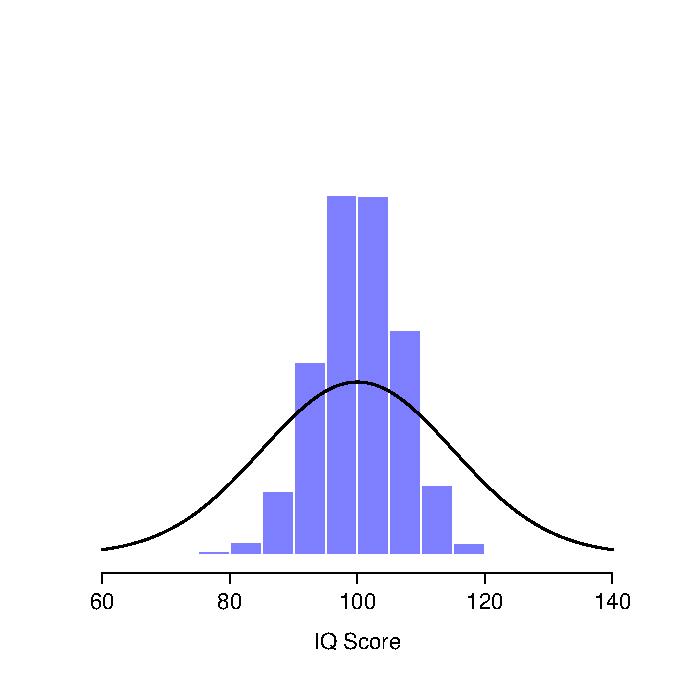
\includegraphics[width=9.38in]{/Users/dave/Documents/GitHub/stats-remix-advanced/img/estimation/sampleDist4} \caption{The sampling distribution of the mean for the "five IQ scores experiment". If you sample 5 people at random and calculate their *average* IQ, you'll almost certainly get a number between 80 and 120, even though there are quite a lot of individuals who have IQs above 120 or below 80. For comparison, the black line plots the population distribution of IQ scores.}\label{fig:sampdistmean}
\end{figure}

\begin{figure}
\includegraphics[width=9.38in]{/Users/dave/Documents/GitHub/stats-remix-advanced/img/estimation/sampleDistMax} \caption{The sampling distribution of the *maximum* for the "five IQ scores experiment". If you sample 5 people at random and select the one with the highest IQ score, you'll probably see someone with an IQ between 100 and 140.}\label{fig:sampdistmax}
\end{figure}

With an explanation of sampling distributions out of the way, Dave will now explain some additional detail behind this important concept.

\hypertarget{sample-size-and-population-size}{%
\subsection{Sample size and population size}\label{sample-size-and-population-size}}

Text by David Schuster

The size of a distribution is the number of units it contains. In mathematics, sample size is typically represented as \(n\) and population size is typically represented as \(N\). In APA-style writing, however, sample size is represented as \(N\), and \(n\) is used to represent a subsample (a part of a sample, such as the units in one condition). There does not seem to be a recommended symbol for population size in APA style. Why not? Many times, the population size is unknown.

\hypertarget{sampling-error}{%
\subsection{Sampling error}\label{sampling-error}}

Text by David Schuster

Sampling error is the mismatch between a sample statistic and a population parameter. As we have seen, taking a single random sample does not guarantee perfect representation of a population. Let's generate a population distribution, take a single random sample, and then compare the population and sample distributions:

\begin{Shaded}
\begin{Highlighting}[]
\NormalTok{population }\OtherTok{\textless{}{-}} \FunctionTok{runif}\NormalTok{(}\DecValTok{1000}\NormalTok{, }\DecValTok{1}\NormalTok{, }\DecValTok{100}\NormalTok{) }\CommentTok{\# Generate a variable called \textquotesingle{}population\textquotesingle{} with 1000 values chosen at random between 1 and 100}
\FunctionTok{mean}\NormalTok{(population) }\CommentTok{\# Display the mean of the population distribution}
\DocumentationTok{\#\# [1] 51.03521}
\FunctionTok{hist}\NormalTok{(population) }\CommentTok{\# Display a histogram of the population distribution}
\end{Highlighting}
\end{Shaded}

\includegraphics{schuster-statistics-remix_files/figure-latex/unnamed-chunk-240-1.pdf}

\begin{Shaded}
\begin{Highlighting}[]
\NormalTok{onesample }\OtherTok{\textless{}{-}} \FunctionTok{sample}\NormalTok{(population, }\AttributeTok{size =} \DecValTok{3}\NormalTok{, }\AttributeTok{replace =} \ConstantTok{TRUE}\NormalTok{) }\CommentTok{\# Take a random sample of size 3 from the population distribution with replacement}
\FunctionTok{mean}\NormalTok{(onesample) }\CommentTok{\# Display the mean of the sample distribution}
\DocumentationTok{\#\# [1] 63.59683}
\FunctionTok{hist}\NormalTok{(onesample) }\CommentTok{\# Display a histogram of the sample distribution}
\end{Highlighting}
\end{Shaded}

\includegraphics{schuster-statistics-remix_files/figure-latex/unnamed-chunk-240-2.pdf}

\begin{Shaded}
\begin{Highlighting}[]
\FunctionTok{mean}\NormalTok{(onesample) }\SpecialCharTok{{-}} \FunctionTok{mean}\NormalTok{(population) }\CommentTok{\# The difference between the sample mean and the population mean}
\DocumentationTok{\#\# [1] 12.56162}
\end{Highlighting}
\end{Shaded}

This required a few R functions you may not have seen before. \texttt{runif()} randomly generates uniform distributions (all values have equal probability) of any specified size and between any specified values. \texttt{sample()} takes a random sample from a specified distribution.

What was the difference between the sample mean and the population mean? If random sampling was perfect, it would be zero. Although these values were randomly generated, I am fairly confident the difference was not zero. Next, how do the \emph{shapes} of the two distributions compare?

Okay, the sample is not perfect. But sampling error is not dichotomous. Sometimes we can observe larger or smaller sampling error. What causes sampling error to be larger or smaller? First, we'll change \emph{sample size}:

\begin{Shaded}
\begin{Highlighting}[]
\NormalTok{population }\OtherTok{\textless{}{-}} \FunctionTok{runif}\NormalTok{(}\DecValTok{1000}\NormalTok{, }\DecValTok{1}\NormalTok{, }\DecValTok{100}\NormalTok{) }\CommentTok{\# Generate a variable called \textquotesingle{}population\textquotesingle{} with 1000 values chosen at random between 1 and 100}
\FunctionTok{mean}\NormalTok{(population) }\CommentTok{\# Display the mean of the population distribution}
\DocumentationTok{\#\# [1] 49.86771}
\FunctionTok{hist}\NormalTok{(population) }\CommentTok{\# Display a histogram of the population distribution}
\end{Highlighting}
\end{Shaded}

\includegraphics{schuster-statistics-remix_files/figure-latex/unnamed-chunk-241-1.pdf}

\begin{Shaded}
\begin{Highlighting}[]
\NormalTok{onesample }\OtherTok{\textless{}{-}} \FunctionTok{sample}\NormalTok{(population, }\AttributeTok{size =} \DecValTok{900}\NormalTok{, }\AttributeTok{replace =} \ConstantTok{TRUE}\NormalTok{) }\CommentTok{\# Take a random sample of size 900 from the population distribution with replacement}
\FunctionTok{mean}\NormalTok{(onesample) }\CommentTok{\# Display the mean of the sample distribution}
\DocumentationTok{\#\# [1] 48.71041}
\FunctionTok{hist}\NormalTok{(onesample) }\CommentTok{\# Display a histogram of the sample distribution}
\end{Highlighting}
\end{Shaded}

\includegraphics{schuster-statistics-remix_files/figure-latex/unnamed-chunk-241-2.pdf}

\begin{Shaded}
\begin{Highlighting}[]
\FunctionTok{mean}\NormalTok{(onesample) }\SpecialCharTok{{-}} \FunctionTok{mean}\NormalTok{(population) }\CommentTok{\# The difference between the sample mean and the population mean}
\DocumentationTok{\#\# [1] {-}1.157302}
\end{Highlighting}
\end{Shaded}

Did increasing the sample size to 900 increase or decrease sampling error? It decreased it. That hints that using a larger sample size can give us less sampling error. What do you think would happen if we put sample size back to 3 and, instead, changed the population so that all values were between 1 and 2?

Samples have variability because populations have variability; the sample mean ultimately depends on who gets selected to be in the sample. The larger the sample, the smaller the sampling error. The greater the variability in the population, the larger the sampling error.

Next, we will expand this discussion to consider what would happen if we construct a sampling distribution. We will take one sample, then take another and another. Our units will be sample means instead of scores.

\hypertarget{another-sampling-distribution}{%
\subsection{Another sampling distribution}\label{another-sampling-distribution}}

Text by David Schuster

A \textbf{sampling distribution} is a distribution of sample means.

If you take repeated samples, you can plot the mean of each sample. A collection of sample means forms a sampling distribution of the mean. Sampling distributions are made of many samples.

We will modify our prior example slightly. This time, we will create a loop (technically, a for\ldots next loop where we tell R how many times we want a command repeated) to repeat taking the sample mean. Loops are common in computer programming languages, but we don't use them very often when we do statistics in R. All you really need to know is that the loop causes the computer to repeat the commands inside the brackets.

\begin{Shaded}
\begin{Highlighting}[]
\NormalTok{population }\OtherTok{\textless{}{-}} \FunctionTok{runif}\NormalTok{(}\DecValTok{1000}\NormalTok{, }\DecValTok{1}\NormalTok{, }\DecValTok{100}\NormalTok{) }\CommentTok{\# Generate a variable called \textquotesingle{}population\textquotesingle{} with 1000 values chosen at random between 1 and 100}
\FunctionTok{mean}\NormalTok{(population) }\CommentTok{\# Display the mean of the population distribution}
\DocumentationTok{\#\# [1] 50.43223}
\FunctionTok{hist}\NormalTok{(population) }\CommentTok{\# Display a histogram of the population distribution}
\end{Highlighting}
\end{Shaded}

\includegraphics{schuster-statistics-remix_files/figure-latex/unnamed-chunk-242-1.pdf}

\begin{Shaded}
\begin{Highlighting}[]
\NormalTok{sampling }\OtherTok{=} \FunctionTok{rep}\NormalTok{(}\ConstantTok{NA}\NormalTok{, }\DecValTok{2000}\NormalTok{) }\CommentTok{\# create a variable with 2000 values of NA}
\ControlFlowTok{for}\NormalTok{(i }\ControlFlowTok{in} \DecValTok{1}\SpecialCharTok{:}\DecValTok{2000}\NormalTok{)\{}
\NormalTok{  onesample }\OtherTok{\textless{}{-}} \FunctionTok{sample}\NormalTok{(population, }\AttributeTok{size =} \DecValTok{5}\NormalTok{, }\AttributeTok{replace =} \ConstantTok{TRUE}\NormalTok{) }\CommentTok{\# take a random sample of size 5 from the population distribution with replacement  }
\NormalTok{  sampling[i] }\OtherTok{=} \FunctionTok{mean}\NormalTok{(onesample) }\CommentTok{\# add the sample\textquotesingle{}s mean to the sampling distribution}
\NormalTok{\}}
\FunctionTok{mean}\NormalTok{(sampling) }\CommentTok{\# Display the mean of the SAMPLING distribution}
\DocumentationTok{\#\# [1] 50.43477}
\FunctionTok{hist}\NormalTok{(sampling) }\CommentTok{\# Display a histogram of the SAMPLING distribution}
\end{Highlighting}
\end{Shaded}

\includegraphics{schuster-statistics-remix_files/figure-latex/unnamed-chunk-242-2.pdf}

\begin{Shaded}
\begin{Highlighting}[]
\FunctionTok{mean}\NormalTok{(sampling) }\SpecialCharTok{{-}} \FunctionTok{mean}\NormalTok{(population) }\CommentTok{\# The difference between the SAMPLING distribution mean and the population mean}
\DocumentationTok{\#\# [1] 0.002541854}
\end{Highlighting}
\end{Shaded}

Okay, some \emph{really} interesting things happened in this last example. Before we continue, make sure you understand the steps what we've taken to create a sampling distribution:

\begin{enumerate}
\def\labelenumi{\arabic{enumi}.}
\tightlist
\item
  We started with a population distribution. The shape of the population distribution is not important (did you notice that all the populations were close to a uniform distribution? None of the populations were normally distributed). While we're at it, the population \emph{size} is also not important. This example would have worked with a population of 50 or a population of 300,000.
\item
  We took a random sample from the population, with replacement. We found the mean of our random sample. We stored the mean in a variable called sampling.
\item
  We repeated Step 2 many times. Following this, we had a list of 2000 sample means stored in a variable called sampling. This is our sampling distribution. \textbf{Sampling distributions are made of sample means}. Put another way, the units of a sampling distribution are sample means.
\end{enumerate}

What did you you notice when you look at the histogram of the sampling distribution? It's normally distributed! We started with a non-normal population and ended up with a normally distributed sampling distribution. This is one of the outcomes specified by the central limit theorem.

What did you notice about the difference between the mean of the sampling distribution and the mean of the population? It's small. It is probably the smallest value of all the examples in this section. This is another outcome specified by the central limit theorem. As we collect more and more sample means, the mean of the sampling distribution will approach the mean of the population.

It has taken us a lot of steps and several examples to get here.

\hypertarget{defining-the-central-limit-theorem}{%
\subsection{Defining the central limit theorem}\label{defining-the-central-limit-theorem}}

Text by David Schuster

The central limit theorem (CLT) says that sampling distributions have special properties.

The CLT says that: (1) assuming two things, (2) if you do a series of steps, then (3) you will obtain an outcome. The outcome has implications for us.

\begin{itemize}
\tightlist
\item
  The two \textbf{assumptions} are a random sample and a variable that is continuous.
\item
  The \textbf{steps} are to take repeated random samples of the population and calculate the mean of each of those samples. Construct a sampling distribution from the sample means.
\item
  The \textbf{outcome} is that the histogram of the sample means is normally distributed. We call this the sampling distribution of the mean. It will always be normally distributed under the CLT, as long as we have a sufficiently large sample size.
\item
  This frequency distribution, like all frequency distributions, has a standard deviation called the standard error of the mean.
\end{itemize}

\hypertarget{more-on-standard-error}{%
\subsection{More on standard error}\label{more-on-standard-error}}

Text by David Schuster

Sampling distributions have a mean and standard deviation, just like any other distribution we have seen. However, the standard deviation of a sampling distribution has a special name: the standard error.

Standard error is calculated using this formula: \(\sigma_{\bar{X}}=\frac{\sigma}{\sqrt{n}}\)

In words: divide the standard deviation of the population by the square root of the sample size. Let's run the example one more time, this time calculating the standard error two ways:

\begin{Shaded}
\begin{Highlighting}[]
\NormalTok{population }\OtherTok{\textless{}{-}} \FunctionTok{runif}\NormalTok{(}\DecValTok{1000}\NormalTok{, }\DecValTok{1}\NormalTok{, }\DecValTok{100}\NormalTok{) }\CommentTok{\# Generate a variable called \textquotesingle{}population\textquotesingle{} with 1000 values chosen at random between 1 and 100}

\NormalTok{sampling }\OtherTok{=} \FunctionTok{rep}\NormalTok{(}\ConstantTok{NA}\NormalTok{, }\DecValTok{2000}\NormalTok{) }\CommentTok{\# create a variable with 2000 values of NA to store our sampling distribution}
\ControlFlowTok{for}\NormalTok{(i }\ControlFlowTok{in} \DecValTok{1}\SpecialCharTok{:}\DecValTok{2000}\NormalTok{)\{}
\NormalTok{  onesample }\OtherTok{\textless{}{-}} \FunctionTok{sample}\NormalTok{(population, }\AttributeTok{size =} \DecValTok{5}\NormalTok{, }\AttributeTok{replace =} \ConstantTok{TRUE}\NormalTok{) }\CommentTok{\# take a random sample of size 5 from the population distribution with replacement  }
\NormalTok{  sampling[i] }\OtherTok{=} \FunctionTok{mean}\NormalTok{(onesample) }\CommentTok{\# add the sample\textquotesingle{}s mean to the sampling distribution}
\NormalTok{\}}
\NormalTok{sampling\_sd }\OtherTok{\textless{}{-}} \FunctionTok{sqrt}\NormalTok{(}\FunctionTok{var}\NormalTok{(sampling) }\SpecialCharTok{*}\NormalTok{ (}\FunctionTok{length}\NormalTok{(sampling)}\SpecialCharTok{{-}}\DecValTok{1}\NormalTok{)}\SpecialCharTok{/}\FunctionTok{length}\NormalTok{(sampling)) }\CommentTok{\# Calculate the standard deviation of our observed (generated) sampling distribution}
\NormalTok{sampling\_sd }\CommentTok{\# Display the standard deviation of our observed (generated) sampling distribution}
\end{Highlighting}
\end{Shaded}

\begin{verbatim}
## [1] 12.63496
\end{verbatim}

\begin{Shaded}
\begin{Highlighting}[]
\NormalTok{pop\_sd }\OtherTok{\textless{}{-}} \FunctionTok{sqrt}\NormalTok{(}\FunctionTok{var}\NormalTok{(population) }\SpecialCharTok{*}\NormalTok{ (}\FunctionTok{length}\NormalTok{(population)}\SpecialCharTok{{-}}\DecValTok{1}\NormalTok{)}\SpecialCharTok{/}\FunctionTok{length}\NormalTok{(population)) }\CommentTok{\# find population standard deviation (the var() function gives sample variance and this converts it into population standard deviation)}
\NormalTok{standard\_error }\OtherTok{\textless{}{-}}\NormalTok{ pop\_sd }\SpecialCharTok{/} \FunctionTok{sqrt}\NormalTok{(}\DecValTok{5}\NormalTok{) }\CommentTok{\# Use the central limit theorem to calculate standard error using the formula}
\FunctionTok{print}\NormalTok{(standard\_error) }\CommentTok{\# Display the standard error}
\end{Highlighting}
\end{Shaded}

\begin{verbatim}
## [1] 12.65122
\end{verbatim}

\begin{Shaded}
\begin{Highlighting}[]
\NormalTok{standard\_error }\SpecialCharTok{{-}}\NormalTok{ sampling\_sd }\CommentTok{\# Display the difference between the calculated standard error and our observed standard deviation}
\end{Highlighting}
\end{Shaded}

\begin{verbatim}
## [1] 0.01626217
\end{verbatim}

They are pretty close. Why do we need the standard error formula if we could just find the standard deviation of the sampling distribution? Well, we typically do not work with the sampling distribution directly. We simply understand that it exists. Creating a sampling distribution requires the population distribution to be available to us, and this isn't usually the case when we are doing research. Further, the central limit theorem specifies taking an \emph{unlimited} number of samples in order for the sampling distribution mean to equal the population mean. It also requires a sample size of \(N\ge30\) when the population is not normally distributed. We have violated that rule (we used a uniform population distribution and we set our sample size as low as 5), but the numbers still came out pretty close.

Notice that if we assume that the central limit theorem applies, we already know the shape, mean, and standard deviation of a sampling distribution without having to construct it. This is one key to inferential statistics, and, specifically, \textbf{parametric statistics}. Parametric statistics that are methods that are based on known (or assumed) probability distributions. The sampling distribution of the mean is one such example.

\hypertarget{the-sampling-distribution-tells-us-about-the-probability-of-sample-means}{%
\subsection{The sampling distribution tells us about the probability of sample means}\label{the-sampling-distribution-tells-us-about-the-probability-of-sample-means}}

Where this gets useful is using the sampling distribution to make statements about the probability of obtaining a single sample mean. In many research contexts, we work with a single sample distribution. We do not have access to the population distribution nor the sampling distribution. But, we can use the central limit theorem to imagine what the sampling distribution looks like (it's normal with it's mean equal to the population mean and a standard error based on population standard deviation and sample size). Because the sampling distribution is made of sample means, it tells us about what we can expect if we take one single random sample from a population.

To summarize, the central limit theorem allows us to say useful things for research:

\begin{itemize}
\item
  A single random sample will have a mean that approximates the population mean. We can use samples in place of having to measure every member of the population.
\item
  Each time we take a random sample and calculate the mean, we are most likely to get the population mean.
\item
  Our sample means will vary. We can predict how much they vary by calculating the standard error.
\item
  It is possible to take a random sample and calculate the mean only to get a sample mean that is far away from the population mean, but this is unlikely to happen.
\item
  A larger sample size reduces the standard error of the mean. Larger sample sizes give us better estimates of the mean.
\end{itemize}

\hypertarget{sampling-distributions-exist-for-any-sample-statistic}{%
\subsection{Sampling distributions exist for any sample statistic!}\label{sampling-distributions-exist-for-any-sample-statistic}}

Text by \citet{Navarro2018}

One thing to keep in mind when thinking about sampling distributions is that \emph{any} sample statistic you might care to calculate has a sampling distribution. For example, suppose that each time I replicated the ``five IQ scores'' experiment I wrote down the largest IQ score in the experiment. This would give me a data set that started out like this:

\begin{verbatim}
                      110 117 122 119 113 ... 
\end{verbatim}

Doing this over and over again would give me a very different sampling distribution, namely the \emph{sampling distribution of the maximum}. The sampling distribution of the maximum of 5 IQ scores is shown in Figure \ref{fig:sampdistmax}. Not surprisingly, if you pick 5 people at random and then find the person with the highest IQ score, they're going to have an above average IQ. Most of the time you'll end up with someone whose IQ is measured in the 100 to 140 range.

\hypertarget{clt}{%
\subsection{The central limit theorem}\label{clt}}

An illustration of the how sampling distribution of the mean depends on sample size. In each panel, I generated 10,000 samples of IQ data, and calculated the mean IQ observed within each of these data sets. The histograms in these plots show the distribution of these means (i.e., the sampling distribution of the mean). Each individual IQ score was drawn from a normal distribution with mean 100 and standard deviation 15, which is shown as the solid black line).

\begin{figure}
\centering
\includegraphics{schuster-statistics-remix_files/figure-latex/IQsampa-1.pdf}
\caption{\label{fig:IQsampa}Each data set contained only a single observation, so the mean of each sample is just one person's IQ score. As a consequence, the sampling distribution of the mean is of course identical to the population distribution of IQ scores.}
\end{figure}

\begin{figure}
\centering
\includegraphics{schuster-statistics-remix_files/figure-latex/IQsampb-1.pdf}
\caption{\label{fig:IQsampb}When we raise the sample size to 2, the mean of any one sample tends to be closer to the population mean than a one person's IQ score, and so the histogram (i.e., the sampling distribution) is a bit narrower than the population distribution.}
\end{figure}

\begin{figure}
\centering
\includegraphics{schuster-statistics-remix_files/figure-latex/IQsampc-1.pdf}
\caption{\label{fig:IQsampc}By the time we raise the sample size to 10, we can see that the distribution of sample means tend to be fairly tightly clustered around the true population mean.}
\end{figure}

At this point I hope you have a pretty good sense of what sampling distributions are, and in particular what the sampling distribution of the mean is. In this section I want to talk about how the sampling distribution of the mean changes as a function of sample size. Intuitively, you already know part of the answer: if you only have a few observations, the sample mean is likely to be quite inaccurate: if you replicate a small experiment and recalculate the mean you'll get a very different answer. In other words, the sampling distribution is quite wide. If you replicate a large experiment and recalculate the sample mean you'll probably get the same answer you got last time, so the sampling distribution will be very narrow. You can see this visually in Figures \ref{fig:IQsampa}, \ref{fig:IQsampb} and \ref{fig:IQsampc}: the bigger the sample size, the narrower the sampling distribution gets. We can quantify this effect by calculating the standard deviation of the sampling distribution, which is referred to as the \textbf{\emph{standard error}}. The standard error of a statistic is often denoted SE, and since we're usually interested in the standard error of the sample \emph{mean}, we often use the acronym SEM. As you can see just by looking at the picture, as the sample size \(N\) increases, the SEM decreases.

Okay, so that's one part of the story. However, there's something I've been glossing over so far. All my examples up to this point have been based on the ``IQ scores'' experiments, and because IQ scores are roughly normally distributed, I've assumed that the population distribution is normal. What if it isn't normal? What happens to the sampling distribution of the mean? The remarkable thing is this: no matter what shape your population distribution is, as \(N\) increases the sampling distribution of the mean starts to look more like a normal distribution. To give you a sense of this, I ran some simulations using R. To do this, I started with the ``ramped'' distribution shown in the histogram in Figure \ref{fig:cltdemo}. As you can see by comparing the triangular shaped histogram to the bell curve plotted by the black line, the population distribution doesn't look very much like a normal distribution at all. Next, I used R to simulate the results of a large number of experiments. In each experiment I took \(N=2\) samples from this distribution, and then calculated the sample mean. Figure \ref{fig:cltdemo} plots the histogram of these sample means (i.e., the sampling distribution of the mean for \(N=2\)). This time, the histogram produces a \(\cap\)-shaped distribution: it's still not normal, but it's a lot closer to the black line than the population distribution in Figure \ref{fig:cltdemo}. When I increase the sample size to \(N=4\), the sampling distribution of the mean is very close to normal (Figure \ref{fig:cltdemo}, and by the time we reach a sample size of \(N=8\) it's almost perfectly normal. In other words, as long as your sample size isn't tiny, the sampling distribution of the mean will be approximately normal no matter what your population distribution looks like!

\begin{Shaded}
\begin{Highlighting}[]
    \CommentTok{\# needed for printing}
\NormalTok{    width }\OtherTok{\textless{}{-}} \DecValTok{6}
\NormalTok{    height }\OtherTok{\textless{}{-}} \DecValTok{6} 
    
    \CommentTok{\# parameters of the beta}
\NormalTok{    a }\OtherTok{\textless{}{-}} \DecValTok{2}
\NormalTok{    b }\OtherTok{\textless{}{-}} \DecValTok{1}
    
    \CommentTok{\# mean and standard deviation of the beta}
\NormalTok{    s }\OtherTok{\textless{}{-}} \FunctionTok{sqrt}\NormalTok{( a}\SpecialCharTok{*}\NormalTok{b }\SpecialCharTok{/}\NormalTok{ (a}\SpecialCharTok{+}\NormalTok{b)}\SpecialCharTok{\^{}}\DecValTok{2} \SpecialCharTok{/}\NormalTok{ (a}\SpecialCharTok{+}\NormalTok{b}\SpecialCharTok{+}\DecValTok{1}\NormalTok{) )}
\NormalTok{    m }\OtherTok{\textless{}{-}}\NormalTok{ a }\SpecialCharTok{/}\NormalTok{ (a}\SpecialCharTok{+}\NormalTok{b)}
    
    \CommentTok{\# define function to draw a plot}
\NormalTok{    plotOne }\OtherTok{\textless{}{-}} \ControlFlowTok{function}\NormalTok{(n,}\AttributeTok{N=}\DecValTok{50000}\NormalTok{) \{}
        
        \CommentTok{\# generate N random sample means of size n}
\NormalTok{        X }\OtherTok{\textless{}{-}} \FunctionTok{matrix}\NormalTok{(}\FunctionTok{rbeta}\NormalTok{(n}\SpecialCharTok{*}\NormalTok{N,a,b),n,N)}
\NormalTok{        X }\OtherTok{\textless{}{-}} \FunctionTok{colMeans}\NormalTok{(X)}
        
        \CommentTok{\# plot the data}
        \FunctionTok{hist}\NormalTok{( X, }\AttributeTok{breaks=}\FunctionTok{seq}\NormalTok{(}\DecValTok{0}\NormalTok{,}\DecValTok{1}\NormalTok{,.}\DecValTok{025}\NormalTok{), }\AttributeTok{border=}\StringTok{"white"}\NormalTok{, }\AttributeTok{freq=}\ConstantTok{FALSE}\NormalTok{,}
            \AttributeTok{col=}\FunctionTok{ifelse}\NormalTok{(colour,emphColLight,emphGrey),}
            \AttributeTok{xlab=}\StringTok{"Sample Mean"}\NormalTok{, }\AttributeTok{ylab=}\StringTok{""}\NormalTok{, }\AttributeTok{xlim=}\FunctionTok{c}\NormalTok{(}\DecValTok{0}\NormalTok{,}\FloatTok{1.2}\NormalTok{),}
            \AttributeTok{main=}\FunctionTok{paste}\NormalTok{(}\StringTok{"Sample Size ="}\NormalTok{,n), }\AttributeTok{axes=}\ConstantTok{FALSE}\NormalTok{,}
            \AttributeTok{font.main=}\DecValTok{1}\NormalTok{, }\AttributeTok{ylim=}\FunctionTok{c}\NormalTok{(}\DecValTok{0}\NormalTok{,}\DecValTok{5}\NormalTok{)}
\NormalTok{        )}
        \FunctionTok{box}\NormalTok{()}
        \FunctionTok{axis}\NormalTok{(}\DecValTok{1}\NormalTok{)}
        \CommentTok{\#axis(2)}
        
        \CommentTok{\# plot the theoretical distribution}
        \FunctionTok{lines}\NormalTok{( x }\OtherTok{\textless{}{-}} \FunctionTok{seq}\NormalTok{(}\DecValTok{0}\NormalTok{,}\FloatTok{1.2}\NormalTok{,.}\DecValTok{01}\NormalTok{), }\FunctionTok{dnorm}\NormalTok{(x,m,s}\SpecialCharTok{/}\FunctionTok{sqrt}\NormalTok{(n)), }
            \AttributeTok{lwd=}\DecValTok{2}\NormalTok{, }\AttributeTok{col=}\StringTok{"black"}\NormalTok{, }\AttributeTok{type=}\StringTok{"l"}
\NormalTok{        )}
\NormalTok{    \}}
    
    \ControlFlowTok{for}\NormalTok{( i }\ControlFlowTok{in} \FunctionTok{c}\NormalTok{(}\DecValTok{1}\NormalTok{,}\DecValTok{2}\NormalTok{,}\DecValTok{4}\NormalTok{,}\DecValTok{8}\NormalTok{)) \{}
        \FunctionTok{plotOne}\NormalTok{(i)\}}
\end{Highlighting}
\end{Shaded}

\includegraphics{schuster-statistics-remix_files/figure-latex/cltdemo-1.pdf} \includegraphics{schuster-statistics-remix_files/figure-latex/cltdemo-2.pdf} \includegraphics{schuster-statistics-remix_files/figure-latex/cltdemo-3.pdf} \includegraphics{schuster-statistics-remix_files/figure-latex/cltdemo-4.pdf}

On the basis of these figures, it seems like we have evidence for all of the following claims about the sampling distribution of the mean:

\begin{itemize}
\tightlist
\item
  The mean of the sampling distribution is the same as the mean of the population
\item
  The standard deviation of the sampling distribution (i.e., the standard error) gets smaller as the sample size increases
\item
  The shape of the sampling distribution becomes normal as the sample size increases
\end{itemize}

As it happens, not only are all of these statements true, there is a very famous theorem in statistics that proves all three of them, known as the \textbf{\emph{central limit theorem}}. Among other things, the central limit theorem tells us that if the population distribution has mean \(\mu\) and standard deviation \(\sigma\), then the sampling distribution of the mean also has mean \(\mu\), and the standard error of the mean is
\[
\mbox{SEM} = \frac{\sigma}{ \sqrt{N} }
\]
Because we divide the population standard devation \(\sigma\) by the square root of the sample size \(N\), the SEM gets smaller as the sample size increases. It also tells us that the shape of the sampling distribution becomes normal.\footnote{As usual, I'm being a bit sloppy here. The central limit theorem is a bit more general than this section implies. Like most introductory stats texts, I've discussed one situation where the central limit theorem holds: when you're taking an average across lots of independent events drawn from the same distribution. However, the central limit theorem is much broader than this. There's a whole class of things called ``\(U\)-statistics'' for instance, all of which satisfy the central limit theorem and therefore become normally distributed for large sample sizes. The mean is one such statistic, but it's not the only one.}

This result is useful for all sorts of things. It tells us why large experiments are more reliable than small ones, and because it gives us an explicit formula for the standard error it tells us \emph{how much} more reliable a large experiment is. It tells us why the normal distribution is, well, \emph{normal}. In real experiments, many of the things that we want to measure are actually averages of lots of different quantities (e.g., arguably, ``general'' intelligence as measured by IQ is an average of a large number of ``specific'' skills and abilities), and when that happens, the averaged quantity should follow a normal distribution. Because of this mathematical law, the normal distribution pops up over and over again in real data.

\hypertarget{pointestimates}{%
\section{Estimating population parameters}\label{pointestimates}}

Text by \citet{Navarro2018}

In all the IQ examples in the previous sections, we actually knew the population parameters ahead of time. As every undergraduate gets taught in their very first lecture on the measurement of intelligence, IQ scores are \emph{defined} to have mean 100 and standard deviation 15. However, this is a bit of a lie. How do we know that IQ scores have a true population mean of 100? Well, we know this because the people who designed the tests have administered them to very large samples, and have then ``rigged'' the scoring rules so that their sample has mean 100. That's not a bad thing of course: it's an important part of designing a psychological measurement. However, it's important to keep in mind that this theoretical mean of 100 only attaches to the population that the test designers used to design the tests. Good test designers will actually go to some lengths to provide ``test norms'' that can apply to lots of different populations (e.g., different age groups, nationalities etc).

This is very handy, but of course almost every research project of interest involves looking at a different population of people to those used in the test norms. For instance, suppose you wanted to measure the effect of low level lead poisoning on cognitive functioning in Port Pirie, a South Australian industrial town with a lead smelter. Perhaps you decide that you want to compare IQ scores among people in Port Pirie to a comparable sample in Whyalla, a South Australian industrial town with a steel refinery.\footnote{Please note that if you were \emph{actually} interested in this question, you would need to be a \emph{lot} more careful than I'm being here. You \emph{can't} just compare IQ scores in Whyalla to Port Pirie and assume that any differences are due to lead poisoning. Even if it were true that the only differences between the two towns corresponded to the different refineries (and it isn't, not by a long shot), you need to account for the fact that people already \emph{believe} that lead pollution causes cognitive deficits: if you recall back to Chapter \ref{studydesign}, this means that there are different demand effects for the Port Pirie sample than for the Whyalla sample. In other words, you might end up with an illusory group difference in your data, caused by the fact that people \emph{think} that there is a real difference. I find it pretty implausible to think that the locals wouldn't be well aware of what you were trying to do if a bunch of researchers turned up in Port Pirie with lab coats and IQ tests, and even less plausible to think that a lot of people would be pretty resentful of you for doing it. Those people won't be as co-operative in the tests. Other people in Port Pirie might be \emph{more} motivated to do well because they don't want their home town to look bad. The motivational effects that would apply in Whyalla are likely to be weaker, because people don't have any concept of ``iron ore poisoning'' in the same way that they have a concept for ``lead poisoning''. Psychology is \emph{hard}.} Regardless of which town you're thinking about, it doesn't make a lot of sense simply to \emph{assume} that the true population mean IQ is 100. No-one has, to my knowledge, produced sensible norming data that can automatically be applied to South Australian industrial towns. We're going to have to \textbf{\emph{estimate}} the population parameters from a sample of data. So how do we do this?

\hypertarget{estimating-the-population-mean}{%
\subsection{Estimating the population mean}\label{estimating-the-population-mean}}

Suppose we go to Port Pirie and 100 of the locals are kind enough to sit through an IQ test. The average IQ score among these people turns out to be \(\bar{X}=98.5\). So what is the true mean IQ for the entire population of Port Pirie? Obviously, we don't know the answer to that question. It could be \(97.2\), but if could also be \(103.5\). Our sampling isn't exhaustive so we cannot give a definitive answer. Nevertheless if I was forced at gunpoint to give a ``best guess'' I'd have to say \(98.5\). That's the essence of statistical estimation: giving a best guess.

In this example, estimating the unknown poulation parameter is straightforward. I calculate the sample mean, and I use that as my \textbf{\emph{estimate of the population mean}}. It's pretty simple, and in the next section I'll explain the statistical justification for this intuitive answer. However, for the moment what I want to do is make sure you recognise that the sample statistic and the estimate of the population parameter are conceptually different things. A sample statistic is a description of your data, whereas the estimate is a guess about the population. With that in mind, statisticians often different notation to refer to them. For instance, if true population mean is denoted \(\mu\), then we would use \(\hat\mu\) to refer to our estimate of the population mean. In contrast, the sample mean is denoted \(\bar{X}\) or sometimes \(m\). However, in simple random samples, the estimate of the population mean is identical to the sample mean: if I observe a sample mean of \(\bar{X} = 98.5\), then my estimate of the population mean is also \(\hat\mu = 98.5\). To help keep the notation clear, here's a handy table:

\begin{Shaded}
\begin{Highlighting}[]
\NormalTok{knitr}\SpecialCharTok{::}\FunctionTok{kable}\NormalTok{(}\FunctionTok{data.frame}\NormalTok{(}\AttributeTok{stringsAsFactors=}\ConstantTok{FALSE}\NormalTok{,}
                   \AttributeTok{Symbol =} \FunctionTok{c}\NormalTok{(}\StringTok{"$}\SpecialCharTok{\textbackslash{}\textbackslash{}}\StringTok{bar\{X\}$"}\NormalTok{, }\StringTok{"$}\SpecialCharTok{\textbackslash{}\textbackslash{}}\StringTok{mu$"}\NormalTok{, }\StringTok{"$}\SpecialCharTok{\textbackslash{}\textbackslash{}}\StringTok{hat\{}\SpecialCharTok{\textbackslash{}\textbackslash{}}\StringTok{mu\}$"}\NormalTok{),}
              \AttributeTok{What.is.it =} \FunctionTok{c}\NormalTok{(}\StringTok{"Sample mean"}\NormalTok{, }\StringTok{"True population mean"}\NormalTok{,}
                              \StringTok{"Estimate of the population mean"}\NormalTok{),}
   \AttributeTok{Do.we.know.what.it.is =} \FunctionTok{c}\NormalTok{(}\StringTok{"Yes  calculated from the raw data"}\NormalTok{,}
                              \StringTok{"Almost never known for sure"}\NormalTok{,}
                              \StringTok{"Yes  identical to the sample mean"}\NormalTok{)))}
\end{Highlighting}
\end{Shaded}

\begin{tabular}{l|l|l}
\hline
Symbol & What.is.it & Do.we.know.what.it.is\\
\hline
\$\textbackslash{}bar\{X\}\$ & Sample mean & Yes  calculated from the raw data\\
\hline
\$\textbackslash{}mu\$ & True population mean & Almost never known for sure\\
\hline
\$\textbackslash{}hat\{\textbackslash{}mu\}\$ & Estimate of the population mean & Yes  identical to the sample mean\\
\hline
\end{tabular}

\hypertarget{estimating-the-population-standard-deviation}{%
\subsection{Estimating the population standard deviation}\label{estimating-the-population-standard-deviation}}

So far, estimation seems pretty simple, and you might be wondering why I forced you to read through all that stuff about sampling theory. In the case of the mean, our estimate of the population parameter (i.e.~\(\hat\mu\)) turned out to identical to the corresponding sample statistic (i.e.~\(\bar{X}\)). However, that's not always true. To see this, let's have a think about how to construct an \textbf{\emph{estimate of the population standard deviation}}, which we'll denote \(\hat\sigma\). What shall we use as our estimate in this case? Your first thought might be that we could do the same thing we did when estimating the mean, and just use the sample statistic as our estimate. That's almost the right thing to do, but not quite.

Here's why. Suppose I have a sample that contains a single observation. For this example, it helps to consider a sample where you have no intutions at all about what the true population values might be, so let's use something completely fictitious. Suppose the observation in question measures the \emph{cromulence} of my shoes. It turns out that my shoes have a cromulence of 20. So here's my sample:

\begin{verbatim}
20
\end{verbatim}

This is a perfectly legitimate sample, even if it does have a sample size of \(N=1\). It has a sample mean of 20, and because every observation in this sample is equal to the sample mean (obviously!) it has a sample standard deviation of 0. As a description of the \emph{sample} this seems quite right: the sample contains a single observation and therefore there is no variation observed within the sample. A sample standard deviation of \(s = 0\) is the right answer here. But as an estimate of the \emph{population} standard deviation, it feels completely insane, right? Admittedly, you and I don't know anything at all about what ``cromulence'' is, but we know something about data: the only reason that we don't see any variability in the \emph{sample} is that the sample is too small to display any variation! So, if you have a sample size of \(N=1\), it \emph{feels} like the right answer is just to say ``no idea at all''.

Notice that you \emph{don't} have the same intuition when it comes to the sample mean and the population mean. If forced to make a best guess about the population mean, it doesn't feel completely insane to guess that the population mean is 20. Sure, you probably wouldn't feel very confident in that guess, because you have only the one observation to work with, but it's still the best guess you can make.

Let's extend this example a little. Suppose I now make a second observation. My data set now has \(N=2\) observations of the cromulence of shoes, and the complete sample now looks like this:

\begin{verbatim}
20, 22
\end{verbatim}

This time around, our sample is \emph{just} large enough for us to be able to observe some variability: two observations is the bare minimum number needed for any variability to be observed! For our new data set, the sample mean is \(\bar{X}=21\), and the sample standard deviation is \(s=1\). What intuitions do we have about the population? Again, as far as the population mean goes, the best guess we can possibly make is the sample mean: if forced to guess, we'd probably guess that the population mean cromulence is 21. What about the standard deviation? This is a little more complicated. The sample standard deviation is only based on two observations, and if you're at all like me you probably have the intuition that, with only two observations, we haven't given the population ``enough of a chance'' to reveal its true variability to us. It's not just that we suspect that the estimate is \emph{wrong}: after all, with only two observations we expect it to be wrong to some degree. The worry is that the error is \emph{systematic}. Specifically, we suspect that the sample standard deviation is likely to be smaller than the population standard deviation.

\begin{figure}
\includegraphics[width=9.38in]{/Users/dave/Documents/GitHub/stats-remix-advanced/img/estimation/samplingDistSampleSD} \caption{The sampling distribution of the sample standard deviation for a "two IQ scores" experiment. The true population standard deviation is 15 (dashed line), but as you can see from the histogram, the vast majority of experiments will produce a much smaller sample standard deviation than this. On average, this experiment would produce a sample standard deviation of only 8.5, well below the true value! In other words, the sample standard deviation is a *biased* estimate of the population standard deviation. }\label{fig:sampdistsd}
\end{figure}

This intuition feels right, but it would be nice to demonstrate this somehow. There are in fact mathematical proofs that confirm this intuition, but unless you have the right mathematical background they don't help very much. Instead, what I'll do is use R to simulate the results of some experiments. With that in mind, let's return to our IQ studies. Suppose the true population mean IQ is 100 and the standard deviation is 15. I can use the \texttt{rnorm()} function to generate the the results of an experiment in which I measure \(N=2\) IQ scores, and calculate the sample standard deviation. If I do this over and over again, and plot a histogram of these sample standard deviations, what I have is the \emph{sampling distribution of the standard deviation}. I've plotted this distribution in Figure \ref{fig:sampdistsd}. Even though the true population standard deviation is 15, the average of the \emph{sample} standard deviations is only 8.5. Notice that this is a very different result to what we found in Figure \ref{fig:IQsampb} when we plotted the sampling distribution of the mean. If you look at that sampling distribution, what you see is that the population mean is 100, and the average of the sample means is also 100.

Now let's extend the simulation. Instead of restricting ourselves to the situation where we have a sample size of \(N=2\), let's repeat the exercise for sample sizes from 1 to 10. If we plot the average sample mean and average sample standard deviation as a function of sample size, you get the results shown in Figure \ref{fig:estimatorbias}. On the left hand side (panel a), I've plotted the average sample mean and on the right hand side (panel b), I've plotted the average standard deviation. The two plots are quite different: \emph{on average}, the average sample mean is equal to the population mean. It is an \textbf{\emph{unbiased estimator}}, which is essentially the reason why your best estimate for the population mean is the sample mean.\footnote{I should note that I'm hiding something here. Unbiasedness is a desirable characteristic for an estimator, but there are other things that matter besides bias. However, it's beyond the scope of this book to discuss this in any detail. I just want to draw your attention to the fact that there's some hidden complexity here.} The plot on the right is quite different: on average, the sample standard deviation \(s\) is \emph{smaller} than the population standard deviation \(\sigma\). It is a \textbf{\emph{biased estimator}}. In other words, if we want to make a ``best guess'' \(\hat\sigma\) about the value of the population standard deviation \(\sigma\), we should make sure our guess is a little bit larger than the sample standard deviation \(s\).

\begin{figure}
\includegraphics[width=8.35in]{/Users/dave/Documents/GitHub/stats-remix-advanced/img/estimation/biasMean} \caption{An illustration of the fact that the sample mean is an unbiased estimator of the population mean (panel a), but the sample standard deviation is a biased estimator of the population standard deviation (panel b). To generate the figure, I generated 10,000 simulated data sets with 1 observation each, 10,000 more with 2 observations, and so on up to a sample size of 10. Each data set consisted of fake IQ data: that is, the data were normally distributed with a true population mean of 100 and standard deviation 15. *On average*, the sample means turn out to be 100, regardless of sample size (panel a). However, the sample standard deviations turn out to be systematically too small (panel b), especially for small sample sizes.}\label{fig:estimatorbias}
\end{figure}

The fix to this systematic bias turns out to be very simple. Here's how it works. Before tackling the standard deviation, let's look at the variance. If you recall from Section \ref{var}, the sample variance is defined to be the average of the squared deviations from the sample mean. That is:
\[
s^2 = \frac{1}{N} \sum_{i=1}^N (X_i - \bar{X})^2
\]
The sample variance \(s^2\) is a biased estimator of the population variance \(\sigma^2\). But as it turns out, we only need to make a tiny tweak to transform this into an unbiased estimator. All we have to do is divide by \(N-1\) rather than by \(N\). If we do that, we obtain the following formula:
\[
\hat\sigma^2 = \frac{1}{N-1} \sum_{i=1}^N (X_i - \bar{X})^2 
\]
This is an unbiased estimator of the population variance \(\sigma\). Moreover, this finally answers the question we raised in Section \ref{var}. Why did R give us slightly different answers when we used the \texttt{var()} function? Because the \texttt{var()} function calculates \(\hat\sigma^2\) not \(s^2\), that's why. A similar story applies for the standard deviation. If we divide by \(N-1\) rather than \(N\), our estimate of the population standard deviation becomes:
\[
\hat\sigma = \sqrt{\frac{1}{N-1} \sum_{i=1}^N (X_i - \bar{X})^2} 
\]
and when we use R's built in standard deviation function \texttt{sd()}, what it's doing is calculating \(\hat\sigma\), not \(s\).\footnote{Okay, I'm hiding something else here. In a bizarre and counterintuitive twist, since \(\hat\sigma^2\) is an unbiased estimator of \(\sigma^2\), you'd assume that taking the square root would be fine, and \(\hat\sigma\) would be an unbiased estimator of \(\sigma\). Right? Weirdly, it's not. There's actually a subtle, tiny bias in \(\hat\sigma\). This is just bizarre: \(\hat\sigma^2\) is and unbiased estimate of the population variance \(\sigma^2\), but when you take the square root, it turns out that \(\hat\sigma\) is a biased estimator of the population standard deviation \(\sigma\). Weird, weird, weird, right? So, why is \(\hat\sigma\) biased? The technical answer is ``because non-linear transformations (e.g., the square root) don't commute with expectation'', but that just sounds like gibberish to everyone who hasn't taken a course in mathematical statistics. Fortunately, it doesn't matter for practical purposes. The bias is small, and in real life everyone uses \(\hat\sigma\) and it works just fine. Sometimes mathematics is just annoying.}

One final point: in practice, a lot of people tend to refer to \(\hat{\sigma}\) (i.e., the formula where we divide by \(N-1\)) as the \emph{sample} standard deviation. Technically, this is incorrect: the \emph{sample} standard deviation should be equal to \(s\) (i.e., the formula where we divide by \(N\)). These aren't the same thing, either conceptually or numerically. One is a property of the sample, the other is an estimated characteristic of the population. However, in almost every real life application, what we actually care about is the estimate of the population parameter, and so people always report \(\hat\sigma\) rather than \(s\). This is the right number to report, of course, it's that people tend to get a little bit imprecise about terminology when they write it up, because ``sample standard deviation'' is shorter than ``estimated population standard deviation''. It's no big deal, and in practice I do the same thing everyone else does. Nevertheless, I think it's important to keep the two \emph{concepts} separate: it's never a good idea to confuse ``known properties of your sample'' with ``guesses about the population from which it came''. The moment you start thinking that \(s\) and \(\hat\sigma\) are the same thing, you start doing exactly that.

To finish this section off, here's another couple of tables to help keep things clear:

\begin{Shaded}
\begin{Highlighting}[]
\NormalTok{knitr}\SpecialCharTok{::}\FunctionTok{kable}\NormalTok{(}\FunctionTok{data.frame}\NormalTok{(}\AttributeTok{stringsAsFactors=}\ConstantTok{FALSE}\NormalTok{,}
                   \AttributeTok{Symbol =} \FunctionTok{c}\NormalTok{(}\StringTok{"$s$"}\NormalTok{, }\StringTok{"$}\SpecialCharTok{\textbackslash{}\textbackslash{}}\StringTok{sigma$"}\NormalTok{, }\StringTok{"$}\SpecialCharTok{\textbackslash{}\textbackslash{}}\StringTok{hat\{}\SpecialCharTok{\textbackslash{}\textbackslash{}}\StringTok{sigma\}$"}\NormalTok{, }\StringTok{"$s\^{}2$"}\NormalTok{,}
                              \StringTok{"$}\SpecialCharTok{\textbackslash{}\textbackslash{}}\StringTok{sigma\^{}2$"}\NormalTok{, }\StringTok{"$}\SpecialCharTok{\textbackslash{}\textbackslash{}}\StringTok{hat\{}\SpecialCharTok{\textbackslash{}\textbackslash{}}\StringTok{sigma\}\^{}2$"}\NormalTok{),}
              \AttributeTok{What.is.it =} \FunctionTok{c}\NormalTok{(}\StringTok{"Sample standard deviation"}\NormalTok{,}
                              \StringTok{"Population standard deviation"}\NormalTok{,}
                              \StringTok{"Estimate of the population standard deviation"}\NormalTok{, }\StringTok{"Sample variance"}\NormalTok{,}
                              \StringTok{"Population variance"}\NormalTok{,}
                              \StringTok{"Estimate of the population variance"}\NormalTok{),}
   \AttributeTok{Do.we.know.what.it.is =} \FunctionTok{c}\NormalTok{(}\StringTok{"Yes {-} calculated from the raw data"}\NormalTok{,}
                              \StringTok{"Almost never known for sure"}\NormalTok{,}
                              \StringTok{"Yes {-} but not the same as the sample standard deviation"}\NormalTok{,}
                              \StringTok{"Yes {-} calculated from the raw data"}\NormalTok{,}
                              \StringTok{"Almost never known for sure"}\NormalTok{,}
                              \StringTok{"Yes {-}  but not the same as the sample variance"}\NormalTok{)}
\NormalTok{))}
\end{Highlighting}
\end{Shaded}

\begin{tabular}{l|l|l}
\hline
Symbol & What.is.it & Do.we.know.what.it.is\\
\hline
\$s\$ & Sample standard deviation & Yes - calculated from the raw data\\
\hline
\$\textbackslash{}sigma\$ & Population standard deviation & Almost never known for sure\\
\hline
\$\textbackslash{}hat\{\textbackslash{}sigma\}\$ & Estimate of the population standard deviation & Yes - but not the same as the sample standard deviation\\
\hline
\$s\textasciicircum{}2\$ & Sample variance & Yes - calculated from the raw data\\
\hline
\$\textbackslash{}sigma\textasciicircum{}2\$ & Population variance & Almost never known for sure\\
\hline
\$\textbackslash{}hat\{\textbackslash{}sigma\}\textasciicircum{}2\$ & Estimate of the population variance & Yes -  but not the same as the sample variance\\
\hline
\end{tabular}

\hypertarget{ci}{%
\section{Estimating a confidence interval}\label{ci}}

Text by \citet{Navarro2018}

\begin{quote}
\emph{Statistics means never having to say you're certain} -- Unknown origin\footnote{This quote appears on a great many t-shirts and websites, and even gets a mention in a few academic papers (e.g., \textbackslash url\{\url{http://www.amstat.org/publications/jse/v10n3/friedman.html}} but I've never found the original source.
\end{quote}

Up to this point in this chapter, I've outlined the basics of sampling theory which statisticians rely on to make guesses about population parameters on the basis of a sample of data. As this discussion illustrates, one of the reasons we need all this sampling theory is that every data set leaves us with a some of uncertainty, so our estimates are never going to be perfectly accurate. The thing that has been missing from this discussion is an attempt to \emph{quantify} the amount of uncertainty that attaches to our estimate. It's not enough to be able guess that, say, the mean IQ of undergraduate psychology students is 115 (yes, I just made that number up). We also want to be able to say something that expresses the degree of certainty that we have in our guess. For example, it would be nice to be able to say that there is a 95\% chance that the true mean lies between 109 and 121. The name for this is a \textbf{\emph{confidence interval}} for the mean.

Armed with an understanding of sampling distributions, constructing a confidence interval for the mean is actually pretty easy. Here's how it works. Suppose the true population mean is \(\mu\) and the standard deviation is \(\sigma\). I've just finished running my study that has \(N\) participants, and the mean IQ among those participants is \(\bar{X}\). We know from our discussion of the central limit theorem (Section \ref{clt} that the sampling distribution of the mean is approximately normal. We also know from our discussion of the normal distribution Section \ref{normal} that there is a 95\% chance that a normally-distributed quantity will fall within two standard deviations of the true mean. To be more precise, we can use the \texttt{qnorm()} function to compute the 2.5th and 97.5th percentiles of the normal distribution

\begin{Shaded}
\begin{Highlighting}[]
\FunctionTok{qnorm}\NormalTok{( }\AttributeTok{p =} \FunctionTok{c}\NormalTok{(.}\DecValTok{025}\NormalTok{, .}\DecValTok{975}\NormalTok{) )}
\end{Highlighting}
\end{Shaded}

\begin{verbatim}
## [1] -1.959964  1.959964
\end{verbatim}

Okay, so I lied earlier on. The more correct answer is that 95\% chance that a normally-distributed quantity will fall within 1.96 standard deviations of the true mean. Next, recall that the standard deviation of the sampling distribution is referred to as the standard error, and the standard error of the mean is written as SEM. When we put all these pieces together, we learn that there is a 95\% probability that the sample mean \(\bar{X}\) that we have actually observed lies within 1.96 standard errors of the population mean. Mathematically, we write this as:
\[
\mu - \left( 1.96 \times \mbox{SEM} \right) \ \leq \  \bar{X}\  \leq \  \mu + \left( 1.96 \times \mbox{SEM} \right) 
\]
where the SEM is equal to \(\sigma / \sqrt{N}\), and we can be 95\% confident that this is true. However, that's not answering the question that we're actually interested in. The equation above tells us what we should expect about the sample mean, given that we know what the population parameters are. What we \emph{want} is to have this work the other way around: we want to know what we should believe about the population parameters, given that we have observed a particular sample. However, it's not too difficult to do this. Using a little high school algebra, a sneaky way to rewrite our equation is like this:
\[
\bar{X} -  \left( 1.96 \times \mbox{SEM} \right) \ \leq \ \mu  \ \leq  \ \bar{X} +  \left( 1.96 \times \mbox{SEM}\right)
\]
What this is telling is is that the range of values has a 95\% probability of containing the population mean \(\mu\). We refer to this range as a \textbf{\emph{95\% confidence interval}}, denoted \(\mbox{CI}_{95}\). In short, as long as \(N\) is sufficiently large -- large enough for us to believe that the sampling distribution of the mean is normal -- then we can write this as our formula for the 95\% confidence interval:
\[
\mbox{CI}_{95} = \bar{X} \pm \left( 1.96 \times \frac{\sigma}{\sqrt{N}} \right)
\]
Of course, there's nothing special about the number 1.96: it just happens to be the multiplier you need to use if you want a 95\% confidence interval. If I'd wanted a 70\% confidence interval, I could have used the \texttt{qnorm()} function to calculate the 15th and 85th quantiles:

\begin{Shaded}
\begin{Highlighting}[]
\FunctionTok{qnorm}\NormalTok{( }\AttributeTok{p =} \FunctionTok{c}\NormalTok{(.}\DecValTok{15}\NormalTok{, .}\DecValTok{85}\NormalTok{) )}
\end{Highlighting}
\end{Shaded}

\begin{verbatim}
## [1] -1.036433  1.036433
\end{verbatim}

and so the formula for \(\mbox{CI}_{70}\) would be the same as the formula for \(\mbox{CI}_{95}\) except that we'd use 1.04 as our magic number rather than 1.96.

\hypertarget{a-slight-mistake-in-the-formula}{%
\subsection{A slight mistake in the formula}\label{a-slight-mistake-in-the-formula}}

As usual, I lied. The formula that I've given above for the 95\% confidence interval is approximately correct, but I glossed over an important detail in the discussion. Notice my formula requires you to use the standard error of the mean, SEM, which in turn requires you to use the true population standard deviation \(\sigma\). Yet, in Section \ref{pointestimates} I stressed the fact that we don't actually \emph{know} the true population parameters. Because we don't know the true value of \(\sigma\), we have to use an estimate of the population standard deviation \(\hat{\sigma}\) instead. This is pretty straightforward to do, but this has the consequence that we need to use the quantiles of the \(t\)-distribution rather than the normal distribution to calculate our magic number; and the answer depends on the sample size. When \(N\) is very large, we get pretty much the same value using \texttt{qt()} that we would if we used \texttt{qnorm()}\ldots{}

\begin{Shaded}
\begin{Highlighting}[]
\NormalTok{N }\OtherTok{\textless{}{-}} \DecValTok{10000}   \CommentTok{\# suppose our sample size is 10,000}
\FunctionTok{qt}\NormalTok{( }\AttributeTok{p =}\NormalTok{ .}\DecValTok{975}\NormalTok{, }\AttributeTok{df =}\NormalTok{ N}\DecValTok{{-}1}\NormalTok{)   }\CommentTok{\# calculate the 97.5th quantile of the t{-}dist}
\end{Highlighting}
\end{Shaded}

\begin{verbatim}
## [1] 1.960201
\end{verbatim}

But when \(N\) is small, we get a much bigger number when we use the \(t\) distribution:

\begin{Shaded}
\begin{Highlighting}[]
\NormalTok{N }\OtherTok{\textless{}{-}} \DecValTok{10}   \CommentTok{\# suppose our sample size is 10}
\FunctionTok{qt}\NormalTok{( }\AttributeTok{p =}\NormalTok{ .}\DecValTok{975}\NormalTok{, }\AttributeTok{df =}\NormalTok{ N}\DecValTok{{-}1}\NormalTok{)   }\CommentTok{\# calculate the 97.5th quantile of the t{-}dist}
\end{Highlighting}
\end{Shaded}

\begin{verbatim}
## [1] 2.262157
\end{verbatim}

There's nothing too mysterious about what's happening here. Bigger values mean that the confidence interval is wider, indicating that we're more uncertain about what the true value of \(\mu\) actually is. When we use the \(t\) distribution instead of the normal distribution, we get bigger numbers, indicating that we have more uncertainty. And why do we have that extra uncertainty? Well, because our estimate of the population standard deviation \(\hat\sigma\) might be wrong! If it's wrong, it implies that we're a bit less sure about what our sampling distribution of the mean actually looks like\ldots{} and this uncertainty ends up getting reflected in a wider confidence interval.

\hypertarget{interpreting-a-confidence-interval}{%
\subsection{Interpreting a confidence interval}\label{interpreting-a-confidence-interval}}

The hardest thing about confidence intervals is understanding what they \emph{mean}. Whenever people first encounter confidence intervals, the first instinct is almost always to say that ``there is a 95\% probabaility that the true mean lies inside the confidence interval''. It's simple, and it seems to capture the common sense idea of what it means to say that I am ``95\% confident''. Unfortunately, it's not quite right. The intuitive definition relies very heavily on your own personal \emph{beliefs} about the value of the population mean. I say that I am 95\% confident because those are my beliefs. In everyday life that's perfectly okay, but if you remember back to Section \ref{probmeaning}, you'll notice that talking about personal belief and confidence is a Bayesian idea. Personally (speaking as a Bayesian) I have no problem with the idea that the phrase ``95\% probability'' is allowed to refer to a personal belief. However, confidence intervals are \emph{not} Bayesian tools. Like everything else in this chapter, confidence intervals are \emph{frequentist} tools, and if you are going to use frequentist methods then it's not appropriate to attach a Bayesian interpretation to them. If you use frequentist methods, you must adopt frequentist interpretations!

Okay, so if that's not the right answer, what is? Remember what we said about frequentist probability: the only way we are allowed to make ``probability statements'' is to talk about a sequence of events, and to count up the frequencies of different kinds of events. From that perspective, the interpretation of a 95\% confidence interval must have something to do with replication. Specifically: if we replicated the experiment over and over again and computed a 95\% confidence interval for each replication, then 95\% of those \emph{intervals} would contain the true mean. More generally, 95\% of all confidence intervals constructed using this procedure should contain the true population mean. This idea is illustrated in Figure \ref{fig:cirep}, which shows 50 confidence intervals constructed for a ``measure 10 IQ scores'' experiment (top panel) and another 50 confidence intervals for a ``measure 25 IQ scores'' experiment (bottom panel). A bit fortuitously, across the 100 replications that I simulated, it turned out that exactly 95 of them contained the true mean.

\textbackslash begin\{figure\}
\includegraphics[width=16.67in]{/Users/dave/Documents/GitHub/stats-remix-advanced/img/estimation/confIntReplicated} \textbackslash caption\{95\% confidence intervals. The top (panel a) shows 50 simulated replications of an experiment in which we measure the IQs of 10 people. The dot marks the location of the sample mean, and the line shows the 95\% confidence interval. In total 47 of the 50 confidence intervals do contain the true mean (i.e., 100), but the three intervals marked with asterisks do not. The lower graph (panel b) shows a similar simulation, but this time we simulate replications of an experiment that measures the IQs of 25 people.\}\label{fig:cirep}
\textbackslash end\{figure\}

The critical difference here is that the Bayesian claim makes a probability statement about the population mean (i.e., it refers to our uncertainty about the population mean), which is not allowed under the frequentist interpretation of probability because you can't ``replicate'' a population! In the frequentist claim, the population mean is fixed and no probabilistic claims can be made about it. Confidence intervals, however, are repeatable so we can replicate experiments. Therefore a frequentist is allowed to talk about the probability that the \emph{confidence interval} (a random variable) contains the true mean; but is not allowed to talk about the probability that the \emph{true population mean} (not a repeatable event) falls within the confidence interval.

I know that this seems a little pedantic, but it does matter. It matters because the difference in interpretation leads to a difference in the mathematics. There is a Bayesian alternative to confidence intervals, known as \emph{credible intervals}. In most situations credible intervals are quite similar to confidence intervals, but in other cases they are drastically different. As promised, though, I'll talk more about the Bayesian perspective in Chapter \ref{bayes}.

\hypertarget{calculating-confidence-intervals-in-r}{%
\subsection{Calculating confidence intervals in R}\label{calculating-confidence-intervals-in-r}}

As far as I can tell, the core packages in R don't include a simple function for calculating confidence intervals for the mean. They \emph{do} include a lot of complicated, extremely powerful functions that can be used to calculate confidence intervals associated with lots of different things, such as the \texttt{confint()} function that we'll use in Chapter \ref{regression}. But I figure that when you're first learning statistics, it might be useful to start with something simpler. As a consequence, the \texttt{lsr} package includes a function called \texttt{ciMean()} which you can use to calculate your confidence intervals. There are two arguments that you might want to specify:\footnote{As of the current writing, these are the only arguments to the function. However, I am planning to add a bit more functionality to \texttt{ciMean()}. However, regardless of what those future changes might look like, the \texttt{x} and \texttt{conf} arguments will remain the same, and the commands used in this book will still work.}

\begin{itemize}
\tightlist
\item
  \texttt{x}. This should be a numeric vector containing the data.
\item
  \texttt{conf}. This should be a number, specifying the confidence level. By default, \texttt{conf\ =\ .95}, since 95\% confidence intervals are the de facto standard in psychology.
\end{itemize}

So, for example, if I load the \texttt{afl24.Rdata} file, calculate the confidence interval associated with the mean attendance:

\begin{verbatim}
> ciMean( x = afl$attendance )
    2.5%    97.5% 
31597.32 32593.12 
\end{verbatim}

Hopefully that's fairly clear.

\hypertarget{ciplots}{%
\subsection{Plotting confidence intervals in R}\label{ciplots}}

There's several different ways you can draw graphs that show confidence intervals as error bars. I'll show three versions here, but this certainly doesn't exhaust the possibilities. In doing so, what I'm assuming is that you want to draw is a plot showing the means and confidence intervals for one variable, broken down by different levels of a second variable. For instance, in our \texttt{afl} data that we discussed earlier, we might be interested in plotting the average \texttt{attendance} by \texttt{year}. I'll do this using two different functions, \texttt{bargraph.CI()} and \texttt{lineplot.CI()} (both of which are in the \texttt{sciplot} package). Assuming that you've installed these packages on your system (see Section \ref{packageinstall} if you've forgotten how to do this), you'll need to load them. You'll also need to load the \texttt{lsr} package, because we'll make use of the \texttt{ciMean()} function to actually calculate the confidence intervals

\begin{Shaded}
\begin{Highlighting}[]
\FunctionTok{load}\NormalTok{( }\FunctionTok{file.path}\NormalTok{(projecthome, }\StringTok{"data/afl24.Rdata"}\NormalTok{ ))  }\CommentTok{\# contains the "afl" data frame}
\FunctionTok{library}\NormalTok{( sciplot )     }\CommentTok{\# bargraph.CI() and lineplot.CI() functions}
\FunctionTok{library}\NormalTok{( lsr )         }\CommentTok{\# ciMean() function}
\end{Highlighting}
\end{Shaded}

Here's how to plot the means and confidence intervals drawn using \texttt{bargraph.CI()}.

\begin{Shaded}
\begin{Highlighting}[]
\FunctionTok{bargraph.CI}\NormalTok{( }\AttributeTok{x.factor =}\NormalTok{ year,            }\CommentTok{\# grouping variable }
              \AttributeTok{response =}\NormalTok{ attendance,      }\CommentTok{\# outcome variable}
              \AttributeTok{data =}\NormalTok{ afl,                 }\CommentTok{\# data frame with the variables}
              \AttributeTok{ci.fun=}\NormalTok{ ciMean,             }\CommentTok{\# name of the function to calculate CIs}
              \AttributeTok{xlab =} \StringTok{"Year"}\NormalTok{,              }\CommentTok{\# x{-}axis label}
              \AttributeTok{ylab =} \StringTok{"Average Attendance"} \CommentTok{\# y{-}axis label}
\NormalTok{ )}
\end{Highlighting}
\end{Shaded}

\includegraphics{schuster-statistics-remix_files/figure-latex/bargraphCI-1.pdf}
We can use the same arguments when calling the \texttt{lineplot.CI()} function:

\begin{Shaded}
\begin{Highlighting}[]
\FunctionTok{lineplot.CI}\NormalTok{( }\AttributeTok{x.factor =}\NormalTok{ year,            }\CommentTok{\# grouping variable }
             \AttributeTok{response =}\NormalTok{ attendance,      }\CommentTok{\# outcome variable}
             \AttributeTok{data =}\NormalTok{ afl,                 }\CommentTok{\# data frame with the variables}
             \AttributeTok{ci.fun=}\NormalTok{ ciMean,             }\CommentTok{\# name of the function to calculate CIs}
             \AttributeTok{xlab =} \StringTok{"Year"}\NormalTok{,              }\CommentTok{\# x{-}axis label}
             \AttributeTok{ylab =} \StringTok{"Average Attendance"} \CommentTok{\# y{-}axis label}
\NormalTok{)}
\end{Highlighting}
\end{Shaded}

\begin{figure}
\centering
\includegraphics{schuster-statistics-remix_files/figure-latex/lineplotCI-1.pdf}
\caption{\label{fig:lineplotCI}Means and 95\% confidence intervals for AFL \texttt{attendance}, plotted separately for each \texttt{year} from 1987 to 2010. This graph was drawn using the \texttt{lineplot.CI()} function.}
\end{figure}

\hypertarget{summary-3}{%
\section{Summary}\label{summary-3}}

Text by \citet{Navarro2018}

In this chapter I've covered two main topics. The first half of the chapter talks about sampling theory, and the second half talks about how we can use sampling theory to construct estimates of the population parameters. The section breakdown looks like this:

\begin{itemize}
\tightlist
\item
  Basic ideas about samples, sampling and populations (Section \ref{srs})
\item
  Statistical theory of sampling: the law of large numbers (Section \ref{lawlargenumbers}), sampling distributions and the central limit theorem (Section \ref{samplesandclt}).
\item
  Estimating means and standard deviations (Section \ref{pointestimates})
\item
  Estimating a confidence interval (Section \ref{ci})
\end{itemize}

As always, there's a lot of topics related to sampling and estimation that aren't covered in this chapter, but for an introductory psychology class this is fairly comprehensive I think. For most applied researchers you won't need much more theory than this. One big question that I haven't touched on in this chapter is what you do when you don't have a simple random sample. There is a lot of statistical theory you can draw on to handle this situation, but it's well beyond the scope of this book.

\hypertarget{hypothesistesting}{%
\chapter{Hypothesis testing}\label{hypothesistesting}}

Text by \citet{Navarro2018}

\hypertarget{videos-3}{%
\section{Videos}\label{videos-3}}

\begin{itemize}
\item
  \href{https://youtu.be/-Cu0E2diTBE}{Video: Statistical power and errors}
\item
  \href{https://youtu.be/TE61rB6ajTY}{Video: The one-sample Z-test}
\end{itemize}

\hypertarget{introduction-3}{%
\section{Introduction}\label{introduction-3}}

\begin{quote}
\emph{The process of induction is the process of assuming the simplest law that can be made to harmonize with our experience. This process, however, has no logical foundation but only a psychological one. It is clear that there are no grounds for believing that the simplest course of events will really happen. It is an hypothesis that the sun will rise tomorrow: and this means that we do not know whether it will rise.}

-- Ludwig Wittgenstein\footnote{The quote comes from Wittgenstein's (1922) text, \emph{Tractatus Logico-Philosphicus}.}
\end{quote}

In the last chapter, I discussed the ideas behind estimation, which is one of the two ``big ideas'' in inferential statistics. It's now time to turn out attention to the other big idea, which is \emph{hypothesis testing}. In its most abstract form, hypothesis testing really a very simple idea: the researcher has some theory about the world, and wants to determine whether or not the data actually support that theory. However, the details are messy, and most people find the theory of hypothesis testing to be the most frustrating part of statistics. The structure of the chapter is as follows. Firstly, I'll describe how hypothesis testing works, in a fair amount of detail, using a simple running example to show you how a hypothesis test is ``built''. I'll try to avoid being too dogmatic while doing so, and focus instead on the underlying logic of the testing procedure.\footnote{A technical note. The description below differs subtly from the standard description given in a lot of introductory texts. The orthodox theory of null hypothesis testing emerged from the work of Sir Ronald Fisher and Jerzy Neyman in the early 20th century; but Fisher and Neyman actually had very different views about how it should work. The standard treatment of hypothesis testing that most texts use is a hybrid of the two approaches. The treatment here is a little more Neyman-style than the orthodox view, especially as regards the meaning of the \(p\) value.} Afterwards, I'll spend a bit of time talking about the various dogmas, rules and heresies that surround the theory of hypothesis testing.

\hypertarget{hypotheses}{%
\section{A menagerie of hypotheses}\label{hypotheses}}

Eventually we all succumb. For me, that day will arrive once I'm finally promoted to full professor. Safely ensconced in my ivory tower, happily protected by tenure, I will finally be able to take leave of my senses (so to speak), and indulge in that most thoroughly unproductive line of psychological research: the search for extrasensory perception (ESP).\footnote{My apologies to anyone who actually believes in this stuff, but on my reading of the literature on ESP, it's just not reasonable to think this is real. To be fair, though, some of the studies are rigorously designed; so it's actually an interesting area for thinking about psychological research design. And of course it's a free country, so you can spend your own time and effort proving me wrong if you like, but I wouldn't think that's a terribly practical use of your intellect.}

Let's suppose that this glorious day has come. My first study is a simple one, in which I seek to test whether clairvoyance exists. Each participant sits down at a table, and is shown a card by an experimenter. The card is black on one side and white on the other. The experimenter takes the card away, and places it on a table in an adjacent room. The card is placed black side up or white side up completely at random, with the randomisation occurring only after the experimenter has left the room with the participant. A second experimenter comes in and asks the participant which side of the card is now facing upwards. It's purely a one-shot experiment. Each person sees only one card, and gives only one answer; and at no stage is the participant actually in contact with someone who knows the right answer. My data set, therefore, is very simple. I have asked the question of \(N\) people, and some number \(X\) of these people have given the correct response. To make things concrete, let's suppose that I have tested \(N = 100\) people, and \(X = 62\) of these got the answer right\ldots{} a surprisingly large number, sure, but is it large enough for me to feel safe in claiming I've found evidence for ESP? This is the situation where hypothesis testing comes in useful. However, before we talk about how to \emph{test} hypotheses, we need to be clear about what we mean by hypotheses.

\hypertarget{research-hypotheses-versus-statistical-hypotheses}{%
\subsection{Research hypotheses versus statistical hypotheses}\label{research-hypotheses-versus-statistical-hypotheses}}

The first distinction that you need to keep clear in your mind is between research hypotheses and statistical hypotheses. In my ESP study, my overall scientific goal is to demonstrate that clairvoyance exists. In this situation, I have a clear research goal: I am hoping to discover evidence for ESP. In other situations I might actually be a lot more neutral than that, so I might say that my research goal is to determine whether or not clairvoyance exists. Regardless of how I want to portray myself, the basic point that I'm trying to convey here is that a research hypothesis involves making a substantive, testable scientific claim\ldots{} if you are a psychologist, then your research hypotheses are fundamentally \emph{about} psychological constructs. Any of the following would count as \textbf{\emph{research hypotheses}}:

\begin{itemize}
\tightlist
\item
  \emph{Listening to music reduces your ability to pay attention to other things.} This is a claim about the causal relationship between two psychologically meaningful concepts (listening to music and paying attention to things), so it's a perfectly reasonable research hypothesis.
\item
  \emph{Intelligence is related to personality}. Like the last one, this is a relational claim about two psychological constructs (intelligence and personality), but the claim is weaker: it is not causal.
\item
  \emph{Intelligence }is* speed of information processing\emph{. This hypothesis has a quite different character: it's not actually a relational claim at all. It's an ontological claim about the fundamental character of intelligence (and I'm pretty sure it's wrong). It's worth expanding on this one actually: It's usually easier to think about how to construct experiments to test research hypotheses of the form ``does X affect Y?'' than it is to address claims like ``what is X?'' And in practice, what usually happens is that you find ways of testing relational claims that follow from your ontological ones. For instance, if I believe that intelligence }is* speed of information processing in the brain, my experiments will often involve looking for relationships between measures of intelligence and measures of speed. As a consequence, most everyday research questions do tend to be relational in nature, but they're almost always motivated by deeper ontological questions about the state of nature.
\end{itemize}

Notice that in practice, my research hypotheses could overlap a lot. My ultimate goal in the ESP experiment might be to test an ontological claim like ``ESP exists'', but I might operationally restrict myself to a narrower hypothesis like ``Some people can `see' objects in a clairvoyant fashion''. That said, there are some things that really don't count as proper research hypotheses in any meaningful sense:

\begin{itemize}
\tightlist
\item
  \emph{Love is a battlefield}. This is too vague to be testable. While it's okay for a research hypothesis to have a degree of vagueness to it, it has to be possible to operationalise your constructs. Maybe I'm just not creative enough to see it, but I can't see how this can be converted into any concrete research design. If that's true, then this isn't a scientific research hypothesis, it's a pop song. That doesn't mean it's not interesting -- a lot of deep questions that humans have fall into this category. Maybe one day science will be able to construct testable theories of love, or to test to see if God exists, and so on; but right now we can't, and I wouldn't bet on ever seeing a satisfying scientific approach to either.
\item
  \emph{The first rule of tautology club is the first rule of tautology club}. This is not a substantive claim of any kind. It's true by definition. No conceivable state of nature could possibly be inconsistent with this claim. As such, we say that this is an unfalsifiable hypothesis, and as such it is outside the domain of science. Whatever else you do in science, your claims must have the possibility of being wrong.
\item
  \emph{More people in my experiment will say ``yes'' than ``no''}. This one fails as a research hypothesis because it's a claim about the data set, not about the psychology (unless of course your actual research question is whether people have some kind of ``yes'' bias!). As we'll see shortly, this hypothesis is starting to sound more like a statistical hypothesis than a research hypothesis.
\end{itemize}

As you can see, research hypotheses can be somewhat messy at times; and ultimately they are \emph{scientific} claims. \textbf{\emph{Statistical hypotheses}} are neither of these two things. Statistical hypotheses must be mathematically precise, and they must correspond to specific claims about the characteristics of the data generating mechanism (i.e., the ``population''). Even so, the intent is that statistical hypotheses bear a clear relationship to the substantive research hypotheses that you care about! For instance, in my ESP study my research hypothesis is that some people are able to see through walls or whatever. What I want to do is to ``map'' this onto a statement about how the data were generated. So let's think about what that statement would be. The quantity that I'm interested in within the experiment is \(P(\mbox{"correct"})\), the true-but-unknown probability with which the participants in my experiment answer the question correctly. Let's use the Greek letter \(\theta\) (theta) to refer to this probability. Here are four different statistical hypotheses:

\begin{itemize}
\tightlist
\item
  If ESP doesn't exist and if my experiment is well designed, then my participants are just guessing. So I should expect them to get it right half of the time and so my statistical hypothesis is that the true probability of choosing correctly is \(\theta = 0.5\).
\item
  Alternatively, suppose ESP does exist and participants can see the card. If that's true, people will perform better than chance. The statistical hypotheis would be that \(\theta > 0.5\).
\item
  A third possibility is that ESP does exist, but the colours are all reversed and people don't realise it (okay, that's wacky, but you never know\ldots). If that's how it works then you'd expect people's performance to be \emph{below} chance. This would correspond to a statistical hypothesis that \(\theta < 0.5\).
\item
  Finally, suppose ESP exists, but I have no idea whether people are seeing the right colour or the wrong one. In that case, the only claim I could make about the data would be that the probability of making the correct answer is \emph{not} equal to 50. This corresponds to the statistical hypothesis that \(\theta \neq 0.5\).
\end{itemize}

All of these are legitimate examples of a statistical hypothesis because they are statements about a population parameter and are meaningfully related to my experiment.

What this discussion makes clear, I hope, is that when attempting to construct a statistical hypothesis test the researcher actually has two quite distinct hypotheses to consider. First, he or she has a research hypothesis (a claim about psychology), and this corresponds to a statistical hypothesis (a claim about the data generating population). In my ESP example, these might be

\begin{tabular}{l|l}
\hline
Dan.s.research.hypothesis & Dan.s.statistical.hypothesis\\
\hline
ESP.exists & \$\textbackslash{}theta \textbackslash{}neq 0.5\$\\
\hline
\end{tabular}

And the key thing to recognise is this: \emph{a statistical hypothesis test is a test of the statistical hypothesis, not the research hypothesis}. If your study is badly designed, then the link between your research hypothesis and your statistical hypothesis is broken. To give a silly example, suppose that my ESP study was conducted in a situation where the participant can actually see the card reflected in a window; if that happens, I would be able to find very strong evidence that \(\theta \neq 0.5\), but this would tell us nothing about whether ``ESP exists''.

\hypertarget{null-hypotheses-and-alternative-hypotheses}{%
\subsection{Null hypotheses and alternative hypotheses}\label{null-hypotheses-and-alternative-hypotheses}}

So far, so good. I have a research hypothesis that corresponds to what I want to believe about the world, and I can map it onto a statistical hypothesis that corresponds to what I want to believe about how the data were generated. It's at this point that things get somewhat counterintuitive for a lot of people. Because what I'm about to do is invent a new statistical hypothesis (the ``null'' hypothesis, \(H_0\)) that corresponds to the exact opposite of what I want to believe, and then focus exclusively on that, almost to the neglect of the thing I'm actually interested in (which is now called the ``alternative'' hypothesis, \(H_1\)). In our ESP example, the null hypothesis is that \(\theta = 0.5\), since that's what we'd expect if ESP \emph{didn't} exist. My hope, of course, is that ESP is totally real, and so the \emph{alternative} to this null hypothesis is \(\theta \neq 0.5\). In essence, what we're doing here is dividing up the possible values of \(\theta\) into two groups: those values that I really hope aren't true (the null), and those values that I'd be happy with if they turn out to be right (the alternative). Having done so, the important thing to recognise is that the goal of a hypothesis test is \emph{not} to show that the alternative hypothesis is (probably) true; the goal is to show that the null hypothesis is (probably) false. Most people find this pretty weird.

The best way to think about it, in my experience, is to imagine that a hypothesis test is a criminal trial\footnote{This analogy only works if you're from an adversarial legal system like UK/US/Australia. As I understand these things, the French inquisitorial system is quite different.}\ldots{} \emph{the trial of the null hypothesis}. The null hypothesis is the defendant, the researcher is the prosecutor, and the statistical test itself is the judge. Just like a criminal trial, there is a presumption of innocence: the null hypothesis is \emph{deemed} to be true unless you, the researcher, can prove beyond a reasonable doubt that it is false. You are free to design your experiment however you like (within reason, obviously!), and your goal when doing so is to maximise the chance that the data will yield a conviction\ldots{} for the crime of being false. The catch is that the statistical test sets the rules of the trial, and those rules are designed to protect the null hypothesis -- specifically to ensure that if the null hypothesis is actually true, the chances of a false conviction are guaranteed to be low. This is pretty important: after all, the null hypothesis doesn't get a lawyer. And given that the researcher is trying desperately to prove it to be false, \emph{someone} has to protect it.

\hypertarget{errortypes}{%
\section{Two types of errors}\label{errortypes}}

Before going into details about how a statistical test is constructed, it's useful to understand the philosophy behind it. I hinted at it when pointing out the similarity between a null hypothesis test and a criminal trial, but I should now be explicit. Ideally, we would like to construct our test so that we never make any errors. Unfortunately, since the world is messy, this is never possible. Sometimes you're just really unlucky: for instance, suppose you flip a coin 10 times in a row and it comes up heads all 10 times. That feels like very strong evidence that the coin is biased (and it is!), but of course there's a 1 in 1024 chance that this would happen even if the coin was totally fair. In other words, in real life we \emph{always} have to accept that there's a chance that we did the wrong thing. As a consequence, the goal behind statistical hypothesis testing is not to \emph{eliminate} errors, but to \emph{minimise} them.

At this point, we need to be a bit more precise about what we mean by ``errors''. Firstly, let's state the obvious: it is either the case that the null hypothesis is true, or it is false; and our test will either reject the null hypothesis or retain it.\footnote{An aside regarding the language you use to talk about hypothesis testing. Firstly, one thing you really want to avoid is the word ``prove'': a statistical test really doesn't \emph{prove} that a hypothesis is true or false. Proof implies certainty, and as the saying goes, statistics means never having to say you're certain. On that point almost everyone would agree. However, beyond that there's a fair amount of confusion. Some people argue that you're only allowed to make statements like ``rejected the null'', ``failed to reject the null'', or possibly ``retained the null''. According to this line of thinking, you can't say things like ``accept the alternative'' or ``accept the null''. Personally I think this is too strong: in my opinion, this conflates null hypothesis testing with Karl Popper's falsificationist view of the scientific process. While there are similarities between falsificationism and null hypothesis testing, they aren't equivalent. However, while I personally think it's fine to talk about accepting a hypothesis (on the proviso that ``acceptance'' doesn't actually mean that it's necessarily true, especially in the case of the null hypothesis), many people will disagree. And more to the point, you should be aware that this particular weirdness exists, so that you're not caught unawares by it when writing up your own results.} So, as the table below illustrates, after we run the test and make our choice, one of four things might have happened:

\begin{tabular}{l|l|l}
\hline
 & retain \$H\_0\$ & reject \$H\_0\$\\
\hline
\$H\_0\$ is true & correct decision & error (type I)\\
\hline
\$H\_0\$ is false & error (type II) & correct decision\\
\hline
\end{tabular}

As a consequence there are actually \emph{two} different types of error here. If we reject a null hypothesis that is actually true, then we have made a \textbf{\emph{type I error}}. On the other hand, if we retain the null hypothesis when it is in fact false, then we have made a \textbf{\emph{type II error}}.

Remember how I said that statistical testing was kind of like a criminal trial? Well, I meant it. A criminal trial requires that you establish ``beyond a reasonable doubt'' that the defendant did it. All of the evidentiary rules are (in theory, at least) designed to ensure that there's (almost) no chance of wrongfully convicting an innocent defendant. The trial is designed to protect the rights of a defendant: as the English jurist William Blackstone famously said, it is ``better that ten guilty persons escape than that one innocent suffer.'' In other words, a criminal trial doesn't treat the two types of error in the same way\textasciitilde\ldots{} punishing the innocent is deemed to be much worse than letting the guilty go free. A statistical test is pretty much the same: the single most important design principle of the test is to \emph{control} the probability of a type I error, to keep it below some fixed probability. This probability, which is denoted \(\alpha\), is called the \textbf{\emph{significance level}} of the test (or sometimes, the \emph{size} of the test). And I'll say it again, because it is so central to the whole set-up\textasciitilde\ldots{} a hypothesis test is said to have significance level \(\alpha\) if the type I error rate is no larger than \(\alpha\).

So, what about the type II error rate? Well, we'd also like to keep those under control too, and we denote this probability by \(\beta\). However, it's much more common to refer to the \textbf{\emph{power}} of the test, which is the probability with which we reject a null hypothesis when it really is false, which is \(1-\beta\). To help keep this straight, here's the same table again, but with the relevant numbers added:

\begin{tabular}{l|l|l}
\hline
 & retain \$H\_0\$ & reject \$H\_0\$\\
\hline
\$H\_0\$ is true & \$1-\textbackslash{}alpha\$ (probability of correct retention) & \$\textbackslash{}alpha\$ (type I error rate)\\
\hline
\$H\_0\$ is false & \$\textbackslash{}beta\$ (type II error rate) & \$1-\textbackslash{}beta\$  (power of the test)\\
\hline
\end{tabular}

A ``powerful'' hypothesis test is one that has a small value of \(\beta\), while still keeping \(\alpha\) fixed at some (small) desired level. By convention, scientists make use of three different \(\alpha\) levels: \(.05\), \(.01\) and \(.001\). Notice the asymmetry here\textasciitilde\ldots{} the tests are designed to \emph{ensure} that the \(\alpha\) level is kept small, but there's no corresponding guarantee regarding \(\beta\). We'd certainly \emph{like} the type II error rate to be small, and we try to design tests that keep it small, but this is very much secondary to the overwhelming need to control the type I error rate. As Blackstone might have said if he were a statistician, it is ``better to retain 10 false null hypotheses than to reject a single true one''. To be honest, I don't know that I agree with this philosophy -- there are situations where I think it makes sense, and situations where I think it doesn't -- but that's neither here nor there. It's how the tests are built.

\hypertarget{teststatistics}{%
\section{Test statistics and sampling distributions}\label{teststatistics}}

At this point we need to start talking specifics about how a hypothesis test is constructed. To that end, let's return to the ESP example. Let's ignore the actual data that we obtained, for the moment, and think about the structure of the experiment. Regardless of what the actual numbers are, the \emph{form} of the data is that \(X\) out of \(N\) people correctly identified the colour of the hidden card. Moreover, let's suppose for the moment that the null hypothesis really is true: ESP doesn't exist, and the true probability that anyone picks the correct colour is exactly \(\theta = 0.5\). What would we \emph{expect} the data to look like? Well, obviously, we'd expect the proportion of people who make the correct response to be pretty close to 50\%. Or, to phrase this in more mathematical terms, we'd say that \(X/N\) is approximately \(0.5\). Of course, we wouldn't expect this fraction to be \emph{exactly} 0.5: if, for example we tested \(N=100\) people, and \(X = 53\) of them got the question right, we'd probably be forced to concede that the data are quite consistent with the null hypothesis. On the other hand, if \(X = 99\) of our participants got the question right, then we'd feel pretty confident that the null hypothesis is wrong. Similarly, if only \(X=3\) people got the answer right, we'd be similarly confident that the null was wrong. Let's be a little more technical about this: we have a quantity \(X\) that we can calculate by looking at our data; after looking at the value of \(X\), we make a decision about whether to believe that the null hypothesis is correct, or to reject the null hypothesis in favour of the alternative. The name for this thing that we calculate to guide our choices is a \textbf{\emph{test statistic}}.

Having chosen a test statistic, the next step is to state precisely which values of the test statistic would cause is to reject the null hypothesis, and which values would cause us to keep it. In order to do so, we need to determine what the \textbf{\emph{sampling distribution of the test statistic}} would be if the null hypothesis were actually true (we talked about sampling distributions earlier in Section \ref{samplingdists}). Why do we need this? Because this distribution tells us exactly what values of \(X\) our null hypothesis would lead us to expect. And therefore, we can use this distribution as a tool for assessing how closely the null hypothesis agrees with our data.

\begin{figure}
\centering
\includegraphics{schuster-statistics-remix_files/figure-latex/samplingdist-1.pdf}
\caption{\label{fig:samplingdist}The sampling distribution for our test statistic \(X\) when the null hypothesis is true. For our ESP scenario, this is a binomial distribution. Not surprisingly, since the null hypothesis says that the probability of a correct response is \(\theta = .5\), the sampling distribution says that the most likely value is 50 (our of 100) correct responses. Most of the probability mass lies between 40 and 60.}
\end{figure}

How do we actually determine the sampling distribution of the test statistic? For a lot of hypothesis tests this step is actually quite complicated, and later on in the book you'll see me being slightly evasive about it for some of the tests (some of them I don't even understand myself). However, sometimes it's very easy. And, fortunately for us, our ESP example provides us with one of the easiest cases. Our population parameter \(\theta\) is just the overall probability that people respond correctly when asked the question, and our test statistic \(X\) is the \emph{count} of the number of people who did so, out of a sample size of \(N\). There is a distribution that describes exactly that, called the binomial distribution. So, to use the notation and terminology of the binomial distribution, we would say that the null hypothesis predicts that \(X\) is binomially distributed, which is written
\[
X \sim \mbox{Binomial}(\theta,N)
\]
Since the null hypothesis states that \(\theta = 0.5\) and our experiment has \(N=100\) people, we have the sampling distribution we need. This sampling distribution is plotted in Figure \ref{fig:samplingdist}. No surprises really: the null hypothesis says that \(X=50\) is the most likely outcome, and it says that we're almost certain to see somewhere between 40 and 60 correct responses.

\hypertarget{decisionmaking}{%
\section{Making decisions}\label{decisionmaking}}

Okay, we're very close to being finished. We've constructed a test statistic (\(X\)), and we chose this test statistic in such a way that we're pretty confident that if \(X\) is close to \(N/2\) then we should retain the null, and if not we should reject it. The question that remains is this: exactly which values of the test statistic should we associate with the null hypothesis, and which exactly values go with the alternative hypothesis? In my ESP study, for example, I've observed a value of \(X=62\). What decision should I make? Should I choose to believe the null hypothesis, or the alternative hypothesis?

\hypertarget{critical-regions-and-critical-values}{%
\subsection{Critical regions and critical values}\label{critical-regions-and-critical-values}}

To answer this question, we need to introduce the concept of a \textbf{\emph{critical region}} for the test statistic \(X\). The critical region of the test corresponds to those values of \(X\) that would lead us to reject null hypothesis (which is why the critical region is also sometimes called the rejection region). How do we find this critical region? Well, let's consider what we know:

\begin{itemize}
\tightlist
\item
  \(X\) should be very big or very small in order to reject the null hypothesis.
\item
  If the null hypothesis is true, the sampling distribution of \(X\) is Binomial\((0.5, N)\).
\item
  If \(\alpha =.05\), the critical region must cover 5\% of this sampling distribution.
\end{itemize}

It's important to make sure you understand this last point: the critical region corresponds to those values of \(X\) for which we would reject the null hypothesis, and the sampling distribution in question describes the probability that we would obtain a particular value of \(X\) if the null hypothesis were actually true. Now, let's suppose that we chose a critical region that covers 20\% of the sampling distribution, and suppose that the null hypothesis is actually true. What would be the probability of incorrectly rejecting the null? The answer is of course 20\%. And therefore, we would have built a test that had an \(\alpha\) level of \(0.2\). If we want \(\alpha = .05\), the critical region is only \emph{allowed} to cover 5\% of the sampling distribution of our test statistic.

\begin{figure}
\centering
\includegraphics{schuster-statistics-remix_files/figure-latex/crit2-1.pdf}
\caption{\label{fig:crit2}The critical region associated with the hypothesis test for the ESP study, for a hypothesis test with a significance level of \(\alpha = .05\). The plot itself shows the sampling distribution of \(X\) under the null hypothesis: the grey bars correspond to those values of \(X\) for which we would retain the null hypothesis. The black bars show the critical region: those values of \(X\) for which we would reject the null. Because the alternative hypothesis is two sided (i.e., allows both \(\theta <.5\) and \(\theta >.5\)), the critical region covers both tails of the distribution. To ensure an \(\alpha\) level of \(.05\), we need to ensure that each of the two regions encompasses 2.5\% of the sampling distribution.}
\end{figure}

As it turns out, those three things uniquely solve the problem: our critical region consists of the most \emph{extreme values}, known as the \textbf{\emph{tails}} of the distribution. This is illustrated in Figure \ref{fig:crit2}. As it turns out, if we want \(\alpha = .05\), then our critical regions correspond to \(X \leq 40\) and \(X \geq 60\).\footnote{Strictly speaking, the test I just constructed has \(\alpha = .057\), which is a bit too generous. However, if I'd chosen 39 and 61 to be the boundaries for the critical region, then the critical region only covers 3.5\% of the distribution. I figured that it makes more sense to use 40 and 60 as my critical values, and be willing to tolerate a 5.7\% type I error rate, since that's as close as I can get to a value of \(\alpha = .05\).} That is, if the number of people saying ``true'' is between 41 and 59, then we should retain the null hypothesis. If the number is between 0 to 40 or between 60 to 100, then we should reject the null hypothesis. The numbers 40 and 60 are often referred to as the \textbf{\emph{critical values}}, since they define the edges of the critical region.

At this point, our hypothesis test is essentially complete: (1) we choose an \(\alpha\) level (e.g., \(\alpha = .05\), (2) come up with some test statistic (e.g., \(X\)) that does a good job (in some meaningful sense) of comparing \(H_0\) to \(H_1\), (3) figure out the sampling distribution of the test statistic on the assumption that the null hypothesis is true (in this case, binomial) and then (4) calculate the critical region that produces an appropriate \(\alpha\) level (0-40 and 60-100). All that we have to do now is calculate the value of the test statistic for the real data (e.g., \(X = 62\)) and then compare it to the critical values to make our decision. Since 62 is greater than the critical value of 60, we would reject the null hypothesis. Or, to phrase it slightly differently, we say that the test has produced a \textbf{\emph{significant}} result.

\hypertarget{a-note-on-statistical-significance}{%
\subsection{A note on statistical ``significance''}\label{a-note-on-statistical-significance}}

\begin{quote}
\emph{Like other occult techniques of divination, the statistical method has a private jargon deliberately contrived to obscure its methods from non-practitioners.}

-- Attributed to G. O. Ashley\footnote{The internet seems fairly convinced that Ashley said this, though I can't for the life of me find anyone willing to give a source for the claim.}
\end{quote}

A very brief digression is in order at this point, regarding the word ``significant''. The concept of statistical significance is actually a very simple one, but has a very unfortunate name. If the data allow us to reject the null hypothesis, we say that ``the result is \emph{statistically significant}'', which is often shortened to ``the result is significant''. This terminology is rather old, and dates back to a time when ``significant'' just meant something like ``indicated'', rather than its modern meaning, which is much closer to ``important''. As a result, a lot of modern readers get very confused when they start learning statistics, because they think that a ``significant result'' must be an important one. It doesn't mean that at all. All that ``statistically significant'' means is that the data allowed us to reject a null hypothesis. Whether or not the result is actually important in the real world is a very different question, and depends on all sorts of other things.

\hypertarget{onesidedtests}{%
\subsection{The difference between one sided and two sided tests}\label{onesidedtests}}

There's one more thing I want to point out about the hypothesis test that I've just constructed. If we take a moment to think about the statistical hypotheses I've been using,
\[
\begin{array}{cc}
H_0 : & \theta = .5 \\
H_1 : & \theta \neq .5 
\end{array}
\]
we notice that the alternative hypothesis covers \emph{both} the possibility that \(\theta < .5\) and the possibility that \(\theta > .5\). This makes sense if I really think that ESP could produce better-than-chance performance \emph{or} worse-than-chance performance (and there are some people who think that). In statistical language, this is an example of a \textbf{\emph{two-sided test}}. It's called this because the alternative hypothesis covers the area on both ``sides'' of the null hypothesis, and as a consequence the critical region of the test covers both tails of the sampling distribution (2.5\% on either side if \(\alpha =.05\)), as illustrated earlier in Figure \ref{fig:crit2}.

However, that's not the only possibility. It might be the case, for example, that I'm only willing to believe in ESP if it produces better than chance performance. If so, then my alternative hypothesis would only covers the possibility that \(\theta > .5\), and as a consequence the null hypothesis now becomes \(\theta \leq .5\):
\[
\begin{array}{cc}
H_0 : & \theta \leq .5 \\
H_1 : & \theta > .5 
\end{array}
\]
When this happens, we have what's called a \textbf{\emph{one-sided test}}, and when this happens the critical region only covers one tail of the sampling distribution. This is illustrated in Figure \ref{fig:crit1}.

\begin{figure}
\centering
\includegraphics{schuster-statistics-remix_files/figure-latex/crit1-1.pdf}
\caption{\label{fig:crit1}The critical region for a one sided test. In this case, the alternative hypothesis is that \(\theta > .05\), so we would only reject the null hypothesis for large values of \(X\). As a consequence, the critical region only covers the upper tail of the sampling distribution; specifically the upper 5\% of the distribution. Contrast this to the two-sided version earlier)}
\end{figure}

\hypertarget{pvalue}{%
\section{\texorpdfstring{The \(p\) value of a test}{The p value of a test}}\label{pvalue}}

In one sense, our hypothesis test is complete; we've constructed a test statistic, figured out its sampling distribution if the null hypothesis is true, and then constructed the critical region for the test. Nevertheless, I've actually omitted the most important number of all: \textbf{\emph{the \(p\) value}}. It is to this topic that we now turn. There are two somewhat different ways of interpreting a \(p\) value, one proposed by Sir Ronald Fisher and the other by Jerzy Neyman. Both versions are legitimate, though they reflect very different ways of thinking about hypothesis tests. Most introductory textbooks tend to give Fisher's version only, but I think that's a bit of a shame. To my mind, Neyman's version is cleaner, and actually better reflects the logic of the null hypothesis test. You might disagree though, so I've included both. I'll start with Neyman's version\ldots{}

\hypertarget{a-softer-view-of-decision-making}{%
\subsection{A softer view of decision making}\label{a-softer-view-of-decision-making}}

One problem with the hypothesis testing procedure that I've described is that it makes no distinction at all between a result this ``barely significant'' and those that are ``highly significant''. For instance, in my ESP study the data I obtained only just fell inside the critical region - so I did get a significant effect, but was a pretty near thing. In contrast, suppose that I'd run a study in which \(X=97\) out of my \(N=100\) participants got the answer right. This would obviously be significant too, but my a much larger margin; there's really no ambiguity about this at all. The procedure that I described makes no distinction between the two. If I adopt the standard convention of allowing \(\alpha = .05\) as my acceptable Type I error rate, then both of these are significant results.

This is where the \(p\) value comes in handy. To understand how it works, let's suppose that we ran lots of hypothesis tests on the same data set: but with a different value of \(\alpha\) in each case. When we do that for my original ESP data, what we'd get is something like this

\begin{tabular}{r|l}
\hline
Value of \$\textbackslash{}alpha\$ & Reject the null?\\
\hline
0.05 & Yes\\
\hline
0.04 & Yes\\
\hline
0.03 & Yes\\
\hline
0.02 & No\\
\hline
0.01 & No\\
\hline
\end{tabular}

When we test ESP data (\(X=62\) successes out of \(N=100\) observations) using \(\alpha\) levels of .03 and above, we'd always find ourselves rejecting the null hypothesis. For \(\alpha\) levels of .02 and below, we always end up retaining the null hypothesis. Therefore, somewhere between .02 and .03 there must be a smallest value of \(\alpha\) that would allow us to reject the null hypothesis for this data. This is the \(p\) value; as it turns out the ESP data has \(p = .021\). In short:

\begin{quote}
\(p\) is defined to be the smallest Type I error rate (\(\alpha\)) that you have to be willing to tolerate if you want to reject the null hypothesis.
\end{quote}

If it turns out that \(p\) describes an error rate that you find intolerable, then you must retain the null. If you're comfortable with an error rate equal to \(p\), then it's okay to reject the null hypothesis in favour of your preferred alternative.

In effect, \(p\) is a summary of all the possible hypothesis tests that you could have run, taken across all possible \(\alpha\) values. And as a consequence it has the effect of ``softening'' our decision process. For those tests in which \(p \leq \alpha\) you would have rejected the null hypothesis, whereas for those tests in which \(p > \alpha\) you would have retained the null. In my ESP study I obtained \(X=62\), and as a consequence I've ended up with \(p = .021\). So the error rate I have to tolerate is 2.1\%. In contrast, suppose my experiment had yielded \(X=97\). What happens to my \(p\) value now? This time it's shrunk to \(p = 1.36 \times 10^{-25}\), which is a tiny, tiny\footnote{That's \(p = .000000000000000000000000136\) for folks that don't like scientific notation!} Type I error rate. For this second case I would be able to reject the null hypothesis with a lot more confidence, because I only have to be ``willing'' to tolerate a type I error rate of about 1 in 10 trillion trillion in order to justify my decision to reject.

\hypertarget{the-probability-of-extreme-data}{%
\subsection{The probability of extreme data}\label{the-probability-of-extreme-data}}

The second definition of the \(p\)-value comes from Sir Ronald Fisher, and it's actually this one that you tend to see in most introductory statistics textbooks. Notice how, when I constructed the critical region, it corresponded to the \emph{tails} (i.e., extreme values) of the sampling distribution? That's not a coincidence: almost all ``good'' tests have this characteristic (good in the sense of minimising our type II error rate, \(\beta\)). The reason for that is that a good critical region almost always corresponds to those values of the test statistic that are least likely to be observed if the null hypothesis is true. If this rule is true, then we can define the \(p\)-value as the probability that we would have observed a test statistic that is at least as extreme as the one we actually did get. In other words, if the data are extremely implausible according to the null hypothesis, then the null hypothesis is probably wrong.

\hypertarget{a-common-mistake}{%
\subsection{A common mistake}\label{a-common-mistake}}

Okay, so you can see that there are two rather different but legitimate ways to interpret the \(p\) value, one based on Neyman's approach to hypothesis testing and the other based on Fisher's. Unfortunately, there is a third explanation that people sometimes give, especially when they're first learning statistics, and it is \emph{absolutely and completely wrong}. This mistaken approach is to refer to the \(p\) value as ``the probability that the null hypothesis is true''. It's an intuitively appealing way to think, but it's wrong in two key respects: (1) null hypothesis testing is a frequentist tool, and the frequentist approach to probability does \emph{not} allow you to assign probabilities to the null hypothesis\ldots{} according to this view of probability, the null hypothesis is either true or it is not; it cannot have a ``5\% chance'' of being true. (2) even within the Bayesian approach, which does let you assign probabilities to hypotheses, the \(p\) value would not correspond to the probability that the null is true; this interpretation is entirely inconsistent with the mathematics of how the \(p\) value is calculated. Put bluntly, despite the intuitive appeal of thinking this way, there is \emph{no} justification for interpreting a \(p\) value this way. Never do it.

\hypertarget{writeup}{%
\section{Reporting the results of a hypothesis test}\label{writeup}}

When writing up the results of a hypothesis test, there's usually several pieces of information that you need to report, but it varies a fair bit from test to test. Throughout the rest of the book I'll spend a little time talking about how to report the results of different tests, so that you can get a feel for how it's usually done. However, regardless of what test you're doing, the one thing that you always have to do is say something about the \(p\) value, and whether or not the outcome was significant.

The fact that you have to do this is unsurprising; it's the whole point of doing the test. What might be surprising is the fact that there is some contention over exactly how you're supposed to do it. Leaving aside those people who completely disagree with the entire framework underpinning null hypothesis testing, there's a certain amount of tension that exists regarding whether or not to report the exact \(p\) value that you obtained, or if you should state only that \(p < \alpha\) for a significance level that you chose in advance (e.g., \(p<.05\)).

\hypertarget{the-issue}{%
\subsection{The issue}\label{the-issue}}

To see why this is an issue, the key thing to recognise is that \(p\) values are \emph{terribly} convenient. In practice, the fact that we can compute a \(p\) value means that we don't actually have to specify any \(\alpha\) level at all in order to run the test. Instead, what you can do is calculate your \(p\) value and interpret it directly: if you get \(p = .062\), then it means that you'd have to be willing to tolerate a Type I error rate of 6.2\% to justify rejecting the null. If you personally find 6.2\% intolerable, then you retain the null. Therefore, the argument goes, why don't we just report the actual \(p\) value and let the reader make up their own minds about what an acceptable Type I error rate is? This approach has the big advantage of ``softening'' the decision making process -- in fact, if you accept the Neyman definition of the \(p\) value, that's the whole point of the \(p\) value. We no longer have a fixed significance level of \(\alpha = .05\) as a bright line separating ``accept'' from ``reject'' decisions; and this removes the rather pathological problem of being forced to treat \(p = .051\) in a fundamentally different way to \(p = .049\).

This flexibility is both the advantage and the disadvantage to the \(p\) value. The reason why a lot of people don't like the idea of reporting an exact \(p\) value is that it gives the researcher a bit \emph{too much} freedom. In particular, it lets you change your mind about what error tolerance you're willing to put up with \emph{after} you look at the data. For instance, consider my ESP experiment. Suppose I ran my test, and ended up with a \(p\) value of .09. Should I accept or reject? Now, to be honest, I haven't yet bothered to think about what level of Type I error I'm ``really'' willing to accept. I don't have an opinion on that topic. But I \emph{do} have an opinion about whether or not ESP exists, and I \emph{definitely} have an opinion about whether my research should be published in a reputable scientific journal. And amazingly, now that I've looked at the data I'm starting to think that a 9\% error rate isn't so bad, especially when compared to how annoying it would be to have to admit to the world that my experiment has failed. So, to avoid looking like I just made it up after the fact, I now say that my \(\alpha\) is .1: a 10\% type I error rate isn't too bad, and at that level my test is significant! I win.

In other words, the worry here is that I might have the best of intentions, and be the most honest of people, but the temptation to just ``shade'' things a little bit here and there is really, really strong. As anyone who has ever run an experiment can attest, it's a long and difficult process, and you often get \emph{very} attached to your hypotheses. It's hard to let go and admit the experiment didn't find what you wanted it to find. And that's the danger here. If we use the ``raw'' \(p\)-value, people will start interpreting the data in terms of what they \emph{want} to believe, not what the data are actually saying\ldots{} and if we allow that, well, why are we bothering to do science at all? Why not let everyone believe whatever they like about anything, regardless of what the facts are? Okay, that's a bit extreme, but that's where the worry comes from. According to this view, you really \emph{must} specify your \(\alpha\) value in advance, and then only report whether the test was significant or not. It's the only way to keep ourselves honest.

\hypertarget{two-proposed-solutions}{%
\subsection{Two proposed solutions}\label{two-proposed-solutions}}

In practice, it's pretty rare for a researcher to specify a single \(\alpha\) level ahead of time. Instead, the convention is that scientists rely on three standard significance levels: .05, .01 and .001. When reporting your results, you indicate which (if any) of these significance levels allow you to reject the null hypothesis. This is summarised in Table \ref{tab:pvaltable}. This allows us to soften the decision rule a little bit, since \(p<.01\) implies that the data meet a stronger evidentiary standard than \(p<.05\) would. Nevertheless, since these levels are fixed in advance by convention, it does prevent people choosing their \(\alpha\) level after looking at the data.

\begin{table}

\caption{\label{tab:pvaltable}A commonly adopted convention for reporting $p$ values: in many places it is conventional to report one of four different things (e.g., $p<.05$) as shown below. I've included the "significance stars" notation (i.e., a * indicates $p<.05$) because you sometimes see this notation produced by statistical software. It's also worth noting that some people will write *n.s.* (not significant) rather than $p>.05$.}
\centering
\begin{tabular}[t]{l|l|l|l}
\hline
Usual notation & Signif. stars & Signif. stars & The null is...\\
\hline
\$p>.05\$ & NA & The test wasn't significant & Retained\\
\hline
\$p<.05\$ & * & The test was significant at \$\textbackslash{}alpha = .05\$ but not at \$\textbackslash{}alpha =.01\$ or \$\textbackslash{}alpha = .001\$ & Rejected\\
\hline
\$p<.01\$ & ** & The test was significant at \$\textbackslash{}alpha = .05\$  and \$\textbackslash{}alpha = .01\$ but not at  \$\textbackslash{}alpha = .001\$ & Rejected\\
\hline
\$p<.001\$ & *** & The test was significant at all levels & Rejected\\
\hline
\end{tabular}
\end{table}

Nevertheless, quite a lot of people still prefer to report exact \(p\) values. To many people, the advantage of allowing the reader to make up their own mind about how to interpret \(p = .06\) outweighs any disadvantages. In practice, however, even among those researchers who prefer exact \(p\) values it is quite common to just write \(p<.001\) instead of reporting an exact value for small \(p\). This is in part because a lot of software doesn't actually print out the \(p\) value when it's that small (e.g., SPSS just writes \(p = .000\) whenever \(p<.001\)), and in part because a very small \(p\) value can be kind of misleading. The human mind sees a number like .0000000001 and it's hard to suppress the gut feeling that the evidence in favour of the alternative hypothesis is a near certainty. In practice however, this is usually wrong. Life is a big, messy, complicated thing: and every statistical test ever invented relies on simplifications, approximations and assumptions. As a consequence, it's probably not reasonable to walk away from \emph{any} statistical analysis with a feeling of confidence stronger than \(p<.001\) implies. In other words, \(p<.001\) is really code for ``as far as \emph{this test} is concerned, the evidence is overwhelming.''

In light of all this, you might be wondering exactly what you should do. There's a fair bit of contradictory advice on the topic, with some people arguing that you should report the exact \(p\) value, and other people arguing that you should use the tiered approach illustrated in Table \ref{tab:pvaltable}. As a result, the best advice I can give is to suggest that you look at papers/reports written in your field and see what the convention seems to be. If there doesn't seem to be any consistent pattern, then use whichever method you prefer.

\hypertarget{running-the-hypothesis-test-in-practice}{%
\section{Running the hypothesis test in practice}\label{running-the-hypothesis-test-in-practice}}

At this point some of you might be wondering if this is a ``real'' hypothesis test, or just a toy example that I made up. It's real. In the previous discussion I built the test from first principles, thinking that it was the simplest possible problem that you might ever encounter in real life. However, this test already exists: it's called the \emph{binomial test}, and it's implemented by an R function called \texttt{binom.test()}. To test the null hypothesis that the response probability is one-half \texttt{p\ =\ .5},\footnote{Note that the \texttt{p} here has nothing to do with a \(p\) value. The \texttt{p} argument in the \texttt{binom.test()} function corresponds to the probability of making a correct response, according to the null hypothesis. In other words, it's the \(\theta\) value.} using data in which \texttt{x\ =\ 62} of \texttt{n\ =\ 100} people made the correct response, here's how to do it in R:

\begin{Shaded}
\begin{Highlighting}[]
\FunctionTok{binom.test}\NormalTok{( }\AttributeTok{x=}\DecValTok{62}\NormalTok{, }\AttributeTok{n=}\DecValTok{100}\NormalTok{, }\AttributeTok{p=}\NormalTok{.}\DecValTok{5}\NormalTok{ )}
\end{Highlighting}
\end{Shaded}

\begin{verbatim}
## 
##  Exact binomial test
## 
## data:  62 and 100
## number of successes = 62, number of trials = 100, p-value =
## 0.02098
## alternative hypothesis: true probability of success is not equal to 0.5
## 95 percent confidence interval:
##  0.5174607 0.7152325
## sample estimates:
## probability of success 
##                   0.62
\end{verbatim}

Right now, this output looks pretty unfamiliar to you, but you can see that it's telling you more or less the right things. Specifically, the \(p\)-value of 0.02 is less than the usual choice of \(\alpha = .05\), so you can reject the null. We'll talk a lot more about how to read this sort of output as we go along; and after a while you'll hopefully find it quite easy to read and understand. For now, however, I just wanted to make the point that R contains a whole lot of functions corresponding to different kinds of hypothesis test. And while I'll usually spend quite a lot of time explaining the logic behind how the tests are built, every time I discuss a hypothesis test the discussion will end with me showing you a fairly simple R command that you can use to run the test in practice.

\hypertarget{effectsize}{%
\section{Effect size, sample size and power}\label{effectsize}}

In previous sections I've emphasised the fact that the major design principle behind statistical hypothesis testing is that we try to control our Type I error rate. When we fix \(\alpha = .05\) we are attempting to ensure that only 5\% of true null hypotheses are incorrectly rejected. However, this doesn't mean that we don't care about Type II errors. In fact, from the researcher's perspective, the error of failing to reject the null when it is actually false is an extremely annoying one. With that in mind, a secondary goal of hypothesis testing is to try to minimise \(\beta\), the Type II error rate, although we don't usually \emph{talk} in terms of minimising Type II errors. Instead, we talk about maximising the \emph{power} of the test. Since power is defined as \(1-\beta\), this is the same thing.

\hypertarget{the-power-function}{%
\subsection{The power function}\label{the-power-function}}

\begin{figure}
\centering
\includegraphics{schuster-statistics-remix_files/figure-latex/crit3-1.pdf}
\caption{\label{fig:crit3}Sampling distribution under the \emph{alternative} hypothesis, for a population parameter value of \(\theta = 0.55\). A reasonable proportion of the distribution lies in the rejection region.}
\end{figure}

Let's take a moment to think about what a Type II error actually is. A Type II error occurs when the alternative hypothesis is true, but we are nevertheless unable to reject the null hypothesis. Ideally, we'd be able to calculate a single number \(\beta\) that tells us the Type II error rate, in the same way that we can set \(\alpha = .05\) for the Type I error rate. Unfortunately, this is a lot trickier to do. To see this, notice that in my ESP study the alternative hypothesis actually corresponds to lots of possible values of \(\theta\). In fact, the alternative hypothesis corresponds to every value of \(\theta\) \emph{except} 0.5. Let's suppose that the true probability of someone choosing the correct response is 55\% (i.e., \(\theta = .55\)). If so, then the \emph{true} sampling distribution for \(X\) is not the same one that the null hypothesis predicts: the most likely value for \(X\) is now 55 out of 100. Not only that, the whole sampling distribution has now shifted, as shown in Figure \ref{fig:crit3}. The critical regions, of course, do not change: by definition, the critical regions are based on what the null hypothesis predicts. What we're seeing in this figure is the fact that when the null hypothesis is wrong, a much larger proportion of the sampling distribution distribution falls in the critical region. And of course that's what should happen: the probability of rejecting the null hypothesis is larger when the null hypothesis is actually false! However \(\theta = .55\) is not the only possibility consistent with the alternative hypothesis. Let's instead suppose that the true value of \(\theta\) is actually 0.7. What happens to the sampling distribution when this occurs? The answer, shown in Figure \ref{fig:crit4}, is that almost the entirety of the sampling distribution has now moved into the critical region. Therefore, if \(\theta = 0.7\) the probability of us correctly rejecting the null hypothesis (i.e., the power of the test) is much larger than if \(\theta = 0.55\). In short, while \(\theta = .55\) and \(\theta = .70\) are both part of the alternative hypothesis, the Type II error rate is different.

\begin{figure}
\centering
\includegraphics{schuster-statistics-remix_files/figure-latex/crit4-1.pdf}
\caption{\label{fig:crit4}Sampling distribution under the \emph{alternative} hypothesis, for a population parameter value of \(\theta = 0.70\). Almost all of the distribution lies in the rejection region.}
\end{figure}

\begin{figure}
\centering
\includegraphics{schuster-statistics-remix_files/figure-latex/powerfunction-1.pdf}
\caption{\label{fig:powerfunction}The probability that we will reject the null hypothesis, plotted as a function of the true value of \(\theta\). Obviously, the test is more powerful (greater chance of correct rejection) if the true value of \(\theta\) is very different from the value that the null hypothesis specifies (i.e., \(\theta=.5\)). Notice that when \(\theta\) actually is equal to .5 (plotted as a black dot), the null hypothesis is in fact true: rejecting the null hypothesis in this instance would be a Type I error.}
\end{figure}

What all this means is that the power of a test (i.e., \(1-\beta\)) depends on the true value of \(\theta\). To illustrate this, I've calculated the expected probability of rejecting the null hypothesis for all values of \(\theta\), and plotted it in Figure \ref{fig:powerfunction}. This plot describes what is usually called the \textbf{\emph{power function}} of the test. It's a nice summary of how good the test is, because it actually tells you the power (\(1-\beta\)) for all possible values of \(\theta\). As you can see, when the true value of \(\theta\) is very close to 0.5, the power of the test drops very sharply, but when it is further away, the power is large.

\hypertarget{effect-size}{%
\subsection{Effect size}\label{effect-size}}

\begin{quote}
\emph{Since all models are wrong the scientist must be alert to what is importantly wrong. It is inappropriate to be concerned with mice when there are tigers abroad}

-- George Box 1976
\end{quote}

The plot shown in Figure \ref{fig:powerfunction} captures a fairly basic point about hypothesis testing. If the true state of the world is very different from what the null hypothesis predicts, then your power will be very high; but if the true state of the world is similar to the null (but not identical) then the power of the test is going to be very low. Therefore, it's useful to be able to have some way of quantifying how ``similar'' the true state of the world is to the null hypothesis. A statistic that does this is called a measure of \textbf{\emph{effect size}} \citep[e.g.][]{Cohen1988, Ellis2010}. Effect size is defined slightly differently in different contexts,\footnote{There's an R package called \texttt{compute.es} that can be used for calculating a very broad range of effect size measures; but for the purposes of the current book we won't need it: all of the effect size measures that I'll talk about here have functions in the \texttt{lsr} package} (and so this section just talks in general terms) but the qualitative idea that it tries to capture is always the same: how big is the difference between the \emph{true} population parameters, and the parameter values that are assumed by the null hypothesis? In our ESP example, if we let \(\theta_0 = 0.5\) denote the value assumed by the null hypothesis, and let \(\theta\) denote the true value, then a simple measure of effect size could be something like the difference between the true value and null (i.e., \(\theta - \theta_0\)), or possibly just the magnitude of this difference, \(\mbox{abs}(\theta - \theta_0)\).

\begin{tabular}{l|l|l}
\hline
 & big effect size & small effect size\\
\hline
significant result & difference is real, and  of practical importance & difference is real, but might not be interesting\\
\hline
non-significant result & no effect observed & no effect observed\\
\hline
\end{tabular}

Why calculate effect size? Let's assume that you've run your experiment, collected the data, and gotten a significant effect when you ran your hypothesis test. Isn't it enough just to say that you've gotten a significant effect? Surely that's the \emph{point} of hypothesis testing? Well, sort of. Yes, the point of doing a hypothesis test is to try to demonstrate that the null hypothesis is wrong, but that's hardly the only thing we're interested in. If the null hypothesis claimed that \(\theta = .5\), and we show that it's wrong, we've only really told half of the story. Rejecting the null hypothesis implies that we believe that \(\theta \neq .5\), but there's a big difference between \(\theta = .51\) and \(\theta = .8\). If we find that \(\theta = .8\), then not only have we found that the null hypothesis is wrong, it appears to be \emph{very} wrong. On the other hand, suppose we've successfully rejected the null hypothesis, but it looks like the true value of \(\theta\) is only .51 (this would only be possible with a large study). Sure, the null hypothesis is wrong, but it's not at all clear that we actually \emph{care}, because the effect size is so small. In the context of my ESP study we might still care, since any demonstration of real psychic powers would actually be pretty cool\footnote{Although in practice a very small effect size is worrying, because even very minor methodological flaws might be responsible for the effect; and in practice no experiment is perfect, so there are always methodological issues to worry about.}, but in other contexts a 1\% difference isn't very interesting, even if it is a real difference. For instance, suppose we're looking at differences in high school exam scores between males and females, and it turns out that the female scores are 1\% higher on average than the males. If I've got data from thousands of students, then this difference will almost certainly be \emph{statistically significant}, but regardless of how small the \(p\) value is it's just not very interesting. You'd hardly want to go around proclaiming a crisis in boys education on the basis of such a tiny difference would you? It's for this reason that it is becoming more standard (slowly, but surely) to report some kind of standard measure of effect size along with the the results of the hypothesis test. The hypothesis test itself tells you whether you should believe that the effect you have observed is real (i.e., not just due to chance); the effect size tells you whether or not you should care.

\hypertarget{increasing-the-power-of-your-study}{%
\subsection{Increasing the power of your study}\label{increasing-the-power-of-your-study}}

Not surprisingly, scientists are fairly obsessed with maximising the power of their experiments. We want our experiments to work, and so we want to maximise the chance of rejecting the null hypothesis if it is false (and of course we usually want to believe that it is false!) As we've seen, one factor that influences power is the effect size. So the first thing you can do to increase your power is to increase the effect size. In practice, what this means is that you want to design your study in such a way that the effect size gets magnified. For instance, in my ESP study I might believe that psychic powers work best in a quiet, darkened room; with fewer distractions to cloud the mind. Therefore I would try to conduct my experiments in just such an environment: if I can strengthen people's ESP abilities somehow, then the true value of \(\theta\) will go up\footnote{Notice that the true population parameter \(\theta\) doesn't necessarily correspond to an immutable fact of nature. In this context \(\theta\) is just the true probability that people would correctly guess the colour of the card in the other room. As such the population parameter can be influenced by all sorts of things. Of course, this is all on the assumption that ESP actually exists!} and therefore my effect size will be larger. In short, clever experimental design is one way to boost power; because it can alter the effect size.

Unfortunately, it's often the case that even with the best of experimental designs you may have only a small effect. Perhaps, for example, ESP really does exist, but even under the best of conditions it's very very weak. Under those circumstances, your best bet for increasing power is to increase the sample size. In general, the more observations that you have available, the more likely it is that you can discriminate between two hypotheses. If I ran my ESP experiment with 10 participants, and 7 of them correctly guessed the colour of the hidden card, you wouldn't be terribly impressed. But if I ran it with 10,000 participants and 7,000 of them got the answer right, you would be much more likely to think I had discovered something. In other words, power increases with the sample size. This is illustrated in Figure \ref{fig:powerfunctionsample}, which shows the power of the test for a true parameter of \(\theta = 0.7\), for all sample sizes \(N\) from 1 to 100, where I'm assuming that the null hypothesis predicts that \(\theta_0 = 0.5\).

\begin{verbatim}
##   [1] 0.00000000 0.00000000 0.00000000 0.00000000 0.00000000 0.11837800
##   [7] 0.08257300 0.05771362 0.19643626 0.14945203 0.11303734 0.25302172
##  [13] 0.20255096 0.16086106 0.29695959 0.24588947 0.38879291 0.33269435
##  [19] 0.28223844 0.41641377 0.36272868 0.31341925 0.43996501 0.38859619
##  [25] 0.51186665 0.46049782 0.41129777 0.52752694 0.47870819 0.58881596
##  [31] 0.54162450 0.49507894 0.59933871 0.55446069 0.65155826 0.60907715
##  [37] 0.69828554 0.65867614 0.61815357 0.70325017 0.66542910 0.74296156
##  [43] 0.70807163 0.77808343 0.74621569 0.71275488 0.78009449 0.74946571
##  [49] 0.81000236 0.78219322 0.83626633 0.81119597 0.78435605 0.83676444
##  [55] 0.81250680 0.85920268 0.83741123 0.87881491 0.85934395 0.83818214
##  [61] 0.87858194 0.85962510 0.89539581 0.87849413 0.91004390 0.89503851
##  [67] 0.92276845 0.90949768 0.89480727 0.92209753 0.90907263 0.93304809
##  [73] 0.92153987 0.94254237 0.93240638 0.92108426 0.94185449 0.93185881
##  [79] 0.95005094 0.94125189 0.95714694 0.94942195 0.96327866 0.95651332
##  [85] 0.94886329 0.96265653 0.95594208 0.96796884 0.96208909 0.97255504
##  [91] 0.96741721 0.97650832 0.97202770 0.97991117 0.97601093 0.97153910
##  [97] 0.97944717 0.97554675 0.98240749 0.97901142
\end{verbatim}

\begin{figure}
\centering
\includegraphics{schuster-statistics-remix_files/figure-latex/powerfunctionsample-1.pdf}
\caption{\label{fig:powerfunctionsample}The power of our test, plotted as a function of the sample size \(N\). In this case, the true value of \(\theta\) is 0.7, but the null hypothesis is that \(\theta = 0.5\). Overall, larger \(N\) means greater power. (The small zig-zags in this function occur because of some odd interactions between \(\theta\), \(\alpha\) and the fact that the binomial distribution is discrete; it doesn't matter for any serious purpose)}
\end{figure}

Because power is important, whenever you're contemplating running an experiment it would be pretty useful to know how much power you're likely to have. It's never possible to know for sure, since you can't possibly know what your effect size is. However, it's often (well, sometimes) possible to guess how big it should be. If so, you can guess what sample size you need! This idea is called \textbf{\emph{power analysis}}, and if it's feasible to do it, then it's very helpful, since it can tell you something about whether you have enough time or money to be able to run the experiment successfully. It's increasingly common to see people arguing that power analysis should be a required part of experimental design, so it's worth knowing about.

\hypertarget{nhstmess}{%
\section{Some issues to consider}\label{nhstmess}}

What I've described to you in this chapter is the orthodox framework for null hypothesis significance testing (NHST). Understanding how NHST works is an absolute necessity, since it has been the dominant approach to inferential statistics ever since it came to prominence in the early 20th century. It's what the vast majority of working scientists rely on for their data analysis, so even if you hate it you need to know it. However, the approach is not without problems. There are a number of quirks in the framework, historical oddities in how it came to be, theoretical disputes over whether or not the framework is right, and a lot of practical traps for the unwary. I'm not going to go into a lot of detail on this topic, but I think it's worth briefly discussing a few of these issues.

\hypertarget{neyman-versus-fisher}{%
\subsection{Neyman versus Fisher}\label{neyman-versus-fisher}}

The first thing you should be aware of is that orthodox NHST is actually a mash-up of two rather different approaches to hypothesis testing, one proposed by Sir Ronald Fisher and the other proposed by Jerzy Neyman \citep[for a historical summary see][]{Lehmann2011}. The history is messy because Fisher and Neyman were real people whose opinions changed over time, and at no point did either of them offer ``the definitive statement'' of how we should interpret their work many decades later. That said, here's a quick summary of what I take these two approaches to be.

First, let's talk about Fisher's approach. As far as I can tell, Fisher assumed that you only had the one hypothesis (the null), and what you want to do is find out if the null hypothesis is inconsistent with the data. From his perspective, what you should do is check to see if the data are ``sufficiently unlikely'' according to the null. In fact, if you remember back to our earlier discussion, that's how Fisher defines the \(p\)-value. According to Fisher, if the null hypothesis provided a very poor account of the data, you could safely reject it. But, since you don't have any other hypotheses to compare it to, there's no way of ``accepting the alternative'' because you don't necessarily have an explicitly stated alternative. That's more or less all that there was to it.

In contrast, Neyman thought that the point of hypothesis testing was as a guide to action, and his approach was somewhat more formal than Fisher's. His view was that there are multiple things that you could \emph{do} (accept the null or accept the alternative) and the point of the test was to tell you which one the data support. From this perspective, it is critical to specify your alternative hypothesis properly. If you don't know what the alternative hypothesis is, then you don't know how powerful the test is, or even which action makes sense. His framework genuinely requires a competition between different hypotheses. For Neyman, the \(p\) value didn't directly measure the probability of the data (or data more extreme) under the null, it was more of an abstract description about which ``possible tests'' were telling you to accept the null, and which ``possible tests'' were telling you to accept the alternative.

As you can see, what we have today is an odd mishmash of the two. We talk about having both a null hypothesis and an alternative (Neyman), but usually\footnote{Although this book describes both Neyman's and Fisher's definition of the \(p\) value, most don't. Most introductory textbooks will only give you the Fisher version.} define the \(p\) value in terms of exreme data (Fisher), but we still have \(\alpha\) values (Neyman). Some of the statistical tests have explicitly specified alternatives (Neyman) but others are quite vague about it (Fisher). And, according to some people at least, we're not allowed to talk about accepting the alternative (Fisher). It's a mess: but I hope this at least explains why it's a mess.

\hypertarget{bayesians-versus-frequentists}{%
\subsection{Bayesians versus frequentists}\label{bayesians-versus-frequentists}}

Earlier on in this chapter I was quite emphatic about the fact that you \emph{cannot} interpret the \(p\) value as the probability that the null hypothesis is true. NHST is fundamentally a frequentist tool (see Chapter \ref{estimation}) and as such it does not allow you to assign probabilities to hypotheses: the null hypothesis is either true or it is not. The Bayesian approach to statistics interprets probability as a degree of belief, so it's totally okay to say that there is a 10\% chance that the null hypothesis is true: that's just a reflection of the degree of confidence that you have in this hypothesis. \textbf{You aren't allowed to do this within the frequentist approach}. Remember, if you're a frequentist, a probability can only be defined in terms of what happens after a large number of independent replications (i.e., a long run frequency). If this is your interpretation of probability, talking about the ``probability'' that the null hypothesis is true is complete gibberish: a null hypothesis is either true or it is false. There's no way you can talk about a long run frequency for this statement. To talk about ``the probability of the null hypothesis'' is as meaningless as ``the colour of freedom''. It doesn't have one!

Most importantly, this \emph{isn't} a purely ideological matter. If you decide that you are a Bayesian and that you're okay with making probability statements about hypotheses, you have to follow the Bayesian rules for calculating those probabilities. For now what I want to point out to you is the \(p\) value is a \emph{terrible} approximation to the probability that \(H_0\) is true. If what you want to know is the probability of the null, then the \(p\) value is not what you're looking for!

\hypertarget{traps}{%
\subsection{Traps}\label{traps}}

As you can see, the theory behind hypothesis testing is a mess, and even now there are arguments in statistics about how it ``should'' work. However, disagreements among statisticians are not our real concern here. Our real concern is practical data analysis. And while the ``orthodox'' approach to null hypothesis significance testing has many drawbacks, even an unrepentant Bayesian like myself would agree that they can be useful if used responsibly. Most of the time they give sensible answers, and you can use them to learn interesting things. Setting aside the various ideologies and historical confusions that we've discussed, the fact remains that the biggest danger in all of statistics is \emph{thoughtlessness}. I don't mean stupidity, here: I literally mean thoughtlessness. The rush to interpret a result without spending time thinking through what each test actually says about the data, and checking whether that's consistent with how you've interpreted it. That's where the biggest trap lies.

To give an example of this, consider the following example \citep[see][]{Gelman2006}. Suppose I'm running my ESP study, and I've decided to analyse the data separately for the male participants and the female participants. Of the male participants, 33 out of 50 guessed the colour of the card correctly. This is a significant effect (\(p = .03\)). Of the female participants, 29 out of 50 guessed correctly. This is not a significant effect (\(p = .32\)). Upon observing this, it is extremely tempting for people to start wondering why there is a difference between males and females in terms of their psychic abilities. However, this is wrong. If you think about it, we haven't \emph{actually} run a test that explicitly compares males to females. All we have done is compare males to chance (binomial test was significant) and compared females to chance (binomial test was non significant). If we want to argue that there is a real difference between the males and the females, we should probably run a test of the null hypothesis that there is no difference! We can do that using a different hypothesis test,\footnote{In this case, the Pearson chi-square test of independence (Chapter \ref{chisquare}; \texttt{chisq.test()} in R) is what we use; see also the \texttt{prop.test()} function.} but when we do that it turns out that we have no evidence that males and females are significantly different (\(p = .54\)). \emph{Now} do you think that there's anything fundamentally different between the two groups? Of course not. What's happened here is that the data from both groups (male and female) are pretty borderline: by pure chance, one of them happened to end up on the magic side of the \(p = .05\) line, and the other one didn't. That doesn't actually imply that males and females are different. This mistake is so common that you should always be wary of it: the difference between significant and not-significant is \emph{not} evidence of a real difference -- if you want to say that there's a difference between two groups, then you have to test for that difference!

The example above is just that: an example. I've singled it out because it's such a common one, but the bigger picture is that data analysis can be tricky to get right. Think about \emph{what} it is you want to test, \emph{why} you want to test it, and whether or not the answers that your test gives could possibly make any sense in the real world.

\hypertarget{summary-4}{%
\section{Summary}\label{summary-4}}

Null hypothesis testing is one of the most ubiquitous elements to statistical theory. The vast majority of scientific papers report the results of some hypothesis test or another. As a consequence it is almost impossible to get by in science without having at least a cursory understanding of what a \(p\)-value means, making this one of the most important chapters in the book. As usual, I'll end the chapter with a quick recap of the key ideas that we've talked about:

\begin{itemize}
\tightlist
\item
  Research hypotheses and statistical hypotheses. Null and alternative hypotheses. (Section \ref{hypotheses}).
\item
  Type 1 and Type 2 errors (Section \ref{errortypes})
\item
  Test statistics and sampling distributions (Section \ref{teststatistics})
\item
  Hypothesis testing as a decision making process (Section \ref{decisionmaking})
\item
  \(p\)-values as ``soft'' decisions (Section \ref{pvalue})
\item
  Writing up the results of a hypothesis test (Section \ref{writeup})
\item
  Effect size and power (Section \ref{effectsize})
\item
  A few issues to consider regarding hypothesis testing (Section \ref{nhstmess})
\end{itemize}

\hypertarget{issues-in-hypothesis-testing}{%
\chapter{Issues in Hypothesis Testing}\label{issues-in-hypothesis-testing}}

Text by David Schuster

\hypertarget{videos-4}{%
\section{Videos}\label{videos-4}}

\begin{itemize}
\item
  \href{https://www.youtube.com/watch?v=6_Cuz0QqRWc}{Video: Introduction to power in significance tests}
\item
  \href{https://www.youtube.com/watch?v=FLNeWgs2n_Q}{Video: P-Hacking}
\item
  \href{https://www.youtube.com/watch?v=BenytbfaMMI}{Video: Publication bias}
\item
  \href{https://www.youtube.com/watch?v=IZUdd765nA4}{Video: Overview of Scholarly Publishing}
\end{itemize}

\hypertarget{introduction-4}{%
\section{Introduction}\label{introduction-4}}

Dave here. In this chapter, I want to dive deeper into the issues involved in the practice of null hypothesis significance testing (NHST) as it is used in science. In the previous chapter, we introduced hypothesis testing and saw how it is supposed to work and how it should be interpreted. Here, we will see that NHST is not a neutral weighing of evidence; rather, the researcher affects NHST outcomes. Following that, we will talk about misunderstandings of NHST so that you do not carry the same misunderstandings with you from this course. Knowing common NHST misunderstandings will also help you when you inevitably encounter classmates, colleagues, and (hopefully not) journal and conference authors make the same mistakes. This chapter concludes with limitations that are inherent to NHST and some conclusions.

\hypertarget{the-researcher-affects-nhst-outcomes}{%
\section{The researcher affects NHST outcomes}\label{the-researcher-affects-nhst-outcomes}}

Some ways the researcher affects NHST outcomes is strategic and good because it involves more efficient science. Let's start with those more positive ways the researcher can affect NHST.

Researchers want to investigate effects that are present, detect them, and then be able to label them statistically significant. The question a researcher should ask themselves is, ``assuming there really is an effect there, what are my chances of getting a significant result.'' We have already seen the name for that concept, it is statistical power. Statistical power only applies to effects that exist, so we want to maximize it as much as possible. A high probability of finding effects that are present is generally good; running studies where the probability of finding true effects is low is a waste of time and resources. There are many ways researchers can increase statistical power, and we will discover ways to increase power throughout the rest of this course. For now, we will consider a few general approaches:

\begin{enumerate}
\def\labelenumi{\arabic{enumi}.}
\item
  \textbf{Increase sample size}. We saw the impact of \(N\) on standard error; because it is in the denominator of the standard error formula, larger sample sizes reduce standard error. If you observe the same effect size a second time with a larger sample, the p-value will be lower. Later on we will see that some tests perform better when the sample size for each condition is equal. Despite that, a larger sample size is typically better (at least until you get above a 2:1 ratio), even if it means you have to unbalance your groups. The strategy (and difficulty) of increasing your sample size depends on the research design.
\item
  \textbf{Increase the effect size}. Wait, how can you increase the effect size if that is what you are trying to estimate? This might be better phrased as ``increase the observed effect size.'' In other words, design the study so that you have a better opportunity to see the effects. One way to do this is to increase the size of the treatment, creating a bigger difference between the levels of the independent variable. In a drug study, this could mean giving a stronger dose of the drug under study. As another example, consider a study of human-robot interaction where the independent variable under investigation is the use of multiple robots. If researchers hypothesize that a task is more difficult as people simultaneously use more robots, then they might observe a stronger treatment effect with conditions of 1 robot and 4 robots rather than 1 robot versus 2 robots. I am including this example to show that treatment effects apply across all manipulated IVs.
\item
  \textbf{Use a one-tailed test when appropriate}. Some statistical tests (including \(z\) and \(t\)) are two-tailed, meaning they support testing either one-tailed or two-tailed hypotheses. You may want to reread that, as the terminology is confusing. \(F\) is a one-tailed statistic, meaning that all \(F\)-test (i.e., ANOVA) hypotheses are two-tailed. When I refer to the \href{https://en.wiktionary.org/wiki/tailedness}{tailedness} of a statistic, I mean whether the distribution has two tails on either side like the normal distribution or just one. When there are two tails present, you can choose to test in just one of them (which is a one-tailed test) or both (which is a two-tailed test). Statistics aside, the default is a two-tailed test. It will have lower statistical power than a one-tailed test whenever you can accurately predict the direction of the effect. A good way to decide is \textbf{before you run your analysis}. You should choose a one-tailed test if you have a logical reason for expecting (or caring) about effects in one direction only. In a correlation analysis, directionality means whether the relationship is positive (increasing together) or negative (one variable increases as the other decreases). In any test comparing means, directionality means saying which group will have a higher mean and which group a lower mean. If you have good reason to expect one group to be higher than the other, or if you really could care less if the results turned out in the opposite direction, then decide to run a one-tailed test before running your analysis. For example, in a study looking at the effectiveness of an after school program, a non-significant finding or a finding that the program reduced student achievement might be equally meaningful--in neither case would you recommend enrolling in the program. That said, be very careful to avoid drawing conclusions from null findings (non-significant). Would you want to tell a school to cancel a program all because your sample size was too low? We will explore that issue later in this chapter.
\item
  \textbf{Reduce variability in the population}. The lower the population standard deviation, the smaller the standard error. Here's an analogy that I am quite proud of (I believe I thought of it myself, but if you've seen it elsewhere, let me know). Have you ever made a cake? How about some soup from scratch? Imagine you are baking a cake and want to sample it to see if it is done cooking. You take a toothpick, stab the cake in a random spot, and see if the toothpick comes out clean, which would suggest the cake is done. Imagine you are making soup at the same time. You want to see if the soup is seasoned how you like it. You take a sip of the soup. Assuming you are taking random samples of cake and soup, which \(N = 1\) sample is stronger? Are you more confident the cake is done, or are you more confident the soup is well-seasoned? Which one would be better with a second check? Probably the cake. If random sampling, you need a larger sample size to discover the doneness of a cake than the taste of soup. Where you place the toothpick matters, since the cake cooks from the outside in. Seasonings dissolve pretty quickly into soup and it matters less where in the soup you taste. Still with me? (I said I was proud of the analogy; I did not claim it was a great analogy) A cake needs to be sampled repeatedly because it is \textbf{less consistent} than a soup. This point of this elaborate example is this: The more consistent (less variability, lower standard deviation) a population, the easier it is to sample.
\end{enumerate}

You usually have little control over this. However, population variability is something to keep in mind when planning your research. If you want to study reading comprehension of elementary school children, you will have less statistical power than the exact same study of reading comprehension in preschoolers.

\begin{enumerate}
\def\labelenumi{\arabic{enumi}.}
\setcounter{enumi}{4}
\item
  \textbf{Choose a simpler design}. Increasing the number of experimental conditions, or choosing more complex designs (such as by adding multiple IVs to make a factorial ANOVA), decreases your statistical power.
\item
  \textbf{Increase the alpha level. Don't do this!} I am including this to complete the list. \(alpha\) is our threshold of evidence; by lowering it, we are merely lowering the bar for the magnitude of effects that we will accept as statistically significant. It would be like declaring oneself to pass a test by lowering the passing score.
\end{enumerate}

This last (bad) strategy is a good transition to the more maladaptive ways researchers affect outcomes. These are not strategic; these are gaming the NHST system.

\begin{enumerate}
\def\labelenumi{\arabic{enumi}.}
\tightlist
\item
  \textbf{P-hacking}. A significant result says, ``There is less than an \(alpha\) (.05) chance I could obtain these results under the null hypothesis.'' P-hacking occurs whenever we make decisions about which statistical test to run on the basis of our observed data. If I collected data on three variables, found correlations between all of them, then ran a statistical test on the strongest correlation, the single test would be p-hacked. There are many variations of p-hacking, including:
\end{enumerate}

\begin{itemize}
\item
  Running many tests and reporting only the significant ones
\item
  Running a test on a study in-progress and stopping data collection if it is significant (or continuing data collection if it is not `yet' significant)
\item
  Running a test, finding it to be non-significant, removing participants, and then rerunning the test
\item
  Running a two-tailed test, finding it to be non-significant, then running the one-tailed version
\end{itemize}

What these examples have in common are decisions that are made in response to the significance test. The significance test should always be the outcome of a hypothesis and research design. Using the significance test to write a hypothesis or to change the research design is p-hacking, and its unethical. It is unethical because it makes the alpha level (and the p-value) meaningless. It inflates the Type I error rate.

The best way to avoid problems with p-hacking is to plan your analysis before the data are collected, including your choice of one-tailed or two-tailed test. Even better would be to declare your study design and analysis ahead of time, publicly, so that there is no question you are not p-hacking. This practice is emerging but not widespread, and it's called \href{https://www.cos.io/initiatives/prereg}{\textbf{preregistration}}.

Finally, this does not mean you cannot collect data without all hypotheses planned ahead of time. Collecting data without strong hypotheses is called exploratory research, distinguished from confirmatory research using NHST. If you are doing exploratory research, you can avoid any implication of p-hacking by admitting that. In the case of exploratory research, either do not use NHST, or make it clear that you are not interpreting and making claims about exploratory use of NHST.

Deliberate p-hacking is fraud, but subtle p-hacking has similar effects (it inflates the Type I error rate). Because of this, researchers need to know how to use statistics responsibly. This is an ethical issue because people (your coworkers, supervisors, editors, advisers, publishers) will largely trust your methods.

\begin{enumerate}
\def\labelenumi{\arabic{enumi}.}
\setcounter{enumi}{1}
\tightlist
\item
  \textbf{There is more trust than suspicion of statistics in the professional world.} Related to the previous point, the only artifact that any audience of your research will see is usually your write-up. Despite some progress in open data and open science, it is still common for researchers to conduct their study, analyze all data, submit, revise, and publish without very little oversight of their statistical methods. Reviewers can and do comment on statistical methods that are described in a manuscript, but some practices, like p-hacking, are not immediately evident from an author's manuscript alone.
\end{enumerate}

\begin{itemize}
\tightlist
\item
  There are few formal checks on accuracy (data verification project) - statistical conclusion validity. Creeping Type I error rate is a big, largely undetectable problem. What happens in a creeping Type II error rate? Solution: Keep the implications and costs of TI TII in mind! Ethics, people will largely trust your numbers.
\end{itemize}

\begin{enumerate}
\def\labelenumi{\arabic{enumi}.}
\setcounter{enumi}{2}
\tightlist
\item
  \textbf{The researcher is not an impartial party.} Researchers are incentivized to publish novel (i.e., non-replication) studies that are statistically significant. There are severe disincentives against research fraud, as it can end one's career. Beyond that, there are relatively weak safeguards against mistakes that are not evident in publication. This is also an important consideration outside of academia's incentive to publish. In industry, a researcher may be the only member of a project team with statistics proficiency. Business outcomes may depend on the appropriateness of statistical conclusions.
\end{enumerate}

The name for this concept is \textbf{statistical conclusion validity}. Statistical conclusion validity is the truth of claims made from statistical results. Statistical conclusion validity is the absence of a Type I or Type II error.

\hypertarget{nhst-misunderstandings}{%
\section{NHST Misunderstandings}\label{nhst-misunderstandings}}

Next, we will look at some confusing parts of NHST.

\begin{enumerate}
\def\labelenumi{\arabic{enumi}.}
\item
  \textbf{Your decision to retain or reject is all-or-nothing.} When making a statistical decision, you either reject or retain, based on the p-value. There is no grey area. There is no such thing as ``highly significant'' or ``approaching significance.'' These lead to misunderstandings of NHST.
\item
  \textbf{The fallacy of affirming the null is widespread.} Affirming the null is a tempting logical fallacy. Affirming the null is when a non-significant effect is taken as evidence of something. If the results of your drug trial are non-significant, you have not shown that your experimental drug has no effect. Rather, you have shown nothing; your results are inconclusive. Only rejecting the null allows conclusions to be made. For this reason, avoid the term ``insignificant'' because it really confuses non-researchers. Instead, use ``not significant'' or ``did not reach significance.''
\item
  \textbf{The meaning of p is based on conditional probability.} \(p\) is not probability of the null being false. Since we really want to know if the null is true or false, it's natural to think that p provides this information, but it does not. \(p\) is the probability of obtaining a sample statistic at least this extreme, assuming the null is true.
\end{enumerate}

\(p\) is based on conditional probability, which confuses many people. \(p\) is a probability that already assumes the null hypothesis is true. Any statement about p should begin with ``Assuming the null is true\ldots.'' People fall into the trap of reversing the conditional probability when they think p is the probability of a hypothesis. Assuming I start with a brand-new deck of cards, what is the probability of drawing red? It's 50\%. Let's reverse the conditional probability: Assuming I drew a red card from a second deck, what is the probability of the second deck being new? It's not 50\%; the probability of red depends on the deck being new, but the probability of the deck being new does not depend on drawing a red card. We make same mistake with NHST. \(P\) is probability of obtaining these data if the null were true. It is not the probability of the null being true if we obtained these data.

\begin{enumerate}
\def\labelenumi{\arabic{enumi}.}
\setcounter{enumi}{3}
\tightlist
\item
  \textbf{Significance does not mean effect size. Significance does not mean importance.} Just because a result is significant does not mean it is important. For example, would you invest in an insomnia drug that has been shown to help people sleep for one additional minute per night, on average? NHST helps you decide but going back to the data is needed to interpret the real-world meaning of your results.
\end{enumerate}

\hypertarget{nhst-issues}{%
\section{NHST Issues}\label{nhst-issues}}

All of the issues we have discussed so far could be solved if researchers used NHST properly. This last category of issues are inherent in NHST.

\begin{enumerate}
\def\labelenumi{\arabic{enumi}.}
\item
  \textbf{Retaining the null is informative but provides no information} in NHST, leading to publication bias (also called the file drawer effect). At the same time, it is informative to know about non-significant findings. I do think it matters if this \(p = .04\) publication was the first time this study has been run or if it resulted after 10 years of unpublished null findings. We simultaneously want to learn from null findings but are prohibited from drawing inferences about them by NHST.
\item
  \textbf{Outcomes in NHST are affected by the probability that the null is true}, which we never know. As researchers, we do not run studies unless we believe the null to be false. A significant finding when the null is highly unlikely is more likely to be spurious. However, NHST does not consider the probability of the null hypothesis. In fact, it is an elaborate method of avoiding discussing the probability of the null hypothesis. This means that significant results that are very novel or unexpected should be scrutinized more than studies that confirm well-established findings.
\item
  There is \textbf{nothing magical about NHST or \(\alpha = .05\)}. A 5\% chance of significance assuming no effect exists has been established as a good threshold of evidence by convention. By allowing an alpha level of .05 we accept that some studies will lack statistical conclusion validity (i.e., they will be wrong). The cost of a lower alpha level is greater sample size and a greater Type II error rate (unless we do the work to overcome the loss of statistical power). The cost of a higher level is a greater Type I error rate.
\item
  \textbf{NHST can be too sensitive under some conditions.} This is a smaller problem and can be overcome if researchers understand that significance does not mean effect size nor importance. Much of NHST is developed for small sample sizes (up to a few hundred). If NHST is run on big data (many thousands), then the effect size needed to reject the null hypothesis becomes very low. When this happens, even the smallest mean difference or the weakest correlation will be labeled with a low p-value. Researchers simply need to be aware this can happen when working with large sample sizes. A good solution is to \textbf{always report effect sizes when reporting p-values} to add context. Would you buy an expensive course shown to significantly increase your IQ by 0.00000001\%?
\end{enumerate}

\hypertarget{conclusions}{%
\section{Conclusions}\label{conclusions}}

The issues presented in this chapter are not insurmountable. Hopefully a few themes have become clear:

\begin{itemize}
\item
  Turning NHST into knowledge depends on the statistics being used correctly. We should be skeptical of researchers who make claims from statistics but cannot explain their statistical methods.
\item
  Statistical conclusion validity is our goal. We want the conclusions we make from our statistics to reflect truth in the population. Unfortunately, we will not always achieve this, and we will rarely know with any certainty. We should do what we can to maintain statistical conclusion validity. Because statistical conclusion validity is the absence of a Type I and Type II error, we can learn about these types of errors and the strategies to minimize them.
\item
  \textbf{Because of these issues, we can never trust the results of a single study to definitively answer a research question.} To the lay public, the study results and knowledge science generates are the same. Because of the noise involved in statistics and research methods, we understand that we only generate knowledge from the data aggregated across many studies. In a way, every study is tentative. \textbf{Meta-analysis} is the process of drawing conclusions across multiple studies. We cannot conclude anything definitely from a single study because of the possibility of Type I and Type II error. This connects to the replication crisis--if we see it as a failure that we publish studies that lack validity (are not true), we are hoping for too much out of a single study and of NHST.
\end{itemize}

\hypertarget{data-cleaning-and-missing-values-analysis}{%
\chapter{Data Cleaning and Missing Values Analysis}\label{data-cleaning-and-missing-values-analysis}}

Text by David Schuster

\hypertarget{videos-5}{%
\section{Videos}\label{videos-5}}

\begin{itemize}
\item
  \href{https://youtu.be/uuqcjQPEcuY}{Video: Data cleaning overview - 17 min}
\item
  \href{https://youtu.be/aGRqG1-QGno}{Video: Missing data basics - 12 min}
\item
  \href{https://youtu.be/nDNuk2iag_o}{Video: Dealing with missing data - 30 min}
\item
  \href{https://youtu.be/08fjgHMyNYg}{Interpreting Q-Q plots - 6 min}
\item
  \href{https://youtu.be/gWEczYFK1gY}{Outlier analysis - 16 min}
\end{itemize}

\hypertarget{introduction-dealing-with-the-unexpected}{%
\section{Introduction: Dealing with the Unexpected}\label{introduction-dealing-with-the-unexpected}}

So far, we have largely proceeded under the assumption that our data will be tidy and predictable. We have seen that R is very particular about data formatting and syntax. At least in my experience conducting laboratory experimental research, the actual data never come out this way. Despite the experimentalist's emphasis on control in the design of research, working with human participants (and human researchers) means that there will be several opportunities for data to be messy. Participants will decline to answer some items; experimental apparatus will occasionally miss data or misreport it; and, anyone doing lengthy data entry will eventually make a typo.

In this chapter, we will see how we can address problems with our data with the goal of maximizing statistical conclusion validity. As researchers, we solve the problems with messy data through the steps of \textbf{data coding} and \textbf{data cleaning}. Data coding is the process of translating observations from the format in which they were collected into a format that is suitable for data analysis. For example, if you had a spreadsheet of observations with one score per column (i.e., data in many columns and one row), you would at least need to transpose that spreadsheet so that the observations were collected into one column (i.e., data in one column and many rows) for it to be imported into R as a data frame. If your research involves handwritten data, audio transcription, or interview data, data coding will be needed to turn qualitative observations into quantitative scores.

\hypertarget{data-cleaning}{%
\section{Data Cleaning}\label{data-cleaning}}

Data cleaning is a process of detecting and addressing errors in the data, including missing and erroneous scores. Errors in the data can affect statistical conclusion validity in two ways:

\begin{enumerate}
\def\labelenumi{\arabic{enumi}.}
\item
  Errors in the data can affect the data \textbf{randomly} by contributing to error variance. Imagine a ruler printed on a stretchy piece of elastic. Despite your best efforts, you would probably get a slightly different measurement every time. This inconsistency is called unreliability. Unreliable measures are one possible source of random error. Another source of random error could occur if a researcher lost data accidentally and at random, which can happen with paper surveys. If a survey was lost, and the lost survey was effectively lost at random, then the missing data would contribute to random error. The effects of random error in our data are unpredictable. In most cases, higher error variance makes it harder to reject the null and thus increases the Type II error rate. Since we care about statistical power, we want to minimize the Type II error rate. However, when the true effect is near zero, unreliability can actually increase the observed effect size, which would increase the Type I error rate (Rogosa, 1980 as cited in \citet{Shadish2002}, 2012). Because the alpha level is our threshold of evidence, we want to minimize the Type I error rate. All this to say, we want to minimize random error in our data.
\item
  Errors in the data can affect the data \textbf{systematically}, resulting in \textbf{bias}. Inferential statistics helps us to make statistical conclusions despite the presence of \textbf{sampling error}, which is evident in variation across samples and is the difference between an estimate and population parameter. While inferential statistics can help us account for sampling error, our statistics still rely on random sampling. Random sampling is important for two reasons. First, random sampling is important is because it allows us to use our sample statistic for estimation, justified under the central limit theorem. Second, random sampling is important is because it is \textbf{unbiased}. That is, in a random sample, the direction of sampling error (either over- or under-estimating) is unpredictable and averages to zero. Unfortunately for the researcher, it is not just the selection of participants that needs to be unbiased, it is also the representation of those participants in the data, as well. Violating this assumption can lead to \textbf{selection bias}, which is a research design problem that cannot always be solved by statistics. Imagine you were trying to estimate the prevalence of dementia in adults in a community. To avoid selection bias, participants would need to be sampled in an unbiased way. Conducting this research with only participants living in an assisted living facility would create a bias toward a greater prevalence of dementia. Conducting this research with only participants living in single-family homes would create a bias toward a lower prevalence of dementia.
\end{enumerate}

So far, this is a research design issue, specifically in the selection of a sampling method. Because this issue also applies to the representation of participants in the data, an unbiased sample can also end up biased through \textbf{attrition} (leaving the study). I would imagine a psychological study about dementia and its impacts would be sensitive. If researchers began their interview with an insensitive question about dementia, participants with a history of dementia (or a family history of dementia) might be put off and decline to participate. If having a history of dementia or a family history of dementia was correlated with having dementia, then the researchers have unknowingly biased their sample by including fewer participants at risk of dementia. This problem can easily extend past the data collection when participants provide incomplete data or researchers remove participants from a data file in a biased way. Biased data can reduce the size of true effects, create effects that do not exist, or even reverse the direction of a true effect. Because of this, bias has the potential to inflate both Type I and Type II error.

Although we cannot solve major problems with the research design using statistics, we can and should examine our data to try and detect problems. In some cases, problems can be solvable. In other cases, our solution will be to qualify the conclusions we make with our data. Data cleaning thus involves understanding issues in the data and correcting them while preserving meaning and statistical conclusion validity.

\hypertarget{a-general-plan-for-data-cleaning}{%
\section{A General Plan for Data Cleaning}\label{a-general-plan-for-data-cleaning}}

Refer to this checklist as a general plan for dealing with new data to be used for research. We'll go into more detail about how to do these steps in the sections that follow.

\begin{enumerate}
\def\labelenumi{\arabic{enumi}.}
\setcounter{enumi}{-1}
\item
  Design the study to prevent problems
\item
  Examine your data
\item
  Outlier identification and analysis
\item
  Missing values analysis
\item
  Test-specific assumption checking
\item
  Describe your data cleaning in APA style
\end{enumerate}

Next, lets look at each step in more detail.

\hypertarget{step-0.-design-your-research-to-mimimize-data-problems}{%
\section{Step 0. Design your Research to Mimimize Data Problems}\label{step-0.-design-your-research-to-mimimize-data-problems}}

I am including this as a reminder, as it is a research design topic and the strategies will differ depending on your research question. As you will see in the sections that follow, we do not have robust ways to correct missing and erroneous data after the fact, so wherever it is possible to increase the reliability and accuracy of data collection and avoid bias, it is worthwhile to do so. If a researcher is manually recording data (i.e., taking notes on a clipboard), having a backup researcher recording data would increase the accuracy of the data. In an online study, adding \textbf{input response validation} can help prevent errors, as well. If you ask participants for their age in years, then you may wish to have your survey software prevent any characters except for numbers from being entered in the box for ``age.''

Response validation does require some care, as it borders on the ethical principle of \textbf{respect for persons}, which includes informed consent and the avoidance of coercion. The APA Ethics Code requires us to tell participants what is involved in the study, get their permission to participate, and not use status, power, authority, or pressure to get individuals to participate (\citet{APA}). This principle applies equally to the study and to individual responses during the study. Just as you cannot tell a participant to stay and complete a study, you also cannot tell a participant that they must answer an item on a survey. Although it may be tempting to mark all your electronic survey items as ``required'' (which would prevent participants from continuing unless they provide a response), you want to avoid any implication that participants are not free to choose to participate.

In all, designing backups and cross-checks in your data collection protocol can reduce the amount of missing and erroneous data. Because we follow the ethical principle of respect for persons, we cannot compell our participants to provide data to us, and we will usually have to deal with some missing data regardless.

\hypertarget{step-1.-examine-your-data}{%
\section{Step 1. Examine Your Data}\label{step-1.-examine-your-data}}

Descriptive statistics can help you make sense of a new dataset. After importing data into R, check your dataframe to see what variables are included using \texttt{summary()}. Check the minimum and maximum values. Are they reasonable? You can use the function \texttt{head()} to see the first few rows of each variable. As yourself these questions:

\begin{itemize}
\item
  What are the variables?
\item
  What are the levels of measurement of the variables? Are they continuous or discrete?
\item
  Are the data complete? Which variables have missing values?
\item
  Does further coding need to be done?
\item
  Run appropriate descriptive statistics
\item
  Generate appropriate visualizations (histograms or bar charts)
\item
  What are the shapes of the distributions?
\item
  Are the distributions normal? What patterns are evident? Generate Q-Q plots
\item
  Are the values reasonable?
\item
  What is the structure of the data? If there are repeated measurements, are the represented as additional columns (called wide format) or additional rows (called long format)
\end{itemize}

\begin{Shaded}
\begin{Highlighting}[]
\NormalTok{percentages1 }\OtherTok{\textless{}{-}} \FunctionTok{c}\NormalTok{(}\DecValTok{32}\NormalTok{, }\DecValTok{3}\NormalTok{, }\DecValTok{2}\NormalTok{, }\DecValTok{32}\NormalTok{, }\DecValTok{32}\NormalTok{, }\DecValTok{45}\NormalTok{, }\DecValTok{101}\NormalTok{) }\CommentTok{\# participant percentage scores at time1}
\NormalTok{percentages2 }\OtherTok{\textless{}{-}} \FunctionTok{c}\NormalTok{(}\DecValTok{12}\NormalTok{, }\DecValTok{12}\NormalTok{, }\DecValTok{12}\NormalTok{, }\DecValTok{11}\NormalTok{, }\DecValTok{18}\NormalTok{, }\DecValTok{92}\NormalTok{, }\DecValTok{14}\NormalTok{) }\CommentTok{\# participant percentage scores at time2}
\NormalTok{df }\OtherTok{\textless{}{-}} \FunctionTok{cbind}\NormalTok{(percentages1, percentages2) }\CommentTok{\# create a dataframe}
\FunctionTok{summary}\NormalTok{(df) }\CommentTok{\# list min and max values}
\end{Highlighting}
\end{Shaded}

\begin{verbatim}
##   percentages1     percentages2  
##  Min.   :  2.00   Min.   :11.00  
##  1st Qu.: 17.50   1st Qu.:12.00  
##  Median : 32.00   Median :12.00  
##  Mean   : 35.29   Mean   :24.43  
##  3rd Qu.: 38.50   3rd Qu.:16.00  
##  Max.   :101.00   Max.   :92.00
\end{verbatim}

\begin{Shaded}
\begin{Highlighting}[]
\FunctionTok{head}\NormalTok{(df) }\CommentTok{\# list first few values}
\end{Highlighting}
\end{Shaded}

\begin{verbatim}
##      percentages1 percentages2
## [1,]           32           12
## [2,]            3           12
## [3,]            2           12
## [4,]           32           11
## [5,]           32           18
## [6,]           45           92
\end{verbatim}

In the example above, I have recorded scores for participants at two points in time. The scores are percentages, so acceptable values are between 0 and 100. Percentages are continuous, ratio measures. When I run \texttt{summary()}, I see that percentages1 has a maximum score of 101, so that value is probably an error. I would want to go back to the original source of the data and see if I can find the intended value. I would finish this first pass by running descriptive statistics (note that some are provided by the summary() function) and generating histograms.

Finally, you should be aware that there are two ways to include repeated measurements from participants. Any study with a within-subjects design will result in repeated observations of the same participants. There are two ways to collect repeated measures for a participant. One option is to add additional columns for each measurement (as I did in my example, a time1 variable and a time2 variable), which is called wide format. The other option is to add additional rows for each measurement, which is called long format. As a side note, SPSS only works with data in wide format. Some procedures in R require wide format while others require long format.

Next, we will add some useful R functions for managing data and converting between wide and long formats.

\textbf{Note that you may not need to use the following R functions immediately. I am including them because they can be useful during data cleaning.}

\hypertarget{sort}{%
\subsection{Sorting, flipping and merging data}\label{sort}}

Text by \citet{Navarro2018}

In this section I discuss a few useful operations that I feel are loosely related to one another: sorting a vector, sorting a data frame, binding two or more vectors together into a data frame (or matrix), and flipping a data frame (or matrix) on its side. They're all fairly straightforward tasks, at least in comparison to some of the more obnoxious data handling problems that turn up in real life.

\hypertarget{creating-tables-from-vectors}{%
\subsubsection{Creating tables from vectors}\label{creating-tables-from-vectors}}

Let's start with a simple example. As the father of a small child, I naturally spend a lot of time watching TV shows like \emph{In the Night Garden}. In the \texttt{nightgarden.Rdata} file, I've transcribed a short section of the dialogue. The file contains two variables, \texttt{speaker} and \texttt{utterance}, and when we take a look at the data, it becomes very clear what happened to my sanity.

\begin{Shaded}
\begin{Highlighting}[]
\FunctionTok{library}\NormalTok{(lsr)}
\FunctionTok{load}\NormalTok{(}\FunctionTok{file.path}\NormalTok{(projecthome,}\StringTok{"data"}\NormalTok{,}\StringTok{"nightgarden.Rdata"}\NormalTok{))}
\FunctionTok{who}\NormalTok{()}
\end{Highlighting}
\end{Shaded}

\begin{verbatim}
##    -- Name --         -- Class --   -- Size --
##    a                  numeric       1         
##    addArrow           function                
##    addDistPlot        function                
##    afl                data.frame    4296 x 12 
##    afl.finalists      factor        400       
##    afl.margins        numeric       176       
##    afl2               data.frame    4296 x 2  
##    b                  numeric       1         
##    clin.trial         data.frame    18 x 3    
##    colour             logical       1         
##    crit.hi            numeric       1         
##    crit.lo            numeric       1         
##    def.par            list          66        
##    df                 matrix        7 x 2     
##    emphCol            character     1         
##    emphColLight       character     1         
##    emphGrey           character     1         
##    eps                logical       1         
##    estImg             list          0         
##    Fibonacci          numeric       7         
##    freq               integer       17        
##    h                  numeric       1         
##    height             numeric       1         
##    i                  integer       1         
##    IQ                 numeric       10000     
##    m                  numeric       1         
##    N                  integer       100       
##    nhstImg            list          0         
##    onesample          numeric       5         
##    percentages1       numeric       7         
##    percentages2       numeric       7         
##    plotOne            function                
##    plotSamples        function                
##    pop_sd             numeric       1         
##    population         numeric       1000      
##    pow                numeric       100       
##    projecthome        character     1         
##    s                  numeric       1         
##    sampling           numeric       2000      
##    sampling_sd        numeric       1         
##    setUpPlot          function                
##    speaker            character     10        
##    standard_error     numeric       1         
##    suspicious.cases   logical       176       
##    teams              character     17        
##    theta              numeric       1         
##    utterance          character     10        
##    width              numeric       1         
##    x                  integer       101       
##    X                  numeric       1000      
##    y                  numeric       101       
##    z                  logical       101
\end{verbatim}

\begin{Shaded}
\begin{Highlighting}[]
\FunctionTok{print}\NormalTok{( speaker )}
\end{Highlighting}
\end{Shaded}

\begin{verbatim}
##  [1] "upsy-daisy"  "upsy-daisy"  "upsy-daisy"  "upsy-daisy"  "tombliboo"  
##  [6] "tombliboo"   "makka-pakka" "makka-pakka" "makka-pakka" "makka-pakka"
\end{verbatim}

\begin{Shaded}
\begin{Highlighting}[]
\FunctionTok{print}\NormalTok{( utterance )}
\end{Highlighting}
\end{Shaded}

\begin{verbatim}
##  [1] "pip" "pip" "onk" "onk" "ee"  "oo"  "pip" "pip" "onk" "onk"
\end{verbatim}

With these as my data, one task I might find myself needing to do is construct a frequency count of the number of words each character speaks during the show. The \texttt{table()} function provides a simple way do to this. The basic usage of the \texttt{table()} function is as follows:

\begin{Shaded}
\begin{Highlighting}[]
\FunctionTok{table}\NormalTok{(speaker)}
\end{Highlighting}
\end{Shaded}

\begin{verbatim}
## speaker
## makka-pakka   tombliboo  upsy-daisy 
##           4           2           4
\end{verbatim}

The output here tells us on the first line that what we're looking at is a tabulation of the \texttt{speaker} variable. On the second line it lists all the different speakers that exist in the data, and on the third line it tells you how many times that speaker appears in the data. In other words, it's a frequency table\footnote{As usual, you can assign this output to a variable. If you type \texttt{speaker.freq\ \textless{}-\ table(speaker)} at the command prompt R will store the table as a variable. If you then type \texttt{class(speaker.freq)} you'll see that the output is actually of class \texttt{table}. The key thing to note about a table object is that it's basically a matrix (see Section \ref{matrix}.} Notice that in the command above I didn't name the argument, since \texttt{table()} is another function that makes use of unnamed arguments. You just type in a list of the variables that you want R to tabulate, and it tabulates them. For instance, if I type in the name of two variables, what I get as the output is a cross-tabulation:

\begin{Shaded}
\begin{Highlighting}[]
\FunctionTok{table}\NormalTok{(speaker, utterance)}
\end{Highlighting}
\end{Shaded}

\begin{verbatim}
##              utterance
## speaker       ee onk oo pip
##   makka-pakka  0   2  0   2
##   tombliboo    1   0  1   0
##   upsy-daisy   0   2  0   2
\end{verbatim}

When interpreting this table, remember that these are counts: so the fact that the first row and second column corresponds to a value of 2 indicates that Makka-Pakka (row 1) says ``onk'' (column 2) twice in this data set. As you'd expect, you can produce three way or higher order cross tabulations just by adding more objects to the list of inputs. However, I won't discuss that in this section.

\hypertarget{creating-tables-from-data-frames}{%
\subsubsection{Creating tables from data frames}\label{creating-tables-from-data-frames}}

Most of the time your data are stored in a data frame, not kept as separate variables in the workspace. Let's create one:

\begin{Shaded}
\begin{Highlighting}[]
\NormalTok{itng }\OtherTok{\textless{}{-}} \FunctionTok{data.frame}\NormalTok{( speaker, utterance )}
\NormalTok{itng}
\end{Highlighting}
\end{Shaded}

\begin{verbatim}
##        speaker utterance
## 1   upsy-daisy       pip
## 2   upsy-daisy       pip
## 3   upsy-daisy       onk
## 4   upsy-daisy       onk
## 5    tombliboo        ee
## 6    tombliboo        oo
## 7  makka-pakka       pip
## 8  makka-pakka       pip
## 9  makka-pakka       onk
## 10 makka-pakka       onk
\end{verbatim}

There's a couple of options under these circumstances. Firstly, if you just want to cross-tabulate all of the variables in the data frame, then it's really easy:

\begin{Shaded}
\begin{Highlighting}[]
\FunctionTok{table}\NormalTok{(itng)}
\end{Highlighting}
\end{Shaded}

\begin{verbatim}
##              utterance
## speaker       ee onk oo pip
##   makka-pakka  0   2  0   2
##   tombliboo    1   0  1   0
##   upsy-daisy   0   2  0   2
\end{verbatim}

However, it's often the case that you want to select particular variables from the data frame to tabulate. This is where the \texttt{xtabs()} function is useful. In this function, you input a one sided \texttt{formula} in order to list all the variables you want to cross-tabulate, and the name of the \texttt{data} frame that stores the data:

\begin{Shaded}
\begin{Highlighting}[]
\FunctionTok{xtabs}\NormalTok{( }\AttributeTok{formula =} \SpecialCharTok{\textasciitilde{}}\NormalTok{ speaker }\SpecialCharTok{+}\NormalTok{ utterance, }\AttributeTok{data =}\NormalTok{ itng )}
\end{Highlighting}
\end{Shaded}

\begin{verbatim}
##              utterance
## speaker       ee onk oo pip
##   makka-pakka  0   2  0   2
##   tombliboo    1   0  1   0
##   upsy-daisy   0   2  0   2
\end{verbatim}

Clearly, this is a totally unnecessary command in the context of the \texttt{itng} data frame, but in most situations when you're analysing real data this is actually extremely useful, since your data set will almost certainly contain lots of variables and you'll only want to tabulate a few of them at a time.

\hypertarget{converting-a-table-of-counts-to-a-table-of-proportions}{%
\subsubsection{Converting a table of counts to a table of proportions}\label{converting-a-table-of-counts-to-a-table-of-proportions}}

The tabulation commands discussed so far all construct a table of raw frequencies: that is, a count of the total number of cases that satisfy certain conditions. However, often you want your data to be organised in terms of proportions rather than counts. This is where the \texttt{prop.table()} function comes in handy. It has two arguments:

\begin{itemize}
\tightlist
\item
  \texttt{x}. The frequency table that you want to convert.
\item
  \texttt{margin}. Which ``dimension'' do you want to calculate proportions for. By default, R assumes you want the proportion to be expressed as a fraction of all possible events. See examples for details.
\end{itemize}

To see how this works:

\begin{Shaded}
\begin{Highlighting}[]
\NormalTok{itng.table }\OtherTok{\textless{}{-}} \FunctionTok{table}\NormalTok{(itng)  }\CommentTok{\# create the table, and assign it to a variable}
\NormalTok{itng.table                   }\CommentTok{\# display the table again, as a reminder}
\end{Highlighting}
\end{Shaded}

\begin{verbatim}
##              utterance
## speaker       ee onk oo pip
##   makka-pakka  0   2  0   2
##   tombliboo    1   0  1   0
##   upsy-daisy   0   2  0   2
\end{verbatim}

\begin{Shaded}
\begin{Highlighting}[]
\FunctionTok{prop.table}\NormalTok{( }\AttributeTok{x =}\NormalTok{ itng.table ) }\CommentTok{\# express as proportion:}
\end{Highlighting}
\end{Shaded}

\begin{verbatim}
##              utterance
## speaker        ee onk  oo pip
##   makka-pakka 0.0 0.2 0.0 0.2
##   tombliboo   0.1 0.0 0.1 0.0
##   upsy-daisy  0.0 0.2 0.0 0.2
\end{verbatim}

Notice that there were 10 observations in our original data set, so all that R has done here is divide all our raw frequencies by 10. That's a sensible default, but more often you actually want to calculate the proportions separately by row (\texttt{margin\ =\ 1}) or by column (\texttt{margin\ =\ 2}). Again, this is most clearly seen by looking at examples:

\begin{Shaded}
\begin{Highlighting}[]
\FunctionTok{prop.table}\NormalTok{( }\AttributeTok{x =}\NormalTok{ itng.table, }\AttributeTok{margin =} \DecValTok{1}\NormalTok{)}
\end{Highlighting}
\end{Shaded}

\begin{verbatim}
##              utterance
## speaker        ee onk  oo pip
##   makka-pakka 0.0 0.5 0.0 0.5
##   tombliboo   0.5 0.0 0.5 0.0
##   upsy-daisy  0.0 0.5 0.0 0.5
\end{verbatim}

Notice that each row now sums to 1, but that's not true for each column. What we're looking at here is the proportions of utterances made by each character. In other words, 50\% of Makka-Pakka's utterances are ``pip'', and the other 50\% are ``onk''. Let's contrast this with the following command:

\begin{Shaded}
\begin{Highlighting}[]
\FunctionTok{prop.table}\NormalTok{( }\AttributeTok{x =}\NormalTok{ itng.table, }\AttributeTok{margin =} \DecValTok{2}\NormalTok{)}
\end{Highlighting}
\end{Shaded}

\begin{verbatim}
##              utterance
## speaker        ee onk  oo pip
##   makka-pakka 0.0 0.5 0.0 0.5
##   tombliboo   1.0 0.0 1.0 0.0
##   upsy-daisy  0.0 0.5 0.0 0.5
\end{verbatim}

Now the columns all sum to 1 but the rows don't. In this version, what we're seeing is the proportion of characters associated with each utterance. For instance, whenever the utterance ``ee'' is made (in this data set), 100\% of the time it's a Tombliboo saying it.

\hypertarget{sorting-a-numeric-or-character-vector}{%
\subsubsection{Sorting a numeric or character vector}\label{sorting-a-numeric-or-character-vector}}

One thing that you often want to do is sort a variable. If it's a numeric variable you might want to sort in increasing or decreasing order. If it's a character vector you might want to sort alphabetically, etc. The \texttt{sort()} function provides this capability.

\begin{Shaded}
\begin{Highlighting}[]
\NormalTok{numbers }\OtherTok{\textless{}{-}} \FunctionTok{c}\NormalTok{(}\DecValTok{2}\NormalTok{,}\DecValTok{4}\NormalTok{,}\DecValTok{3}\NormalTok{)}
\FunctionTok{sort}\NormalTok{( }\AttributeTok{x =}\NormalTok{ numbers )}
\end{Highlighting}
\end{Shaded}

\begin{verbatim}
## [1] 2 3 4
\end{verbatim}

You can ask for R to sort in decreasing order rather than increasing:

\begin{Shaded}
\begin{Highlighting}[]
\FunctionTok{sort}\NormalTok{( }\AttributeTok{x =}\NormalTok{ numbers, }\AttributeTok{decreasing =} \ConstantTok{TRUE}\NormalTok{ )}
\end{Highlighting}
\end{Shaded}

\begin{verbatim}
## [1] 4 3 2
\end{verbatim}

And you can ask it to sort text data in alphabetical order:

\begin{Shaded}
\begin{Highlighting}[]
\NormalTok{text }\OtherTok{\textless{}{-}} \FunctionTok{c}\NormalTok{(}\StringTok{"aardvark"}\NormalTok{, }\StringTok{"zebra"}\NormalTok{, }\StringTok{"swing"}\NormalTok{)}
\FunctionTok{sort}\NormalTok{( text )}
\end{Highlighting}
\end{Shaded}

\begin{verbatim}
## [1] "aardvark" "swing"    "zebra"
\end{verbatim}

That's pretty straightforward. That being said, it's important to note that I'm glossing over something here. When you apply \texttt{sort()} to a character vector it doesn't strictly sort into alphabetical order. R actually has a slightly different notion of how characters are ordered (see Section \ref{logictext2} and Table \ref{tab:asciiorder}), which is more closely related to how computers store text data than to how letters are ordered in the alphabet. However, that's a topic we'll discuss later. For now, the only thing I should note is that the \texttt{sort()} function doesn't alter the original variable. Rather, it creates a new, sorted variable as the output. So if I inspect my original \texttt{text} variable:

\begin{Shaded}
\begin{Highlighting}[]
\NormalTok{text}
\end{Highlighting}
\end{Shaded}

\begin{verbatim}
## [1] "aardvark" "zebra"    "swing"
\end{verbatim}

I can see that it has remained unchanged.

\hypertarget{sorting-a-factor}{%
\subsubsection{Sorting a factor}\label{sorting-a-factor}}

You can also sort factors, but the story here is slightly more subtle because there's two different ways you can sort a factor: alphabetically (by label) or by factor level. The \texttt{sort()} function uses the latter. To illustrate, let's look at the two different examples. First, let's create a factor in the usual way:

\begin{Shaded}
\begin{Highlighting}[]
\NormalTok{fac }\OtherTok{\textless{}{-}} \FunctionTok{factor}\NormalTok{( text )}
\NormalTok{fac}
\end{Highlighting}
\end{Shaded}

\begin{verbatim}
## [1] aardvark zebra    swing   
## Levels: aardvark swing zebra
\end{verbatim}

Now let's sort it:

\begin{Shaded}
\begin{Highlighting}[]
\FunctionTok{sort}\NormalTok{(fac)}
\end{Highlighting}
\end{Shaded}

\begin{verbatim}
## [1] aardvark swing    zebra   
## Levels: aardvark swing zebra
\end{verbatim}

This \emph{looks} like it's sorted things into alphabetical order, but that's only because the factor levels themselves happen to be alphabetically ordered. Suppose I deliberately define the factor levels in a non-alphabetical order:

\begin{Shaded}
\begin{Highlighting}[]
\NormalTok{fac }\OtherTok{\textless{}{-}} \FunctionTok{factor}\NormalTok{( text, }\AttributeTok{levels =} \FunctionTok{c}\NormalTok{(}\StringTok{"zebra"}\NormalTok{,}\StringTok{"swing"}\NormalTok{,}\StringTok{"aardvark"}\NormalTok{) )}
\NormalTok{fac}
\end{Highlighting}
\end{Shaded}

\begin{verbatim}
## [1] aardvark zebra    swing   
## Levels: zebra swing aardvark
\end{verbatim}

Now what happens when we try to sort \texttt{fac} this time? The answer:

\begin{Shaded}
\begin{Highlighting}[]
\FunctionTok{sort}\NormalTok{(fac)}
\end{Highlighting}
\end{Shaded}

\begin{verbatim}
## [1] zebra    swing    aardvark
## Levels: zebra swing aardvark
\end{verbatim}

It sorts the data into the numerical order implied by the factor levels, not the alphabetical order implied by the labels attached to those levels. Normally you never notice the distinction, because by default the factor levels are assigned in alphabetical order, but it's important to know the difference:

\hypertarget{sortframe}{%
\subsubsection{Sorting a data frame}\label{sortframe}}

The \texttt{sort()} function doesn't work properly with data frames. If you want to sort a data frame the standard advice that you'll find online is to use the \texttt{order()} function (not described in this book) to determine what order the rows should be sorted, and then use square brackets to do the shuffling. There's nothing inherently wrong with this advice, I just find it tedious. To that end, the \texttt{lsr} package includes a function called \texttt{sortFrame()} that you can use to do the sorting. The first argument to the function is named (\texttt{x}), and should correspond to the data frame that you want sorted. After that, all you do is type a list of the names of the variables that you want to use to do the sorting. For instance, if I type this:

\begin{Shaded}
\begin{Highlighting}[]
\FunctionTok{load}\NormalTok{(}\FunctionTok{file.path}\NormalTok{(projecthome,}\StringTok{"data"}\NormalTok{,}\StringTok{"nightgarden2.Rdata"}\NormalTok{))}
\NormalTok{garden}
\end{Highlighting}
\end{Shaded}

\begin{verbatim}
##            speaker utterance line
## case.1  upsy-daisy       pip    1
## case.2  upsy-daisy       pip    2
## case.3   tombliboo        ee    5
## case.4 makka-pakka       pip    7
## case.5 makka-pakka       onk    9
\end{verbatim}

\begin{Shaded}
\begin{Highlighting}[]
\FunctionTok{sortFrame}\NormalTok{( garden, speaker, line)}
\end{Highlighting}
\end{Shaded}

\begin{verbatim}
##            speaker utterance line
## case.4 makka-pakka       pip    7
## case.5 makka-pakka       onk    9
## case.3   tombliboo        ee    5
## case.1  upsy-daisy       pip    1
## case.2  upsy-daisy       pip    2
\end{verbatim}

what R does is first sort by \texttt{speaker} (factor level order). Any ties (i.e., data from the same speaker) are then sorted in order of \texttt{line} (increasing numerical order). You can use the minus sign to indicate that numerical variables should be sorted in reverse order:

\begin{Shaded}
\begin{Highlighting}[]
\FunctionTok{sortFrame}\NormalTok{( garden, speaker, }\SpecialCharTok{{-}}\NormalTok{line)}
\end{Highlighting}
\end{Shaded}

\begin{verbatim}
##            speaker utterance line
## case.5 makka-pakka       onk    9
## case.4 makka-pakka       pip    7
## case.3   tombliboo        ee    5
## case.2  upsy-daisy       pip    2
## case.1  upsy-daisy       pip    1
\end{verbatim}

As of the current writing, the \texttt{sortFrame()} function is under development. I've started introducing functionality to allow you to use the \texttt{-} sign to non-numeric variables or to make a distinction between sorting factors alphabetically or by factor level. The idea is that you should be able to type in something like this:

\begin{Shaded}
\begin{Highlighting}[]
\FunctionTok{sortFrame}\NormalTok{( garden, }\SpecialCharTok{{-}}\NormalTok{speaker)}
\end{Highlighting}
\end{Shaded}

and have the output correspond to a sort of the \texttt{garden} data frame in \emph{reverse} alphabetical order (or reverse factor level order) of \texttt{speaker}. As things stand right now, this will actually work, and it will produce sensible output:

\begin{Shaded}
\begin{Highlighting}[]
\FunctionTok{sortFrame}\NormalTok{( garden, }\SpecialCharTok{{-}}\NormalTok{speaker)}
\end{Highlighting}
\end{Shaded}

\begin{verbatim}
##            speaker utterance line
## case.1  upsy-daisy       pip    1
## case.2  upsy-daisy       pip    2
## case.3   tombliboo        ee    5
## case.4 makka-pakka       pip    7
## case.5 makka-pakka       onk    9
\end{verbatim}

However, I'm not completely convinced that I've set this up in the ideal fashion, so this may change a little bit in the future.

\hypertarget{binding-vectors-together}{%
\subsection{Binding vectors together}\label{binding-vectors-together}}

A not-uncommon task that you might find yourself needing to undertake is to combine several vectors. For instance, let's suppose we have the following two numeric vectors:

\begin{Shaded}
\begin{Highlighting}[]
\NormalTok{cake}\FloatTok{.1} \OtherTok{\textless{}{-}} \FunctionTok{c}\NormalTok{(}\DecValTok{100}\NormalTok{, }\DecValTok{80}\NormalTok{, }\DecValTok{0}\NormalTok{, }\DecValTok{0}\NormalTok{, }\DecValTok{0}\NormalTok{)}
\NormalTok{cake}\FloatTok{.2} \OtherTok{\textless{}{-}} \FunctionTok{c}\NormalTok{(}\DecValTok{100}\NormalTok{, }\DecValTok{100}\NormalTok{, }\DecValTok{90}\NormalTok{, }\DecValTok{30}\NormalTok{, }\DecValTok{10}\NormalTok{)}
\end{Highlighting}
\end{Shaded}

The numbers here might represent the amount of each of the two cakes that are left at five different time points. Apparently the first cake is tastier, since that one gets devoured faster. We've already seen one method for combining these vectors: we could use the \texttt{data.frame()} function to convert them into a data frame with two variables, like so:

\begin{Shaded}
\begin{Highlighting}[]
\NormalTok{cake.df }\OtherTok{\textless{}{-}} \FunctionTok{data.frame}\NormalTok{( cake}\FloatTok{.1}\NormalTok{, cake}\FloatTok{.2}\NormalTok{ )}
\NormalTok{cake.df}
\end{Highlighting}
\end{Shaded}

\begin{verbatim}
##   cake.1 cake.2
## 1    100    100
## 2     80    100
## 3      0     90
## 4      0     30
## 5      0     10
\end{verbatim}

Two other methods that I want to briefly refer to are the \texttt{rbind()} and \texttt{cbind()} functions, which will convert the vectors into a matrix. I'll discuss matrices properly in Section \ref{matrix} but the details don't matter too much for our current purposes. The \texttt{cbind()} function (``column bind'') produces a very similar looking output to the data frame example:

\begin{Shaded}
\begin{Highlighting}[]
\NormalTok{cake.mat1 }\OtherTok{\textless{}{-}} \FunctionTok{cbind}\NormalTok{( cake}\FloatTok{.1}\NormalTok{, cake}\FloatTok{.2}\NormalTok{ )}
\NormalTok{cake.mat1}
\end{Highlighting}
\end{Shaded}

\begin{verbatim}
##      cake.1 cake.2
## [1,]    100    100
## [2,]     80    100
## [3,]      0     90
## [4,]      0     30
## [5,]      0     10
\end{verbatim}

but nevertheless it's important to keep in mind that \texttt{cake.mat1} is a matrix rather than a data frame, and so has a few differences from the \texttt{cake.df} variable. The \texttt{rbind()} function (``row bind'') produces a somewhat different output: it binds the vectors together row-wise rather than column-wise, so the output now looks like this:

\begin{Shaded}
\begin{Highlighting}[]
\NormalTok{cake.mat2 }\OtherTok{\textless{}{-}} \FunctionTok{rbind}\NormalTok{( cake}\FloatTok{.1}\NormalTok{, cake}\FloatTok{.2}\NormalTok{ )}
\NormalTok{cake.mat2}
\end{Highlighting}
\end{Shaded}

\begin{verbatim}
##        [,1] [,2] [,3] [,4] [,5]
## cake.1  100   80    0    0    0
## cake.2  100  100   90   30   10
\end{verbatim}

You can add names to a matrix by using the \texttt{rownames()} and \texttt{colnames()} functions, and I should also point out that there's a fancier function in R called \texttt{merge()} that supports more complicated ``database like'' merging of vectors and data frames, but I won't go into details here.

\hypertarget{binding-multiple-copies-of-the-same-vector-together}{%
\subsubsection{Binding multiple copies of the same vector together}\label{binding-multiple-copies-of-the-same-vector-together}}

It is sometimes very useful to bind together multiple copies of the same vector. You could do this using the \texttt{rbind} and \texttt{cbind} functions, using comands like this one

\begin{Shaded}
\begin{Highlighting}[]
\NormalTok{fibonacci }\OtherTok{\textless{}{-}} \FunctionTok{c}\NormalTok{( }\DecValTok{1}\NormalTok{,}\DecValTok{1}\NormalTok{,}\DecValTok{2}\NormalTok{,}\DecValTok{3}\NormalTok{,}\DecValTok{5}\NormalTok{,}\DecValTok{8}\NormalTok{ )}
\FunctionTok{rbind}\NormalTok{( fibonacci, fibonacci, fibonacci )}
\end{Highlighting}
\end{Shaded}

\begin{verbatim}
##           [,1] [,2] [,3] [,4] [,5] [,6]
## fibonacci    1    1    2    3    5    8
## fibonacci    1    1    2    3    5    8
## fibonacci    1    1    2    3    5    8
\end{verbatim}

but that can be pretty annoying, especially if you needs lots of copies. To make this a little easier, the \texttt{lsr} package has two additional functions \texttt{rowCopy} and \texttt{colCopy} that do the same job, but all you have to do is specify the number of copies that you want, instead of typing the name in over and over again. The two arguments you need to specify are \texttt{x}, the vector to be copied, and \texttt{times}, indicating how many copies should be created:\footnote{Note for advanced users: both of these functions are just wrappers to the \texttt{matrix()} function, which is pretty flexible in terms of the ability to convert vectors into matrices. Also, while I'm on this topic, I'll briefly mention the fact that if you're a Matlab user and looking for an equivalent of Matlab's \texttt{repmat()} function, I'd suggest checking out the \texttt{matlab} package which contains R versions of a lot of handy Matlab functions.}

\begin{Shaded}
\begin{Highlighting}[]
\FunctionTok{rowCopy}\NormalTok{( }\AttributeTok{x =}\NormalTok{ fibonacci, }\AttributeTok{times =} \DecValTok{3}\NormalTok{ )}
\end{Highlighting}
\end{Shaded}

\begin{verbatim}
##      [,1] [,2] [,3] [,4] [,5] [,6]
## [1,]    1    1    2    3    5    8
## [2,]    1    1    2    3    5    8
## [3,]    1    1    2    3    5    8
\end{verbatim}

Of course, in practice you don't need to name the arguments all the time. For instance, here's an example using the \texttt{colCopy()} function with the argument names omitted:

\begin{Shaded}
\begin{Highlighting}[]
\FunctionTok{colCopy}\NormalTok{( fibonacci, }\DecValTok{3}\NormalTok{ )}
\end{Highlighting}
\end{Shaded}

\begin{verbatim}
##      [,1] [,2] [,3]
## [1,]    1    1    1
## [2,]    1    1    1
## [3,]    2    2    2
## [4,]    3    3    3
## [5,]    5    5    5
## [6,]    8    8    8
\end{verbatim}

\hypertarget{transposing-a-matrix-or-data-frame}{%
\subsubsection{Transposing a matrix or data frame}\label{transposing-a-matrix-or-data-frame}}

One of the main reasons that I wanted to discuss the \texttt{rbind()} and \texttt{cbind()} functions in the same section as the \texttt{data.frame()} function is that it immediately raises the question of how to ``flip'' or \textbf{\emph{transpose}} a matrix or data frame. Notice that in the last section I was able to produce two different matrices, \texttt{cake.mat1} and \texttt{cake.mat2} that were basically mirror images of one another. A natural question to ask is whether you can directly transform one into another. The transpose function \texttt{t()} allows us to do this in a straightforward fashion. To start with, I'll show you how to transpose a matrix, and then I'll move onto talk about data frames. Firstly, let's load a matrix I prepared earlier, from the \texttt{cakes.Rdata} file:

\begin{Shaded}
\begin{Highlighting}[]
\FunctionTok{load}\NormalTok{(}\FunctionTok{file.path}\NormalTok{(projecthome,}\StringTok{"data"}\NormalTok{,}\StringTok{"cakes.Rdata"}\NormalTok{))}
\NormalTok{cakes}
\end{Highlighting}
\end{Shaded}

\begin{verbatim}
##        time.1 time.2 time.3 time.4 time.5
## cake.1    100     80      0      0      0
## cake.2    100    100     90     30     10
## cake.3    100     20     20     20     20
## cake.4    100    100    100    100    100
\end{verbatim}

And just to make sure you believe me that this is actually a matrix:

\begin{Shaded}
\begin{Highlighting}[]
\FunctionTok{class}\NormalTok{( cakes )}
\end{Highlighting}
\end{Shaded}

\begin{verbatim}
## [1] "matrix" "array"
\end{verbatim}

Okay, now let's transpose the matrix:

\begin{Shaded}
\begin{Highlighting}[]
\NormalTok{cakes.flipped }\OtherTok{\textless{}{-}} \FunctionTok{t}\NormalTok{( cakes )}
\NormalTok{cakes.flipped}
\end{Highlighting}
\end{Shaded}

\begin{verbatim}
##        cake.1 cake.2 cake.3 cake.4
## time.1    100    100    100    100
## time.2     80    100     20    100
## time.3      0     90     20    100
## time.4      0     30     20    100
## time.5      0     10     20    100
\end{verbatim}

The output here is still a matrix:

\begin{Shaded}
\begin{Highlighting}[]
\FunctionTok{class}\NormalTok{( cakes.flipped )}
\end{Highlighting}
\end{Shaded}

\begin{verbatim}
## [1] "matrix" "array"
\end{verbatim}

At this point you should have two questions: (1) how do we do the same thing for data frames? and (2) why should we care about this? Let's start with the how question. First, I should note that you can transpose a data frame just fine using the \texttt{t()} function, but that has the slightly awkward consequence of converting the output from a data frame to a matrix, which isn't usually what you want. It's quite easy to convert the output back again, of course,\footnote{The function you need for that is called \texttt{as.data.frame()}.} but I hate typing two commands when I can do it with one. To that end, the \texttt{lsr} package has a simple ``convenience'' function called \texttt{tFrame()} which does exactly the same thing as \texttt{t()} but converts the output to a data frame for you. To illustrate this, let's transpose the \texttt{itng} data frame that we used earlier. Here's the original data frame:

\begin{Shaded}
\begin{Highlighting}[]
\NormalTok{itng}
\end{Highlighting}
\end{Shaded}

\begin{verbatim}
##        speaker utterance
## 1   upsy-daisy       pip
## 2   upsy-daisy       pip
## 3   upsy-daisy       onk
## 4   upsy-daisy       onk
## 5    tombliboo        ee
## 6    tombliboo        oo
## 7  makka-pakka       pip
## 8  makka-pakka       pip
## 9  makka-pakka       onk
## 10 makka-pakka       onk
\end{verbatim}

and here's what happens when you transpose it using \texttt{tFrame()}:

\begin{Shaded}
\begin{Highlighting}[]
\FunctionTok{tFrame}\NormalTok{( itng )}
\end{Highlighting}
\end{Shaded}

\begin{verbatim}
##                   V1         V2         V3         V4        V5        V6
## speaker   upsy-daisy upsy-daisy upsy-daisy upsy-daisy tombliboo tombliboo
## utterance        pip        pip        onk        onk        ee        oo
##                    V7          V8          V9         V10
## speaker   makka-pakka makka-pakka makka-pakka makka-pakka
## utterance         pip         pip         onk         onk
\end{verbatim}

An important point to recognise is that transposing a data frame is not always a sensible thing to do: in fact, I'd go so far as to argue that it's usually \emph{not} sensible. It depends a lot on whether the ``cases'' from your original data frame would make sense as variables, and to think of each of your original ``variables'' as cases. I think that's emphatically \emph{not} true for our \texttt{itng} data frame, so I wouldn't advise doing it in this situation.

That being said, sometimes it really is true. For instance, had we originally stored our \texttt{cakes} variable as a data frame instead of a matrix, then it would absolutely be sensible to flip the data frame!\footnote{In truth, I suspect that most of the cases when you can sensibly flip a data frame occur when all of the original variables are measurements of the same type (e.g., all variables are response times), and if so you could easily have chosen to encode your data as a matrix instead of as a data frame. But since people do sometimes prefer to work with data frames, I've written the \texttt{tFrame()} function for the sake of convenience. I don't really think it's something that is needed very often.} There are some situations where it is useful to flip your data frame, so it's nice to know that you can do it. Indeed, that's the main reason why I have spent so much time talking about this topic. A lot of statistical tools make the assumption that the rows of your data frame (or matrix) correspond to observations, and the columns correspond to the variables. That's not unreasonable, of course, since that is a pretty standard convention. However, think about our \texttt{cakes} example here. This is a situation where you might want do an analysis of the different cakes (i.e.~cakes as variables, time points as cases), but equally you might want to do an analysis where you think of the times as being the things of interest (i.e., times as variables, cakes as cases). If so, then it's useful to know how to flip a matrix or data frame around.

\hypertarget{reshape}{%
\subsection{Reshaping a data frame}\label{reshape}}

Text by \citet{Navarro2018}

One of the most annoying tasks that you need to undertake on a regular basis is that of reshaping a data frame. Framed in the most general way, reshaping the data means taking the data in whatever format it's given to you, and converting it to the format you need it. Of course, if we're going to characterise the problem that broadly, then about half of this chapter can probably be thought of as a kind of reshaping. So we're going to have to narrow things down a little bit. To that end, I'll talk about a few different tools that you can use for a few different tasks. In particular, I'll discuss a couple of easy to use (but limited) functions that I've included in the \texttt{lsr} package. In future versions of the book I plan to expand this discussion to include some of the more powerful tools that are available in R, but I haven't had the time to do so yet.

\hypertarget{long-form-and-wide-form-data}{%
\subsubsection{Long form and wide form data}\label{long-form-and-wide-form-data}}

The most common format in which you might obtain data is as a ``case by variable'' layout, commonly known as the \textbf{\emph{wide form}} of the data.

\begin{Shaded}
\begin{Highlighting}[]
\FunctionTok{load}\NormalTok{(}\FunctionTok{file.path}\NormalTok{(projecthome,}\StringTok{"data"}\NormalTok{,}\StringTok{"repeated.Rdata"}\NormalTok{))}
\FunctionTok{who}\NormalTok{()}
\end{Highlighting}
\end{Shaded}

\begin{verbatim}
##    -- Name --         -- Class --   -- Size --
##    a                  numeric       1         
##    addArrow           function                
##    addDistPlot        function                
##    afl                data.frame    4296 x 12 
##    afl.finalists      factor        400       
##    afl.margins        numeric       176       
##    afl2               data.frame    4296 x 2  
##    b                  numeric       1         
##    cake.1             numeric       5         
##    cake.2             numeric       5         
##    cake.df            data.frame    5 x 2     
##    cake.mat1          matrix        5 x 2     
##    cake.mat2          matrix        2 x 5     
##    cakes              matrix        4 x 5     
##    cakes.flipped      matrix        5 x 4     
##    choice             data.frame    4 x 10    
##    clin.trial         data.frame    18 x 3    
##    colour             logical       1         
##    crit.hi            numeric       1         
##    crit.lo            numeric       1         
##    def.par            list          66        
##    df                 matrix        7 x 2     
##    drugs              data.frame    10 x 8    
##    emphCol            character     1         
##    emphColLight       character     1         
##    emphGrey           character     1         
##    eps                logical       1         
##    estImg             list          0         
##    fac                factor        3         
##    fibonacci          numeric       6         
##    Fibonacci          numeric       7         
##    freq               integer       17        
##    garden             data.frame    5 x 3     
##    h                  numeric       1         
##    height             numeric       1         
##    i                  integer       1         
##    IQ                 numeric       10000     
##    itng               data.frame    10 x 2    
##    itng.table         table         3 x 4     
##    m                  numeric       1         
##    N                  integer       100       
##    nhstImg            list          0         
##    numbers            numeric       3         
##    onesample          numeric       5         
##    percentages1       numeric       7         
##    percentages2       numeric       7         
##    plotOne            function                
##    plotSamples        function                
##    pop_sd             numeric       1         
##    population         numeric       1000      
##    pow                numeric       100       
##    projecthome        character     1         
##    s                  numeric       1         
##    sampling           numeric       2000      
##    sampling_sd        numeric       1         
##    setUpPlot          function                
##    speaker            character     10        
##    standard_error     numeric       1         
##    suspicious.cases   logical       176       
##    teams              character     17        
##    text               character     3         
##    theta              numeric       1         
##    utterance          character     10        
##    width              numeric       1         
##    x                  integer       101       
##    X                  numeric       1000      
##    y                  numeric       101       
##    z                  logical       101
\end{verbatim}

To get a sense of what I'm talking about, consider an experiment in which we are interested in the different effects that alcohol and and caffeine have on people's working memory capacity (WMC) and reaction times (RT). We recruit 10 participants, and measure their WMC and RT under three different conditions: a ``no drug'' condition, in which they are not under the influence of either caffeine or alcohol, a ``caffeine'' condition, in which they are under the inflence of caffeine, and an ``alcohol'' condition, in which\ldots{} well, you can probably guess. Ideally, I suppose, there would be a fourth condition in which both drugs are administered, but for the sake of simplicity let's ignore that. The \texttt{drugs} data frame gives you a sense of what kind of data you might observe in an experiment like this:

\begin{Shaded}
\begin{Highlighting}[]
\NormalTok{drugs}
\end{Highlighting}
\end{Shaded}

\begin{verbatim}
##    id gender WMC_alcohol WMC_caffeine WMC_no.drug RT_alcohol RT_caffeine
## 1   1 female         3.7          3.7         3.9        488         236
## 2   2 female         6.4          7.3         7.9        607         376
## 3   3 female         4.6          7.4         7.3        643         226
## 4   4   male         6.4          7.8         8.2        684         206
## 5   5 female         4.9          5.2         7.0        593         262
## 6   6   male         5.4          6.6         7.2        492         230
## 7   7   male         7.9          7.9         8.9        690         259
## 8   8   male         4.1          5.9         4.5        486         230
## 9   9 female         5.2          6.2         7.2        686         273
## 10 10 female         6.2          7.4         7.8        645         240
##    RT_no.drug
## 1         371
## 2         349
## 3         412
## 4         252
## 5         439
## 6         464
## 7         327
## 8         305
## 9         327
## 10        498
\end{verbatim}

This is a data set in ``wide form'', in which each participant corresponds to a single row. We have two variables that are characteristics of the subject (i.e., their \texttt{id} number and their \texttt{gender}) and six variables that refer to one of the two measured variables (WMC or RT) in one of the three testing conditions (alcohol, caffeine or no drug). Because all of the testing conditions (i.e., the three drug types) are applied to all participants, drug type is an example of a \textbf{\emph{within-subject factor}}.

\hypertarget{reshaping-data-using-widetolong}{%
\subsubsection{\texorpdfstring{Reshaping data using \texttt{wideToLong()}}{Reshaping data using wideToLong()}}\label{reshaping-data-using-widetolong}}

The ``wide form'' of this data set is useful for some situations: it is often very useful to have each row correspond to a single subject. However, it is not the only way in which you might want to organise this data. For instance, you might want to have a separate row for each ``testing occasion''. That is, ``participant 1 under the influence of alcohol'' would be one row, and ``participant 1 under the influence of caffeine'' would be another row. This way of organising the data is generally referred to as the \textbf{\emph{long form}} of the data. It's not too difficult to switch between wide and long form, and I'll explain how it works in a moment; for now, let's just have a look at what the long form of this data set looks like:

\begin{Shaded}
\begin{Highlighting}[]
\NormalTok{drugs}\FloatTok{.2} \OtherTok{\textless{}{-}} \FunctionTok{wideToLong}\NormalTok{( }\AttributeTok{data =}\NormalTok{ drugs, }\AttributeTok{within =} \StringTok{"drug"}\NormalTok{ )}
\FunctionTok{head}\NormalTok{(drugs}\FloatTok{.2}\NormalTok{)}
\end{Highlighting}
\end{Shaded}

\begin{verbatim}
##   id gender    drug WMC  RT
## 1  1 female alcohol 3.7 488
## 2  2 female alcohol 6.4 607
## 3  3 female alcohol 4.6 643
## 4  4   male alcohol 6.4 684
## 5  5 female alcohol 4.9 593
## 6  6   male alcohol 5.4 492
\end{verbatim}

The \texttt{drugs.2} data frame that we just created has 30 rows: each of the 10 participants appears in three separate rows, one corresponding to each of the three testing conditions. And instead of having a variable like \texttt{WMC\_caffeine} that indicates that we were measuring ``WMC'' in the ``caffeine'' condition, this information is now recorded in two separate variables, one called \texttt{drug} and another called \texttt{WMC}. Obviously, the long and wide forms of the data contain the same information, but they represent quite different ways of organising that information. Sometimes you find yourself needing to analyse data in wide form, and sometimes you find that you need long form. So it's really useful to know how to switch between the two.

In the example I gave above, I used a function called \texttt{wideToLong()} to do the transformation. The \texttt{wideToLong()} function is part of the \texttt{lsr} package. The key to understanding this function is that it relies on the \emph{variable names} to do all the work. Notice that the variable names in the \texttt{drugs} data frame follow a very clear scheme. Whenever you have a variable with a name like \texttt{WMC\_caffeine} you know that the variable being measured is ``WMC'', and that the specific condition in which it is being measured is the ``caffeine'' condition. Similarly, you know that \texttt{RT\_no.drug} refers to the ``RT'' variable measured in the ``no drug'' condition. The measured variable comes first (e.g., \texttt{WMC}), followed by a separator character (in this case the separator is an underscore, \texttt{\_}), and then the name of the condition in which it is being measured (e.g., \texttt{caffeine}). There are two different prefixes (i.e, the strings before the separator, \texttt{WMC}, \texttt{RT}) which means that there are two separate variables being measured. There are three different suffixes (i.e., the strings after the separtator, \texttt{caffeine}, \texttt{alcohol}, \texttt{no.drug}) meaning that there are three different levels of the within-subject factor. Finally, notice that the separator string (i.e., \texttt{\_}) does not appear anywhere in two of the variables (\texttt{id}, \texttt{gender}), indicating that these are \textbf{\emph{between-subject}} variables, namely variables that do not vary within participant (e.g., a person's \texttt{gender} is the same regardless of whether they're under the influence of alcohol, caffeine etc).

Because of the fact that the variable naming scheme here is so informative, it's quite possible to reshape the data frame without any additional input from the user. For example, in this particular case, you could just type the following:

\begin{Shaded}
\begin{Highlighting}[]
\FunctionTok{wideToLong}\NormalTok{( drugs )}
\end{Highlighting}
\end{Shaded}

\begin{verbatim}
##    id gender   within WMC  RT
## 1   1 female  alcohol 3.7 488
## 2   2 female  alcohol 6.4 607
## 3   3 female  alcohol 4.6 643
## 4   4   male  alcohol 6.4 684
## 5   5 female  alcohol 4.9 593
## 6   6   male  alcohol 5.4 492
## 7   7   male  alcohol 7.9 690
## 8   8   male  alcohol 4.1 486
## 9   9 female  alcohol 5.2 686
## 10 10 female  alcohol 6.2 645
## 11  1 female caffeine 3.7 236
## 12  2 female caffeine 7.3 376
## 13  3 female caffeine 7.4 226
## 14  4   male caffeine 7.8 206
## 15  5 female caffeine 5.2 262
## 16  6   male caffeine 6.6 230
## 17  7   male caffeine 7.9 259
## 18  8   male caffeine 5.9 230
## 19  9 female caffeine 6.2 273
## 20 10 female caffeine 7.4 240
## 21  1 female  no.drug 3.9 371
## 22  2 female  no.drug 7.9 349
## 23  3 female  no.drug 7.3 412
## 24  4   male  no.drug 8.2 252
## 25  5 female  no.drug 7.0 439
## 26  6   male  no.drug 7.2 464
## 27  7   male  no.drug 8.9 327
## 28  8   male  no.drug 4.5 305
## 29  9 female  no.drug 7.2 327
## 30 10 female  no.drug 7.8 498
\end{verbatim}

This is pretty good, actually. The only think it has gotten wrong here is that it doesn't know what name to assign to the within-subject factor, so instaed of calling it something sensible like \texttt{drug}, it has use the unimaginative name \texttt{within}. If you want to ensure that the \texttt{wideToLong()} function applies a sensible name, you have to specify the \texttt{within} argument, which is just a character string that specifies the name of the within-subject factor. So when I used this command earlier,

\begin{Shaded}
\begin{Highlighting}[]
\NormalTok{drugs}\FloatTok{.2} \OtherTok{\textless{}{-}} \FunctionTok{wideToLong}\NormalTok{( }\AttributeTok{data =}\NormalTok{ drugs, }\AttributeTok{within =} \StringTok{"drug"}\NormalTok{ )}
\end{Highlighting}
\end{Shaded}

all I was doing was telling R to use \texttt{drug} as the name of the within subject factor.

Now, as I was hinting earlier, the \texttt{wideToLong()} function is very inflexible. It \emph{requires} that the variable names all follow this naming scheme that I outlined earlier. If you don't follow this naming scheme it won't work.\footnote{This limitation is deliberate, by the way: if you're getting to the point where you want to do something more complicated, you should probably start learning how to use \texttt{reshape()}, \texttt{cast()} and \texttt{melt()} or some of other the more advanced tools. The \texttt{wideToLong()} and \texttt{longToWide()} functions are included only to help you out when you're first starting to use R.} The only flexibility that I've included here is that you can change the separator character by specifying the \texttt{sep} argument. For instance, if you were using variable names of the form \texttt{WMC/caffeine}, for instance, you could specify that \texttt{sep="/"}, using a command like this

\begin{Shaded}
\begin{Highlighting}[]
\NormalTok{drugs}\FloatTok{.2} \OtherTok{\textless{}{-}} \FunctionTok{wideToLong}\NormalTok{( }\AttributeTok{data =}\NormalTok{ drugs, }\AttributeTok{within =} \StringTok{"drug"}\NormalTok{, }\AttributeTok{sep =} \StringTok{"/"}\NormalTok{ )}
\end{Highlighting}
\end{Shaded}

and it would still work.

\hypertarget{reshaping-data-using-longtowide}{%
\subsubsection{\texorpdfstring{Reshaping data using \texttt{longToWide()}}{Reshaping data using longToWide()}}\label{reshaping-data-using-longtowide}}

To convert data from long form to wide form, the \texttt{lsr} package also includes a function called \texttt{longToWide()}. Recall from earlier that the long form of the data (i.e., the \texttt{drugs.2} data frame) contains variables named \texttt{id}, \texttt{gender}, \texttt{drug}, \texttt{WMC} and \texttt{RT}. In order to convert from long form to wide form, all you need to do is indicate which of these variables are measured separately for each condition (i.e., \texttt{WMC} and \texttt{RT}), and which variable is the within-subject factor that specifies the condition (i.e., \texttt{drug}). You do this via a two-sided formula, in which the measured variables are on the left hand side, and the within-subject factor is on the ritght hand side. In this case, the formula would be \texttt{WMC\ +\ RT\ \textasciitilde{}\ drug}. So the command that we would use might look like this:

\begin{Shaded}
\begin{Highlighting}[]
\FunctionTok{longToWide}\NormalTok{( }\AttributeTok{data=}\NormalTok{drugs}\FloatTok{.2}\NormalTok{, }\AttributeTok{formula=}\NormalTok{ WMC}\SpecialCharTok{+}\NormalTok{RT }\SpecialCharTok{\textasciitilde{}}\NormalTok{ drug )}
\end{Highlighting}
\end{Shaded}

\begin{verbatim}
##    id gender WMC_alcohol RT_alcohol WMC_caffeine RT_caffeine WMC_no.drug
## 1   1 female         3.7        488          3.7         236         3.9
## 2   2 female         6.4        607          7.3         376         7.9
## 3   3 female         4.6        643          7.4         226         7.3
## 4   4   male         6.4        684          7.8         206         8.2
## 5   5 female         4.9        593          5.2         262         7.0
## 6   6   male         5.4        492          6.6         230         7.2
## 7   7   male         7.9        690          7.9         259         8.9
## 8   8   male         4.1        486          5.9         230         4.5
## 9   9 female         5.2        686          6.2         273         7.2
## 10 10 female         6.2        645          7.4         240         7.8
##    RT_no.drug
## 1         371
## 2         349
## 3         412
## 4         252
## 5         439
## 6         464
## 7         327
## 8         305
## 9         327
## 10        498
\end{verbatim}

or, if we chose to omit argument names, we could simplify it to this:

\begin{Shaded}
\begin{Highlighting}[]
\FunctionTok{longToWide}\NormalTok{( drugs}\FloatTok{.2}\NormalTok{, WMC}\SpecialCharTok{+}\NormalTok{RT }\SpecialCharTok{\textasciitilde{}}\NormalTok{ drug )}
\end{Highlighting}
\end{Shaded}

\begin{verbatim}
##    id gender WMC_alcohol RT_alcohol WMC_caffeine RT_caffeine WMC_no.drug
## 1   1 female         3.7        488          3.7         236         3.9
## 2   2 female         6.4        607          7.3         376         7.9
## 3   3 female         4.6        643          7.4         226         7.3
## 4   4   male         6.4        684          7.8         206         8.2
## 5   5 female         4.9        593          5.2         262         7.0
## 6   6   male         5.4        492          6.6         230         7.2
## 7   7   male         7.9        690          7.9         259         8.9
## 8   8   male         4.1        486          5.9         230         4.5
## 9   9 female         5.2        686          6.2         273         7.2
## 10 10 female         6.2        645          7.4         240         7.8
##    RT_no.drug
## 1         371
## 2         349
## 3         412
## 4         252
## 5         439
## 6         464
## 7         327
## 8         305
## 9         327
## 10        498
\end{verbatim}

Note that, just like the \texttt{wideToLong()} function, the \texttt{longToWide()} function allows you to override the default separator character. For instance, if the command I used had been

\begin{Shaded}
\begin{Highlighting}[]
\FunctionTok{longToWide}\NormalTok{( drugs}\FloatTok{.2}\NormalTok{, WMC}\SpecialCharTok{+}\NormalTok{RT }\SpecialCharTok{\textasciitilde{}}\NormalTok{ drug, }\AttributeTok{sep=}\StringTok{"/"}\NormalTok{ )}
\end{Highlighting}
\end{Shaded}

\begin{verbatim}
##    id gender WMC/alcohol RT/alcohol WMC/caffeine RT/caffeine WMC/no.drug
## 1   1 female         3.7        488          3.7         236         3.9
## 2   2 female         6.4        607          7.3         376         7.9
## 3   3 female         4.6        643          7.4         226         7.3
## 4   4   male         6.4        684          7.8         206         8.2
## 5   5 female         4.9        593          5.2         262         7.0
## 6   6   male         5.4        492          6.6         230         7.2
## 7   7   male         7.9        690          7.9         259         8.9
## 8   8   male         4.1        486          5.9         230         4.5
## 9   9 female         5.2        686          6.2         273         7.2
## 10 10 female         6.2        645          7.4         240         7.8
##    RT/no.drug
## 1         371
## 2         349
## 3         412
## 4         252
## 5         439
## 6         464
## 7         327
## 8         305
## 9         327
## 10        498
\end{verbatim}

the output would contain variables with names like \texttt{RT/alcohol} instead of \texttt{RT\_alcohol}.

\hypertarget{reshaping-with-multiple-within-subject-factors}{%
\subsubsection{Reshaping with multiple within-subject factors}\label{reshaping-with-multiple-within-subject-factors}}

As I mentioned above, the \texttt{wideToLong()} and \texttt{longToWide()} functions are quite limited in terms of what they can do. However, they do handle a broader range of situations than the one outlined above. Consider the following, fairly simple psychological experiment. I'm interested in the effects of practice on some simple decision making problem. It doesn't really matter what the problem is, other than to note that I'm interested in two distinct outcome variables. Firstly, I care about people's accuracy, measured by the proportion of decisions that people make correctly, denoted PC. Secondly, I care about people's speed, measured by the mean response time taken to make those decisions, denoted MRT. That's standard in psychological experiments: the speed-accuracy trade-off is pretty ubiquitous, so we generally need to care about both variables.

To look at the effects of practice over the long term, I test each participant on two days, \texttt{day1} and \texttt{day2}, where for the sake of argument I'll assume that \texttt{day1} and \texttt{day2} are about a week apart. To look at the effects of practice over the short term, the testing during each day is broken into two ``blocks'', \texttt{block1} and \texttt{block2}, which are about 20 minutes apart. This isn't the world's most complicated experiment, but it's still a fair bit more complicated than the last one. This time around we have two within-subject factors (i.e., \texttt{day} and \texttt{block}) and we have two measured variables for each condition (i.e., \texttt{PC} and \texttt{MRT}). The \texttt{choice} data frame shows what the wide form of this kind of data might look like:

\begin{Shaded}
\begin{Highlighting}[]
\NormalTok{choice}
\end{Highlighting}
\end{Shaded}

\begin{verbatim}
##   id gender MRT/block1/day1 MRT/block1/day2 MRT/block2/day1
## 1  1   male             415             400             455
## 2  2   male             500             490             532
## 3  3 female             478             468             499
## 4  4 female             550             502             602
##   MRT/block2/day2 PC/block1/day1 PC/block1/day2 PC/block2/day1
## 1             450             79             88             82
## 2             518             83             92             86
## 3             474             91             98             90
## 4             588             75             89             78
##   PC/block2/day2
## 1             93
## 2             97
## 3            100
## 4             95
\end{verbatim}

Notice that this time around we have variable names of the form \texttt{MRT/block1/day2}. As before, the first part of the name refers to the measured variable (response time), but there are now two suffixes, one indicating that the testing took place in block 1, and the other indicating that it took place on day 2. And just to complicate matters, it uses \texttt{/} as the separator character rather than \texttt{\_}. Even so, reshaping this data set is pretty easy. The command to do it is,

\begin{Shaded}
\begin{Highlighting}[]
\NormalTok{choice}\FloatTok{.2} \OtherTok{\textless{}{-}} \FunctionTok{wideToLong}\NormalTok{( choice, }\AttributeTok{within=}\FunctionTok{c}\NormalTok{(}\StringTok{"block"}\NormalTok{,}\StringTok{"day"}\NormalTok{), }\AttributeTok{sep=}\StringTok{"/"}\NormalTok{ )}
\end{Highlighting}
\end{Shaded}

which is pretty much the exact same command we used last time. The only difference here is that, because there are two within-subject factors, the \texttt{within} argument is a vector that contains two names. When we look at the long form data frame that this creates, we get this:

\begin{Shaded}
\begin{Highlighting}[]
\NormalTok{choice}\FloatTok{.2}
\end{Highlighting}
\end{Shaded}

\begin{verbatim}
##    id gender MRT  PC  block  day
## 1   1   male 415  79 block1 day1
## 2   2   male 500  83 block1 day1
## 3   3 female 478  91 block1 day1
## 4   4 female 550  75 block1 day1
## 5   1   male 400  88 block1 day2
## 6   2   male 490  92 block1 day2
## 7   3 female 468  98 block1 day2
## 8   4 female 502  89 block1 day2
## 9   1   male 455  82 block2 day1
## 10  2   male 532  86 block2 day1
## 11  3 female 499  90 block2 day1
## 12  4 female 602  78 block2 day1
## 13  1   male 450  93 block2 day2
## 14  2   male 518  97 block2 day2
## 15  3 female 474 100 block2 day2
## 16  4 female 588  95 block2 day2
\end{verbatim}

In this long form data frame we have two between-subject variables (\texttt{id} and \texttt{gender}), two variables that define our within-subject manipulations (\texttt{block} and \texttt{day}), and two more contain the measurements we took (\texttt{MRT} and \texttt{PC}).

To convert this back to wide form is equally straightforward. We use the \texttt{longToWide()} function, but this time around we need to alter the formula in order to tell it that we have two within-subject factors. The command is now

\begin{Shaded}
\begin{Highlighting}[]
\FunctionTok{longToWide}\NormalTok{( choice}\FloatTok{.2}\NormalTok{, MRT}\SpecialCharTok{+}\NormalTok{PC }\SpecialCharTok{\textasciitilde{}}\NormalTok{ block}\SpecialCharTok{+}\NormalTok{day, }\AttributeTok{sep=}\StringTok{"/"}\NormalTok{ ) }
\end{Highlighting}
\end{Shaded}

\begin{verbatim}
##   id gender MRT/block1/day1 PC/block1/day1 MRT/block1/day2 PC/block1/day2
## 1  1   male             415             79             400             88
## 2  2   male             500             83             490             92
## 3  3 female             478             91             468             98
## 4  4 female             550             75             502             89
##   MRT/block2/day1 PC/block2/day1 MRT/block2/day2 PC/block2/day2
## 1             455             82             450             93
## 2             532             86             518             97
## 3             499             90             474            100
## 4             602             78             588             95
\end{verbatim}

and this produces a wide form data set containing the same variables as the original \texttt{choice} data frame.

\hypertarget{what-other-options-are-there}{%
\subsubsection{What other options are there?}\label{what-other-options-are-there}}

The advantage to the approach described in the previous section is that it solves a quite specific problem (but a commonly encountered one) with a minimum of fuss. The disadvantage is that the tools are quite limited in scope. They allow you to switch your data back and forth between two different formats that are very common in everyday data analysis. However, there a number of other tools that you can use if need be. Just within the core packages distributed with R there is the \texttt{reshape()} function, as well as the \texttt{stack()} and \texttt{unstack()} functions, all of which can be useful under certain circumstances. And there are of course thousands of packages on CRAN that you can use to help you with different tasks. One popular package for this purpose is the \texttt{reshape} package, written by Hadley Wickham \citet[for details see Wickham2007]{ref}. There are two key functions in this package, called \texttt{melt()} and \texttt{cast()} that are pretty useful for solving a lot of reshaping problems. In a future version of this book I intend to discuss \texttt{melt()} and \texttt{cast()} in a fair amount of detail.

\hypertarget{step-2.-outlier-analysis}{%
\section{Step 2. Outlier Analysis}\label{step-2.-outlier-analysis}}

An \textbf{Outlier} is a low-frequency extreme score. Remember that the mean is the balance point of a distribution, so a single extreme score can cause the mean to shift dramatically.

Outlier analysis is detecting which variables have outliers, if any, and reasoning about why outliers exist. Often, an extreme value is a typo. Someone meant to enter 10 and they entered 100. Where you can identify such an error and are confident of its true value, then you can correct it. This is an error, not an outlier.

Here are some helpful questions to ask yourself as you look for outliers:

\begin{itemize}
\item
  How do you define an outlier? A commonly accepted definition for outliers is beyond three standard deviations from the mean in either direction.
\item
  Which variables have outliers? How many outliers are present?
\item
  How many outliers would you expect to find in sample of this size? To solve this, find the total area under the curve beyond three standard deviations:
\end{itemize}

\begin{Shaded}
\begin{Highlighting}[]
\NormalTok{area\_above\_z3 }\OtherTok{\textless{}{-}} \FunctionTok{pnorm}\NormalTok{(}\DecValTok{3}\NormalTok{, }\AttributeTok{mean =} \DecValTok{0}\NormalTok{, }\AttributeTok{sd =} \DecValTok{1}\NormalTok{, }\AttributeTok{lower.tail =} \ConstantTok{FALSE}\NormalTok{) }\CommentTok{\# find area under curve above z = 3}
\NormalTok{area\_below\_z3 }\OtherTok{\textless{}{-}}\NormalTok{ area\_above\_z3 }\CommentTok{\# there will be the same sized area below z = {-}3}
\NormalTok{p\_z3\_outlier }\OtherTok{\textless{}{-}}\NormalTok{ area\_above\_z3 }\SpecialCharTok{+}\NormalTok{ area\_below\_z3 }\CommentTok{\# add the two tails together to get probability of a score beyond z = +/{-} 3}

\FunctionTok{library}\NormalTok{(ggplot2)}
\FunctionTok{ggplot}\NormalTok{(}\ConstantTok{NULL}\NormalTok{, }\FunctionTok{aes}\NormalTok{(}\FunctionTok{c}\NormalTok{(}\SpecialCharTok{{-}}\DecValTok{4}\NormalTok{,}\DecValTok{4}\NormalTok{))) }\SpecialCharTok{+}
  \FunctionTok{geom\_area}\NormalTok{(}\AttributeTok{stat =} \StringTok{"function"}\NormalTok{, }\AttributeTok{fun =}\NormalTok{ dnorm, }\AttributeTok{xlim =} \FunctionTok{c}\NormalTok{(}\SpecialCharTok{{-}}\DecValTok{4}\NormalTok{, }\SpecialCharTok{{-}}\DecValTok{3}\NormalTok{), }\AttributeTok{alpha =} \FloatTok{0.5}\NormalTok{,}\AttributeTok{fill=}\FunctionTok{alpha}\NormalTok{(}\StringTok{"grey"}\NormalTok{,}\DecValTok{0}\NormalTok{)) }\SpecialCharTok{+}
  \FunctionTok{geom\_area}\NormalTok{(}\AttributeTok{stat =} \StringTok{"function"}\NormalTok{, }\AttributeTok{fun =}\NormalTok{ dnorm, }\AttributeTok{fill=}\StringTok{"blue"}\NormalTok{, }\AttributeTok{xlim =} \FunctionTok{c}\NormalTok{(}\SpecialCharTok{{-}}\DecValTok{3}\NormalTok{, }\DecValTok{3}\NormalTok{), }\AttributeTok{alpha =} \FloatTok{0.7}\NormalTok{) }\SpecialCharTok{+}
  \FunctionTok{geom\_area}\NormalTok{(}\AttributeTok{stat =} \StringTok{"function"}\NormalTok{, }\AttributeTok{fun =}\NormalTok{ dnorm, }\AttributeTok{xlim =} \FunctionTok{c}\NormalTok{(}\DecValTok{3}\NormalTok{, }\DecValTok{4}\NormalTok{), }\AttributeTok{alpha =} \FloatTok{0.5}\NormalTok{,}\AttributeTok{fill=}\FunctionTok{alpha}\NormalTok{(}\StringTok{"grey"}\NormalTok{,}\DecValTok{0}\NormalTok{))}
\end{Highlighting}
\end{Shaded}

\includegraphics{schuster-statistics-remix_files/figure-latex/outlierp-1.pdf}

This gives a probability around .001 of obtaining an outlier beyond z = 3. If you multiply this by your sample size, you have a rough estimate of the number of extreme scores you would expect if you were using random sampling. In a sample of \(N = 10000\), you should expect to have some extreme scores and nothing is ``wrong,'' as this is how random sampling is supposed to work. In a sample of \(N = 100\), the presence of an outlier is more concerning, and additional effort is needed to explain it.

\begin{itemize}
\item
  Why do you think the the outlier scores are so extreme? If one individual had exceptionally high or low performance, you may be temped to remove them. However, be careful, as these exclusions can lead to bias. Ask yourself if the outlier is a member of your population, and thus should be included in your sample. This question is key for deciding what, if any, action to take. For example, if you are studying the accuracy of college students' answers to Jeopardy! questions, one participant getting them all correct may be an outlier. If that participant was an exceptional college student, they should remain in the data to avoid bias to the sample. If, however, that participant was a former Jeopardy! champion, the researchers may decide that this is a study of the amateur public, not actual contests, and exclude that participant on the basis of them not being a true member of the population of interest. Note that regardless of the path, researchers must explain all data exclusions in their results section. Also notice that dealing with outlier scores requires more justification than simply excluding scores because they are unusually high or low.
\item
  Do you have any reason to suspect bivariate outliers? Finally, participants may be outliers because of their scores on two measures (\citet{Cohen2013}). Cohen (2013) gives the example of a man 74 inches tall who weighs 140 pounds. Although neither score is extreme, the combination of these scores occurs with a low frequency.
\end{itemize}

\hypertarget{step-3.-missing-values-analysis}{%
\section{Step 3. Missing values analysis}\label{step-3.-missing-values-analysis}}

Text by David Schuster

Do not be daunted by missing values analysis. It boils down to three issues:

\begin{itemize}
\item
  R will complain if we try to do data analysis with variables with missing data. We need to know how R handles missing data.
\item
  What proportion of the sample is missing (computed as the number missing divided by the sample size)? The lower the proportion that are missing, the lower the impact.
\item
  Why are the data missing? We will attach one of three labels (MCAR, MAR, MNAR). The reasons matter because MAR and MNAR will lead to biased estimates.
\end{itemize}

\hypertarget{specials}{%
\subsection{Special values in R}\label{specials}}

Text by \citet{Navarro2018}

The first thing I want to mention are some of the ``special'' values that you might see R produce. Most likely you'll see them in situations where you were expecting a number, but there are quite a few other ways you can encounter them. These values are \texttt{Inf}, \texttt{NaN}, \texttt{NA} and \texttt{NULL}. These values can crop up in various different places, and so it's important to understand what they mean.

\begin{itemize}
\tightlist
\item
  \emph{Infinity} (\texttt{Inf}). The easiest of the special values to explain is \texttt{Inf}, since it corresponds to a value that is infinitely large. You can also have \texttt{-Inf}. The easiest way to get \texttt{Inf} is to divide a positive number by 0:
\end{itemize}

\begin{Shaded}
\begin{Highlighting}[]
\DecValTok{1} \SpecialCharTok{/} \DecValTok{0}
\end{Highlighting}
\end{Shaded}

\begin{verbatim}
## [1] Inf
\end{verbatim}

In most real world data analysis situations, if you're ending up with infinite numbers in your data, then something has gone awry. Hopefully you'll never have to see them.

\begin{itemize}
\tightlist
\item
  \emph{Not a Number} (\texttt{NaN}). The special value of \texttt{NaN} is short for ``not a number'', and it's basically a reserved keyword that means ``there isn't a mathematically defined number for this''. If you can remember your high school maths, remember that it is conventional to say that \(0/0\) doesn't have a proper answer: mathematicians would say that \(0/0\) is \emph{undefined}. R says that it's not a number:
\end{itemize}

\begin{Shaded}
\begin{Highlighting}[]
 \DecValTok{0} \SpecialCharTok{/} \DecValTok{0}
\end{Highlighting}
\end{Shaded}

\begin{verbatim}
## [1] NaN
\end{verbatim}

Nevertheless, it's still treated as a ``numeric'' value. To oversimplify, \texttt{NaN} corresponds to cases where you asked a proper numerical question that genuinely has \emph{no meaningful answer}.

\begin{itemize}
\item
  \emph{Not available} (\texttt{NA}) - used for missing data.
  \texttt{NA} indicates that the value that is ``supposed'' to be stored here is missing. To understand what this means, it helps to recognise that the \texttt{NA} value is something that you're most likely to see when analysing data from real world experiments. Sometimes you get equipment failures, or you lose some of the data, or whatever. The point is that some of the information that you were ``expecting'' to get from your study is just plain missing. Note the difference between \texttt{NA} and \texttt{NaN}. For \texttt{NaN}, we really do know what's supposed to be stored; it's just that it happens to correspond to something like \(0/0\) that doesn't make any sense at all. In contrast, \texttt{NA} indicates that we actually don't know what was supposed to be there. The information is \emph{missing}.
\item
  \emph{No value} (\texttt{NULL}).
  The \texttt{NULL} value takes this ``absence'' concept even further. It basically asserts that the variable genuinely has no value whatsoever. This is quite different to both \texttt{NaN} and \texttt{NA}. For \texttt{NaN} we actually know what the value is, because it's something insane like \(0/0\). For \texttt{NA}, we believe that there is supposed to be a value ``out there'', but a dog ate our homework and so we don't quite know what it is. But for \texttt{NULL} we strongly believe that there is \emph{no value at all}.
\end{itemize}

\hypertarget{missing}{%
\subsection{Handling missing values in R}\label{missing}}

Text by \citet{Navarro2018}

Real data sets very frequently turn out to have missing values: perhaps someone forgot to fill in a particular survey question, for instance. Missing data can be the source of a lot of tricky issues, most of which I'm going to gloss over. However, at a minimum, you need to understand the basics of handling missing data in R.

\hypertarget{the-single-variable-case}{%
\subsubsection{The single variable case}\label{the-single-variable-case}}

Let's start with the simplest case, in which you're trying to calculate descriptive statistics for a single variable which has missing data. In R, this means that there will be \texttt{NA} values in your data vector. Let's create a variable like that:

\begin{verbatim}
> partial <- c(10, 20, NA, 30)
\end{verbatim}

Let's assume that you want to calculate the mean of this variable. By default, R assumes that you want to calculate the mean using all four elements of this vector, which is probably the safest thing for a dumb automaton to do, but it's rarely what you actually want. Why not? Well, remember that the basic interpretation of \texttt{NA} is ``I don't know what this number is''. This means that \texttt{1\ +\ NA\ =\ NA}: if I add 1 to some number that I don't know (i.e., the \texttt{NA}) then the answer is \emph{also} a number that I don't know. As a consequence, if you don't explicitly tell R to ignore the \texttt{NA} values, and the data set does have missing values, then the output will itself be a missing value. If I try to calculate the mean of the \texttt{partial} vector, without doing anything about the missing value, here's what happens:

\begin{verbatim}
> mean( x = partial )
[1] NA
\end{verbatim}

Technically correct, but deeply unhelpful.

To fix this, all of the descriptive statistics functions that I've discussed in this chapter (with the exception of \texttt{cor()} which is a special case I'll discuss below) have an optional argument called \texttt{na.rm}, which is shorthand for ``remove NA values''. By default, \texttt{na.rm\ =\ FALSE}, so R does nothing about the missing data problem. Let's try setting \texttt{na.rm\ =\ TRUE} and see what happens:

When calculating sums and means when missing data are present (i.e., when there are \texttt{NA} values) there's actually an additional argument to the function that you should be aware of. This argument is called \texttt{na.rm}, and is a logical value indicating whether R should ignore (or ``remove'') the missing data for the purposes of doing the calculations. By default, R assumes that you want to keep the missing values, so unless you say otherwise it will set \texttt{na.rm\ =\ FALSE}. However, R assumes that \texttt{1\ +\ NA\ =\ NA}: if I add 1 to some number that I don't know (i.e., the \texttt{NA}) then the answer is \emph{also} a number that I don't know. As a consequence, if you don't explicitly tell R to ignore the \texttt{NA} values, and the data set does have missing values, then the output will itself be a missing value. This is illustrated in the following extract:

\begin{verbatim}
> mean( x = partial, na.rm = TRUE )
[1] 20
\end{verbatim}

Notice that the mean is \texttt{20} (i.e., \texttt{60\ /\ 3}) and \emph{not} \texttt{15}. When R ignores a \texttt{NA} value, it genuinely ignores it. In effect, the calculation above is identical to what you'd get if you asked for the mean of the three-element vector \texttt{c(10,\ 20,\ 30)}.

As indicated above, this isn't unique to the \texttt{mean()} function. Pretty much all of the other functions that I've talked about in this chapter have an \texttt{na.rm} argument that indicates whether it should ignore missing values. However, its behaviour is the same for all these functions, so I won't waste everyone's time by demonstrating it separately for each one.

\hypertarget{missing-values-in-pairwise-calculations}{%
\subsubsection{Missing values in pairwise calculations}\label{missing-values-in-pairwise-calculations}}

I mentioned earlier that the \texttt{cor()} function is a special case. It doesn't have an \texttt{na.rm} argument, because the story becomes a lot more complicated when more than one variable is involved. What it does have is an argument called \texttt{use} which does roughly the same thing, but you need to think little more carefully about what you want this time. To illustrate the issues, let's open up a data set that has missing values, \texttt{parenthood2.Rdata}. This file contains the same data as the original parenthood data, but with some values deleted. It contains a single data frame, \texttt{parenthood2}:

\begin{verbatim}
> load( "parenthood2.Rdata" )
> print( parenthood2 )
  dan.sleep baby.sleep dan.grump day
1      7.59         NA        56   1
2      7.91      11.66        60   2
3      5.14       7.92        82   3
4      7.71       9.61        55   4
5      6.68       9.75        NA   5
6      5.99       5.04        72   6
BLAH BLAH BLAH
\end{verbatim}

If I calculate my descriptive statistics using the \texttt{describe()} function

\begin{verbatim}
> describe( parenthood2 )
           var   n  mean    sd median trimmed   mad   min    max    BLAH
dan.sleep    1  91  6.98  1.02   7.03    7.02  1.13  4.84   9.00    BLAH
baby.sleep   2  89  8.11  2.05   8.20    8.13  2.28  3.25  12.07    BLAH
dan.grump    3  92 63.15  9.85  61.00   62.66 10.38 41.00  89.00    BLAH
day          4 100 50.50 29.01  50.50   50.50 37.06  1.00 100.00    BLAH
\end{verbatim}

we can see from the \texttt{n} column that there are 9 missing values for \texttt{dan.sleep}, 11 missing values for \texttt{baby.sleep} and 8 missing values for \texttt{dan.grump}.\footnote{It's worth noting that, even though we have missing data for each of these variables, the output doesn't contain any \texttt{NA} values. This is because, while \texttt{describe()} also has an \texttt{na.rm} argument, the default value for this function is \texttt{na.rm\ =\ TRUE}.} Suppose what I would like is a correlation matrix. And let's also suppose that I don't bother to tell R how to handle those missing values. Here's what happens:

\begin{verbatim}
> cor( parenthood2 )
           dan.sleep baby.sleep dan.grump day
dan.sleep          1         NA        NA  NA
baby.sleep        NA          1        NA  NA
dan.grump         NA         NA         1  NA
day               NA         NA        NA   1
\end{verbatim}

Annoying, but it kind of makes sense. If I don't \emph{know} what some of the values of \texttt{dan.sleep} and \texttt{baby.sleep} actually are, then I can't possibly \emph{know} what the correlation between these two variables is either, since the formula for the correlation coefficient makes use of every single observation in the data set. Once again, it makes sense: it's just not particularly \emph{helpful}.

To make R behave more sensibly in this situation, you need to specify the \texttt{use} argument to the \texttt{cor()} function. There are several different values that you can specify for this, but the two that we care most about in practice tend to be \texttt{"complete.obs"} and \texttt{"pairwise.complete.obs"}. If we specify \texttt{use\ =\ "complete.obs"}, R will completely ignore all cases (i.e., all rows in our \texttt{parenthood2} data frame) that have any missing values at all. So, for instance, if you look back at the extract earlier when I used the \texttt{head()} function, notice that observation 1 (i.e., day 1) of the \texttt{parenthood2} data set is missing the value for \texttt{baby.sleep}, but is otherwise complete? Well, if you choose \texttt{use\ =\ "complete.obs"} R will ignore that row completely: that is, even when it's trying to calculate the correlation between \texttt{dan.sleep} and \texttt{dan.grump}, observation 1 will be ignored, because the value of \texttt{baby.sleep} is missing for that observation. Here's what we get:

\begin{verbatim}
> cor(parenthood2, use = "complete.obs")
             dan.sleep baby.sleep   dan.grump         day
dan.sleep   1.00000000  0.6394985 -0.89951468  0.06132891
baby.sleep  0.63949845  1.0000000 -0.58656066  0.14555814
dan.grump  -0.89951468 -0.5865607  1.00000000 -0.06816586
day         0.06132891  0.1455581 -0.06816586  1.00000000
\end{verbatim}

The other possibility that we care about, and the one that tends to get used more often in practice, is to set \texttt{use\ =\ "pairwise.complete.obs"}. When we do that, R only looks at the variables that it's trying to correlate when determining what to drop. So, for instance, since the only missing value for observation 1 of \texttt{parenthood2} is for \texttt{baby.sleep} R will only drop observation 1 when \texttt{baby.sleep} is one of the variables involved: and so R keeps observation 1 when trying to correlate \texttt{dan.sleep} and \texttt{dan.grump}. When we do it this way, here's what we get:

\begin{verbatim}
> cor(parenthood2, use = "pairwise.complete.obs") 
             dan.sleep  baby.sleep    dan.grump          day
dan.sleep   1.00000000  0.61472303 -0.903442442 -0.076796665
baby.sleep  0.61472303  1.00000000 -0.567802669  0.058309485
dan.grump  -0.90344244 -0.56780267  1.000000000  0.005833399
day        -0.07679667  0.05830949  0.005833399  1.000000000
\end{verbatim}

Similar, but not quite the same. It's also worth noting that the \texttt{correlate()} function (in the \texttt{lsr} package) automatically uses the ``pairwise complete'' method:

\begin{verbatim}
> correlate(parenthood2)

CORRELATIONS
============
- correlation type:  pearson 
- correlations shown only when both variables are numeric

           dan.sleep baby.sleep dan.grump    day
dan.sleep          .      0.615    -0.903 -0.077
baby.sleep     0.615          .    -0.568  0.058
dan.grump     -0.903     -0.568         .  0.006
day           -0.077      0.058     0.006      .
\end{verbatim}

The two approaches have different strengths and weaknesses. The ``pairwise complete'' approach has the advantage that it keeps more observations, so you're making use of more of your data and (as we'll discuss in tedious detail in Chapter \ref{estimation} and it improves the reliability of your estimated correlation. On the other hand, it means that every correlation in your correlation matrix is being computed from a slightly different set of observations, which can be awkward when you want to compare the different correlations that you've got.

So which method should you use? It depends a lot on \emph{why} you think your values are missing, and probably depends a little on how paranoid you are. For instance, if you think that the missing values were ``chosen'' completely randomly\footnote{The technical term here is ``missing completely at random'' (often written MCAR for short). Makes sense, I suppose, but it does sound ungrammatical to me.} then you'll probably want to use the pairwise method. If you think that missing data are a cue to thinking that the whole observation might be rubbish (e.g., someone just selecting arbitrary responses in your questionnaire), but that there's no pattern to which observations are ``rubbish'' then it's probably safer to keep only those observations that are complete. If you think there's something systematic going on, in that some observations are more likely to be missing than others, then you have a much trickier problem to solve, and one that is beyond the scope of this book.

\hypertarget{why-values-are-missing-mcar-mar-and-mnar}{%
\subsection{Why values are missing: MCAR, MAR, and MNAR}\label{why-values-are-missing-mcar-mar-and-mnar}}

Text by David Schuster

Next, we will expand the definitions of MCAR, MAR, and MNAR:

\hypertarget{missing-completely-at-random-mcar}{%
\subsubsection{Missing completely at random: MCAR}\label{missing-completely-at-random-mcar}}

In MCAR, the distribution of missing data is totally unpredictable from other variables in data set, including the value of missing values. For example: participants may overlook a survey item on the back page. It could be related to a third, unmeasured variable. The implication is that the missingness is effectively random because it cannot be predicted by any variable of interest.

How to handle: While there are no acceptable limits, \textless{} 5\% is unlikely to make a difference. Deletion of missing cases can be appropriate when data are MCAR.

\hypertarget{missing-at-random-mar}{%
\subsubsection{Missing at random: MAR}\label{missing-at-random-mar}}

A better name for this would be missing not-quite-so-randomly. The distribution of missing data is predicable from other variables in the data set. For example: people in a treatment program were not encouraged to complete the survey completely but participants in the control condition were encouraged to complete the survey completely. This would create a pattern where treatment participants would be more likely to have missing data.

How to handle: While there are no easy solutions, multiple imputation can be used with MAR data to estimate missing values.

\hypertarget{missing-not-at-random-mnar}{%
\subsubsection{Missing not at random: MNAR}\label{missing-not-at-random-mnar}}

Missing data are related to the variable itself. For example: people with low income are less likely to report their income. This type is the most problematic. You cannot ignore this because it may bias results, even when using multiple imputation (Craig, 2010).

How to handle: If you have variables in the dataset that could explain randomness, you might have MAR instead, which would allow multiple imputation. Therefore, when you suspect MNAR, it is worthwhile to see if you can classify the data as MAR.

\hypertarget{planned-missingness-is-not-missing-data}{%
\subsubsection{Planned missingness is not missing data}\label{planned-missingness-is-not-missing-data}}

Data that you have control over not including is not missing data. For example, if you ask participants how well they get along with their siblings, it is not missing data if that field is blank for participants without siblings. Planned missingness is not missing data.

\hypertarget{dealing-with-missingness}{%
\subsubsection{Dealing with missingness}\label{dealing-with-missingness}}

I recommend viewing the \href{https://youtu.be/nDNuk2iag_o}{Video: Dealing with missing data - 30 min} for a more complete discussion of the solutions to missing data. Some of your options are:

\begin{itemize}
\item
  Little's test for MCAR tests the null hypothesis that data are MCAR. This may be appropriate as a diagnostic tool, but even a non-significant Little's test does not guarantee MCAR. Further, a significant Little's test does not tell you if the data are MAR or MNAR.
\item
  You may be able to exclude the variable with missing data completely. This may be the best option when data are MNAR, and it can be used no matter the category. If the variable is not central to the research question, this is an easy strategy. I would recommend reporting that you suspect the data are MNAR to explain why you are not reporting them. Of course, if the variable is your IV or DV, proceeding without the variable may not be an option.
\item
  Excluding the missing data. This is the default action in SPSS and available in R using the \texttt{na.rm\ =\ TRUE\textasciigrave{}\$} argument. The two ways of excluding missing data are listwise (all must be complete to be included in an analysis) and pairwise (use cases wherever possible, even if some variables are missing). \textbf{Exclusion of missing data assumes MCAR} to avoid biasing results and also assumes a low proportion are missing.
\item
  Do nothing. If you are reasonably confident you have MCAR and under 5\% missing, you probably do not have an issue.
\item
  Using missing data as new data: If know why data are missing, you might use it in your analysis.
\item
  Imputation, which is estimating missing data. There are a variety of methods that have not been demonstrated to have good performance, including prior knowledge, mean substitution (overall or group mean), and using regression. Multiple imputation is the best of these methods but it is complicated. It improves on a regression approach by using sampling (bootstrapping). It uses regression to create a function that estimates the missing cases; random samples are taken with replacement to identify distribution of the variable with missing data. Random samples (about 5) are taken from the distribution of variable with missing data and filled into the dataset. Statistical analysis is done on each new complete dataset and the statistics are averaged. This procedure assumes MAR or MCAR (Craig, 2010).
\end{itemize}

\hypertarget{step-4.-test-specific-assumption-checking}{%
\section{Step 4. Test-specific assumption checking}\label{step-4.-test-specific-assumption-checking}}

Text by David Schuster

I would like to note that every statistical test you will run carries certain assumptions. Assumptions may include a required level of measurement or a minimum sample size. Often your data need to be checked to see if they meet the assumptions for the statistical test.

The good news about the statistical techniques we use is that they are sometimes \textbf{robust} to violations of some assumptions. Robustness means that statistical conclusion validity is not threatened despite the assumption violation. The bad news about the statistical techniques we use is that some assumptions are more critical than others, and the violation of multiple assumptions can be more severe than just one. Because of this, we need to learn the assumptions of our statistical tests as well as strategies for dealing with assumption violations when they occur. We will look at the assumptions for each test in detail. For now, you should be aware that assumption checking is an important step in preparing for analysis.

\hypertarget{communicate-results-of-data-cleaning-in-apa-style}{%
\section{Communicate results of data cleaning in APA style}\label{communicate-results-of-data-cleaning-in-apa-style}}

The first part of your results section should include one or more paragraphs describing the results of your data cleaning. Generally, you can report less detail if you did not find major issues. The bigger the issues, the more detail you will need to explain and justify your methods.

Assume that reader has a professional knowledge of statistical methods. At minimum, the frequency and proportion of missing data should be reported. Empirical evidence and/or theoretical arguments for the causes of data that are missing are helpful. Describe your methods for addressing missing data, if any were used. Finding examples in journal articles can be helpful. Unless you have implemented a new method, do not include R code or output in your manuscript.

\hypertarget{regression}{%
\chapter{Regression}\label{regression}}

Text by \citet{Navarro2018}

\hypertarget{videos-6}{%
\section{Videos}\label{videos-6}}

While I had intended on producing my own videos for this chapter, the existing videos I found were just too good.

\begin{itemize}
\item
  \href{https://www.youtube.com/watch?v=GtV-VYdNt_g}{Video: Correlation Does't Equal Causation - 13 min} Quick note about this video: This one and the one on regression are excellent. However, I was surprised to see Karl Pearson's work on the heights of fathers and sons included without editorial comment. The reason \emph{why} Pearson was studying this problem is worth discussing. Oddly, I found an excellent video describing this from another channel from the same organization. Pearson isn't discussed specifically, but both \href{https://en.wikipedia.org/wiki/Karl_Pearson}{Pearson} and \href{https://en.wikipedia.org/wiki/Francis_Galton}{Galton} were British mathematicians who developed many of techniques we are using today (see their Wikipedia pages for a list). Therefore, their legacy lives on in our work, and you'll find connections between modern psychology and these two in this video: \href{https://www.youtube.com/watch?v=JeCKftkNKJ0}{Video: Eugenics and Francis Galton - 13 min}
\item
  \href{https://www.youtube.com/watch?v=WWqE7YHR4Jc}{Video: Regression - 13 min}. This is an excellent introduction to GLM and regression. Worth watching more than once.
\item
  \href{https://www.youtube.com/watch?v=66z_MRwtFJM}{Video: How to do regression in R - 6 min}
\end{itemize}

Because it's longer and lower quality than the videos above, you don't need to watch the following video. But I am including it here to provide as many resources as possible.

\begin{itemize}
\tightlist
\item
  \href{https://www.youtube.com/watch?v=sUXh5mY7P9Y}{Dave's Video: Correlation Basics - 20 min}
\end{itemize}

\hypertarget{introduction-5}{%
\section{Introduction}\label{introduction-5}}

Text by \citet{Navarro2018}

The goal in this chapter is to introduce \textbf{\emph{linear regression}}, the standard tool that statisticians rely on when analysing the relationship between interval scale predictors and interval scale outcomes. Stripped to its bare essentials, linear regression models are basically a slightly fancier version of the Pearson correlation (Section \ref{correl}) though as we'll see, regression models are much more powerful tools.

\hypertarget{the-general-linear-model-glm}{%
\section{The General Linear Model (GLM)}\label{the-general-linear-model-glm}}

Text by David Schuster

We have not even done \(t\)-tests in R yet and we are already doing multiple regression! This is intentional. One theme of this course is that statistical concepts that seem to be independent are sometimes mathematically related. Such is the case with regression. Regression is the mathematical basis of most of the inferential statistical procedures we use, including \(t\)-tests, \(F\)-tests (including all variations of analysis of variance, also called ANOVA), and, of course, correlation and multiple regression. Besides introducing linear regression, which is powerful and versatile, this chapter will introduce the mathematical concept that underlies all of these procedures, the \textbf{general linear model} (GLM). As an example of GLM, we will see that linear regression is perhaps the more powerful and versatile technique we will discuss in this class, because everything that follows can be implemented as a GLM model.

The key concept of the GLM is that it measures a linear relationship between one or more outcome variables (in our research they will usually be the dependent variable) and one or more predictor variables (usually independent variables). GLM models that have a single outcome variable are \textbf{univariate statistics}. GLM modeling with a single predictor is called \textbf{simple regression}. In this chapter, we will discover that we can add unlimited number of predictors in a linear model (although we will discover that there are situations where we can have too many variables), which is what defines \textbf{multiple regression} (it contains \emph{multiple} independent variables). Our course will focus on univariate statistics. You should be aware, however, that a more complex version exists; we can combine multiple dependent variables on the left side of the equation. Including more than one outcome variable in a model is called \textbf{multivariate statistics}.

\hypertarget{the-traditional-approach-two-kinds-of-parametric-statistical-tests}{%
\subsection{The Traditional approach: Two kinds of parametric statistical tests}\label{the-traditional-approach-two-kinds-of-parametric-statistical-tests}}

Statistics teachers and textbook authors sometimes de-emphasize GLM in favor of presenting statistical tests as being one of two types:

\begin{itemize}
\item
  Statistical tests that measure linear relationships (e.g., correlation)
\item
  Statistical tests that measure differences between groups (e.g., z-test)
\end{itemize}

This characterization can be useful, as researchers find themselves wanting to measure a linear relationship (i.e., Is there a correlation between A and B?) or measure differences between groups (i.e., Is there a difference between Condition A and Condition B?). Consequently, linear relationships are useful when researchers are doing observational research. You can measure two quantitative variables and see if they are related. Meanwhile, experimental researchers want to see if their discrete manipulation (participants are either in Condition A or Condition B; it is a discrete IV) causes a change in their dependent variable. This makes multiple regression more convenient for researchers because they have continuous variables. Meanwhile, experimental researchers often have a discrete IV, so software designed to run an ANOVA can make this analysis more convenient than adapting it to run as a multiple regression. It is important to note that this is merely convenience. Both procedures use GLM.

This distinction between linear relationships and group differences can be misleading when researchers think that these two techniques are separate. Any t-test or ANOVA could be run as a multiple regression. Or, worse, researchers may mix up the \emph{research design} and the \emph{statistical analysis}. Therefore, it is important to state:

\begin{itemize}
\item
  Regression can be used with continuous or discrete predictor variables. There is a rule about this; discrete predictors in a regression must be \textbf{dichotomous} (only having two possible values). A yes/no question could be added to a regression model. A question asking participants their favorite color could not be added to a regression model without an additional step. Non-dichotomous, discrete predictors are added to regression models using a technique called \textbf{dummy coding}, which turns a categorical variable into a series of dichotomous variables (we will learn how to do this later on). Dummy coding would lead researchers to the same answer as running an ANOVA.
\item
  ANOVA is designed for discrete predictor variables (with as many categories or levels as you would like). ANOVA can be used with continuous predictor variables if we make them discrete, but that is rarely advisable. One way to do this is a \textbf{median split} (scores below the median are 0 and scores above the median are 1). If one participant scores just below the median and another very far below the median, they will both be scored the same. Therefore, this throws away variance and can reduce statistical power. For this reason, multiple regression is the more adaptable technique. That said, we will see that we use some ANOVA calculations on our regression models when we do null hypothesis significance testing (NHST).
\item
  All GLM procedures can be used with non-experimental, quasi-experimental, or experimental research designs. \textbf{Whether inferences can be made about causality is affected by the research design, not the choice of statistical technique}. Both regression and ANOVA can show us if two variables are related. Thus, which one is the right statistic depends on the type of measurement used in the study, not whether the study is an experiment, quasi-experiment, or non-experiment. If you have two continuous variables, you should use a correlation. If you have a discrete IV and a continuous DV, you could use either correlation or a t-test. You can use a correlation to analyze experiments, quasi-experiments, or non-experiments. You can use a t-test to analyze experiments, quasi-experiments, or non-experiments. A correlation analysis is not the same thing as a ``correlational research design.'' For this reason, ``experiment, quasi-experiment, and non-experiment'' are much clearer labels.
\item
  The same model and data tested as a regression or as an ANOVA will yield the same mean differences, effect size, and p-value. \textbf{Regression and ANOVA, because they are both GLM, have the same statistical power}.
\end{itemize}

All GLM procedures are \textbf{parametric statistics}, which means that they make assumptions about the population distributions from which we sample. In practice, this means that parametric statistics typically have more assumptions than their \textbf{nonparametric} alternatives. We need to learn which assumptions are important and how we can check our data to see if assumptions are met. It is an oversimplification to say that nonparametric stats have no assumptions; they just have fewer assumptions.

\hypertarget{the-glm-approach}{%
\subsection{The GLM approach}\label{the-glm-approach}}

\[
Y = BX + I + E
\]
With GLM, we are using the equation for a line to assess and describe the relationship between variables. You will see this equation several times in this chapter with different letters labeling each element. The elements are:

\begin{itemize}
\item
  \(Y\), an outcome variable, which can also be called the regressand, response variable, predicted variable, or output variable
\item
  \(X\), a predictor variable, which can also be called the regressor, independent variable, treatment variable, or factor
\item
  \(B\), a model parameter, also called the weight, slope or the coefficient, which defines the relationship between \(X\) and \(Y\)
\item
  \(I\), the intercept, which gives the estimated value of Y when \(X = 0\). It is also the y-intercept of the regression line.
\item
  \(E\), error, also called the residual
\end{itemize}

The techniques in this chapter expand upon this approach of creating a model and using it to estimate an outcome variable. For example, each of these elements can actually be a list (a matrix) of observations. Further, we can expand this model such that \(XB\) is a combination of several predictor variables, not just one. Or, we could create an even simpler model with no predictors.

It might help to illustrate this with an example. In \citet{Kozma1983} found that good health predicted happiness. Imagine that I wanted to predict your score on this measure right now. However, I know nothing about you. What could serve as my best guess of your happiness? I could use the population mean. That would result in a model \(Y = I + E\), where Y is your predicted happiness, predicted on the basis of the population mean (\(I = \mu)\) and nothing else. As there are no variables, there would be no \(XB\) term. I could probably do a bit better if I also knew your health score. This new model would be \(Y = XB + I + E\), where \(X\) is your health score, and \(B\) is a model parameter that explains how to adjust your predicted happiness score based on the health score (technically, it says to increase the predicted \(Y\) by \(B\) units for every 1 unit increase of \(X\)). We have just created a linear regression model, which is a use of the GLM. We have also shown how the addition of predictors (assuming they are good predictors that independently correlate with our outcome variable) can increase the predictive power of a model. This pattern could continue if we added an additional explanatory variable, leading to a multiple regression equation in the form \(Y = X_1B_1 + X_2B_2 + I +E\).

\hypertarget{correl}{%
\section{Correlations}\label{correl}}

Text by \citet{Navarro2018}

Up to this point we have focused entirely on how to construct descriptive statistics for a single variable. What we haven't done is talked about how to describe the relationships \emph{between} variables in the data. To do that, we want to talk mostly about the \textbf{\emph{correlation}} between variables. But first, we need some data.

\hypertarget{the-data}{%
\subsection{The data}\label{the-data}}

After spending so much time looking at the AFL data, I'm starting to get bored with sports. Instead, let's turn to a topic close to every parent's heart: sleep. The following data set is fictitious, but based on real events. Suppose I'm curious to find out how much my infant son's sleeping habits affect my mood. Let's say that I can rate my grumpiness very precisely, on a scale from 0 (not at all grumpy) to 100 (grumpy as a very, very grumpy old man). And, lets also assume that I've been measuring my grumpiness, my sleeping patterns and my son's sleeping patterns for quite some time now. Let's say, for 100 days. And, being a nerd, I've saved the data as a file called \texttt{parenthood.Rdata}. If we load the data\ldots{}

\begin{Shaded}
\begin{Highlighting}[]
\FunctionTok{load}\NormalTok{( }\StringTok{"./data/parenthood.Rdata"}\NormalTok{ )}
\FunctionTok{who}\NormalTok{(}\ConstantTok{TRUE}\NormalTok{)}
\end{Highlighting}
\end{Shaded}

\begin{verbatim}
##    -- Name --     -- Class --   -- Size --
##    parenthood     data.frame    100 x 4   
##     $dan.sleep    numeric       100       
##     $baby.sleep   numeric       100       
##     $dan.grump    numeric       100       
##     $day          integer       100
\end{verbatim}

\ldots{} we see that the file contains a single data frame called \texttt{parenthood}, which contains four variables \texttt{dan.sleep}, \texttt{baby.sleep}, \texttt{dan.grump} and \texttt{day}. If we peek at the data using \texttt{head()} out the data, here's what we get:

\begin{Shaded}
\begin{Highlighting}[]
\FunctionTok{head}\NormalTok{(parenthood,}\DecValTok{10}\NormalTok{)}
\end{Highlighting}
\end{Shaded}

\begin{verbatim}
##    dan.sleep baby.sleep dan.grump day
## 1       7.59      10.18        56   1
## 2       7.91      11.66        60   2
## 3       5.14       7.92        82   3
## 4       7.71       9.61        55   4
## 5       6.68       9.75        67   5
## 6       5.99       5.04        72   6
## 7       8.19      10.45        53   7
## 8       7.19       8.27        60   8
## 9       7.40       6.06        60   9
## 10      6.58       7.09        71  10
\end{verbatim}

Next, I'll calculate some basic descriptive statistics:

\begin{Shaded}
\begin{Highlighting}[]
\FunctionTok{describe}\NormalTok{( parenthood )}
\end{Highlighting}
\end{Shaded}

\begin{verbatim}
##            vars   n  mean    sd median trimmed   mad   min    max range
## dan.sleep     1 100  6.97  1.02   7.03    7.00  1.09  4.84   9.00  4.16
## baby.sleep    2 100  8.05  2.07   7.95    8.05  2.33  3.25  12.07  8.82
## dan.grump     3 100 63.71 10.05  62.00   63.16  9.64 41.00  91.00 50.00
## day           4 100 50.50 29.01  50.50   50.50 37.06  1.00 100.00 99.00
##             skew kurtosis   se
## dan.sleep  -0.29    -0.72 0.10
## baby.sleep -0.02    -0.69 0.21
## dan.grump   0.43    -0.16 1.00
## day         0.00    -1.24 2.90
\end{verbatim}

Finally, to give a graphical depiction of what each of the three interesting variables looks like, Figure \ref{fig:parenthood} plots histograms.

\begin{figure}
\centering
\includegraphics{schuster-statistics-remix_files/figure-latex/parenthood-1.pdf}
\caption{\label{fig:parenthood}Histograms for the three interesting variables in the \texttt{parenthood} data set}
\end{figure}

One thing to note: just because R can calculate dozens of different statistics doesn't mean you should report all of them. If I were writing this up for a report, I'd probably pick out those statistics that are of most interest to me (and to my readership), and then put them into a nice, simple table like the one in Table \ref{tab:parenthoodtab}.\footnote{Actually, even that table is more than I'd bother with. In practice most people pick \emph{one} measure of central tendency, and \emph{one} measure of variability only.} Notice that when I put it into a table, I gave everything ``human readable'' names. This is always good practice. Notice also that I'm not getting enough sleep. This isn't good practice, but other parents tell me that it's standard practice.

\begin{table}

\caption{\label{tab:parenthoodtab}Descriptive statistics for the parenthood data.}
\centering
\begin{tabular}[t]{lllllll}
\toprule
variable & min & max & mean & median & std. dev & IQR\\
\midrule
Dan's grumpiness & 41 & 91 & 63.71 & 62 & 10.05 & 14\\
Dan's hours slept & 4.84 & 9 & 6.97 & 7.03 & 1.02 & 1.45\\
Dan's son's hours slept & 3.25 & 12.07 & 8.05 & 7.95 & 2.07 & 3.21\\
\bottomrule
\end{tabular}
\end{table}

\hypertarget{the-strength-and-direction-of-a-relationship}{%
\subsection{The strength and direction of a relationship}\label{the-strength-and-direction-of-a-relationship}}

\begin{figure}
\centering
\includegraphics{schuster-statistics-remix_files/figure-latex/scatterparent1a-1.pdf}
\caption{\label{fig:scatterparent1a}Scatterplot showing the relationship between \texttt{dan.sleep} and \texttt{dan.grump}}
\end{figure}

\begin{figure}
\centering
\includegraphics{schuster-statistics-remix_files/figure-latex/scatterparent1b-1.pdf}
\caption{\label{fig:scatterparent1b}Scatterplot showing the relationship between \texttt{baby.sleep} and \texttt{dan.grump}}
\end{figure}

We can draw scatterplots to give us a general sense of how closely related two variables are. Ideally though, we might want to say a bit more about it than that. For instance, let's compare the relationship between \texttt{dan.sleep} and \texttt{dan.grump} (Figure \ref{fig:scatterparent1a} with that between \texttt{baby.sleep} and \texttt{dan.grump} (Figure \ref{fig:scatterparent1b}. When looking at these two plots side by side, it's clear that the relationship is \emph{qualitatively} the same in both cases: more sleep equals less grump! However, it's also pretty obvious that the relationship between \texttt{dan.sleep} and \texttt{dan.grump} is \emph{stronger} than the relationship between \texttt{baby.sleep} and \texttt{dan.grump}. The plot on the left is ``neater'' than the one on the right. What it feels like is that if you want to predict what my mood is, it'd help you a little bit to know how many hours my son slept, but it'd be \emph{more} helpful to know how many hours I slept.

In contrast, let's consider Figure \ref{fig:scatterparent1b} vs.~Figure \ref{fig:scatterparent2}. If we compare the scatterplot of ``\texttt{baby.sleep} v \texttt{dan.grump}'' to the scatterplot of ```\texttt{baby.sleep} v \texttt{dan.sleep}'', the overall strength of the relationship is the same, but the direction is different. That is, if my son sleeps more, I get \emph{more} sleep (positive relationship, but if he sleeps more then I get \emph{less} grumpy (negative relationship).

\begin{figure}
\centering
\includegraphics{schuster-statistics-remix_files/figure-latex/scatterparent2-1.pdf}
\caption{\label{fig:scatterparent2}Scatterplot showing the relationship between \texttt{baby.sleep} and \texttt{dan.sleep}}
\end{figure}

\hypertarget{the-correlation-coefficient}{%
\subsection{The correlation coefficient}\label{the-correlation-coefficient}}

We can make these ideas a bit more explicit by introducing the idea of a \textbf{\emph{correlation coefficient}} (or, more specifically, Pearson's correlation coefficient), which is traditionally denoted by \(r\). The correlation coefficient between two variables \(X\) and \(Y\) (sometimes denoted \(r_{XY}\)), which we'll define more precisely in the next section, is a measure that varies from \(-1\) to \(1\). When \(r = -1\) it means that we have a perfect negative relationship, and when \(r = 1\) it means we have a perfect positive relationship. When \(r = 0\), there's no relationship at all. If you look at Figure \ref{fig:corr}, you can see several plots showing what different correlations look like.

\begin{figure}
\centering
\includegraphics{schuster-statistics-remix_files/figure-latex/corr-1.pdf}
\caption{\label{fig:corr}Illustration of the effect of varying the strength and direction of a correlation}
\end{figure}

The formula for the Pearson's correlation coefficient can be written in several different ways. I think the simplest way to write down the formula is to break it into two steps. Firstly, let's introduce the idea of a \textbf{\emph{covariance}}. The covariance between two variables \(X\) and \(Y\) is a generalisation of the notion of the variance; it's a mathematically simple way of describing the relationship between two variables that isn't terribly informative to humans:
\[
\mbox{Cov}(X,Y) = \frac{1}{N-1} \sum_{i=1}^N \left( X_i - \bar{X} \right) \left( Y_i - \bar{Y} \right)
\]
Because we're multiplying (i.e., taking the ``product'' of) a quantity that depends on \(X\) by a quantity that depends on \(Y\) and then averaging\footnote{Just like we saw with the variance and the standard deviation, in practice we divide by \(N-1\) rather than \(N\).}, you can think of the formula for the covariance as an ``average cross product'' between \(X\) and \(Y\). The covariance has the nice property that, if \(X\) and \(Y\) are entirely unrelated, then the covariance is exactly zero. If the relationship between them is positive (in the sense shown in \href{mailto:Figure@reffig}{\nolinkurl{Figure@reffig}}:corr) then the covariance is also positive; and if the relationship is negative then the covariance is also negative. In other words, the covariance captures the basic qualitative idea of correlation. Unfortunately, the raw magnitude of the covariance isn't easy to interpret: it depends on the units in which \(X\) and \(Y\) are expressed, and worse yet, the actual units that the covariance itself is expressed in are really weird. For instance, if \(X\) refers to the \texttt{dan.sleep} variable (units: hours) and \(Y\) refers to the \texttt{dan.grump} variable (units: grumps), then the units for their covariance are ``hours \(\times\) grumps''. And I have no freaking idea what that would even mean.

The Pearson correlation coefficient \(r\) fixes this interpretation problem by standardising the covariance, in pretty much the exact same way that the \(z\)-score standardises a raw score: by dividing by the standard deviation. However, because we have two variables that contribute to the covariance, the standardisation only works if we divide by both standard deviations.\footnote{This is an oversimplification, but it'll do for our purposes.} In other words, the correlation between \(X\) and \(Y\) can be written as follows:
\[
r_{XY}  = \frac{\mbox{Cov}(X,Y)}{ \hat{\sigma}_X \ \hat{\sigma}_Y}
\]
By doing this standardisation, not only do we keep all of the nice properties of the covariance discussed earlier, but the actual values of \(r\) are on a meaningful scale: \(r= 1\) implies a perfect positive relationship, and \(r = -1\) implies a perfect negative relationship. I'll expand a little more on this point later, in \href{mailto:Section@refsec}{\nolinkurl{Section@refsec}}:interpretingcorrelations. But before I do, let's look at how to calculate correlations in R.

\hypertarget{calculating-correlations-in-r}{%
\subsection{Calculating correlations in R}\label{calculating-correlations-in-r}}

Calculating correlations in R can be done using the \texttt{cor()} command. The simplest way to use the command is to specify two input arguments \texttt{x} and \texttt{y}, each one corresponding to one of the variables. The following extract illustrates the basic usage of the function:\footnote{If you are reading this after having already completed Chapter \ref{hypothesistesting} you might be wondering about hypothesis tests for correlations. R has a function called \texttt{cor.test()} that runs a hypothesis test for a single correlation, and the \texttt{psych} package contains a version called \texttt{corr.test()} that can run tests for every correlation in a correlation matrix; hypothesis tests for correlations are discussed in more detail in Section \ref{corrhyp}.}

\begin{Shaded}
\begin{Highlighting}[]
\FunctionTok{cor}\NormalTok{( }\AttributeTok{x =}\NormalTok{ parenthood}\SpecialCharTok{$}\NormalTok{dan.sleep, }\AttributeTok{y =}\NormalTok{ parenthood}\SpecialCharTok{$}\NormalTok{dan.grump )}
\end{Highlighting}
\end{Shaded}

\begin{verbatim}
## [1] -0.903384
\end{verbatim}

However, the \texttt{cor()} function is a bit more powerful than this simple example suggests. For example, you can also calculate a complete ``correlation matrix'', between all pairs of variables in the data frame:\footnote{An alternative usage of \texttt{cor()} is to correlate one set of variables with another subset of variables. If \texttt{X} and \texttt{Y} are both data frames with the same number of rows, then \texttt{cor(x\ =\ X,\ y\ =\ Y)} will produce a correlation matrix that correlates all variables in \texttt{X} with all variables in \texttt{Y}.}

\begin{Shaded}
\begin{Highlighting}[]
\CommentTok{\# correlate all pairs of variables in "parenthood":}
\FunctionTok{cor}\NormalTok{( }\AttributeTok{x =}\NormalTok{ parenthood )  }
\end{Highlighting}
\end{Shaded}

\begin{verbatim}
##              dan.sleep  baby.sleep   dan.grump         day
## dan.sleep   1.00000000  0.62794934 -0.90338404 -0.09840768
## baby.sleep  0.62794934  1.00000000 -0.56596373 -0.01043394
## dan.grump  -0.90338404 -0.56596373  1.00000000  0.07647926
## day        -0.09840768 -0.01043394  0.07647926  1.00000000
\end{verbatim}

\hypertarget{interpretingcorrelations}{%
\subsection{Interpreting a correlation}\label{interpretingcorrelations}}

Naturally, in real life you don't see many correlations of 1. So how should you interpret a correlation of, say \(r= .4\)? The honest answer is that it really depends on what you want to use the data for, and on how strong the correlations in your field tend to be. A friend of mine in engineering once argued that any correlation less than \(.95\) is completely useless (I think he was exaggerating, even for engineering). On the other hand there are real cases -- even in psychology -- where you should really expect correlations that strong. For instance, one of the benchmark data sets used to test theories of how people judge similarities is so clean that any theory that can't achieve a correlation of at least \(.9\) really isn't deemed to be successful. However, when looking for (say) elementary correlates of intelligence (e.g., inspection time, response time), if you get a correlation above \(.3\) you're doing very very well. In short, the interpretation of a correlation depends a lot on the context. That said, the rough guide in Table \ref{tab:interpretingcorrelations} is pretty typical.

\begin{table}

\caption{\label{tab:interpretingcorrelations}Rough guide to interpreting correlations}
\centering
\begin{tabular}[t]{lll}
\toprule
Correlation & Strength & Direction\\
\midrule
-1.0 to -0.9 & Very strong & Negative\\
-0.9 to -0.7 & Strong & Negative\\
-0.7 to -0.4 & Moderate & Negative\\
-0.4 to -0.2 & Weak & Negative\\
-0.2 to 0 & Negligible & Negative\\
\addlinespace
0 to 0.2 & Negligible & Positive\\
0.2 to 0.4 & Weak & Positive\\
0.4 to 0.7 & Moderate & Positive\\
0.7 to 0.9 & Strong & Positive\\
0.9 to 1.0 & Very strong & Positive\\
\bottomrule
\end{tabular}
\end{table}

However, something that can never be stressed enough is that you should \emph{always} look at the scatterplot before attaching any interpretation to the data. A correlation might not mean what you think it means. The classic illustration of this is ``Anscombe's Quartet'' \citep{Anscombe1973}, which is a collection of four data sets. Each data set has two variables, an \(X\) and a \(Y\). For all four data sets the mean value for \(X\) is 9 and the mean for \(Y\) is 7.5. The, standard deviations for all \(X\) variables are almost identical, as are those for the the \(Y\) variables. And in each case the correlation between \(X\) and \(Y\) is \(r = 0.816\). You can verify this yourself, since the dataset comes distributed with R. The commands would be:

\begin{Shaded}
\begin{Highlighting}[]
\FunctionTok{cor}\NormalTok{( anscombe}\SpecialCharTok{$}\NormalTok{x1, anscombe}\SpecialCharTok{$}\NormalTok{y1 )}
\end{Highlighting}
\end{Shaded}

\begin{verbatim}
## [1] 0.8164205
\end{verbatim}

\begin{Shaded}
\begin{Highlighting}[]
\FunctionTok{cor}\NormalTok{( anscombe}\SpecialCharTok{$}\NormalTok{x2, anscombe}\SpecialCharTok{$}\NormalTok{y2 )}
\end{Highlighting}
\end{Shaded}

\begin{verbatim}
## [1] 0.8162365
\end{verbatim}

and so on.

You'd think that these four data sets would look pretty similar to one another. They do not. If we draw scatterplots of \(X\) against \(Y\) for all four variables, as shown in Figure \ref{fig:anscombe} we see that all four of these are \emph{spectacularly} different to each other.
\includegraphics{schuster-statistics-remix_files/figure-latex/anscombe-1.pdf}

The lesson here, which so very many people seem to forget in real life is ``\emph{always graph your raw data}''. This will be the focus of Chapter \ref{graphics}.

\hypertarget{spearmans-rank-correlations}{%
\subsection{Spearman's rank correlations}\label{spearmans-rank-correlations}}

\begin{figure}
\centering
\includegraphics{schuster-statistics-remix_files/figure-latex/rankcorrpic-1.pdf}
\caption{\label{fig:rankcorrpic}The relationship between hours worked and grade received, for a toy data set consisting of only 10 students (each circle corresponds to one student). The dashed line through the middle shows the linear relationship between the two variables. This produces a strong Pearson correlation of \(r = .91\). However, the interesting thing to note here is that there's actually a perfect monotonic relationship between the two variables: in this toy example at least, increasing the hours worked always increases the grade received, as illustrated by the solid line. This is reflected in a Spearman correlation of \(rho = 1\). With such a small data set, however, it's an open question as to which version better describes the actual relationship involved.}
\end{figure}

The Pearson correlation coefficient is useful for a lot of things, but it does have shortcomings. One issue in particular stands out: what it actually measures is the strength of the \emph{linear} relationship between two variables. In other words, what it gives you is a measure of the extent to which the data all tend to fall on a single, perfectly straight line. Often, this is a pretty good approximation to what we mean when we say ``relationship'', and so the Pearson correlation is a good thing to calculation. Sometimes, it isn't.

One very common situation where the Pearson correlation isn't quite the right thing to use arises when an increase in one variable \(X\) really is reflected in an increase in another variable \(Y\), but the nature of the relationship isn't necessarily linear. An example of this might be the relationship between effort and reward when studying for an exam. If you put in zero effort (\(X\)) into learning a subject, then you should expect a grade of 0\% (\(Y\)). However, a little bit of effort will cause a \emph{massive} improvement: just turning up to lectures means that you learn a fair bit, and if you just turn up to classes, and scribble a few things down so your grade might rise to 35\%, all without a lot of effort. However, you just don't get the same effect at the other end of the scale. As everyone knows, it takes \emph{a lot} more effort to get a grade of 90\% than it takes to get a grade of 55\%. What this means is that, if I've got data looking at study effort and grades, there's a pretty good chance that Pearson correlations will be misleading.

To illustrate, consider the data plotted in Figure \ref{fig:rankcorrpic}, showing the relationship between hours worked and grade received for 10 students taking some class. The curious thing about this -- highly fictitious -- data set is that increasing your effort \emph{always} increases your grade. It might be by a lot or it might be by a little, but increasing effort will never decrease your grade. The data are stored in \texttt{effort.Rdata}:

\begin{verbatim}
> load( "effort.Rdata" )
> who(TRUE)
   -- Name --   -- Class --   -- Size --
   effort       data.frame    10 x 2    
    $hours      numeric       10        
    $grade      numeric       10        
\end{verbatim}

The raw data look like this:

\begin{verbatim}
> effort
   hours grade
1      2    13
2     76    91
3     40    79
4      6    14
5     16    21
6     28    74
7     27    47
8     59    85
9     46    84
10    68    88
\end{verbatim}

If we run a standard Pearson correlation, it shows a strong relationship between hours worked and grade received,

\begin{verbatim}
> cor( effort$hours, effort$grade )
[1] 0.909402
\end{verbatim}

but this doesn't actually capture the observation that increasing hours worked \emph{always} increases the grade. There's a sense here in which we want to be able to say that the correlation is \emph{perfect} but for a somewhat different notion of what a ``relationship'' is. What we're looking for is something that captures the fact that there is a perfect \textbf{\emph{ordinal relationship}} here. That is, if student 1 works more hours than student 2, then we can guarantee that student 1 will get the better grade. That's not what a correlation of \(r = .91\) says at all.

How should we address this? Actually, it's really easy: if we're looking for ordinal relationships, all we have to do is treat the data as if it were ordinal scale! So, instead of measuring effort in terms of ``hours worked'', lets rank all 10 of our students in order of hours worked. That is, student 1 did the least work out of anyone (2 hours) so they get the lowest rank (rank = 1). Student 4 was the next laziest, putting in only 6 hours of work in over the whole semester, so they get the next lowest rank (rank = 2). Notice that I'm using ``rank =1'' to mean ``low rank''. Sometimes in everyday language we talk about ``rank = 1'' to mean ``top rank'' rather than ``bottom rank''. So be careful: you can rank ``from smallest value to largest value'' (i.e., small equals rank 1) or you can rank ``from largest value to smallest value'' (i.e., large equals rank 1). In this case, I'm ranking from smallest to largest, because that's the default way that R does it. But in real life, it's really easy to forget which way you set things up, so you have to put a bit of effort into remembering!

Okay, so let's have a look at our students when we rank them from worst to best in terms of effort and reward:

\begin{longtable}[]{@{}lll@{}}
\toprule
& rank (hours worked) & rank (grade received) \\
\midrule
\endhead
student & 1 & 1 \\
student & 2 & 10 \\
student & 3 & 6 \\
student & 4 & 2 \\
student & 5 & 3 \\
student & 6 & 5 \\
student & 7 & 4 \\
student & 8 & 8 \\
student & 9 & 7 \\
student & 10 & 9 \\
\bottomrule
\end{longtable}

Hm. These are \emph{identical}. The student who put in the most effort got the best grade, the student with the least effort got the worst grade, etc. We can get R to construct these rankings using the \texttt{rank()} function, like this:

\begin{verbatim}
> hours.rank <- rank( effort$hours )   # rank students by hours worked
> grade.rank <- rank( effort$grade )   # rank students by grade received
\end{verbatim}

As the table above shows, these two rankings are identical, so if we now correlate them we get a perfect relationship:

\begin{verbatim}
> cor( hours.rank, grade.rank )
[1] 1
\end{verbatim}

What we've just re-invented is \textbf{\emph{Spearman's rank order correlation}}, usually denoted \(\rho\) to distinguish it from the Pearson correlation \(r\). We can calculate Spearman's \(\rho\) using R in two different ways. Firstly we could do it the way I just showed, using the \texttt{rank()} function to construct the rankings, and then calculate the Pearson correlation on these ranks. However, that's way too much effort to do every time. It's much easier to just specify the \texttt{method} argument of the \texttt{cor()} function.

\begin{verbatim}
> cor( effort$hours, effort$grade, method = "spearman")
[1] 1
\end{verbatim}

The default value of the \texttt{method} argument is \texttt{"pearson"}, which is why we didn't have to specify it earlier on when we were doing Pearson correlations.

\hypertarget{the-correlate-function}{%
\subsection{\texorpdfstring{The \texttt{correlate()} function}{The correlate() function}}\label{the-correlate-function}}

As we've seen, the \texttt{cor()} function works pretty well, and handles many of the situations that you might be interested in. One thing that many beginners find frustrating, however, is the fact that it's not built to handle non-numeric variables. From a statistical perspective, this is perfectly sensible: Pearson and Spearman correlations are only designed to work for numeric variables, so the \texttt{cor()} function spits out an error.

Here's what I mean. Suppose you were keeping track of how many \texttt{hours} you worked in any given day, and counted how many \texttt{tasks} you completed. If you were doing the tasks for money, you might also want to keep track of how much \texttt{pay} you got for each job. It would also be sensible to keep track of the \texttt{weekday} on which you actually did the work: most of us don't work as much on Saturdays or Sundays. If you did this for 7 weeks, you might end up with a data set that looks like this one:

\begin{verbatim}
> load("work.Rdata")

> who(TRUE)
   -- Name --   -- Class --   -- Size --
   work         data.frame    49 x 7    
    $hours      numeric       49        
    $tasks      numeric       49        
    $pay        numeric       49        
    $day        integer       49        
    $weekday    factor        49        
    $week       numeric       49        
    $day.type   factor        49   
    
> head(work)
  hours tasks pay day   weekday week day.type
1   7.2    14  41   1   Tuesday    1  weekday
2   7.4    11  39   2 Wednesday    1  weekday
3   6.6    14  13   3  Thursday    1  weekday
4   6.5    22  47   4    Friday    1  weekday
5   3.1     5   4   5  Saturday    1  weekend
6   3.0     7  12   6    Sunday    1  weekend
\end{verbatim}

Obviously, I'd like to know something about how all these variables correlate with one another. I could correlate \texttt{hours} with \texttt{pay} quite using \texttt{cor()}, like so:

\begin{verbatim}
> cor(work$hours,work$pay)
[1] 0.7604283
\end{verbatim}

But what if I wanted a quick and easy way to calculate all pairwise correlations between the numeric variables? I can't just input the \texttt{work} data frame, because it contains two factor variables, \texttt{weekday} and \texttt{day.type}. If I try this, I get an error:

\begin{verbatim}
> cor(work)
Error in cor(work) : 'x' must be numeric
\end{verbatim}

It order to get the correlations that I want using the \texttt{cor()} function, is create a new data frame that doesn't contain the factor variables, and then feed that new data frame into the \texttt{cor()} function. It's not actually very hard to do that, and I'll talk about how to do it properly in Section \ref{subsetdataframe}. But it would be nice to have some function that is smart enough to just ignore the factor variables. That's where the \texttt{correlate()} function in the \texttt{lsr} package can be handy. If you feed it a data frame that contains factors, it knows to ignore them, and returns the pairwise correlations only between the numeric variables:

\begin{verbatim}
> correlate(work)

CORRELATIONS
============
- correlation type:  pearson 
- correlations shown only when both variables are numeric

          hours  tasks   pay    day weekday   week day.type
hours         .  0.800 0.760 -0.049       .  0.018        .
tasks     0.800      . 0.720 -0.072       . -0.013        .
pay       0.760  0.720     .  0.137       .  0.196        .
day      -0.049 -0.072 0.137      .       .  0.990        .
weekday       .      .     .      .       .      .        .
week      0.018 -0.013 0.196  0.990       .      .        .
day.type      .      .     .      .       .      .        .
\end{verbatim}

The output here shows a \texttt{.} whenever one of the variables is non-numeric. It also shows a \texttt{.} whenever a variable is correlated with itself (it's not a meaningful thing to do). The \texttt{correlate()} function can also do Spearman correlations, by specifying the \texttt{corr.method} to use:

\begin{verbatim}
> correlate( work, corr.method="spearman" )

CORRELATIONS
============
- correlation type:  spearman 
- correlations shown only when both variables are numeric

          hours  tasks   pay    day weekday   week day.type
hours         .  0.805 0.745 -0.047       .  0.010        .
tasks     0.805      . 0.730 -0.068       . -0.008        .
pay       0.745  0.730     .  0.094       .  0.154        .
day      -0.047 -0.068 0.094      .       .  0.990        .
weekday       .      .     .      .       .      .        .
week      0.010 -0.008 0.154  0.990       .      .        .
day.type      .      .     .      .       .      .        .
\end{verbatim}

Obviously, there's no new functionality in the \texttt{correlate()} function, and any advanced R user would be perfectly capable of using the \texttt{cor()} function to get these numbers out. But if you're not yet comfortable with extracting a subset of a data frame, the \texttt{correlate()} function is for you.

\hypertarget{missing-values-in-pairwise-calculations-1}{%
\subsection{Missing values in pairwise calculations}\label{missing-values-in-pairwise-calculations-1}}

I mentioned earlier that the \texttt{cor()} function is a special case. It doesn't have an \texttt{na.rm} argument, because the story becomes a lot more complicated when more than one variable is involved. What it does have is an argument called \texttt{use} which does roughly the same thing, but you need to think little more carefully about what you want this time. To illustrate the issues, let's open up a data set that has missing values, \texttt{parenthood2.Rdata}. This file contains the same data as the original parenthood data, but with some values deleted. It contains a single data frame, \texttt{parenthood2}:

\begin{verbatim}
> load( "parenthood2.Rdata" )
> print( parenthood2 )
  dan.sleep baby.sleep dan.grump day
1      7.59         NA        56   1
2      7.91      11.66        60   2
3      5.14       7.92        82   3
4      7.71       9.61        55   4
5      6.68       9.75        NA   5
6      5.99       5.04        72   6
BLAH BLAH BLAH
\end{verbatim}

If I calculate my descriptive statistics using the \texttt{describe()} function

\begin{verbatim}
> describe( parenthood2 )
           var   n  mean    sd median trimmed   mad   min    max    BLAH
dan.sleep    1  91  6.98  1.02   7.03    7.02  1.13  4.84   9.00    BLAH
baby.sleep   2  89  8.11  2.05   8.20    8.13  2.28  3.25  12.07    BLAH
dan.grump    3  92 63.15  9.85  61.00   62.66 10.38 41.00  89.00    BLAH
day          4 100 50.50 29.01  50.50   50.50 37.06  1.00 100.00    BLAH
\end{verbatim}

we can see from the \texttt{n} column that there are 9 missing values for \texttt{dan.sleep}, 11 missing values for \texttt{baby.sleep} and 8 missing values for \texttt{dan.grump}.\footnote{It's worth noting that, even though we have missing data for each of these variables, the output doesn't contain any \texttt{NA} values. This is because, while \texttt{describe()} also has an \texttt{na.rm} argument, the default value for this function is \texttt{na.rm\ =\ TRUE}.} Suppose what I would like is a correlation matrix. And let's also suppose that I don't bother to tell R how to handle those missing values. Here's what happens:

\begin{verbatim}
> cor( parenthood2 )
           dan.sleep baby.sleep dan.grump day
dan.sleep          1         NA        NA  NA
baby.sleep        NA          1        NA  NA
dan.grump         NA         NA         1  NA
day               NA         NA        NA   1
\end{verbatim}

Annoying, but it kind of makes sense. If I don't \emph{know} what some of the values of \texttt{dan.sleep} and \texttt{baby.sleep} actually are, then I can't possibly \emph{know} what the correlation between these two variables is either, since the formula for the correlation coefficient makes use of every single observation in the data set. Once again, it makes sense: it's just not particularly \emph{helpful}.

To make R behave more sensibly in this situation, you need to specify the \texttt{use} argument to the \texttt{cor()} function. There are several different values that you can specify for this, but the two that we care most about in practice tend to be \texttt{"complete.obs"} and \texttt{"pairwise.complete.obs"}. If we specify \texttt{use\ =\ "complete.obs"}, R will completely ignore all cases (i.e., all rows in our \texttt{parenthood2} data frame) that have any missing values at all. So, for instance, if you look back at the extract earlier when I used the \texttt{head()} function, notice that observation 1 (i.e., day 1) of the \texttt{parenthood2} data set is missing the value for \texttt{baby.sleep}, but is otherwise complete? Well, if you choose \texttt{use\ =\ "complete.obs"} R will ignore that row completely: that is, even when it's trying to calculate the correlation between \texttt{dan.sleep} and \texttt{dan.grump}, observation 1 will be ignored, because the value of \texttt{baby.sleep} is missing for that observation. Here's what we get:

\begin{verbatim}
> cor(parenthood2, use = "complete.obs")
             dan.sleep baby.sleep   dan.grump         day
dan.sleep   1.00000000  0.6394985 -0.89951468  0.06132891
baby.sleep  0.63949845  1.0000000 -0.58656066  0.14555814
dan.grump  -0.89951468 -0.5865607  1.00000000 -0.06816586
day         0.06132891  0.1455581 -0.06816586  1.00000000
\end{verbatim}

The other possibility that we care about, and the one that tends to get used more often in practice, is to set \texttt{use\ =\ "pairwise.complete.obs"}. When we do that, R only looks at the variables that it's trying to correlate when determining what to drop. So, for instance, since the only missing value for observation 1 of \texttt{parenthood2} is for \texttt{baby.sleep} R will only drop observation 1 when \texttt{baby.sleep} is one of the variables involved: and so R keeps observation 1 when trying to correlate \texttt{dan.sleep} and \texttt{dan.grump}. When we do it this way, here's what we get:

\begin{verbatim}
> cor(parenthood2, use = "pairwise.complete.obs") 
             dan.sleep  baby.sleep    dan.grump          day
dan.sleep   1.00000000  0.61472303 -0.903442442 -0.076796665
baby.sleep  0.61472303  1.00000000 -0.567802669  0.058309485
dan.grump  -0.90344244 -0.56780267  1.000000000  0.005833399
day        -0.07679667  0.05830949  0.005833399  1.000000000
\end{verbatim}

Similar, but not quite the same. It's also worth noting that the \texttt{correlate()} function (in the \texttt{lsr} package) automatically uses the ``pairwise complete'' method:

\begin{verbatim}
> correlate(parenthood2)

CORRELATIONS
============
- correlation type:  pearson 
- correlations shown only when both variables are numeric

           dan.sleep baby.sleep dan.grump    day
dan.sleep          .      0.615    -0.903 -0.077
baby.sleep     0.615          .    -0.568  0.058
dan.grump     -0.903     -0.568         .  0.006
day           -0.077      0.058     0.006      .
\end{verbatim}

The two approaches have different strengths and weaknesses. The ``pairwise complete'' approach has the advantage that it keeps more observations, so you're making use of more of your data and (as we'll discuss in tedious detail in Chapter \ref{estimation} and it improves the reliability of your estimated correlation. On the other hand, it means that every correlation in your correlation matrix is being computed from a slightly different set of observations, which can be awkward when you want to compare the different correlations that you've got.

So which method should you use? It depends a lot on \emph{why} you think your values are missing, and probably depends a little on how paranoid you are. For instance, if you think that the missing values were ``chosen'' completely randomly\footnote{The technical term here is ``missing completely at random'' (often written MCAR for short). Makes sense, I suppose, but it does sound ungrammatical to me.} then you'll probably want to use the pairwise method. If you think that missing data are a cue to thinking that the whole observation might be rubbish (e.g., someone just selecting arbitrary responses in your questionnaire), but that there's no pattern to which observations are ``rubbish'' then it's probably safer to keep only those observations that are complete. If you think there's something systematic going on, in that some observations are more likely to be missing than others, then you have a much trickier problem to solve, and one that is beyond the scope of this book.

\hypertarget{introregression}{%
\section{Linear regression}\label{introregression}}

Text by \citet{Navarro2018}

\begin{figure}
\centering
\includegraphics{schuster-statistics-remix_files/figure-latex/regression0-1.pdf}
\caption{\label{fig:regression0}Scatterplot showing grumpiness as a function of hours slept.}
\end{figure}

\begin{figure}
\centering
\includegraphics{schuster-statistics-remix_files/figure-latex/regression1a-1.pdf}
\caption{\label{fig:regression1a}Panel a shows the sleep-grumpiness scatterplot from above with the best fitting regression line drawn over the top. Not surprisingly, the line goes through the middle of the data.}
\end{figure}

\begin{figure}
\centering
\includegraphics{schuster-statistics-remix_files/figure-latex/regression1b-1.pdf}
\caption{\label{fig:regression1b}In contrast, this plot shows the same data, but with a very poor choice of regression line drawn over the top.}
\end{figure}

Since the basic ideas in regression are closely tied to correlation, we'll return to the \texttt{parenthood.Rdata} file that we were using to illustrate how correlations work. Recall that, in this data set, we were trying to find out why Dan is so very grumpy all the time, and our working hypothesis was that I'm not getting enough sleep. We drew some scatterplots to help us examine the relationship between the amount of sleep I get, and my grumpiness the following day. The actual scatterplot that we draw is the one shown in Figure \ref{fig:regression0}, and as we saw previously this corresponds to a correlation of \(r=-.90\), but what we find ourselves secretly imagining is something that looks closer to Figure \ref{fig:regression1a}. That is, we mentally draw a straight line through the middle of the data. In statistics, this line that we're drawing is called a \textbf{\emph{regression line}}. Notice that the regression line goes through the middle of the data. We don't find ourselves imagining anything like the rather silly plot shown in Figure \ref{fig:regression1b}.

This is not highly surprising: the line that I've drawn in Figure \ref{fig:regression1b} doesn't ``fit'' the data very well, so it doesn't make a lot of sense to propose it as a way of summarising the data, right? This is a very simple observation to make, but it turns out to be very powerful when we start trying to wrap just a little bit of maths around it. To do so, let's start with a refresher of some high school maths. The formula for a straight line is usually written like this:
\[
y = mx + c
\]
Or, at least, that's what it was when I went to high school all those years ago. The two \emph{variables} are \(x\) and \(y\), and we have two \emph{coefficients}, \(m\) and \(c\). The coefficient \(m\) represents the \emph{slope} of the line, and the coefficient \(c\) represents the \emph{\(y\)-intercept} of the line. Digging further back into our decaying memories of high school (sorry, for some of us high school was a long time ago), we remember that the intercept is interpreted as ``the value of \(y\) that you get when \(x=0\)''. Similarly, a slope of \(m\) means that if you increase the \(x\)-value by 1 unit, then the \(y\)-value goes up by \(m\) units; a negative slope means that the \(y\)-value would go down rather than up. Ah yes, it's all coming back to me now.

Now that we've remembered that, it should come as no surprise to discover that we use the exact same formula to describe a regression line. If \(Y\) is the outcome variable (the DV) and \(X\) is the predictor variable (the IV), then the formula that describes our regression is written like this:
\[
\hat{Y_i} = b_1 X_i + b_0
\]
Hm. Looks like the same formula, but there's some extra frilly bits in this version. Let's make sure we understand them. Firstly, notice that I've written \(X_i\) and \(Y_i\) rather than just plain old \(X\) and \(Y\). This is because we want to remember that we're dealing with actual data. In this equation, \(X_i\) is the value of predictor variable for the \(i\)th observation (i.e., the number of hours of sleep that I got on day \(i\) of my little study), and \(Y_i\) is the corresponding value of the outcome variable (i.e., my grumpiness on that day). And although I haven't said so explicitly in the equation, what we're assuming is that this formula works for all observations in the data set (i.e., for all \(i\)). Secondly, notice that I wrote \(\hat{Y}_i\) and not \(Y_i\). This is because we want to make the distinction between the \emph{actual data} \(Y_i\), and the \emph{estimate} \(\hat{Y}_i\) (i.e., the prediction that our regression line is making). Thirdly, I changed the letters used to describe the coefficients from \(m\) and \(c\) to \(b_1\) and \(b_0\). That's just the way that statisticians like to refer to the coefficients in a regression model. I've no idea why they chose \(b\), but that's what they did. In any case \(b_0\) always refers to the intercept term, and \(b_1\) refers to the slope.

Excellent, excellent. Next, I can't help but notice that -- regardless of whether we're talking about the good regression line or the bad one -- the data don't fall perfectly on the line. Or, to say it another way, the data \(Y_i\) are not identical to the predictions of the regression model \(\hat{Y_i}\). Since statisticians love to attach letters, names and numbers to everything, let's refer to the difference between the model prediction and that actual data point as a \emph{residual}, and we'll refer to it as \(\epsilon_i\).\footnote{The \(\epsilon\) symbol is the Greek letter epsilon. It's traditional to use \(\epsilon_i\) or \(e_i\) to denote a residual.} Written using mathematics, the residuals are defined as:
\[
\epsilon_i = Y_i - \hat{Y}_i
\]
which in turn means that we can write down the complete linear regression model as:
\[
Y_i = b_1 X_i + b_0 + \epsilon_i
\]

\hypertarget{regressionestimation}{%
\section{Estimating a linear regression model}\label{regressionestimation}}

\begin{figure}
\centering
\includegraphics{schuster-statistics-remix_files/figure-latex/regression3a-1.pdf}
\caption{\label{fig:regression3a}A depiction of the residuals associated with the best fitting regression line}
\end{figure}

\begin{figure}
\centering
\includegraphics{schuster-statistics-remix_files/figure-latex/regression3b-1.pdf}
\caption{\label{fig:regression3b}The residuals associated with a poor regression line}
\end{figure}

Okay, now let's redraw our pictures, but this time I'll add some lines to show the size of the residual for all observations. When the regression line is good, our residuals (the lengths of the solid black lines) all look pretty small, as shown in Figure \ref{fig:regression3a}, but when the regression line is a bad one, the residuals are a lot larger, as you can see from looking at Figure \ref{fig:regression3b}. Hm. Maybe what we ``want'' in a regression model is \emph{small} residuals. Yes, that does seem to make sense. In fact, I think I'll go so far as to say that the ``best fitting'' regression line is the one that has the smallest residuals. Or, better yet, since statisticians seem to like to take squares of everything why not say that \ldots{}

\begin{quote}
The estimated regression coefficients, \(\hat{b}_0\) and \(\hat{b}_1\) are those that minimise the sum of the squared residuals, which we could either write as \(\sum_i (Y_i - \hat{Y}_i)^2\) or as \(\sum_i {\epsilon_i}^2\).
\end{quote}

Yes, yes that sounds even better. And since I've indented it like that, it probably means that this is the right answer. And since this is the right answer, it's probably worth making a note of the fact that our regression coefficients are \emph{estimates} (we're trying to guess the parameters that describe a population!), which is why I've added the little hats, so that we get \(\hat{b}_0\) and \(\hat{b}_1\) rather than \(b_0\) and \(b_1\). Finally, I should also note that -- since there's actually more than one way to estimate a regression model -- the more technical name for this estimation process is \textbf{\emph{ordinary least squares (OLS) regression}}.

At this point, we now have a concrete definition for what counts as our ``best'' choice of regression coefficients, \(\hat{b}_0\) and \(\hat{b}_1\). The natural question to ask next is, if our optimal regression coefficients are those that minimise the sum squared residuals, how do we \emph{find} these wonderful numbers? The actual answer to this question is complicated, and it doesn't help you understand the logic of regression.\footnote{Or at least, I'm assuming that it doesn't help most people. But on the off chance that someone reading this is a proper kung fu master of linear algebra (and to be fair, I always have a few of these people in my intro stats class), it \emph{will} help \emph{you} to know that the solution to the estimation problem turns out to be \(\hat{b} = (X^TX)^{-1} X^T y\), where \(\hat{b}\) is a vector containing the estimated regression coefficients, \(X\) is the ``design matrix'' that contains the predictor variables (plus an additional column containing all ones; strictly \(X\) is a matrix of the regressors, but I haven't discussed the distinction yet), and \(y\) is a vector containing the outcome variable. For everyone else, this isn't exactly helpful, and can be downright scary. However, since quite a few things in linear regression can be written in linear algebra terms, you'll see a bunch of footnotes like this one in this chapter. If you can follow the maths in them, great. If not, ignore it.} As a result, this time I'm going to let you off the hook. Instead of showing you how to do it the long and tedious way first, and then ``revealing'' the wonderful shortcut that R provides you with, let's cut straight to the chase\ldots{} and use the \texttt{lm()} function (short for ``linear model'') to do all the heavy lifting.

\hypertarget{lm}{%
\subsection{\texorpdfstring{Using the \texttt{lm()} function}{Using the lm() function}}\label{lm}}

The \texttt{lm()} function is a fairly complicated one: if you type \texttt{?lm}, the help files will reveal that there are a lot of arguments that you can specify, and most of them won't make a lot of sense to you. At this stage however, there's really only two of them that you care about, and as it turns out you've seen them before:

\begin{itemize}
\tightlist
\item
  \texttt{formula}. A formula that specifies the regression model. For the simple linear regression models that we've talked about so far, in which you have a single predictor variable as well as an intercept term, this formula is of the form \texttt{outcome\ \textasciitilde{}\ predictor}. However, more complicated formulas are allowed, and we'll discuss them later.
\item
  \texttt{data}. The data frame containing the variables.
\end{itemize}

The output of the \texttt{lm()} function is a fairly complicated object, with quite a lot of technical information buried under the hood. Because this technical information is used by other functions, it's generally a good idea to create a variable that stores the results of your regression. With this in mind, to run my linear regression, the command I want to use is this:

\begin{Shaded}
\begin{Highlighting}[]
\NormalTok{regression}\FloatTok{.1} \OtherTok{\textless{}{-}} \FunctionTok{lm}\NormalTok{( }\AttributeTok{formula =}\NormalTok{ dan.grump }\SpecialCharTok{\textasciitilde{}}\NormalTok{ dan.sleep,  }
                    \AttributeTok{data =}\NormalTok{ parenthood )  }
\end{Highlighting}
\end{Shaded}

Note that I used \texttt{dan.grump\ \textasciitilde{}\ dan.sleep} as the formula: in the model that I'm trying to estimate, \texttt{dan.grump} is the \emph{outcome} variable, and \texttt{dan.sleep} is the predictor variable. It's always a good idea to remember which one is which! Anyway, what this does is create an ``\texttt{lm} object'' (i.e., a variable whose class is \texttt{"lm"}) called \texttt{regression.1}. Let's have a look at what happens when we \texttt{print()} it out:

\begin{Shaded}
\begin{Highlighting}[]
\FunctionTok{print}\NormalTok{( regression}\FloatTok{.1}\NormalTok{ )}
\end{Highlighting}
\end{Shaded}

\begin{verbatim}
## 
## Call:
## lm(formula = dan.grump ~ dan.sleep, data = parenthood)
## 
## Coefficients:
## (Intercept)    dan.sleep  
##     125.956       -8.937
\end{verbatim}

This looks promising. There's two separate pieces of information here. Firstly, R is politely reminding us what the command was that we used to specify the model in the first place, which can be helpful. More importantly from our perspective, however, is the second part, in which R gives us the intercept \(\hat{b}_0 = 125.96\) and the slope \(\hat{b}_1 = -8.94\). In other words, the best-fitting regression line that I plotted in Figure \ref{fig:regression1a} has this formula:
\[
\hat{Y}_i = -8.94 \ X_i + 125.96
\]

\hypertarget{interpreting-the-estimated-model}{%
\subsection{Interpreting the estimated model}\label{interpreting-the-estimated-model}}

The most important thing to be able to understand is how to interpret these coefficients. Let's start with \(\hat{b}_1\), the slope. If we remember the definition of the slope, a regression coefficient of \(\hat{b}_1 = -8.94\) means that if I increase \(X_i\) by 1, then I'm decreasing \(Y_i\) by 8.94. That is, each additional hour of sleep that I gain will improve my mood, reducing my grumpiness by 8.94 grumpiness points. What about the intercept? Well, since \(\hat{b}_0\) corresponds to ``the expected value of \(Y_i\) when \(X_i\) equals 0'', it's pretty straightforward. It implies that if I get zero hours of sleep (\(X_i =0\)) then my grumpiness will go off the scale, to an insane value of (\(Y_i = 125.96\)). Best to be avoided, I think.

\hypertarget{multipleregression}{%
\section{Multiple linear regression}\label{multipleregression}}

The simple linear regression model that we've discussed up to this point assumes that there's a single predictor variable that you're interested in, in this case \texttt{dan.sleep}. In fact, up to this point, \emph{every} statistical tool that we've talked about has assumed that your analysis uses one predictor variable and one outcome variable. However, in many (perhaps most) research projects you actually have multiple predictors that you want to examine. If so, it would be nice to be able to extend the linear regression framework to be able to include multiple predictors. Perhaps some kind of \textbf{\emph{multiple regression}} model would be in order?

Multiple regression is conceptually very simple. All we do is add more terms to our regression equation. Let's suppose that we've got two variables that we're interested in; perhaps we want to use both \texttt{dan.sleep} and \texttt{baby.sleep} to predict the \texttt{dan.grump} variable. As before, we let \(Y_i\) refer to my grumpiness on the \(i\)-th day. But now we have two \(X\) variables: the first corresponding to the amount of sleep I got and the second corresponding to the amount of sleep my son got. So we'll let \(X_{i1}\) refer to the hours I slept on the \(i\)-th day, and \(X_{i2}\) refers to the hours that the baby slept on that day. If so, then we can write our regression model like this:
\[
Y_i = b_2 X_{i2} + b_1 X_{i1} + b_0 + \epsilon_i
\]
As before, \(\epsilon_i\) is the residual associated with the \(i\)-th observation, \(\epsilon_i = {Y}_i - \hat{Y}_i\). In this model, we now have three coefficients that need to be estimated: \(b_0\) is the intercept, \(b_1\) is the coefficient associated with my sleep, and \(b_2\) is the coefficient associated with my son's sleep. However, although the number of coefficients that need to be estimated has changed, the basic idea of how the estimation works is unchanged: our estimated coefficients \(\hat{b}_0\), \(\hat{b}_1\) and \(\hat{b}_2\) are those that minimise the sum squared residuals.

\begin{figure}
\includegraphics[width=21.11in]{/Users/dave/Documents/GitHub/stats-remix-advanced/img/regression2/scatter3d_full1} \caption{A 3D visualisation of a multiple regression model. There are two predictors in the model, `dan.sleep` and `baby.sleep`; the outcome variable is `dan.grump`. Together, these three variables form a 3D space: each observation (blue dots) is a point in this space. In much the same way that a simple linear regression model forms a line in 2D space, this multiple regression model forms a plane in 3D space. When we estimate the regression coefficients, what we're trying to do is find a plane that is as close to all the blue dots as possible.}\label{fig:multipleregression}
\end{figure}

\hypertarget{doing-it-in-r}{%
\subsection{Doing it in R}\label{doing-it-in-r}}

Multiple regression in R is no different to simple regression: all we have to do is specify a more complicated \texttt{formula} when using the \texttt{lm()} function. For example, if we want to use both \texttt{dan.sleep} and \texttt{baby.sleep} as predictors in our attempt to explain why I'm so grumpy, then the formula we need is this:

\begin{verbatim}
                    dan.grump ~ dan.sleep + baby.sleep
\end{verbatim}

Notice that, just like last time, I haven't explicitly included any reference to the intercept term in this formula; only the two predictor variables and the outcome. By default, the \texttt{lm()} function assumes that the model should include an intercept (though you can get rid of it if you want). In any case, I can create a new regression model -- which I'll call \texttt{regression.2} -- using the following command:

\begin{Shaded}
\begin{Highlighting}[]
\NormalTok{regression}\FloatTok{.2} \OtherTok{\textless{}{-}} \FunctionTok{lm}\NormalTok{( }\AttributeTok{formula =}\NormalTok{ dan.grump }\SpecialCharTok{\textasciitilde{}}\NormalTok{ dan.sleep }\SpecialCharTok{+}\NormalTok{ baby.sleep,  }
                     \AttributeTok{data =}\NormalTok{ parenthood )}
\end{Highlighting}
\end{Shaded}

And just like last time, if we \texttt{print()} out this regression model we can see what the estimated regression coefficients are:

\begin{Shaded}
\begin{Highlighting}[]
\FunctionTok{print}\NormalTok{( regression}\FloatTok{.2}\NormalTok{ )}
\end{Highlighting}
\end{Shaded}

\begin{verbatim}
## 
## Call:
## lm(formula = dan.grump ~ dan.sleep + baby.sleep, data = parenthood)
## 
## Coefficients:
## (Intercept)    dan.sleep   baby.sleep  
##   125.96557     -8.95025      0.01052
\end{verbatim}

The coefficient associated with \texttt{dan.sleep} is quite large, suggesting that every hour of sleep I lose makes me a lot grumpier. However, the coefficient for \texttt{baby.sleep} is very small, suggesting that it doesn't really matter how much sleep my son gets; not really. What matters as far as my grumpiness goes is how much sleep \emph{I} get. To get a sense of what this multiple regression model looks like, Figure \ref{fig:multipleregression} shows a 3D plot that plots all three variables, along with the regression model itself.

\hypertarget{formula-for-the-general-case}{%
\subsection{Formula for the general case}\label{formula-for-the-general-case}}

The equation that I gave above shows you what a multiple regression model looks like when you include two predictors. Not surprisingly, then, if you want more than two predictors all you have to do is add more \(X\) terms and more \(b\) coefficients. In other words, if you have \(K\) predictor variables in the model then the regression equation looks like this:
\[
Y_i = \left( \sum_{k=1}^K b_{k} X_{ik} \right) + b_0 + \epsilon_i
\]

\hypertarget{r2}{%
\section{Quantifying the fit of the regression model}\label{r2}}

So we now know how to estimate the coefficients of a linear regression model. The problem is, we don't yet know if this regression model is any good. For example, the \texttt{regression.1} model \emph{claims} that every hour of sleep will improve my mood by quite a lot, but it might just be rubbish. Remember, the regression model only produces a prediction \(\hat{Y}_i\) about what my mood is like: my actual mood is \(Y_i\). If these two are very close, then the regression model has done a good job. If they are very different, then it has done a bad job.

\hypertarget{the-r2-value}{%
\subsection{\texorpdfstring{The \(R^2\) value}{The R\^{}2 value}}\label{the-r2-value}}

Once again, let's wrap a little bit of mathematics around this. Firstly, we've got the sum of the squared residuals:
\[
\mbox{SS}_{res} = \sum_i (Y_i - \hat{Y}_i)^2
\]
which we would hope to be pretty small. Specifically, what we'd like is for it to be very small in comparison to the total variability in the outcome variable,
\[
\mbox{SS}_{tot} = \sum_i (Y_i - \bar{Y})^2
\]
While we're here, let's calculate these values in R. Firstly, in order to make my R commands look a bit more similar to the mathematical equations, I'll create variables \texttt{X} and \texttt{Y}:

\begin{Shaded}
\begin{Highlighting}[]
\NormalTok{X }\OtherTok{\textless{}{-}}\NormalTok{ parenthood}\SpecialCharTok{$}\NormalTok{dan.sleep  }\CommentTok{\# the predictor}
\NormalTok{Y }\OtherTok{\textless{}{-}}\NormalTok{ parenthood}\SpecialCharTok{$}\NormalTok{dan.grump  }\CommentTok{\# the outcome}
\end{Highlighting}
\end{Shaded}

Now that we've done this, let's calculate the \(\hat{Y}\) values and store them in a variable called \texttt{Y.pred}. For the simple model that uses only a single predictor, \texttt{regression.1}, we would do the following:

\begin{Shaded}
\begin{Highlighting}[]
\NormalTok{Y.pred }\OtherTok{\textless{}{-}} \SpecialCharTok{{-}}\FloatTok{8.94} \SpecialCharTok{*}\NormalTok{ X  }\SpecialCharTok{+}  \FloatTok{125.97}
\end{Highlighting}
\end{Shaded}

Okay, now that we've got a variable which stores the regression model predictions for how grumpy I will be on any given day, let's calculate our sum of squared residuals. We would do that using the following command:

\begin{Shaded}
\begin{Highlighting}[]
\NormalTok{SS.resid }\OtherTok{\textless{}{-}} \FunctionTok{sum}\NormalTok{( (Y }\SpecialCharTok{{-}}\NormalTok{ Y.pred)}\SpecialCharTok{\^{}}\DecValTok{2}\NormalTok{ )}
\FunctionTok{print}\NormalTok{( SS.resid )}
\end{Highlighting}
\end{Shaded}

\begin{verbatim}
## [1] 1838.722
\end{verbatim}

Wonderful. A big number that doesn't mean very much. Still, let's forge boldly onwards anyway, and calculate the total sum of squares as well. That's also pretty simple:

\begin{Shaded}
\begin{Highlighting}[]
\NormalTok{SS.tot }\OtherTok{\textless{}{-}} \FunctionTok{sum}\NormalTok{( (Y }\SpecialCharTok{{-}} \FunctionTok{mean}\NormalTok{(Y))}\SpecialCharTok{\^{}}\DecValTok{2}\NormalTok{ )}
\FunctionTok{print}\NormalTok{( SS.tot )}
\end{Highlighting}
\end{Shaded}

\begin{verbatim}
## [1] 9998.59
\end{verbatim}

Hm. Well, it's a much bigger number than the last one, so this does suggest that our regression model was making good predictions. But it's not very interpretable.

Perhaps we can fix this. What we'd like to do is to convert these two fairly meaningless numbers into one number. A nice, interpretable number, which for no particular reason we'll call \(R^2\). What we would like is for the value of \(R^2\) to be equal to 1 if the regression model makes no errors in predicting the data. In other words, if it turns out that the residual errors are zero -- that is, if \(\mbox{SS}_{res} = 0\) -- then we expect \(R^2 = 1\). Similarly, if the model is completely useless, we would like \(R^2\) to be equal to 0. What do I mean by ``useless''? Tempting as it is demand that the regression model move out of the house, cut its hair and get a real job, I'm probably going to have to pick a more practical definition: in this case, all I mean is that the residual sum of squares is no smaller than the total sum of squares, \(\mbox{SS}_{res} = \mbox{SS}_{tot}\). Wait, why don't we do exactly that? The formula that provides us with out \(R^2\) value is pretty simple to write down,
\[
R^2 = 1 - \frac{\mbox{SS}_{res}}{\mbox{SS}_{tot}}
\]
and equally simple to calculate in R:

\begin{Shaded}
\begin{Highlighting}[]
\NormalTok{R.squared }\OtherTok{\textless{}{-}} \DecValTok{1} \SpecialCharTok{{-}}\NormalTok{ (SS.resid }\SpecialCharTok{/}\NormalTok{ SS.tot)}
\FunctionTok{print}\NormalTok{( R.squared )}
\end{Highlighting}
\end{Shaded}

\begin{verbatim}
## [1] 0.8161018
\end{verbatim}

The \(R^2\) value, sometimes called the \textbf{\emph{coefficient of determination}}\footnote{And by ``sometimes'' I mean ``almost never''. In practice everyone just calls it ``\(R\)-squared''.} has a simple interpretation: it is the \emph{proportion} of the variance in the outcome variable that can be accounted for by the predictor. So in this case, the fact that we have obtained \(R^2 = .816\) means that the predictor (\texttt{my.sleep}) explains 81.6\% of the variance in the outcome (\texttt{my.grump}).

Naturally, you don't actually need to type in all these commands yourself if you want to obtain the \(R^2\) value for your regression model. As we'll see later on in Section \ref{regressionsummary}, all you need to do is use the \texttt{summary()} function. However, let's put that to one side for the moment. There's another property of \(R^2\) that I want to point out.

\hypertarget{the-relationship-between-regression-and-correlation}{%
\subsection{The relationship between regression and correlation}\label{the-relationship-between-regression-and-correlation}}

At this point we can revisit my earlier claim that regression, in this very simple form that I've discussed so far, is basically the same thing as a correlation. Previously, we used the symbol \(r\) to denote a Pearson correlation. Might there be some relationship between the value of the correlation coefficient \(r\) and the \(R^2\) value from linear regression? Of course there is: the squared correlation \(r^2\) is identical to the \(R^2\) value for a linear regression with only a single predictor. To illustrate this, here's the squared correlation:

\begin{Shaded}
\begin{Highlighting}[]
\NormalTok{r }\OtherTok{\textless{}{-}} \FunctionTok{cor}\NormalTok{(X, Y)  }\CommentTok{\# calculate the correlation}
\FunctionTok{print}\NormalTok{( r}\SpecialCharTok{\^{}}\DecValTok{2}\NormalTok{ )    }\CommentTok{\# print the squared correlation}
\end{Highlighting}
\end{Shaded}

\begin{verbatim}
## [1] 0.8161027
\end{verbatim}

Yep, same number. In other words, running a Pearson correlation is more or less equivalent to running a linear regression model that uses only one predictor variable.

\hypertarget{the-adjusted-r2-value}{%
\subsection{\texorpdfstring{The adjusted \(R^2\) value}{The adjusted R\^{}2 value}}\label{the-adjusted-r2-value}}

One final thing to point out before moving on. It's quite common for people to report a slightly different measure of model performance, known as ``adjusted \(R^2\)''. The motivation behind calculating the adjusted \(R^2\) value is the observation that adding more predictors into the model will \emph{always} call the \(R^2\) value to increase (or at least not decrease). The adjusted \(R^2\) value introduces a slight change to the calculation, as follows. For a regression model with \(K\) predictors, fit to a data set containing \(N\) observations, the adjusted \(R^2\) is:
\[
\mbox{adj. } R^2 = 1 - \left(\frac{\mbox{SS}_{res}}{\mbox{SS}_{tot}} \times \frac{N-1}{N-K-1} \right)
\]
This adjustment is an attempt to take the degrees of freedom into account. The big advantage of the adjusted \(R^2\) value is that when you add more predictors to the model, the adjusted \(R^2\) value will only increase if the new variables improve the model performance more than you'd expect by chance. The big disadvantage is that the adjusted \(R^2\) value \emph{can't} be interpreted in the elegant way that \(R^2\) can. \(R^2\) has a simple interpretation as the proportion of variance in the outcome variable that is explained by the regression model; to my knowledge, no equivalent interpretation exists for adjusted \(R^2\).

An obvious question then, is whether you should report \(R^2\) or adjusted \(R^2\). This is probably a matter of personal preference. If you care more about interpretability, then \(R^2\) is better. If you care more about correcting for bias, then adjusted \(R^2\) is probably better. Speaking just for myself, I prefer \(R^2\): my feeling is that it's more important to be able to interpret your measure of model performance. Besides, as we'll see in Section \ref{regressiontests}, if you're worried that the improvement in \(R^2\) that you get by adding a predictor is just due to chance and not because it's a better model, well, we've got hypothesis tests for that.

\hypertarget{regressiontests}{%
\section{Hypothesis tests for regression models}\label{regressiontests}}

So far we've talked about what a regression model is, how the coefficients of a regression model are estimated, and how we quantify the performance of the model (the last of these, incidentally, is basically our measure of effect size). The next thing we need to talk about is hypothesis tests. There are two different (but related) kinds of hypothesis tests that we need to talk about: those in which we test whether the regression model as a whole is performing significantly better than a null model; and those in which we test whether a particular regression coefficient is significantly different from zero.

At this point, you're probably groaning internally, thinking that I'm going to introduce a whole new collection of tests\ldots Me too. I'm so sick of hypothesis tests that I'm going to shamelessly reuse the \(F\)-test from ANOVA and the \(t\)-test. In fact, all I'm going to do in this section is show you how those tests are imported wholesale into the regression framework.

\hypertarget{testing-the-model-as-a-whole-the-omnibus-test}{%
\subsection{Testing the model as a whole: The omnibus test}\label{testing-the-model-as-a-whole-the-omnibus-test}}

Okay, suppose you've estimated your regression model. The first hypothesis test you might want to try is one in which the null hypothesis that there is \emph{no relationship} between the predictors and the outcome, and the alternative hypothesis is that \emph{the data are distributed in exactly the way that the regression model predicts}. Formally, our ``null model'' corresponds to the fairly trivial ``regression'' model in which we include 0 predictors, and only include the intercept term \(b_0\)
\[
H_0: Y_i = b_0 + \epsilon_i
\]
If our regression model has \(K\) predictors, the ``alternative model'' is described using the usual formula for a multiple regression model:
\[
H_1: Y_i = \left( \sum_{k=1}^K b_{k} X_{ik} \right) + b_0 + \epsilon_i
\]

How can we test these two hypotheses against each other? The trick is to understand that just like we did with ANOVA, it's possible to divide up the total variance \(\mbox{SS}_{tot}\) into the sum of the residual variance \(\mbox{SS}_{res}\) and the regression model variance \(\mbox{SS}_{mod}\). I'll skip over the technicalities, since we will cover most of them in a future ANOVA chapter, and just note that the sum of squares for the model is equal to the total sum of squares minus sum of squares for the residual:
\[
\mbox{SS}_{mod} = \mbox{SS}_{tot} - \mbox{SS}_{res}
\]
And, just like we will do with the ANOVA, we can convert the sums of squares in to mean squares by dividing by the degrees of freedom.
\[
\begin{array}{rcl}
\mbox{MS}_{mod} &=& \displaystyle\frac{\mbox{SS}_{mod} }{df_{mod}} \\ \\
\mbox{MS}_{res} &=& \displaystyle\frac{\mbox{SS}_{res} }{df_{res} }
\end{array}
\]

So, how many degrees of freedom do we have? As you might expect, the \(df\) associated with the model is closely tied to the number of predictors that we've included. In fact, it turns out that \(df_{mod} = K\). For the residuals, the total degrees of freedom is \(df_{res} = N -K - 1\).

Now that we've got our mean square values, you're probably going to be entirely unsurprised to discover that we can calculate an \(F\)-statistic like this:
\[
F =  \frac{\mbox{MS}_{mod}}{\mbox{MS}_{res}}
\]
and the degrees of freedom associated with this are \(K\) and \(N-K-1\). This \(F\) statistic has exactly the same interpretation as for ANOVA. Large \(F\) values indicate that the null hypothesis is performing poorly in comparison to the alternative hypothesis. And since we already did some tedious ``do it the long way'' calculations back then, I won't waste your time repeating them. In a moment I'll show you how to do the test in R the easy way, but first, let's have a look at the tests for the individual regression coefficients.

\hypertarget{tests-for-individual-coefficients}{%
\subsection{Tests for individual coefficients}\label{tests-for-individual-coefficients}}

The \(F\)-test that we've just introduced is useful for checking that the model as a whole is performing better than chance. This is important: if your regression model doesn't produce a significant result for the \(F\)-test then you probably don't have a very good regression model (or, quite possibly, you don't have very good data). However, while failing this test is a pretty strong indicator that the model has problems, \emph{passing} the test (i.e., rejecting the null) doesn't imply that the model is good! Why is that, you might be wondering? The answer to that can be found by looking at the coefficients for the \texttt{regression.2} model:

\begin{Shaded}
\begin{Highlighting}[]
\FunctionTok{print}\NormalTok{( regression}\FloatTok{.2}\NormalTok{ ) }
\end{Highlighting}
\end{Shaded}

\begin{verbatim}
## 
## Call:
## lm(formula = dan.grump ~ dan.sleep + baby.sleep, data = parenthood)
## 
## Coefficients:
## (Intercept)    dan.sleep   baby.sleep  
##   125.96557     -8.95025      0.01052
\end{verbatim}

I can't help but notice that the estimated regression coefficient for the \texttt{baby.sleep} variable is tiny (0.01), relative to the value that we get for \texttt{dan.sleep} (-8.95). Given that these two variables are absolutely on the same scale (they're both measured in ``hours slept''), I find this suspicious. In fact, I'm beginning to suspect that it's really only the amount of sleep that \emph{I} get that matters in order to predict my grumpiness.

Once again, we can reuse a hypothesis test that we discussed earlier, this time the \(t\)-test. The test that we're interested has a null hypothesis that the true regression coefficient is zero (\(b = 0\)), which is to be tested against the alternative hypothesis that it isn't (\(b \neq 0\)). That is:
\[
\begin{array}{rl}
H_0: & b = 0 \\
H_1: & b \neq 0 
\end{array}
\]
How can we test this? Well, if the central limit theorem is kind to us, we might be able to guess that the sampling distribution of \(\hat{b}\), the estimated regression coefficient, is a normal distribution with mean centred on \(b\). What that would mean is that if the null hypothesis were true, then the sampling distribution of \(\hat{b}\) has mean zero and unknown standard deviation. Assuming that we can come up with a good estimate for the standard error of the regression coefficient, \(\mbox{SE}({\hat{b}})\), then we're in luck. That's \emph{exactly} the situation for which we introduced the one-sample \(t\) way back in Chapter \ref{ttest}. So let's define a \(t\)-statistic like this,
\[
t = \frac{\hat{b}}{\mbox{SE}({\hat{b})}}
\]
I'll skip over the reasons why, but our degrees of freedom in this case are \(df = N- K- 1\). Irritatingly, the estimate of the standard error of the regression coefficient, \(\mbox{SE}({\hat{b}})\), is not as easy to calculate as the standard error of the mean that we used for the simpler \(t\)-tests and \(z\)-tests. In fact, the formula is somewhat ugly, and not terribly helpful to look at.
For our purposes it's sufficient to point out that the standard error of the estimated regression coefficient depends on both the predictor and outcome variables, and is somewhat sensitive to violations of the homogeneity of variance assumption (discussed shortly).

In any case, this \(t\)-statistic can be interpreted in the same way as any \(t\)-statistic. Assuming that you have a two-sided alternative (i.e., you don't really care if \(b >0\) or \(b < 0\)), then it's the extreme values of \(t\) (i.e., a lot less than zero or a lot greater than zero) that suggest that you should reject the null hypothesis.

\hypertarget{regressionsummary}{%
\subsection{Running the hypothesis tests in R}\label{regressionsummary}}

To compute all of the quantities that we have talked about so far, all you need to do is ask for a \texttt{summary()} of your regression model. Since I've been using \texttt{regression.2} as my example, let's do that:

\begin{Shaded}
\begin{Highlighting}[]
\FunctionTok{summary}\NormalTok{( regression}\FloatTok{.2}\NormalTok{ )}
\end{Highlighting}
\end{Shaded}

\begin{verbatim}
## 
## Call:
## lm(formula = dan.grump ~ dan.sleep + baby.sleep, data = parenthood)
## 
## Residuals:
##      Min       1Q   Median       3Q      Max 
## -11.0345  -2.2198  -0.4016   2.6775  11.7496 
## 
## Coefficients:
##              Estimate Std. Error t value Pr(>|t|)    
## (Intercept) 125.96557    3.04095  41.423   <2e-16 ***
## dan.sleep    -8.95025    0.55346 -16.172   <2e-16 ***
## baby.sleep    0.01052    0.27106   0.039    0.969    
## ---
## Signif. codes:  0 '***' 0.001 '**' 0.01 '*' 0.05 '.' 0.1 ' ' 1
## 
## Residual standard error: 4.354 on 97 degrees of freedom
## Multiple R-squared:  0.8161, Adjusted R-squared:  0.8123 
## F-statistic: 215.2 on 2 and 97 DF,  p-value: < 2.2e-16
\end{verbatim}

The output that this command produces is pretty dense, but we've already discussed everything of interest in it, so what I'll do is go through it line by line. The first line reminds us of what the actual regression model is:

\begin{verbatim}
Call:
lm(formula = dan.grump ~ dan.sleep + baby.sleep, data = parenthood)
\end{verbatim}

You can see why this is handy, since it was a little while back when we actually created the \texttt{regression.2} model, and so it's nice to be reminded of what it was we were doing. The next part provides a quick summary of the residuals (i.e., the \(\epsilon_i\) values),

\begin{verbatim}
Residuals:
     Min       1Q   Median       3Q      Max 
-11.0345  -2.2198  -0.4016   2.6775  11.7496 
\end{verbatim}

which can be convenient as a quick and dirty check that the model is okay. Remember, we did assume that these residuals were normally distributed, with mean 0. In particular it's worth quickly checking to see if the median is close to zero, and to see if the first quartile is about the same size as the third quartile. If they look badly off, there's a good chance that the assumptions of regression are violated. These ones look pretty nice to me, so let's move on to the interesting stuff. The next part of the R output looks at the coefficients of the regression model:

\begin{verbatim}
Coefficients:
             Estimate Std. Error t value Pr(>|t|)    
(Intercept) 125.96557    3.04095  41.423   <2e-16 ***
dan.sleep    -8.95025    0.55346 -16.172   <2e-16 ***
baby.sleep    0.01052    0.27106   0.039    0.969 
---
Signif. codes:  0 ‘***’ 0.001 ‘**’ 0.01 ‘*’ 0.05 ‘.’ 0.1 ‘ ’ 1
\end{verbatim}

Each row in this table refers to one of the coefficients in the regression model. The first row is the intercept term, and the later ones look at each of the predictors. The columns give you all of the relevant information. The first column is the actual estimate of \(b\) (e.g., 125.96 for the intercept, and -8.9 for the \texttt{dan.sleep} predictor). The second column is the standard error estimate \(\hat\sigma_b\). The third column gives you the \(t\)-statistic, and it's worth noticing that in this table \(t= \hat{b}/\mbox{SE}({\hat{b}})\) every time. Finally, the fourth column gives you the actual \(p\) value for each of these tests.\footnote{Note that, although R has done multiple tests here, it hasn't done a Bonferroni correction or anything. These are standard one-sample \(t\)-tests with a two-sided alternative. If you want to make corrections for multiple tests, you need to do that yourself.} The only thing that the table itself doesn't list is the degrees of freedom used in the \(t\)-test, which is always \(N-K-1\) and is listed immediately below, in this line:

\begin{verbatim}
Residual standard error: 4.354 on 97 degrees of freedom
\end{verbatim}

The value of \(df = 97\) is equal to \(N-K-1\), so that's what we use for our \(t\)-tests. In the final part of the output we have the \(F\)-test and the \(R^2\) values which assess the performance of the model as a whole

\begin{verbatim}
Residual standard error: 4.354 on 97 degrees of freedom
Multiple R-squared: 0.8161, Adjusted R-squared: 0.8123 
F-statistic: 215.2 on 2 and 97 DF,  p-value: < 2.2e-16 
\end{verbatim}

So in this case, the model performs significantly better than you'd expect by chance (\(F(2,97) = 215.2\), \(p<.001\)), which isn't all that surprising: the \(R^2 = .812\) value indicate that the regression model accounts for 81.2\% of the variability in the outcome measure. However, when we look back up at the \(t\)-tests for each of the individual coefficients, we lack evidence that the \texttt{baby.sleep} variable has a significant effect; all the work could be done by the \texttt{dan.sleep} variable. Taken together, these results suggest that \texttt{regression.2} is actually the wrong model for the data: you'd probably be better off dropping the \texttt{baby.sleep} predictor entirely. In other words, the \texttt{regression.1} model that we started with is the better model.

\hypertarget{corrhyp}{%
\section{Testing the significance of a correlation}\label{corrhyp}}

\hypertarget{hypothesis-tests-for-a-single-correlation}{%
\subsection{Hypothesis tests for a single correlation}\label{hypothesis-tests-for-a-single-correlation}}

I don't want to spend too much time on this, but it's worth very briefly returning to the point I made earlier, that Pearson correlations are basically the same thing as linear regressions with only a single predictor added to the model. What this means is that the hypothesis tests that I just described in a regression context can also be applied to correlation coefficients. To see this, let's take a \texttt{summary()} of the \texttt{regression.1} model:

\begin{Shaded}
\begin{Highlighting}[]
\FunctionTok{summary}\NormalTok{( regression}\FloatTok{.1}\NormalTok{ )}
\end{Highlighting}
\end{Shaded}

\begin{verbatim}
## 
## Call:
## lm(formula = dan.grump ~ dan.sleep, data = parenthood)
## 
## Residuals:
##     Min      1Q  Median      3Q     Max 
## -11.025  -2.213  -0.399   2.681  11.750 
## 
## Coefficients:
##             Estimate Std. Error t value Pr(>|t|)    
## (Intercept) 125.9563     3.0161   41.76   <2e-16 ***
## dan.sleep    -8.9368     0.4285  -20.85   <2e-16 ***
## ---
## Signif. codes:  0 '***' 0.001 '**' 0.01 '*' 0.05 '.' 0.1 ' ' 1
## 
## Residual standard error: 4.332 on 98 degrees of freedom
## Multiple R-squared:  0.8161, Adjusted R-squared:  0.8142 
## F-statistic: 434.9 on 1 and 98 DF,  p-value: < 2.2e-16
\end{verbatim}

The important thing to note here is the \(t\) test associated with the predictor, in which we get a result of \(t(98) = -20.85\), \(p<.001\). Now let's compare this to the output of a different function, which goes by the name of \texttt{cor.test()}. As you might expect, this function runs a hypothesis test to see if the observed correlation between two variables is significantly different from 0. Let's have a look:

\begin{Shaded}
\begin{Highlighting}[]
\FunctionTok{cor.test}\NormalTok{( }\AttributeTok{x =}\NormalTok{ parenthood}\SpecialCharTok{$}\NormalTok{dan.sleep, }\AttributeTok{y =}\NormalTok{ parenthood}\SpecialCharTok{$}\NormalTok{dan.grump )}
\end{Highlighting}
\end{Shaded}

\begin{verbatim}
## 
##  Pearson's product-moment correlation
## 
## data:  parenthood$dan.sleep and parenthood$dan.grump
## t = -20.854, df = 98, p-value < 2.2e-16
## alternative hypothesis: true correlation is not equal to 0
## 95 percent confidence interval:
##  -0.9340614 -0.8594714
## sample estimates:
##       cor 
## -0.903384
\end{verbatim}

Again, the key thing to note is the line that reports the hypothesis test itself, which seems to be saying that \(t(98) = -20.85\), \(p<.001\). Hm. Looks like it's exactly the same test, doesn't it? And that's exactly what it is. The test for the significance of a correlation is identical to the \(t\) test that we run on a coefficient in a regression model.

\hypertarget{corrhyp2}{%
\subsection{Hypothesis tests for all pairwise correlations}\label{corrhyp2}}

Okay, one more digression before I return to regression properly. In the previous section I talked about the \texttt{cor.test()} function, which lets you run a hypothesis test on a single correlation. The \texttt{cor.test()} function is (obviously) an extension of the \texttt{cor()} function, which we talked about in Section \ref{correl}. However, the \texttt{cor()} function isn't restricted to computing a single correlation: you can use it to compute \emph{all} pairwise correlations among the variables in your data set. This leads people to the natural question: can the \texttt{cor.test()} function do the same thing? Can we use \texttt{cor.test()} to run hypothesis tests for all possible parwise correlations among the variables in a data frame?

The answer is no, and there's a very good reason for this. Testing a single correlation is fine: if you've got some reason to be asking ``is A related to B?'', then you should absolutely run a test to see if there's a significant correlation. But if you've got variables A, B, C, D and E and you're thinking about testing the correlations among all possible pairs of these, a statistician would want to ask: what's your hypothesis? If you're in the position of wanting to test all possible pairs of variables, then you're pretty clearly on a fishing expedition, hunting around in search of significant effects when you don't actually have a clear research hypothesis in mind. This is \emph{dangerous}, and the authors of \texttt{cor.test()} obviously felt that they didn't want to support that kind of behaviour.

On the other hand\ldots{} a somewhat less hardline view might be to argue we encounter this situation when we talk about \emph{post hoc tests} in ANOVA. When running post hoc tests, we didn't have any specific comparisons in mind, so what we do is apply a correction (e.g., Bonferroni, Holm, etc) in order to avoid the possibility of an inflated Type I error rate. From this perspective, it's okay to run hypothesis tests on all your pairwise correlations, but you must treat them as post hoc analyses, and if so you need to apply a correction for multiple comparisons. That's what the \texttt{correlate()} function in the \texttt{lsr} package does. When we use the \texttt{correlate()} function in Section \ref{correl} all it did was print out the correlation matrix. But you can get it to output the results of all the pairwise tests as well by specifying \texttt{test=TRUE}. Here's what happens with the \texttt{parenthood} data:

\begin{Shaded}
\begin{Highlighting}[]
\FunctionTok{library}\NormalTok{(lsr)}
\FunctionTok{correlate}\NormalTok{(parenthood, }\AttributeTok{test=}\ConstantTok{TRUE}\NormalTok{)}
\end{Highlighting}
\end{Shaded}

\begin{verbatim}
## 
## CORRELATIONS
## ============
## - correlation type:  pearson 
## - correlations shown only when both variables are numeric
## 
##            dan.sleep    baby.sleep    dan.grump       day   
## dan.sleep          .         0.628***    -0.903*** -0.098   
## baby.sleep     0.628***          .       -0.566*** -0.010   
## dan.grump     -0.903***     -0.566***         .     0.076   
## day           -0.098        -0.010        0.076         .   
## 
## ---
## Signif. codes: . = p < .1, * = p<.05, ** = p<.01, *** = p<.001
## 
## 
## p-VALUES
## ========
## - total number of tests run:  6 
## - correction for multiple testing:  holm 
## 
##            dan.sleep baby.sleep dan.grump   day
## dan.sleep          .      0.000     0.000 0.990
## baby.sleep     0.000          .     0.000 0.990
## dan.grump      0.000      0.000         . 0.990
## day            0.990      0.990     0.990     .
## 
## 
## SAMPLE SIZES
## ============
## 
##            dan.sleep baby.sleep dan.grump day
## dan.sleep        100        100       100 100
## baby.sleep       100        100       100 100
## dan.grump        100        100       100 100
## day              100        100       100 100
\end{verbatim}

The output here contains three matrices. First it prints out the correlation matrix. Second it prints out a matrix of \(p\)-values, using the Holm method\footnote{You can change the kind of correction it applies by specifying the \texttt{p.adjust.method} argument.} to correct for multiple comparisons. Finally, it prints out a matrix indicating the sample size (number of pairwise complete cases) that contributed to each correlation.

So there you have it. If you really desperately want to do pairwise hypothesis tests on your correlations, the \texttt{correlate()} function will let you do it. But please, \textbf{please} be careful. I can't count the number of times I've had a student panicking in my office because they've run these pairwise correlation tests, and they get one or two significant results that don't make any sense. For some reason, the moment people see those little significance stars appear, they feel compelled to throw away all common sense and assume that the results must correspond to something real that requires an explanation. In most such cases, my experience has been that the right answer is ``it's a Type I error''.

\hypertarget{regressioncoefs}{%
\section{Regarding regression coefficients}\label{regressioncoefs}}

Before moving on to discuss the assumptions underlying linear regression and what you can do to check if they're being met, there's two more topics I want to briefly discuss, both of which relate to the regression coefficients. The first thing to talk about is calculating confidence intervals for the coefficients; after that, I'll discuss the somewhat murky question of how to determine which of predictor is most important.

\hypertarget{confidence-intervals-for-the-coefficients}{%
\subsection{Confidence intervals for the coefficients}\label{confidence-intervals-for-the-coefficients}}

Like any population parameter, the regression coefficients \(b\) cannot be estimated with complete precision from a sample of data; that's part of why we need hypothesis tests. Given this, it's quite useful to be able to report confidence intervals that capture our uncertainty about the true value of \(b\). This is especially useful when the research question focuses heavily on an attempt to find out \emph{how} strongly variable \(X\) is related to variable \(Y\), since in those situations the interest is primarily in the regression weight \(b\). Fortunately, confidence intervals for the regression weights can be constructed in the usual fashion,
\[
\mbox{CI}(b) = \hat{b} \pm \left( t_{crit} \times \mbox{SE}({\hat{b})}  \right)
\]
where \(\mbox{SE}({\hat{b}})\) is the standard error of the regression coefficient, and \(t_{crit}\) is the relevant critical value of the appropriate \(t\) distribution. For instance, if it's a 95\% confidence interval that we want, then the critical value is the 97.5th quantile of a \(t\) distribution with \(N-K-1\) degrees of freedom. In other words, this is basically the same approach to calculating confidence intervals that we've used throughout. To do this in R we can use the \texttt{confint()} function. There arguments to this function are

\begin{itemize}
\tightlist
\item
  \texttt{object}. The regression model (\texttt{lm} object) for which confidence intervals are required.
\item
  \texttt{parm}. A vector indicating which coefficients we should calculate intervals for. This can be either a vector of numbers or (more usefully) a character vector containing variable names. By default, all coefficients are included, so usually you don't bother specifying this argument.
\item
  \texttt{level}. A number indicating the confidence level that should be used. As is usually the case, the default value is 0.95, so you wouldn't usually need to specify this argument.
\end{itemize}

So, suppose I want 99\% confidence intervals for the coefficients in the \texttt{regression.2} model. I could do this using the following command:

\begin{Shaded}
\begin{Highlighting}[]
\FunctionTok{confint}\NormalTok{( }\AttributeTok{object =}\NormalTok{ regression}\FloatTok{.2}\NormalTok{,}
        \AttributeTok{level =}\NormalTok{ .}\DecValTok{99}\NormalTok{)}
\end{Highlighting}
\end{Shaded}

\begin{verbatim}
##                   0.5 %      99.5 %
## (Intercept) 117.9755724 133.9555593
## dan.sleep   -10.4044419  -7.4960575
## baby.sleep   -0.7016868   0.7227357
\end{verbatim}

Simple enough.

\hypertarget{calculating-standardised-regression-coefficients}{%
\subsection{Calculating standardised regression coefficients}\label{calculating-standardised-regression-coefficients}}

One more thing that you might want to do is to calculate ``standardised'' regression coefficients, often denoted \(\beta\). The rationale behind standardised coefficients goes like this. In a lot of situations, your variables are on fundamentally different scales. Suppose, for example, my regression model aims to predict people's IQ scores, using their educational attainment (number of years of education) and their income as predictors. Obviously, educational attainment and income are not on the same scales: the number of years of schooling can only vary by 10s of years, whereas income would vary by 10,000s of dollars (or more). The units of measurement have a big influence on the regression coefficients: the \(b\) coefficients only make sense when interpreted in light of the units, both of the predictor variables and the outcome variable. This makes it very difficult to compare the coefficients of different predictors. Yet there are situations where you really do want to make comparisons between different coefficients. Specifically, you might want some kind of standard measure of which predictors have the strongest relationship to the outcome. This is what \textbf{\emph{standardised coefficients}} aim to do.

The basic idea is quite simple: the standardised coefficients are the coefficients that you would have obtained if you'd converted all the variables to \(z\)-scores before running the regression.\footnote{Strictly, you standardise all the \emph{regressors}: that is, every ``thing'' that has a regression coefficient associated with it in the model. For the regression models that I've talked about so far, each predictor variable maps onto exactly one regressor, and vice versa. However, that's not actually true in general: we'll see some examples of this in Chapter \ref{anova2}. But for now, we don't need to care too much about this distinction.} The idea here is that, by converting all the predictors to \(z\)-scores, they all go into the regression on the same scale, thereby removing the problem of having variables on different scales. Regardless of what the original variables were, a \(\beta\) value of 1 means that an increase in the predictor of 1 standard deviation will produce a corresponding 1 standard deviation increase in the outcome variable. Therefore, if variable A has a larger absolute value of \(\beta\) than variable B, it is deemed to have a stronger relationship with the outcome. Or at least that's the idea: it's worth being a little cautious here, since this does rely very heavily on the assumption that ``a 1 standard deviation change'' is fundamentally the same kind of thing for all variables. It's not always obvious that this is true.

Leaving aside the interpretation issues, let's look at how it's calculated. What you could do is standardise all the variables yourself and then run a regression, but there's a much simpler way to do it. As it turns out, the \(\beta\) coefficient for a predictor \(X\) and outcome \(Y\) has a very simple formula, namely
\[
\beta_X = b_X \times \frac{\sigma_X}{\sigma_Y} 
\]
where \(\sigma_X\) is the standard deviation of the predictor, and \(\sigma_Y\) is the standard deviation of the outcome variable \(Y\). This makes matters a lot simpler. To make things even simpler, the \texttt{lsr} package includes a function \texttt{standardCoefs()} that computes the \(\beta\) coefficients.

\begin{Shaded}
\begin{Highlighting}[]
\FunctionTok{standardCoefs}\NormalTok{( regression}\FloatTok{.2}\NormalTok{ )}
\end{Highlighting}
\end{Shaded}

\begin{verbatim}
##                      b        beta
## dan.sleep  -8.95024973 -0.90474809
## baby.sleep  0.01052447  0.00217223
\end{verbatim}

This clearly shows that the \texttt{dan.sleep} variable has a much stronger effect than the \texttt{baby.sleep} variable. However, this is a perfect example of a situation where it would probably make sense to use the original coefficients \(b\) rather than the standardised coefficients \(\beta\). After all, my sleep and the baby's sleep are \emph{already} on the same scale: number of hours slept. Why complicate matters by converting these to \(z\)-scores?

\hypertarget{regressionassumptions}{%
\section{Assumptions of regression}\label{regressionassumptions}}

The linear regression model that I've been discussing relies on several assumptions. In Section \ref{regressiondiagnostics} we'll talk a lot more about how to check that these assumptions are being met, but first, let's have a look at each of them.

\begin{itemize}
\tightlist
\item
  \emph{Normality}. Like half the models in statistics, standard linear regression relies on an assumption of normality. Specifically, it assumes that the \emph{residuals} are normally distributed. It's actually okay if the predictors \(X\) and the outcome \(Y\) are non-normal, so long as the residuals \(\epsilon\) are normal. See Section \ref{regressionnormality}.
\item
  \emph{Linearity}. A pretty fundamental assumption of the linear regression model is that relationship between \(X\) and \(Y\) actually be linear! Regardless of whether it's a simple regression or a multiple regression, we assume that the relatiships involved are linear. See Section \ref{regressionlinearity}.
\item
  \emph{Homogeneity of variance}. Strictly speaking, the regression model assumes that each residual \(\epsilon_i\) is generated from a normal distribution with mean 0, and (more importantly for the current purposes) with a standard deviation \(\sigma\) that is the same for every single residual. In practice, it's impossible to test the assumption that every residual is identically distributed. Instead, what we care about is that the standard deviation of the residual is the same for all values of \(\hat{Y}\), and (if we're being especially paranoid) all values of every predictor \(X\) in the model. See Section \ref{regressionhomogeneity}.
\item
  \emph{Uncorrelated predictors}. The idea here is that, is a multiple regression model, you don't want your predictors to be too strongly correlated with each other. This isn't ``technically'' an assumption of the regression model, but in practice it's required. Predictors that are too strongly correlated with each other (referred to as ``collinearity'') can cause problems when evaluating the model. See Section \ref{regressioncollinearity}
\item
  \emph{Residuals are independent of each other}. This is really just a ``catch all'' assumption, to the effect that ``there's nothing else funny going on in the residuals''. If there is something weird (e.g., the residuals all depend heavily on some other unmeasured variable) going on, it might screw things up.
\item
  \emph{No ``bad'' outliers}. Again, not actually a technical assumption of the model (or rather, it's sort of implied by all the others), but there is an implicit assumption that your regression model isn't being too strongly influenced by one or two anomalous data points; since this raises questions about the adequacy of the model, and the trustworthiness of the data in some cases. See Section \ref{regressionoutliers}.
\end{itemize}

\hypertarget{regressiondiagnostics}{%
\section{Model checking}\label{regressiondiagnostics}}

The main focus of this section is \textbf{\emph{regression diagnostics}}, a term that refers to the art of checking that the assumptions of your regression model have been met, figuring out how to fix the model if the assumptions are violated, and generally to check that nothing ``funny'' is going on. I refer to this as the ``art'' of model checking with good reason: it's not easy, and while there are a lot of fairly standardised tools that you can use to diagnose and maybe even cure the problems that ail your model (if there are any, that is!), you really do need to exercise a certain amount of judgment when doing this. It's easy to get lost in all the details of checking this thing or that thing, and it's quite exhausting to try to remember what all the different things are. This has the very nasty side effect that a lot of people get frustrated when trying to learn \emph{all} the tools, so instead they decide not to do \emph{any} model checking. This is a bit of a worry!

In this section, I describe several different things you can do to check that your regression model is doing what it's supposed to. It doesn't cover the full space of things you could do, but it's still much more detailed than what I see a lot of people doing in practice; and I don't usually cover all of this in my intro stats class myself. However, I do think it's important that you get a sense of what tools are at your disposal, so I'll try to introduce a bunch of them here. Finally, I should note that this section draws quite heavily from the \citet{Fox2011} text, the book associated with the \texttt{car} package. The \texttt{car} package is notable for providing some excellent tools for regression diagnostics, and the book itself talks about them in an admirably clear fashion. I don't want to sound too gushy about it, but I do think that \citet{Fox2011} is well worth reading.

\hypertarget{three-kinds-of-residuals}{%
\subsection{Three kinds of residuals}\label{three-kinds-of-residuals}}

The majority of regression diagnostics revolve around looking at the residuals, and by now you've probably formed a sufficiently pessimistic theory of statistics to be able to guess that -- precisely \emph{because} of the fact that we care a lot about the residuals -- there are several different kinds of residual that we might consider. In particular, the following three kinds of residual are referred to in this section: ``ordinary residuals'', ``standardised residuals'', and ``Studentised residuals''. There is a fourth kind that you'll see referred to in some of the Figures, and that's the ``Pearson residual'': however, for the models that we're talking about in this chapter, the Pearson residual is identical to the ordinary residual.

The first and simplest kind of residuals that we care about are \textbf{\emph{ordinary residuals}}. These are the actual, raw residuals that I've been talking about throughout this chapter. The ordinary residual is just the difference between the fitted value \(\hat{Y}_i\) and the observed value \(Y_i\). I've been using the notation \(\epsilon_i\) to refer to the \(i\)-th ordinary residual, and by gum I'm going to stick to it. With this in mind, we have the very simple equation
\[
\epsilon_i = Y_i - \hat{Y}_i
\]
This is of course what we saw earlier, and unless I specifically refer to some other kind of residual, this is the one I'm talking about. So there's nothing new here: I just wanted to repeat myself. In any case, you can get R to output a vector of ordinary residuals, you can use a command like this:

\begin{Shaded}
\begin{Highlighting}[]
\FunctionTok{residuals}\NormalTok{( }\AttributeTok{object =}\NormalTok{ regression}\FloatTok{.2}\NormalTok{ )}
\end{Highlighting}
\end{Shaded}

\begin{verbatim}
##           1           2           3           4           5           6 
##  -2.1403095   4.7081942   1.9553640  -2.0602806   0.7194888  -0.4066133 
##           7           8           9          10          11          12 
##   0.2269987  -1.7003077   0.2025039   3.8524589   3.9986291  -4.9120150 
##          13          14          15          16          17          18 
##   1.2060134   0.4946578  -2.6579276  -0.3966805   3.3538613   1.7261225 
##          19          20          21          22          23          24 
##  -0.4922551  -5.6405941  -0.4660764   2.7238389   9.3653697   0.2841513 
##          25          26          27          28          29          30 
##  -0.5037668  -1.4941146   8.1328623   1.9787316  -1.5126726   3.5171148 
##          31          32          33          34          35          36 
##  -8.9256951  -2.8282946   6.1030349  -7.5460717   4.5572128 -10.6510836 
##          37          38          39          40          41          42 
##  -5.6931846   6.3096506  -2.1082466  -0.5044253   0.1875576   4.8094841 
##          43          44          45          46          47          48 
##  -5.4135163  -6.2292842  -4.5725232  -5.3354601   3.9950111   2.1718745 
##          49          50          51          52          53          54 
##  -3.4766440   0.4834367   6.2839790   2.0109396  -1.5846631  -2.2166613 
##          55          56          57          58          59          60 
##   2.2033140   1.9328736  -1.8301204  -1.5401430   2.5298509  -3.3705782 
##          61          62          63          64          65          66 
##  -2.9380806   0.6590736  -0.5917559  -8.6131971   5.9781035   5.9332979 
##          67          68          69          70          71          72 
##  -1.2341956   3.0047669  -1.0802468   6.5174672  -3.0155469   2.1176720 
##          73          74          75          76          77          78 
##   0.6058757  -2.7237421  -2.2291472  -1.4053822   4.7461491  11.7495569 
##          79          80          81          82          83          84 
##   4.7634141   2.6620908 -11.0345292  -0.7588667   1.4558227  -0.4745727 
##          85          86          87          88          89          90 
##   8.9091201  -1.1409777   0.7555223  -0.4107130   0.8797237  -1.4095586 
##          91          92          93          94          95          96 
##   3.1571385  -3.4205757  -5.7228699  -2.2033958  -3.8647891   0.4982711 
##          97          98          99         100 
##  -5.5249495   4.1134221  -8.2038533   5.6800859
\end{verbatim}

One drawback to using ordinary residuals is that they're always on a different scale, depending on what the outcome variable is and how good the regression model is. That is, Unless you've decided to run a regression model without an intercept term, the ordinary residuals will have mean 0; but the variance is different for every regression. In a lot of contexts, especially where you're only interested in the \emph{pattern} of the residuals and not their actual values, it's convenient to estimate the \textbf{\emph{standardised residuals}}, which are normalised in such a way as to have standard deviation 1. The way we calculate these is to divide the ordinary residual by an estimate of the (population) standard deviation of these residuals. For technical reasons, mumble mumble, the formula for this is:
\[
\epsilon_{i}^\prime = \frac{\epsilon_i}{\hat{\sigma} \sqrt{1-h_i}}
\]
where \(\hat\sigma\) in this context is the estimated population standard deviation of the ordinary residuals, and \(h_i\) is the ``hat value'' of the \(i\)th observation. I haven't explained hat values to you yet (but have no fear,\footnote{Or have no hope, as the case may be.} it's coming shortly), so this won't make a lot of sense. For now, it's enough to interpret the standardised residuals as if we'd converted the ordinary residuals to \(z\)-scores. In fact, that is more or less the truth, it's just that we're being a bit fancier. To get the standardised residuals, the command you want is this:

\begin{Shaded}
\begin{Highlighting}[]
\FunctionTok{rstandard}\NormalTok{( }\AttributeTok{model =}\NormalTok{ regression}\FloatTok{.2}\NormalTok{ )}
\end{Highlighting}
\end{Shaded}

\begin{verbatim}
##           1           2           3           4           5           6 
## -0.49675845  1.10430571  0.46361264 -0.47725357  0.16756281 -0.09488969 
##           7           8           9          10          11          12 
##  0.05286626 -0.39260381  0.04739691  0.89033990  0.95851248 -1.13898701 
##          13          14          15          16          17          18 
##  0.28047841  0.11519184 -0.61657092 -0.09191865  0.77692937  0.40403495 
##          19          20          21          22          23          24 
## -0.11552373 -1.31540412 -0.10819238  0.62951824  2.17129803  0.06586227 
##          25          26          27          28          29          30 
## -0.11980449 -0.34704024  1.91121833  0.45686516 -0.34986350  0.81233165 
##          31          32          33          34          35          36 
## -2.08659993 -0.66317843  1.42930082 -1.77763064  1.07452436 -2.47385780 
##          37          38          39          40          41          42 
## -1.32715114  1.49419658 -0.49115639 -0.11674947  0.04401233  1.11881912 
##          43          44          45          46          47          48 
## -1.27081641 -1.46422595 -1.06943700 -1.24659673  0.94152881  0.51069809 
##          49          50          51          52          53          54 
## -0.81373349  0.11412178  1.47938594  0.46437962 -0.37157009 -0.51609949 
##          55          56          57          58          59          60 
##  0.51800753  0.44813204 -0.42662358 -0.35575611  0.58403297 -0.78022677 
##          61          62          63          64          65          66 
## -0.67833325  0.15484699 -0.13760574 -2.05662232  1.40238029  1.37505125 
##          67          68          69          70          71          72 
## -0.28964989  0.69497632 -0.24945316  1.50709623 -0.69864682  0.49071427 
##          73          74          75          76          77          78 
##  0.14267297 -0.63246560 -0.51972828 -0.32509811  1.10842574  2.72171671 
##          79          80          81          82          83          84 
##  1.09975101  0.62057080 -2.55172097 -0.17584803  0.34340064 -0.11158952 
##          85          86          87          88          89          90 
##  2.10863391 -0.26386516  0.17624445 -0.09504416  0.20450884 -0.32730740 
##          91          92          93          94          95          96 
##  0.73475640 -0.79400855 -1.32768248 -0.51940736 -0.91512580  0.11661226 
##          97          98          99         100 
## -1.28069115  0.96332849 -1.90290258  1.31368144
\end{verbatim}

Note that this function uses a different name for the input argument, but it's still just a linear regression object that the function wants to take as its input here.

The third kind of residuals are \textbf{\emph{Studentised residuals}} (also called ``jackknifed residuals'') and they're even fancier than standardised residuals. Again, the idea is to take the ordinary residual and divide it by some quantity in order to estimate some standardised notion of the residual, but the formula for doing the calculations this time is subtly different:
\[
\epsilon_{i}^* = \frac{\epsilon_i}{\hat{\sigma}_{(-i)} \sqrt{1-h_i}}
\]
Notice that our estimate of the standard deviation here is written \(\hat{\sigma}_{(-i)}\). What this corresponds to is the estimate of the residual standard deviation that you \emph{would have obtained}, if you just deleted the \(i\)th observation from the data set. This sounds like the sort of thing that would be a nightmare to calculate, since it seems to be saying that you have to run \(N\) new regression models (even a modern computer might grumble a bit at that, especially if you've got a large data set). Fortunately, some terribly clever person has shown that this standard deviation estimate is actually given by the following equation:
\[
\hat\sigma_{(-i)} = \hat{\sigma} \ \sqrt{\frac{N-K-1 - {\epsilon_{i}^\prime}^2}{N-K-2}}
\]
Isn't that a pip? Anyway, the command that you would use if you wanted to pull out the Studentised residuals for our regression model is

\begin{Shaded}
\begin{Highlighting}[]
\FunctionTok{rstudent}\NormalTok{( }\AttributeTok{model =}\NormalTok{ regression}\FloatTok{.2}\NormalTok{ )}
\end{Highlighting}
\end{Shaded}

\begin{verbatim}
##           1           2           3           4           5           6 
## -0.49482102  1.10557030  0.46172854 -0.47534555  0.16672097 -0.09440368 
##           7           8           9          10          11          12 
##  0.05259381 -0.39088553  0.04715251  0.88938019  0.95810710 -1.14075472 
##          13          14          15          16          17          18 
##  0.27914212  0.11460437 -0.61459001 -0.09144760  0.77533036  0.40228555 
##          19          20          21          22          23          24 
## -0.11493461 -1.32043609 -0.10763974  0.62754813  2.21456485  0.06552336 
##          25          26          27          28          29          30 
## -0.11919416 -0.34546127  1.93818473  0.45499388 -0.34827522  0.81089646 
##          31          32          33          34          35          36 
## -2.12403286 -0.66125192  1.43712830 -1.79797263  1.07539064 -2.54258876 
##          37          38          39          40          41          42 
## -1.33244515  1.50388257 -0.48922682 -0.11615428  0.04378531  1.12028904 
##          43          44          45          46          47          48 
## -1.27490649 -1.47302872 -1.07023828 -1.25020935  0.94097261  0.50874322 
##          49          50          51          52          53          54 
## -0.81230544  0.11353962  1.48863006  0.46249410 -0.36991317 -0.51413868 
##          55          56          57          58          59          60 
##  0.51604474  0.44627831 -0.42481754 -0.35414868  0.58203894 -0.77864171 
##          61          62          63          64          65          66 
## -0.67643392  0.15406579 -0.13690795 -2.09211556  1.40949469  1.38147541 
##          67          68          69          70          71          72 
## -0.28827768  0.69311245 -0.24824363  1.51717578 -0.69679156  0.48878534 
##          73          74          75          76          77          78 
##  0.14195054 -0.63049841 -0.51776374 -0.32359434  1.10974786  2.81736616 
##          79          80          81          82          83          84 
##  1.10095270  0.61859288 -2.62827967 -0.17496714  0.34183379 -0.11101996 
##          85          86          87          88          89          90 
##  2.14753375 -0.26259576  0.17536170 -0.09455738  0.20349582 -0.32579584 
##          91          92          93          94          95          96 
##  0.73300184 -0.79248469 -1.33298848 -0.51744314 -0.91435205  0.11601774 
##          97          98          99         100 
## -1.28498273  0.96296745 -1.92942389  1.31867548
\end{verbatim}

Before moving on, I should point out that you don't often need to manually extract these residuals yourself, even though they are at the heart of almost all regression diagnostics. That is, the \texttt{residuals()}, \texttt{rstandard()} and \texttt{rstudent()} functions are all useful to \emph{know} about, but most of the time the various functions that run the diagnostics will take care of these calculations for you. Even so, it's always nice to know how to actually get hold of these things yourself in case you ever need to do something non-standard.

\hypertarget{regressionoutliers}{%
\subsection{Three kinds of anomalous data}\label{regressionoutliers}}

One danger that you can run into with linear regression models is that your analysis might be disproportionately sensitive to a smallish number of ``unusual'' or ``anomalous'' observations. I discussed this idea previously in Section \ref{boxplotoutliers} in the context of discussing the outliers that get automatically identified by the \texttt{boxplot()} function, but this time we need to be much more precise. In the context of linear regression, there are three conceptually distinct ways in which an observation might be called ``anomalous''. All three are interesting, but they have rather different implications for your analysis.

The first kind of unusual observation is an \textbf{\emph{outlier}}. The definition of an outlier (in this context) is an observation that is very different from what the regression model predicts. An example is shown in Figure \ref{fig:outlier}. In practice, we operationalise this concept by saying that an outlier is an observation that has a very large Studentised residual, \(\epsilon_i^*\). Outliers are interesting: a big outlier \emph{might} correspond to junk data -- e.g., the variables might have been entered incorrectly, or some other defect may be detectable. Note that you shouldn't throw an observation away just because it's an outlier. But the fact that it's an outlier is often a cue to look more closely at that case, and try to find out why it's so different.
\includegraphics{/Users/dave/Documents/GitHub/stats-remix-advanced/img/regression2/unusual_outlier-eps-converted-to.pdf}

The second way in which an observation can be unusual is if it has high \textbf{\emph{leverage}}: this happens when the observation is very different from all the other observations. This doesn't necessarily have to correspond to a large residual: if the observation happens to be unusual on all variables in precisely the same way, it can actually lie very close to the regression line. An example of this is shown in Figure \ref{fig:leverage}. The leverage of an observation is operationalised in terms of its \emph{hat value}, usually written \(h_i\). The formula for the hat value is rather complicated\footnote{Again, for the linear algebra fanatics: the ``hat matrix'' is defined to be that matrix \(H\) that converts the vector of observed values \(y\) into a vector of fitted values \(\hat{y}\), such that \(\hat{y} = H y\). The name comes from the fact that this is the matrix that ``puts a hat on \(y\)''. The hat \emph{value} of the \(i\)-th observation is the \(i\)-th diagonal element of this matrix (so technically I should be writing it as \(h_{ii}\) rather than \(h_{i}\)). Oh, and in case you care, here's how it's calculated: \(H = X(X^TX)^{-1} X^T\). Pretty, isn't it?} but its interpretation is not: \(h_i\) is a measure of the extent to which the \(i\)-th observation is ``in control'' of where the regression line ends up going. You can extract the hat values using the following command:

\begin{Shaded}
\begin{Highlighting}[]
\FunctionTok{hatvalues}\NormalTok{( }\AttributeTok{model =}\NormalTok{ regression}\FloatTok{.2}\NormalTok{ )}
\end{Highlighting}
\end{Shaded}

\begin{verbatim}
##          1          2          3          4          5          6 
## 0.02067452 0.04105320 0.06155445 0.01685226 0.02734865 0.03129943 
##          7          8          9         10         11         12 
## 0.02735579 0.01051224 0.03698976 0.01229155 0.08189763 0.01882551 
##         13         14         15         16         17         18 
## 0.02462902 0.02718388 0.01964210 0.01748592 0.01691392 0.03712530 
##         19         20         21         22         23         24 
## 0.04213891 0.02994643 0.02099435 0.01233280 0.01853370 0.01804801 
##         25         26         27         28         29         30 
## 0.06722392 0.02214927 0.04472007 0.01039447 0.01381812 0.01105817 
##         31         32         33         34         35         36 
## 0.03468260 0.04048248 0.03814670 0.04934440 0.05107803 0.02208177 
##         37         38         39         40         41         42 
## 0.02919013 0.05928178 0.02799695 0.01519967 0.04195751 0.02514137 
##         43         44         45         46         47         48 
## 0.04267879 0.04517340 0.03558080 0.03360160 0.05019778 0.04587468 
##         49         50         51         52         53         54 
## 0.03701290 0.05331282 0.04814477 0.01072699 0.04047386 0.02681315 
##         55         56         57         58         59         60 
## 0.04556787 0.01856997 0.02919045 0.01126069 0.01012683 0.01546412 
##         61         62         63         64         65         66 
## 0.01029534 0.04428870 0.02438944 0.07469673 0.04135090 0.01775697 
##         67         68         69         70         71         72 
## 0.04217616 0.01384321 0.01069005 0.01340216 0.01716361 0.01751844 
##         73         74         75         76         77         78 
## 0.04863314 0.02158623 0.02951418 0.01411915 0.03276064 0.01684599 
##         79         80         81         82         83         84 
## 0.01028001 0.02920514 0.01348051 0.01752758 0.05184527 0.04583604 
##         85         86         87         88         89         90 
## 0.05825858 0.01359644 0.03054414 0.01487724 0.02381348 0.02159418 
##         91         92         93         94         95         96 
## 0.02598661 0.02093288 0.01982480 0.05063492 0.05907629 0.03682026 
##         97         98         99        100 
## 0.01817919 0.03811718 0.01945603 0.01373394
\end{verbatim}

\begin{figure}
\centering
\includegraphics{/Users/dave/Documents/GitHub/stats-remix-advanced/img/regression2/unusual_leverage-eps-converted-to.pdf}
\caption{\label{fig:leverage}An illustration of high leverage points. The anomalous observation in this case is unusual both in terms of the predictor (x axis) and the outcome (y axis), but this unusualness is highly consistent with the pattern of correlations that exists among the other observations; as a consequence, the observation falls very close to the regression line and does not distort it.}
\end{figure}

In general, if an observation lies far away from the other ones in terms of the predictor variables, it will have a large hat value (as a rough guide, high leverage is when the hat value is more than 2-3 times the average; and note that the sum of the hat values is constrained to be equal to \(K+1\)). High leverage points are also worth looking at in more detail, but they're much less likely to be a cause for concern unless they are also outliers. \% guide from Venables and Ripley.

This brings us to our third measure of unusualness, the \textbf{\emph{influence}} of an observation. A high influence observation is an outlier that has high leverage. That is, it is an observation that is very different to all the other ones in some respect, and also lies a long way from the regression line. This is illustrated in Figure \ref{fig:influence}. Notice the contrast to the previous two figures: outliers don't move the regression line much, and neither do high leverage points. But something that is an outlier and has high leverage\ldots{} that has a big effect on the regression line.

\begin{figure}
\centering
\includegraphics{/Users/dave/Documents/GitHub/stats-remix-advanced/img/regression2/unusual_influence-eps-converted-to.pdf}
\caption{\label{fig:influence}An illustration of high influence points. In this case, the anomalous observation is highly unusual on the predictor variable (x axis), and falls a long way from the regression line. As a consequence, the regression line is highly distorted, even though (in this case) the anomalous observation is entirely typical in terms of the outcome variable (y axis).}
\end{figure}

That's why we call these points high influence; and it's why they're the biggest worry. We operationalise influence in terms of a measure known as \textbf{\emph{Cook's distance}},
\[
D_i = \frac{{\epsilon_i^*}^2 }{K+1} \times \frac{h_i}{1-h_i}
\]
Notice that this is a multiplication of something that measures the outlier-ness of the observation (the bit on the left), and something that measures the leverage of the observation (the bit on the right). In other words, in order to have a large Cook's distance, an observation must be a fairly substantial outlier \emph{and} have high leverage. In a stunning turn of events, you can obtain these values using the following command:

\begin{Shaded}
\begin{Highlighting}[]
\FunctionTok{cooks.distance}\NormalTok{( }\AttributeTok{model =}\NormalTok{ regression}\FloatTok{.2}\NormalTok{ )}
\end{Highlighting}
\end{Shaded}

\begin{verbatim}
##            1            2            3            4            5 
## 1.736512e-03 1.740243e-02 4.699370e-03 1.301417e-03 2.631557e-04 
##            6            7            8            9           10 
## 9.697585e-05 2.620181e-05 5.458491e-04 2.876269e-05 3.288277e-03 
##           11           12           13           14           15 
## 2.731835e-02 8.296919e-03 6.621479e-04 1.235956e-04 2.538915e-03 
##           16           17           18           19           20 
## 5.012283e-05 3.461742e-03 2.098055e-03 1.957050e-04 1.780519e-02 
##           21           22           23           24           25 
## 8.367377e-05 1.649478e-03 2.967594e-02 2.657610e-05 3.448032e-04 
##           26           27           28           29           30 
## 9.093379e-04 5.699951e-02 7.307943e-04 5.716998e-04 2.459564e-03 
##           31           32           33           34           35 
## 5.214331e-02 6.185200e-03 2.700686e-02 5.467345e-02 2.071643e-02 
##           36           37           38           39           40 
## 4.606378e-02 1.765312e-02 4.689817e-02 2.316122e-03 7.012530e-05 
##           41           42           43           44           45 
## 2.827824e-05 1.076083e-02 2.399931e-02 3.381062e-02 1.406498e-02 
##           46           47           48           49           50 
## 1.801086e-02 1.561699e-02 4.179986e-03 8.483514e-03 2.444787e-04 
##           51           52           53           54           55 
## 3.689946e-02 7.794472e-04 1.941235e-03 2.446230e-03 4.270361e-03 
##           56           57           58           59           60 
## 1.266609e-03 1.824212e-03 4.804705e-04 1.163181e-03 3.187235e-03 
##           61           62           63           64           65 
## 1.595512e-03 3.703826e-04 1.577892e-04 1.138165e-01 2.827715e-02 
##           66           67           68           69           70 
## 1.139374e-02 1.231422e-03 2.260006e-03 2.241322e-04 1.028479e-02 
##           71           72           73           74           75 
## 2.841329e-03 1.431223e-03 3.468538e-04 2.941757e-03 2.738249e-03 
##           76           77           78           79           80 
## 5.045357e-04 1.387108e-02 4.230966e-02 4.187440e-03 3.861831e-03 
##           81           82           83           84           85 
## 2.965826e-02 1.838888e-04 2.149369e-03 1.993929e-04 9.168733e-02 
##           86           87           88           89           90 
## 3.198994e-04 3.262192e-04 4.547383e-05 3.400893e-04 7.881487e-04 
##           91           92           93           94           95 
## 4.801204e-03 4.493095e-03 1.188427e-02 4.796360e-03 1.752666e-02 
##           96           97           98           99          100 
## 1.732793e-04 1.012302e-02 1.225818e-02 2.394964e-02 8.010508e-03
\end{verbatim}

As a rough guide, Cook's distance greater than 1 is often considered large (that's what I typically use as a quick and dirty rule), though a quick scan of the internet and a few papers suggests that \(4/N\) has also been suggested as a possible rule of thumb.

As hinted above, you don't usually need to make use of these functions, since you can have R automatically draw the critical plots.\footnote{Though special mention should be made of the \texttt{influenceIndexPlot()} and \texttt{influencePlot()} functions in the \texttt{car} package. These produce somewhat more detailed pictures than the default plots that I've shown here. There's also an \texttt{outlierTest()} function that tests to see if any of the Studentised residuals are significantly larger than would be expected by chance.} For the \texttt{regression.2} model, these are the plots showing Cook's distance (Figure \ref{fig:regressionplot4}) and the more detailed breakdown showing the scatter plot of the Studentised residual against leverage (Figure \ref{fig:regressionplot5}). To draw these, we can use the \texttt{plot()} function. When the main argument \texttt{x} to this function is a linear model object, it will draw one of six different plots, each of which is quite useful for doing regression diagnostics. You specify which one you want using the \texttt{which} argument (a number between 1 and 6). If you don't do this then R will draw all six. The two plots of interest to us in this context are generated using the following commands:

\begin{Shaded}
\begin{Highlighting}[]
\FunctionTok{plot}\NormalTok{(}\AttributeTok{x =}\NormalTok{ regression}\FloatTok{.2}\NormalTok{, }\AttributeTok{which =} \DecValTok{4}\NormalTok{)}
\end{Highlighting}
\end{Shaded}

\begin{figure}
\centering
\includegraphics{schuster-statistics-remix_files/figure-latex/regressionplot4-1.pdf}
\caption{\label{fig:regressionplot4}Cook's distance for every observation. This is one of the standard regression plots produced by the \texttt{plot()} function when the input is a linear regression object. It is obtained by setting \texttt{which=4}}
\end{figure}

\begin{Shaded}
\begin{Highlighting}[]
\FunctionTok{plot}\NormalTok{(}\AttributeTok{x =}\NormalTok{ regression}\FloatTok{.2}\NormalTok{, }\AttributeTok{which =} \DecValTok{5}\NormalTok{)}
\end{Highlighting}
\end{Shaded}

\begin{figure}
\centering
\includegraphics{schuster-statistics-remix_files/figure-latex/regressionplot5-1.pdf}
\caption{\label{fig:regressionplot5}Residuals versus leverage. This is one of the standard regression plots produced by the \texttt{plot()} function when the input is a linear regression object. It is obtained by setting \texttt{which=5}.}
\end{figure}

An obvious question to ask next is, if you do have large values of Cook's distance, what should you do? As always, there's no hard and fast rules. Probably the first thing to do is to try running the regression with that point excluded and see what happens to the model performance and to the regression coefficients. If they really are substantially different, it's time to start digging into your data set and your notes that you no doubt were scribbling as your ran your study; try to figure out \emph{why} the point is so different. If you start to become convinced that this one data point is badly distorting your results, you might consider excluding it, but that's less than ideal unless you have a solid explanation for why this particular case is qualitatively different from the others and therefore deserves to be handled separately.\footnote{An alternative is to run a ``robust regression''; I'll discuss robust regression in a later version of this book.} To give an example, let's delete the observation from day 64, the observation with the largest Cook's distance for the \texttt{regression.2} model. We can do this using the \texttt{subset} argument:

\begin{Shaded}
\begin{Highlighting}[]
\FunctionTok{lm}\NormalTok{( }\AttributeTok{formula =}\NormalTok{ dan.grump }\SpecialCharTok{\textasciitilde{}}\NormalTok{ dan.sleep }\SpecialCharTok{+}\NormalTok{ baby.sleep,  }\CommentTok{\# same formula}
     \AttributeTok{data =}\NormalTok{ parenthood,       }\CommentTok{\# same data frame...}
     \AttributeTok{subset =} \SpecialCharTok{{-}}\DecValTok{64}             \CommentTok{\# ...but observation 64 is deleted}
\NormalTok{ )}
\end{Highlighting}
\end{Shaded}

\begin{verbatim}
## 
## Call:
## lm(formula = dan.grump ~ dan.sleep + baby.sleep, data = parenthood, 
##     subset = -64)
## 
## Coefficients:
## (Intercept)    dan.sleep   baby.sleep  
##    126.3553      -8.8283      -0.1319
\end{verbatim}

As you can see, those regression coefficients have barely changed in comparison to the values we got earlier. In other words, we really don't have any problem as far as anomalous data are concerned.

\hypertarget{regressionnormality}{%
\subsection{Checking the normality of the residuals}\label{regressionnormality}}

Like many of the statistical tools we've discussed in this book, regression models rely on a normality assumption. In this case, we assume that the residuals are normally distributed. Firstly, I firmly believe that it never hurts to draw an old fashioned histogram. The command I use might be something like this:

\begin{Shaded}
\begin{Highlighting}[]
 \FunctionTok{hist}\NormalTok{( }\AttributeTok{x =} \FunctionTok{residuals}\NormalTok{( regression}\FloatTok{.2}\NormalTok{ ),   }\CommentTok{\# data are the residuals}
       \AttributeTok{xlab =} \StringTok{"Value of residual"}\NormalTok{,      }\CommentTok{\# x{-}axis label}
       \AttributeTok{main =} \StringTok{""}\NormalTok{,                       }\CommentTok{\# no title }
       \AttributeTok{breaks =} \DecValTok{20}                      \CommentTok{\# lots of breaks}
\NormalTok{ )}
\end{Highlighting}
\end{Shaded}

The resulting plot is shown in Figure \ref{fig:residhist}, and as you can see the plot looks pretty damn close to normal, almost unnaturally so.

\begin{figure}
\centering
\includegraphics{/Users/dave/Documents/GitHub/stats-remix-advanced/img/regression2/residhist-eps-converted-to.pdf}
\caption{\label{fig:residhist}A histogram of the (ordinary) residuals in the \texttt{regression.2} model. These residuals look very close to being normally distributed, much moreso than is typically seen with real data. This shouldn't surprise you\ldots{} they aren't real data, and they aren't real residuals!}
\end{figure}

I could also run a Shapiro-Wilk test to check, using the \texttt{shapiro.test()} function; the \(W\) value of .99, at this sample size, is non-significant (\(p=.84\)), again suggesting that the normality assumption isn't in any danger here. As a third measure, we might also want to draw a QQ-plot using the \texttt{qqnorm()} function. The QQ plot is an excellent one to draw, and so you might not be surprised to discover that it's one of the regression plots that we can produce using the \texttt{plot()} function:

\begin{Shaded}
\begin{Highlighting}[]
\FunctionTok{plot}\NormalTok{( }\AttributeTok{x =}\NormalTok{ regression}\FloatTok{.2}\NormalTok{, }\AttributeTok{which =} \DecValTok{2}\NormalTok{ )   }\CommentTok{\# Figure @ref\{fig:regressionplot2\}}
\end{Highlighting}
\end{Shaded}

\begin{figure}
\centering
\includegraphics{schuster-statistics-remix_files/figure-latex/regressionplot2-1.pdf}
\caption{\label{fig:regressionplot2}Plot of the theoretical quantiles according to the model, against the quantiles of the standardised residuals. This is one of the standard regression plots produced by the \texttt{plot()} function when the input is a linear regression object. It is obtained by setting \texttt{which=2}.}
\end{figure}

The output is shown in Figure \ref{fig:regressionplot2}, showing the standardised residuals plotted as a function of their theoretical quantiles according to the regression model. The fact that the output appends the model specification to the picture is nice.

\hypertarget{regressionlinearity}{%
\subsection{Checking the linearity of the relationship}\label{regressionlinearity}}

\begin{figure}
\centering
\includegraphics{schuster-statistics-remix_files/figure-latex/regressionlinearity-1.pdf}
\caption{\label{fig:regressionlinearity}Plot of the fitted values against the observed values of the outcome variable. A straight line is what we're hoping to see here. This looks pretty good, suggesting that there's nothing grossly wrong, but there could be hidden subtle issues.}
\end{figure}

The third thing we might want to test is the linearity of the relationships between the predictors and the outcomes. There's a few different things that you might want to do in order to check this. Firstly, it never hurts to just plot the relationship between the fitted values \(\hat{Y}_i\) and the observed values \(Y_i\) for the outcome variable, as illustrated in Figure \ref{fig:regressionlinearity}. To draw this we could use the \texttt{fitted.values()} function to extract the \(\hat{Y_i}\) values in much the same way that we used the \texttt{residuals()} function to extract the \(\epsilon_i\) values. So the commands to draw this figure might look like this:

\begin{Shaded}
\begin{Highlighting}[]
\NormalTok{ yhat}\FloatTok{.2} \OtherTok{\textless{}{-}} \FunctionTok{fitted.values}\NormalTok{( }\AttributeTok{object =}\NormalTok{ regression}\FloatTok{.2}\NormalTok{ )}
 \FunctionTok{plot}\NormalTok{( }\AttributeTok{x =}\NormalTok{ yhat}\FloatTok{.2}\NormalTok{, }
       \AttributeTok{y =}\NormalTok{ parenthood}\SpecialCharTok{$}\NormalTok{dan.grump,}
       \AttributeTok{xlab =} \StringTok{"Fitted Values"}\NormalTok{,}
       \AttributeTok{ylab =} \StringTok{"Observed Values"} 
\NormalTok{ )}
\end{Highlighting}
\end{Shaded}

One of the reasons I like to draw these plots is that they give you a kind of ``big picture view''. If this plot looks approximately linear, then we're probably not doing too badly (though that's not to say that there aren't problems). However, if you can see big departures from linearity here, then it strongly suggests that you need to make some changes.

In any case, in order to get a more detailed picture it's often more informative to look at the relationship between the fitted values and the residuals themselves. Again, we could draw this plot using low level commands, but there's an easier way. Just \texttt{plot()} the regression model, and select \texttt{which\ =\ 1}:

\begin{Shaded}
\begin{Highlighting}[]
\FunctionTok{plot}\NormalTok{(}\AttributeTok{x =}\NormalTok{ regression}\FloatTok{.2}\NormalTok{, }\AttributeTok{which =} \DecValTok{1}\NormalTok{)}
\end{Highlighting}
\end{Shaded}

\includegraphics{schuster-statistics-remix_files/figure-latex/regressionplot1-1.pdf}
The output is shown in Figure \ref{fig:regressionplot1}. As you can see, not only does it draw the scatterplot showing the fitted value against the residuals, it also plots a line through the data that shows the relationship between the two. Ideally, this should be a straight, perfectly horizontal line. There's some hint of curvature here, but it's not clear whether or not we be concerned.

A somewhat more advanced version of the same plot is produced by the \texttt{residualPlots()} function in the \texttt{car} package. This function not only draws plots comparing the fitted values to the residuals, it does so for each individual predictor. The command is and the resulting plots are shown in Figure \ref{fig:residualPlots}.

\begin{Shaded}
\begin{Highlighting}[]
\FunctionTok{residualPlots}\NormalTok{( }\AttributeTok{model =}\NormalTok{ regression}\FloatTok{.2}\NormalTok{ ) }
\end{Highlighting}
\end{Shaded}

\begin{figure}
\centering
\includegraphics{schuster-statistics-remix_files/figure-latex/residualPlots-1.pdf}
\caption{\label{fig:residualPlots}Plot of the fitted values against the residuals for \texttt{regression.2}, along with similar plots for the two predictors individually. This plot is produced by the \texttt{residualPlots()} function in the \texttt{car} package. Note that it refers to the residuals as ``Pearson residuals'', but in this context these are the same as ordinary residuals.}
\end{figure}

\begin{verbatim}
##            Test stat Pr(>|Test stat|)  
## dan.sleep     2.1604          0.03323 *
## baby.sleep   -0.5445          0.58733  
## Tukey test    2.1615          0.03066 *
## ---
## Signif. codes:  0 '***' 0.001 '**' 0.01 '*' 0.05 '.' 0.1 ' ' 1
\end{verbatim}

Note that this function also reports the results of a bunch of \textbf{\emph{curvature tests}}. For a predictor variable \(X\) in some regression model, this test is equivalent to adding a new predictor to the model corresponding to \(X^2\), and running the \(t\)-test on the \(b\) coefficient associated with this new predictor. If it comes up significant, it implies that there is some nonlinear relationship between the variable and the residuals.

The third line here is the \textbf{\emph{Tukey test}}, which is basically the same test, except that instead of squaring one of the predictors and adding it to the model, you square the fitted-value. In any case, the fact that the curvature tests have come up significant is hinting that the curvature that we can see in Figures \ref{fig:regressionplot1} and \ref{fig:residualPlots} is genuine;\footnote{And, if you take the time to check the \texttt{residualPlots()} for \texttt{regression.1}, it's pretty clear that this isn't some wacky distortion being caused by the fact that \texttt{baby.sleep} is a useless predictor variable. It's an actual nonlinearity in the relationship between \texttt{dan.sleep} and \texttt{dan.grump}.} although it still bears remembering that the pattern in Figure \ref{fig:regressionlinearity} is pretty damn straight: in other words the deviations from linearity are pretty small, and probably not worth worrying about.

In a lot of cases, the solution to this problem (and many others) is to transform one or more of the variables.

\textbf{Dave note}: In my graduate training, I was taught to be conservative with variable transformations because they improve the statistical performance at the cost of interpretability. A significant relationship between a log-transformed Y and and X needs to be interpreted that way; you can no longer say you found a relationship between Y and X. For this reason, it may be preferable to suffer a decrease in statistical performance (possibly increasing the Type II error probability) rather than end up with a significant model that is challenging to interpret. In case you need it (and because \citet{Navarro2018} said it was common), I will leave the following mention of the Box-Cox transform.

We discussed the basics of variable transformation in Sections \ref{transform} and \ref(mathfunc), but I do want to make special note of one additional possibility that I didn't mention earlier: the Box-Cox transform. The Box-Cox function is a fairly simple one, but it's very widely used
\[
f(x,\lambda) = \frac{x^\lambda - 1}{\lambda}
\]
for all values of \(\lambda\) except \(\lambda = 0\). When \(\lambda = 0\) we just take the natural logarithm (i.e., \(\ln(x)\)). You can calculate it using the \texttt{boxCox()} function in the \texttt{car} package. Better yet, if what you're trying to do is convert a data to normal, or as normal as possible, there's the \texttt{powerTransform()} function in the \texttt{car} package that can estimate the best value of \(\lambda\). Variable transformation is another topic that deserves a fairly detailed treatment, but (again) due to deadline constraints, it will have to wait until a future version of this book.

\hypertarget{regressionhomogeneity}{%
\subsection{Checking the homogeneity of variance}\label{regressionhomogeneity}}

The regression models that we've talked about all make a homogeneity of variance assumption: the variance of the residuals is assumed to be constant. The ``default'' plot that R provides to help with doing this (\texttt{which\ =\ 3} when using \texttt{plot()}) shows a plot of the square root of the size of the residual \(\sqrt{|\epsilon_i|}\), as a function of the fitted value \(\hat{Y}_i\). We can produce the plot using the following command,

\begin{Shaded}
\begin{Highlighting}[]
\FunctionTok{plot}\NormalTok{(}\AttributeTok{x =}\NormalTok{ regression}\FloatTok{.2}\NormalTok{, }\AttributeTok{which =} \DecValTok{3}\NormalTok{)}
\end{Highlighting}
\end{Shaded}

and the resulting plot is shown in Figure \ref{fig:regressionplot3}. Note that this plot actually uses the standardised residuals (i.e., converted to \(z\) scores) rather than the raw ones, but it's immaterial from our point of view. What we're looking to see here is a straight, horizontal line running through the middle of the plot.

\begin{figure}
\centering
\includegraphics{schuster-statistics-remix_files/figure-latex/regressionplot3-1.pdf}
\caption{\label{fig:regressionplot3}Plot of the fitted values (model predictions) against the square root of the abs standardised residuals. This plot is used to diagnose violations of homogeneity of variance. If the variance is really constant, then the line through the middle should be horizontal and flat. This is one of the standard regression plots produced by the \texttt{plot()} function when the input is a linear regression object. It is obtained by setting \texttt{which=3}.}
\end{figure}

A slightly more formal approach is to run hypothesis tests. The \texttt{car} package provides a function called \texttt{ncvTest()} (\textbf{\emph{non-constant variance test}}) that can be used for this purpose \citep{Cook1983}. I won't explain the details of how it works, other than to say that the idea is that what you do is run a regression to see if there is a relationship between the squared residuals \(\epsilon_i\) and the fitted values \(\hat{Y}_i\), or possibly to run a regression using all of the original predictors instead of just \(\hat{Y}_i\).\footnote{Note that the underlying mechanics of the test aren't the same as the ones I've described for regressions; the goodness of fit is assessed using what's known as a score-test not an \(F\)-test, and the test statistic is (approximately) \(\chi^2\) distributed if there's no relationship} Using the default settings, the \texttt{ncvTest()} looks for a relationship between \(\hat{Y}_i\) and the variance of the residuals, making it a straightforward analogue of Figure \ref{fig:regressionplot3}. So if we run it for our model,

\begin{Shaded}
\begin{Highlighting}[]
\FunctionTok{ncvTest}\NormalTok{( regression}\FloatTok{.2}\NormalTok{ )}
\end{Highlighting}
\end{Shaded}

\begin{verbatim}
## Non-constant Variance Score Test 
## Variance formula: ~ fitted.values 
## Chisquare = 0.09317511, Df = 1, p = 0.76018
\end{verbatim}

We see that our original impression was right: there's no violations of homogeneity of variance in this data.

\textbf{Dave note:} According to \citet{Cohen2013}, ANOVA is robust to violations of homogeneity of variance so long as sample sizes are roughly equal. If your model is comparing groups, and those groups are unequal such that one group is 1.5x or more of another, then you may need to address your violation of homogeneity of variance. In a design with balanced groups, I would not go to the trouble of the correction described next. I leave it included here in case you ever need it.

It's a bit beyond the scope of this chapter to talk too much about how to deal with violations of homogeneity of variance, but I'll give you a quick sense of what you need to consider. The \emph{main} thing to worry about, if homogeneity of variance is violated, is that the standard error estimates associated with the regression coefficients are no longer entirely reliable, and so your \(t\) tests for the coefficients aren't quite right either. A simple fix to the problem is to make use of a ``heteroscedasticity corrected covariance matrix'' when estimating the standard errors. These are often called \textbf{\emph{sandwich estimators}}, for reasons that only make sense if you understand the maths at a low level\footnote{Again, a footnote that should be read only by the two readers of this book that love linear algebra (mmmm\ldots{} I love the smell of matrix computations in the morning; smells like\ldots{} nerd). In these estimators, the covariance matrix for \(b\) is given by \((X^T X)^{-1}\  X^T \Sigma X \ (X^T X)^{-1}\). See, it's a ``sandwich''? Assuming you think that \((X^T X)^{-1} = \mbox{"bread"}\) and \(X^T \Sigma X = \mbox{"filling"}\), that is. Which of course everyone does, right? In any case, the usual estimator is what you get when you set \(\Sigma = \hat\sigma^2 I\). The corrected version that I learned originally uses \(\Sigma = \mbox{diag}(\epsilon_i^2)\) \citep{White1980}. However, the version that \citet{Fox2011}} have implemented as the default in the \texttt{hccm()} function is a tweak on this, proposed by \citet{Long2000}. This version uses \(\Sigma = \mbox{diag}(\epsilon_i^2/(1-h_i^2))\), where \(h_i\) is the \(i\)th hat value. Gosh, regression is \emph{fun}, isn't it?{]} You don't need to understand what this means (not for an introductory class), but it might help to note that there's a \texttt{hccm()} function in the \texttt{car()} package that does it. Better yet, you don't even need to use it. You can use the \texttt{coeftest()} function in the \texttt{lmtest} package, but you need the \texttt{car} package loaded:

\begin{Shaded}
\begin{Highlighting}[]
\FunctionTok{library}\NormalTok{(lmtest)}
\FunctionTok{library}\NormalTok{(car)}
\FunctionTok{coeftest}\NormalTok{( regression}\FloatTok{.2}\NormalTok{, }\AttributeTok{vcov=}\NormalTok{ hccm )}
\end{Highlighting}
\end{Shaded}

\begin{verbatim}
## 
## t test of coefficients:
## 
##               Estimate Std. Error  t value Pr(>|t|)    
## (Intercept) 125.965566   3.247285  38.7910   <2e-16 ***
## dan.sleep    -8.950250   0.615820 -14.5339   <2e-16 ***
## baby.sleep    0.010524   0.291565   0.0361   0.9713    
## ---
## Signif. codes:  0 '***' 0.001 '**' 0.01 '*' 0.05 '.' 0.1 ' ' 1
\end{verbatim}

Not surprisingly, these \(t\) tests are pretty much identical to the ones that we saw when we used the \texttt{summary(regression.2)} command earlier; because the homogeneity of variance assumption wasn't violated. But if it had been, we might have seen some more substantial differences.

\hypertarget{regressioncollinearity}{%
\subsection{Checking for collinearity}\label{regressioncollinearity}}

The last kind of regression diagnostic that I'm going to discuss in this chapter is the use of \textbf{\emph{variance inflation factors}} (VIFs), which are useful for determining whether or not the predictors in your regression model are too highly correlated with each other. There is a variance inflation factor associated with each predictor \(X_k\) in the model, and the formula for the \(k\)-th VIF is:
\[
\mbox{VIF}_k = \frac{1}{1-{R^2_{(-k)}}}
\]
where \(R^2_{(-k)}\) refers to \(R\)-squared value you would get if you ran a regression using \(X_k\) as the outcome variable, and all the other \(X\) variables as the predictors. The idea here is that \(R^2_{(-k)}\) is a very good measure of the extent to which \(X_k\) is correlated with all the other variables in the model. Better yet, the square root of the VIF is pretty interpretable: it tells you how much wider the confidence interval for the corresponding coefficient \(b_k\) is, relative to what you would have expected if the predictors are all nice and uncorrelated with one another. If you've only got two predictors, the VIF values are always going to be the same, as we can see if we use the \texttt{vif()} function (\texttt{car} package)\ldots{}

\begin{Shaded}
\begin{Highlighting}[]
\FunctionTok{vif}\NormalTok{( }\AttributeTok{mod =}\NormalTok{ regression}\FloatTok{.2}\NormalTok{ )}
\end{Highlighting}
\end{Shaded}

\begin{verbatim}
##  dan.sleep baby.sleep 
##   1.651038   1.651038
\end{verbatim}

And since the square root of 1.65 is 1.28, we see that the correlation between our two predictors isn't causing much of a problem.

To give a sense of how we could end up with a model that has bigger collinearity problems, suppose I were to run a much less interesting regression model, in which I tried to predict the \texttt{day} on which the data were collected, as a function of all the other variables in the data set. To see why this would be a bit of a problem, let's have a look at the correlation matrix for all four variables:

\begin{Shaded}
\begin{Highlighting}[]
\FunctionTok{cor}\NormalTok{( parenthood )}
\end{Highlighting}
\end{Shaded}

\begin{verbatim}
##              dan.sleep  baby.sleep   dan.grump         day
## dan.sleep   1.00000000  0.62794934 -0.90338404 -0.09840768
## baby.sleep  0.62794934  1.00000000 -0.56596373 -0.01043394
## dan.grump  -0.90338404 -0.56596373  1.00000000  0.07647926
## day        -0.09840768 -0.01043394  0.07647926  1.00000000
\end{verbatim}

We have some fairly large correlations between some of our predictor variables! When we run the regression model and look at the VIF values, we see that the collinearity is causing a lot of uncertainty about the coefficients. First, run the regression\ldots{}

\begin{Shaded}
\begin{Highlighting}[]
\NormalTok{regression}\FloatTok{.3} \OtherTok{\textless{}{-}} \FunctionTok{lm}\NormalTok{( day }\SpecialCharTok{\textasciitilde{}}\NormalTok{ baby.sleep }\SpecialCharTok{+}\NormalTok{ dan.sleep }\SpecialCharTok{+}\NormalTok{ dan.grump, parenthood )}
\end{Highlighting}
\end{Shaded}

and second, look at the VIFs\ldots{}

\begin{Shaded}
\begin{Highlighting}[]
\FunctionTok{vif}\NormalTok{( regression}\FloatTok{.3}\NormalTok{ )}
\end{Highlighting}
\end{Shaded}

\begin{verbatim}
## baby.sleep  dan.sleep  dan.grump 
##   1.651064   6.102337   5.437903
\end{verbatim}

Yep, that's some mighty fine collinearity you've got there.

\textbf{Dave note:} A VIF cutoff of 4 is commonly used, where VIF \textless= 4 is not concerning, but VIF \textgreater{} 4 suggests redudnancy of variables in the model. The statistical solution would be to eliminate redundant variables from the model.

\hypertarget{modelselreg}{%
\section{Model selection}\label{modelselreg}}

One fairly major problem that remains is the problem of ``model selection''. That is, if we have a data set that contains several variables, which ones should we include as predictors, and which ones should we not include? In other words, we have a problem of \textbf{\emph{variable selection}}. In general, model selection is a complex business, but it's made somewhat simpler if we restrict ourselves to the problem of choosing a subset of the variables that ought to be included in the model. Nevertheless, I'm not going to try covering even this reduced topic in a lot of detail. Instead, I'll talk about two broad principles that you need to think about; and then discuss one concrete tool that R provides to help you select a subset of variables to include in your model. Firstly, the two principles:

\begin{itemize}
\tightlist
\item
  It's nice to have an actual substantive basis for your choices. That is, in a lot of situations you the researcher have good reasons to pick out a smallish number of possible regression models that are of theoretical interest; these models will have a sensible interpretation in the context of your field. Never discount the importance of this. Statistics serves the scientific process, not the other way around.
\item
  To the extent that your choices rely on statistical inference, there is a trade off between simplicity and goodness of fit. As you add more predictors to the model, you make it more complex; each predictor adds a new free parameter (i.e., a new regression coefficient), and each new parameter increases the model's capacity to ``absorb'' random variations. So the goodness of fit (e.g., \(R^2\)) continues to rise as you add more predictors no matter what. If you want your model to be able to generalise well to new observations, you need to avoid throwing in too many variables.
\end{itemize}

This latter principle is often referred to as \textbf{\emph{Ockham's razor}}, and is often summarised in terms of the following pithy saying: \emph{do not multiply entities beyond necessity}. We also calls this \textbf{parsimony.} In this context, it means: don't chuck in a bunch of largely irrelevant predictors just to boost your \(R^2\). Hm. Yeah, the original was better.

In any case, what we need is an actual mathematical criterion that will implement the qualitative principle behind Ockham's razor in the context of selecting a regression model. As it turns out there are several possibilities. The one that I'll talk about is the \textbf{\emph{Akaike information criterion}} {[}AIC; \citet{Akaike1974}{]} simply because it's the default one used in the R function \texttt{step()}. In the context of a linear regression model (and ignoring terms that don't depend on the model in any way!), the AIC for a model that has \(K\) predictor variables plus an intercept is:\footnote{Note, however, that the \texttt{step()} function computes the full version of AIC, including the irrelevant constants that I've dropped here. As a consequence this equation won't correctly describe the AIC values that you see in the outputs here. However, if you calculate the AIC values using my formula for two different regression models and take the difference between them, this will be the same as the differences between AIC values that \texttt{step()} reports. In practice, this is all you care about: the actual value of an AIC statistic isn't very informative, but the differences between two AIC values \emph{are} useful, since these provide a measure of the extent to which one model outperforms another.}
\[
\mbox{AIC} = \displaystyle\frac{\mbox{SS}_{res}}{\hat{\sigma}}^2+ 2K
\]
The smaller the AIC value, the better the model performance is. If we ignore the low level details, it's fairly obvious what the AIC does: on the left we have a term that increases as the model predictions get worse; on the right we have a term that increases as the model complexity increases. The best model is the one that fits the data well (low residuals; left hand side) using as few predictors as possible (low \(K\); right hand side). In short, this is a simple implementation of Ockham's razor.

\textbf{Dave note:} Please consider the following sections to have a big ``Warning!'' sign next to them when used in confirmatory research. They are inherently exploratory techniques. One assumption common to all automated model selection strategies is that they assume that your sample data are perfect representations of their population distributions. The computer is effectively testing many possible models and picking the one that fits best. The resulting model is always exploratory, tentative, and highly dependent on the sample. It would need to be tested in a confirmatory study. It would be highly inappropriate and misleading to present a computer-generated model as if it was developed \emph{a priori} or without explaining the process used to create the model.

\hypertarget{backward-elimination}{%
\subsection{Backward elimination}\label{backward-elimination}}

Okay, let's have a look at the \texttt{step()} function at work. In this example I'll keep it simple and use only the basic \textbf{\emph{backward elimination}} approach. That is, start with the complete regression model, including all possible predictors. Then, at each ``step'' we try all possible ways of removing one of the variables, and whichever of these is best (in terms of lowest AIC value) is accepted. This becomes our new regression model; and we then try all possible deletions from the new model, again choosing the option with lowest AIC. This process continues until we end up with a model that has a lower AIC value than any of the other possible models that you could produce by deleting one of its predictors. Let's see this in action. First, I need to define the model from which the process starts.

\begin{Shaded}
\begin{Highlighting}[]
\NormalTok{full.model }\OtherTok{\textless{}{-}} \FunctionTok{lm}\NormalTok{( }\AttributeTok{formula =}\NormalTok{ dan.grump }\SpecialCharTok{\textasciitilde{}}\NormalTok{ dan.sleep }\SpecialCharTok{+}\NormalTok{ baby.sleep }\SpecialCharTok{+}\NormalTok{ day,  }
                   \AttributeTok{data =}\NormalTok{ parenthood  }
\NormalTok{ )}
\end{Highlighting}
\end{Shaded}

That's nothing terribly new: yet another regression. Booooring. Still, we do need to do it: the \texttt{object} argument to the \texttt{step()} function will be this regression model. With this in mind, I would call the \texttt{step()} function using the following command:

\begin{Shaded}
\begin{Highlighting}[]
 \FunctionTok{step}\NormalTok{( }\AttributeTok{object =}\NormalTok{ full.model,     }\CommentTok{\# start at the full model}
       \AttributeTok{direction =} \StringTok{"backward"}   \CommentTok{\# allow it remove predictors but not add them}
\NormalTok{ )}
\end{Highlighting}
\end{Shaded}

\begin{verbatim}
## Start:  AIC=299.08
## dan.grump ~ dan.sleep + baby.sleep + day
## 
##              Df Sum of Sq    RSS    AIC
## - baby.sleep  1       0.1 1837.2 297.08
## - day         1       1.6 1838.7 297.16
## <none>                    1837.1 299.08
## - dan.sleep   1    4909.0 6746.1 427.15
## 
## Step:  AIC=297.08
## dan.grump ~ dan.sleep + day
## 
##             Df Sum of Sq    RSS    AIC
## - day        1       1.6 1838.7 295.17
## <none>                   1837.2 297.08
## - dan.sleep  1    8103.0 9940.1 463.92
## 
## Step:  AIC=295.17
## dan.grump ~ dan.sleep
## 
##             Df Sum of Sq    RSS    AIC
## <none>                   1838.7 295.17
## - dan.sleep  1    8159.9 9998.6 462.50
\end{verbatim}

\begin{verbatim}
## 
## Call:
## lm(formula = dan.grump ~ dan.sleep, data = parenthood)
## 
## Coefficients:
## (Intercept)    dan.sleep  
##     125.956       -8.937
\end{verbatim}

although in practice I didn't need to specify \texttt{direction} because \texttt{"backward"} is the default. The output is somewhat lengthy, so I'll go through it slowly. Firstly, the output reports the AIC value for the current best model:

\begin{verbatim}
Start:  AIC=299.08
dan.grump ~ dan.sleep + baby.sleep + day
\end{verbatim}

That's our starting point. Since small AIC values are good, we want to see if we can get a value smaller than 299.08 by deleting one of those three predictors. So what R does is try all three possibilities, calculate the AIC values for each one, and then print out a short table with the results:

\begin{verbatim}
             Df Sum of Sq    RSS    AIC
- baby.sleep  1       0.1 1837.2 297.08
- day         1       1.6 1838.7 297.16
<none>                    1837.1 299.08
- dan.sleep   1    4909.0 6746.1 427.15
\end{verbatim}

To read this table, it helps to note that the text in the left hand column is telling you what \emph{change} R made to the regression model. So the line that reads \texttt{\textless{}none\textgreater{}} is the actual model we started with, and you can see on the right hand side that this still corresponds to an AIC value of 299.08 (obviously). The other three rows in the table correspond to the other three models that it looked at: it tried removing the \texttt{baby.sleep} variable, which is indicated by \texttt{-\ baby.sleep}, and this produced an AIC value of 297.08. That was the best of the three moves, so it's at the top of the table. So, this move is accepted, and now we start again. There are two predictors left in the model, \texttt{dan.sleep} and \texttt{day}, so it tries deleting those:

\begin{verbatim}
Step:  AIC=297.08
dan.grump ~ dan.sleep + day

            Df Sum of Sq    RSS    AIC
- day        1       1.6 1838.7 295.17
<none>                   1837.2 297.08
- dan.sleep  1    8103.0 9940.1 463.92
\end{verbatim}

Okay, so what we can see is that removing the \texttt{day} variable lowers the AIC value from 297.08 to 295.17. So R decides to keep that change too, and moves on:

\begin{verbatim}
Step:  AIC=295.17
dan.grump ~ dan.sleep

            Df Sum of Sq    RSS    AIC
<none>                   1838.7 295.17
- dan.sleep  1    8159.9 9998.6 462.50
\end{verbatim}

This time around, there's no further deletions that can actually improve the AIC value. So the \texttt{step()} function stops, and prints out the result of the best regression model it could find:

\begin{verbatim}
Call:
lm(formula = dan.grump ~ dan.sleep, data = parenthood)

Coefficients:
(Intercept)    dan.sleep  
    125.956       -8.937  
\end{verbatim}

which is (perhaps not all that surprisingly) the \texttt{regression.1} model that we started with at the beginning of the chapter.

\hypertarget{forward-selection}{%
\subsection{Forward selection}\label{forward-selection}}

As an alternative, you can also try \textbf{\emph{forward selection}}. This time around we start with the smallest possible model as our start point, and only consider the possible additions to the model. However, there's one complication: you also need to tell \texttt{step()} what the largest possible model you're willing to entertain is, using the \texttt{scope} argument. The simplest usage is like this:

\begin{Shaded}
\begin{Highlighting}[]
\NormalTok{ null.model }\OtherTok{\textless{}{-}} \FunctionTok{lm}\NormalTok{( dan.grump }\SpecialCharTok{\textasciitilde{}} \DecValTok{1}\NormalTok{, parenthood )   }\CommentTok{\# intercept only.}
 \FunctionTok{step}\NormalTok{( }\AttributeTok{object =}\NormalTok{ null.model,     }\CommentTok{\# start with null.model}
       \AttributeTok{direction =} \StringTok{"forward"}\NormalTok{,   }\CommentTok{\# only consider "addition" moves}
       \AttributeTok{scope =}\NormalTok{  dan.grump }\SpecialCharTok{\textasciitilde{}}\NormalTok{ dan.sleep }\SpecialCharTok{+}\NormalTok{ baby.sleep }\SpecialCharTok{+}\NormalTok{ day  }\CommentTok{\# largest model allowed}
\NormalTok{ )}
\end{Highlighting}
\end{Shaded}

\begin{verbatim}
## Start:  AIC=462.5
## dan.grump ~ 1
## 
##              Df Sum of Sq    RSS    AIC
## + dan.sleep   1    8159.9 1838.7 295.17
## + baby.sleep  1    3202.7 6795.9 425.89
## <none>                    9998.6 462.50
## + day         1      58.5 9940.1 463.92
## 
## Step:  AIC=295.17
## dan.grump ~ dan.sleep
## 
##              Df Sum of Sq    RSS    AIC
## <none>                    1838.7 295.17
## + day         1   1.55760 1837.2 297.08
## + baby.sleep  1   0.02858 1838.7 297.16
\end{verbatim}

\begin{verbatim}
## 
## Call:
## lm(formula = dan.grump ~ dan.sleep, data = parenthood)
## 
## Coefficients:
## (Intercept)    dan.sleep  
##     125.956       -8.937
\end{verbatim}

If I do this, the output takes on a similar form, but now it only considers addition (\texttt{+}) moves rather than deletion (\texttt{-}) moves:

\begin{verbatim}
Start:  AIC=462.5
dan.grump ~ 1

             Df Sum of Sq    RSS    AIC
+ dan.sleep   1    8159.9 1838.7 295.17
+ baby.sleep  1    3202.7 6795.9 425.89
<none>                    9998.6 462.50
+ day         1      58.5 9940.1 463.92

Step:  AIC=295.17
dan.grump ~ dan.sleep

             Df Sum of Sq    RSS    AIC
<none>                    1838.7 295.17
+ day         1   1.55760 1837.2 297.08
+ baby.sleep  1   0.02858 1838.7 297.16

Call:
lm(formula = dan.grump ~ dan.sleep, data = parenthood)

Coefficients:
(Intercept)    dan.sleep  
    125.956       -8.937  
\end{verbatim}

As you can see, it's found the same model. In general though, forward and backward selection don't always have to end up in the same place.

\hypertarget{a-caveat}{%
\subsection{A caveat}\label{a-caveat}}

Automated variable selection methods are seductive things, especially when they're bundled up in (fairly) simple functions like \texttt{step()}. They provide an element of objectivity to your model selection, and that's kind of nice. Unfortunately, they're sometimes used as an excuse for thoughtlessness. No longer do you have to think carefully about which predictors to add to the model and what the theoretical basis for their inclusion might be\ldots{} everything is solved by the magic of AIC. And if we start throwing around phrases like Ockham's razor, well, it sounds like everything is wrapped up in a nice neat little package that no-one can argue with.

Or, perhaps not. Firstly, there's very little agreement on what counts as an appropriate model selection criterion. When I was taught backward elimination as an undergraduate, we used \(F\)-tests to do it, because that was the default method used by the software. The default in the \texttt{step()} function is AIC, and since this is an introductory text that's the only method I've described, but the AIC is hardly the Word of the Gods of Statistics. It's an approximation, derived under certain assumptions, and it's guaranteed to work only for large samples when those assumptions are met. Alter those assumptions and you get a different criterion, like the BIC for instance. Take a different approach again and you get the NML criterion. Decide that you're a Bayesian and you get model selection based on posterior odds ratios. Then there are a bunch of regression specific tools that I haven't mentioned. And so on. All of these different methods have strengths and weaknesses, and some are easier to calculate than others (AIC is probably the easiest of the lot, which might account for its popularity). Almost all of them produce the same answers when the answer is ``obvious'' but there's a fair amount of disagreement when the model selection problem becomes hard.

What does this mean in practice? Well, you \emph{could} go and spend several years teaching yourself the theory of model selection, learning all the ins and outs of it; so that you could finally decide on what you personally think the right thing to do is. Speaking as someone who actually did that, I wouldn't recommend it: you'll probably come out the other side even more confused than when you started. A better strategy is to show a bit of common sense\ldots{} if you're staring at the results of a \texttt{step()} procedure, and the model that makes sense is close to having the smallest AIC, but is narrowly defeated by a model that doesn't make any sense\ldots{} trust your instincts. Statistical model selection is an inexact tool, and as I said at the beginning, \emph{interpretability matters}.

\hypertarget{comparing-two-regression-models}{%
\subsection{Comparing two regression models}\label{comparing-two-regression-models}}

An alternative to using automated model selection procedures is for the researcher to explicitly select two or more regression models to compare to each other. You can do this in a few different ways, depending on what research question you're trying to answer. Suppose we want to know whether or not the amount of sleep that my son got has any relationship to my grumpiness, over and above what we might expect from the amount of sleep that I got. We also want to make sure that the day on which we took the measurement has no influence on the relationship. That is, we're interested in the relationship between \texttt{baby.sleep} and \texttt{dan.grump}, and from that perspective \texttt{dan.sleep} and \texttt{day} are nuisance variable or \textbf{\emph{covariates}} that we want to control for. In this situation, what we would like to know is whether \texttt{dan.grump\ \textasciitilde{}\ dan.sleep\ +\ day\ +\ baby.sleep} (which I'll call Model 1, or \texttt{M1}) is a better regression model for these data than \texttt{dan.grump\ \textasciitilde{}\ dan.sleep\ +\ day} (which I'll call Model 0, or \texttt{M0}). There are two different ways we can compare these two models, one based on a model selection criterion like AIC, and the other based on an explicit hypothesis test. I'll show you the AIC based approach first because it's simpler, and follows naturally from the \texttt{step()} function that we saw in the last section. The first thing I need to do is actually run the regressions:

\begin{Shaded}
\begin{Highlighting}[]
\NormalTok{M0 }\OtherTok{\textless{}{-}} \FunctionTok{lm}\NormalTok{( dan.grump }\SpecialCharTok{\textasciitilde{}}\NormalTok{ dan.sleep }\SpecialCharTok{+}\NormalTok{ day, parenthood )}
\NormalTok{M1 }\OtherTok{\textless{}{-}} \FunctionTok{lm}\NormalTok{( dan.grump }\SpecialCharTok{\textasciitilde{}}\NormalTok{ dan.sleep }\SpecialCharTok{+}\NormalTok{ day }\SpecialCharTok{+}\NormalTok{ baby.sleep, parenthood )}
\end{Highlighting}
\end{Shaded}

Now that I have my regression models, I could use the \texttt{summary()} function to run various hypothesis tests and other useful statistics, just as we have discussed throughout this chapter. However, since the current focus on model comparison, I'll skip this step and go straight to the AIC calculations. Conveniently, the \texttt{AIC()} function in R lets you input several regression models, and it will spit out the AIC values for each of them:\footnote{While I'm on this topic I should point out that there is also a function called \texttt{BIC()} which computes the Bayesian information criterion (BIC) for the models. So you could type \texttt{BIC(M0,M1)} and get a very similar output. In fact, while I'm not particularly impressed with either AIC or BIC as model selection methods, if you do find yourself using one of these two, the empirical evidence suggests that BIC is the better criterion of the two. In most simulation studies that I've seen, BIC does a much better job of selecting the correct model.}

\begin{Shaded}
\begin{Highlighting}[]
\FunctionTok{AIC}\NormalTok{( M0, M1 )}
\end{Highlighting}
\end{Shaded}

\begin{verbatim}
##    df      AIC
## M0  4 582.8681
## M1  5 584.8646
\end{verbatim}

Since Model 0 has the smaller AIC value, it is judged to be the better model for these data.

A somewhat different approach to the problem comes out of the hypothesis testing framework. Suppose you have two regression models, where one of them (Model 0) contains a \emph{subset} of the predictors from the other one (Model 1). That is, Model 1 contains all of the predictors included in Model 0, plus one or more additional predictors. When this happens we say that Model 0 is \textbf{\emph{nested}} within Model 1, or possibly that Model 0 is a \textbf{\emph{submodel}} of Model 1. Regardless of the terminology what this means is that we can think of Model 0 as a null hypothesis and Model 1 as an alternative hypothesis. And in fact we can construct an \(F\) test for this in a fairly straightforward fashion. We can fit both models to the data and obtain a residual sum of squares for both models. I'll denote these as SS\(_{res}^{(0)}\) and SS\(_{res}^{(1)}\) respectively. The superscripting here just indicates which model we're talking about. Then our \(F\) statistic is
\[
F = \frac{(\mbox{SS}_{res}^{(0)} - \mbox{SS}_{res}^{(1)})/k}{(\mbox{SS}_{res}^{(1)})/(N-p-1)}
\]
where \(N\) is the number of observations, \(p\) is the number of predictors in the full model (not including the intercept), and \(k\) is the difference in the number of parameters between the two models.\footnote{It's worth noting in passing that this same \(F\) statistic can be used to test a much broader range of hypotheses than those that I'm mentioning here. Very briefly: notice that the nested model M0 corresponds to the full model M1 when we constrain some of the regression coefficients to zero. It is sometimes useful to construct submodels by placing other kinds of constraints on the regression coefficients. For instance, maybe two different coefficients might have to sum to zero, or something like that. You can construct hypothesis tests for those kind of constraints too, but it is somewhat more complicated and the sampling distribution for \(F\) can end up being something known as the non-central \(F\) distribution, which is waaaaay beyond the scope of this book! All I want to do is alert you to this possibility.} The degrees of freedom here are \(k\) and \(N-p-1\). Note that it's often more convenient to think about the difference between those two SS values as a sum of squares in its own right. That is:
\[
\mbox{SS}_\Delta = \mbox{SS}_{res}^{(0)} - \mbox{SS}_{res}^{(1)}
\]
The reason why this his helpful is that we can express \(\mbox{SS}_\Delta\) a measure of the extent to which the two models make different predictions about the the outcome variable. Specifically:
\[
\mbox{SS}_\Delta  = \sum_{i} \left( \hat{y}_i^{(1)} - \hat{y}_i^{(0)} \right)^2
\]
where \(\hat{y}_i^{(0)}\) is the fitted value for \(y_i\) according to model \(M_0\) and \(\hat{y}_i^{(1)}\) is the is the fitted value for \(y_i\) according to model \(M_1\).

Okay, so that's the hypothesis test that we use to compare two regression models to one another. Now, how do we do it in R? The answer is to use the \texttt{anova()} function. All we have to do is input the two models that we want to compare (null model first):

\begin{Shaded}
\begin{Highlighting}[]
\FunctionTok{anova}\NormalTok{( M0, M1 )}
\end{Highlighting}
\end{Shaded}

\begin{verbatim}
## Analysis of Variance Table
## 
## Model 1: dan.grump ~ dan.sleep + day
## Model 2: dan.grump ~ dan.sleep + day + baby.sleep
##   Res.Df    RSS Df Sum of Sq      F Pr(>F)
## 1     97 1837.2                           
## 2     96 1837.1  1  0.063688 0.0033 0.9541
\end{verbatim}

Note that, just like we saw with the output from the \texttt{step()} function, R has used the acronym \texttt{RSS} to refer to the residual sum of squares from each model. That is, RSS in this output corresponds to SS\(_{res}\) in the formula above. Since we have \(p>.05\) we retain the null hypothesis (\texttt{M0}). This approach to regression, in which we add all of our covariates into a null model, and then \emph{add} the variables of interest into an alternative model, and then compare the two models in hypothesis testing framework, is often referred to as \textbf{\emph{hierarchical regression}}.

\hypertarget{practical-issues-in-correlation-and-regression}{%
\section{Practical Issues in Correlation and Regression}\label{practical-issues-in-correlation-and-regression}}

Text by David Schuster

\hypertarget{correlation-is-not-causation}{%
\subsection{Correlation is not causation}\label{correlation-is-not-causation}}

Remember that causality can be inferred when the cause comes before the effect, a relationship is shown between cause and effect, and we can find no other plausible explanations for the effect other than the cause. Our statistical analysis (regardless of which GLM analysis is used) can help with the middle criterion; we can use statistics to provide evidence of a relationship between two variables. However, no statistical analysis can, by itself, allow us to make causal inferences. Our best tool for making causal inferences is an experimental design. Designs that are quasi-experimental or non-experimental will not let us make inferences about causality.

In this statement, correlation refers to the evidence of a relationship between two variables. Therefore, it would be a bit clearer if it was, ``quasi- and non-experimental research designs are not causation.'' but I suppose the original version is catchier.

\hypertarget{interpreting-nhst-in-big-data}{%
\subsection{Interpreting NHST in Big Data}\label{interpreting-nhst-in-big-data}}

Sample size must be sufficiently large to detect a linear relationship. Larger samples increase power. Power is especially important when your measures are not reliable or when there is a weak linear relationship you are trying to find evidence for. You can also have too large of a sample. Extremely large samples with small effect sizes will be significant because it is assumed that your sample is an almost perfect representation of the population. Thus, even the tiniest effects will be significant. Take care to examine effect size and sample size when conducting NHST for correlations. Besides issues of power, a sufficiently large sample size is important to increase the stability of your estimates of the strength and direction of the correlation.

\hypertarget{outliers}{%
\subsection{Outliers}\label{outliers}}

If either of your variables includes an outlier, it will reduce the strength of your correlation. Because of this, you want to consider whether the extreme score belongs as part of your data set. The most common cause of an outlier in real world data is a mistake during data entry. As previously stated, being an outlier is not generally, itself, enough criteria for a researcher to exclude a case from a sample without concern that the sample will be biased.

\hypertarget{restriction-of-range}{%
\subsection{Restriction of Range}\label{restriction-of-range}}

When scores that are very high or very low on the IV, range restriction can occur. Range restriction lowers the strength of the correlation. \textbf{Floor and ceiling effects} can cause range restriction. Imagine a very easy math test as a measure of math skill. Students at the highest levels of math ability will score 100\% on the test. Because the test does not measure past 100\%, some information is lost about individuals who could have scored higher than 100\% if it were possible. This is an example of a ceiling effect. Similarly, a very challenging test can result in 0\% scores with the test similarly lacking diagnosticity between low-scorers at the bottom of the distribution.

This can be illustrated easily by drawing scatterplots. First, we start with two variables with a high correlation:

\begin{Shaded}
\begin{Highlighting}[]
\CommentTok{\# Two variables with a known correlation of r = .9.}
\NormalTok{x }\OtherTok{\textless{}{-}} \FunctionTok{c}\NormalTok{(}\SpecialCharTok{{-}}\FloatTok{0.169062295}\NormalTok{,}\FloatTok{0.053822267}\NormalTok{,}\FloatTok{0.527217327}\NormalTok{,}\FloatTok{0.07727407}\NormalTok{,}\FloatTok{0.722027061}\NormalTok{,}\SpecialCharTok{{-}}\FloatTok{0.28132826}\NormalTok{,}\SpecialCharTok{{-}}\FloatTok{0.893490299}\NormalTok{,}\FloatTok{0.79516792}\NormalTok{,}\FloatTok{0.175189753}\NormalTok{,}\SpecialCharTok{{-}}\FloatTok{0.733235739}\NormalTok{)}
\NormalTok{y }\OtherTok{\textless{}{-}} \FunctionTok{c}\NormalTok{(}\FloatTok{0.648162835}\NormalTok{, }\FloatTok{0.964985264}\NormalTok{,}\FloatTok{1.160828115}\NormalTok{,}\FloatTok{1.403311403}\NormalTok{,}\FloatTok{1.692166183}\NormalTok{,}\FloatTok{0.26407813}\NormalTok{,}\SpecialCharTok{{-}}\FloatTok{0.393116812}\NormalTok{,}\FloatTok{2.110632623}\NormalTok{,}\FloatTok{1.684217475}\NormalTok{,}\FloatTok{0.464734783}\NormalTok{)}

\FunctionTok{cor}\NormalTok{(x, y) }\CommentTok{\# r =.9}
\end{Highlighting}
\end{Shaded}

\begin{verbatim}
## [1] 0.9
\end{verbatim}

\begin{Shaded}
\begin{Highlighting}[]
\FunctionTok{plot}\NormalTok{(x,y,}\AttributeTok{xlab=}\StringTok{"x"}\NormalTok{,}\AttributeTok{ylab=}\StringTok{"y"}\NormalTok{) }\CommentTok{\# generate a scatterplot and label the axes}
\FunctionTok{abline}\NormalTok{(}\AttributeTok{reg =} \FunctionTok{lm}\NormalTok{(y }\SpecialCharTok{\textasciitilde{}}\NormalTok{ x)) }\CommentTok{\# draw the line of best fit for the regression equation}
\end{Highlighting}
\end{Shaded}

\includegraphics{schuster-statistics-remix_files/figure-latex/unnamed-chunk-354-1.pdf}
We will create a floor effect by saying that 0 is now the lowest possible score on this measure. Any negative values become zero in our new variable, \texttt{x\_floor}. Notice the change in the line, fit, and \(r\).

\begin{Shaded}
\begin{Highlighting}[]
\CommentTok{\# Two variables with a known correlation of r = .9, changing all scores where x \textless{} 0 to 0.}

\NormalTok{x\_floor }\OtherTok{\textless{}{-}} \FunctionTok{c}\NormalTok{(}\DecValTok{0}\NormalTok{,}\FloatTok{0.053822267}\NormalTok{,}\FloatTok{0.527217327}\NormalTok{,}\FloatTok{0.07727407}\NormalTok{,}\FloatTok{0.722027061}\NormalTok{,}\DecValTok{0}\NormalTok{,}\DecValTok{0}\NormalTok{,}\FloatTok{0.79516792}\NormalTok{,}\FloatTok{0.175189753}\NormalTok{,}\DecValTok{0}\NormalTok{)}
\NormalTok{y }\OtherTok{\textless{}{-}} \FunctionTok{c}\NormalTok{(}\FloatTok{0.648162835}\NormalTok{, }\FloatTok{0.964985264}\NormalTok{,}\FloatTok{1.160828115}\NormalTok{,}\FloatTok{1.403311403}\NormalTok{,}\FloatTok{1.692166183}\NormalTok{,}\FloatTok{0.26407813}\NormalTok{,}\SpecialCharTok{{-}}\FloatTok{0.393116812}\NormalTok{,}\FloatTok{2.110632623}\NormalTok{,}\FloatTok{1.684217475}\NormalTok{,}\FloatTok{0.464734783}\NormalTok{)}

\FunctionTok{cor}\NormalTok{(x\_floor, y) }\CommentTok{\# Correlation r = .74}
\end{Highlighting}
\end{Shaded}

\begin{verbatim}
## [1] 0.7353465
\end{verbatim}

\begin{Shaded}
\begin{Highlighting}[]
\FunctionTok{plot}\NormalTok{(x\_floor,y,}\AttributeTok{xlab=}\StringTok{"x"}\NormalTok{,}\AttributeTok{ylab=}\StringTok{"y"}\NormalTok{) }\CommentTok{\# generate a scatterplot and label the axes}
\FunctionTok{abline}\NormalTok{(}\AttributeTok{reg =} \FunctionTok{lm}\NormalTok{(y }\SpecialCharTok{\textasciitilde{}}\NormalTok{ x)) }\CommentTok{\# draw the line of best fit for the regression equation}
\end{Highlighting}
\end{Shaded}

\includegraphics{schuster-statistics-remix_files/figure-latex/unnamed-chunk-355-1.pdf}
A floor/ceiling effect can cause this problem but is not the only cause. Simply excluding low scores can have this effect. Next, we will eliminate any case with a negative value of x instead of removing it. Notice that although no scores are changed, the correlation is weaker. Whenever we start with a linear relationship and ``zoom in'' to a portion of it, the subset of the data will be a weaker correlation than the overall relationship. Therefore, restriction of range can result in a weaker correlation.

\begin{Shaded}
\begin{Highlighting}[]
\CommentTok{\# Two variables with a known correlation of r = .9, excluding all scores where x \textless{} 0.}
\NormalTok{x }\OtherTok{\textless{}{-}} \FunctionTok{c}\NormalTok{(}\FloatTok{0.053822267}\NormalTok{,}\FloatTok{0.527217327}\NormalTok{,}\FloatTok{0.07727407}\NormalTok{,}\FloatTok{0.722027061}\NormalTok{,}\FloatTok{0.79516792}\NormalTok{,}\FloatTok{0.175189753}\NormalTok{)}
\NormalTok{y }\OtherTok{\textless{}{-}} \FunctionTok{c}\NormalTok{(}\FloatTok{0.964985264}\NormalTok{,}\FloatTok{1.160828115}\NormalTok{,}\FloatTok{1.403311403}\NormalTok{,}\FloatTok{1.692166183}\NormalTok{,}\FloatTok{2.110632623}\NormalTok{,}\FloatTok{1.684217475}\NormalTok{)}

\FunctionTok{cor}\NormalTok{(x, y) }\CommentTok{\# r =.9}
\end{Highlighting}
\end{Shaded}

\begin{verbatim}
## [1] 0.6347461
\end{verbatim}

\begin{Shaded}
\begin{Highlighting}[]
\FunctionTok{plot}\NormalTok{(x,y,}\AttributeTok{xlab=}\StringTok{"x"}\NormalTok{,}\AttributeTok{ylab=}\StringTok{"y"}\NormalTok{) }\CommentTok{\# generate a scatterplot and label the axes}
\FunctionTok{abline}\NormalTok{(}\AttributeTok{reg =} \FunctionTok{lm}\NormalTok{(y }\SpecialCharTok{\textasciitilde{}}\NormalTok{ x)) }\CommentTok{\# draw the line of best fit for the regression equation}
\end{Highlighting}
\end{Shaded}

\includegraphics{schuster-statistics-remix_files/figure-latex/unnamed-chunk-356-1.pdf}

\hypertarget{regression-toward-the-mean}{%
\subsection{Regression Toward the Mean}\label{regression-toward-the-mean}}

\citet{Galton1886} came up with the concept of regression toward mediocrity which he applied to heredity. This phrase is designed to be pejorative (suggesting that inheritance is losing something of value) and Galton's explanation for why it mattered was eugenics (see also the \href{https://www.youtube.com/watch?v=JeCKftkNKJ0}{Video: Eugenics and Francis Galton - 13 min} on this topic). We now understand that it has nothing to do with heredity and more to do with the properties of the mean. In present use, regression toward the mean refers to mistaking an extreme score as evidence of an effect. Imagine you are playing a challenging level of a video game. After a lot of practice, your score tends to hover around 10,000 points. Sometimes you score a bit more, sometimes a bit less, but if you were to have all the data available, you would find a mean of 10,000 points. Regression toward the mean would occur if you played this level one day and scored 20,000 points, then concluded that you were a video game superstar, left school, and went to be a pro gamer. Playing the level again, you are dismayed that your score has fallen back to around 10,000 points. What happened? How could you gain and lose such an ability? What is happening is that your performance has variability, and it is unlikely but possible to observe an extreme score. Researchers need to be mindful that extreme events will tend to be less extreme with repeated sampling.

\hypertarget{report-effect-size}{%
\subsection{Report Effect Size}\label{report-effect-size}}

Interpretation of the correlation coefficient \(r\) (or \(R^2\)). The statistic \(r\) measures both strength (i.e., it is the measure of effect size) and direction of a correlation. A strong correlation means that the data points of the scatterplot lie close to the line. When you report a correlation, give the proper interpretation of its effect size. Also note that, depending on the research question, small effect sizes can be important and meaningful.

How do you interpret the direction of an effect in multiple regression? \(R^2\) will always be positive. The answer is to look at the direction of the coefficients. If they are positive, it suggests a positive relationship with the DV. If negative, it suggests a negative relationship with the DV.

\hypertarget{rsquared}{%
\subsubsection{\texorpdfstring{Interpretation of \(\eta^2\) and \(r^2\) (Cohen, 1988)}{Interpretation of \textbackslash eta\^{}2 and r\^{}2 (Cohen, 1988)}}\label{rsquared}}

These are reference points, not firm cutoffs. For example, .056 is a medium effect size.

\begin{longtable}[]{@{}
  >{\raggedright\arraybackslash}p{(\columnwidth - 2\tabcolsep) * \real{0.31}}
  >{\raggedright\arraybackslash}p{(\columnwidth - 2\tabcolsep) * \real{0.24}}@{}}
\toprule
Effect Size & Interpretation \\
\midrule
\endhead
\(\eta^2 = r^2 = .01\) & Small effect \\
\(\eta^2 = r^2 = .06\) & Medium effect \\
\(\eta^2 = r^2 = .14\) & Large effect \\
\bottomrule
\end{longtable}

\hypertarget{interpr}{%
\subsubsection{\texorpdfstring{Interpretation of \(r\) (Cohen, 1988; Note: This is not \(r^2\))}{Interpretation of r (Cohen, 1988; Note: This is not r\^{}2)}}\label{interpr}}

These are reference points, not firm cutoffs. For example, .056 is a medium effect size.

\begin{longtable}[]{@{}
  >{\raggedright\arraybackslash}p{(\columnwidth - 2\tabcolsep) * \real{0.31}}
  >{\raggedright\arraybackslash}p{(\columnwidth - 2\tabcolsep) * \real{0.24}}@{}}
\toprule
Effect Size & Interpretation \\
\midrule
\endhead
\(r\pm.10\) Small effe & ct \\
\(r\pm.30\) Medium e & ffect \\
\(r\pm.50\) Large effe & ct \\
\bottomrule
\end{longtable}

\hypertarget{what-are-degrees-of-freedom-again}{%
\subsection{What are Degrees of Freedom, again?}\label{what-are-degrees-of-freedom-again}}

This is more of a footnote. The calculation of variance is a fraction. The numerator of the fraction is a sum of squared deviations. The denominator of the fraction is degrees of freedom. I find it helpful to think about degrees of freedom in any of three ways (pick which makes the most sense to you):

\begin{enumerate}
\def\labelenumi{\arabic{enumi}.}
\item
  Degrees of freedom (df), are the number of values free to vary given some constraint. The calculation of a mean has \(N - 1\) degrees of freedom because if the mean is known and \(N - 1\) of the values are known, then the last value is defined. Thus, only \(N - 1\) values are free to vary. This is my least favorite explanation.
\item
  Degrees of freedom (df) are the number of values that provide information about variability. If you know only your score on the last exam, you could use that as an estimate of the class mean, but you would have no way of estimating variability of test scores in class (df = 0). If you know your score and another classmate's, you can now estimate variability, albeit crudely (df = 1). With your score and seven others, you can make a better estimate of the variability in the class (df = 7). This is my favorite definition and it comes from \citet{Cohen2013}.
\item
  Because degrees of freedom (df) are directly related to sample size, think of degrees of freedom as sample size. I think of the sum of squared deviations as adding up all of the variation that has been observed, and degrees of freedom as being the sample size. Therefore, I think of variance as being roughly the variation per unit, or the average variation. This is the least precise.
\end{enumerate}

\hypertarget{summary-5}{%
\section{Summary}\label{summary-5}}

\begin{itemize}
\tightlist
\item
  Basic ideas in linear regression and how regression models are estimated (Sections \ref{introregression} and \ref{regressionestimation}).
\item
  Multiple linear regression (Section \ref{multipleregression}).
\item
  Measuring the overall performance of a regression model using \(R^2\) (Section \ref{r2})
\item
  Hypothesis tests for regression models (Section \ref{regressiontests})
\item
  Calculating confidence intervals for regression coefficients, and standardised coefficients (Section \ref{regressioncoefs})
\item
  The assumptions of regression (Section \ref{regressionassumptions}) and how to check them (Section \ref{regressiondiagnostics})
\item
  Selecting a regression model (Section \ref{modelselreg})
\end{itemize}

\hypertarget{ttest}{%
\chapter{T-Tests}\label{ttest}}

Text by \citet{Navarro2018}

\hypertarget{videos-7}{%
\section{Videos}\label{videos-7}}

\hypertarget{t-tests}{%
\subsection{T-Tests}\label{t-tests}}

\href{https://youtu.be/yoAs-CkYK_Y}{t-Test Concepts - 19 min.}

\href{https://youtu.be/qCowRPmRmno?t=225}{One-sample t-test in R - \textbf{start watching at 3:45}}

\href{https://www.youtube.com/watch?v=4TC__CfLros}{Independent samples t-test in R - 3 min.}

\href{https://www.youtube.com/watch?v=yD6aU0fY2lo}{Paired samples t-test in R - 4 min.}

\hypertarget{groupcomparisonscompared}{%
\section{Comparison of tests that compare groups}\label{groupcomparisonscompared}}

Table by David Schuster

\begin{longtable}[]{@{}
  >{\raggedright\arraybackslash}p{(\columnwidth - 8\tabcolsep) * \real{0.22}}
  >{\raggedright\arraybackslash}p{(\columnwidth - 8\tabcolsep) * \real{0.08}}
  >{\raggedright\arraybackslash}p{(\columnwidth - 8\tabcolsep) * \real{0.15}}
  >{\raggedright\arraybackslash}p{(\columnwidth - 8\tabcolsep) * \real{0.07}}
  >{\raggedright\arraybackslash}p{(\columnwidth - 8\tabcolsep) * \real{0.48}}@{}}
\toprule
Stat Test & How Many IVs? & How Many levels of each IV? & How Many DVs? & Notes \\
\midrule
\endhead
One sample t-test & N/A & N/A & 1 & Compares a sample mean to a known population mean when sample standard deviation is not known \\
t Test for Independent Samples & 1 & 2 & 1 & between-subjects designs only \\
t Test for Related Samples (Paired Samples) & 1 & 2 & 1 & within-subjects designs only \\
One-Way Between-Subjects ANOVA & 1 & 2+ & 1 & between-subjects designs only \\
One-Way Repeated Measures ANOVA & 1 & 2+ & 1 & within-subjects designs only \\
Factorial ANOVA & 2+ & 2+ & 1 & between-subjects, within-subjects, or both \\
MANOVA & 2+ & 2+ & 2+ & a multivariate form of ANOVA; allows for more than 1 DV in one analysis \\
\bottomrule
\end{longtable}

\hypertarget{introduction-6}{%
\section{Introduction}\label{introduction-6}}

Text by \citet{Navarro2018}

You're likely to find yourself in a situation where your outcome variable is interval scale or higher, and what you're interested in is whether the average value of the outcome variable is higher in one group or another. For instance, a psychologist might want to know if anxiety levels are higher among parents than non-parents, or if working memory capacity is reduced by listening to music (relative to not listening to music). In a medical context, we might want to know if a new drug increases or decreases blood pressure. An agricultural scientist might want to know whether adding phosphorus to Australian native plants will kill them.\footnote{Informal experimentation in my garden suggests that yes, it does. Australian natives are adapted to low phosphorus levels relative to everywhere else on Earth, apparently, so if you've bought a house with a bunch of exotics and you want to plant natives, don't follow my example: keep them separate. Nutrients to European plants are poison to Australian ones. There's probably a joke in that, but I can't figure out what it is.} In all these situations, our outcome variable is a fairly continuous, interval or ratio scale variable; and our predictor is a binary ``grouping'' variable. In other words, we want to compare the means of the two groups.

The standard answer to the problem of comparing means is to use a \(t\)-test, of which there are several varieties depending on exactly what question you want to solve. As a consequence, the majority of this chapter focuses on different types of \(t\)-test: one sample \(t\)-tests are discussed in Section \ref{onesamplettest}, independent samples \(t\)-tests are discussed in Sections \ref{studentttest} and \ref{welchttest}, and paired samples \(t\)-tests are discussed in Section \ref{pairedsamplesttest}. After that, we'll talk a bit about Cohen's \(d\), which is the standard measure of effect size for a \(t\)-test (Section \ref{cohensd}). The later sections of the chapter focus on the assumptions of the \(t\)-tests, and possible remedies if they are violated. However, before discussing any of these useful things, we'll start with a discussion of the \(z\)-test.

\hypertarget{onesamplettest}{%
\section{\texorpdfstring{The one-sample \(t\)-test}{The one-sample t-test}}\label{onesamplettest}}

Text by \citet{Navarro2018}

To introduce the idea behind the one-sample \(t\)-test, let's start with the \(z\)-test and a simple example. A friend of mine, Dr Zeppo, grades his introductory statistics class on a curve. Let's suppose that the average grade in his class is 67.5, and the standard deviation is 9.5. Of his many hundreds of students, it turns out that 20 of them also take psychology classes. Out of curiosity, I find myself wondering: do the psychology students tend to get the same grades as everyone else (i.e., mean 67.5) or do they tend to score higher or lower? He emails me the \texttt{zeppo.Rdata} file, which I use to pull up the \texttt{grades} of those students,

\begin{Shaded}
\begin{Highlighting}[]
\FunctionTok{load}\NormalTok{( }\FunctionTok{file.path}\NormalTok{(projecthome, }\StringTok{"data/zeppo.Rdata"}\NormalTok{ )) }
\FunctionTok{print}\NormalTok{( grades )}
\end{Highlighting}
\end{Shaded}

\begin{verbatim}
##  [1] 50 60 60 64 66 66 67 69 70 74 76 76 77 79 79 79 81 82 82 89
\end{verbatim}

and calculate the mean:

\begin{Shaded}
\begin{Highlighting}[]
\FunctionTok{mean}\NormalTok{( grades )}
\end{Highlighting}
\end{Shaded}

\begin{verbatim}
## [1] 72.3
\end{verbatim}

Hm. It \emph{might} be that the psychology students are scoring a bit higher than normal: that sample mean of \(\bar{X} = 72.3\) is a fair bit higher than the hypothesised population mean of \(\mu = 67.5\), but on the other hand, a sample size of \(N = 20\) isn't all that big. Maybe it's pure chance.

To answer the question, it helps to be able to write down what it is that I think I know. Firstly, I know that the sample mean is \(\bar{X} = 72.3\). If I'm willing to assume that the psychology students have the same standard deviation as the rest of the class then I can say that the population standard deviation is \(\sigma = 9.5\). I'll also assume that since Dr Zeppo is grading to a curve, the psychology student grades are normally distributed.

After some thought, I decided that it might not be safe to assume that the psychology student grades necessarily have the same standard deviation as the other students in Dr Zeppo's class. After all, if I'm entertaining the hypothesis that they don't have the same mean, then why should I believe that they absolutely have the same standard deviation? In view of this, I should really stop assuming that I know the true value of \(\sigma\). This violates the assumptions of my \(z\)-test, so in one sense I'm back to square one. However, it's not like I'm completely bereft of options. After all, I've still got my raw data, and those raw data give me an \emph{estimate} of the population standard deviation:

\begin{Shaded}
\begin{Highlighting}[]
\FunctionTok{sd}\NormalTok{( grades )}
\end{Highlighting}
\end{Shaded}

\begin{verbatim}
## [1] 9.520615
\end{verbatim}

In other words, while I can't say that I know that \(\sigma = 9.5\), I \emph{can} say that \(\hat\sigma = 9.52\).

Okay, cool. The obvious thing that you might think to do is run a \(z\)-test, but using the estimated standard deviation of 9.52 instead of relying on my assumption that the true standard deviation is 9.5. So, we could just type this new number into R and out would come the answer. And you probably wouldn't be surprised to hear that this would still give us a significant result. This approach is close, but it's not \emph{quite} correct. Because we are now relying on an \emph{estimate} of the population standard deviation, we need to make some adjustment for the fact that we have some uncertainty about what the true population standard deviation actually is. Maybe our data are just a fluke \ldots{} maybe the true population standard deviation is 11, for instance. But if that were actually true, and we ran the \(z\)-test assuming \(\sigma=11\), then the result would end up being \emph{non-significant}. That's a problem, and it's one we're going to have to address.

\begin{figure}
\centering
\includegraphics{schuster-statistics-remix_files/figure-latex/ttesthyp_onesample-1.pdf}
\caption{(\#fig:ttesthyp\_onesample)Graphical illustration of the null and alternative hypotheses assumed by the (two sided) one sample \(t\)-test. Note the similarity to the \(z\)-test. The null hypothesis is that the population mean \(\mu\) is equal to some specified value \(\mu_0\), and the alternative hypothesis is that it is not. Like the \(z\)-test, we assume that the data are normally distributed; but we do not assume that the population standard deviation \(\sigma\) is known in advance.}
\end{figure}

\hypertarget{introducing-the-t-test}{%
\subsection{\texorpdfstring{Introducing the \(t\)-test}{Introducing the t-test}}\label{introducing-the-t-test}}

This ambiguity is annoying, and it was resolved in 1908 by a guy called William Sealy Gosset \citep{Student1908}, who was working as a chemist for the Guinness brewery at the time \citep[see][]{Box1987}. Because Guinness took a dim view of its employees publishing statistical analysis (apparently they felt it was a trade secret), he published the work under the pseudonym ``A Student'', and to this day, the full name of the \(t\)-test is actually \textbf{\emph{Student's \(t\)-test}}. The key thing that Gosset figured out is how we should accommodate the fact that we aren't completely sure what the true standard deviation is.\footnote{Well, sort of. As I understand the history, Gosset only provided a partial solution: the general solution to the problem was provided by Sir Ronald Fisher.} The answer is that it subtly changes the sampling distribution. In the \(t\)-test, our test statistic (now called a \(t\)-statistic) is calculated in exactly the same way I mentioned above. If our null hypothesis is that the true mean is \(\mu\), but our sample has mean \(\bar{X}\) and our estimate of the population standard deviation is \(\hat{\sigma}\), then our \(t\) statistic is:
\[
t = \frac{\bar{X} - \mu}{\hat{\sigma}/\sqrt{N} }
\]
The only thing that has changed in the equation is that instead of using the known true value \(\sigma\), we use the estimate \(\hat{\sigma}\). And if this estimate has been constructed from \(N\) observations, then the sampling distribution turns into a \(t\)-distribution with \(N-1\) \textbf{\emph{degrees of freedom}} (df). The \(t\) distribution is very similar to the normal distribution, but has ``heavier'' tails, as discussed earlier in Section \ref{otherdists} and illustrated in Figure \ref{fig:ttestdist}. Notice, though, that as df gets larger, the \(t\)-distribution starts to look identical to the standard normal distribution. This is as it should be: if you have a sample size of \(N = 70,000,000\) then your ``estimate'' of the standard deviation would be pretty much perfect, right? So, you should expect that for large \(N\), the \(t\)-test would behave exactly the same way as a \(z\)-test. And that's exactly what happens!

\begin{figure}
\includegraphics[width=14.92in]{/Users/dave/Documents/GitHub/stats-remix-advanced/img/ttest2/tdist_3} \caption{The $t$ distribution with 2 degrees of freedom (left) and 10 degrees of freedom (right), with a standard normal distribution (i.e., mean 0 and std dev 1) plotted as dotted lines for comparison purposes. Notice that the $t$ distribution has heavier tails (higher kurtosis) than the normal distribution; this effect is quite exaggerated when the degrees of freedom are very small, but negligible for larger values. In other words, for large $df$ the $t$ distribution is essentially identical to a normal distribution.}\label{fig:ttestdist}
\end{figure}

\hypertarget{doing-the-test-in-r}{%
\subsection{Doing the test in R}\label{doing-the-test-in-r}}

As you might expect, the mechanics of the \(t\)-test are almost identical to the mechanics of the \(z\)-test. So there's not much point in going through the tedious exercise of showing you how to do the calculations using low level commands: it's pretty much identical to the calculations that we did earlier, except that we use the estimated standard deviation (i.e., something like \texttt{se.est\ \textless{}-\ sd(grades)}), and then we test our hypothesis using the \(t\) distribution rather than the normal distribution (i.e.~we use \texttt{pt()} rather than \texttt{pnorm()}. And so instead of going through the calculations in tedious detail for a second time, I'll jump straight to showing you how \(t\)-tests are actually done in practice.

The situation with \(t\)-tests is very similar to the one we encountered with chi-squared tests in Chapter \ref{chisquare}. R comes with one function called \texttt{t.test()} that is very flexible (it can run lots of different kinds of \(t\)-tests) and is somewhat terse (the output is quite compressed). Later on in the chapter I'll show you how to use the \texttt{t.test()} function (Section \ref{ttestfunction}), but to start out with I'm going to rely on some simpler functions in the \texttt{lsr} package. Just like last time, what I've done is written a few simpler functions, each of which does only one thing. So, if you want to run a one-sample \(t\)-test, use the \texttt{oneSampleTTest()} function! It's pretty straightforward to use: all you need to do is specify \texttt{x}, the variable containing the data, and \texttt{mu}, the true population mean according to the null hypothesis. All you need to type is this:

\begin{Shaded}
\begin{Highlighting}[]
\FunctionTok{library}\NormalTok{(lsr)}

\FunctionTok{oneSampleTTest}\NormalTok{( }\AttributeTok{x=}\NormalTok{grades, }\AttributeTok{mu=}\FloatTok{67.5}\NormalTok{ )}
\end{Highlighting}
\end{Shaded}

\begin{verbatim}
## 
##    One sample t-test 
## 
## Data variable:   grades 
## 
## Descriptive statistics: 
##             grades
##    mean     72.300
##    std dev.  9.521
## 
## Hypotheses: 
##    null:        population mean equals 67.5 
##    alternative: population mean not equal to 67.5 
## 
## Test results: 
##    t-statistic:  2.255 
##    degrees of freedom:  19 
##    p-value:  0.036 
## 
## Other information: 
##    two-sided 95% confidence interval:  [67.844, 76.756] 
##    estimated effect size (Cohen's d):  0.504
\end{verbatim}

Easy enough. Now lets go through the output. Just like we saw in the last chapter, I've written the functions so that the output is pretty verbose. It tries to describe in a lot of detail what its actually done:

\begin{verbatim}
   One sample t-test 

Data variable:   grades 

Descriptive statistics: 
            grades
   mean     72.300
   std dev.  9.521

Hypotheses: 
   null:        population mean equals 67.5 
   alternative: population mean not equal to 67.5 

Test results: 
   t-statistic:  2.255 
   degrees of freedom:  19 
   p-value:  0.036 

Other information: 
   two-sided 95% confidence interval:  [67.844, 76.756] 
   estimated effect size (Cohen's d):  0.504 
\end{verbatim}

Reading this output from top to bottom, you can see it's trying to lead you through the data analysis process. The first two lines tell you what kind of test was run and what data were used. It then gives you some basic information about the sample: specifically, the sample mean and standard deviation of the data. It then moves towards the inferential statistics part. It starts by telling you what the null and alternative hypotheses were, and then it reports the results of the test: the \(t\)-statistic, the degrees of freedom, and the \(p\)-value. Finally, it reports two other things you might care about: the confidence interval for the mean, and a measure of effect size (we'll talk more about effect sizes later).

So that seems straightforward enough. Now what do we \emph{do} with this output? Well, since we're pretending that we actually care about my toy example, we're overjoyed to discover that the result is statistically significant (i.e.~\(p\) value below .05). We could report the result by saying something like this:

\begin{quote}
With a mean grade of 72.3, the psychology students scored slightly higher than the average grade of 67.5 (\(t(19) = 2.25\), \(p<.05\)); the 95\% confidence interval is {[}67.8, 76.8{]}.
\end{quote}

where \(t(19)\) is shorthand notation for a \(t\)-statistic that has 19 degrees of freedom. That said, it's often the case that people don't report the confidence interval, or do so using a much more compressed form than I've done here. For instance, it's not uncommon to see the confidence interval included as part of the stat block, like this:

\begin{quote}
\(t(19) = 2.25\), \(p<.05\), CI\(_{95} = [67.8, 76.8]\)
\end{quote}

With that much jargon crammed into half a line, you know it must be really smart.\footnote{More seriously, I tend to think the reverse is true: I get very suspicious of technical reports that fill their results sections with nothing except the numbers. It might just be that I'm an arrogant jerk, but I often feel like an author that makes no attempt to explain and interpret their analysis to the reader either doesn't understand it themselves, or is being a bit lazy. Your readers are smart, but not infinitely patient. Don't annoy them if you can help it.}

\hypertarget{ttestoneassumptions}{%
\subsection{\texorpdfstring{Assumptions of the one sample \(t\)-test}{Assumptions of the one sample t-test}}\label{ttestoneassumptions}}

Okay, so what assumptions does the one-sample \(t\)-test make? Well, since the \(t\)-test is basically a \(z\)-test with the assumption of known standard deviation removed, you shouldn't be surprised to see that it makes the same assumptions as the \(z\)-test, minus the one about the known standard deviation. That is

\begin{itemize}
\tightlist
\item
  \emph{Normality}. We're still assuming that the the population distribution is normal\^{}{[}A technical comment\ldots{} in the same way that we can weaken the assumptions of the \(z\)-test so that we're only talking about the sampling distribution, we \emph{can} weaken the \(t\) test assumptions so that we don't have to assume normality of the population. However, for the \(t\)-test, it's trickier to do this. As before, we can replace the assumption of population normality with an assumption that the sampling distribution of \(\bar{X}\) is normal. However, remember that we're also relying on a sample estimate of the standard deviation; and so we also require the sampling distribution of \(\hat{\sigma}\) to be chi-square. That makes things nastier, and this version is rarely used in practice: fortunately, if the population is normal, then both of these two assumptions are met., and as noted earlier, there are standard tools that you can use to check to see if this assumption is met (Section \ref{shapiro}), and other tests you can do in it's place if this assumption is violated (Section \ref{wilcox}).
\item
  \emph{Independence}. Once again, we have to assume that the observations in our sample are generated independently of one another. See the earlier discussion about the \(z\)-test for specifics (Section \ref{zassumptions}).
\end{itemize}

Overall, these two assumptions aren't terribly unreasonable, and as a consequence the one-sample \(t\)-test is pretty widely used in practice as a way of comparing a sample mean against a hypothesised population mean.

\hypertarget{studentttest}{%
\section{\texorpdfstring{The independent samples \(t\)-test (Student test)}{The independent samples t-test (Student test)}}\label{studentttest}}

Although the one sample \(t\)-test has its uses, it's not the most typical example of a \(t\)-test\footnote{Although it is the simplest, which is why I started with it.}. A much more common situation arises when you've got two different groups of observations. In psychology, this tends to correspond to two different groups of participants, where each group corresponds to a different condition in your study. For each person in the study, you measure some outcome variable of interest, and the research question that you're asking is whether or not the two groups have the same population mean. This is the situation that the independent samples \(t\)-test is designed for.

\hypertarget{the-data-1}{%
\subsection{The data}\label{the-data-1}}

Suppose we have 33 students taking Dr Harpo's statistics lectures, and Dr Harpo doesn't grade to a curve. Actually, Dr Harpo's grading is a bit of a mystery, so we don't really know anything about what the average grade is for the class as a whole. There are two tutors for the class, Anastasia and Bernadette. There are \(N_1 = 15\) students in Anastasia's tutorials, and \(N_2 = 18\) in Bernadette's tutorials. The research question I'm interested in is whether Anastasia or Bernadette is a better tutor, or if it doesn't make much of a difference. Dr Harpo emails me the course grades, in the \texttt{harpo.Rdata} file. As usual, I'll load the file and have a look at what variables it contains:

\begin{Shaded}
\begin{Highlighting}[]
\FunctionTok{load}\NormalTok{ (}\FunctionTok{file.path}\NormalTok{(projecthome, }\StringTok{"data/harpo.Rdata"}\NormalTok{ ))}
\FunctionTok{str}\NormalTok{(harpo)}
\end{Highlighting}
\end{Shaded}

\begin{verbatim}
## 'data.frame':    33 obs. of  2 variables:
##  $ grade: num  65 72 66 74 73 71 66 76 69 79 ...
##  $ tutor: Factor w/ 2 levels "Anastasia","Bernadette": 1 2 2 1 1 2 2 2 2 2 ...
\end{verbatim}

As we can see, there's a single data frame with two variables, \texttt{grade} and \texttt{tutor}. The \texttt{grade} variable is a numeric vector, containing the grades for all \(N = 33\) students taking Dr Harpo's class; the \texttt{tutor} variable is a factor that indicates who each student's tutor was. The first six observations in this data set are shown below:

\begin{Shaded}
\begin{Highlighting}[]
\FunctionTok{head}\NormalTok{( harpo )}
\end{Highlighting}
\end{Shaded}

\begin{verbatim}
##   grade      tutor
## 1    65  Anastasia
## 2    72 Bernadette
## 3    66 Bernadette
## 4    74  Anastasia
## 5    73  Anastasia
## 6    71 Bernadette
\end{verbatim}

We can calculate means and standard deviations, using the \texttt{mean()} and \texttt{sd()} functions. Rather than show the R output, here's a nice little summary table:

\begin{tabular}{l|c|c|c}
\hline
 & mean & std dev & N\\
\hline
Anastasia's students & 74.53 & 9.00 & 15\\
\hline
Bernadette's students & 69.06 & 5.77 & 18\\
\hline
\end{tabular}

To give you a more detailed sense of what's going on here, I've plotted histograms showing the distribution of grades for both tutors (Figure \ref{fig:harpohistanastasia} and \ref{fig:harpohistbernadette}). Inspection of these histograms suggests that the students in Anastasia's class may be getting slightly better grades on average, though they also seem a little more variable.

\begin{figure}
\centering
\includegraphics{schuster-statistics-remix_files/figure-latex/harpohistanastasia-1.pdf}
\caption{\label{fig:harpohistanastasia}Histogram showing the overall distribution of grades for students in Anastasia's class}
\end{figure}

\begin{figure}
\centering
\includegraphics{schuster-statistics-remix_files/figure-latex/harpohistbernadette-1.pdf}
\caption{\label{fig:harpohistbernadette}Histogram showing the overall distribution of grades for students in Bernadette's class}
\end{figure}

Here is a simpler plot showing the means and corresponding confidence intervals for both groups of students (Figure \ref{fig:ttestci}).

\textbackslash begin\{figure\}
\includegraphics[width=6.94in]{/Users/dave/Documents/GitHub/stats-remix-advanced/img/ttest2/ttestci} \textbackslash caption\{Plots showing the mean grade for the students in Anastasia's and Bernadette's tutorials. Error bars depict 95\% confidence intervals around the mean. On the basis of visual inspection, it does look like there's a real difference between the groups, though it's hard to say for sure.\}\label{fig:ttestci}
\textbackslash end\{figure\}

\hypertarget{introducing-the-test}{%
\subsection{Introducing the test}\label{introducing-the-test}}

The \textbf{\emph{independent samples \(t\)-test}} comes in two different forms, Student's and Welch's. The original Student \(t\)-test -- which is the one I'll describe in this section -- is the simpler of the two, but relies on much more restrictive assumptions than the Welch \(t\)-test. Assuming for the moment that you want to run a two-sided test, the goal is to determine whether two ``independent samples'' of data are drawn from populations with the same mean (the null hypothesis) or different means (the alternative hypothesis). When we say ``independent'' samples, what we really mean here is that there's no special relationship between observations in the two samples. This probably doesn't make a lot of sense right now, but it will be clearer when we come to talk about the paired samples \(t\)-test later on. For now, let's just point out that if we have an experimental design where participants are randomly allocated to one of two groups, and we want to compare the two groups' mean performance on some outcome measure, then an independent samples \(t\)-test (rather than a paired samples \(t\)-test) is what we're after.

Okay, so let's let \(\mu_1\) denote the true population mean for group 1 (e.g., Anastasia's students), and \(\mu_2\) will be the true population mean for group 2 (e.g., Bernadette's students),\footnote{A funny question almost always pops up at this point: what the heck \emph{is} the population being referred to in this case? Is it the set of students actually taking Dr Harpo's class (all 33 of them)? The set of people who might take the class (an unknown number) of them? Or something else? Does it matter which of these we pick? It's traditional in an introductory behavioural stats class to mumble a lot at this point, but since I get asked this question every year by my students, I'll give a brief answer. Technically yes, it does matter: if you change your definition of what the ``real world'' population actually is, then the sampling distribution of your observed mean \(\bar{X}\) changes too. The \(t\)-test relies on an assumption that the observations are sampled at random from an infinitely large population; and to the extent that real life isn't like that, then the \(t\)-test can be wrong. In practice, however, this isn't usually a big deal: even though the assumption is almost always wrong, it doesn't lead to a lot of pathological behaviour from the test, so we tend to just ignore it.} and as usual we'll let \(\bar{X}_1\) and \(\bar{X}_2\) denote the observed sample means for both of these groups. Our null hypothesis states that the two population means are identical (\(\mu_1 = \mu_2\)) and the alternative to this is that they are not (\(\mu_1 \neq \mu_2\)). Written in mathematical-ese, this is\ldots{}
\[
\begin{array}{ll}
H_0: & \mu_1 = \mu_2  \\
H_1: & \mu_1 \neq \mu_2
\end{array}
\]

\begin{figure}
\centering
\includegraphics{schuster-statistics-remix_files/figure-latex/ttesthyp-1.pdf}
\caption{\label{fig:ttesthyp}Graphical illustration of the null and alternative hypotheses assumed by the Student \(t\)-test. The null hypothesis assumes that both groups have the same mean \(\mu\), whereas the alternative assumes that they have different means \(\mu_1\) and \(\mu_2\). Notice that it is assumed that the population distributions are normal, and that, although the alternative hypothesis allows the group to have different means, it assumes they have the same standard deviation}
\end{figure}

To construct a hypothesis test that handles this scenario, we start by noting that if the null hypothesis is true, then the difference between the population means is \emph{exactly} zero,
\(\mu_1 - \mu_2 = 0\)
As a consequence, a diagnostic test statistic will be based on the difference between the two sample means. Because if the null hypothesis is true, then we'd expect
\[
\bar{X}_1 - \bar{X}_2
\]
to be \emph{pretty close} to zero. However, just like we saw with our one-sample tests (i.e., the one-sample \(z\)-test and the one-sample \(t\)-test) we have to be precise about exactly \emph{how close} to zero this difference should be. And the solution to the problem is more or less the same one: we calculate a standard error estimate (SE), just like last time, and then divide the difference between means by this estimate. So our \textbf{\emph{\(t\)-statistic}} will be of the form
\[
t = \frac{\bar{X}_1 - \bar{X}_2}{\mbox{SE}}
\]
We just need to figure out what this standard error estimate actually is. This is a bit trickier than was the case for either of the two tests we've looked at so far, so we need to go through it a lot more carefully to understand how it works.

\hypertarget{a-pooled-estimate-of-the-standard-deviation}{%
\subsection{A ``pooled estimate'' of the standard deviation}\label{a-pooled-estimate-of-the-standard-deviation}}

In the original ``Student \(t\)-test'', we make the assumption that the two groups have the same population standard deviation: that is, regardless of whether the population means are the same, we assume that the population standard deviations are identical, \(\sigma_1 = \sigma_2\). Since we're assuming that the two standard deviations are the same, we drop the subscripts and refer to both of them as \(\sigma\). How should we estimate this? How should we construct a single estimate of a standard deviation when we have two samples? The answer is, basically, we average them. Well, sort of. Actually, what we do is take a \emph{weighed} average of the \emph{variance} estimates, which we use as our \textbf{\emph{pooled estimate of the variance}}. The weight assigned to each sample is equal to the number of observations in that sample, minus 1. Mathematically, we can write this as
\[
\begin{array}{rcl}
w_1 &=& N_1 - 1\\
w_2 &=& N_2 - 1
\end{array}
\]
Now that we've assigned weights to each sample, we calculate the pooled estimate of the variance by taking the weighted average of the two variance estimates, \({\hat\sigma_1}^2\) and \({\hat\sigma_2}^2\)
\[
\hat\sigma^2_p = \frac{w_1 {\hat\sigma_1}^2 + w_2 {\hat\sigma_2}^2}{w_1 + w_2}
\]
Finally, we convert the pooled variance estimate to a pooled standard deviation estimate, by taking the square root. This gives us the following formula for \(\hat\sigma_p\),
\[
\hat\sigma_p = \sqrt{\frac{w_1 {\hat\sigma_1}^2 + w_2 {\hat\sigma_2}^2}{w_1 + w_2}}
\]
And if you mentally substitute \(w_1 = N_1 -1\) and \(w_2 = N_2 -1\) into this equation you get a very ugly looking formula; a very ugly formula that actually seems to be the ``standard'' way of describing the pooled standard deviation estimate. It's not my favourite way of thinking about pooled standard deviations, however.\footnote{Yes, I have a ``favourite'' way of thinking about pooled standard deviation estimates. So what?}

\hypertarget{the-same-pooled-estimate-described-differently}{%
\subsection{The same pooled estimate, described differently}\label{the-same-pooled-estimate-described-differently}}

I prefer to think about it like this. Our data set actually corresponds to a set of \(N\) observations, which are sorted into two groups. So let's use the notation \(X_{ik}\) to refer to the grade received by the \(i\)-th student in the \(k\)-th tutorial group: that is, \(X_{11}\) is the grade received by the first student in Anastasia's class, \(X_{21}\) is her second student, and so on. And we have two separate group means \(\bar{X}_1\) and \(\bar{X}_2\), which we could ``generically'' refer to using the notation \(\bar{X}_k\), i.e., the mean grade for the \(k\)-th tutorial group. So far, so good. Now, since every single student falls into one of the two tutorials, and so we can describe their deviation from the group mean as the difference
\[
X_{ik} - \bar{X}_k
\]
So why not just use these deviations (i.e., the extent to which each student's grade differs from the mean grade in their tutorial?) Remember, a variance is just the average of a bunch of squared deviations, so let's do that. Mathematically, we could write it like this:
\[
\frac{\sum_{ik} \left( X_{ik} - \bar{X}_k \right)^2}{N}
\]
where the notation ``\(\sum_{ik}\)'' is a lazy way of saying ``calculate a sum by looking at all students in all tutorials'', since each ``\(ik\)'' corresponds to one student.\footnote{A more correct notation will be introduced in Chapter \ref{anova}.} But, as we saw in Chapter \ref{estimation}, calculating the variance by dividing by \(N\) produces a biased estimate of the population variance. And previously, we needed to divide by \(N-1\) to fix this. However, as I mentioned at the time, the reason why this bias exists is because the variance estimate relies on the sample mean; and to the extent that the sample mean isn't equal to the population mean, it can systematically bias our estimate of the variance. But this time we're relying on \emph{two} sample means! Does this mean that we've got more bias? Yes, yes it does. And does this mean we now need to divide by \(N-2\) instead of \(N-1\), in order to calculate our pooled variance estimate? Why, yes\ldots{}
\[
\hat\sigma^2_p = \frac{\sum_{ik} \left( X_{ik} - \bar{X}_k \right)^2}{N -2}
\]
Oh, and if you take the square root of this then you get \(\hat{\sigma}_p\), the pooled standard deviation estimate. In other words, the pooled standard deviation calculation is nothing special: it's not terribly different to the regular standard deviation calculation.

\hypertarget{completing-the-test}{%
\subsection{Completing the test}\label{completing-the-test}}

Regardless of which way you want to think about it, we now have our pooled estimate of the standard deviation. From now on, I'll drop the silly \(p\) subscript, and just refer to this estimate as \(\hat\sigma\). Great. Let's now go back to thinking about the bloody hypothesis test, shall we? Our whole reason for calculating this pooled estimate was that we knew it would be helpful when calculating our \emph{standard error} estimate. But, standard error of \emph{what}? In the one-sample \(t\)-test, it was the standard error of the sample mean, \(\mbox{SE}({\bar{X}})\), and since \(\mbox{SE}({\bar{X}}) = \sigma / \sqrt{N}\) that's what the denominator of our \(t\)-statistic looked like. This time around, however, we have \emph{two} sample means. And what we're interested in, specifically, is the the difference between the two \(\bar{X}_1 - \bar{X}_2\). As a consequence, the standard error that we need to divide by is in fact the \textbf{\emph{standard error of the difference}} between means. As long as the two variables really do have the same standard deviation, then our estimate for the standard error is
\[
\mbox{SE}({\bar{X}_1 - \bar{X}_2}) = \hat\sigma \sqrt{\frac{1}{N_1} + \frac{1}{N_2}}
\]
and our \(t\)-statistic is therefore
\[
t = \frac{\bar{X}_1 - \bar{X}_2}{\mbox{SE}({\bar{X}_1 - \bar{X}_2})}
\]
Just as we saw with our one-sample test, the sampling distribution of this \(t\)-statistic is a \(t\)-distribution (shocking, isn't it?) as long as the null hypothesis is true, and all of the assumptions of the test are met. The degrees of freedom, however, is slightly different. As usual, we can think of the degrees of freedom to be equal to the number of data points minus the number of constraints. In this case, we have \(N\) observations (\(N_1\) in sample 1, and \(N_2\) in sample 2), and 2 constraints (the sample means). So the total degrees of freedom for this test are \(N-2\).

\hypertarget{doing-the-test-in-r-1}{%
\subsection{Doing the test in R}\label{doing-the-test-in-r-1}}

Not surprisingly, you can run an independent samples \(t\)-test using the \texttt{t.test()} function (Section \ref{ttestfunction}), but once again I'm going to start with a somewhat simpler function in the \texttt{lsr} package. That function is unimaginatively called \texttt{independentSamplesTTest()}. First, recall that our data look like this:

\begin{Shaded}
\begin{Highlighting}[]
\FunctionTok{head}\NormalTok{( harpo )}
\end{Highlighting}
\end{Shaded}

\begin{verbatim}
##   grade      tutor
## 1    65  Anastasia
## 2    72 Bernadette
## 3    66 Bernadette
## 4    74  Anastasia
## 5    73  Anastasia
## 6    71 Bernadette
\end{verbatim}

The outcome variable for our test is the student \texttt{grade}, and the groups are defined in terms of the \texttt{tutor} for each class. So you probably won't be too surprised to see that we're going to describe the test that we want in terms of an R formula that reads like this \texttt{grade\ \textasciitilde{}\ tutor}. The specific command that we need is:

\begin{Shaded}
\begin{Highlighting}[]
\FunctionTok{independentSamplesTTest}\NormalTok{( }
      \AttributeTok{formula =}\NormalTok{ grade }\SpecialCharTok{\textasciitilde{}}\NormalTok{ tutor,  }\CommentTok{\# formula specifying outcome and group variables}
      \AttributeTok{data =}\NormalTok{ harpo,             }\CommentTok{\# data frame that contains the variables}
      \AttributeTok{var.equal =} \ConstantTok{TRUE}          \CommentTok{\# assume that the two groups have the same variance}
\NormalTok{  )}
\end{Highlighting}
\end{Shaded}

\begin{verbatim}
## 
##    Student's independent samples t-test 
## 
## Outcome variable:   grade 
## Grouping variable:  tutor 
## 
## Descriptive statistics: 
##             Anastasia Bernadette
##    mean        74.533     69.056
##    std dev.     8.999      5.775
## 
## Hypotheses: 
##    null:        population means equal for both groups
##    alternative: different population means in each group
## 
## Test results: 
##    t-statistic:  2.115 
##    degrees of freedom:  31 
##    p-value:  0.043 
## 
## Other information: 
##    two-sided 95% confidence interval:  [0.197, 10.759] 
##    estimated effect size (Cohen's d):  0.74
\end{verbatim}

The first two arguments should be familiar to you. The first one is the formula that tells R what variables to use and the second one tells R the name of the data frame that stores those variables. The third argument is not so obvious. By saying \texttt{var.equal\ =\ TRUE}, what we're really doing is telling R to use the \emph{Student} independent samples \(t\)-test. More on this later. For now, lets ignore that bit and look at the output:

The output has a very familiar form. First, it tells you what test was run, and it tells you the names of the variables that you used. The second part of the output reports the sample means and standard deviations for both groups (i.e., both tutorial groups). The third section of the output states the null hypothesis and the alternative hypothesis in a fairly explicit form. It then reports the test results: just like last time, the test results consist of a \(t\)-statistic, the degrees of freedom, and the \(p\)-value. The final section reports two things: it gives you a confidence interval, and an effect size. I'll talk about effect sizes later. The confidence interval, however, I should talk about now.

It's pretty important to be clear on what this confidence interval actually refers to: it is a confidence interval for the \emph{difference} between the group means. In our example, Anastasia's students had an average grade of 74.5, and Bernadette's students had an average grade of 69.1, so the difference between the two sample means is 5.4. But of course the difference between population means might be bigger or smaller than this. The confidence interval reported by the \texttt{independentSamplesTTest()} function tells you that there's a 95\% chance that the true difference between means lies between 0.2 and 10.8.

In any case, the difference between the two groups is significant (just barely), so we might write up the result using text like this:

\begin{quote}
The mean grade in Anastasia's class was 74.5\% (std dev = 9.0), whereas the mean in Bernadette's class was 69.1\% (std dev = 5.8). A Student's independent samples \(t\)-test showed that this 5.4\% difference was significant (\(t(31) = 2.1\), \(p<.05\), \(CI_{95} = [0.2, 10.8]\), \(d = .74\)), suggesting that a genuine difference in learning outcomes has occurred.
\end{quote}

Notice that I've included the confidence interval and the effect size in the stat block. People don't always do this. At a bare minimum, you'd expect to see the \(t\)-statistic, the degrees of freedom and the \(p\) value. So you should include something like this at a minimum: \(t(31) = 2.1\), \(p<.05\). If statisticians had their way, everyone would also report the confidence interval and probably the effect size measure too, because they are useful things to know. But real life doesn't always work the way statisticians want it to: you should make a judgment based on whether you think it will help your readers, and (if you're writing a scientific paper) the editorial standard for the journal in question. Some journals expect you to report effect sizes, others don't. Within some scientific communities it is standard practice to report confidence intervals, in other it is not. You'll need to figure out what your audience expects. But, just for the sake of clarity, if you're taking my class: my default position is that it's usually worth includng the effect size, but don't worry about the confidence interval unless the assignment asks you to or implies that you should.

\hypertarget{positive-and-negative-t-values}{%
\subsection{\texorpdfstring{Positive and negative \(t\) values}{Positive and negative t values}}\label{positive-and-negative-t-values}}

Before moving on to talk about the assumptions of the \(t\)-test, there's one additional point I want to make about the use of \(t\)-tests in practice. The first one relates to the sign of the \(t\)-statistic (that is, whether it is a positive number or a negative one). One very common worry that students have when they start running their first \(t\)-test is that they often end up with negative values for the \(t\)-statistic, and don't know how to interpret it. In fact, it's not at all uncommon for two people working independently to end up with R outputs that are almost identical, except that one person has a negative \(t\) values and the other one has a positive \(t\) value. Assuming that you're running a two-sided test, then the \(p\)-values will be identical. On closer inspection, the students will notice that the confidence intervals also have the opposite signs. This is perfectly okay: whenever this happens, what you'll find is that the two versions of the R output arise from slightly different ways of running the \(t\)-test. What's happening here is very simple. The \(t\)-statistic that R is calculating here is always of the form
\[
t = \frac{\mbox{(mean 1)} -\mbox{(mean 2)}}{ \mbox{(SE)}}
\]
If ``mean 1'' is larger than ``mean 2'' the \(t\) statistic will be positive, whereas if ``mean 2'' is larger then the \(t\) statistic will be negative. Similarly, the confidence interval that R reports is the confidence interval for the difference ``(mean 1) minus (mean 2)'', which will be the reverse of what you'd get if you were calculating the confidence interval for the difference ``(mean 2) minus (mean 1)''.

Okay, that's pretty straightforward when you think about it, but now consider our \(t\)-test comparing Anastasia's class to Bernadette's class. Which one should we call ``mean 1'' and which one should we call ``mean 2''. It's arbitrary. However, you really do need to designate one of them as ``mean 1'' and the other one as ``mean 2''. Not surprisingly, the way that R handles this is also pretty arbitrary. In earlier versions of the book I used to try to explain it, but after a while I gave up, because it's not really all that important, and to be honest I can never remember myself. Whenever I get a significant \(t\)-test result, and I want to figure out which mean is the larger one, I don't try to figure it out by looking at the \(t\)-statistic. Why would I bother doing that? It's foolish. It's easier just look at the actual group means, since the R output actually shows them!

Here's the important thing. Because it really doesn't matter what R printed out, I usually try to \emph{report} the \(t\)-statistic in such a way that the numbers match up with the text. Here's what I mean\ldots{} suppose that what I want to write in my report is ``Anastasia's class had higher grades than Bernadette's class''. The phrasing here implies that Anastasia's group comes first, so it makes sense to report the \(t\)-statistic as if Anastasia's class corresponded to group 1. If so, I would write

\begin{quote}
Anastasia's class had \emph{higher} grades than Bernadette's class (\(t(31)= 2.1, p=.04\)).
\end{quote}

(I wouldn't actually emphasise the word ``higher'' in real life, I'm just doing it to emphasise the point that ``higher'' corresponds to positive \(t\) values). On the other hand, suppose the phrasing I wanted to use has Bernadette's class listed first. If so, it makes more sense to treat her class as group 1, and if so, the write up looks like this:

\begin{quote}
Bernadette's class had \emph{lower} grades than Anastasia's class (\(t(31)= -2.1, p=.04\)).
\end{quote}

Because I'm talking about one group having ``lower'' scores this time around, it is more sensible to use the negative form of the \(t\)-statistic. It just makes it read more cleanly.

One last thing: please note that you \emph{can't} do this for other types of test statistics. It works for \(t\)-tests, but it wouldn't be meaningful for chi-square testsm \(F\)-tests or indeed for most of the tests I talk about in this book. So don't overgeneralise this advice! I'm really just talking about \(t\)-tests here and nothing else!

\hypertarget{studentassumptions}{%
\subsection{Assumptions of the test}\label{studentassumptions}}

As always, our hypothesis test relies on some assumptions. So what are they? For the Student t-test there are three assumptions, some of which we saw previously in the context of the one sample \(t\)-test (see Section \ref{ttestoneassumptions}):

\begin{itemize}
\tightlist
\item
  \emph{Normality}. Like the one-sample \(t\)-test, it is assumed that the data are normally distributed. Specifically, we assume that both groups are normally distributed. In Section \ref{shapiro} we'll discuss how to test for normality, and in Section \ref{wilcox} we'll discuss possible solutions.
\item
  \emph{Independence}. Once again, it is assumed that the observations are independently sampled. In the context of the Student test this has two aspects to it. Firstly, we assume that the observations within each sample are independent of one another (exactly the same as for the one-sample test). However, we also assume that there are no cross-sample dependencies. If, for instance, it turns out that you included some participants in both experimental conditions of your study (e.g., by accidentally allowing the same person to sign up to different conditions), then there are some cross sample dependencies that you'd need to take into account.
\item
  \emph{Homogeneity of variance} (also called ``homoscedasticity''). The third assumption is that the population standard deviation is the same in both groups. You can test this assumption using the Levene test, which I'll talk about later on in the book (Section \ref{levene}). However, there's a very simple remedy for this assumption, which I'll talk about in the next section.
\end{itemize}

\hypertarget{welchttest}{%
\section{\texorpdfstring{The independent samples \(t\)-test (Welch test)}{The independent samples t-test (Welch test)}}\label{welchttest}}

The biggest problem with using the Student test in practice is the third assumption listed in the previous section: it assumes that both groups have the same standard deviation. This is rarely true in real life: if two samples don't have the same means, why should we expect them to have the same standard deviation? There's really no reason to expect this assumption to be true. We'll talk a little bit about how you can check this assumption later on because it does crop up in a few different places, not just the \(t\)-test. But right now I'll talk about a different form of the \(t\)-test \citep{Welch1947} that does not rely on this assumption. A graphical illustration of what the \textbf{\emph{Welch \(t\) test}} assumes about the data is shown in Figure \ref{fig:ttesthyp2}, to provide a contrast with the Student test version in Figure \ref{fig:ttesthyp}. I'll admit it's a bit odd to talk about the cure before talking about the diagnosis, but as it happens the Welch test is the default \(t\)-test in R, so this is probably the best place to discuss it.

The Welch test is very similar to the Student test. For example, the \(t\)-statistic that we use in the Welch test is calculated in much the same way as it is for the Student test. That is, we take the difference between the sample means, and then divide it by some estimate of the standard error of that difference:
\[
t = \frac{\bar{X}_1 - \bar{X}_2}{\mbox{SE}({\bar{X}_1 - \bar{X}_2})}
\]
The main difference is that the standard error calculations are different. If the two populations have different standard deviations, then it's a complete nonsense to try to calculate a pooled standard deviation estimate, because you're averaging apples and oranges.\footnote{Well, I guess you can average apples and oranges, and what you end up with is a delicious fruit smoothie. But no one really thinks that a fruit smoothie is a very good way to describe the original fruits, do they?} But you can still estimate the standard error of the difference between sample means; it just ends up looking different:
\[
\mbox{SE}({\bar{X}_1 - \bar{X}_2}) = \sqrt{ \frac{{\hat{\sigma}_1}^2}{N_1} + \frac{{\hat{\sigma}_2}^2}{N_2} }
\]
The reason why it's calculated this way is beyond the scope of this book. What matters for our purposes is that the \(t\)-statistic that comes out of the Welch test is actually somewhat different to the one that comes from the Student test.

The second difference between Welch and Student is that the degrees of freedom are calculated in a very different way. In the Welch test, the ``degrees of freedom'' doesn't have to be a whole number any more, and it doesn't correspond all that closely to the ``number of data points minus the number of constraints'' heuristic that I've been using up to this point. The degrees of freedom are, in fact\ldots{}
\[
\mbox{df} = \frac{ ({\hat{\sigma}_1}^2 / N_1 + {\hat{\sigma}_2}^2 / N_2)^2 }{  ({\hat{\sigma}_1}^2 / N_1)^2 / (N_1 -1 )  + ({\hat{\sigma}_2}^2 / N_2)^2 / (N_2 -1 ) } 
\]
\ldots{} which is all pretty straightforward and obvious, right? Well, perhaps not. It doesn't really matter for out purposes. What matters is that you'll see that the ``df'' value that pops out of a Welch test tends to be a little bit smaller than the one used for the Student test, and it doesn't have to be a whole number.

\begin{figure}
\centering
\includegraphics{schuster-statistics-remix_files/figure-latex/ttesthyp2-1.pdf}
\caption{\label{fig:ttesthyp2}Graphical illustration of the null and alternative hypotheses assumed by the Welch \(t\)-test. Like the Student test we assume that both samples are drawn from a normal population; but the alternative hypothesis no longer requires the two populations to have equal variance.}
\end{figure}

\hypertarget{doing-the-test-in-r-2}{%
\subsection{Doing the test in R}\label{doing-the-test-in-r-2}}

To run a Welch test in R is pretty easy. All you have to do is not bother telling R to assume equal variances. That is, you take the command we used to run a Student's \(t\)-test and drop the \texttt{var.equal\ =\ TRUE} bit. So the command for a Welch test becomes:

\begin{Shaded}
\begin{Highlighting}[]
\FunctionTok{independentSamplesTTest}\NormalTok{( }
      \AttributeTok{formula =}\NormalTok{ grade }\SpecialCharTok{\textasciitilde{}}\NormalTok{ tutor,  }\CommentTok{\# formula specifying outcome and group variables}
      \AttributeTok{data =}\NormalTok{ harpo              }\CommentTok{\# data frame that contains the variables}
\NormalTok{  )}
\end{Highlighting}
\end{Shaded}

\begin{verbatim}
## 
##    Welch's independent samples t-test 
## 
## Outcome variable:   grade 
## Grouping variable:  tutor 
## 
## Descriptive statistics: 
##             Anastasia Bernadette
##    mean        74.533     69.056
##    std dev.     8.999      5.775
## 
## Hypotheses: 
##    null:        population means equal for both groups
##    alternative: different population means in each group
## 
## Test results: 
##    t-statistic:  2.034 
##    degrees of freedom:  23.025 
##    p-value:  0.054 
## 
## Other information: 
##    two-sided 95% confidence interval:  [-0.092, 11.048] 
##    estimated effect size (Cohen's d):  0.724
\end{verbatim}

Not too difficult, right? Not surprisingly, the output has exactly the same format as it did last time too:

The very first line is different, because it's telling you that its run a Welch test rather than a Student test, and of course all the numbers are a bit different. But I hope that the interpretation of this output should be fairly obvious. You read the output in the same way that you would for the Student test. You've got your descriptive statistics, the hypotheses, the test results and some other information. So that's all pretty easy.

Except, except\ldots{} our result isn't significant anymore. When we ran the Student test, we did get a significant effect; but the Welch test on the same data set is not (\(t(23.03) = 2.03\), \(p = .054\)). What does this mean? Should we panic? Is the sky burning? Probably not. The fact that one test is significant and the other isn't doesn't itself mean very much, especially since I kind of rigged the data so that this would happen. As a general rule, it's not a good idea to go out of your way to try to interpret or explain the difference between a \(p\)-value of .049 and a \(p\)-value of .051. If this sort of thing happens in real life, the \emph{difference} in these \(p\)-values is almost certainly due to chance. What does matter is that you take a little bit of care in thinking about what test you use. The Student test and the Welch test have different strengths and weaknesses. If the two populations really do have equal variances, then the Student test is slightly more powerful (lower Type II error rate) than the Welch test. However, if they \emph{don't} have the same variances, then the assumptions of the Student test are violated and you may not be able to trust it: you might end up with a higher Type I error rate. So it's a trade off. However, in real life, I tend to prefer the Welch test; because almost no-one \emph{actually} believes that the population variances are identical.

\hypertarget{assumptions-of-the-test}{%
\subsection{Assumptions of the test}\label{assumptions-of-the-test}}

The assumptions of the Welch test are very similar to those made by the Student \(t\)-test (see Section \ref{studentassumptions}), except that the Welch test does not assume homogeneity of variance. This leaves only the assumption of normality, and the assumption of independence. The specifics of these assumptions are the same for the Welch test as for the Student test.

\hypertarget{pairedsamplesttest}{%
\section{\texorpdfstring{The paired-samples \(t\)-test}{The paired-samples t-test}}\label{pairedsamplesttest}}

Regardless of whether we're talking about the Student test or the Welch test, an independent samples \(t\)-test is intended to be used in a situation where you have two samples that are, well, independent of one another. This situation arises naturally when participants are assigned randomly to one of two experimental conditions, but it provides a very poor approximation to other sorts of research designs. In particular, a repeated measures design -- in which each participant is measured (with respect to the same outcome variable) in both experimental conditions -- is not suited for analysis using independent samples \(t\)-tests. For example, we might be interested in whether listening to music reduces people's working memory capacity. To that end, we could measure each person's working memory capacity in two conditions: with music, and without music. In an experimental design such as this one,\footnote{This design is very similar to the one in Section \ref{mcnemar} that motivated the McNemar test. This should be no surprise. Both are standard repeated measures designs involving two measurements. The only difference is that this time our outcome variable is interval scale (working memory capacity) rather than a binary, nominal scale variable (a yes-or-no question).} each participant appears in \emph{both} groups. This requires us to approach the problem in a different way; by using the \textbf{\emph{paired samples \(t\)-test}}.

\hypertarget{the-data-2}{%
\subsection{The data}\label{the-data-2}}

The data set that we'll use this time comes from Dr Chico's class.\footnote{At this point we have Drs Harpo, Chico and Zeppo. No prizes for guessing who Dr Groucho is.} In her class, students take two major tests, one early in the semester and one later in the semester. To hear her tell it, she runs a very hard class, one that most students find very challenging; but she argues that by setting hard assessments, students are encouraged to work harder. Her theory is that the first test is a bit of a ``wake up call'' for students: when they realise how hard her class really is, they'll work harder for the second test and get a better mark. Is she right? To test this, let's have a look at the \texttt{chico.Rdata} file:

\begin{Shaded}
\begin{Highlighting}[]
\FunctionTok{load}\NormalTok{( }\FunctionTok{file.path}\NormalTok{(projecthome, }\StringTok{"data/chico.Rdata"}\NormalTok{ ))}
\FunctionTok{str}\NormalTok{(chico)     }
\end{Highlighting}
\end{Shaded}

\begin{verbatim}
## 'data.frame':    20 obs. of  3 variables:
##  $ id         : Factor w/ 20 levels "student1","student10",..: 1 12 14 15 16 17 18 19 20 2 ...
##  $ grade_test1: num  42.9 51.8 71.7 51.6 63.5 58 59.8 50.8 62.5 61.9 ...
##  $ grade_test2: num  44.6 54 72.3 53.4 63.8 59.3 60.8 51.6 64.3 63.2 ...
\end{verbatim}

The data frame \texttt{chico} contains three variables: an \texttt{id} variable that identifies each student in the class, the \texttt{grade\_test1} variable that records the student grade for the first test, and the \texttt{grade\_test2} variable that has the grades for the second test. Here's the first six students:

\begin{Shaded}
\begin{Highlighting}[]
\FunctionTok{head}\NormalTok{( chico )}
\end{Highlighting}
\end{Shaded}

\begin{verbatim}
##         id grade_test1 grade_test2
## 1 student1        42.9        44.6
## 2 student2        51.8        54.0
## 3 student3        71.7        72.3
## 4 student4        51.6        53.4
## 5 student5        63.5        63.8
## 6 student6        58.0        59.3
\end{verbatim}

At a glance, it does seem like the class is a hard one (most grades are between 50\% and 60\%), but it does look like there's an improvement from the first test to the second one. If we take a quick look at the descriptive statistics

\begin{Shaded}
\begin{Highlighting}[]
\FunctionTok{library}\NormalTok{( psych )}
\FunctionTok{describe}\NormalTok{( chico )}
\end{Highlighting}
\end{Shaded}

\begin{verbatim}
##             vars  n  mean   sd median trimmed  mad  min  max range  skew
## id*            1 20 10.50 5.92   10.5   10.50 7.41  1.0 20.0  19.0  0.00
## grade_test1    2 20 56.98 6.62   57.7   56.92 7.71 42.9 71.7  28.8  0.05
## grade_test2    3 20 58.38 6.41   59.7   58.35 6.45 44.6 72.3  27.7 -0.05
##             kurtosis   se
## id*            -1.38 1.32
## grade_test1    -0.35 1.48
## grade_test2    -0.39 1.43
\end{verbatim}

we see that this impression seems to be supported. Across all 20 students\footnote{This is obviously a class being taught at a very small or very expensive university, or else is a postgraduate class. \emph{I've} never taught an intro stats class with less than 350 students.} the mean grade for the first test is 57\%, but this rises to 58\% for the second test. Although, given that the standard deviations are 6.6\% and 6.4\% respectively, it's starting to feel like maybe the improvement is just illusory; maybe just random variation. This impression is reinforced when you see the means and confidence intervals plotted in Figure \ref{fig:pairedta}. If we were to rely on this plot alone, we'd come to the same conclusion that we got from looking at the descriptive statistics that the \texttt{describe()} function produced. Looking at how wide those confidence intervals are, we'd be tempted to think that the apparent improvement in student performance is pure chance.

\begin{figure}
\centering
\includegraphics{schuster-statistics-remix_files/figure-latex/pairedta-1.pdf}
\caption{\label{fig:pairedta}Mean grade for test 1 and test 2, with associated 95\% confidence intervals}
\end{figure}

Nevertheless, this impression is wrong. To see why, take a look at the scatterplot of the grades for test 1 against the grades for test 2. shown in Figure \ref{fig:pairedtb}.

\begin{figure}
\centering
\includegraphics{schuster-statistics-remix_files/figure-latex/pairedtb-1.pdf}
\caption{\label{fig:pairedtb}Scatterplot showing the individual grades for test 1 and test 2}
\end{figure}

In this plot, each dot corresponds to the two grades for a given student: if their grade for test 1 (\(x\) co-ordinate) equals their grade for test 2 (\(y\) co-ordinate), then the dot falls on the line. Points falling above the line are the students that performed better on the second test. Critically, almost all of the data points fall above the diagonal line: almost all of the students \emph{do} seem to have improved their grade, if only by a small amount. This suggests that we should be looking at the \emph{improvement} made by each student from one test to the next, and treating that as our raw data. To do this, we'll need to create a new variable for the \texttt{improvement} that each student makes, and add it to the \texttt{chico} data frame. The easiest way to do this is as follows:

\begin{Shaded}
\begin{Highlighting}[]
\NormalTok{chico}\SpecialCharTok{$}\NormalTok{improvement }\OtherTok{\textless{}{-}}\NormalTok{ chico}\SpecialCharTok{$}\NormalTok{grade\_test2 }\SpecialCharTok{{-}}\NormalTok{ chico}\SpecialCharTok{$}\NormalTok{grade\_test1 }
\end{Highlighting}
\end{Shaded}

Notice that I assigned the output to a variable called \texttt{chico\$improvement}. That has the effect of creating a new variable called \texttt{improvement} inside the \texttt{chico} data frame. So now when I look at the \texttt{chico} data frame, I get an output that looks like this:

\begin{Shaded}
\begin{Highlighting}[]
\FunctionTok{head}\NormalTok{( chico )}
\end{Highlighting}
\end{Shaded}

\begin{verbatim}
##         id grade_test1 grade_test2 improvement
## 1 student1        42.9        44.6         1.7
## 2 student2        51.8        54.0         2.2
## 3 student3        71.7        72.3         0.6
## 4 student4        51.6        53.4         1.8
## 5 student5        63.5        63.8         0.3
## 6 student6        58.0        59.3         1.3
\end{verbatim}

Now that we've created and stored this \texttt{improvement} variable, we can draw a histogram showing the distribution of these improvement scores (using the \texttt{hist()} function), shown in Figure \ref{fig:pairedtc}.

\begin{figure}
\centering
\includegraphics{schuster-statistics-remix_files/figure-latex/pairedtc-1.pdf}
\caption{\label{fig:pairedtc}Histogram showing the improvement made by each student in Dr Chico's class. Notice that almost the entire distribution is above zero: the vast majority of students did improve their performance from the first test to the second one}
\end{figure}

When we look at histogram, it's very clear that there \emph{is} a real improvement here. The vast majority of the students scored higher on the test 2 than on test 1, reflected in the fact that almost the entire histogram is above zero. In fact, if we use \texttt{ciMean()} to compute a confidence interval for the population mean of this new variable,

\begin{Shaded}
\begin{Highlighting}[]
\FunctionTok{ciMean}\NormalTok{( }\AttributeTok{x =}\NormalTok{ chico}\SpecialCharTok{$}\NormalTok{improvement )}
\end{Highlighting}
\end{Shaded}

\begin{verbatim}
##           2.5%    97.5%
## [1,] 0.9508686 1.859131
\end{verbatim}

we see that it is 95\% certain that the true (population-wide) average improvement would lie between 0.95\% and 1.86\%. So you can see, qualitatively, what's going on: there is a real ``within student'' improvement (everyone improves by about 1\%), but it is very small when set against the quite large ``between student'' differences (student grades vary by about 20\% or so).

\hypertarget{what-is-the-paired-samples-t-test}{%
\subsection{\texorpdfstring{What is the paired samples \(t\)-test?}{What is the paired samples t-test?}}\label{what-is-the-paired-samples-t-test}}

In light of the previous exploration, let's think about how to construct an appropriate \(t\) test. One possibility would be to try to run an independent samples \(t\)-test using \texttt{grade\_test1} and \texttt{grade\_test2} as the variables of interest. However, this is clearly the wrong thing to do: the independent samples \(t\)-test assumes that there is no particular relationship between the two samples. Yet clearly that's not true in this case, because of the repeated measures structure to the data. To use the language that I introduced in the last section, if we were to try to do an independent samples \(t\)-test, we would be conflating the \textbf{\emph{within subject}} differences (which is what we're interested in testing) with the \textbf{\emph{between subject}} variability (which we are not).

The solution to the problem is obvious, I hope, since we already did all the hard work in the previous section. Instead of running an independent samples \(t\)-test on \texttt{grade\_test1} and \texttt{grade\_test2}, we run a \emph{one-sample} \(t\)-test on the within-subject difference variable, \texttt{improvement}. To formalise this slightly, if \(X_{i1}\) is the score that the \(i\)-th participant obtained on the first variable, and \(X_{i2}\) is the score that the same person obtained on the second one, then the difference score is:
\[
D_{i} = X_{i1} - X_{i2} 
\]
Notice that the difference scores is \emph{variable 1 minus variable 2} and not the other way around, so if we want improvement to correspond to a positive valued difference, we actually want ``test 2'' to be our ``variable 1''. Equally, we would say that \(\mu_D = \mu_1 - \mu_2\) is the population mean for this difference variable. So, to convert this to a hypothesis test, our null hypothesis is that this mean difference is zero; the alternative hypothesis is that it is not:
\[
\begin{array}{ll}
H_0: & \mu_D = 0  \\
H_1: & \mu_D \neq 0
\end{array}
\]
(this is assuming we're talking about a two-sided test here). This is more or less identical to the way we described the hypotheses for the one-sample \(t\)-test: the only difference is that the specific value that the null hypothesis predicts is 0. And so our \(t\)-statistic is defined in more or less the same way too. If we let \(\bar{D}\) denote the mean of the difference scores, then
\[
t = \frac{\bar{D}}{\mbox{SE}({\bar{D}})}
\]
which is
\[
t = \frac{\bar{D}}{\hat\sigma_D / \sqrt{N}}
\]
where \(\hat\sigma_D\) is the standard deviation of the difference scores. Since this is just an ordinary, one-sample \(t\)-test, with nothing special about it, the degrees of freedom are still \(N-1\). And that's it: the paired samples \(t\)-test really isn't a new test at all: it's a one-sample \(t\)-test, but applied to the difference between two variables. It's actually very simple; the only reason it merits a discussion as long as the one we've just gone through is that you need to be able to recognise \emph{when} a paired samples test is appropriate, and to understand \emph{why} it's better than an independent samples \(t\) test.

\hypertarget{doing-the-test-in-r-part-1}{%
\subsection{Doing the test in R, part 1}\label{doing-the-test-in-r-part-1}}

How do you do a paired samples \(t\)-test in R. One possibility is to follow the process I outlined above: create a ``difference'' variable and then run a one sample \(t\)-test on that. Since we've already created a variable called \texttt{chico\$improvement}, let's do that:

\begin{Shaded}
\begin{Highlighting}[]
\FunctionTok{oneSampleTTest}\NormalTok{( chico}\SpecialCharTok{$}\NormalTok{improvement, }\AttributeTok{mu=}\DecValTok{0}\NormalTok{ )}
\end{Highlighting}
\end{Shaded}

\begin{verbatim}
## 
##    One sample t-test 
## 
## Data variable:   chico$improvement 
## 
## Descriptive statistics: 
##             improvement
##    mean           1.405
##    std dev.       0.970
## 
## Hypotheses: 
##    null:        population mean equals 0 
##    alternative: population mean not equal to 0 
## 
## Test results: 
##    t-statistic:  6.475 
##    degrees of freedom:  19 
##    p-value:  <.001 
## 
## Other information: 
##    two-sided 95% confidence interval:  [0.951, 1.859] 
##    estimated effect size (Cohen's d):  1.448
\end{verbatim}

The output here is (obviously) formatted exactly the same was as it was the last time we used the \texttt{oneSampleTTest()} function (Section \ref{onesamplettest}), and it confirms our intuition. There's an average improvement of 1.4\% from test 1 to test 2, and this is significantly different from 0 (\(t(19)=6.48, p<.001\)).

However, suppose you're lazy and you don't want to go to all the effort of creating a new variable. Or perhaps you just want to keep the difference between one-sample and paired-samples tests clear in your head. If so, you can use the \texttt{pairedSamplesTTest()} function, also in the \texttt{lsr} package. Let's assume that your data organised like they are in the \texttt{chico} data frame, where there are two separate variables, one for each measurement. The way to run the test is to input a \emph{one-sided} formula, just like you did when running a test of association using the \texttt{associationTest()} function in Chapter \ref{chisquare}. For the \texttt{chico} data frame, the formula that you need would be \texttt{\textasciitilde{}\ grade\_time2\ +\ grade\_time1}. As usual, you'll also need to input the name of the data frame too. So the command just looks like this:

\begin{Shaded}
\begin{Highlighting}[]
\FunctionTok{pairedSamplesTTest}\NormalTok{( }
     \AttributeTok{formula =} \SpecialCharTok{\textasciitilde{}}\NormalTok{ grade\_test2 }\SpecialCharTok{+}\NormalTok{ grade\_test1, }\CommentTok{\# one{-}sided formula listing the two variables}
     \AttributeTok{data =}\NormalTok{ chico                           }\CommentTok{\# data frame containing the two variables }
\NormalTok{  )}
\end{Highlighting}
\end{Shaded}

\begin{verbatim}
## 
##    Paired samples t-test 
## 
## Variables:  grade_test2 , grade_test1 
## 
## Descriptive statistics: 
##             grade_test2 grade_test1 difference
##    mean          58.385      56.980      1.405
##    std dev.       6.406       6.616      0.970
## 
## Hypotheses: 
##    null:        population means equal for both measurements
##    alternative: different population means for each measurement
## 
## Test results: 
##    t-statistic:  6.475 
##    degrees of freedom:  19 
##    p-value:  <.001 
## 
## Other information: 
##    two-sided 95% confidence interval:  [0.951, 1.859] 
##    estimated effect size (Cohen's d):  1.448
\end{verbatim}

The numbers are identical to those that come from the one sample test, which of course they have to be given that the paired samples \(t\)-test is just a one sample test under the hood. However, the output is a bit more detailed:

This time around the descriptive statistics block shows you the means and standard deviations for the original variables, as well as for the difference variable (notice that it always defines the difference as the first listed variable mines the second listed one). The null hypothesis and the alternative hypothesis are now framed in terms of the original variables rather than the difference score, but you should keep in mind that in a paired samples test it's still the difference score being tested. The statistical information at the bottom about the test result is of course the same as before.

\hypertarget{doing-the-test-in-r-part-2}{%
\subsection{Doing the test in R, part 2}\label{doing-the-test-in-r-part-2}}

The paired samples \(t\)-test is a little different from the other \(t\)-tests, because it is used in repeated measures designs. For the \texttt{chico} data, every student is ``measured'' twice, once for the first test, and again for the second test. Back in Section \ref{reshape} I talked about the fact that repeated measures data can be expressed in two standard ways, known as \emph{wide form} and \emph{long form}. The \texttt{chico} data frame is in wide form: every row corresponds to a unique \emph{person}. I've shown you the data in that form first because that's the form that you're most used to seeing, and it's also the format that you're most likely to receive data in. However, the majority of tools in R for dealing with repeated measures data expect to receive data in long form. The paired samples \(t\)-test is a bit of an exception that way.

As you make the transition from a novice user to an advanced one, you're going to have to get comfortable with long form data, and switching between the two forms. To that end, I want to show you how to apply the \texttt{pairedSamplesTTest()} function to long form data. First, let's use the \texttt{wideToLong()} function to create a long form version of the \texttt{chico} data frame. If you've forgotten how the \texttt{wideToLong()} function works, it might be worth your while quickly re-reading Section \ref{reshape}. Assuming that you've done so, or that you're already comfortable with data reshaping, I'll use it to create a new data frame called \texttt{chico2}:

\begin{Shaded}
\begin{Highlighting}[]
\NormalTok{chico2 }\OtherTok{\textless{}{-}} \FunctionTok{wideToLong}\NormalTok{( chico, }\AttributeTok{within=}\StringTok{"time"}\NormalTok{ )}
\FunctionTok{head}\NormalTok{( chico2 )}
\end{Highlighting}
\end{Shaded}

\begin{verbatim}
##         id improvement  time grade
## 1 student1         1.7 test1  42.9
## 2 student2         2.2 test1  51.8
## 3 student3         0.6 test1  71.7
## 4 student4         1.8 test1  51.6
## 5 student5         0.3 test1  63.5
## 6 student6         1.3 test1  58.0
\end{verbatim}

As you can see, this has created a new data frame containing three variables: an \texttt{id} variable indicating which person provided the data, a \texttt{time} variable indicating which test the data refers to (i.e., test 1 or test 2), and a \texttt{grade} variable that records what score the person got on that test. Notice that this data frame is in long form: every row corresponds to a unique \emph{measurement}. Because every person provides two observations (test 1 and test 2), there are two rows for every person. To see this a little more clearly, I'll use the \texttt{sortFrame()} function to sort the rows of \texttt{chico2} by \texttt{id} variable (see Section \ref{sortframe}).

\begin{Shaded}
\begin{Highlighting}[]
\NormalTok{chico2 }\OtherTok{\textless{}{-}} \FunctionTok{sortFrame}\NormalTok{( chico2, id )}
\FunctionTok{head}\NormalTok{( chico2 )}
\end{Highlighting}
\end{Shaded}

\begin{verbatim}
##           id improvement  time grade
## 1   student1         1.7 test1  42.9
## 21  student1         1.7 test2  44.6
## 10 student10         1.3 test1  61.9
## 30 student10         1.3 test2  63.2
## 11 student11         1.4 test1  50.4
## 31 student11         1.4 test2  51.8
\end{verbatim}

As you can see, there are two rows for ``student1'': one showing their grade on the first test, the other showing their grade on the second test.\footnote{The \texttt{sortFrame()} function sorts factor variables like \texttt{id} in alphabetical order, which is why it jumps from ``student1'' to ``student10''}

Okay, suppose that we were given the \texttt{chico2} data frame to analyse. How would we run our paired samples \(t\)-test now? One possibility would be to use the \texttt{longToWide()} function (Section \ref{reshape}) to force the data back into wide form, and do the same thing that we did previously. But that's sort of defeating the point, and besides, there's an easier way. Let's think about what how the \texttt{chico2} data frame is structured: there are three variables here, and they all matter. The outcome measure is stored as the \texttt{grade}, and we effectively have two ``groups'' of measurements (test 1 and test 2) that are defined by the \texttt{time} points at which a test is given. Finally, because we want to keep track of which measurements should be paired together, we need to know which student obtained each grade, which is what the \texttt{id} variable gives us. So, when your data are presented to you in long form, we would want specify a \emph{two-sided} formula and a data frame, in the same way that we do for an independent samples \(t\)-test: the formula specifies the outcome variable and the groups, so in this case it would be \texttt{grade\ \textasciitilde{}\ time}, and the data frame is \texttt{chico2}. However, we also need to tell it the id variable, which in this case is boringly called \texttt{id}. So our command is:

\begin{Shaded}
\begin{Highlighting}[]
\FunctionTok{pairedSamplesTTest}\NormalTok{( }
     \AttributeTok{formula =}\NormalTok{ grade }\SpecialCharTok{\textasciitilde{}}\NormalTok{ time,  }\CommentTok{\# two sided formula: outcome \textasciitilde{} group}
     \AttributeTok{data =}\NormalTok{ chico2,           }\CommentTok{\# data frame}
     \AttributeTok{id =} \StringTok{"id"}                \CommentTok{\# name of the id variable}
\NormalTok{  )}
\end{Highlighting}
\end{Shaded}

\begin{verbatim}
## 
##    Paired samples t-test 
## 
## Outcome variable:   grade 
## Grouping variable:  time 
## ID variable:        id 
## 
## Descriptive statistics: 
##              test1  test2 difference
##    mean     56.980 58.385     -1.405
##    std dev.  6.616  6.406      0.970
## 
## Hypotheses: 
##    null:        population means equal for both measurements
##    alternative: different population means for each measurement
## 
## Test results: 
##    t-statistic:  -6.475 
##    degrees of freedom:  19 
##    p-value:  <.001 
## 
## Other information: 
##    two-sided 95% confidence interval:  [-1.859, -0.951] 
##    estimated effect size (Cohen's d):  1.448
\end{verbatim}

Note that the name of the id variable is \texttt{"id"} and not \texttt{id}. Note that the \texttt{id} variable must be a factor. As of the current writing, you do need to include the quote marks, because the \texttt{pairedSamplesTTest()} function is expecting a \emph{character string} that specifies the name of a variable. If I ever find the time I'll try to relax this constraint.

As you can see, it's a bit more detailed than the output from \texttt{oneSampleTTest()}. It gives you the descriptive statistics for the original variables, states the null hypothesis in a fashion that is a bit more appropriate for a repeated measures design, and then reports all the nuts and bolts from the hypothesis test itself. Not surprisingly the numbers the same as the ones that we saw last time.

One final comment about the \texttt{pairedSamplesTTest()} function. One of the reasons I designed it to be able handle long form and wide form data is that I want you to be get comfortable thinking about repeated measures data in both formats, and also to become familiar with the different ways in which R functions tend to specify models and tests for repeated measures data. With that last point in mind, I want to highlight a slightly different way of thinking about what the paired samples \(t\)-test is doing. There's a sense in which what you're really trying to do is look at how the outcome variable (\texttt{grade}) is related to the grouping variable (\texttt{time}), after taking account of the fact that there are individual differences between people (\texttt{id}). So there's a sense in which \texttt{id} is actually a \emph{second} predictor: you're trying to predict the \texttt{grade} on the basis of the \texttt{time} and the \texttt{id}. With that in mind, the \texttt{pairedSamplesTTest()} function lets you specify a formula like this one

\begin{verbatim}
grade ~ time + (id)
\end{verbatim}

This formula tells R everything it needs to know: the variable on the left (\texttt{grade}) is the outcome variable, the bracketed term on the right (\texttt{id}) is the id variable, and the other term on the right is the grouping variable (\texttt{time}). If you specify your formula that way, then you only need to specify the \texttt{formula} and the \texttt{data} frame, and so you can get away with using a command as simple as this one:

\begin{verbatim}
pairedSamplesTTest( 
     formula = grade ~ time + (id),
     data = chico2
  )
\end{verbatim}

or you can drop the argument names and just do this:

\begin{verbatim}
> pairedSamplesTTest( grade ~ time + (id), chico2 )
\end{verbatim}

These commands will produce the same output as the last one, I personally find this format a lot more elegant. That being said, the main reason for allowing you to write your formulas that way is that they're quite similar to the way that mixed models (fancy pants repeated measures analyses) are specified in the \texttt{lme4} package. This book doesn't talk about mixed models (yet!), but if you go on to learn more statistics you'll find them pretty hard to avoid, so I've tried to lay a little bit of the groundwork here.

\hypertarget{one-sided-tests}{%
\section{One sided tests}\label{one-sided-tests}}

When introducing the theory of null hypothesis tests, I mentioned that there are some situations when it's appropriate to specify a \emph{one-sided} test (see Section \ref{onesidedtests}). So far, all of the \(t\)-tests have been two-sided tests. For instance, when we specified a one sample \(t\)-test for the grades in Dr Zeppo's class, the null hypothesis was that the true mean was 67.5\%. The alternative hypothesis was that the true mean was greater than \emph{or} less than 67.5\%. Suppose we were only interested in finding out if the true mean is greater than 67.5\%, and have no interest whatsoever in testing to find out if the true mean is lower than 67.5\%. If so, our null hypothesis would be that the true mean is 67.5\% or less, and the alternative hypothesis would be that the true mean is greater than 67.5\%. The \texttt{oneSampleTTest()} function lets you do this, by specifying the \texttt{one.sided} argument. If you set \texttt{one.sided="greater"}, it means that you're testing to see if the true mean is larger than \texttt{mu}. If you set \texttt{one.sided="less"}, then you're testing to see if the true mean is smaller than \texttt{mu}. Here's how it would work for Dr Zeppo's class:

\begin{Shaded}
\begin{Highlighting}[]
\FunctionTok{oneSampleTTest}\NormalTok{( }\AttributeTok{x=}\NormalTok{grades, }\AttributeTok{mu=}\FloatTok{67.5}\NormalTok{, }\AttributeTok{one.sided=}\StringTok{"greater"}\NormalTok{ )}
\end{Highlighting}
\end{Shaded}

\begin{verbatim}
## 
##    One sample t-test 
## 
## Data variable:   grades 
## 
## Descriptive statistics: 
##             grades
##    mean     72.300
##    std dev.  9.521
## 
## Hypotheses: 
##    null:        population mean less than or equal to 67.5 
##    alternative: population mean greater than 67.5 
## 
## Test results: 
##    t-statistic:  2.255 
##    degrees of freedom:  19 
##    p-value:  0.018 
## 
## Other information: 
##    one-sided 95% confidence interval:  [68.619, Inf] 
##    estimated effect size (Cohen's d):  0.504
\end{verbatim}

Notice that there are a few changes from the output that we saw last time. Most important is the fact that the null and alternative hypotheses have changed, to reflect the different test. The second thing to note is that, although the \(t\)-statistic and degrees of freedom have not changed, the \(p\)-value has. This is because the one-sided test has a different rejection region from the two-sided test. If you've forgotten why this is and what it means, you may find it helpful to read back over Chapter \ref{hypothesistesting}, and Section \ref{onesidedtests} in particular. The third thing to note is that the confidence interval is different too: it now reports a ``one-sided'' confidence interval rather than a two-sided one. In a two-sided confidence interval, we're trying to find numbers \(a\) and \(b\) such that we're 95\% confident that the true mean lies \emph{between} \(a\) and \(b\). In a one-sided confidence interval, we're trying to find a single number \(a\) such that we're 95\% confident that the true mean is \emph{greater than} \(a\) (or less than \(a\) if you set \texttt{one.sided="less"}).

So that's how to do a one-sided one sample \(t\)-test. However, all versions of the \(t\)-test can be one-sided. For an independent samples \(t\) test, you could have a one-sided test if you're only interestd in testing to see if group A has \emph{higher} scores than group B, but have no interest in finding out if group B has higher scores than group A. Let's suppose that, for Dr Harpo's class, you wanted to see if Anastasia's students had higher grades than Bernadette's. The \texttt{independentSamplesTTest()} function lets you do this, again by specifying the \texttt{one.sided} argument. However, this time around you need to specify the name of the group that you're expecting to have the higher score. In our case, we'd write \texttt{one.sided\ =\ "Anastasia"}. So the command would be:

\begin{Shaded}
\begin{Highlighting}[]
\FunctionTok{independentSamplesTTest}\NormalTok{( }
    \AttributeTok{formula =}\NormalTok{ grade }\SpecialCharTok{\textasciitilde{}}\NormalTok{ tutor, }
    \AttributeTok{data =}\NormalTok{ harpo, }
    \AttributeTok{one.sided =} \StringTok{"Anastasia"}
\NormalTok{  )}
\end{Highlighting}
\end{Shaded}

\begin{verbatim}
## 
##    Welch's independent samples t-test 
## 
## Outcome variable:   grade 
## Grouping variable:  tutor 
## 
## Descriptive statistics: 
##             Anastasia Bernadette
##    mean        74.533     69.056
##    std dev.     8.999      5.775
## 
## Hypotheses: 
##    null:        population means are equal, or smaller for group 'Anastasia' 
##    alternative: population mean is larger for group 'Anastasia' 
## 
## Test results: 
##    t-statistic:  2.034 
##    degrees of freedom:  23.025 
##    p-value:  0.027 
## 
## Other information: 
##    one-sided 95% confidence interval:  [0.863, Inf] 
##    estimated effect size (Cohen's d):  0.724
\end{verbatim}

Again, the output changes in a predictable way. The definition of the null and alternative hypotheses has changed, the \(p\)-value has changed, and it now reports a one-sided confidence interval rather than a two-sided one.

What about the paired samples \(t\)-test? Suppose we wanted to test the hypothesis that grades go \emph{up} from test 1 to test 2 in Dr Zeppo's class, and are not prepared to consider the idea that the grades go down. Again, we can use the \texttt{one.sided} argument to specify the one-sided test, and it works the same way it does for the independent samples \(t\)-test. You need to specify the name of the group whose scores are expected to be larger under the alternative hypothesis. If your data are in wide form, as they are in the \texttt{chico} data frame, you'd use this command:

\begin{Shaded}
\begin{Highlighting}[]
\FunctionTok{pairedSamplesTTest}\NormalTok{( }
     \AttributeTok{formula =} \SpecialCharTok{\textasciitilde{}}\NormalTok{ grade\_test2 }\SpecialCharTok{+}\NormalTok{ grade\_test1, }
     \AttributeTok{data =}\NormalTok{ chico, }
     \AttributeTok{one.sided =} \StringTok{"grade\_test2"} 
\NormalTok{  )}
\end{Highlighting}
\end{Shaded}

\begin{verbatim}
## 
##    Paired samples t-test 
## 
## Variables:  grade_test2 , grade_test1 
## 
## Descriptive statistics: 
##             grade_test2 grade_test1 difference
##    mean          58.385      56.980      1.405
##    std dev.       6.406       6.616      0.970
## 
## Hypotheses: 
##    null:        population means are equal, or smaller for measurement 'grade_test2' 
##    alternative: population mean is larger for measurement 'grade_test2' 
## 
## Test results: 
##    t-statistic:  6.475 
##    degrees of freedom:  19 
##    p-value:  <.001 
## 
## Other information: 
##    one-sided 95% confidence interval:  [1.03, Inf] 
##    estimated effect size (Cohen's d):  1.448
\end{verbatim}

Yet again, the output changes in a predictable way. The hypotheses have changed, the \(p\)-value has changed, and the confidence interval is now one-sided. If your data are in long form, as they are in the \texttt{chico2} data frame, it still works the same way. Either of the following commands would work,

\begin{Shaded}
\begin{Highlighting}[]
\SpecialCharTok{\textgreater{}} \FunctionTok{pairedSamplesTTest}\NormalTok{( }
    \AttributeTok{formula =}\NormalTok{ grade }\SpecialCharTok{\textasciitilde{}}\NormalTok{ time, }
    \AttributeTok{data =}\NormalTok{ chico2, }
    \AttributeTok{id =} \StringTok{"id"}\NormalTok{, }
    \AttributeTok{one.sided =} \StringTok{"test2"} 
\NormalTok{  )}

\SpecialCharTok{\textgreater{}} \FunctionTok{pairedSamplesTTest}\NormalTok{( }
    \AttributeTok{formula =}\NormalTok{ grade }\SpecialCharTok{\textasciitilde{}}\NormalTok{ time }\SpecialCharTok{+}\NormalTok{ (id), }
    \AttributeTok{data =}\NormalTok{ chico2, }
    \AttributeTok{one.sided =} \StringTok{"test2"} 
\NormalTok{  )}
\end{Highlighting}
\end{Shaded}

and would produce the same answer as the output shown above.

\hypertarget{ttestfunction}{%
\section{Using the t.test() function}\label{ttestfunction}}

In this chapter, we've talked about three different kinds of \(t\)-test: the one sample test, the independent samples test (Student's and Welch's), and the paired samples test. In order to run these different tests, I've shown you three different functions: \texttt{oneSampleTTest()}, \texttt{independentSamplesTTest()} and \texttt{pairedSamplesTTest()}. I wrote these as three different functions for two reasons. Firstly, I thought it made sense to have separate functions for each test, in order to help make it clear to beginners that there \emph{are} different tests. Secondly, I wanted to show you some functions that produced ``verbose'' output, to help you see what hypotheses are being tested and so on.

However, once you've started to become familiar with \(t\)-tests and with using R, you might find it easier to use the \texttt{t.test()} function. It's one function, but it can run all four of the different \(t\)-tests that we've talked about. Here's how it works. Firstly, suppose you want to run a one sample \(t\)-test. To run the test on the \texttt{grades} data from Dr Zeppo's class (Section \ref{onesamplettest}), we'd use a command like this:

\begin{Shaded}
\begin{Highlighting}[]
\FunctionTok{t.test}\NormalTok{( }\AttributeTok{x =}\NormalTok{ grades, }\AttributeTok{mu =} \FloatTok{67.5}\NormalTok{ )}
\end{Highlighting}
\end{Shaded}

\begin{verbatim}
## 
##  One Sample t-test
## 
## data:  grades
## t = 2.2547, df = 19, p-value = 0.03615
## alternative hypothesis: true mean is not equal to 67.5
## 95 percent confidence interval:
##  67.84422 76.75578
## sample estimates:
## mean of x 
##      72.3
\end{verbatim}

The input is the same as for the \texttt{oneSampleTTest()}: we specify the sample data using the argument \texttt{x}, and the value against which it is to be tested using the argument \texttt{mu}. The output is a lot more compressed.

As you can see, it still has all the information you need. It tells you what type of test it ran and the data it tested it on. It gives you the \(t\)-statistic, the degrees of freedom and the \(p\)-value. And so on. There's nothing wrong with this output, but in my experience it can be a little confusing when you're just starting to learn statistics, because it's a little disorganised. Once you know what you're looking at though, it's pretty easy to read off the relevant information.

What about independent samples \(t\)-tests? As it happens, the \texttt{t.test()} function can be used in much the same way as the \texttt{independentSamplesTTest()} function, by specifying a formula, a data frame, and using \texttt{var.equal} to indicate whether you want a Student test or a Welch test. If you want to run the Welch test from Section \ref{welchttest}, then you'd use this command:

\begin{Shaded}
\begin{Highlighting}[]
\FunctionTok{t.test}\NormalTok{( }\AttributeTok{formula =}\NormalTok{ grade }\SpecialCharTok{\textasciitilde{}}\NormalTok{ tutor, }\AttributeTok{data =}\NormalTok{ harpo )}
\end{Highlighting}
\end{Shaded}

\begin{verbatim}
## 
##  Welch Two Sample t-test
## 
## data:  grade by tutor
## t = 2.0342, df = 23.025, p-value = 0.05361
## alternative hypothesis: true difference in means is not equal to 0
## 95 percent confidence interval:
##  -0.09249349 11.04804904
## sample estimates:
##  mean in group Anastasia mean in group Bernadette 
##                 74.53333                 69.05556
\end{verbatim}

If you want to do the Student test, it's exactly the same except that you need to add an additional argument indicating that \texttt{var.equal\ =\ TRUE}. This is no different to how it worked in the \texttt{independentSamplesTTest()} function.

Finally, we come to the paired samples \(t\)-test. Somewhat surprisingly, given that most R functions for dealing with repeated measures data require data to be in long form, the \texttt{t.test()} function isn't really set up to handle data in long form. Instead it expects to be given two separate variables, \texttt{x} and \texttt{y}, and you need to specify \texttt{paired=TRUE}. And on top of that, you'd better make sure that the first element of \texttt{x} and the first element of \texttt{y} actually correspond to the same person! Because it doesn't ask for an ``id'' variable. I don't know why. So, in order to run the paired samples \(t\) test on the data from Dr Chico's class, we'd use this command:

\begin{Shaded}
\begin{Highlighting}[]
\FunctionTok{t.test}\NormalTok{( }\AttributeTok{x =}\NormalTok{ chico}\SpecialCharTok{$}\NormalTok{grade\_test2,   }\CommentTok{\# variable 1 is the "test2" scores}
         \AttributeTok{y =}\NormalTok{ chico}\SpecialCharTok{$}\NormalTok{grade\_test1,   }\CommentTok{\# variable 2 is the "test1" scores}
         \AttributeTok{paired =} \ConstantTok{TRUE}           \CommentTok{\# paired test}
\NormalTok{ )}
\end{Highlighting}
\end{Shaded}

\begin{verbatim}
## 
##  Paired t-test
## 
## data:  chico$grade_test2 and chico$grade_test1
## t = 6.4754, df = 19, p-value = 3.321e-06
## alternative hypothesis: true difference in means is not equal to 0
## 95 percent confidence interval:
##  0.9508686 1.8591314
## sample estimates:
## mean of the differences 
##                   1.405
\end{verbatim}

Yet again, these are the same numbers that we saw in Section \ref{pairedsamplesttest}. Feel free to check.

\hypertarget{cohensd}{%
\section{Effect size}\label{cohensd}}

The most commonly used measure of effect size for a \(t\)-test is \textbf{\emph{Cohen's \(d\)}} \citep{Cohen1988}. It's a very simple measure in principle, with quite a few wrinkles when you start digging into the details. Cohen himself defined it primarily in the context of an independent samples \(t\)-test, specifically the Student test. In that context, a natural way of defining the effect size is to divide the difference between the means by an estimate of the standard deviation. In other words, we're looking to calculate \emph{something} along the lines of this:
\[
d = \frac{\mbox{(mean 1)} - \mbox{(mean 2)}}{\mbox{std dev}}
\]
and he suggested a rough guide for interpreting \(d\) in Table \ref{tab:cohensdinterpretation}. You'd think that this would be pretty unambiguous, but it's not; largely because Cohen wasn't too specific on what he thought should be used as the measure of the standard deviation (in his defence, he was trying to make a broader point in his book, not nitpick about tiny details). As discussed by \citet{McGrath2006}, there are several different version in common usage, and each author tends to adopt slightly different notation. For the sake of simplicity (as opposed to accuracy) I'll use \(d\) to refer to any statistic that you calculate from the sample, and use \(\delta\) to refer to a theoretical population effect. Obviously, that does mean that there are several different things all called \(d\). The \texttt{cohensD()} function in the \texttt{lsr} package uses the \texttt{method} argument to distinguish between them, so that's what I'll do in the text.

My suspicion is that the only time that you would want Cohen's \(d\) is when you're running a \(t\)-test, and if you're using the \texttt{oneSampleTTest}, \texttt{independentSamplesTTest} and \texttt{pairedSamplesTTest()} functions to run your \(t\)-tests, then you don't need to learn any new commands, because they automatically produce an estimate of Cohen's \(d\) as part of the output. However, if you're using \texttt{t.test()} then you'll need to use the \texttt{cohensD()} function (also in the \texttt{lsr} package) to do the calculations.

\begin{tabular}{l|l}
\hline
\$d\$-value & rough interpretation\\
\hline
about 0.2 & small effect\\
\hline
about 0.5 & moderate effect\\
\hline
about 0.8 & large effect\\
\hline
\end{tabular}

\hypertarget{cohens-d-from-one-sample}{%
\subsection{\texorpdfstring{Cohen's \(d\) from one sample}{Cohen's d from one sample}}\label{cohens-d-from-one-sample}}

The simplest situation to consider is the one corresponding to a one-sample \(t\)-test. In this case, the one sample mean \(\bar{X}\) and one (hypothesised) population mean \(\mu_o\) to compare it to. Not only that, there's really only one sensible way to estimate the population standard deviation: we just use our usual estimate \(\hat{\sigma}\). Therefore, we end up with the following as the only way to calculate \(d\),
\[
d = \frac{\bar{X} - \mu_0}{\hat{\sigma}}
\]
When writing the \texttt{cohensD()} function, I've made some attempt to make it work in a similar way to \texttt{t.test()}. As a consequence, \texttt{cohensD()} can calculate your effect size regardless of which type of \(t\)-test you performed. If what you want is a measure of Cohen's \(d\) to accompany a one-sample \(t\)-test, there's only two arguments that you need to care about. These are:

\begin{itemize}
\tightlist
\item
  \texttt{x}. A numeric vector containing the sample data.
\item
  \texttt{mu}. The mean against which the mean of \texttt{x} is compared (default value is \texttt{mu\ =\ 0}).
\end{itemize}

We don't need to specify what \texttt{method} to use, because there's only one version of \(d\) that makes sense in this context. So, in order to compute an effect size for the data from Dr Zeppo's class (Section \ref{onesamplettest}), we'd type something like this:

\begin{Shaded}
\begin{Highlighting}[]
\FunctionTok{cohensD}\NormalTok{( }\AttributeTok{x =}\NormalTok{ grades,    }\CommentTok{\# data are stored in the grades vector}
          \AttributeTok{mu =} \FloatTok{67.5}      \CommentTok{\# compare students to a mean of 67.5}
\NormalTok{ )}
\end{Highlighting}
\end{Shaded}

\begin{verbatim}
## [1] 0.5041691
\end{verbatim}

and, just so that you can see that there's nothing fancy going on, the command below shows you how to calculate it if there weren't no fancypants \texttt{cohensD()} function available:

\begin{Shaded}
\begin{Highlighting}[]
\NormalTok{( }\FunctionTok{mean}\NormalTok{(grades) }\SpecialCharTok{{-}} \FloatTok{67.5}\NormalTok{ ) }\SpecialCharTok{/} \FunctionTok{sd}\NormalTok{(grades)}
\end{Highlighting}
\end{Shaded}

\begin{verbatim}
## [1] 0.5041691
\end{verbatim}

Yep, same number. Overall, then, the psychology students in Dr Zeppo's class are achieving grades (mean = 72.3\%) that are about .5 standard deviations higher than the level that you'd expect (67.5\%) if they were performing at the same level as other students. Judged against Cohen's rough guide, this is a moderate effect size.

\hypertarget{cohens-d-from-a-student-t-test}{%
\subsection{\texorpdfstring{Cohen's \(d\) from a Student \(t\) test}{Cohen's d from a Student t test}}\label{cohens-d-from-a-student-t-test}}

The majority of discussions of Cohen's \(d\) focus on a situation that is analogous to Student's independent samples \(t\) test, and it's in this context that the story becomes messier, since there are several different versions of \(d\) that you might want to use in this situation, and you can use the \texttt{method} argument to the \texttt{cohensD()} function to pick the one you want. To understand why there are multiple versions of \(d\), it helps to take the time to write down a formula that corresponds to the true population effect size \(\delta\). It's pretty straightforward,
\[
\delta = \frac{\mu_1 - \mu_2}{\sigma}
\]
where, as usual, \(\mu_1\) and \(\mu_2\) are the population means corresponding to group 1 and group 2 respectively, and \(\sigma\) is the standard deviation (the same for both populations). The obvious way to estimate \(\delta\) is to do exactly the same thing that we did in the \(t\)-test itself: use the sample means as the top line, and a pooled standard deviation estimate for the bottom line:
\[
d = \frac{\bar{X}_1 - \bar{X}_2}{\hat{\sigma}_p}
\]
where \(\hat\sigma_p\) is the exact same pooled standard deviation measure that appears in the \(t\)-test. This is the most commonly used version of Cohen's \(d\) when applied to the outcome of a Student \(t\)-test ,and is sometimes referred to as Hedges' \(g\) statistic \citep{Hedges1981}. It corresponds to \texttt{method\ =\ "pooled"} in the \texttt{cohensD()} function, and it's the default.

However, there are other possibilities, which I'll briefly describe. Firstly, you may have reason to want to use only one of the two groups as the basis for calculating the standard deviation. This approach (often called Glass' \(\Delta\)) only makes most sense when you have good reason to treat one of the two groups as a purer reflection of ``natural variation'' than the other. This can happen if, for instance, one of the two groups is a control group. If that's what you want, then use \texttt{method\ =\ "x.sd"} or \texttt{method\ =\ "y.sd"} when using \texttt{cohensD()}. Secondly, recall that in the usual calculation of the pooled standard deviation we divide by \(N-2\) to correct for the bias in the sample variance; in one version of Cohen's \(d\) this correction is omitted. Instead, we divide by \(N\). This version (\texttt{method\ =\ "raw"}) makes sense primarily when you're trying to calculate the effect size in the sample; rather than estimating an effect size in the population. Finally, there is a version based on \citet{Hedges1985}, who point out there is a small bias in the usual (pooled) estimation for Cohen's \(d\). Thus they introduce a small correction (\texttt{method\ =\ "corrected"}), by multiplying the usual value of \(d\) by \((N-3)/(N-2.25)\).

In any case, ignoring all those variations that you could make use of if you wanted, let's have a look at how to calculate the default version. In particular, suppose we look at the data from Dr Harpo's class (the \texttt{harpo} data frame). The command that we want to use is very similar to the relevant \texttt{t.test()} command, but also specifies a \texttt{method}

\begin{Shaded}
\begin{Highlighting}[]
\FunctionTok{cohensD}\NormalTok{( }\AttributeTok{formula =}\NormalTok{ grade }\SpecialCharTok{\textasciitilde{}}\NormalTok{ tutor,  }\CommentTok{\# outcome \textasciitilde{} group}
          \AttributeTok{data =}\NormalTok{ harpo,             }\CommentTok{\# data frame }
          \AttributeTok{method =} \StringTok{"pooled"}         \CommentTok{\# which version to calculate?}
\NormalTok{)}
\end{Highlighting}
\end{Shaded}

\begin{verbatim}
## [1] 0.7395614
\end{verbatim}

This is the version of Cohen's \(d\) that gets reported by the \texttt{independentSamplesTTest()} function whenever it runs a Student \(t\)-test.

\hypertarget{cohens-d-from-a-welch-test}{%
\subsection{\texorpdfstring{Cohen's \(d\) from a Welch test}{Cohen's d from a Welch test}}\label{cohens-d-from-a-welch-test}}

Suppose the situation you're in is more like the Welch test: you still have two independent samples, but you no longer believe that the corresponding populations have equal variances. When this happens, we have to redefine what we mean by the population effect size. I'll refer to this new measure as \(\delta^\prime\), so as to keep it distinct from the measure \(\delta\) which we defined previously. What \citet{Cohen1988} suggests is that we could define our new population effect size by averaging the two population variances. What this means is that we get:
\[
\delta^\prime = \frac{\mu_1 - \mu_2}{\sigma^\prime}
\]
where
\[
\sigma^\prime = \sqrt{\displaystyle{\frac{ {\sigma_1}^2 + {\sigma_2}^2}{2}}}
\]
This seems quite reasonable, but notice that none of the measures that we've discussed so far are attempting to estimate this new quantity. It might just be my own ignorance of the topic, but I'm only aware of one version of Cohen's \(d\) that actually estimates the unequal-variance effect size \(\delta^\prime\) rather than the equal-variance effect size \(\delta\).
All we do to calculate \(d\) for this version (\texttt{method\ =\ "unequal"}) is substitute the sample means \(\bar{X}_1\) and \(\bar{X}_2\) and the corrected sample standard deviations \(\hat{\sigma}_1\) and \(\hat{\sigma}_2\) into the equation for \(\delta^\prime\). This gives us the following equation for \(d\),
\[
d = \frac{\bar{X}_1 - \bar{X}_2}{\sqrt{\displaystyle{\frac{ {\hat\sigma_1}^2 + {\hat\sigma_2}^2}{2}}}}
\]
as our estimate of the effect size. There's nothing particularly difficult about calculating this version in R, since all we have to do is change the \texttt{method} argument:

\begin{Shaded}
\begin{Highlighting}[]
\FunctionTok{cohensD}\NormalTok{( }\AttributeTok{formula =}\NormalTok{ grade }\SpecialCharTok{\textasciitilde{}}\NormalTok{ tutor, }
          \AttributeTok{data =}\NormalTok{ harpo,}
          \AttributeTok{method =} \StringTok{"unequal"} 
\NormalTok{ )}
\end{Highlighting}
\end{Shaded}

\begin{verbatim}
## [1] 0.7244995
\end{verbatim}

This is the version of Cohen's \(d\) that gets reported by the \texttt{independentSamplesTTest()} function whenever it runs a Welch \(t\)-test.

\hypertarget{cohens-d-from-a-paired-samples-test}{%
\subsection{\texorpdfstring{Cohen's \(d\) from a paired-samples test}{Cohen's d from a paired-samples test}}\label{cohens-d-from-a-paired-samples-test}}

Finally, what should we do for a paired samples \(t\)-test? In this case, the answer depends on what it is you're trying to do. \emph{If} you want to measure your effect sizes relative to the distribution of difference scores, the measure of \(d\) that you calculate is just (\texttt{method\ =\ "paired"})
\[
d = \frac{\bar{D}}{\hat{\sigma}_D}
\]
where \(\hat{\sigma}_D\) is the estimate of the standard deviation of the differences. The calculation here is pretty straightforward

\begin{Shaded}
\begin{Highlighting}[]
\FunctionTok{cohensD}\NormalTok{( }\AttributeTok{x =}\NormalTok{ chico}\SpecialCharTok{$}\NormalTok{grade\_test2, }
          \AttributeTok{y =}\NormalTok{ chico}\SpecialCharTok{$}\NormalTok{grade\_test1,}
          \AttributeTok{method =} \StringTok{"paired"} 
\NormalTok{ )}
\end{Highlighting}
\end{Shaded}

\begin{verbatim}
## [1] 1.447952
\end{verbatim}

This is the version of Cohen's \(d\) that gets reported by the \texttt{pairedSamplesTTest()} function. The only wrinkle is figuring out whether this is the measure you want or not. To the extent that you care about the practical consequences of your research, you often want to measure the effect size relative to the \emph{original} variables, not the \emph{difference} scores (e.g., the 1\% improvement in Dr Chico's class is pretty small when measured against the amount of between-student variation in grades), in which case you use the same versions of Cohen's \(d\) that you would use for a Student or Welch test. For instance, when we do that for Dr Chico's class,

\begin{Shaded}
\begin{Highlighting}[]
\FunctionTok{cohensD}\NormalTok{( }\AttributeTok{x =}\NormalTok{ chico}\SpecialCharTok{$}\NormalTok{grade\_test2, }
          \AttributeTok{y =}\NormalTok{ chico}\SpecialCharTok{$}\NormalTok{grade\_test1,}
          \AttributeTok{method =} \StringTok{"pooled"} 
\NormalTok{ )}
\end{Highlighting}
\end{Shaded}

\begin{verbatim}
## [1] 0.2157646
\end{verbatim}

what we see is that the overall effect size is quite small, when assessed on the scale of the original variables.

\hypertarget{shapiro}{%
\section{Checking the normality of a sample}\label{shapiro}}

All of the tests that we have discussed so far in this chapter have assumed that the data are normally distributed. This assumption is often quite reasonable, because the central limit theorem (Section \ref{clt}) does tend to ensure that many real world quantities are normally distributed: any time that you suspect that your variable is \emph{actually} an average of lots of different things, there's a pretty good chance that it will be normally distributed; or at least close enough to normal that you can get away with using \(t\)-tests. However, life doesn't come with guarantees; and besides, there are lots of ways in which you can end up with variables that are highly non-normal. For example, any time you think that your variable is actually the minimum of lots of different things, there's a very good chance it will end up quite skewed. In psychology, response time (RT) data is a good example of this. If you suppose that there are lots of things that could trigger a response from a human participant, then the actual response will occur the first time one of these trigger events occurs.\footnote{This is a massive oversimplification.} This means that RT data are systematically non-normal. Okay, so if normality is assumed by all the tests, and is mostly but not always satisfied (at least approximately) by real world data, how can we check the normality of a sample? In this section I discuss two methods: QQ plots, and the Shapiro-Wilk test.

\hypertarget{qq-plots}{%
\subsection{QQ plots}\label{qq-plots}}

\begin{figure}
\centering
\includegraphics{schuster-statistics-remix_files/figure-latex/qq1a-1.pdf}
\caption{\label{fig:qq1a}Histogram of \texttt{normal.data}, a normally distributed sample with 100 observations.}
\end{figure}

\begin{verbatim}
## Normally Distributed Data 
## skew= -0.02936155 
## kurtosis= -0.06035938 
## 
##  Shapiro-Wilk normality test
## 
## data:  data
## W = 0.99108, p-value = 0.7515
\end{verbatim}

\begin{figure}
\centering
\includegraphics{schuster-statistics-remix_files/figure-latex/qq1b-1.pdf}
\caption{\label{fig:qq1b}Normal QQ plot of \texttt{normal.data}, a normally distributed sample with 100 observations.}
\end{figure}

The Shapiro-Wilk statistic associated with the data in Figures \ref{fig:qq1a} and \ref{fig:qq1b} is \(W = .99\), indicating that no significant departures from normality were detected (\(p = .73\)). As you can see, these data form a pretty straight line; which is no surprise given that we sampled them from a normal distribution! In contrast, have a look at the two data sets shown in Figures \ref{fig:qq2a}, \ref{fig:qq2b}, \ref{fig:qq2c}, \ref{fig:qq2d}. Figures \ref{fig:qq2a} and \ref{fig:qq2b} show the histogram and a QQ plot for a data set that is highly skewed: the QQ plot curves upwards. Figures \ref{fig:qq2c} and \ref{fig:qq2d} show the same plots for a heavy tailed (i.e., high kurtosis) data set: in this case, the QQ plot flattens in the middle and curves sharply at either end.

\begin{figure}
\centering
\includegraphics{schuster-statistics-remix_files/figure-latex/qq2a-1.pdf}
\caption{\label{fig:qq2a}A histogram of the 100 observations in a \texttt{skewed.data} set}
\end{figure}

\begin{verbatim}
## Skewed Data 
## skew= 1.889475 
## kurtosis= 4.4396 
## 
##  Shapiro-Wilk normality test
## 
## data:  data
## W = 0.81758, p-value = 8.908e-10
\end{verbatim}

\begin{figure}
\centering
\includegraphics{schuster-statistics-remix_files/figure-latex/qq2b-1.pdf}
\caption{\label{fig:qq2b}A normal QQ plot of the 100 observations in a \texttt{skewed.data} set}
\end{figure}

The skewness of the data in Figures \ref{fig:qq2a} and \ref{fig:qq2b} is 1.94, and is reflected in a QQ plot that curves upwards. As a consequence, the Shapiro-Wilk statistic is \(W=.80\), reflecting a significant departure from normality (\(p<.001\)).

\begin{figure}
\centering
\includegraphics{schuster-statistics-remix_files/figure-latex/qq2c-1.pdf}
\caption{\label{fig:qq2c}A histogram of the 100 observations in a \emph{heavy tailed}` data set, again consisting of 100 observations.}
\end{figure}

\begin{verbatim}
## Heavy-Tailed Data 
## skew= -0.05308273 
## kurtosis= 7.508765 
## 
##  Shapiro-Wilk normality test
## 
## data:  data
## W = 0.83892, p-value = 4.718e-09
\end{verbatim}

\begin{figure}
\centering
\includegraphics{schuster-statistics-remix_files/figure-latex/qq2d-1.pdf}
\caption{\label{fig:qq2d}A histogram of the 100 observations in a \emph{heavy tailed}` data set, again consisting of 100 observations.}
\end{figure}

Figures \ref{fig:qq2c} and \ref{fig:qq2d} shows the same plots for a heavy tailed data set, again consisting of 100 observations. In this case, the heavy tails in the data produce a high kurtosis (2.80), and cause the QQ plot to flatten in the middle, and curve away sharply on either side. The resulting Shapiro-Wilk statistic is \(W = .93\), again reflecting significant non-normality (\(p < .001\)).

One way to check whether a sample violates the normality assumption is to draw a \textbf{\emph{``quantile-quantile'' plot}} (QQ plot). This allows you to visually check whether you're seeing any systematic violations. In a QQ plot, each observation is plotted as a single dot. The x co-ordinate is the theoretical quantile that the observation should fall in, if the data were normally distributed (with mean and variance estimated from the sample) and on the y co-ordinate is the actual quantile of the data within the sample. If the data are normal, the dots should form a straight line. For instance, lets see what happens if we generate data by sampling from a normal distribution, and then drawing a QQ plot using the R function \texttt{qqnorm()}. The \texttt{qqnorm()} function has a few arguments, but the only one we really need to care about here is \texttt{y}, a vector specifying the data whose normality we're interested in checking. Here's the R commands:

\begin{Shaded}
\begin{Highlighting}[]
\NormalTok{normal.data }\OtherTok{\textless{}{-}} \FunctionTok{rnorm}\NormalTok{( }\AttributeTok{n =} \DecValTok{100}\NormalTok{ )  }\CommentTok{\# generate N = 100 normally distributed numbers}
\FunctionTok{hist}\NormalTok{( }\AttributeTok{x =}\NormalTok{ normal.data )          }\CommentTok{\# draw a histogram of these numbers}
\end{Highlighting}
\end{Shaded}

\includegraphics{schuster-statistics-remix_files/figure-latex/unnamed-chunk-392-1.pdf}

\begin{Shaded}
\begin{Highlighting}[]
\FunctionTok{qqnorm}\NormalTok{( }\AttributeTok{y =}\NormalTok{ normal.data )        }\CommentTok{\# draw the QQ plot}
\end{Highlighting}
\end{Shaded}

\includegraphics{schuster-statistics-remix_files/figure-latex/unnamed-chunk-392-2.pdf}

\hypertarget{shapiro-wilk-tests}{%
\subsection{Shapiro-Wilk tests}\label{shapiro-wilk-tests}}

Although QQ plots provide a nice way to informally check the normality of your data, sometimes you'll want to do something a bit more formal. And when that moment comes, the \textbf{\emph{Shapiro-Wilk test}} \citep{Shapiro1965} is probably what you're looking for.\footnote{Either that, or the Kolmogorov-Smirnov test, which is probably more traditional than the Shapiro-Wilk, though most things I've read seem to suggest Shapiro-Wilk is the better test of normality; although Kolomogorov-Smirnov is a general purpose test of distributional equivalence, so it can be adapted to handle other kinds of distribution tests; in R it's implemented via the \texttt{ks.test()} function.} As you'd expect, the null hypothesis being tested is that a set of \(N\) observations is normally distributed. The test statistic that it calculates is conventionally denoted as \(W\), and it's calculated as follows. First, we sort the observations in order of increasing size, and let \(X_1\) be the smallest value in the sample, \(X_2\) be the second smallest and so on. Then the value of \(W\) is given by
\[
W = \frac{ \left( \sum_{i = 1}^N a_i X_i \right)^2 }{ \sum_{i = 1}^N (X_i - \bar{X})^2}
\]
where \(\bar{X}\) is the mean of the observations, and the \(a_i\) values are \ldots{} mumble, mumble \ldots{} something complicated that is a bit beyond the scope of an introductory text.

Because it's a little hard to explain the maths behind the \(W\) statistic, a better idea is to give a broad brush description of how it behaves. Unlike most of the test statistics that we'll encounter in this book, it's actually \emph{small} values of \(W\) that indicated departure from normality. The \(W\) statistic has a maximum value of 1, which arises when the data look ``perfectly normal''. The smaller the value of \(W\), the less normal the data are. However, the sampling distribution for \(W\) -- which is not one of the standard ones that I discussed in Chapter \ref{probability} and is in fact a complete pain in the arse to work with -- does depend on the sample size \(N\). To give you a feel for what these sampling distributions look like, I've plotted three of them in Figure \ref{fig:swdist}. Notice that, as the sample size starts to get large, the sampling distribution becomes very tightly clumped up near \(W=1\), and as a consequence, for larger samples \(W\) doesn't have to be very much smaller than 1 in order for the test to be significant.

\begin{figure}
\includegraphics[width=10.12in]{/Users/dave/Documents/GitHub/stats-remix-advanced/img/ttest2/shapirowilkdist} \caption{Sampling distribution of the Shapiro-Wilk $W$ statistic, under the null hypothesis that the data are normally distributed, for samples of size 10, 20 and 50. Note that *small* values of $W$ indicate departure from normality.}\label{fig:swdist}
\end{figure}

To run the test in R, we use the \texttt{shapiro.test()} function. It has only a single argument \texttt{x}, which is a numeric vector containing the data whose normality needs to be tested. For example, when we apply this function to our \texttt{normal.data}, we get the following:

\begin{Shaded}
\begin{Highlighting}[]
\FunctionTok{shapiro.test}\NormalTok{( }\AttributeTok{x =}\NormalTok{ normal.data )}
\end{Highlighting}
\end{Shaded}

\begin{verbatim}
## 
##  Shapiro-Wilk normality test
## 
## data:  normal.data
## W = 0.98654, p-value = 0.4076
\end{verbatim}

So, not surprisingly, we have no evidence that these data depart from normality. When reporting the results for a Shapiro-Wilk test, you should (as usual) make sure to include the test statistic \(W\) and the \(p\) value, though given that the sampling distribution depends so heavily on \(N\) it would probably be a politeness to include \(N\) as well.

\hypertarget{wilcox}{%
\section{Testing non-normal data with Wilcoxon tests}\label{wilcox}}

Okay, suppose your data turn out to be pretty substantially non-normal, but you still want to run something like a \(t\)-test? This situation occurs a lot in real life: for the AFL winning margins data, for instance, the Shapiro-Wilk test made it very clear that the normality assumption is violated. This is the situation where you want to use Wilcoxon tests.

Like the \(t\)-test, the Wilcoxon test comes in two forms, one-sample and two-sample, and they're used in more or less the exact same situations as the corresponding \(t\)-tests. Unlike the \(t\)-test, the Wilcoxon test doesn't assume normality, which is nice. In fact, they don't make any assumptions about what kind of distribution is involved: in statistical jargon, this makes them \textbf{\emph{nonparametric tests}}. While avoiding the normality assumption is nice, there's a drawback: the Wilcoxon test is usually less powerful than the \(t\)-test (i.e., higher Type II error rate). I won't discuss the Wilcoxon tests in as much detail as the \(t\)-tests, but I'll give you a brief overview.

\hypertarget{two-sample-wilcoxon-test}{%
\subsection{Two sample Wilcoxon test}\label{two-sample-wilcoxon-test}}

I'll start by describing the \textbf{\emph{two sample Wilcoxon test}} (also known as the Mann-Whitney test), since it's actually simpler than the one sample version. Suppose we're looking at the scores of 10 people on some test. Since my imagination has now failed me completely, let's pretend it's a ``test of awesomeness'', and there are two groups of people, ``A'' and ``B''. I'm curious to know which group is more awesome. The data are included in the file \texttt{awesome.Rdata}, and like many of the data sets I've been using, it contains only a single data frame, in this case called \texttt{awesome}. Here's the data:

\begin{Shaded}
\begin{Highlighting}[]
\FunctionTok{load}\NormalTok{(}\FunctionTok{file.path}\NormalTok{(projecthome, }\StringTok{"data/awesome.Rdata"}\NormalTok{))}
\FunctionTok{print}\NormalTok{( awesome )}
\end{Highlighting}
\end{Shaded}

\begin{verbatim}
##    scores group
## 1     6.4     A
## 2    10.7     A
## 3    11.9     A
## 4     7.3     A
## 5    10.0     A
## 6    14.5     B
## 7    10.4     B
## 8    12.9     B
## 9    11.7     B
## 10   13.0     B
\end{verbatim}

As long as there are no ties (i.e., people with the exact same awesomeness score), then the test that we want to do is surprisingly simple. All we have to do is construct a table that compares every observation in group \(A\) against every observation in group \(B\). Whenever the group \(A\) datum is larger, we place a check mark in the table:

\begin{verbatim}
img/ttest2/wilcox1.png is missing
\end{verbatim}

We then count up the number of checkmarks. This is our test statistic, \(W\).\footnote{Actually, there are two different versions of the test statistic; they differ from each other by a constant value. The version that I've described is the one that R calculates.} The actual sampling distribution for \(W\) is somewhat complicated, and I'll skip the details. For our purposes, it's sufficient to note that the interpretation of \(W\) is qualitatively the same as the interpretation of \(t\) or \(z\). That is, if we want a two-sided test, then we reject the null hypothesis when \(W\) is very large or very small; but if we have a directional (i.e., one-sided) hypothesis, then we only use one or the other.

The structure of the \texttt{wilcox.test()} function should feel very familiar to you by now. When you have your data organised in terms of an outcome variable and a grouping variable, then you use the \texttt{formula} and \texttt{data} arguments, so your command looks like this:

\begin{Shaded}
\begin{Highlighting}[]
\FunctionTok{wilcox.test}\NormalTok{( }\AttributeTok{formula =}\NormalTok{ scores }\SpecialCharTok{\textasciitilde{}}\NormalTok{ group, }\AttributeTok{data =}\NormalTok{ awesome)}
\end{Highlighting}
\end{Shaded}

\begin{verbatim}
## 
##  Wilcoxon rank sum exact test
## 
## data:  scores by group
## W = 3, p-value = 0.05556
## alternative hypothesis: true location shift is not equal to 0
\end{verbatim}

Just like we saw with the \texttt{t.test()} function, there is an \texttt{alternative} argument that you can use to switch between two-sided tests and one-sided tests, plus a few other arguments that we don't need to worry too much about at an introductory level.
Similarly, the \texttt{wilcox.test()} function allows you to use the \texttt{x} and \texttt{y} arguments when you have your data stored separately for each group. For instance, suppose we use the data from the \texttt{awesome2.Rdata} file:

\begin{Shaded}
\begin{Highlighting}[]
\FunctionTok{load}\NormalTok{( }\FunctionTok{file.path}\NormalTok{(projecthome, }\StringTok{"data/awesome2.Rdata"}\NormalTok{ ))}
\NormalTok{score.A}
\end{Highlighting}
\end{Shaded}

\begin{verbatim}
## [1]  6.4 10.7 11.9  7.3 10.0
\end{verbatim}

\begin{Shaded}
\begin{Highlighting}[]
\NormalTok{score.B}
\end{Highlighting}
\end{Shaded}

\begin{verbatim}
## [1] 14.5 10.4 12.9 11.7 13.0
\end{verbatim}

When your data are organised like this, then you would use a command like this:

\begin{Shaded}
\begin{Highlighting}[]
\FunctionTok{wilcox.test}\NormalTok{( }\AttributeTok{x =}\NormalTok{ score.A, }\AttributeTok{y =}\NormalTok{ score.B )}
\end{Highlighting}
\end{Shaded}

\begin{verbatim}
## 
##  Wilcoxon rank sum exact test
## 
## data:  score.A and score.B
## W = 3, p-value = 0.05556
## alternative hypothesis: true location shift is not equal to 0
\end{verbatim}

The output that R produces is pretty much the same as last time.

\hypertarget{one-sample-wilcoxon-test}{%
\subsection{One sample Wilcoxon test}\label{one-sample-wilcoxon-test}}

What about the \textbf{\emph{one sample Wilcoxon test}} (or equivalently, the paired samples Wilcoxon test)? Suppose I'm interested in finding out whether taking a statistics class has any effect on the happiness of students. Here's my data:

\begin{Shaded}
\begin{Highlighting}[]
\FunctionTok{load}\NormalTok{( }\FunctionTok{file.path}\NormalTok{(projecthome, }\StringTok{"data/happy.Rdata"}\NormalTok{ ))}
\FunctionTok{print}\NormalTok{( happiness )}
\end{Highlighting}
\end{Shaded}

\begin{verbatim}
##    before after change
## 1      30     6    -24
## 2      43    29    -14
## 3      21    11    -10
## 4      24    31      7
## 5      23    17     -6
## 6      40     2    -38
## 7      29    31      2
## 8      56    21    -35
## 9      38     8    -30
## 10     16    21      5
\end{verbatim}

What I've measured here is the happiness of each student \texttt{before} taking the class and \texttt{after} taking the class; the \texttt{change} score is the difference between the two. Just like we saw with the \(t\)-test, there's no fundamental difference between doing a paired-samples test using \texttt{before} and \texttt{after}, versus doing a one-sample test using the \texttt{change} scores. As before, the simplest way to think about the test is to construct a tabulation. The way to do it this time is to take those change scores that are positive valued, and tabulate them against all the complete sample. What you end up with is a table that looks like this:

Counting up the tick marks this time, we get a test statistic of \(V = 7\). As before, if our test is two sided, then we reject the null hypothesis when \(V\) is very large or very small. As far of running it in R goes, it's pretty much what you'd expect. For the one-sample version, the command you would use is

\begin{Shaded}
\begin{Highlighting}[]
\FunctionTok{wilcox.test}\NormalTok{( }\AttributeTok{x =}\NormalTok{ happiness}\SpecialCharTok{$}\NormalTok{change,}
              \AttributeTok{mu =} \DecValTok{0}
\NormalTok{)}
\end{Highlighting}
\end{Shaded}

\begin{verbatim}
## 
##  Wilcoxon signed rank exact test
## 
## data:  happiness$change
## V = 7, p-value = 0.03711
## alternative hypothesis: true location is not equal to 0
\end{verbatim}

As this shows, we have a significant effect. Evidently, taking a statistics class does have an effect on your happiness. Switching to a paired samples version of the test won't give us different answers, of course; but here's the command to do it:

\begin{Shaded}
\begin{Highlighting}[]
\FunctionTok{wilcox.test}\NormalTok{( }\AttributeTok{x =}\NormalTok{ happiness}\SpecialCharTok{$}\NormalTok{after,}
              \AttributeTok{y =}\NormalTok{ happiness}\SpecialCharTok{$}\NormalTok{before,}
              \AttributeTok{paired =} \ConstantTok{TRUE} 
\NormalTok{)}
\end{Highlighting}
\end{Shaded}

\begin{verbatim}
## 
##  Wilcoxon signed rank exact test
## 
## data:  happiness$after and happiness$before
## V = 7, p-value = 0.03711
## alternative hypothesis: true location shift is not equal to 0
\end{verbatim}

\hypertarget{summary-6}{%
\section{Summary}\label{summary-6}}

\begin{itemize}
\tightlist
\item
  A one sample \(t\)-test is used to compare a single sample mean against a hypothesised value for the population mean. (Section \ref{onesamplettest})
\item
  An independent samples \(t\)-test is used to compare the means of two groups, and tests the null hypothesis that they have the same mean. It comes in two forms: the Student test (Section \ref{studentttest} assumes that the groups have the same standard deviation, the Welch test (Section \ref{welchttest}) does not.
\item
  A paired samples \(t\)-test is used when you have two scores from each person, and you want to test the null hypothesis that the two scores have the same mean. It is equivalent to taking the difference between the two scores for each person, and then running a one sample \(t\)-test on the difference scores. (Section \ref{pairedsamplesttest})
\item
  Effect size calculations for the difference between means can be calculated via the Cohen's \(d\) statistic. (Section \ref{cohensd}).
\item
  You can check the normality of a sample using QQ plots and the Shapiro-Wilk test. (Section \ref{shapiro})
\item
  If your data are non-normal, you can use Wilcoxon tests instead of \(t\)-tests. (Section \ref{wilcox})
\end{itemize}

\hypertarget{anova}{%
\chapter{One-way ANOVA}\label{anova}}

\hypertarget{videos-8}{%
\section{Videos}\label{videos-8}}

\hypertarget{one-way-between-subjects-anova}{%
\subsection{One-Way, Between-Subjects ANOVA}\label{one-way-between-subjects-anova}}

\href{https://www.youtube.com/watch?v=okL4x7tFtPs}{One-Way ANOVA Basics (only first 33 minutes, the rest is on SPSS)}

\href{https://www.youtube.com/watch?v=krhErceFJnE}{Between-subjects ANOVA and multiple comparisons in R - 11 minutes}

\hypertarget{repeated-measures-anova}{%
\subsection{Repeated Measures ANOVA}\label{repeated-measures-anova}}

\href{https://www.youtube.com/watch?v=xJexuEEdIe0}{Within-subjects ANOVA basics - 27 min.}

This chapter introduces one of the most widely used tools in statistics, known as ``the analysis of variance'', which is usually referred to as ANOVA. The basic technique was developed by Sir Ronald Fisher in the early 20th century, and it is to him that we owe the rather unfortunate terminology. The term ANOVA is a little misleading, in two respects. Firstly, although the name of the technique refers to variances, ANOVA is concerned with investigating differences in means. Secondly, there are several different things out there that are all referred to as ANOVAs, some of which have only a very tenuous connection to one another. Later on in the book we'll encounter a range of different ANOVA methods that apply in quite different situations, but for the purposes of this chapter we'll only consider the simplest form of ANOVA, in which we have several different groups of observations, and we're interested in finding out whether those groups differ in terms of some outcome variable of interest. This is the question that is addressed by a \textbf{\emph{one-way ANOVA}}.

The structure of this chapter is as follows: In Section \ref{anxifree} I'll introduce a fictitious data set that we'll use as a running example throughout the chapter. After introducing the data, I'll describe the mechanics of how a one-way ANOVA actually works (Section \ref{anovaintro}) and then focus on how you can run one in R (Section \ref{introduceaov}). These two sections are the core of the chapter. The remainder of the chapter discusses a range of important topics that inevitably arise when running an ANOVA, namely how to calculate effect sizes (Section \ref{etasquared}), post hoc tests and corrections for multiple comparisons (Section \ref{posthoc}) and the assumptions that ANOVA relies upon (Section \ref{anovaassumptions}). We'll also talk about how to check those assumptions and some of the things you can do if the assumptions are violated (Sections \ref{levene} to \ref{kruskalwallis}). At the end of the chapter we'll talk a little about the relationship between ANOVA and other statistical tools (Section \ref{anovaandt}).

\hypertarget{anxifree}{%
\section{An illustrative data set}\label{anxifree}}

Suppose you've become involved in a clinical trial in which you are testing a new antidepressant drug called \emph{Joyzepam}. In order to construct a fair test of the drug's effectiveness, the study involves three separate drugs to be administered. One is a placebo, and the other is an existing antidepressant / anti-anxiety drug called \emph{Anxifree}. A collection of 18 participants with moderate to severe depression are recruited for your initial testing. Because the drugs are sometimes administered in conjunction with psychological therapy, your study includes 9 people undergoing cognitive behavioural therapy (CBT) and 9 who are not. Participants are randomly assigned (doubly blinded, of course) a treatment, such that there are 3 CBT people and 3 no-therapy people assigned to each of the 3 drugs. A psychologist assesses the mood of each person after a 3 month run with each drug: and the overall \emph{improvement} in each person's mood is assessed on a scale ranging from \(-5\) to \(+5\).

With that as the study design, let's now look at what we've got in the data file:

\begin{Shaded}
\begin{Highlighting}[]
\FunctionTok{load}\NormalTok{(}\FunctionTok{file.path}\NormalTok{(projecthome, }\StringTok{"data"}\NormalTok{, }\StringTok{"clinicaltrial.Rdata"}\NormalTok{)) }\CommentTok{\# load data}
\FunctionTok{str}\NormalTok{(clin.trial)       }
\end{Highlighting}
\end{Shaded}

\begin{verbatim}
## 'data.frame':    18 obs. of  3 variables:
##  $ drug     : Factor w/ 3 levels "placebo","anxifree",..: 1 1 1 2 2 2 3 3 3 1 ...
##  $ therapy  : Factor w/ 2 levels "no.therapy","CBT": 1 1 1 1 1 1 1 1 1 2 ...
##  $ mood.gain: num  0.5 0.3 0.1 0.6 0.4 0.2 1.4 1.7 1.3 0.6 ...
\end{verbatim}

So we have a single data frame called \texttt{clin.trial}, containing three variables; \texttt{drug}, \texttt{therapy} and \texttt{mood.gain}. Next, let's print the data frame to get a sense of what the data actually look like.

\begin{Shaded}
\begin{Highlighting}[]
\FunctionTok{print}\NormalTok{( clin.trial )}
\end{Highlighting}
\end{Shaded}

\begin{verbatim}
##        drug    therapy mood.gain
## 1   placebo no.therapy       0.5
## 2   placebo no.therapy       0.3
## 3   placebo no.therapy       0.1
## 4  anxifree no.therapy       0.6
## 5  anxifree no.therapy       0.4
## 6  anxifree no.therapy       0.2
## 7  joyzepam no.therapy       1.4
## 8  joyzepam no.therapy       1.7
## 9  joyzepam no.therapy       1.3
## 10  placebo        CBT       0.6
## 11  placebo        CBT       0.9
## 12  placebo        CBT       0.3
## 13 anxifree        CBT       1.1
## 14 anxifree        CBT       0.8
## 15 anxifree        CBT       1.2
## 16 joyzepam        CBT       1.8
## 17 joyzepam        CBT       1.3
## 18 joyzepam        CBT       1.4
\end{verbatim}

For the purposes of this chapter, what we're really interested in is the effect of \texttt{drug} on \texttt{mood.gain}. The first thing to do is calculate some descriptive statistics and draw some graphs. In Chapter \ref{descriptives} we discussed a variety of different functions that can be used for this purpose. For instance, we can use the \texttt{xtabs()} function to see how many people we have in each group:

\begin{Shaded}
\begin{Highlighting}[]
\FunctionTok{xtabs}\NormalTok{( }\SpecialCharTok{\textasciitilde{}}\NormalTok{drug, clin.trial )}
\end{Highlighting}
\end{Shaded}

\begin{verbatim}
## drug
##  placebo anxifree joyzepam 
##        6        6        6
\end{verbatim}

Similarly, we can use the \texttt{aggregate()} function to calculate means and standard deviations for the \texttt{mood.gain} variable broken down by which \texttt{drug} was administered:

\begin{Shaded}
\begin{Highlighting}[]
\FunctionTok{aggregate}\NormalTok{( mood.gain }\SpecialCharTok{\textasciitilde{}}\NormalTok{ drug, clin.trial, mean )}
\end{Highlighting}
\end{Shaded}

\begin{verbatim}
##       drug mood.gain
## 1  placebo 0.4500000
## 2 anxifree 0.7166667
## 3 joyzepam 1.4833333
\end{verbatim}

\begin{Shaded}
\begin{Highlighting}[]
\FunctionTok{aggregate}\NormalTok{( mood.gain }\SpecialCharTok{\textasciitilde{}}\NormalTok{ drug, clin.trial, sd )}
\end{Highlighting}
\end{Shaded}

\begin{verbatim}
##       drug mood.gain
## 1  placebo 0.2810694
## 2 anxifree 0.3920034
## 3 joyzepam 0.2136976
\end{verbatim}

Finally, we can use \texttt{plotmeans()} from the \texttt{gplots} package to produce a pretty picture.

\begin{Shaded}
\begin{Highlighting}[]
\FunctionTok{library}\NormalTok{(gplots)}
\FunctionTok{plotmeans}\NormalTok{(  }\AttributeTok{formula =}\NormalTok{ mood.gain }\SpecialCharTok{\textasciitilde{}}\NormalTok{ drug,  }\CommentTok{\# plot mood.gain by drug}
             \AttributeTok{data =}\NormalTok{ clin.trial,           }\CommentTok{\# the data frame}
             \AttributeTok{xlab =} \StringTok{"Drug Administered"}\NormalTok{,  }\CommentTok{\# x{-}axis label}
             \AttributeTok{ylab =} \StringTok{"Mood Gain"}\NormalTok{,          }\CommentTok{\# y{-}axis label}
             \AttributeTok{n.label =} \ConstantTok{FALSE}              \CommentTok{\# don\textquotesingle{}t display sample size}
\NormalTok{ )}
\end{Highlighting}
\end{Shaded}

The results are shown in Figure \ref{fig:moodgain}, which plots the average mood gain for all three conditions; error bars show 95\% confidence intervals. As the plot makes clear, there is a larger improvement in mood for participants in the Joyzepam group than for either the Anxifree group or the placebo group. The Anxifree group shows a larger mood gain than the control group, but the difference isn't as large.

The question that we want to answer is: are these difference ``real'', or are they just due to chance?

\begin{verbatim}
## 
## Attaching package: 'gplots'
\end{verbatim}

\begin{verbatim}
## The following object is masked from 'package:stats':
## 
##     lowess
\end{verbatim}

\begin{figure}
\centering
\includegraphics{schuster-statistics-remix_files/figure-latex/moodgain-1.pdf}
\caption{\label{fig:moodgain}Average mood gain as a function of drug administered. Error bars depict 95\% confidence intervals associated with each of the group means.}
\end{figure}

\hypertarget{anovaintro}{%
\section{How ANOVA works}\label{anovaintro}}

In order to answer the question posed by our clinical trial data, we're going to run a one-way ANOVA. As usual, I'm going to start by showing you how to do it the hard way, building the statistical tool from the ground up and showing you how you could do it in R if you didn't have access to any of the cool built-in ANOVA functions. And, as always, I hope you'll read it carefully, try to do it the long way once or twice to make sure you really understand how ANOVA works, and then -- once you've grasped the concept -- never \emph{ever} do it this way again.

The experimental design that I described in the previous section strongly suggests that we're interested in comparing the average mood change for the three different drugs. In that sense, we're talking about an analysis similar to the \(t\)-test (Chapter \ref{ttest}, but involving more than two groups. If we let \(\mu_P\) denote the population mean for the mood change induced by the placebo, and let \(\mu_A\) and \(\mu_J\) denote the corresponding means for our two drugs, Anxifree and Joyzepam, then the (somewhat pessimistic) null hypothesis that we want to test is that all three population means are identical: that is, \emph{neither} of the two drugs is any more effective than a placebo. Mathematically, we write this null hypothesis like this:
\[
\begin{array}{rcl}
H_0 &:& \mbox{it is true that } \mu_P = \mu_A = \mu_J
\end{array}
\]
As a consequence, our alternative hypothesis is that at least one of the three different treatments is different from the others. It's a little trickier to write this mathematically, because (as we'll discuss) there are quite a few different ways in which the null hypothesis can be false. So for now we'll just write the alternative hypothesis like this:
\[
\begin{array}{rcl}
H_1 &:& \mbox{it is *not* true that } \mu_P = \mu_A = \mu_J
\end{array}
\]
This null hypothesis is a lot trickier to test than any of the ones we've seen previously. How shall we do it? A sensible guess would be to ``do an ANOVA'', since that's the title of the chapter, but it's not particularly clear why an ``analysis of \emph{variances}'' will help us learn anything useful about the \emph{means}. In fact, this is one of the biggest conceptual difficulties that people have when first encountering ANOVA. To see how this works, I find it most helpful to start by talking about variances. In fact, what I'm going to do is start by playing some mathematical games with the formula that describes the variance. That is, we'll start out by playing around with variances, and it will turn out that this gives us a useful tool for investigating means.

\hypertarget{two-formulas-for-the-variance-of-y}{%
\subsection{\texorpdfstring{Two formulas for the variance of \(Y\)}{Two formulas for the variance of Y}}\label{two-formulas-for-the-variance-of-y}}

Firstly, let's start by introducing some notation. We'll use \(G\) to refer to the total number of groups. For our data set, there are three drugs, so there are \(G=3\) groups. Next, we'll use \(N\) to refer to the total sample size: there are a total of \(N=18\) people in our data set. Similarly, let's use \(N_k\) to denote the number of people in the \(k\)-th group. In our fake clinical trial, the sample size is \(N_k = 6\) for all three groups.\footnote{When all groups have the same number of observations, the experimental design is said to be ``balanced''. Balance isn't such a big deal for one-way ANOVA, which is the topic of this chapter. It becomes more important when you start doing more complicated ANOVAs.} Finally, we'll use \(Y\) to denote the outcome variable: in our case, \(Y\) refers to mood change. Specifically, we'll use \(Y_{ik}\) to refer to the mood change experienced by the \(i\)-th member of the \(k\)-th group. Similarly, we'll use \(\bar{Y}\) to be the average mood change, taken across all 18 people in the experiment, and \(\bar{Y}_k\) to refer to the average mood change experienced by the 6 people in group \(k\).

Excellent. Now that we've got our notation sorted out, we can start writing down formulas. To start with, let's recall the formula for the variance that we used in Section \ref{var}, way back in those kinder days when we were just doing descriptive statistics. The sample variance of \(Y\) is defined as follows:
\[
\mbox{Var}(Y) = \frac{1}{N} \sum_{k=1}^G \sum_{i=1}^{N_k} \left(Y_{ik} - \bar{Y} \right)^2
\]
This formula looks pretty much identical to the formula for the variance in Section \ref{var}. The only difference is that this time around I've got two summations here: I'm summing over groups (i.e., values for \(k\)) and over the people within the groups (i.e., values for \(i\)). This is purely a cosmetic detail: if I'd instead used the notation \(Y_p\) to refer to the value of the outcome variable for person \(p\) in the sample, then I'd only have a single summation. The only reason that we have a double summation here is that I've classified people into groups, and then assigned numbers to people within groups.

A concrete example might be useful here. Let's consider this table, in which we have a total of \(N=5\) people sorted into \(G=2\) groups. Arbitrarily, let's say that the ``cool'' people are group 1, and the ``uncool'' people are group 2, and it turns out that we have three cool people (\(N_1 = 3\)) and two uncool people (\(N_2 = 2\)).

\begin{tabular}{l|l|l|l|l|l}
\hline
name & person (\$p\$) & group & group num (\$k\$) & index in group (\$i\$) & grumpiness (\$Y\_\{ik\}\$ or \$Y\_p\$)\\
\hline
Ann & 1 & cool & 1 & 1 & 20\\
\hline
Ben & 2 & cool & 1 & 2 & 55\\
\hline
Cat & 3 & cool & 1 & 3 & 21\\
\hline
Dan & 4 & uncool & 2 & 1 & 91\\
\hline
Egg & 5 & uncool & 2 & 2 & 22\\
\hline
\end{tabular}

Notice that I've constructed two different labelling schemes here. We have a ``person'' variable \(p\), so it would be perfectly sensible to refer to \(Y_p\) as the grumpiness of the \(p\)-th person in the sample. For instance, the table shows that Dan is the four so we'd say \(p = 4\). So, when talking about the grumpiness \(Y\) of this ``Dan'' person, whoever he might be, we could refer to his grumpiness by saying that \(Y_p = 91\), for person \(p = 4\) that is. However, that's not the only way we could refer to Dan. As an alternative we could note that Dan belongs to the ``uncool'' group (\(k = 2\)), and is in fact the first person listed in the uncool group (\(i = 1\)). So it's equally valid to refer to Dan's grumpiness by saying that \(Y_{ik} = 91\), where \(k = 2\) and \(i = 1\). In other words, each person \(p\) corresponds to a unique \(ik\) combination, and so the formula that I gave above is actually identical to our original formula for the variance, which would be
\[
\mbox{Var}(Y) = \frac{1}{N} \sum_{p=1}^N  \left(Y_{p} - \bar{Y} \right)^2
\]
In both formulas, all we're doing is summing over all of the observations in the sample. Most of the time we would just use the simpler \(Y_p\) notation: the equation using \(Y_p\) is clearly the simpler of the two. However, when doing an ANOVA it's important to keep track of which participants belong in which groups, and we need to use the \(Y_{ik}\) notation to do this.

\hypertarget{from-variances-to-sums-of-squares}{%
\subsection{From variances to sums of squares}\label{from-variances-to-sums-of-squares}}

Okay, now that we've got a good grasp on how the variance is calculated, let's define something called the \textbf{\emph{total sum of squares}}, which is denoted SS\(_{tot}\). This is very simple: instead of averaging the squared deviations, which is what we do when calculating the variance, we just add them up. So the formula for the total sum of squares is almost identical to the formula for the variance:
\[
\mbox{SS}_{tot} = \sum_{k=1}^G \sum_{i=1}^{N_k} \left(Y_{ik} - \bar{Y} \right)^2
\]
When we talk about analysing variances in the context of ANOVA, what we're really doing is working with the total sums of squares rather than the actual variance. One very nice thing about the total sum of squares is that we can break it up into two different kinds of variation. Firstly, we can talk about the \textbf{\emph{within-group sum of squares}}, in which we look to see how different each individual person is from their own group mean:
\[
\mbox{SS}_w = \sum_{k=1}^G \sum_{i=1}^{N_k} \left( Y_{ik} - \bar{Y}_k \right)^2
\]
where \(\bar{Y}_k\) is a group mean. In our example, \(\bar{Y}_k\) would be the average mood change experienced by those people given the \(k\)-th drug. So, instead of comparing individuals to the average of \emph{all} people in the experiment, we're only comparing them to those people in the the same group. As a consequence, you'd expect the value of \(\mbox{SS}_w\) to be smaller than the total sum of squares, because it's completely ignoring any group differences -- that is, the fact that the drugs (if they work) will have different effects on people's moods.

Next, we can define a third notion of variation which captures \emph{only} the differences between groups. We do this by looking at the differences between the group means \(\bar{Y}_k\) and grand mean \(\bar{Y}\). In order to quantify the extent of this variation, what we do is calculate the \textbf{\emph{between-group sum of squares}}:
\[
\begin{array}{rcl}
\mbox{SS}_{b} &=& \sum_{k=1}^G \sum_{i=1}^{N_k} \left( \bar{Y}_k - \bar{Y} \right)^2
 \\
&=& \sum_{k=1}^G N_k \left( \bar{Y}_k - \bar{Y} \right)^2
\end{array}
\]
It's not too difficult to show that the total variation among people in the experiment \(\mbox{SS}_{tot}\) is actually the sum of the differences between the groups \(\mbox{SS}_b\) and the variation inside the groups \(\mbox{SS}_w\). That is:
\[
\mbox{SS}_w  + \mbox{SS}_{b} = \mbox{SS}_{tot}
\]
Yay.

\begin{figure}
\centering
\includegraphics{schuster-statistics-remix_files/figure-latex/anovavara-1.pdf}
\caption{\label{fig:anovavara}Graphical illustration of ``between groups'' variation}
\end{figure}

\begin{figure}
\centering
\includegraphics{schuster-statistics-remix_files/figure-latex/anovavarb-1.pdf}
\caption{\label{fig:anovavarb}Graphical illustration of ``within groups'' variation}
\end{figure}

Okay, so what have we found out? We've discovered that the total variability associated with the outcome variable (\(\mbox{SS}_{tot}\)) can be mathematically carved up into the sum of ``the variation due to the differences in the sample means for the different groups'' (\(\mbox{SS}_{b}\)) plus ``all the rest of the variation'' (\(\mbox{SS}_{w}\)). How does that help me find out whether the groups have different population means? Um. Wait. Hold on a second\ldots{} now that I think about it, this is \emph{exactly} what we were looking for. If the null hypothesis is true, then you'd expect all the sample means to be pretty similar to each other, right? And that would imply that you'd expect \(\mbox{SS}_{b}\) to be really small, or at least you'd expect it to be a lot smaller than the ``the variation associated with everything else'', \(\mbox{SS}_{w}\). Hm. I detect a hypothesis test coming on\ldots{}

\hypertarget{from-sums-of-squares-to-the-f-test}{%
\subsection{\texorpdfstring{From sums of squares to the \(F\)-test}{From sums of squares to the F-test}}\label{from-sums-of-squares-to-the-f-test}}

As we saw in the last section, the \emph{qualitative} idea behind ANOVA is to compare the two sums of squares values \(\mbox{SS}_b\) and \(\mbox{SS}_w\) to each other: if the between-group variation is \(\mbox{SS}_b\) is large relative to the within-group variation \(\mbox{SS}_w\) then we have reason to suspect that the population means for the different groups aren't identical to each other. In order to convert this into a workable hypothesis test, there's a little bit of ``fiddling around'' needed. What I'll do is first show you \emph{what} we do to calculate our test statistic -- which is called an \textbf{\emph{\(F\) ratio}} -- and then try to give you a feel for \emph{why} we do it this way.

In order to convert our SS values into an \(F\)-ratio, the first thing we need to calculate is the \textbf{\emph{degrees of freedom}} associated with the SS\(_b\) and SS\(_w\) values. As usual, the degrees of freedom corresponds to the number of unique ``data points'' that contribute to a particular calculation, minus the number of ``constraints'' that they need to satisfy. For the within-groups variability, what we're calculating is the variation of the individual observations (\(N\) data points) around the group means (\(G\) constraints). In contrast, for the between groups variability, we're interested in the variation of the group means (\(G\) data points) around the grand mean (1 constraint). Therefore, the degrees of freedom here are:
\[
\begin{array}{lcl}
\mbox{df}_b &=& G-1 \\
\mbox{df}_w &=& N-G \\
\end{array}
\]
Okay, that seems simple enough. What we do next is convert our summed squares value into a ``mean squares'' value, which we do by dividing by the degrees of freedom:
\[
\begin{array}{lcl}
\mbox{MS}_b &=& \displaystyle\frac{\mbox{SS}_b }{ \mbox{df}_b} \\
\mbox{MS}_w &=& \displaystyle\frac{\mbox{SS}_w }{ \mbox{df}_w} 
\end{array}
\]
Finally, we calculate the \(F\)-ratio by dividing the between-groups MS by the within-groups MS:
\[
F = \frac{\mbox{MS}_b }{ \mbox{MS}_w } 
\]
At a very general level, the intuition behind the \(F\) statistic is straightforward: bigger values of \(F\) means that the between-groups variation is large, relative to the within-groups variation. As a consequence, the larger the value of \(F\), the more evidence we have against the null hypothesis. But how large does \(F\) have to be in order to actually \emph{reject} \(H_0\)? In order to understand this, you need a slightly deeper understanding of what ANOVA is and what the mean squares values actually are.

The next section discusses that in a bit of detail, but for readers that aren't interested in the details of what the test is actually measuring, I'll cut to the chase. In order to complete our hypothesis test, we need to know the sampling distribution for \(F\) if the null hypothesis is true. Not surprisingly, the sampling distribution for the \(F\) \emph{statistic} under the null hypothesis is an \(F\) \emph{distribution}. If you recall back to our discussion of the \(F\) distribution in Chapter @ref(probability, the \(F\) distribution has two parameters, corresponding to the two degrees of freedom involved: the first one df\(_1\) is the between groups degrees of freedom df\(_b\), and the second one df\(_2\) is the within groups degrees of freedom df\(_w\).

A summary of all the key quantities involved in a one-way ANOVA, including the formulas showing how they are calculated, is shown in Table \ref{tab:anovatable}.

\begin{table}

\caption{\label{tab:anovatable}All of the key quantities involved in an ANOVA, organised into a "standard" ANOVA table. The formulas for all quantities (except the $p$-value, which has a very ugly formula and would be nightmarishly hard to calculate without a computer) are shown.}
\centering
\begin{tabular}[t]{l|l|l|l|l|l}
\hline
 & df & sum of squares & mean squares & \$F\$ statistic & \$p\$ value\\
\hline
between groups & \$\textbackslash{}mbox\{df\}\_b = G-1\$ & SS\$\_b = \textbackslash{}displaystyle\textbackslash{}sum\_\{k=1\}\textasciicircum{}G N\_k (\textbackslash{}bar\{Y\}\_k - \textbackslash{}bar\{Y\})\textasciicircum{}2\$ & \$\textbackslash{}mbox\{MS\}\_b = \textbackslash{}frac\{\textbackslash{}mbox\{SS\}\_b\}\{\textbackslash{}mbox\{df\}\_b\}\$ & \$F = \textbackslash{}frac\{\textbackslash{}mbox\{MS\}\_b \}\{ \textbackslash{}mbox\{MS\}\_w \}\$ & [complicated]\\
\hline
within groups & \$\textbackslash{}mbox\{df\}\_w = N-G\$ & SS\$\_w = \textbackslash{}sum\_\{k=1\}\textasciicircum{}G \textbackslash{}sum\_\{i = 1\}\textasciicircum{}\{N\_k\} ( \{Y\}\_\{ik\} - \textbackslash{}bar\{Y\}\_k)\textasciicircum{}2\$ & \$\textbackslash{}mbox\{MS\}\_w =  \textbackslash{}frac\{\textbackslash{}mbox\{SS\}\_w\}\{\textbackslash{}mbox\{df\}\_w\}\$ & - & -\\
\hline
\end{tabular}
\end{table}

\hypertarget{anovamodel}{%
\subsection{\texorpdfstring{The model for the data and the meaning of \(F\) (advanced)}{The model for the data and the meaning of F (advanced)}}\label{anovamodel}}

At a fundamental level, ANOVA is a competition between two different statistical models, \(H_0\) and \(H_1\). When I described the null and alternative hypotheses at the start of the section, I was a little imprecise about what these models actually are. I'll remedy that now, though you probably won't like me for doing so. If you recall, our null hypothesis was that all of the group means are identical to one another. If so, then a natural way to think about the outcome variable \(Y_{ik}\) is to describe individual scores in terms of a single population mean \(\mu\), plus the deviation from that population mean. This deviation is usually denoted \(\epsilon_{ik}\) and is traditionally called the \emph{error} or \textbf{\emph{residual}} associated with that observation. Be careful though: just like we saw with the word ``significant'', the word ``error'' has a technical meaning in statistics that isn't quite the same as its everyday English definition. In everyday language, ``error'' implies a mistake of some kind; in statistics, it doesn't (or at least, not necessarily). With that in mind, the word ``residual'' is a better term than the word ``error''. In statistics, both words mean ``leftover variability'': that is, ``stuff'' that the model can't explain. In any case, here's what the null hypothesis looks like when we write it as a statistical model:
\[
Y_{ik} = \mu + \epsilon_{ik}
\]
where we make the \emph{assumption} (discussed later) that the residual values \(\epsilon_{ik}\) are normally distributed, with mean 0 and a standard deviation \(\sigma\) that is the same for all groups. To use the notation that we introduced in Chapter \ref{probability} we would write this assumption like this:
\[
\epsilon_{ik} \sim \mbox{Normal}(0, \sigma^2)
\]

What about the alternative hypothesis, \(H_1\)? The only difference between the null hypothesis and the alternative hypothesis is that we allow each group to have a different population mean. So, if we let \(\mu_k\) denote the population mean for the \(k\)-th group in our experiment, then the statistical model corresponding to \(H_1\) is:
\[
Y_{ik} = \mu_k + \epsilon_{ik}
\]
where, once again, we assume that the error terms are normally distributed with mean 0 and standard deviation \(\sigma\). That is, the alternative hypothesis also assumes that
\[
\epsilon \sim \mbox{Normal}(0, \sigma^2)
\]

Okay, now that we've described the statistical models underpinning \(H_0\) and \(H_1\) in more detail, it's now pretty straightforward to say what the mean square values are measuring, and what this means for the interpretation of \(F\). I won't bore you with the proof of this, but it turns out that the within-groups mean square, MS\(_w\), can be viewed as an estimator (in the technical sense: Chapter \ref{estimation} of the error variance \(\sigma^2\). The between-groups mean square MS\(_b\) is also an estimator; but what it estimates is the error variance \emph{plus} a quantity that depends on the true differences among the group means. If we call this quantity \(Q\), then we can see that the \(F\)-statistic is basically\footnote{In a later versions I'm intending to expand on this. But because I'm writing in a rush, and am already over my deadlines, I'll just briefly note that if you read ahead to Chapter \ref{anova2} and look at how the ``treatment effect'' at level \(k\) of a factor is defined in terms of the \(\alpha_k\) values (see Section \ref{interactions}), it turns out that \(Q\) refers to a weighted mean of the squared treatment effects, \(Q=(\sum_{k=1}^G N_k\alpha_k^2)/(G-1)\).}

\[
F = \frac{\hat{Q} + \hat\sigma^2}{\hat\sigma^2}
\]
where the true value \(Q=0\) if the null hypothesis is true, and \(Q > 0\) if the alternative hypothesis is true \citep[e.g.~ch.~10][]{Hays1994}. Therefore, at a bare minimum \emph{the \(F\) value must be larger than 1} to have any chance of rejecting the null hypothesis. Note that this \emph{doesn't} mean that it's impossible to get an \(F\)-value less than 1. What it means is that, if the null hypothesis is true the sampling distribution of the \(F\) ratio has a mean of 1,\footnote{Or, if we want to be sticklers for accuracy, \(1 + \frac{2}{df_2 - 2}\).} and so we need to see \(F\)-values larger than 1 in order to safely reject the null.

To be a bit more precise about the sampling distribution, notice that if the null hypothesis is true, both MS\(_b\) and MS\(_w\) are estimators of the variance of the residuals \(\epsilon_{ik}\). If those residuals are normally distributed, then you might suspect that the estimate of the variance of \(\epsilon_{ik}\) is chi-square distributed\ldots{} because (as discussed in Section \ref{otherdists} that's what a chi-square distribution \emph{is}: it's what you get when you square a bunch of normally-distributed things and add them up. And since the \(F\) distribution is (again, by definition) what you get when you take the ratio between two things that are \(\chi^2\) distributed\ldots{} we have our sampling distribution. Obviously, I'm glossing over a whole lot of stuff when I say this, but in broad terms, this really is where our sampling distribution comes from.

\hypertarget{anovacalc}{%
\subsection{A worked example}\label{anovacalc}}

The previous discussion was fairly abstract, and a little on the technical side, so I think that at this point it might be useful to see a worked example. For that, let's go back to the clinical trial data that I introduced at the start of the chapter. The descriptive statistics that we calculated at the beginning tell us our group means: an average mood gain of 0.45 for the placebo, 0.72 for Anxifree, and 1.48 for Joyzepam. With that in mind, let's party like it's 1899 \footnote{Or, to be precise, party like ``it's 1899 and we've got no friends and nothing better to do with our time than do some calculations that wouldn't have made any sense in 1899 because ANOVA didn't exist until about the 1920s''.} and start doing some pencil and paper calculations. I'll only do this for the first 5 observations, because it's not bloody 1899 and I'm very lazy. Let's start by calculating \(\mbox{SS}_{w}\), the within-group sums of squares. First, let's draw up a nice table to help us with our calculations\ldots{}

\begin{tabular}{l|l}
\hline
group (\$k\$) & outcome (\$Y\_\{ik\}\$)\\
\hline
placebo & 0.5\\
\hline
placebo & 0.3\\
\hline
placebo & 0.1\\
\hline
anxifree & 0.6\\
\hline
anxifree & 0.4\\
\hline
\end{tabular}

At this stage, the only thing I've included in the table is the raw data itself: that is, the grouping variable (i.e., \texttt{drug}) and outcome variable (i.e.~\texttt{mood.gain}) for each person. Note that the outcome variable here corresponds to the \(Y_{ik}\) value in our equation previously. The next step in the calculation is to write down, for each person in the study, the corresponding group mean; that is, \(\bar{Y}_k\). This is slightly repetitive, but not particularly difficult since we already calculated those group means when doing our descriptive statistics:

\begin{tabular}{l|l|l}
\hline
group (\$k\$) & outcome (\$Y\_\{ik\}\$) & **group mean** (\$\textbackslash{}bar\{Y\}\_k\$)\\
\hline
placebo & 0.5 & **0.45**\\
\hline
placebo & 0.3 & **0.45**\\
\hline
placebo & 0.1 & **0.45**\\
\hline
anxifree & 0.6 & **0.72**\\
\hline
anxifree & 0.4 & **0.72**\\
\hline
\end{tabular}

Now that we've written those down, we need to calculate -- again for every person -- the deviation from the corresponding group mean. That is, we want to subtract \(Y_{ik} - \bar{Y}_k\). After we've done that, we need to square everything. When we do that, here's what we get:

\begin{tabular}{l|l|l|l|l}
\hline
group (\$k\$) & outcome (\$Y\_\{ik\}\$) & group mean (\$\textbackslash{}bar\{Y\}\_k\$) & **dev.\textbackslash{} from group mean** (\$Y\_\{ik\} - \textbackslash{}bar\{Y\}\_\{k\}\$) & **squared deviation** (\$(Y\_\{ik\} - \textbackslash{}bar\{Y\}\_\{k\})\textasciicircum{}2\$)\\
\hline
placebo & 0.5 & 0.45 & **0.05** & **0.0025**\\
\hline
placebo & 0.3 & 0.45 & **-0.15** & **0.0225**\\
\hline
placebo & 0.1 & 0.45 & **-0.35** & **0.1225**\\
\hline
anxifree & 0.6 & 0.72 & **-0.12** & **0.0136**\\
\hline
anxifree & 0.4 & 0.72 & **-0.32** & **0.1003**\\
\hline
\end{tabular}

The last step is equally straightforward. In order to calculate the within-group sum of squares, we just add up the squared deviations across all observations:
\[
\begin{array}{rcl}
\mbox{SS}_w &=& 0.0025 + 0.0225 + 0.1225 + 0.0136 + 0.1003 \\
&=& 0.2614
\end{array}
\]

Of course, if we actually wanted to get the \emph{right} answer, we'd need to do this for all 18 observations in the data set, not just the first five. We could continue with the pencil and paper calculations if we wanted to, but it's pretty tedious. Alternatively, it's not too hard to get R to do it. Here's how:

\begin{Shaded}
\begin{Highlighting}[]
\NormalTok{outcome }\OtherTok{\textless{}{-}}\NormalTok{ clin.trial}\SpecialCharTok{$}\NormalTok{mood.gain}
\NormalTok{group }\OtherTok{\textless{}{-}}\NormalTok{ clin.trial}\SpecialCharTok{$}\NormalTok{drug}
\NormalTok{gp.means }\OtherTok{\textless{}{-}} \FunctionTok{tapply}\NormalTok{(outcome,group,mean)}
\NormalTok{gp.means }\OtherTok{\textless{}{-}}\NormalTok{ gp.means[group]}
\NormalTok{dev.from.gp.means }\OtherTok{\textless{}{-}}\NormalTok{ outcome }\SpecialCharTok{{-}}\NormalTok{ gp.means}
\NormalTok{squared.devs }\OtherTok{\textless{}{-}}\NormalTok{ dev.from.gp.means }\SpecialCharTok{\^{}}\DecValTok{2}
\end{Highlighting}
\end{Shaded}

It might not be obvious from inspection what these commands are doing: as a general rule, the human brain seems to just shut down when faced with a big block of programming. However, I strongly suggest that -- if you're like me and tend to find that the mere sight of this code makes you want to look away and see if there's any beer left in the fridge or a game of footy on the telly -- you take a moment and look closely at these commands one at a time. Every single one of these commands is something you've seen before somewhere else in the book. There's nothing novel about them (though I'll have to admit that the \texttt{tapply()} function takes a while to get a handle on), so if you're not quite sure how these commands work, this might be a good time to try playing around with them yourself, to try to get a sense of what's happening. On the other hand, if this does seem to make sense, then you won't be all that surprised at what happens when I wrap these variables in a data frame, and print it out\ldots{}

\begin{Shaded}
\begin{Highlighting}[]
\NormalTok{Y }\OtherTok{\textless{}{-}} \FunctionTok{data.frame}\NormalTok{( group, outcome, gp.means,}
\NormalTok{                  dev.from.gp.means, squared.devs )}
\FunctionTok{print}\NormalTok{(Y, }\AttributeTok{digits =} \DecValTok{2}\NormalTok{)}
\end{Highlighting}
\end{Shaded}

\begin{verbatim}
##       group outcome gp.means dev.from.gp.means squared.devs
## 1   placebo     0.5     0.45             0.050       0.0025
## 2   placebo     0.3     0.45            -0.150       0.0225
## 3   placebo     0.1     0.45            -0.350       0.1225
## 4  anxifree     0.6     0.72            -0.117       0.0136
## 5  anxifree     0.4     0.72            -0.317       0.1003
## 6  anxifree     0.2     0.72            -0.517       0.2669
## 7  joyzepam     1.4     1.48            -0.083       0.0069
## 8  joyzepam     1.7     1.48             0.217       0.0469
## 9  joyzepam     1.3     1.48            -0.183       0.0336
## 10  placebo     0.6     0.45             0.150       0.0225
## 11  placebo     0.9     0.45             0.450       0.2025
## 12  placebo     0.3     0.45            -0.150       0.0225
## 13 anxifree     1.1     0.72             0.383       0.1469
## 14 anxifree     0.8     0.72             0.083       0.0069
## 15 anxifree     1.2     0.72             0.483       0.2336
## 16 joyzepam     1.8     1.48             0.317       0.1003
## 17 joyzepam     1.3     1.48            -0.183       0.0336
## 18 joyzepam     1.4     1.48            -0.083       0.0069
\end{verbatim}

If you compare this output to the contents of the table I've been constructing by hand, you can see that R has done exactly the same calculations that I was doing, and much faster too. So, if we want to finish the calculations of the within-group sum of squares in R, we just ask for the \texttt{sum()} of the \texttt{squared.devs} variable:

\begin{Shaded}
\begin{Highlighting}[]
\NormalTok{SSw }\OtherTok{\textless{}{-}} \FunctionTok{sum}\NormalTok{( squared.devs )}
\FunctionTok{print}\NormalTok{( SSw )}
\end{Highlighting}
\end{Shaded}

\begin{verbatim}
## [1] 1.391667
\end{verbatim}

Obviously, this isn't the same as what I calculated, because R used all 18 observations. But if I'd typed \texttt{sum(\ squared.devs{[}1:5{]}\ )} instead, it would have given the same answer that I got earlier.

Okay. Now that we've calculated the within groups variation, \(\mbox{SS}_w\), it's time to turn our attention to the between-group sum of squares, \(\mbox{SS}_b\). The calculations for this case are very similar. The main difference is that, instead of calculating the differences between an observation \(Y_{ik}\) and a group mean \(\bar{Y}_k\) for all of the observations, we calculate the differences between the group means \(\bar{Y}_k\) and the grand mean \(\bar{Y}\) (in this case 0.88) for all of the groups\ldots{}

\begin{tabular}{l|l|l|l|l}
\hline
group (\$k\$) & group mean (\$\textbackslash{}bar\{Y\}\_k\$) & grand mean (\$\textbackslash{}bar\{Y\}\$) & deviation (\$\textbackslash{}bar\{Y\}\_\{k\} - \textbackslash{}bar\{Y\}\$) & squared deviations (\$(\textbackslash{}bar\{Y\}\_\{k\} - \textbackslash{}bar\{Y\})\textasciicircum{}2\$)\\
\hline
placebo & 0.45 & 0.88 & -0.43 & 0.18\\
\hline
anxifree & 0.72 & 0.88 & -0.16 & 0.03\\
\hline
joyzepam & 1.48 & 0.88 & 0.60 & 0.36\\
\hline
\end{tabular}

However, for the between group calculations we need to multiply each of these squared deviations by \(N_k\), the number of observations in the group. We do this because every \emph{observation} in the group (all \(N_k\) of them) is associated with a between group difference. So if there are six people in the placebo group, and the placebo group mean differs from the grand mean by 0.19, then the \emph{total} between group variation associated with these six people is \(6 \times 0.16 = 1.14\). So we have to extend our little table of calculations\ldots{}

\begin{tabular}{l|l|l|l}
\hline
group (\$k\$) & squared deviations (\$(\textbackslash{}bar\{Y\}\_\{k\} - \textbackslash{}bar\{Y\})\textasciicircum{}2\$) & sample size (\$N\_k\$) & weighted squared dev (\$N\_k (\textbackslash{}bar\{Y\}\_\{k\} - \textbackslash{}bar\{Y\})\textasciicircum{}2\$)\\
\hline
placebo & 0.18 & 6 & 1.11\\
\hline
anxifree & 0.03 & 6 & 0.16\\
\hline
joyzepam & 0.36 & 6 & 2.18\\
\hline
\end{tabular}

And so now our between group sum of squares is obtained by summing these ``weighted squared deviations'' over all three groups in the study:
\[
\begin{array}{rcl}
\mbox{SS}_{b} &=& 1.11 + 0.16 + 2.18 \\
&=& 3.45
\end{array}
\]
As you can see, the between group calculations are a lot shorter, so you probably wouldn't usually want to bother using R as your calculator. However, if you \emph{did} decide to do so, here's one way you could do it:

\begin{Shaded}
\begin{Highlighting}[]
\NormalTok{gp.means }\OtherTok{\textless{}{-}} \FunctionTok{tapply}\NormalTok{(outcome,group,mean)}
\NormalTok{grand.mean }\OtherTok{\textless{}{-}} \FunctionTok{mean}\NormalTok{(outcome)}
\NormalTok{dev.from.grand.mean }\OtherTok{\textless{}{-}}\NormalTok{ gp.means }\SpecialCharTok{{-}}\NormalTok{ grand.mean}
\NormalTok{squared.devs }\OtherTok{\textless{}{-}}\NormalTok{ dev.from.grand.mean }\SpecialCharTok{\^{}}\DecValTok{2}
\NormalTok{gp.sizes }\OtherTok{\textless{}{-}} \FunctionTok{tapply}\NormalTok{(outcome,group,length)}
\NormalTok{wt.squared.devs }\OtherTok{\textless{}{-}}\NormalTok{ gp.sizes }\SpecialCharTok{*}\NormalTok{ squared.devs}
\end{Highlighting}
\end{Shaded}

Again, I won't actually try to explain this code line by line, but -- just like last time -- there's nothing in there that we haven't seen in several places elsewhere in the book, so I'll leave it as an exercise for you to make sure you understand it. Once again, we can dump all our variables into a data frame so that we can print it out as a nice table:

\begin{Shaded}
\begin{Highlighting}[]
\NormalTok{Y }\OtherTok{\textless{}{-}} \FunctionTok{data.frame}\NormalTok{( gp.means, grand.mean, dev.from.grand.mean, }
\NormalTok{                  squared.devs, gp.sizes, wt.squared.devs )}
\FunctionTok{print}\NormalTok{(Y, }\AttributeTok{digits =} \DecValTok{2}\NormalTok{)}
\end{Highlighting}
\end{Shaded}

\begin{verbatim}
##          gp.means grand.mean dev.from.grand.mean squared.devs gp.sizes
## placebo      0.45       0.88               -0.43        0.188        6
## anxifree     0.72       0.88               -0.17        0.028        6
## joyzepam     1.48       0.88                0.60        0.360        6
##          wt.squared.devs
## placebo             1.13
## anxifree            0.17
## joyzepam            2.16
\end{verbatim}

Clearly, these are basically the same numbers that we got before. There are a few tiny differences, but that's only because the hand-calculated versions have some small errors caused by the fact that I rounded all my numbers to 2 decimal places at each step in the calculations, whereas R only does it at the end (obviously, R s version is more accurate). Anyway, here's the R command showing the final step:

\begin{Shaded}
\begin{Highlighting}[]
\NormalTok{SSb }\OtherTok{\textless{}{-}} \FunctionTok{sum}\NormalTok{( wt.squared.devs )}
\FunctionTok{print}\NormalTok{( SSb )}
\end{Highlighting}
\end{Shaded}

\begin{verbatim}
## [1] 3.453333
\end{verbatim}

which is (ignoring the slight differences due to rounding error) the same answer that I got when doing things by hand.

Now that we've calculated our sums of squares values, \(\mbox{SS}_b\) and \(\mbox{SS}_w\), the rest of the ANOVA is pretty painless. The next step is to calculate the degrees of freedom. Since we have \(G = 3\) groups and \(N = 18\) observations in total, our degrees of freedom can be calculated by simple subtraction:
\[
\begin{array}{lclcl}
\mbox{df}_b &=& G - 1 &=& 2 \\
\mbox{df}_w &=& N - G &=& 15 
\end{array}
\]
Next, since we've now calculated the values for the sums of squares and the degrees of freedom, for both the within-groups variability and the between-groups variability, we can obtain the mean square values by dividing one by the other:
\[
\begin{array}{lclclcl}
\mbox{MS}_b &=& \displaystyle\frac{\mbox{SS}_b }{  \mbox{df}_b } &=& \displaystyle\frac{3.45}{ 2}  &=& 1.73
\end{array}
\]
\[
\begin{array}{lclclcl}
\mbox{MS}_w &=& \displaystyle\frac{\mbox{SS}_w }{  \mbox{df}_w } &=& \displaystyle\frac{1.39}{15} &=& 0.09
\end{array}
\]
We're almost done. The mean square values can be used to calculate the \(F\)-value, which is the test statistic that we're interested in. We do this by dividing the between-groups MS value by the and within-groups MS value.
\[
F \ = \ \frac{\mbox{MS}_b }{ \mbox{MS}_w } \ = \ \frac{1.73}{0.09} \ = \ 18.6
\]
Woohooo! This is terribly exciting, yes? Now that we have our test statistic, the last step is to find out whether the test itself gives us a significant result. As discussed in Chapter @ref(hypothesistesting, what we really \emph{ought} to do is choose an \(\alpha\) level (i.e., acceptable Type I error rate) ahead of time, construct our rejection region, etc etc. But in practice it's just easier to directly calculate the \(p\)-value. Back in the ``old days'', what we'd do is open up a statistics textbook or something and flick to the back section which would actually have a huge lookup table\ldots{} that's how we'd ``compute'' our \(p\)-value, because it's too much effort to do it any other way. However, since we have access to R, I'll use the \texttt{pf()} function to do it instead. Now, remember that I explained earlier that the \(F\)-test is always one sided? And that we only reject the null hypothesis for very large \(F\)-values? That means we're only interested in the \emph{upper tail} of the \(F\)-distribution. The command that you'd use here would be this\ldots{}

\begin{Shaded}
\begin{Highlighting}[]
\FunctionTok{pf}\NormalTok{( }\FloatTok{18.6}\NormalTok{, }\AttributeTok{df1 =} \DecValTok{2}\NormalTok{, }\AttributeTok{df2 =} \DecValTok{15}\NormalTok{, }\AttributeTok{lower.tail =} \ConstantTok{FALSE}\NormalTok{)}
\end{Highlighting}
\end{Shaded}

\begin{verbatim}
## [1] 8.672727e-05
\end{verbatim}

Therefore, our \(p\)-value comes to 0.0000867, or \(8.67 \times 10^{-5}\) in scientific notation. So, unless we're being \emph{extremely} conservative about our Type I error rate, we're pretty much guaranteed to reject the null hypothesis.

At this point, we're basically done. Having completed our calculations, it's traditional to organise all these numbers into an ANOVA table like the one in \href{mailto:Table@reftab}{\nolinkurl{Table@reftab}}:anovatable. For our clinical trial data, the ANOVA table would look like this:

\begin{tabular}{l|l|l|l|l|l}
\hline
 & df & sum of squares & mean squares & \$F\$-statistic & \$p\$-value\\
\hline
between groups & 2 & 3.45 & 1.73 & 18.6 & \$8.67 \textbackslash{}times 10\textasciicircum{}\{-5\}\$\\
\hline
within groups & 15 & 1.39 & 0.09 & - & -\\
\hline
\end{tabular}

These days, you'll probably never have much reason to want to construct one of these tables yourself, but you \emph{will} find that almost all statistical software (R included) tends to organise the output of an ANOVA into a table like this, so it's a good idea to get used to reading them. However, although the software will output a full ANOVA table, there's almost never a good reason to include the whole table in your write up. A pretty standard way of reporting this result would be to write something like this:

\begin{quote}
One-way ANOVA showed a significant effect of drug on mood gain (\(F(2,15) = 18.6, p<.001\)).
\end{quote}

Sigh. So much work for one short sentence.

\hypertarget{introduceaov}{%
\section{Running an ANOVA in R}\label{introduceaov}}

I'm pretty sure I know what you're thinking after reading the last section, \emph{especially} if you followed my advice and tried typing all the commands in yourself\ldots. doing the ANOVA calculations yourself \emph{sucks}. There's quite a lot of calculations that we needed to do along the way, and it would be tedious to have to do this over and over again every time you wanted to do an ANOVA. One possible solution to the problem would be to take all these calculations and turn them into some R functions yourself. You'd still have to do a lot of typing, but at least you'd only have to do it the one time: once you've created the functions, you can reuse them over and over again. However, writing your own functions is a lot of work, so this is kind of a last resort. Besides, it's much better if someone else does all the work for you\ldots{}

\hypertarget{using-the-aov-function-to-specify-your-anova}{%
\subsection{\texorpdfstring{Using the \texttt{aov()} function to specify your ANOVA}{Using the aov() function to specify your ANOVA}}\label{using-the-aov-function-to-specify-your-anova}}

To make life easier for you, R provides a function called \texttt{aov()}, which -- obviously -- is an acronym of ``Analysis Of Variance''.\footnote{Actually, it \emph{also} provides a function called \texttt{anova()}, but that works a bit differently, so let's just ignore it for now.} If you type \texttt{?aov} and have a look at the help documentation, you'll see that there are several arguments to the \texttt{aov()} function, but the only two that we're interested in are \texttt{formula} and \texttt{data}. As we've seen in a few places previously, the \texttt{formula} argument is what you use to specify the outcome variable and the grouping variable, and the \texttt{data} argument is what you use to specify the data frame that stores these variables. In other words, to do the same ANOVA that I laboriously calculated in the previous section, I'd use a command like this:

\begin{Shaded}
\begin{Highlighting}[]
\FunctionTok{aov}\NormalTok{( }\AttributeTok{formula =}\NormalTok{ mood.gain }\SpecialCharTok{\textasciitilde{}}\NormalTok{ drug, }\AttributeTok{data =}\NormalTok{ clin.trial ) }
\end{Highlighting}
\end{Shaded}

Actually, that's not \emph{quite} the whole story, as you'll see as soon as you look at the output from this command, which I've hidden for the moment in order to avoid confusing you. Before we go into specifics, I should point out that either of these commands will do the same thing:

\begin{Shaded}
\begin{Highlighting}[]
\FunctionTok{aov}\NormalTok{( clin.trial}\SpecialCharTok{$}\NormalTok{mood.gain }\SpecialCharTok{\textasciitilde{}}\NormalTok{ clin.trial}\SpecialCharTok{$}\NormalTok{drug ) }
\FunctionTok{aov}\NormalTok{( mood.gain }\SpecialCharTok{\textasciitilde{}}\NormalTok{ drug, clin.trial ) }
\end{Highlighting}
\end{Shaded}

In the first command, I didn't specify a \texttt{data} set, and instead relied on the \texttt{\$} operator to tell R how to find the variables. In the second command, I dropped the argument names, which is okay in this case because \texttt{formula} is the first argument to the \texttt{aov()} function, and \texttt{data} is the second one. Regardless of how I specify the ANOVA, I can assign the output of the \texttt{aov()} function to a variable, like this for example:

\begin{Shaded}
\begin{Highlighting}[]
\NormalTok{my.anova }\OtherTok{\textless{}{-}} \FunctionTok{aov}\NormalTok{( mood.gain }\SpecialCharTok{\textasciitilde{}}\NormalTok{ drug, clin.trial ) }
\end{Highlighting}
\end{Shaded}

This is almost always a good thing to do, because there's \emph{lots} of useful things that we can do with the \texttt{my.anova} variable. So let's assume that it's this last command that I used to specify the ANOVA that I'm trying to run, and as a consequence I have this \texttt{my.anova} variable sitting in my workspace, waiting for me to do something with it\ldots{}

\hypertarget{aovobjects}{%
\subsection{\texorpdfstring{Understanding what the \texttt{aov()} function produces}{Understanding what the aov() function produces}}\label{aovobjects}}

Now that we've seen how to use the \texttt{aov()} function to create \texttt{my.anova} we'd better have a look at what this variable actually is. The first thing to do is to check to see what class of variable we've created, since it's kind of interesting in this case. When we do that\ldots{}

\begin{Shaded}
\begin{Highlighting}[]
\FunctionTok{class}\NormalTok{( my.anova )}
\end{Highlighting}
\end{Shaded}

\begin{verbatim}
## [1] "aov" "lm"
\end{verbatim}

\ldots{} we discover that \texttt{my.anova} actually has \emph{two} classes! The first class tells us that it's an \texttt{aov} (analysis of variance) object, but the second tells us that it's \emph{also} an \texttt{lm} (linear model) object. Later on, we'll see that this reflects a pretty deep statistical relationship between ANOVA and regression (Chapter \ref{regression} and it means that any function that exists in R for dealing with regressions can also be applied to \texttt{aov} objects, which is neat; but I'm getting ahead of myself. For now, I want to note that what we've created is an \texttt{aov} object, and to also make the point that \texttt{aov} objects are actually rather complicated beasts. I \emph{won't} be trying to explain everything about them, since it's way beyond the scope of an introductory statistics subject, but to give you a tiny hint of some of the stuff that R stores inside an \texttt{aov} object, let's ask it to print out the \texttt{names()} of all the stored quantities\ldots{}

\begin{Shaded}
\begin{Highlighting}[]
\FunctionTok{names}\NormalTok{( my.anova )}
\end{Highlighting}
\end{Shaded}

\begin{verbatim}
##  [1] "coefficients"  "residuals"     "effects"       "rank"         
##  [5] "fitted.values" "assign"        "qr"            "df.residual"  
##  [9] "contrasts"     "xlevels"       "call"          "terms"        
## [13] "model"
\end{verbatim}

As we go through the rest of the book, I hope that a few of these will become a little more obvious to you, but right now that's going to look pretty damned opaque. That's okay. You don't need to know any of the details about it right now, and most of it you don't need at all\ldots{} what you \emph{do} need to understand is that the \texttt{aov()} function does a lot of calculations for you, not just the basic ones that I outlined in the previous sections. What this means is that it's generally a good idea to create a variable like \texttt{my.anova} that stores the output of the \texttt{aov()} function\ldots{} because later on, you can use \texttt{my.anova} as an input to lots of other functions: those other functions can pull out bits and pieces from the \texttt{aov} object, and calculate various other things that you might need.

Right then. The simplest thing you can do with an \texttt{aov} object is to \texttt{print()} it out. When we do that, it shows us a few of the key quantities of interest:

\begin{Shaded}
\begin{Highlighting}[]
\FunctionTok{print}\NormalTok{( my.anova )}
\end{Highlighting}
\end{Shaded}

\begin{verbatim}
## Call:
##    aov(formula = mood.gain ~ drug, data = clin.trial)
## 
## Terms:
##                     drug Residuals
## Sum of Squares  3.453333  1.391667
## Deg. of Freedom        2        15
## 
## Residual standard error: 0.3045944
## Estimated effects may be unbalanced
\end{verbatim}

Specificially, it prints out a reminder of the command that you used when you called \texttt{aov()} in the first place, shows you the sums of squares values, the degrees of freedom, and a couple of other quantities that we're not really interested in right now. Notice, however, that R doesn't use the names ``between-group'' and ``within-group''. Instead, it tries to assign more meaningful names: in our particular example, the \emph{between groups} variance corresponds to the effect that the \texttt{drug} has on the outcome variable; and the \emph{within groups} variance is corresponds to the ``leftover'' variability, so it calls that the \emph{residuals}. If we compare these numbers to the numbers that I calculated by hand in Section \ref{anovacalc}, you can see that they're identical\ldots{} the between groups sums of squares is \(\mbox{SS}_b = 3.45\), the within groups sums of squares is \(\mbox{SS}_w = 1.39\), and the degrees of freedom are 2 and 15 repectively.

\hypertarget{running-the-hypothesis-tests-for-the-anova}{%
\subsection{Running the hypothesis tests for the ANOVA}\label{running-the-hypothesis-tests-for-the-anova}}

Okay, so we've verified that \texttt{my.anova} seems to be storing a bunch of the numbers that we're looking for, but the \texttt{print()} function didn't quite give us the output that we really wanted. Where's the \(F\)-value? The \(p\)-value? These are the most important numbers in our hypothesis test, but the \texttt{print()} function doesn't provide them. To get those numbers, we need to use a different function. Instead of asking R to \texttt{print()} out the \texttt{aov} object, we should have asked for a \texttt{summary()} of it.\footnote{It's worth noting that you can get the same result by using the command \texttt{anova(\ my.anova\ )}.} When we do that\ldots{}

\begin{Shaded}
\begin{Highlighting}[]
\FunctionTok{summary}\NormalTok{( my.anova )}
\end{Highlighting}
\end{Shaded}

\begin{verbatim}
##             Df Sum Sq Mean Sq F value   Pr(>F)    
## drug         2  3.453  1.7267   18.61 8.65e-05 ***
## Residuals   15  1.392  0.0928                     
## ---
## Signif. codes:  0 '***' 0.001 '**' 0.01 '*' 0.05 '.' 0.1 ' ' 1
\end{verbatim}

\ldots{} we get all of the key numbers that we calculated earlier. We get the sums of squares, the degrees of freedom, the mean squares, the \(F\)-statistic, and the \(p\)-value itself. These are all identical to the numbers that we calculated ourselves when doing it the long and tedious way, and it's even organised into the same kind of ANOVA table that I showed in Table \ref{tab:anovatable}, and then filled out by hand in Section \ref{anovacalc}. The only things that are even slightly different is that some of the row and column names are a bit different.

\hypertarget{etasquared}{%
\section{Effect size}\label{etasquared}}

There's a few different ways you could measure the effect size in an ANOVA, but the most commonly used measures are \(\eta^2\) (\textbf{\emph{eta squared}}) and partial \(\eta^2\). For a one way analysis of variance they're identical to each other, so for the moment I'll just explain \(\eta^2\). The definition of \(\eta^2\) is actually really simple:
\[
\eta^2 = \frac{\mbox{SS}_b}{\mbox{SS}_{tot}}
\]
That's all it is. So when I look at the ANOVA table above, I see that \(\mbox{SS}_b = 3.45\) and \(\mbox{SS}_{tot} = 3.45 + 1.39 = 4.84\). Thus we get an \(\eta^2\) value of
\[
\eta^2 = \frac{3.45}{4.84} = 0.71
\]
The interpretation of \(\eta^2\) is equally straightforward: it refers to the proportion of the variability in the outcome variable (\texttt{mood.gain}) that can be explained in terms of the predictor (\texttt{drug}). A value of \(\eta^2 = 0\) means that there is no relationship at all between the two, whereas a value of \(\eta^2 = 1\) means that the relationship is perfect. Better yet, the \(\eta^2\) value is very closely related to a squared correlation (i.e., \(r^2\)). So, if you're trying to figure out whether a particular value of \(\eta^2\) is big or small, it's sometimes useful to remember that
\[
\eta= \sqrt{\frac{\mbox{SS}_b}{\mbox{SS}_{tot}}}
\]
can be interpreted as if it referred to the \emph{magnitude} of a Pearson correlation. So in our drugs example, the \(\eta^2\) value of .71 corresponds to an \(\eta\) value of \(\sqrt{.71} = .84\). If we think about this as being equivalent to a correlation of about .84, we'd conclude that the relationship between \texttt{drug} and \texttt{mood.gain} is strong.

The core packages in R don't include any functions for calculating \(\eta^2\). However, it's pretty straightforward to calculate it directly from the numbers in the ANOVA table. In fact, since I've already got the \texttt{SSw} and \texttt{SSb} variables lying around from my earlier calculations, I can do this:

\begin{Shaded}
\begin{Highlighting}[]
\NormalTok{SStot }\OtherTok{\textless{}{-}}\NormalTok{ SSb }\SpecialCharTok{+}\NormalTok{ SSw          }\CommentTok{\# total sums of squares}
\NormalTok{eta.squared }\OtherTok{\textless{}{-}}\NormalTok{ SSb }\SpecialCharTok{/}\NormalTok{ SStot  }\CommentTok{\# eta{-}squared value}
\FunctionTok{print}\NormalTok{( eta.squared )}
\end{Highlighting}
\end{Shaded}

\begin{verbatim}
## [1] 0.7127623
\end{verbatim}

However, since it can be tedious to do this the long way (especially when we start running more complicated ANOVAs, such as those in Chapter \ref{anova2} I've included an \texttt{etaSquared()} function in the \texttt{lsr} package which will do it for you. For now, the only argument you need to care about is \texttt{x}, which should be the \texttt{aov} object corresponding to your ANOVA. When we do this, what we get as output is this:

\begin{Shaded}
\begin{Highlighting}[]
\FunctionTok{etaSquared}\NormalTok{( }\AttributeTok{x =}\NormalTok{ my.anova )}
\end{Highlighting}
\end{Shaded}

\begin{verbatim}
##         eta.sq eta.sq.part
## drug 0.7127623   0.7127623
\end{verbatim}

The output here shows two different numbers. The first one corresponds to the \(\eta^2\) statistic, precisely as described above. The second one refers to ``partial \(\eta^2\)'', which is a somewhat different measure of effect size that I'll describe later. For the simple ANOVA that we've just run, they're the same number. But this won't always be true once we start running more complicated ANOVAs.\footnote{A potentially important footnote -- I wrote the \texttt{etaSquared()} function for the \texttt{lsr} package as a teaching exercise, but like all the other functions in the \texttt{lsr} package it hasn't been exhaustively tested. As of this writing -- \texttt{lsr} package version 0.5 -- there is at least one known bug in the code. In some cases at least, it doesn't work (and can give very silly answers) when you set the \texttt{weights} on the observations to something other than uniform. That doesn't matter at all for this book, since those kinds of analyses are well beyond the scope, but I haven't had a chance to revisit the package in a long time; it would probably be wise to be very cautious with the use of this function in any context other than very simple introductory analyses. Thanks to Emil Kirkegaard for finding the bug! (Oh, and while I'm here, there's an interesting blog post by Daniel Lakens suggesting that eta-squared itself is perhaps not the best measure of effect size in real world data analysis: \url{http://daniellakens.blogspot.com.au/2015/06/why-you-should-use-omega-squared.html}}

\hypertarget{anovaandt}{%
\section{\texorpdfstring{On the relationship between ANOVA and the Student \(t\) test}{On the relationship between ANOVA and the Student t test}}\label{anovaandt}}

There's one last thing I want to point out before finishing. It's something that a lot of people find kind of surprising, but it's worth knowing about: an ANOVA with two groups is identical to the Student \(t\)-test. No, really. It's not just that they are similar, but they are actually equivalent in every meaningful way. I won't try to prove that this is always true, but I will show you a single concrete demonstration. Suppose that, instead of running an ANOVA on our \texttt{mood.gain\ \textasciitilde{}\ drug} model, let's instead do it using \texttt{therapy} as the predictor. If we run this ANOVA, here's what we get:

\begin{Shaded}
\begin{Highlighting}[]
\FunctionTok{summary}\NormalTok{( }\FunctionTok{aov}\NormalTok{( mood.gain }\SpecialCharTok{\textasciitilde{}}\NormalTok{ therapy, }\AttributeTok{data =}\NormalTok{ clin.trial ))}
\end{Highlighting}
\end{Shaded}

\begin{verbatim}
##             Df Sum Sq Mean Sq F value Pr(>F)
## therapy      1  0.467  0.4672   1.708   0.21
## Residuals   16  4.378  0.2736
\end{verbatim}

Overall, it looks like there's no significant effect here at all but, as we'll see in Chapter @ref(anova2 this is actually a misleading answer! In any case, it's irrelevant to our current goals: our interest here is in the \(F\)-statistic, which is \(F(1,16) = 1.71\), and the \(p\)-value, which is .21. Since we only have two groups, I didn't actually need to resort to an ANOVA, I could have just decided to run a Student \(t\)-test. So let's see what happens when I do that:

\begin{Shaded}
\begin{Highlighting}[]
\FunctionTok{t.test}\NormalTok{( mood.gain }\SpecialCharTok{\textasciitilde{}}\NormalTok{ therapy, }\AttributeTok{data =}\NormalTok{ clin.trial, }\AttributeTok{var.equal =} \ConstantTok{TRUE}\NormalTok{ )}
\end{Highlighting}
\end{Shaded}

\begin{verbatim}
## 
##  Two Sample t-test
## 
## data:  mood.gain by therapy
## t = -1.3068, df = 16, p-value = 0.2098
## alternative hypothesis: true difference in means is not equal to 0
## 95 percent confidence interval:
##  -0.8449518  0.2005073
## sample estimates:
## mean in group no.therapy        mean in group CBT 
##                0.7222222                1.0444444
\end{verbatim}

Curiously, the \(p\)-values are identical: once again we obtain a value of \(p = .21\). But what about the test statistic? Having run a \(t\)-test instead of an ANOVA, we get a somewhat different answer, namely \(t(16) = -1.3068\). However, there is a fairly straightforward relationship here. If we square the \(t\)-statistic

\begin{Shaded}
\begin{Highlighting}[]
\FloatTok{1.3068} \SpecialCharTok{\^{}} \DecValTok{2}
\end{Highlighting}
\end{Shaded}

\begin{verbatim}
## [1] 1.707726
\end{verbatim}

we get the \(F\)-statistic from before.

\hypertarget{summary-7}{%
\section{Summary}\label{summary-7}}

In terms of what we have discussed, the key topics were:

\begin{itemize}
\tightlist
\item
  The basic logic behind how ANOVA works (Section \ref{anovaintro}) and how to run one in R (Section \ref{introduceaov}).
\item
  How to compute an effect size for an ANOVA (Section \ref{etasquared})
\end{itemize}

As with all of the chapters in this book, there are quite a few different sources that I've relied upon, but the one stand-out text that I've been most heavily influenced by is \citet{Sahai2000}. It's not a good book for beginners, but it's an excellent book for more advanced readers who are interested in understanding the mathematics behind ANOVA.

\hypertarget{multiple-comparisons}{%
\chapter{Multiple comparisons}\label{multiple-comparisons}}

Text by \citet{Navarro2018}

\hypertarget{posthoc}{%
\section{Multiple comparisons and post hoc tests}\label{posthoc}}

Any time you run an ANOVA with more than two groups, and you end up with a significant effect, the first thing you'll probably want to ask is which groups are actually different from one another. In our drugs example, our null hypothesis was that all three drugs (placebo, Anxifree and Joyzepam) have the exact same effect on mood. But if you think about it, the null hypothesis is actually claiming \emph{three} different things all at once here. Specifically, it claims that:

\begin{itemize}
\tightlist
\item
  Your competitor's drug (Anxifree) is no better than a placebo (i.e., \(\mu_A = \mu_P\))
\item
  Your drug (Joyzepam) is no better than a placebo (i.e., \(\mu_J = \mu_P\))
\item
  Anxifree and Joyzepam are equally effective (i.e., \(\mu_J = \mu_A\))
\end{itemize}

If any one of those three claims is false, then the null hypothesis is also false. So, now that we've rejected our null hypothesis, we're thinking that \emph{at least} one of those things isn't true. But which ones? All three of these propositions are of interest: you certainly want to know if your new drug Joyzepam is better than a placebo, and it would be nice to know how well it stacks up against an existing commercial alternative (i.e., Anxifree). It would even be useful to check the performance of Anxifree against the placebo: even if Anxifree has already been extensively tested against placebos by other researchers, it can still be very useful to check that your study is producing similar results to earlier work.

When we characterise the null hypothesis in terms of these three distinct propositions, it becomes clear that there are eight possible ``states of the world'' that we need to distinguish between:

\begin{tabular}{l|l|l|l|l}
\hline
possibility: & is \$\textbackslash{}mu\_P = \textbackslash{}mu\_A\$? & is \$\textbackslash{}mu\_P = \textbackslash{}mu\_J\$? & is \$\textbackslash{}mu\_A = \textbackslash{}mu\_J\$? & which hypothesis?\\
\hline
1 & \$\textbackslash{}checkmark\$ & \$\textbackslash{}checkmark\$ & \$\textbackslash{}checkmark\$ & null\\
\hline
2 & \$\textbackslash{}checkmark\$ & \$\textbackslash{}checkmark\$ &  & alternative\\
\hline
3 & \$\textbackslash{}checkmark\$ &  & \$\textbackslash{}checkmark\$ & alternative\\
\hline
4 & \$\textbackslash{}checkmark\$ &  &  & alternative\\
\hline
5 &  & \$\textbackslash{}checkmark\$ & \$\textbackslash{}checkmark\$ & alternative\\
\hline
6 &  & \$\textbackslash{}checkmark\$ &  & alternative\\
\hline
7 &  &  & \$\textbackslash{}checkmark\$ & alternative\\
\hline
8 &  &  &  & alternative\\
\hline
\end{tabular}

By rejecting the null hypothesis, we've decided that we \emph{don't} believe that \#1 is the true state of the world. The next question to ask is, which of the other seven possibilities \emph{do} we think is right? When faced with this situation, its usually helps to look at the data. For instance, if we look at the plots in Figure \ref{fig:moodgain}, it's tempting to conclude that Joyzepam is better than the placebo and better than Anxifree, but there's no real difference between Anxifree and the placebo. However, if we want to get a clearer answer about this, it might help to run some tests.

\hypertarget{running-pairwise-t-tests}{%
\subsection{\texorpdfstring{Running ``pairwise'' \(t\)-tests}{Running ``pairwise'' t-tests}}\label{running-pairwise-t-tests}}

How might we go about solving our problem? Given that we've got three separate pairs of means (placebo versus Anxifree, placebo versus Joyzepam, and Anxifree versus Joyzepam) to compare, what we could do is run three separate \(t\)-tests and see what happens. There's a couple of ways that we could do this. One method would be to construct new variables corresponding the groups you want to compare (e.g., \texttt{anxifree}, \texttt{placebo} and \texttt{joyzepam}), and then run a \(t\)-test on these new variables:

\begin{Shaded}
\begin{Highlighting}[]
\FunctionTok{t.test}\NormalTok{( anxifree, placebo, }\AttributeTok{var.equal =} \ConstantTok{TRUE}\NormalTok{ )   }\CommentTok{\# Student t{-}test}

\NormalTok{anxifree }\OtherTok{\textless{}{-}} \FunctionTok{with}\NormalTok{(clin.trial, mood.gain[drug }\SpecialCharTok{==} \StringTok{"anxifree"}\NormalTok{])  }\CommentTok{\# mood change due to anxifree}
\NormalTok{placebo }\OtherTok{\textless{}{-}} \FunctionTok{with}\NormalTok{(clin.trial, mood.gain[drug }\SpecialCharTok{==} \StringTok{"placebo"}\NormalTok{])    }\CommentTok{\# mood change due to placebo }
\end{Highlighting}
\end{Shaded}

or, you could use the \texttt{subset} argument in the \texttt{t.test()} function to select only those observations corresponding to one of the two groups we're interested in:

\begin{Shaded}
\begin{Highlighting}[]
\FunctionTok{t.test}\NormalTok{( }\AttributeTok{formula =}\NormalTok{ mood.gain }\SpecialCharTok{\textasciitilde{}}\NormalTok{ drug, }
       \AttributeTok{data =}\NormalTok{ clin.trial, }
       \AttributeTok{subset =}\NormalTok{ drug }\SpecialCharTok{\%in\%} \FunctionTok{c}\NormalTok{(}\StringTok{"placebo"}\NormalTok{,}\StringTok{"anxifree"}\NormalTok{), }
       \AttributeTok{var.equal =} \ConstantTok{TRUE} 
\NormalTok{)}
\end{Highlighting}
\end{Shaded}

See Chapter \ref{datahandling} if you've forgotten how the \texttt{\%in\%} operator works. Regardless of which version we do, R will print out the results of the \(t\)-test, though I haven't included that output here. If we go on to do this for all possible pairs of variables, we can look to see which (if any) pairs of groups are significantly different to each other. This ``lots of \(t\)-tests idea'' isn't a bad strategy, though as we'll see later on there are some problems with it. However, for the moment our bigger problem is that it's a \emph{pain} to have to type in such a long command over and over again: for instance, if your experiment has 10 groups, then you have to run 45 \(t\)-tests. That's way too much typing.

To help keep the typing to a minimum, R provides a function called \texttt{pairwise.t.test()} that automatically runs all of the \(t\)-tests for you. There are three arguments that you need to specify, the outcome variable \texttt{x}, the group variable \texttt{g}, and the \texttt{p.adjust.method} argument, which ``adjusts'' the \(p\)-value in one way or another. I'll explain \(p\)-value adjustment in a moment, but for now we can just set \texttt{p.adjust.method\ =\ "none"} since we're not doing any adjustments. For our example, here's what we do:

\begin{Shaded}
\begin{Highlighting}[]
 \FunctionTok{pairwise.t.test}\NormalTok{( }\AttributeTok{x =}\NormalTok{ clin.trial}\SpecialCharTok{$}\NormalTok{mood.gain,   }\CommentTok{\# outcome variable}
                  \AttributeTok{g =}\NormalTok{ clin.trial}\SpecialCharTok{$}\NormalTok{drug,        }\CommentTok{\# grouping variable}
                  \AttributeTok{p.adjust.method =} \StringTok{"none"}    \CommentTok{\# which correction to use?}
\NormalTok{ )}
\end{Highlighting}
\end{Shaded}

\begin{verbatim}
## 
##  Pairwise comparisons using t tests with pooled SD 
## 
## data:  clin.trial$mood.gain and clin.trial$drug 
## 
##          placebo anxifree
## anxifree 0.15021 -       
## joyzepam 3e-05   0.00056 
## 
## P value adjustment method: none
\end{verbatim}

One thing that bugs me slightly about the \texttt{pairwise.t.test()} function is that you can't just give it an \texttt{aov} object, and have it produce this output. After all, I went to all that trouble earlier of getting R to create the \texttt{my.anova} variable and -- as we saw in Section \ref{aovobjects} -- R has actually stored enough information inside it that I should just be able to get it to run all the pairwise tests using \texttt{my.anova} as an input. To that end, I've included a \texttt{posthocPairwiseT()} function in the \texttt{lsr} package that lets you do this. The idea behind this function is that you can just input the \texttt{aov} object itself,\footnote{I should point out that there are other functions in R for running multiple comparisons, and at least one of them works this way: the \texttt{TukeyHSD()} function takes an \texttt{aov} object as its input, and outputs Tukey's ``honestly significant difference'' tests. I talk about Tukey's HSD in Chapter \ref{anova2}.} and then get the pairwise tests as an output. As of the current writing, \texttt{posthocPairwiseT()} is actually just a simple way of calling \texttt{pairwise.t.test()} function, but you should be aware that I intend to make some changes to it later on. Here's an example:

\begin{Shaded}
\begin{Highlighting}[]
\FunctionTok{posthocPairwiseT}\NormalTok{( }\AttributeTok{x =}\NormalTok{ my.anova, }\AttributeTok{p.adjust.method =} \StringTok{"none"}\NormalTok{ )}
\end{Highlighting}
\end{Shaded}

\begin{verbatim}
## 
##  Pairwise comparisons using t tests with pooled SD 
## 
## data:  mood.gain and drug 
## 
##          placebo anxifree
## anxifree 0.15021 -       
## joyzepam 3e-05   0.00056 
## 
## P value adjustment method: none
\end{verbatim}

In later versions, I plan to add more functionality (e.g., adjusted confidence intervals), but for now I think it's at least kind of useful. To see why, let's suppose you've run your ANOVA and stored the results in \texttt{my.anova}, and you're happy using the Holm correction (the default method in \texttt{pairwise.t.test()}, which I'll explain this in a moment). In that case, all you have to do is type this:

\begin{Shaded}
\begin{Highlighting}[]
\FunctionTok{posthocPairwiseT}\NormalTok{( my.anova )}
\end{Highlighting}
\end{Shaded}

and R will output the test results. Much more convenient, I think.

\hypertarget{corrections-for-multiple-testing}{%
\subsection{Corrections for multiple testing}\label{corrections-for-multiple-testing}}

In the previous section I hinted that there's a problem with just running lots and lots of \(t\)-tests. The concern is that when running these analyses, what we're doing is going on a ``fishing expedition'': we're running lots and lots of tests without much theoretical guidance, in the hope that some of them come up significant. This kind of theory-free search for group differences is referred to as \textbf{\emph{post hoc analysis}} (``post hoc'' being Latin for ``after this'').\footnote{If you \emph{do} have some theoretical basis for wanting to investigate some comparisons but not others, it's a different story. In those circumstances you're not really running ``post hoc'' analyses at all: you're making ``planned comparisons''. I do talk about this situation later in the book (Section \ref{plannedcomparisons}), but for now I want to keep things simple.}

It's okay to run post hoc analyses, but a lot of care is required. For instance, the analysis that I ran in the previous section is actually pretty dangerous: each \emph{individual} \(t\)-test is designed to have a 5\% Type I error rate (i.e., \(\alpha = .05\)), and I ran three of these tests. Imagine what would have happened if my ANOVA involved 10 different groups, and I had decided to run 45 ``post hoc'' \(t\)-tests to try to find out which ones were significantly different from each other, you'd expect 2 or 3 of them to come up significant \emph{by chance alone}. As we saw in Chapter \ref{hypothesistesting}, the central organising principle behind null hypothesis testing is that we seek to control our Type I error rate, but now that I'm running lots of \(t\)-tests at once, in order to determine the source of my ANOVA results, my actual Type I error rate across this whole \emph{family} of tests has gotten completely out of control.

The usual solution to this problem is to introduce an adjustment to the \(p\)-value, which aims to control the total error rate across the family of tests \citep[see][]{Shaffer1995}. An adjustment of this form, which is usually (but not always) applied because one is doing post hoc analysis, is often referred to as a \textbf{\emph{correction for multiple comparisons}}, though it is sometimes referred to as ``simultaneous inference''. In any case, there are quite a few different ways of doing this adjustment. I'll discuss a few of them in this section and in Section \ref{posthoc2}, but you should be aware that there are many other methods out there \citep[see, e.g.,][]{Hsu1996}.

\hypertarget{bonferroni-corrections}{%
\subsection{Bonferroni corrections}\label{bonferroni-corrections}}

The simplest of these adjustments is called the \textbf{\emph{Bonferroni correction}} \citep{Dunn1961}, and it's very very simple indeed. Suppose that my post hoc analysis consists of \(m\) separate tests, and I want to ensure that the total probability of making \emph{any} Type I errors at all is at most \(\alpha\).\footnote{It's worth noting in passing that not all adjustment methods try to do this. What I've described here is an approach for controlling ``family wise Type I error rate''. However, there are other post hoc tests seek to control the ``false discovery rate'', which is a somewhat different thing.} If so, then the Bonferroni correction just says ``multiply all your raw \(p\)-values by \(m\)''. If we let \(p\) denote the original \(p\)-value, and let \(p^\prime_j\) be the corrected value, then the Bonferroni correction tells that:
\[
p^\prime = m \times p
\]
And therefore, if you're using the Bonferroni correction, you would reject the null hypothesis if \(p^\prime < \alpha\). The logic behind this correction is very straightforward. We're doing \(m\) different tests; so if we arrange it so that each test has a Type I error rate of at most \(\alpha / m\), then the \emph{total} Type I error rate across these tests cannot be larger than \(\alpha\). That's pretty simple, so much so that in the original paper, the author writes:

\begin{quote}
The method given here is so simple and so general that I am sure it must have been used before this. I do not find it, however, so can only conclude that perhaps its very simplicity has kept statisticians from realizing that it is a very good method in some situations \citep[pp 52-53][]{Dunn1961}
\end{quote}

To use the Bonferroni correction in R, you can use the \texttt{pairwise.t.test()} function,\footnote{There's also a function called \texttt{p.adjust()} in which you can input a vector of raw \(p\)-values, and it will output a vector of adjusted \(p\)-values. This can be handy sometimes. I should also note that more advanced users may wish to consider using some of the tools provided by the \texttt{multcomp} package.} making sure that you set \texttt{p.adjust.method\ =\ "bonferroni"}. Alternatively, since the whole reason why we're doing these pairwise tests in the first place is because we have an ANOVA that we're trying to understand, it's probably more convenient to use the \texttt{posthocPairwiseT()} function in the \texttt{lsr} package, since we can use \texttt{my.anova} as the input:

\begin{Shaded}
\begin{Highlighting}[]
\FunctionTok{posthocPairwiseT}\NormalTok{( my.anova, }\AttributeTok{p.adjust.method =} \StringTok{"bonferroni"}\NormalTok{)}
\end{Highlighting}
\end{Shaded}

\begin{verbatim}
## 
##  Pairwise comparisons using t tests with pooled SD 
## 
## data:  mood.gain and drug 
## 
##          placebo anxifree
## anxifree 0.4506  -       
## joyzepam 9.1e-05 0.0017  
## 
## P value adjustment method: bonferroni
\end{verbatim}

If we compare these three \(p\)-values to those that we saw in the previous section when we made no adjustment at all, it is clear that the only thing that R has done is multiply them by 3.

\hypertarget{holm-corrections}{%
\subsection{Holm corrections}\label{holm-corrections}}

Although the Bonferroni correction is the simplest adjustment out there, it's not usually the best one to use. One method that is often used instead is the \textbf{\emph{Holm correction}} \citep{Holm1979}. The idea behind the Holm correction is to pretend that you're doing the tests sequentially; starting with the smallest (raw) \(p\)-value and moving onto the largest one. For the \(j\)-th largest of the \(p\)-values, the adjustment is \emph{either}
\[
p^\prime_j = j \times p_j 
\]
(i.e., the biggest \(p\)-value remains unchanged, the second biggest \(p\)-value is doubled, the third biggest \(p\)-value is tripled, and so on), \emph{or}
\[
p^\prime_j = p^\prime_{j+1}
\]
whichever one is \emph{larger}. This might sound a little confusing, so let's go through it a little more slowly. Here's what the Holm correction does. First, you sort all of your \(p\)-values in order, from smallest to largest. For the smallest \(p\)-value all you do is multiply it by \(m\), and you're done. However, for all the other ones it's a two-stage process. For instance, when you move to the second smallest \(p\) value, you first multiply it by \(m-1\). If this produces a number that is bigger than the adjusted \(p\)-value that you got last time, then you keep it. But if it's smaller than the last one, then you copy the last \(p\)-value. To illustrate how this works, consider the table below, which shows the calculations of a Holm correction for a collection of five \(p\)-values:

\begin{tabular}{l|l|l|l}
\hline
raw \$p\$ & rank \$j\$ & \$p \textbackslash{}times j\$ & Holm \$p\$\\
\hline
.001 & 5 & .005 & .005\\
\hline
.005 & 4 & .020 & .020\\
\hline
.019 & 3 & .057 & .057\\
\hline
.022 & 2 & .044 & .057\\
\hline
.103 & 1 & .103 & .103\\
\hline
\end{tabular}

Hopefully that makes things clear.

Although it's a little harder to calculate, the Holm correction has some very nice properties: it's more powerful than Bonferroni (i.e., it has a lower Type II error rate), but -- counterintuitive as it might seem -- it has the \emph{same} Type I error rate. As a consequence, in practice there's never any reason to use the simpler Bonferroni correction, since it is always outperformed by the slightly more elaborate Holm correction. Because of this, the Holm correction is the default one used by \texttt{pairwise.t.test()} and \texttt{posthocPairwiseT()}. To run the Holm correction in R, you could specify \texttt{p.adjust.method\ =\ "Holm"} if you wanted to, but since it's the default you can just to do this:

\begin{Shaded}
\begin{Highlighting}[]
\FunctionTok{posthocPairwiseT}\NormalTok{( my.anova )}
\end{Highlighting}
\end{Shaded}

\begin{verbatim}
## 
##  Pairwise comparisons using t tests with pooled SD 
## 
## data:  mood.gain and drug 
## 
##          placebo anxifree
## anxifree 0.1502  -       
## joyzepam 9.1e-05 0.0011  
## 
## P value adjustment method: holm
\end{verbatim}

As you can see, the biggest \(p\)-value (corresponding to the comparison between Anxifree and the placebo) is unaltered: at a value of \(.15\), it is exactly the same as the value we got originally when we applied no correction at all. In contrast, the smallest \(p\)-value (Joyzepam versus placebo) has been multiplied by three.

\hypertarget{writing-up-the-post-hoc-test}{%
\subsection{Writing up the post hoc test}\label{writing-up-the-post-hoc-test}}

Finally, having run the post hoc analysis to determine which groups are significantly different to one another, you might write up the result like this:

\begin{quote}
Post hoc tests (using the Holm correction to adjust \(p\)) indicated that Joyzepam produced a significantly larger mood change than both Anxifree (\(p = .001\)) and the placebo (\(p = 9.1 \times 10^{-5}\)). We found no evidence that Anxifree performed better than the placebo (\(p = .15\)).
\end{quote}

Or, if you don't like the idea of reporting exact \(p\)-values, then you'd change those numbers to \(p<.01\), \(p<.001\) and \(p > .05\) respectively. Either way, the key thing is that you indicate that you used Holm's correction to adjust the \(p\)-values. And of course, I'm assuming that elsewhere in the write up you've included the relevant descriptive statistics (i.e., the group means and standard deviations), since these \(p\)-values on their own aren't terribly informative.

\hypertarget{anovaassumptions}{%
\section{Assumptions of one-way ANOVA}\label{anovaassumptions}}

Like any statistical test, analysis of variance relies on some assumptions about the data. There are three key assumptions that you need to be aware of: \emph{normality}, \emph{homogeneity of variance} and \emph{independence}. If you remember back to Section \ref{anovamodel} -- which I hope you at least skimmed even if you didn't read the whole thing -- I described the statistical models underpinning ANOVA, which I wrote down like this:
\[
\begin{array}{lrcl}
H_0: & Y_{ik} &=& \mu + \epsilon_{ik} \\
H_1: & Y_{ik} &=& \mu_k + \epsilon_{ik} 
\end{array}
\]
In these equations \(\mu\) refers to a single, grand population mean which is the same for all groups, and \(\mu_k\) is the population mean for the \(k\)-th group. Up to this point we've been mostly interested in whether our data are best described in terms of a single grand mean (the null hypothesis) or in terms of different group-specific means (the alternative hypothesis). This makes sense, of course: that's actually the important research question! However, all of our testing procedures have -- implicitly -- relied on a specific assumption about the residuals, \(\epsilon_{ik}\), namely that
\[
\epsilon_{ik} \sim \mbox{Normal}(0, \sigma^2)
\]
None of the maths works properly without this bit. Or, to be precise, you can still do all the calculations, and you'll end up with an \(F\)-statistic, but you have no guarantee that this \(F\)-statistic actually measures what you think it's measuring, and so any conclusions that you might draw on the basis of the \(F\) test might be wrong.

So, how do we check whether this assumption about the residuals is accurate? Well, as I indicated above, there are three distinct claims buried in this one statement, and we'll consider them separately.

\begin{itemize}
\tightlist
\item
  \textbf{\emph{Normality}}. The residuals are assumed to be normally distributed. As we saw in Section \ref{shapiro}, we can assess this by looking at QQ plots or running a Shapiro-Wilk test. I'll talk about this in an ANOVA context in Section \ref{anovanormality}.
\item
  \textbf{\emph{Homogeneity of variance}}. Notice that we've only got the one value for the population standard deviation (i.e., \(\sigma\)), rather than allowing each group to have it's own value (i.e., \(\sigma_k\)). This is referred to as the homogeneity of variance (sometimes called homoscedasticity) assumption. ANOVA assumes that the population standard deviation is the same for all groups. We'll talk about this extensively in Section \ref{levene}.
\item
  \textbf{\emph{Independence}}. The independence assumption is a little trickier. What it basically means is that, knowing one residual tells you nothing about any other residual. All of the \(\epsilon_{ik}\) values are assumed to have been generated without any ``regard for'' or ``relationship to'' any of the other ones. There's not an obvious or simple way to test for this, but there are some situations that are clear violations of this: for instance, if you have a repeated-measures design, where each participant in your study appears in more than one condition, then independence doesn't hold; there's a special relationship between some observations\ldots{} namely those that correspond to the same person! When that happens, you need to use something like repeated measures ANOVA. I don't currently talk about repeated measures ANOVA in this book, but it will be included in later versions.
\end{itemize}

\hypertarget{how-robust-is-anova}{%
\subsection{How robust is ANOVA?}\label{how-robust-is-anova}}

One question that people often want to know the answer to is the extent to which you can trust the results of an ANOVA if the assumptions are violated. Or, to use the technical language, how \textbf{\emph{robust}} is ANOVA to violations of the assumptions. Due to deadline constraints I don't have the time to discuss this topic. This is a topic I'll cover in some detail in a later version of the book.

\hypertarget{levene}{%
\section{Checking the homogeneity of variance assumption}\label{levene}}

There's more than one way to skin a cat, as the saying goes, and more than one way to test the homogeneity of variance assumption, too (though for some reason no-one made a saying out of that). The most commonly used test for this that I've seen in the literature is the \textbf{\emph{Levene test}} \citep{Levene1960}, and the closely related \textbf{\emph{Brown-Forsythe test}} \citep{BrownForsythe1974}, both of which I'll describe here. Alternatively, you could use the Bartlett test, which is implemented in R via the \texttt{bartlett.test()} function, but I'll leave it as an exercise for the reader to go check that one out if you're interested.

Levene's test is shockingly simple. Suppose we have our outcome variable \(Y_{ik}\). All we do is define a new variable, which I'll call \(Z_{ik}\), corresponding to the absolute deviation from the group mean:
\[
Z_{ik} = \left| Y_{ik} - \bar{Y}_k \right|
\]
Okay, what good does this do us? Well, let's take a moment to think about what \(Z_{ik}\) actually is, and what we're trying to test. The value of \(Z_{ik}\) is a measure of how the \(i\)-th observation in the \(k\)-th group deviates from its group mean. And our null hypothesis is that all groups have the same variance; that is, the same overall deviations from the group means! So, the null hypothesis in a Levene's test is that the population means of \(Z\) are identical for all groups. Hm. So what we need now is a statistical test of the null hypothesis that all group means are identical. Where have we seen that before? Oh right, that's what ANOVA is\ldots{} and so all that the Levene's test does is run an ANOVA on the new variable \(Z_{ik}\).

What about the Brown-Forsythe test? Does that do anything particularly different? Nope. The only change from the Levene's test is that it constructs the transformed variable \(Z\) in a slightly different way, using deviations from the group \emph{medians} rather than deviations from the group \emph{means}. That is, for the Brown-Forsythe test,
\[
Z_{ik} = \left| Y_{ik} - \mbox{median}_k(Y) \right|
\]
where \(\mbox{median}_k(Y)\) is the median for group \(k\). Regardless of whether you're doing the standard Levene test or the Brown-Forsythe test, the test statistic -- which is sometimes denoted \(F\), but sometimes written as \(W\) -- is calculated in exactly the same way that the \(F\)-statistic for the regular ANOVA is calculated, just using a \(Z_{ik}\) rather than \(Y_{ik}\). With that in mind, let's just move on and look at how to run the test in R.

\hypertarget{running-the-levenes-test-in-r}{%
\subsection{Running the Levene's test in R}\label{running-the-levenes-test-in-r}}

Okay, so how do we run the Levene test? Obviously, since the Levene test is just an ANOVA, it would be easy enough to manually create the transformed variable \(Z_{ik}\) and then use the \texttt{aov()} function to run an ANOVA on that. However, that's the tedious way to do it. A better way to do run your Levene's test is to use the \texttt{leveneTest()} function, which is in the \texttt{car} package. As usual, we first load the package

\begin{Shaded}
\begin{Highlighting}[]
\FunctionTok{library}\NormalTok{( car )  }
\end{Highlighting}
\end{Shaded}

and now that we have, we can run our Levene test. The main argument that you need to specify is \texttt{y}, but you can do this in lots of different ways. Probably the simplest way to do it is actually input the original \texttt{aov} object. Since I've got the \texttt{my.anova} variable stored from my original ANOVA, I can just do this:

\begin{Shaded}
\begin{Highlighting}[]
\FunctionTok{leveneTest}\NormalTok{( my.anova )}
\end{Highlighting}
\end{Shaded}

\begin{verbatim}
## Levene's Test for Homogeneity of Variance (center = median)
##       Df F value Pr(>F)
## group  2  1.4672 0.2618
##       15
\end{verbatim}

If we look at the output, we see that the test is non-significant \((F_{2,15} = 1.47, p = .26)\), so it looks like the homogeneity of variance assumption is fine. Remember, although R reports the test statistic as an \(F\)-value, it could equally be called \(W\), in which case you'd just write \(W_{2,15} = 1.47\). Also, note the part of the output that says \texttt{center\ =\ median}. That's telling you that, by default, the \texttt{leveneTest()} function actually does the Brown-Forsythe test. If you want to use the mean instead, then you need to explicitly set the \texttt{center} argument, like this:

\begin{Shaded}
\begin{Highlighting}[]
\FunctionTok{leveneTest}\NormalTok{( }\AttributeTok{y =}\NormalTok{ my.anova, }\AttributeTok{center =}\NormalTok{ mean )}
\end{Highlighting}
\end{Shaded}

\begin{verbatim}
## Levene's Test for Homogeneity of Variance (center = mean)
##       Df F value Pr(>F)
## group  2  1.4497 0.2657
##       15
\end{verbatim}

That being said, in most cases it's probably best to stick to the default value, since the Brown-Forsythe test is a bit more robust than the original Levene test.

\hypertarget{additional-comments}{%
\subsection{Additional comments}\label{additional-comments}}

Two more quick comments before I move onto a different topic. Firstly, as mentioned above, there are other ways of calling the \texttt{leveneTest()} function. Although the vast majority of situations that call for a Levene test involve checking the assumptions of an ANOVA (in which case you probably have a variable like \texttt{my.anova} lying around), sometimes you might find yourself wanting to specify the variables directly. Two different ways that you can do this are shown below:

\begin{Shaded}
\begin{Highlighting}[]
\FunctionTok{leveneTest}\NormalTok{(}\AttributeTok{y =}\NormalTok{ mood.gain }\SpecialCharTok{\textasciitilde{}}\NormalTok{ drug, }\AttributeTok{data =}\NormalTok{ clin.trial)   }\CommentTok{\# y is a formula in this case}
\FunctionTok{leveneTest}\NormalTok{(}\AttributeTok{y =}\NormalTok{ clin.trial}\SpecialCharTok{$}\NormalTok{mood.gain, }\AttributeTok{group =}\NormalTok{ clin.trial}\SpecialCharTok{$}\NormalTok{drug)   }\CommentTok{\# y is the outcome  }
\end{Highlighting}
\end{Shaded}

Secondly, I did mention that it's possible to run a Levene test just using the \texttt{aov()} function. I don't want to waste a lot of space on this, but just in case some readers are interested in seeing how this is done, here's the code that creates the new variables and runs an ANOVA. If you are interested, feel free to run this to verify that it produces the same answers as the Levene test (i.e., with \texttt{center\ =\ mean}):

\begin{Shaded}
\begin{Highlighting}[]
\NormalTok{Y }\OtherTok{\textless{}{-}}\NormalTok{ clin.trial }\SpecialCharTok{$}\NormalTok{ mood.gain    }\CommentTok{\# the original outcome variable, Y}
\NormalTok{G }\OtherTok{\textless{}{-}}\NormalTok{ clin.trial }\SpecialCharTok{$}\NormalTok{ drug         }\CommentTok{\# the grouping variable, G}
\NormalTok{gp.mean }\OtherTok{\textless{}{-}} \FunctionTok{tapply}\NormalTok{(Y, G, mean)  }\CommentTok{\# calculate group means}
\NormalTok{Ybar }\OtherTok{\textless{}{-}}\NormalTok{ gp.mean[G]             }\CommentTok{\# group mean associated with each obs}
\NormalTok{Z }\OtherTok{\textless{}{-}} \FunctionTok{abs}\NormalTok{(Y }\SpecialCharTok{{-}}\NormalTok{ Ybar)             }\CommentTok{\# the transformed variable, Z}
\FunctionTok{summary}\NormalTok{( }\FunctionTok{aov}\NormalTok{(Z }\SpecialCharTok{\textasciitilde{}}\NormalTok{ G) )          }\CommentTok{\# run the ANOVA }
\end{Highlighting}
\end{Shaded}

\begin{verbatim}
##             Df Sum Sq Mean Sq F value Pr(>F)
## G            2 0.0616 0.03080    1.45  0.266
## Residuals   15 0.3187 0.02125
\end{verbatim}

That said, I don't imagine that many people will care about this. Nevertheless, it's nice to know that you could do it this way if you wanted to. And for those of you who do try it, I think it helps to demystify the test a little bit when you can see -- with your own eyes -- the way in which Levene's test relates to ANOVA.

\hypertarget{welchoneway}{%
\section{Removing the homogeneity of variance assumption}\label{welchoneway}}

In our example, the homogeneity of variance assumption turned out to be a pretty safe one: the Levene test came back non-significant, so we probably don't need to worry. However, in real life we aren't always that lucky. How do we save our ANOVA when the homogeneity of variance assumption is violated? If you recall from our discussion of \(t\)-tests, we've seen this problem before. The Student \(t\)-test assumes equal variances, so the solution was to use the Welch \(t\)-test, which does not. In fact, \citet{Welch1951} also showed how we can solve this problem for ANOVA too (the \textbf{\emph{Welch one-way test}}). It's implemented in R using the \texttt{oneway.test()} function. The arguments that we'll need for our example are:

\begin{itemize}
\tightlist
\item
  \texttt{formula}. This is the model formula, which (as usual) needs to specify the outcome variable on the left hand side and the grouping variable on the right hand side: i.e., something like \texttt{outcome\ \textasciitilde{}\ group}.
\item
  \texttt{data}. Specifies the data frame containing the variables.
\item
  \texttt{var.equal}. If this is \texttt{FALSE} (the default) a Welch one-way test is run. If it is \texttt{TRUE} then it just runs a regular ANOVA.
\end{itemize}

The function also has a \texttt{subset} argument that lets you analyse only some of the observations and a \texttt{na.action} argument that tells it how to handle missing data, but these aren't necessary for our purposes. So, to run the Welch one-way ANOVA for our example, we would do this:

\begin{Shaded}
\begin{Highlighting}[]
\FunctionTok{oneway.test}\NormalTok{(mood.gain }\SpecialCharTok{\textasciitilde{}}\NormalTok{ drug, }\AttributeTok{data =}\NormalTok{ clin.trial)}
\end{Highlighting}
\end{Shaded}

\begin{verbatim}
## 
##  One-way analysis of means (not assuming equal variances)
## 
## data:  mood.gain and drug
## F = 26.322, num df = 2.0000, denom df = 9.4932, p-value = 0.000134
\end{verbatim}

To understand what's happening here, let's compare these numbers to what we got earlier in Section \ref{introduceaov} when we ran our original ANOVA. To save you the trouble of flicking back, here are those numbers again, this time calculated by setting \texttt{var.equal\ =\ TRUE} for the \texttt{oneway.test()} function:

\begin{Shaded}
\begin{Highlighting}[]
\FunctionTok{oneway.test}\NormalTok{(mood.gain }\SpecialCharTok{\textasciitilde{}}\NormalTok{ drug, }\AttributeTok{data =}\NormalTok{ clin.trial, }\AttributeTok{var.equal =} \ConstantTok{TRUE}\NormalTok{)}
\end{Highlighting}
\end{Shaded}

\begin{verbatim}
## 
##  One-way analysis of means
## 
## data:  mood.gain and drug
## F = 18.611, num df = 2, denom df = 15, p-value = 8.646e-05
\end{verbatim}

Okay, so originally our ANOVA gave us the result \(F(2,15) = 18.6\), whereas the Welch one-way test gave us \(F(2,9.49) = 26.32\). In other words, the Welch test has reduced the within-groups degrees of freedom from 15 to 9.49, and the \(F\)-value has increased from 18.6 to 26.32.

\hypertarget{anovanormality}{%
\section{Checking the normality assumption}\label{anovanormality}}

Testing the normality assumption is relatively straightforward. We covered most of what you need to know in Section \ref{shapiro}. The only thing we really need to know how to do is pull out the residuals (i.e., the \(\epsilon_{ik}\) values) so that we can draw our QQ plot and run our Shapiro-Wilk test. First, let's extract the residuals. R provides a function called \texttt{residuals()} that will do this for us. If we pass our \texttt{my.anova} to this function, it will return the residuals. So let's do that:

\begin{Shaded}
\begin{Highlighting}[]
\NormalTok{my.anova.residuals }\OtherTok{\textless{}{-}} \FunctionTok{residuals}\NormalTok{( }\AttributeTok{object =}\NormalTok{ my.anova )   }\CommentTok{\# extract the residuals}
\end{Highlighting}
\end{Shaded}

We can print them out too, though it's not exactly an edifying experience. In fact, given that I'm on the verge of putting \emph{myself} to sleep just typing this, it might be a good idea to skip that step. Instead, let's draw some pictures and run ourselves a hypothesis test:

\begin{Shaded}
\begin{Highlighting}[]
\FunctionTok{hist}\NormalTok{( }\AttributeTok{x =}\NormalTok{ my.anova.residuals )           }\CommentTok{\# plot a histogram (similar to Figure @ref\{fig:normalityanova\}a)}
\end{Highlighting}
\end{Shaded}

\includegraphics{schuster-statistics-remix_files/figure-latex/unnamed-chunk-451-1.pdf}

\begin{Shaded}
\begin{Highlighting}[]
\FunctionTok{qqnorm}\NormalTok{( }\AttributeTok{y =}\NormalTok{ my.anova.residuals )         }\CommentTok{\# draw a QQ plot (similar to Figure @ref\{fig:normalityanova\}b)}
\end{Highlighting}
\end{Shaded}

\includegraphics{schuster-statistics-remix_files/figure-latex/unnamed-chunk-451-2.pdf}

\begin{Shaded}
\begin{Highlighting}[]
\FunctionTok{shapiro.test}\NormalTok{( }\AttributeTok{x =}\NormalTok{ my.anova.residuals )   }\CommentTok{\# run Shapiro{-}Wilk test}
\end{Highlighting}
\end{Shaded}

\begin{verbatim}
## 
##  Shapiro-Wilk normality test
## 
## data:  my.anova.residuals
## W = 0.96019, p-value = 0.6053
\end{verbatim}

The histogram and QQ plot are both look pretty normal to me.\footnote{Note that neither of these figures has been tidied up at all: if you want to create nicer looking graphs it's always a good idea to use the tools from Chapter \ref{graphics} to help you draw cleaner looking images.} This is supported by the results of our Shapiro-Wilk test (\(W = .96\), \(p = .61\)) which finds no indication that normality is violated.

\hypertarget{kruskalwallis}{%
\section{Removing the normality assumption}\label{kruskalwallis}}

Now that we've seen how to check for normality, we are led naturally to ask what we can do to address violations of normality. In the context of a one-way ANOVA, the easiest solution is probably to switch to a non-parametric test (i.e., one that doesn't rely on any particular assumption about the kind of distribution involved). We've seen non-parametric tests before, in Chapter \ref{ttest}: when you only have two groups, the Wilcoxon test provides the non-parametric alternative that you need. When you've got three or more groups, you can use the \textbf{\emph{Kruskal-Wallis rank sum test}} \citep{KruskalWallis1952}. So that's the test we'll talk about next.

\hypertarget{the-logic-behind-the-kruskal-wallis-test}{%
\subsection{The logic behind the Kruskal-Wallis test}\label{the-logic-behind-the-kruskal-wallis-test}}

The Kruskal-Wallis test is surprisingly similar to ANOVA, in some ways. In ANOVA, we started with \(Y_{ik}\), the value of the outcome variable for the \(i\)th person in the \(k\)th group. For the Kruskal-Wallis test, what we'll do is rank order all of these \(Y_{ik}\) values, and conduct our analysis on the ranked data. So let's let \(R_{ik}\) refer to the ranking given to the \(i\)th member of the \(k\)th group. Now, let's calculate \(\bar{R}_k\), the average rank given to observations in the \(k\)th group:
\[
\bar{R}_k = \frac{1}{N_K} \sum_{i} R_{ik}
\]
and let's also calculate \(\bar{R}\), the grand mean rank:
\[
\bar{R} = \frac{1}{N} \sum_{i} \sum_{k} R_{ik}
\]
Now that we've done this, we can calculate the squared deviations from the grand mean rank \(\bar{R}\). When we do this for the individual scores -- i.e., if we calculate \((R_{ik} - \bar{R})^2\) -- what we have is a ``nonparametric'' measure of how far the \(ik\)-th observation deviates from the grand mean rank. When we calculate the squared deviation of the group means from the grand means -- i.e., if we calculate \((\bar{R}_k - \bar{R} )^2\) -- then what we have is a nonparametric measure of how much the \emph{group} deviates from the grand mean rank. With this in mind, let's follow the same logic that we did with ANOVA, and define our \emph{ranked} sums of squares measures in much the same way that we did earlier. First, we have our ``total ranked sums of squares'':
\[
\mbox{RSS}_{tot} = \sum_k \sum_i ( R_{ik} - \bar{R} )^2
\]
and we can define the ``between groups ranked sums of squares'' like this:
\[
\begin{array}{rcl}
\mbox{RSS}_{b} &=& \sum_k \sum_i ( \bar{R}_k  - \bar{R} )^2 \\
&=& \sum_k N_k ( \bar{R}_k  - \bar{R} )^2 
\end{array}
\]
So, if the null hypothesis is true and there are no true group differences at all, you'd expect the between group rank sums \(\mbox{RSS}_{b}\) to be very small, much smaller than the total rank sums \(\mbox{RSS}_{tot}\). Qualitatively this is very much the same as what we found when we went about constructing the ANOVA \(F\)-statistic; but for technical reasons the Kruskal-Wallis test statistic, usually denoted \(K\), is constructed in a slightly different way:
\[
K = (N - 1) \times \frac{\mbox{RSS}_b}{\mbox{RSS}_{tot}}
\]
and, if the null hypothesis is true, then the sampling distribution of \(K\) is \emph{approximately} chi-square with \(G-1\) degrees of freedom (where \(G\) is the number of groups). The larger the value of \(K\), the less consistent the data are with null hypothesis, so this is a one-sided test: we reject \(H_0\) when \(K\) is sufficiently large.

\hypertarget{additional-details}{%
\subsection{Additional details}\label{additional-details}}

The description in the previous section illustrates the logic behind the Kruskal-Wallis test. At a conceptual level, this is the right way to think about how the test works. However, from a purely mathematical perspective it's needlessly complicated. I won't show you the derivation, but you can use a bit of algebraic jiggery-pokery\footnote{A technical term.} to show that the equation for \(K\) can be rewritten as
\[
K = \frac{12}{N(N-1)} \sum_k N_k {\bar{R}_k}^2    -  3(N+1)
\]
It's this last equation that you sometimes see given for \(K\). This is way easier to calculate than the version I described in the previous section, it's just that it's totally meaningless to actual humans. It's probably best to think of \(K\) the way I described it earlier\ldots{} as an analogue of ANOVA based on ranks. But keep in mind that the test statistic that gets calculated ends up with a rather different look to it than the one we used for our original ANOVA.

But wait, there's more! Dear lord, why is there always \emph{more}? The story I've told so far is only actually true when there are no ties in the raw data. That is, if there are no two observations that have exactly the same value. If there \emph{are} ties, then we have to introduce a correction factor to these calculations. At this point I'm assuming that even the most diligent reader has stopped caring (or at least formed the opinion that the tie-correction factor is something that doesn't require their immediate attention). So I'll very quickly tell you how it's calculated, and omit the tedious details about \emph{why} it's done this way. Suppose we construct a frequency table for the raw data, and let \(f_j\) be the number of observations that have the \(j\)-th unique value. This might sound a bit abstract, so here's the R code showing a concrete example:

\begin{Shaded}
\begin{Highlighting}[]
\NormalTok{f }\OtherTok{\textless{}{-}} \FunctionTok{table}\NormalTok{( clin.trial}\SpecialCharTok{$}\NormalTok{mood.gain )   }\CommentTok{\# frequency table for mood gain}
\FunctionTok{print}\NormalTok{(f)   }\CommentTok{\# we have some ties}
\end{Highlighting}
\end{Shaded}

\begin{verbatim}
## 
## 0.1 0.2 0.3 0.4 0.5 0.6 0.8 0.9 1.1 1.2 1.3 1.4 1.7 1.8 
##   1   1   2   1   1   2   1   1   1   1   2   2   1   1
\end{verbatim}

Looking at this table, notice that the third entry in the frequency table has a value of \(2\). Since this corresponds to a \texttt{mood.gain} of 0.3, this table is telling us that two people's mood increased by 0.3. More to the point, note that we can say that \texttt{f{[}3{]}} has a value of \texttt{2}. Or, in the mathematical notation I introduced above, this is telling us that \(f_3 = 2\). Yay. So, now that we know this, the tie correction factor (TCF) is:
\[
\mbox{TCF} = 1 - \frac{\sum_j {f_j}^3 - f_j}{N^3 - N} 
\]
The tie-corrected value of the Kruskal-Wallis statistic obtained by dividing the value of \(K\) by this quantity: it is this tie-corrected version that R calculates. And at long last, we're actually finished with the theory of the Kruskal-Wallis test. I'm sure you're all terribly relieved that I've cured you of the existential anxiety that naturally arises when you realise that you \emph{don't} know how to calculate the tie-correction factor for the Kruskal-Wallis test. Right?

\hypertarget{how-to-run-the-kruskal-wallis-test-in-r}{%
\subsection{How to run the Kruskal-Wallis test in R}\label{how-to-run-the-kruskal-wallis-test-in-r}}

Despite the horror that we've gone through in trying to understand what the Kruskal-Wallis test actually does, it turns out that running the test is pretty painless, since R has a function called \texttt{kruskal.test()}. The function is pretty flexible, and allows you to input your data in a few different ways. Most of the time you'll have data like the \texttt{clin.trial} data set, in which you have your outcome variable \texttt{mood.gain}, and a grouping variable \texttt{drug}. If so, you can call the \texttt{kruskal.test()} function by specifying a formula, and a data frame:

\begin{Shaded}
\begin{Highlighting}[]
\FunctionTok{kruskal.test}\NormalTok{(mood.gain }\SpecialCharTok{\textasciitilde{}}\NormalTok{ drug, }\AttributeTok{data =}\NormalTok{ clin.trial)}
\end{Highlighting}
\end{Shaded}

\begin{verbatim}
## 
##  Kruskal-Wallis rank sum test
## 
## data:  mood.gain by drug
## Kruskal-Wallis chi-squared = 12.076, df = 2, p-value = 0.002386
\end{verbatim}

A second way of using the \texttt{kruskal.test()} function, which you probably won't have much reason to use, is to directly specify the outcome variable and the grouping variable as separate input arguments, \texttt{x} and \texttt{g}:

\begin{Shaded}
\begin{Highlighting}[]
\FunctionTok{kruskal.test}\NormalTok{(}\AttributeTok{x =}\NormalTok{ clin.trial}\SpecialCharTok{$}\NormalTok{mood.gain, }\AttributeTok{g =}\NormalTok{ clin.trial}\SpecialCharTok{$}\NormalTok{drug)}
\end{Highlighting}
\end{Shaded}

\begin{verbatim}
## 
##  Kruskal-Wallis rank sum test
## 
## data:  clin.trial$mood.gain and clin.trial$drug
## Kruskal-Wallis chi-squared = 12.076, df = 2, p-value = 0.002386
\end{verbatim}

This isn't very interesting, since it's just plain easier to specify a formula. However, sometimes it can be useful to specify \texttt{x} as a list. What I mean is this. Suppose you actually had data as three separate variables, \texttt{placebo}, \texttt{anxifree} and \texttt{joyzepam}. If that's the format that your data are in, then it's convenient to know that you can bundle all three together as a list:

\begin{Shaded}
\begin{Highlighting}[]
\NormalTok{mood.gain }\OtherTok{\textless{}{-}} \FunctionTok{list}\NormalTok{( placebo, joyzepam, anxifree )}
\FunctionTok{kruskal.test}\NormalTok{( }\AttributeTok{x =}\NormalTok{ mood.gain )}
\end{Highlighting}
\end{Shaded}

And again, this would give you exactly the same results as the command we tried originally.

\hypertarget{summary-8}{%
\section{Summary}\label{summary-8}}

In terms of what we have discussed, the key topics were:

\begin{itemize}
\tightlist
\item
  Post hoc analysis and corrections for multiple testing (Section \ref{posthoc}).
\item
  The assumptions made by ANOVA (Section \ref{anovaassumptions}).
\item
  How to check the homogeneity of variance assumption (Section \ref{levene}) and what to do if it is violated (Section \ref{welchoneway}).
\item
  How to check the normality assumption (Section \ref{anovanormality} and what to do if it is violated (Section \ref{kruskalwallis}).
\end{itemize}

As with all of the chapters in this book, there are quite a few different sources that I've relied upon, but the one stand-out text that I've been most heavily influenced by is \citet{Sahai2000}. It's not a good book for beginners, but it's an excellent book for more advanced readers who are interested in understanding the mathematics behind ANOVA.

\hypertarget{factorial-analysis-of-variance-anova}{%
\chapter{Factorial Analysis of Variance (ANOVA)}\label{factorial-analysis-of-variance-anova}}

\hypertarget{video}{%
\section{Video}\label{video}}

\href{https://www.youtube.com/watch?v=qbRXu2E780M}{Video - Interaction Effects - 10 min}

\href{https://www.youtube.com/watch?v=JpohyJFDsX4}{Video - Interaction Effects explained a different way and graphed - 12 min}

\hypertarget{introduction-7}{%
\section{Introduction}\label{introduction-7}}

When more than one IV is included in a model, we are using a \textbf{factorial design}. Factorial designs include 2 or more factors (IVs) with 2 or more levels in each factor. In the following example, our design has two factors (stirring and adding sugar), each with two levels. An ANOVA with two-factors is called a \textbf{two-way ANOVA}. An ANOVA with three factors is called a \textbf{three-way ANOVA}, and so on. Previously, we looked at one-way ANOVAs, those with only one factor.

While we won't cover ANOVA models with more than one DV, it is possible to have more than one DV. Such a model is called \emph{multivariate analysis of variance} (MANOVA). The main effects and interactions on a linear combination of the DVs (similar to how several IVs are linearly combined in multiple regression) are examined.

Another extension of the ANOVA is ANOVA with a covariate. In the \emph{analysis of covariance} (ANCOVA), the variability due to a covariate is removed from the DV before the ANOVA is run. ANCOVA is useful in both experiments and quasi-/non-experiments to statistically remove unexplained error variance and the effects of confounding variables. For more discussion of ANCOVA, see Porter and Raudenbush (1987).

In factorial designs (i.e., studies that include two or more factors), participants are observed at each level of each factor (either between-subjects or within-subjects). Because every possible combination of each IV is included, the effects of each factor alone can be observed. We also get to see how these factors impact each other. We say this design is fully crossed.

\hypertarget{why-do-a-factorial-anova}{%
\section{Why do a factorial ANOVA?}\label{why-do-a-factorial-anova}}

There are two main benefits to a factorial design, at the cost of a more complex analysis. First, a factorial ANOVA is more efficient in that it uses the same participants to test the effects of two or more factors at one time. This can be less resource-intensive than taking multiple samples to perform a series of one-way ANOVAs. Second, a factorial ANOVA allows for testing of higher-order effects, also called interaction effects.

\hypertarget{interactions}{%
\section{Interactions}\label{interactions}}

\textbf{Interaction effects} are also called \textbf{moderated relationships} or \textbf{moderation}. An interaction occurs when the effect of one variable depends on the value of another variable.

For example, how do you increase the sweetness of coffee? Imagine that sweetness is the DV, and the two variables are stirring (yes vs no) and adding a sugar cube (yes vs no). We can draw the impact of these two factors in a table:

\begin{longtable}[]{@{}
  >{\raggedright\arraybackslash}p{(\columnwidth - 4\tabcolsep) * \real{0.25}}
  >{\raggedright\arraybackslash}p{(\columnwidth - 4\tabcolsep) * \real{0.32}}
  >{\raggedright\arraybackslash}p{(\columnwidth - 4\tabcolsep) * \real{0.36}}@{}}
\toprule
. & Stirring: Yes & Stirring: No \\
\midrule
\endhead
Sugar: Yes & \(\bar{X}_{sweet}=100\) & \(\bar{X}_{sweet} = 0\) \\
Sugar: No & \(\bar{X}_{sweet}=0\) & \(\bar{X}_{sweet} = 0\) \\
\bottomrule
\end{longtable}

When is the coffee sweet? Stirring alone does not change the taste of the coffee. Adding a sugar cube alone also doesn't change the taste of the coffee since the sugar will just sink to the bottom. It's only when sugar is added and the coffee is stirred that it tastes sweet.

We can say there is a two-way interaction between adding sugar and stirring coffee. The effect of the stirring depends on the value of another variable (whether or not sugar is added).

Drawing an ANOVA means table is a good way to understand interaction effects. To draw this table, place one factor on each axis, as shown above. Then, include every possible mean in the boxes.

\hypertarget{main-effects}{%
\section{Main Effects}\label{main-effects}}

A main effect is the effect of one factor. There is one potential main effect for each factor.

In this example, the potential main effects are stirring and adding sugar. To find the main effects, find the mean of each column. If there are differences in these means, there is a significant main effect for one of the factors. Next, find the mean of each row. If there are differences in these row means, then there is a main effect for the other factor.

\begin{longtable}[]{@{}
  >{\raggedright\arraybackslash}p{(\columnwidth - 6\tabcolsep) * \real{0.18}}
  >{\raggedright\arraybackslash}p{(\columnwidth - 6\tabcolsep) * \real{0.23}}
  >{\raggedright\arraybackslash}p{(\columnwidth - 6\tabcolsep) * \real{0.29}}
  >{\raggedright\arraybackslash}p{(\columnwidth - 6\tabcolsep) * \real{0.30}}@{}}
\toprule
. & Stirring: Yes & Stirring: No & Row mean \\
\midrule
\endhead
Sugar: Yes & \(\bar{X}_{sweet}=100\) & \(\bar{X}_{sweet} = 0\) & \(\bar{X}_{sugar}= 50\) \\
Sugar: No & \(\bar{X}_{sweet}=0\) & \(\bar{X}_{sweet} = 0\) & \(\bar{X}_{\text{no sugar}}=0\) \\
Column mean & \(\bar{X}_{stir}=50\) & \(\bar{X}_{nostir}=0\) . & \\
\bottomrule
\end{longtable}

In our example, we see two main effects. Adding a sugar cube (mean of 50) differs from not adding sugar (mean of 0). That's the first main effect. The second is stirring; stirring (mean of 50) differs from not stirring (mean of 0).

\hypertarget{simple-effects}{%
\section{Simple Effects}\label{simple-effects}}

When an interaction effect is present, each part of an interaction is called a simple effect. To examine the simple effects, compare each cell to every other cell in the same row. Next, compare each cell to ever other cell in the same column. Simple effects are never diagonal from each other.

In our example, we see a simple effect as we go from Stir+Sugar to NoStir+Sugar. There is no simple effect between Stir+NoSugar and NoStir+NoSugar (both are 0). What makes this an interaction effect is that these two simple effects are different from one another.

On the vertical, there is a simple effect from Stir+Sugar to Stir+NoSugar. There is no simple effect from NoStir+Sugar to NoStir+NoSugar (both are 0). Again, this is an interaction effect because these two simple effects are different.

\hypertarget{interaction-effect}{%
\section{Interaction Effect}\label{interaction-effect}}

When there is at least one (significant) simple effect that differs across levels of one of the IVs (as demonstrated above), then you can say there is an interaction between the two factors. In a two-way ANOVA, there is one possible interaction effect. We sometimes show this with a multiplication symbol: Sugar*Stir. In our example, there is an interaction between sugar and stirring.

\hypertarget{factorial-anova-is-really-3-anovas}{%
\section{Factorial ANOVA is really 3 ANOVAs}\label{factorial-anova-is-really-3-anovas}}

When evaluating main effects, simple effects, and interactions, how do you know how much of a difference is enough? Great question! This is why we do significance testing. Running the two-way ANOVA lets you see whether you have main effects and/or an interaction effect.

When you run a two-way ANOVA, you are really running three ANOVAs:

\begin{itemize}
\tightlist
\item
  An F-test of the interaction.
\item
  An F-test of the first factor.
\item
  An F-test of the second factor.
\end{itemize}

Any combination of these can reach significance (or not).

\hypertarget{interpret-interaction-effects-first}{%
\section{Interpret Interaction Effects First}\label{interpret-interaction-effects-first}}

When you interpret a two-way ANOVA, you need to always start with the interaction. Sometimes, significant main effects with a significant interaction are misleading. Significant main effects might be fully explained by the interaction.

In our example, you may have noticed a discrepancy. We started by saying that adding sugar or stirring alone did not affect the sweetness of the coffee. But, when we analyzed the table, we saw two main effects. This illustrates why we always need to look at our interaction effects first, and then take a closer look at the means, before we interpret main effects.

Merely reporting the SPSS output would lead us to conclude that stirring has an effect, adding sugar has an effect, and the interaction has an effect. This is not the case. While, on average, stirring lead to sweeter coffee, it was only sweeter when sugar was also added. Always interpret significant interaction effects first.

\hypertarget{graphing-factorial-anova-means}{%
\section{Graphing Factorial ANOVA Means}\label{graphing-factorial-anova-means}}

Graphing Factorial ANOVA Cell Means

An interaction graph is simply a plot of the means for each cell in the ANOVA. Interaction graphs make it easier to interpret your data. Remember that you need post hoc tests in order to know which differences are significant.

Steps in graphing an interaction (done for you by R):

\begin{itemize}
\item
  Place the DV along the Y-axis.
\item
  Place factor 1 along the x-axis. It's best to use the factor with the most levels here.
\item
  Use separate lines for each level of factor 2. Distinguish the lines by making one a dashed line, or use different end points for each line. Any color coding should be redundant to enable those with color deficient vision to interpret it.
\item
  Plot the mean of each cell.
\end{itemize}

Steps in interpreting an interaction graph:

\begin{itemize}
\item
  If the lines are not parallel, then there is an interaction effect.
\item
  Draw a line bisecting the two lines (it cuts the angle formed by them in half). If this new line has a positive or negative slope (that is, it's not a horizontal line), then there is a main effect for factor 1.
\item
  If the two lines do not meet on the graph then there is a main effect for factor 2, but this will not necessarily hold in the presence of an interaction effect. If the interaction causes the lines to cross, then a main effect will be evident if the lines do not cross in the middle.
\end{itemize}

\hypertarget{statistics-reference}{%
\chapter{Statistics Reference}\label{statistics-reference}}

\hypertarget{one-sample-z-test}{%
\section{\texorpdfstring{One-Sample \emph{z}-Test}{One-Sample z-Test}}\label{one-sample-z-test}}

\href{https://youtu.be/TE61rB6ajTY}{Video: The one-sample Z-test}

\hypertarget{definition}{%
\subsection{Definition}\label{definition}}

The one-sample z-test tests the null hypothesis that a mean is equivalent to the mean of a known population.

\hypertarget{test-statistic}{%
\subsection{Test Statistic}\label{test-statistic}}

The test statistic is \(z\), which measures the distance between two means. In this case, one mean is from our sample and the other mean is a known constant. The sampling distribution of \(z\) is the normal distribution with a standard deviation defined by the formula for standard error (\(\sigma_{\bar{X}}\)).

\(z = \frac{\bar{X}-\mu}{\sigma_{\bar{X}}} = \frac{\bar{X}-\mu_{hyp}}{\frac{\sigma}{\sqrt{N}}}\)

\begin{figure}
\centering
\includegraphics{schuster-statistics-remix_files/figure-latex/znull-1.pdf}
\caption{\label{fig:znull}The null hypothesis distribution of \(z\)}
\end{figure}

\hypertarget{assumptions-required-data}{%
\subsection{Assumptions \& Required Data}\label{assumptions-required-data}}

\begin{itemize}
\tightlist
\item
  1 variable measured using a quantitative, continuous scale
\item
  The variable was measured for a sample that was taken randomly, with replacement, from a population
\item
  The normality assumption, meaning at least one of these:

  \begin{itemize}
  \tightlist
  \item
    \(N \ge 30\)
  \item
    The variable is normally distributed in the population
  \end{itemize}
\item
  The population mean, \(\mu\), is known.
\item
  The population standard deviation, \(\sigma\), is known
\end{itemize}

\hypertarget{when-to-use-it}{%
\subsection{When to use it}\label{when-to-use-it}}

Use a \(z\)-test when you are comparing a single sample mean to a known population parameter and can meet the assumptions.

If the population standard deviation is unknown, or if the normality assumption cannot be met, consider a \(t\)-test.

\hypertarget{example}{%
\subsection{Example}\label{example}}

Imagine a high school has a graduation test with \(M = .80\) with a standard deviation (\(\sigma\)) of \(\sigma = .10\). A random sample of \(N = 35\) students at the high school participate in an after-school program aimed at increasing performance on the graduation test.

\hypertarget{data}{%
\subsubsection{Data}\label{data}}

The data are test scores from 35 students.

\begin{verbatim}
##  [1] 1.06 0.85 0.89 0.80 0.80 0.90 0.93 0.80 0.92 1.10 0.99 0.86 0.93 0.95
## [15] 1.03 0.94 1.11 0.84 0.95 0.99 0.85 0.72 0.92 0.88 0.81 0.91 0.90 0.72
## [29] 0.99 0.84 0.93 0.96 0.85 0.83 0.96
\end{verbatim}

\begin{verbatim}
## [1] 0.906
\end{verbatim}

The students in the program took the test and performed higher than the population average (\(M=\)\texttt{print(mean(sample))}). Is there evidence that the after school program is effective?

\hypertarget{hypotheses-1}{%
\subsubsection{Hypotheses}\label{hypotheses-1}}

Because researchers are interested in detecting higher performance on the test, a one-tailed test is used to increase statistical power. If, instead, researchers wanted to see if the sample had higher or lower performance, a two-tailed test should be used.

\begin{verbatim}
$H_0=\mu\le.80$

$H_a=\mu\gt.80$
\end{verbatim}

\hypertarget{analysis}{%
\subsubsection{Analysis}\label{analysis}}

Set the alpha level. By convention, an alpha level of \(\alpha = .05\) will be used.

Assume the null hypothesis is true. Assuming the null hypothesis is true means that we need to determine the probability of obtaining a sample mean this distance from the population mean. We will determine this using the sampling distribution of the null hypothesis for \(z\) (the normal distribution).

Unlike later statistical tests, R does not provide a built-in \(z\)-test. This is actually a feature, as it lets us demonstrate the steps in more detail.

The most challenging part is the function \texttt{pnorm()}, which gives the area to the left of a score on the a standard normal distribution. By using the argument `\texttt{lower.tail\ =\ FALSE}, the function will give the area to the right of the score.

\begin{Shaded}
\begin{Highlighting}[]
\NormalTok{mu }\OtherTok{\textless{}{-}}\NormalTok{ .}\DecValTok{80}
\NormalTok{sigma }\OtherTok{\textless{}{-}}\NormalTok{ .}\DecValTok{10}
\NormalTok{n }\OtherTok{\textless{}{-}} \FunctionTok{length}\NormalTok{(data)}
\NormalTok{z }\OtherTok{\textless{}{-}}\NormalTok{ (}\FunctionTok{mean}\NormalTok{(sample) }\SpecialCharTok{{-}}\NormalTok{ mu) }\SpecialCharTok{/}\NormalTok{ (sigma }\SpecialCharTok{/} \FunctionTok{sqrt}\NormalTok{(n))}
\NormalTok{z}
\end{Highlighting}
\end{Shaded}

\begin{verbatim}
## [1] 1.06
\end{verbatim}

\begin{Shaded}
\begin{Highlighting}[]
\NormalTok{p\_value }\OtherTok{\textless{}{-}} \FunctionTok{pnorm}\NormalTok{(z, }\AttributeTok{mean =} \DecValTok{0}\NormalTok{, }\AttributeTok{sd =} \DecValTok{1}\NormalTok{, }\AttributeTok{lower.tail =} \ConstantTok{FALSE}\NormalTok{) }\CommentTok{\# gives area to the right of the score, which is the p{-}value}
\NormalTok{p\_value}
\end{Highlighting}
\end{Shaded}

\begin{verbatim}
## [1] 0.1445723
\end{verbatim}

To visualize this result, we can graph the location of the test statistic in the sampling distribution, shading everything beyond the test statistic in one tail:

\begin{Shaded}
\begin{Highlighting}[]
\FunctionTok{library}\NormalTok{(ggplot2)}
\FunctionTok{ggplot}\NormalTok{(}\ConstantTok{NULL}\NormalTok{, }\FunctionTok{aes}\NormalTok{(}\FunctionTok{c}\NormalTok{(}\SpecialCharTok{{-}}\DecValTok{4}\NormalTok{,}\DecValTok{4}\NormalTok{))) }\SpecialCharTok{+}
  \FunctionTok{geom\_area}\NormalTok{(}\AttributeTok{stat =} \StringTok{"function"}\NormalTok{, }\AttributeTok{fun =}\NormalTok{ dnorm, }\AttributeTok{xlim =} \FunctionTok{c}\NormalTok{(}\SpecialCharTok{{-}}\DecValTok{4}\NormalTok{, z), }\AttributeTok{alpha =} \FloatTok{0.5}\NormalTok{,}\AttributeTok{fill=}\FunctionTok{alpha}\NormalTok{(}\StringTok{"grey"}\NormalTok{,}\DecValTok{0}\NormalTok{)) }\SpecialCharTok{+}
  \FunctionTok{geom\_area}\NormalTok{(}\AttributeTok{stat =} \StringTok{"function"}\NormalTok{, }\AttributeTok{fun =}\NormalTok{ dnorm, }\AttributeTok{fill=}\StringTok{"blue"}\NormalTok{, }\AttributeTok{xlim =} \FunctionTok{c}\NormalTok{(z, }\DecValTok{4}\NormalTok{), }\AttributeTok{alpha =} \FloatTok{0.7}\NormalTok{)}
\end{Highlighting}
\end{Shaded}

\includegraphics{schuster-statistics-remix_files/figure-latex/zvisualization-1.pdf}

The shaded area is well over 5 percent, showing visually that \(p>\alpha\).

\hypertarget{decision}{%
\subsubsection{Decision}\label{decision}}

Because \(p>{\alpha}\), the null hypothesis is retained and the results are inconclusive. These data do not provide evidence of effectiveness of the program.

\hypertarget{variations}{%
\subsubsection{Variations}\label{variations}}

\begin{itemize}
\item
  This was a one-tailed test on the right side of the distribution. The use of \texttt{rnorm()} would need to be adapted if the one-tailed test was on the left side of the distribution (to detect if scores were lower than the population). Simply omit \texttt{lower.tail\ =\ FALSE} to have \texttt{rnorm()} calculate from the left side (lower tail).
\item
  In a two-tailed test, the shading would need to be repeated on the left side, and the shaded area on both sides would need to be added together. You can save a step by knowing that each tail is always the same area. To convert this one-tailed p-value into a two-tailed p-value, you would need to double it, giving you a two-tailed p-value of \texttt{\{r,\ echo=FALSE\}\ print(p\_value*2)}. When doing a two-tailed test, check to make sure you are calculating in the correct tail; if your two-tailed test had a sample mean lower than the population mean, you would want to shade/calculate to the left.
\item
  If \(p < \alpha\), you would have rejected the null hypothesis and concluded that there was a difference between your sample mean and the population.
\end{itemize}

\hypertarget{correlation}{%
\section{Correlation}\label{correlation}}

\hypertarget{definition-1}{%
\subsection{Definition}\label{definition-1}}

A correlation analysis measures the strength and direction of a relationship between two variables. The hypothesis test for a correlation tests the null hypothesis that there is no linear relationship between two variables. This is also called a bivariate correlation (because it involves two variables) and the Pearson correlation coefficient.

\hypertarget{test-statistic-1}{%
\subsection{Test Statistic}\label{test-statistic-1}}

The test statistic is actually a \(t\) distribution calculated from the observed value of \(r\), which measures the strength and direction of the relationship. The statistic \(r\) has values \(-1\le{r}\le 1\), with -1 indicating a perfect negative relationship and +1 indicating a perfect positive relationship. \(r = 0\) indicates no relationship between the variables and is rarely observed to be exactly 0 in practice. To conduct a hypothesis test, \(r\) is converted to a value of \(t\) because this function of the sampling distribution of \(r\) follows a \(t\)-distribution:

\(t = r\sqrt{\frac{n-2}{1-r^2}}\)

This function can be reversed as \(r=\frac{t}{\sqrt{n-2+t^2}}\)

\begin{figure}
\centering
\includegraphics{schuster-statistics-remix_files/figure-latex/corrnull-1.pdf}
\caption{\label{fig:corrnull}The null hypothesis distribution of \(t\) with values of df between 2 and 10. Notice how the curve is starting to converge at the higher values of df.}
\end{figure}

The \(t\) distribution is actually a family of distributions defined by degrees of freedom. \textbf{Degrees of freedom} is a concept that can be interpreted multiple ways. For now, it is sufficient to say that it is based on sample size. The value of degrees of freedom grows by 1 with each additional unit increased in the sample. In other words, the specific sampling distribution used in the hypothesis test depends on the sample size (and degrees of freedom).

\hypertarget{assumptions-required-data-1}{%
\subsection{Assumptions \& Required Data}\label{assumptions-required-data-1}}

For more detail, see \ref{regressionassumptions}.

\begin{itemize}
\tightlist
\item
  2 quantitative variables (interval or ratio), or one quantitative variable with a dichotomous (two possible values) variable. The later version is called a point-biserial correlation and is mathematically the same as the Pearson correlation coefficient. Note that this procedure is not appropriate for ordinal variables, and Spearman's rank correlation coefficient should be used instead.
\item
  Normality, meaning normal distribution of residuals.
\item
  Linearity
\item
  Homogeneity of variance (also called homoscedasiticty and equality of variance)
\item
  No outliers
\end{itemize}

\hypertarget{when-to-use-it-1}{%
\subsection{When to use it}\label{when-to-use-it-1}}

Use a correlation when you want to detect a linear relationship between two variables.

\hypertarget{example-1}{%
\subsection{Example}\label{example-1}}

\citet{Navarro2018} wanted to see if there was a relationship between hours slept in a night and their rating of grumpiness the next day.

\hypertarget{data-1}{%
\subsubsection{Data}\label{data-1}}

The data are two variables, one indicating sleep and the other indicating grumpiness. Data were collected for 100 nights.

\begin{verbatim}
##     dan.sleep baby.sleep dan.grump day
## 1        7.59      10.18        56   1
## 2        7.91      11.66        60   2
## 3        5.14       7.92        82   3
## 4        7.71       9.61        55   4
## 5        6.68       9.75        67   5
## 6        5.99       5.04        72   6
## 7        8.19      10.45        53   7
## 8        7.19       8.27        60   8
## 9        7.40       6.06        60   9
## 10       6.58       7.09        71  10
## 11       6.49      11.68        72  11
## 12       6.27       6.13        65  12
## 13       5.95       7.83        74  13
## 14       6.65       5.60        67  14
## 15       6.41       6.03        66  15
## 16       6.33       8.19        69  16
## 17       6.30       6.38        73  17
## 18       8.47      11.11        52  18
## 19       7.21       5.51        61  19
## 20       7.53       6.69        53  20
## 21       8.00       9.74        54  21
## 22       7.35       9.02        63  22
## 23       6.86       6.44        74  23
## 24       7.86       9.43        56  24
## 25       4.86       3.46        82  25
## 26       5.87       6.32        72  26
## 27       8.40       7.95        59  27
## 28       6.93       7.69        66  28
## 29       7.21       7.45        60  29
## 30       6.99       7.56        67  30
## 31       8.17       7.95        44  31
## 32       7.85      11.61        53  32
## 33       6.27       4.70        76  33
## 34       8.66       8.52        41  34
## 35       4.98       4.70        86  35
## 36       6.19       8.32        60  36
## 37       6.41       9.38        63  37
## 38       4.84       4.18        89  38
## 39       7.03       5.98        61  39
## 40       7.66       9.29        57  40
## 41       7.51       6.01        59  41
## 42       7.92      10.54        60  42
## 43       8.12      11.78        48  43
## 44       7.47      11.60        53  44
## 45       7.99      11.35        50  45
## 46       5.44       5.63        72  46
## 47       8.16       6.98        57  47
## 48       7.62       6.03        60  48
## 49       5.87       4.66        70  49
## 50       9.00       9.81        46  50
## 51       8.31      12.07        58  51
## 52       6.71       7.57        68  52
## 53       7.43      11.35        58  53
## 54       5.90       5.47        71  54
## 55       8.52       8.29        52  55
## 56       6.03       6.80        74  56
## 57       7.29      10.63        59  57
## 58       7.32       8.59        59  58
## 59       6.88       7.82        67  59
## 60       6.22       7.18        67  60
## 61       6.94       8.29        61  61
## 62       7.01      11.08        64  62
## 63       7.20       6.46        61  63
## 64       6.30       3.25        61  64
## 65       8.72       9.74        54  65
## 66       7.82       8.75        62  66
## 67       8.14      11.75        52  67
## 68       7.27       9.31        64  68
## 69       6.70       7.73        65  69
## 70       7.55       8.68        65  70
## 71       7.38       9.77        57  71
## 72       7.73       9.71        59  72
## 73       5.32       4.17        79  73
## 74       7.86      10.18        53  74
## 75       6.35       9.28        67  75
## 76       7.11       7.23        61  76
## 77       5.45       6.38        82  77
## 78       7.80       9.20        68  78
## 79       7.13       8.20        67  79
## 80       8.35      10.16        54  80
## 81       6.93       8.95        53  81
## 82       7.07       6.80        62  82
## 83       8.66       8.34        50  83
## 84       5.09       6.25        80  84
## 85       4.91       6.75        91  85
## 86       7.03       9.09        62  86
## 87       7.02      10.42        64  87
## 88       7.67       8.89        57  88
## 89       8.15       9.43        54  89
## 90       5.88       6.79        72  90
## 91       5.72       6.91        78  91
## 92       6.66       6.05        63  92
## 93       6.85       6.32        59  93
## 94       5.57       8.62        74  94
## 95       5.16       7.84        76  95
## 96       5.31       5.89        79  96
## 97       7.77       9.77        51  97
## 98       5.38       6.97        82  98
## 99       7.02       6.56        55  99
## 100      6.45       7.93        74 100
\end{verbatim}

\hypertarget{hypotheses-2}{%
\subsubsection{Hypotheses}\label{hypotheses-2}}

Given their often-exploratory use, correlations are typically conducted as two-tailed tests. However, a one-tailed correlation could be conducted if researchers predict a direction for the effect.

Hypotheses are always written with population parameters (since we are making hypotheses about truth in the population, not what we have observed in our sample). The population parameter corresponding to the test statistic \(r\) is \(\rho\) (rho). The null is that there is no relationship. The alternative hypothesis is that there is a relationship.

\(H_0=\rho=0\)

\(H_a=\rho\ne0\)

\hypertarget{analysis-1}{%
\subsubsection{Analysis}\label{analysis-1}}

Set the alpha level. By convention, an alpha level of \(\alpha = .05\) will be used.

Assume the null hypothesis is true. Assuming the null hypothesis is true means that we need to determine the probability of obtaining an effect size (\(r\)) this strong at our sample size through random sampling from a population with effect size \(\rho=0\). We will determine this using the sampling distribution of the null hypothesis for \(t\).

There are several ways to generate correlations in R:

\begin{itemize}
\tightlist
\item
  \texttt{cor()} will output just the correlation coefficient
\item
  \texttt{cor.test()} will perform NHST and give a p-value
\end{itemize}

\begin{Shaded}
\begin{Highlighting}[]
\FunctionTok{cor}\NormalTok{( }\AttributeTok{x =}\NormalTok{ parenthood}\SpecialCharTok{$}\NormalTok{dan.sleep, }\AttributeTok{y =}\NormalTok{ parenthood}\SpecialCharTok{$}\NormalTok{dan.grump )}
\end{Highlighting}
\end{Shaded}

\begin{verbatim}
## [1] -0.903384
\end{verbatim}

\begin{Shaded}
\begin{Highlighting}[]
\FunctionTok{cor.test}\NormalTok{(}\AttributeTok{x =}\NormalTok{ parenthood}\SpecialCharTok{$}\NormalTok{dan.sleep, }\AttributeTok{y =}\NormalTok{ parenthood}\SpecialCharTok{$}\NormalTok{dan.grump)}
\end{Highlighting}
\end{Shaded}

\begin{verbatim}
## 
##  Pearson's product-moment correlation
## 
## data:  parenthood$dan.sleep and parenthood$dan.grump
## t = -20.854, df = 98, p-value < 2.2e-16
## alternative hypothesis: true correlation is not equal to 0
## 95 percent confidence interval:
##  -0.9340614 -0.8594714
## sample estimates:
##       cor 
## -0.903384
\end{verbatim}

To visualize this result, we can graph a scatterplot, with observed values of one variable plotted against the observed value of the second variable:

\begin{Shaded}
\begin{Highlighting}[]
\NormalTok{oneCorPlot }\OtherTok{\textless{}{-}} \ControlFlowTok{function}\NormalTok{(x,y,...) \{}
        
        \FunctionTok{plot}\NormalTok{(x,y,}\AttributeTok{pch=}\DecValTok{19}\NormalTok{,}\AttributeTok{col=}\NormalTok{(}\StringTok{"black"}\NormalTok{),...)}
        
\NormalTok{    \}}
    
    \FunctionTok{oneCorPlot}\NormalTok{( parenthood}\SpecialCharTok{$}\NormalTok{dan.sleep, parenthood}\SpecialCharTok{$}\NormalTok{dan.grump, }
        \AttributeTok{xlab=}\StringTok{"Sleep (hours)"}\NormalTok{, }\AttributeTok{ylab=}\StringTok{"Grumpiness"}
\NormalTok{    )}
\end{Highlighting}
\end{Shaded}

\includegraphics{schuster-statistics-remix_files/figure-latex/corrvisualization-1.pdf}

The magnitude of r (it's value) indicates the strength of the relationship. The closer the value of \(r\) to \(\pm1\), the more closely the points hug a straight line. The line will have a positive slope if the relationship is positive and a negative slope if the relationship is negative.

\hypertarget{decision-1}{%
\subsubsection{Decision}\label{decision-1}}

Because \(p<{\alpha}\), the null hypothesis is rejected and we conclude that there is a relationship between sleep and grumpiness. Further, because the value of \(r\) is negative, the relationship between grumpiness and sleep is that higher amounts of sleep are associated with lower levels of grumpiness.

\hypertarget{variations-1}{%
\subsubsection{Variations}\label{variations-1}}

\begin{itemize}
\tightlist
\item
  If data are ordinal, Spearman's rank order correlation can be calculated by adding the argument method = ``separman'' using the following syntax:
\end{itemize}

\texttt{cor(\ x,\ y,\ method\ =\ "spearman")}

\begin{itemize}
\item
  In a two-tailed test, the shading would need to be repeated on the left side, and the shaded area on both sides would need to be added together. You can save a step by knowing that each tail is always the same area. To convert this one-tailed p-value into a two-tailed p-value, you would need to double it, giving you a two-tailed p-value of \texttt{\{r,\ echo=FALSE\}\ print(p\_value*2)}. When doing a two-tailed test, check to make sure you are calculating in the correct tail; if your two-tailed test had a sample mean lower than the population mean, you would want to shade/calculate to the left.
\item
  If \(p \ge \alpha\), you would have retained the null hypothesis and made no conclusion.
\item
  You can calculate a \textbf{correlation matrix} that shows all possible bivariate correlations from a dataframe. Simply include the entire dataframe as the argument instead of two variables, like this:
\end{itemize}

\begin{Shaded}
\begin{Highlighting}[]
\FunctionTok{cor}\NormalTok{( }\AttributeTok{x =}\NormalTok{ parenthood)}
\end{Highlighting}
\end{Shaded}

\begin{verbatim}
##              dan.sleep  baby.sleep   dan.grump         day
## dan.sleep   1.00000000  0.62794934 -0.90338404 -0.09840768
## baby.sleep  0.62794934  1.00000000 -0.56596373 -0.01043394
## dan.grump  -0.90338404 -0.56596373  1.00000000  0.07647926
## day        -0.09840768 -0.01043394  0.07647926  1.00000000
\end{verbatim}

When using a correlation matrix, p-values are not interpretable because the probability of a type I error on one or more of these correlations is higher than .05 (because the alpha level of .05 is used on each one, and many tests are being conducted).

\hypertarget{linear-regression}{%
\section{Linear Regression}\label{linear-regression}}

\hypertarget{definition-2}{%
\subsection{Definition}\label{definition-2}}

Linear regression creates a linear model that can be used to predict an outcome variable from one or more predictor variables. The hypothesis test for a linear regression occurs in two stages. The first stage, called the \textbf{omnibus test}, is a hypothesis test of the entire model. If this test is significant, researchers can conclude that the collection of variables significantly predicts the outcome. Assuming significance, the second stage follows in which each predictor variable is tested with a against the null hypothesis that its regression coefficient is zero.

\hypertarget{test-statistic-2}{%
\subsection{Test Statistic}\label{test-statistic-2}}

The omnibus test uses an \(F\)-test to test the null hypothesis that there is no linear relationship between the outcome variable and the linear combination of the predictor variables. Or, that the variance explained by the predictor variables is no more than the variance explained by the mean. Tests of each coefficient use \(t\)-tests. The statistics \(F\) and \(t\) are related such that \(t=\sqrt{F}\) and \(F=t^2\).

\[
F =  \frac{\mbox{MS}_{model}}{\mbox{MS}_{residual}}
\]
\[
t = \frac{\hat{b}}{\mbox{SE}({\hat{b})}}
\]

As with \(t\), \(F\) is a family of distributions defined around two degrees of freedom.

\begin{figure}
\centering
\includegraphics{schuster-statistics-remix_files/figure-latex/regressionnull-1.pdf}
\caption{\label{fig:regressionnull}Graph of the sampling distribution of F used under Creative Commons License from Hartmann, K., Krois, J., Waske, B. (2018): E-Learning Project SOGA: Statistics and Geospatial Data Analysis. Department of Earth Sciences, Freie Universitaet Berlin.}
\end{figure}

\hypertarget{assumptions-required-data-2}{%
\subsection{Assumptions \& Required Data}\label{assumptions-required-data-2}}

For more detail, see \ref{regressionassumptions}.

\begin{itemize}
\tightlist
\item
  A single quantitative outcome variable (interval or ratio), and one or more quantitative or dichotomous (two possible values) variables. Note that this procedure is not appropriate for ordinal variables.
\item
  Normality of residuals
\item
  Linearity
\item
  Homogeneity of variance (also called homoscedasiticty and equality of variance)
\item
  Uncorrelated predictors
\item
  Residuals that are independent of each other
\item
  No outliers
\end{itemize}

\hypertarget{when-to-use-it-2}{%
\subsection{When to use it}\label{when-to-use-it-2}}

Use a regression when you want to formulate and test a linear model, including mediating and moderating variables. Regression can also be used to run ANOVAs.

\hypertarget{example-2}{%
\subsection{Example}\label{example-2}}

The same data from the correlation guide will be used. \citet{Navarro2018} wanted to see if hours slept in a night and hours the baby slept in a night could predict their rating of grumpiness the next day.

\hypertarget{data-2}{%
\subsubsection{Data}\label{data-2}}

The data are three variables, one indicating hours slept (predictor 1), one indicating the hours slept by the baby (predictor 2), and the other (the outcome) indicating grumpiness. Data were collected for 100 nights.

\begin{verbatim}
##     dan.sleep baby.sleep dan.grump day
## 1        7.59      10.18        56   1
## 2        7.91      11.66        60   2
## 3        5.14       7.92        82   3
## 4        7.71       9.61        55   4
## 5        6.68       9.75        67   5
## 6        5.99       5.04        72   6
## 7        8.19      10.45        53   7
## 8        7.19       8.27        60   8
## 9        7.40       6.06        60   9
## 10       6.58       7.09        71  10
## 11       6.49      11.68        72  11
## 12       6.27       6.13        65  12
## 13       5.95       7.83        74  13
## 14       6.65       5.60        67  14
## 15       6.41       6.03        66  15
## 16       6.33       8.19        69  16
## 17       6.30       6.38        73  17
## 18       8.47      11.11        52  18
## 19       7.21       5.51        61  19
## 20       7.53       6.69        53  20
## 21       8.00       9.74        54  21
## 22       7.35       9.02        63  22
## 23       6.86       6.44        74  23
## 24       7.86       9.43        56  24
## 25       4.86       3.46        82  25
## 26       5.87       6.32        72  26
## 27       8.40       7.95        59  27
## 28       6.93       7.69        66  28
## 29       7.21       7.45        60  29
## 30       6.99       7.56        67  30
## 31       8.17       7.95        44  31
## 32       7.85      11.61        53  32
## 33       6.27       4.70        76  33
## 34       8.66       8.52        41  34
## 35       4.98       4.70        86  35
## 36       6.19       8.32        60  36
## 37       6.41       9.38        63  37
## 38       4.84       4.18        89  38
## 39       7.03       5.98        61  39
## 40       7.66       9.29        57  40
## 41       7.51       6.01        59  41
## 42       7.92      10.54        60  42
## 43       8.12      11.78        48  43
## 44       7.47      11.60        53  44
## 45       7.99      11.35        50  45
## 46       5.44       5.63        72  46
## 47       8.16       6.98        57  47
## 48       7.62       6.03        60  48
## 49       5.87       4.66        70  49
## 50       9.00       9.81        46  50
## 51       8.31      12.07        58  51
## 52       6.71       7.57        68  52
## 53       7.43      11.35        58  53
## 54       5.90       5.47        71  54
## 55       8.52       8.29        52  55
## 56       6.03       6.80        74  56
## 57       7.29      10.63        59  57
## 58       7.32       8.59        59  58
## 59       6.88       7.82        67  59
## 60       6.22       7.18        67  60
## 61       6.94       8.29        61  61
## 62       7.01      11.08        64  62
## 63       7.20       6.46        61  63
## 64       6.30       3.25        61  64
## 65       8.72       9.74        54  65
## 66       7.82       8.75        62  66
## 67       8.14      11.75        52  67
## 68       7.27       9.31        64  68
## 69       6.70       7.73        65  69
## 70       7.55       8.68        65  70
## 71       7.38       9.77        57  71
## 72       7.73       9.71        59  72
## 73       5.32       4.17        79  73
## 74       7.86      10.18        53  74
## 75       6.35       9.28        67  75
## 76       7.11       7.23        61  76
## 77       5.45       6.38        82  77
## 78       7.80       9.20        68  78
## 79       7.13       8.20        67  79
## 80       8.35      10.16        54  80
## 81       6.93       8.95        53  81
## 82       7.07       6.80        62  82
## 83       8.66       8.34        50  83
## 84       5.09       6.25        80  84
## 85       4.91       6.75        91  85
## 86       7.03       9.09        62  86
## 87       7.02      10.42        64  87
## 88       7.67       8.89        57  88
## 89       8.15       9.43        54  89
## 90       5.88       6.79        72  90
## 91       5.72       6.91        78  91
## 92       6.66       6.05        63  92
## 93       6.85       6.32        59  93
## 94       5.57       8.62        74  94
## 95       5.16       7.84        76  95
## 96       5.31       5.89        79  96
## 97       7.77       9.77        51  97
## 98       5.38       6.97        82  98
## 99       7.02       6.56        55  99
## 100      6.45       7.93        74 100
\end{verbatim}

\hypertarget{hypotheses-3}{%
\subsubsection{Hypotheses}\label{hypotheses-3}}

All \(F\)-tests have two-tailed, directionless hypotheses. Because the omnibus test uses the \(F\)-distribution, all regression omnibus tests are two-tailed.

The null is that the mean (which is the y-intercept, or \(b_0\)) predicts the outcome variable (\(Y_i\)) as well as the model. The alternative hypothesis is that the predictors add explained variance.

\[
H_0: Y_i = b_0 + \epsilon_i
\]
\[
H_a: Y_i = \left( \sum_{k=1}^K b_{k} X_{ik} \right) + b_0 + \epsilon_i
\]

\hypertarget{analysis-2}{%
\subsubsection{Analysis}\label{analysis-2}}

Set the alpha level. By convention, an alpha level of \(\alpha = .05\) will be used.

Assume the null hypothesis is true. Assuming the null hypothesis is true means that we need to determine the probability of obtaining an effect size (in this case, the predictive power of our model over the null model with only the mean, measured using \(R^2\)) this strong at our sample size through random sampling from a population with no effect (a null model). We will determine this using an analysis of variance using the sampling distribution of the null hypothesis for \(F\).

\begin{Shaded}
\begin{Highlighting}[]
\NormalTok{regression}\FloatTok{.2} \OtherTok{\textless{}{-}} \FunctionTok{lm}\NormalTok{( }\AttributeTok{formula =}\NormalTok{ dan.grump }\SpecialCharTok{\textasciitilde{}}\NormalTok{ dan.sleep }\SpecialCharTok{+}\NormalTok{ baby.sleep,  }
                     \AttributeTok{data =}\NormalTok{ parenthood )}
\FunctionTok{summary}\NormalTok{(regression}\FloatTok{.2}\NormalTok{)}
\end{Highlighting}
\end{Shaded}

\begin{verbatim}
## 
## Call:
## lm(formula = dan.grump ~ dan.sleep + baby.sleep, data = parenthood)
## 
## Residuals:
##      Min       1Q   Median       3Q      Max 
## -11.0345  -2.2198  -0.4016   2.6775  11.7496 
## 
## Coefficients:
##              Estimate Std. Error t value Pr(>|t|)    
## (Intercept) 125.96557    3.04095  41.423   <2e-16 ***
## dan.sleep    -8.95025    0.55346 -16.172   <2e-16 ***
## baby.sleep    0.01052    0.27106   0.039    0.969    
## ---
## Signif. codes:  0 '***' 0.001 '**' 0.01 '*' 0.05 '.' 0.1 ' ' 1
## 
## Residual standard error: 4.354 on 97 degrees of freedom
## Multiple R-squared:  0.8161, Adjusted R-squared:  0.8123 
## F-statistic: 215.2 on 2 and 97 DF,  p-value: < 2.2e-16
\end{verbatim}

\begin{Shaded}
\begin{Highlighting}[]
\FunctionTok{confint}\NormalTok{(regression}\FloatTok{.2}\NormalTok{, }\AttributeTok{level =} \FloatTok{0.95}\NormalTok{)}
\end{Highlighting}
\end{Shaded}

\begin{verbatim}
##                  2.5 %      97.5 %
## (Intercept) 119.930125 132.0010063
## dan.sleep   -10.048710  -7.8517895
## baby.sleep   -0.527462   0.5485109
\end{verbatim}

The omnibus test can be found in the last row as F-statistic. Here, the omnibus test was significant, \(F\)(2, 97) = 215.2, \(p\) \textless{} .001, \(R^2=0.82\), suggesting that the model significantly predicts grumpiness.

While a multiple regression with more than one predictor cannot be visualized easily, you could generate \href{https://www.statology.org/plot-multiple-linear-regression-in-r/}{added variable plots} for each predictor.

\hypertarget{decision-2}{%
\subsubsection{Decision}\label{decision-2}}

\hypertarget{omnibus-test}{%
\paragraph{Omnibus Test}\label{omnibus-test}}

Because \(p<{\alpha}\), the null hypothesis is rejected and we conclude that grumpiness can be predicted by the linear combination of hours slept and hours the baby slept. However, we do not know which variable(s) significantly explain variance. Because we have a significant omnibus test, we are now justified in testing the coefficients.

\hypertarget{test-of-coefficients}{%
\paragraph{Test of Coefficients}\label{test-of-coefficients}}

\(t\)-tests are conducted for each coefficient in the \texttt{summary()} table. The hours slept coefficient was a significant predictor, \(t\)(97) = -16.17, \(p\) \textless{} .001, 95\% CI {[}-10.05, -7.85{]}. As hours slept increased, grumpiness decreased. The hours the baby slept was not a significant predictor, \(t\)(97) = -16.17, \(p\) \textless{} .001, 95\% CI {[}-0.53, 0.55{]}.

Note that the degrees of freedom are the residual degrees of freedom (the second number). \(F\) tests are always reported with the model degrees of freedom first (2) and the residual degrees of freedom second (97).

\hypertarget{variations-2}{%
\subsubsection{Variations}\label{variations-2}}

This guide will be updated to add assumption checking and diagnostics procedures for regression.

\hypertarget{one-sample-t-test}{%
\section{\texorpdfstring{One-Sample \emph{t}-Test}{One-Sample t-Test}}\label{one-sample-t-test}}

\hypertarget{definition-3}{%
\subsection{Definition}\label{definition-3}}

The one-sample t-test tests the null hypothesis that a mean is equivalent to the mean of a known population. Unlike the \(z\)-test, the \(t\)-test uses the sample deviation as an estimator for the population standard deviation.

\hypertarget{test-statistic-3}{%
\subsection{Test Statistic}\label{test-statistic-3}}

The test statistic is \(t\), which measures the distance between two means. In this case, one mean is from our sample and the other mean is a known constant.

\({t}=\frac{\bar{X}-\mu_0}{\frac{s}{\sqrt{n}}}\)

\(\sigma_{\bar{X}}=\frac{\sigma}{\sqrt{n}}\) (standard error of the mean)

Confidence interval (results in a lower and upper bound): \({CI}=\bar{X}\pm t_{critical} * \sigma_{\bar{X}}\)

Note that the confidence interval is given as a minimum and maximum value.

\(df=n-1\)

\begin{figure}
\centering
\includegraphics{schuster-statistics-remix_files/figure-latex/onetnull-1.pdf}
\caption{\label{fig:onetnull}The null hypothesis distribution of \(t\) with values of df between 2 and 10. Notice how the curve is starting to converge at the higher values of df.}
\end{figure}

The \(t\) distribution is actually a family of distributions defined by degrees of freedom. \textbf{Degrees of freedom} is a concept that can be interpreted multiple ways. For now, it is sufficient to say that it is based on sample size. The value of degrees of freedom grows by 1 with each additional unit increased in the sample. In other words, the specific sampling distribution used in the hypothesis test depends on the sample size (and degrees of freedom).

\hypertarget{assumptions-required-data-3}{%
\subsection{Assumptions \& Required Data}\label{assumptions-required-data-3}}

\begin{itemize}
\tightlist
\item
  1 variable measured using a quantitative, continuous scale
\item
  The variable was measured for a sample that was taken randomly, with replacement, from a population
\item
  The normality assumption, meaning at least one of these:

  \begin{itemize}
  \tightlist
  \item
    \(N \ge 30\)
  \item
    The variable is normally distributed in the population
  \end{itemize}
\item
  The population mean, \(\mu\), is known.
\item
  The population standard deviation, \(\sigma\), is estimated from the sample standard deviation, \(s\).
\end{itemize}

\hypertarget{when-to-use-it-3}{%
\subsection{When to use it}\label{when-to-use-it-3}}

Use a \(t\)-test when you are comparing a single sample mean to a known population parameter and can meet the assumptions. This is nearly every situation in which you would use a \(z\)-test. In fact, as sample size surpasses 30, the \(t\) and \(z\) distributions converge.

\hypertarget{example-3}{%
\subsection{Example}\label{example-3}}

Imagine a high school has a graduation test with \(M = .80\) with a standard deviation (\(\sigma\)) of \(\sigma = .10\). A random sample of \(N = 35\) students at the high school participate in an after-school program aimed at increasing performance on the graduation test.

\hypertarget{data-3}{%
\subsubsection{Data}\label{data-3}}

The data are test scores from 35 students.

\begin{verbatim}
##  [1] 1.03 0.97 0.73 1.03 0.80 0.90 0.89 0.88 0.84 1.04 0.83 0.96 0.85 0.96
## [15] 0.91 1.06 0.76 0.84 0.86 0.91 0.83 0.85 0.81 1.00 1.03 0.93 0.93 0.98
## [29] 0.66 0.84 0.75 0.94 0.86 0.86 0.82
\end{verbatim}

\begin{verbatim}
## [1] 0.8897143
\end{verbatim}

The students in the program took the test and performed higher than the population average (\(M=\)\texttt{mean(sample)}). Is there evidence that the after school program is effective?

\hypertarget{hypotheses-4}{%
\subsubsection{Hypotheses}\label{hypotheses-4}}

Because researchers are interested in detecting higher performance on the test, a one-tailed test is used to increase statistical power. If, instead, researchers wanted to see if the sample had higher or lower performance, a two-tailed test should be used.

\[
\begin{array}{ll}
H_0 = \mu \le .80  \\
H_a = \mu > .80
\end{array}
\]

\hypertarget{analysis-3}{%
\subsubsection{Analysis}\label{analysis-3}}

Set the alpha level. By convention, an alpha level of \(\alpha = .05\) will be used.

Assume the null hypothesis is true. Assuming the null hypothesis is true means that we need to determine the probability of obtaining a sample mean this distance from the population mean. We will determine this using the sampling distribution of the null hypothesis for \(t\).

\begin{Shaded}
\begin{Highlighting}[]
\FunctionTok{t.test}\NormalTok{(sample, }\AttributeTok{mu =}\NormalTok{ .}\DecValTok{8}\NormalTok{, }\AttributeTok{alternative =} \StringTok{"greater"}\NormalTok{) }\CommentTok{\# two{-}sided, greater, or less}
\end{Highlighting}
\end{Shaded}

\begin{verbatim}
## 
##  One Sample t-test
## 
## data:  sample
## t = 5.5738, df = 34, p-value = 1.542e-06
## alternative hypothesis: true mean is greater than 0.8
## 95 percent confidence interval:
##  0.8624976       Inf
## sample estimates:
## mean of x 
## 0.8897143
\end{verbatim}

Note that in the syntax for the t-test, you can specify an alternative hypothesis of ``two-sided'' (two-tailed), ``greater,'' or ``less.''

\hypertarget{effect-size-1}{%
\subsubsection{Effect Size}\label{effect-size-1}}

Cohen's d is a measure of effect size for a t-test.

\(d=(\mu- \mu_0)/s\)

\hypertarget{decision-3}{%
\subsubsection{Decision}\label{decision-3}}

Because \(p < \alpha\), you reject the null hypothesis and concluded that there was a difference between your sample mean and the population.

\hypertarget{variations-3}{%
\subsubsection{Variations}\label{variations-3}}

\begin{itemize}
\item
  This was a one-tailed test on the right side of the distribution. The use of \texttt{alternative\ =\ "greater"} would need to be adapted if the one-tailed test was on the left side of the distribution (to detect if scores were lower than the population). Simply change \texttt{alternative\ =\ "greater"} to have \texttt{"less"} calculate from the left side (lower tail).
\item
  In a two-tailed test, the shading would need to be repeated on the left side, and the shaded area on both sides would need to be added together. Simply change \texttt{alternative\ =\ "greater"} to have \texttt{"two-sided"}. If you omit the \texttt{alternative} argument completely, the default is a two-tailed test.
\item
  If \(p>{\alpha}\), the null hypothesis would have been retained and the results inconclusive.
\end{itemize}

\hypertarget{paired-samples-t-test}{%
\section{Paired Samples T-Test}\label{paired-samples-t-test}}

\hypertarget{definition-4}{%
\subsection{Definition}\label{definition-4}}

A paired samples t-test measures the difference between two means collected from a within-subjects (also called repeated measures) design. In a within-subjects design, each unit is measured exactly twice. A longitudinal study that measured participants at two points in time could be analyzed with a paired-samples t-test. The hypothesis test for this t-test tests the null hypothesis that there is no difference between the two measurements.

\hypertarget{test-statistic-4}{%
\subsection{Test Statistic}\label{test-statistic-4}}

The test statistic is \(t\), which measures the difference between the two measurements.

\[
t = \frac{\bar{D}}{\hat\sigma_D / \sqrt{N}}
\]
\includegraphics{schuster-statistics-remix_files/figure-latex/pairedtnull-1.pdf}

The \(t\) distribution is actually a family of distributions defined by degrees of freedom. \textbf{Degrees of freedom} is a concept that can be interpreted multiple ways. For now, it is sufficient to say that it is based on sample size. The value of degrees of freedom grows by 1 with each additional unit increased in the sample. In other words, the specific sampling distribution used in the hypothesis test depends on the sample size (and degrees of freedom).

\hypertarget{assumptions-required-data-4}{%
\subsection{Assumptions \& Required Data}\label{assumptions-required-data-4}}

\begin{itemize}
\tightlist
\item
  One variable measured twice, stored in a dataframe as two quantitative variables, each one reflecting one measurement (e.g., time1 and time2).
\item
  The normality assumption, meaning at least one of these:

  \begin{itemize}
  \tightlist
  \item
    \(N \ge 30\)
  \item
    The variable is normally distributed in the population
  \end{itemize}
\item
  Independence of observations. Participants do not affect each others' scores.
\item
  Homogeneity of variance (aka ``homoscedasticity''). Population standard deviation is equivalent across the conditions.
\end{itemize}

\hypertarget{when-to-use-it-4}{%
\subsection{When to use it}\label{when-to-use-it-4}}

Use a paired-samples \(t\)-test when you are comparing exactly two related observations or have a within-subjects design with exactly two levels of the independent variable.

\hypertarget{example-4}{%
\subsection{Example}\label{example-4}}

\hypertarget{data-4}{%
\subsubsection{Data}\label{data-4}}

Did students' test scores significantly differ between exam 1 and exam 2?

\begin{verbatim}
##    exam1 exam2
## 1   1.07  0.91
## 2   0.79  0.97
## 3   0.89  0.93
## 4   0.82  1.01
## 5   1.07  0.96
## 6   0.87  0.94
## 7   1.03  0.96
## 8   0.98  0.85
## 9   0.78  0.84
## 10  0.93  1.00
## 11  0.78  0.80
## 12  0.87  1.21
## 13  1.09  0.89
## 14  0.80  0.95
## 15  0.78  0.98
## 16  0.84  1.00
## 17  0.86  0.93
## 18  0.85  1.10
## 19  0.96  0.75
## 20  0.84  0.99
## 21  0.76  0.75
## 22  0.67  0.90
## 23  1.10  1.00
## 24  1.01  1.00
## 25  0.88  1.03
## 26  0.86  1.07
## 27  0.86  0.79
## 28  1.01  0.99
## 29  0.84  0.91
## 30  1.01  0.85
## 31  0.90  1.00
## 32  1.07  0.92
## 33  0.84  0.93
## 34  0.86  0.81
## 35  0.88  0.95
\end{verbatim}

\hypertarget{hypotheses-5}{%
\subsubsection{Hypotheses}\label{hypotheses-5}}

\(t\)-tests can be one-tailed or two-tailed. A one-tailed \(t\)-test could be conducted if researchers predict a direction for the effect.

\[
\begin{array}{ll}
H_0: & \mu_D = 0  \\
H_1: & \mu_D \neq 0
\end{array}
\]

\hypertarget{analysis-4}{%
\subsubsection{Analysis}\label{analysis-4}}

Set the alpha level. By convention, an alpha level of \(\alpha = .05\) will be used.

Assume the null hypothesis is true. Assuming the null hypothesis is true means that we need to determine the probability of obtaining a sample mean this distance from the population mean. We will determine this using the sampling distribution of the null hypothesis for \(t\).

We need to take our wide format data and make it long format data.

\begin{Shaded}
\begin{Highlighting}[]
\CommentTok{\# exams \textless{}{-} wideToLong(exams, within="time")}
\CommentTok{\# exams \textless{}{-} sortFrame(exams, id)}
\FunctionTok{head}\NormalTok{(exams)}
\end{Highlighting}
\end{Shaded}

\begin{verbatim}
##   exam1 exam2
## 1  1.07  0.91
## 2  0.79  0.97
## 3  0.89  0.93
## 4  0.82  1.01
## 5  1.07  0.96
## 6  0.87  0.94
\end{verbatim}

Then, we can run the \(t\)-test:

\begin{Shaded}
\begin{Highlighting}[]
\FunctionTok{t.test}\NormalTok{(}\AttributeTok{x =}\NormalTok{ exams}\SpecialCharTok{$}\NormalTok{exam1, }\AttributeTok{y =}\NormalTok{ exams}\SpecialCharTok{$}\NormalTok{exam2, }\AttributeTok{paired =} \ConstantTok{TRUE}\NormalTok{)}
\end{Highlighting}
\end{Shaded}

\begin{verbatim}
## 
##  Paired t-test
## 
## data:  exams$exam1 and exams$exam2
## t = -1.701, df = 34, p-value = 0.09807
## alternative hypothesis: true difference in means is not equal to 0
## 95 percent confidence interval:
##  -0.089043675  0.007900818
## sample estimates:
## mean of the differences 
##             -0.04057143
\end{verbatim}

\hypertarget{decision-4}{%
\subsubsection{Decision}\label{decision-4}}

The \(t\)-test was not significant, \(p\) = 0.6589, t(34) = 0.44. The results are inconclusive.

\hypertarget{effect-size-2}{%
\subsubsection{Effect Size}\label{effect-size-2}}

Paired samples \(t\)-tests have their own version of Cohen's \(d\) that is called \(d_z\). The calculation is different, so it is important to label it as \(d_z\).

\(d_z = \frac{\mbox{mean difference}}{\mbox{standard deviation}}\)

\(d = d_z * \sqrt{2}\)

\hypertarget{power-analysis}{%
\subsubsection{Power Analysis}\label{power-analysis}}

In G*Power, select ``t-tests'' and then ``Means: Difference between two dependent means (matched pairs).'' Compute the required sample size by entering the effect size (\(d_z\)), tail(s), alpha, and desired power. Clicking ``Determine'' will give you a variety of ways to estimate \(d_z\).

\hypertarget{independent-samples-t-test}{%
\section{\texorpdfstring{Independent Samples \(t\)-Test}{Independent Samples t-Test}}\label{independent-samples-t-test}}

This section is still under construction. For now, please refer to the regular chapter on \(t\)-tests.

\hypertarget{definition-5}{%
\subsection{Definition}\label{definition-5}}

An independent samples \(t\)-test measures the difference between two means collected from a \textbf{between-subjects design}. In a between-subjects design, the two samples are compared, often from two levels of a manipulation. The key difference from the within-subjects design is that the units (usually, that means participants) in a between-subjects design are independent (different people) and only measured once. When different groups in a study contain different units, a between-subjects design is being used.

\hypertarget{test-statistic-5}{%
\subsection{Test Statistic}\label{test-statistic-5}}

\begin{figure}
\centering
\includegraphics{schuster-statistics-remix_files/figure-latex/indtnull-1.pdf}
\caption{\label{fig:indtnull}The null hypothesis distribution of \(t\) with values of df between 2 and 10. Notice how the curve is starting to converge at the higher values of df.}
\end{figure}

The \(t\) distribution is actually a family of distributions defined by degrees of freedom. \textbf{Degrees of freedom} is a concept that can be interpreted multiple ways. For now, it is sufficient to say that it is based on sample size. The value of degrees of freedom grows by 1 with each additional unit increased in the sample. In other words, the specific sampling distribution used in the hypothesis test depends on the sample size (and degrees of freedom).

\hypertarget{assumptions-required-data-5}{%
\subsection{Assumptions \& Required Data}\label{assumptions-required-data-5}}

\begin{itemize}
\tightlist
\item
  Independence of observations
  -- Normality as previously discussed; violations are a bigger problem if you also violate homogeneity of variance or have unequal sample sizes; the result is lower power
\item
  Homogeneity of variance aka equality of variances aka homoscedasticity: Each group has same variance. This can be tested with Levene's test.
\end{itemize}

\hypertarget{when-to-use-it-5}{%
\subsection{When to use it}\label{when-to-use-it-5}}

\hypertarget{example-5}{%
\subsection{Example}\label{example-5}}

\hypertarget{data-5}{%
\subsubsection{Data}\label{data-5}}

\hypertarget{hypotheses-6}{%
\subsubsection{Hypotheses}\label{hypotheses-6}}

\hypertarget{analysis-5}{%
\subsubsection{Analysis}\label{analysis-5}}

Set the alpha level. By convention, an alpha level of \(\alpha = .05\) will be used.

Assume the null hypothesis is true. Assuming the null hypothesis is true means that we need to determine the probability of obtaining an effect size (in this case, the predictive power of our model over the null model with only the mean, measured using \(R^2\)) this strong at our sample size through random sampling from a population with no effect (a null model). We will determine this using an analysis of variance using the sampling distribution of the null hypothesis for \(F\).

\hypertarget{decision-5}{%
\subsubsection{Decision}\label{decision-5}}

\hypertarget{effect-size-3}{%
\subsubsection{Effect Size}\label{effect-size-3}}

d using weighted (allows unequal sample size) and pooled (requires equal variance) standard deviation: different group sizes but same SDs - weighted average of sample variances. Same two variances but different means

\hypertarget{power-analysis-1}{%
\subsubsection{Power Analysis}\label{power-analysis-1}}

\hypertarget{one-way-anova}{%
\section{One-Way ANOVA}\label{one-way-anova}}

\hypertarget{definition-6}{%
\subsection{Definition}\label{definition-6}}

The analysis of variance (ANOVA) is an expansion of t-test to allow comparison of a categorical IV with more than two levels.

As with the other tests of group comparisons, ANOVA requires a continuous, quantitative DV variable.

ANOVA has two stages. The \textbf{omnibus test} tests the null that two or more groups have the same mean. If the omnibus test is significant, \textbf{pairwise comparisons} are the second step. There are two strategies for pairwise comparisons. \textbf{Planned comparisons} maximizes statistical power by only testing hypothesized pairwise comparisons. \textbf{Post-hoc tests} run statistical tests for every possible pairwise comparison and then makes some (or no) adjustment for the number of tests that have been run.

ANOVA solves the problem of inflated type I error that arises when running multiple t-tests. Every t-test has a \textbf{testwise error rate} equal to alpha. In other words, if we assume the null is true, what is the probability of rejecting the null on one t-test? It is alpha. If we assume the null is true, what is the probability of rejecting the null on \emph{at least one of a series} of t-tests? It is higher than alpha. ANOVA solves the problem of a \textbf{family} or \textbf{experimentwise error rate} (the overall alpha level for a series of tests) by keeping the experimentwise error rate equal to .05. If you are curious, the experimentwise error rate is equal to:

\(EER = 1-(1-\alpha)^m\) where m is the number of tests.

\(m = \frac{k(k-1)}{2}\) where k is the number of levels of the IV.

\hypertarget{test-statistic-6}{%
\subsection{Test Statistic}\label{test-statistic-6}}

The test statistic for ANOVA is \(F\), which is equivalent to \(t^2\). Where \(t\)-tests measure variability using standard deviation/standard error, \(F\)-tests measure variability using variance.

F is a ratio of two kinds of variance, explained and unexplained. The variance formula could be described as the sum of squared mean differences (sum of squares) over degrees of freedom (df). Another name for a variance calculation is mean square. The explained variance is called \textbf{mean square between-groups}, and the unexplained variance is \textbf{mean square within-groups}. Because between and within are used to describe variance in ANOVA, it is helpful to memorize that between-groups variance is good/explained and within-groups variance is bad/unexplained. The denominator/within-groups variance is pooled variance; it is just the average variance of the groups. The variance of the group means is the numerator/between-groups variance. Think of the F ratio as a competition between these two kinds of variance.

\(F_{observed} = \frac{MS_{between}}{MS_{within}}\)

If the null is true, and all group means are the same, then the value of the F ratio will be near 1. As group differences increase, the value of F will increase.

\(F\) is a one-tailed distribution, meaning that the omnibus F test does not include direction (i.e., all ANOVA tests are two-tailed). Notice how the ratio of two kinds of variance can never be negative.

\begin{figure}
\centering
\includegraphics{schuster-statistics-remix_files/figure-latex/anovanull-1.pdf}
\caption{\label{fig:anovanull}The null hypothesis distribution of \(F\) with values of df between F(4, 2) and F(10, 2).}
\end{figure}

Pairwise comparisons, whether planned or as post-hoc tests, are essentially just \(t\)-tests.

\hypertarget{repeated-measures-anova-1}{%
\subsubsection{Repeated Measures ANOVA}\label{repeated-measures-anova-1}}

Repeated measures ANOVA is an extension of the paired samples \(t\)-test to allow for within-subjects designs.

In a repeated measures ANOVA, variance due to individual differences is computed separately (i.e., how different were participants scores from each other?). The individual differences variance is subtracted from the error term. In other words, variability across different participants is removed from the denominator, thus raising the F value Therefore, when you observe large differences across participants, power is increased relative to the between-subjects version.

Practically, repeated measures ANOVA (and within-subjects design) requires fewer cases, but more time per case. You need fewer people, but more observations of them. Within subjects designs also are subject to:

\begin{itemize}
\item
  Simple order effects. Which condition is first affects participants scores; practice effects are an example. The solution is counterbalancing.
\item
  Differential carryover effects are when the effect of one condition bleeds into the second, and the effect is asymmetrical because it happens more in one order of conditions than the other. Imagine a study of shocking images versus neutral images (\citet{Cohen2013}). Participants may be more affected by the shocking images and that could alter their scores in the neutral image trial. In this situation, counterbalancing will not help.
\end{itemize}

\hypertarget{assumptions-required-data-6}{%
\subsection{Assumptions \& Required Data}\label{assumptions-required-data-6}}

\hypertarget{between-subjects-anova}{%
\subsubsection{Between-Subjects ANOVA}\label{between-subjects-anova}}

\begin{itemize}
\tightlist
\item
  Independence of observations. Participants do not affect the measurement of each other. For example, if you conduct a study on workplace satisfaction with some participants from the same office, independence of observations is a vioalted assumption. Other techniques, such as hierarchical linear modeling (a series of regression equations) would be more appropriate. Aside from these types of situations, it is relatively easy to meet this assumption through careful research design.
\item
  The normality assumption, meaning at least one of these:

  \begin{itemize}
  \tightlist
  \item
    \(N \ge 30\)
  \item
    The variable is normally distributed in the population
  \end{itemize}
\item
  Independence of observations. Participants do not affect each others' scores.
\item
  Homogeneity of variance (aka ``homoscedasticity''). Population standard deviation is equivalent across the conditions. This can be tested using Levene's test. If this assumption is violated \emph{and} group sizes are unequal, then a parametric ANOVA may not be appropriate. Alternatives for this case are Welch or Brown-Forsythe ANOVA. The syntax for Welch is \texttt{oneway.test(dataframe\$dv\ \textasciitilde{}\ dataframe\$iv,\ data\ =\ ex,\ na.action\ =\ na.exclude)}.
\item
  No outliers. Note our earlier guidance on balancing the impact of outliers with the need to maintain the sampling method.
\end{itemize}

\hypertarget{repeated-measures-anova-2}{%
\subsubsection{Repeated Measures ANOVA}\label{repeated-measures-anova-2}}

\begin{itemize}
\tightlist
\item
  Random sampling. Although this is always a concern for external validity, it is more important for a repated measures ANOVA because each unit is in both conditions. Thus, units act as their own control group.
\item
  The normality assumption, meaning at least one of these:

  \begin{itemize}
  \tightlist
  \item
    \(N \ge 30\)
  \item
    The variable is normally distributed in the population
  \end{itemize}
\item
  No outliers. Note our earlier guidance on balancing the impact of outliers with the need to maintain the sampling method.
\item
  No subject x treatment interaction. This occurs when some participants respond differently to a treatment. Imagine a drug trial for people at various stages of an illness. If the pill is more effective at earlier stages and not at later stages, there will be an inflated Type II error rate. Repeated measures ANOVA assumes this is does not happen.
\item
  Sphericity.

  \begin{itemize}
  \tightlist
  \item
    It only applies when 3+ levels (\(k>2\)).
  \item
    Imagine you found the difference between a pair of levels (e.g., time1 - time 2) and then found the variance of those difference scores. If you did that for every pair of two levels, you would want each variance calculation to be equal.
  \item
    In case you are ever asked, sphericity guarantees no compound symmetry (homogeneity of variance and of covariance) and no additivity (a treatment x subject interaction).
  \item
    \textbf{Sphericity is an assumption you need to care about, because violating it can inflate the F-ratio and Type I error rate}.
  \item
    Use Wauchly's \(W\) to test for sphericity. It gives a value of epsilon. 1.0 is perfect sphericity. If the significance test for \(W\) is not significant, you conclude you have met the assumption. However, this test is not powerful when sample size is small, so it can be helpful to also look at the value of epsilon.
  \item
    If sphericity is violated, you need to use an alternative statistic. Greenhouse Geisser is more common but conservative; Huynh and Feldt is more powerful when you are close to sphericity.
  \item
    Do not try different statistics and only test for sphericity after you have failed to reject the null. That is p-hacking.
  \end{itemize}
\end{itemize}

\hypertarget{when-to-use-it-6}{%
\subsection{When to use it}\label{when-to-use-it-6}}

If you have a quantitative DV and a single, discrete IV with two or more levels, you can run an ANOVA.

\hypertarget{example-1-between-subjects}{%
\subsection{Example 1: Between-Subjects}\label{example-1-between-subjects}}

Researchers are interested in participants' reaction times to three types of alert displays: a visual alert, an auditory alert, and a speech alert. They randomly assign participants to one of these three conditions. Therefore, this is a between-subjects experimental design.

\hypertarget{data-6}{%
\subsubsection{Data}\label{data-6}}

Complicating matters, our data in this example are starting off in the wrong format. This format is called wide. We have one column per condition. This means that each row contains the data for three participants. We need this reshaped into one row per participant, called long.

\begin{Shaded}
\begin{Highlighting}[]
\NormalTok{RT\_visual }\OtherTok{\textless{}{-}} \FunctionTok{c}\NormalTok{(}\FloatTok{218.24}\NormalTok{, }\FloatTok{218.34}\NormalTok{, }\FloatTok{229.05}\NormalTok{, }\FloatTok{219.12}\NormalTok{, }\FloatTok{218.42}\NormalTok{)}
\NormalTok{RT\_auditory }\OtherTok{\textless{}{-}} \FunctionTok{c}\NormalTok{(}\FloatTok{238.37}\NormalTok{, }\FloatTok{249.06}\NormalTok{, }\FloatTok{238.86}\NormalTok{, }\FloatTok{248.76}\NormalTok{, }\FloatTok{239.34}\NormalTok{)}
\NormalTok{RT\_speech }\OtherTok{\textless{}{-}} \FunctionTok{c}\NormalTok{(}\FloatTok{258.34}\NormalTok{, }\FloatTok{228.62}\NormalTok{, }\FloatTok{239.31}\NormalTok{, }\FloatTok{259.14}\NormalTok{, }\FloatTok{258.13}\NormalTok{)}
\NormalTok{id }\OtherTok{\textless{}{-}} \FunctionTok{c}\NormalTok{(}\DecValTok{1}\SpecialCharTok{:}\DecValTok{5}\NormalTok{)}
\NormalTok{dataframe }\OtherTok{\textless{}{-}} \FunctionTok{data.frame}\NormalTok{(RT\_visual, RT\_auditory, RT\_speech, id)}
\NormalTok{dataframe}
\end{Highlighting}
\end{Shaded}

\begin{verbatim}
##   RT_visual RT_auditory RT_speech id
## 1    218.24      238.37    258.34  1
## 2    218.34      249.06    228.62  2
## 3    229.05      238.86    239.31  3
## 4    219.12      248.76    259.14  4
## 5    218.42      239.34    258.13  5
\end{verbatim}

These data are in wide format (one column per condition). To use these data in a between-subjects ANOVA, we need them in long format (one row per participant).

The secret to this is naming the variables correctly. First, you need an id variable. Second, you should name all of your condition variables in this format: DV\_level. In this example, our DV is reaction time (RT) and the levels are visual, auditory, and speech. \texttt{wideToLong()} is looking for this format or it won't work.

\begin{Shaded}
\begin{Highlighting}[]
\FunctionTok{library}\NormalTok{(lsr)}
\NormalTok{longdata }\OtherTok{\textless{}{-}} \FunctionTok{wideToLong}\NormalTok{(dataframe, }\StringTok{"condition"}\NormalTok{)}
\NormalTok{longdata}
\end{Highlighting}
\end{Shaded}

\begin{verbatim}
##    id condition     RT
## 1   1    visual 218.24
## 2   2    visual 218.34
## 3   3    visual 229.05
## 4   4    visual 219.12
## 5   5    visual 218.42
## 6   1  auditory 238.37
## 7   2  auditory 249.06
## 8   3  auditory 238.86
## 9   4  auditory 248.76
## 10  5  auditory 239.34
## 11  1    speech 258.34
## 12  2    speech 228.62
## 13  3    speech 239.31
## 14  4    speech 259.14
## 15  5    speech 258.13
\end{verbatim}

All of this was to illustrate that for a between-subjects ANOVA, we need long format data. To avoid having to reshape your data, it is helpful to collect between-subjects data already in long format. The condition variable is a hint that the data are in long format.

With that out of the way, we can now use our dataframe, \texttt{longdata}. First, we will descriptively look at the group means:

\begin{Shaded}
\begin{Highlighting}[]
\FunctionTok{library}\NormalTok{(pastecs)}
\FunctionTok{by}\NormalTok{(longdata}\SpecialCharTok{$}\NormalTok{RT, longdata}\SpecialCharTok{$}\NormalTok{condition, stat.desc) }\CommentTok{\# show descriptive stats on our RT DV grouped by condition}
\end{Highlighting}
\end{Shaded}

\begin{verbatim}
## longdata$condition: auditory
##      nbr.val     nbr.null       nbr.na          min          max 
## 5.000000e+00 0.000000e+00 0.000000e+00 2.383700e+02 2.490600e+02 
##        range          sum       median         mean      SE.mean 
## 1.069000e+01 1.214390e+03 2.393400e+02 2.428780e+02 2.467781e+00 
## CI.mean.0.95          var      std.dev     coef.var 
## 6.851659e+00 3.044972e+01 5.518126e+00 2.271975e-02 
## -------------------------------------------------------- 
## longdata$condition: speech
##      nbr.val     nbr.null       nbr.na          min          max 
##    5.0000000    0.0000000    0.0000000  228.6200000  259.1400000 
##        range          sum       median         mean      SE.mean 
##   30.5200000 1243.5400000  258.1300000  248.7080000    6.2539039 
## CI.mean.0.95          var      std.dev     coef.var 
##   17.3636209  195.5565700   13.9841542    0.0562272 
## -------------------------------------------------------- 
## longdata$condition: visual
##      nbr.val     nbr.null       nbr.na          min          max 
## 5.000000e+00 0.000000e+00 0.000000e+00 2.182400e+02 2.290500e+02 
##        range          sum       median         mean      SE.mean 
## 1.081000e+01 1.103170e+03 2.184200e+02 2.206340e+02 2.109700e+00 
## CI.mean.0.95          var      std.dev     coef.var 
## 5.857467e+00 2.225418e+01 4.717434e+00 2.138126e-02
\end{verbatim}

\begin{Shaded}
\begin{Highlighting}[]
\FunctionTok{library}\NormalTok{(ggplot2)}
\FunctionTok{ggplot}\NormalTok{(longdata, }\FunctionTok{aes}\NormalTok{(condition, RT)) }\SpecialCharTok{+} \FunctionTok{stat\_summary}\NormalTok{(}\AttributeTok{fun.y =}\NormalTok{ mean, }\AttributeTok{geom =} \StringTok{"point"}\NormalTok{) }\SpecialCharTok{+} \FunctionTok{labs}\NormalTok{(}\AttributeTok{x =}\StringTok{"Condition"}\NormalTok{, }\AttributeTok{y=}\StringTok{"Outcome"}\NormalTok{) }\SpecialCharTok{+} \FunctionTok{stat\_summary}\NormalTok{(}\AttributeTok{fun.data =}\NormalTok{ mean\_cl\_normal, }\AttributeTok{geom =} \StringTok{"errorbar"}\NormalTok{, }\AttributeTok{width=} \FloatTok{0.2}\NormalTok{) }\SpecialCharTok{+} \FunctionTok{labs}\NormalTok{(}\AttributeTok{x =}\StringTok{"Condition"}\NormalTok{, }\AttributeTok{y=}\StringTok{"Outcome"}\NormalTok{)}
\end{Highlighting}
\end{Shaded}

\begin{verbatim}
## Warning: `fun.y` is deprecated. Use `fun` instead.
\end{verbatim}

\includegraphics{schuster-statistics-remix_files/figure-latex/anovavis3-1.pdf}

And, we can create an interactive graph of the means using a package called Plotly. The error bars are 95\% confidence intervals. I cannot embed Plotly in this book, but I can show you the syntax:

\begin{Shaded}
\begin{Highlighting}[]
\CommentTok{\# install.packages("plotly")}
\CommentTok{\# library(plotly)}
\CommentTok{\# ggplotly(ggplot(longdata, aes(condition, RT)) + stat\_summary(fun.y = mean, geom = "point") + labs(x ="Condition", y="Outcome") + stat\_summary(fun.data = mean\_cl\_normal, geom = "errorbar", width= 0.2) + labs(x ="Condition", y="Outcome")) \# Plotly shows hoverable data points on mouseover}
\end{Highlighting}
\end{Shaded}

A visual interpretation of this graph suggests that visual had the fastest reaction time, followed by auditory, and then speech. But are these significantly different from each other? We need to run the ANOVA to find out.

\hypertarget{hypotheses-7}{%
\subsubsection{Hypotheses}\label{hypotheses-7}}

\[
\begin{array}{ll}
H_0: & \mu_{auditory} = \mu_{speech} = \mu_{visual}  \\
H_1: & \mbox{the null is false}
\end{array}
\]
\#\#\#\# Assumption Checking

\begin{Shaded}
\begin{Highlighting}[]
\FunctionTok{library}\NormalTok{(car)}
\FunctionTok{leveneTest}\NormalTok{(longdata}\SpecialCharTok{$}\NormalTok{RT, longdata}\SpecialCharTok{$}\NormalTok{condition, }\AttributeTok{center =}\NormalTok{ median)}
\end{Highlighting}
\end{Shaded}

\begin{verbatim}
## Levene's Test for Homogeneity of Variance (center = median)
##       Df F value Pr(>F)
## group  2  1.0249 0.3882
##       12
\end{verbatim}

Levene's test is not significant, so we assume homogeneity of variance. However, I would be cautious about this interpretation because our sample size is small (\(N = 15\)). Further, the error bars in the graph looked different to me (and the confidence intervals were numerically different in the table). But because our sample sizes are equal, we will continue with this example.

\hypertarget{analysis-6}{%
\subsubsection{Analysis}\label{analysis-6}}

Set the alpha level. By convention, an alpha level of \(\alpha = .05\) will be used.

Assume the null hypothesis is true. Assuming the null hypothesis is true means that we need to determine the probability of obtaining an effect size (in this case, the ratio of explained to unexplained variance) this strong at our sample size through random sampling from a population with no effect (a null model). We will determine this using an analysis of variance using the sampling distribution of the null hypothesis for \(F\).

\begin{Shaded}
\begin{Highlighting}[]
\NormalTok{anovaModel }\OtherTok{\textless{}{-}} \FunctionTok{lm}\NormalTok{(RT }\SpecialCharTok{\textasciitilde{}}\NormalTok{ condition, }\AttributeTok{data =}\NormalTok{ longdata) }\CommentTok{\# note there is an na.action argument if you need to exclude missing data}
\FunctionTok{summary}\NormalTok{(anovaModel)}
\end{Highlighting}
\end{Shaded}

\begin{verbatim}
## 
## Call:
## lm(formula = RT ~ condition, data = longdata)
## 
## Residuals:
##     Min      1Q  Median      3Q     Max 
## -20.088  -3.778  -2.214   7.299  10.432 
## 
## Coefficients:
##                 Estimate Std. Error t value Pr(>|t|)    
## (Intercept)      242.878      4.068  59.701 3.22e-16 ***
## conditionspeech    5.830      5.753   1.013  0.33090    
## conditionvisual  -22.244      5.753  -3.866  0.00224 ** 
## ---
## Signif. codes:  0 '***' 0.001 '**' 0.01 '*' 0.05 '.' 0.1 ' ' 1
## 
## Residual standard error: 9.097 on 12 degrees of freedom
## Multiple R-squared:  0.6885, Adjusted R-squared:  0.6366 
## F-statistic: 13.26 on 2 and 12 DF,  p-value: 0.0009136
\end{verbatim}

\begin{Shaded}
\begin{Highlighting}[]
\NormalTok{anovaModel }\OtherTok{\textless{}{-}} \FunctionTok{aov}\NormalTok{(RT }\SpecialCharTok{\textasciitilde{}}\NormalTok{ condition, }\AttributeTok{data =}\NormalTok{ longdata)}
\FunctionTok{summary}\NormalTok{(anovaModel)}
\end{Highlighting}
\end{Shaded}

\begin{verbatim}
##             Df Sum Sq Mean Sq F value   Pr(>F)    
## condition    2   2195  1097.4   13.26 0.000914 ***
## Residuals   12    993    82.8                     
## ---
## Signif. codes:  0 '***' 0.001 '**' 0.01 '*' 0.05 '.' 0.1 ' ' 1
\end{verbatim}

\hypertarget{omnibus-decision}{%
\subsubsection{Omnibus Decision}\label{omnibus-decision}}

The omnibus ANOVA was significant, \(F\)(2, 12) = 13.26, \(p\) \textless{} .001, \(\eta^2\) = .689. We can conclude there is some difference among these conditions. To determine which conditions are significantly different from the others, we need to perform post-hoc tests.

\hypertarget{multiple-comparisons-1}{%
\subsubsection{Multiple Comparisons}\label{multiple-comparisons-1}}

A significant \(F\)-test only tells us that at least one group is significantly different. Which groups are different from which groups? What are the directions of the effects (i.e., which mean is larger, and which is smaller)? This is purpose of multiple comparisons; we try to identify which mean differences reflect true effects.

There are multiple ways to do this; they differ in balance of Type I error control and power, but fundamentally are \(t\)-tests (as they always compare two means). You'll need to consider multiple comparisons whenever you have more than one comparison of means. You do not need multiple comparisons with only two levels of the IV, as there is only a single comparison to make, and that one comparison is accomplished with the onmibus test.

There are two approaches to multiple comparisons:

\begin{enumerate}
\def\labelenumi{\arabic{enumi}.}
\item
  Post-hoc tests (a posteriori): Post-hoc tests are \textbf{protected} in that they are only run after a significant \(F\) test. All are variations on a t-test with different adjustments to protect against the multiple t-test problem. Post-hoc tests are used whenever researchers want to examine all possible mean comparisons.
\item
  Planned comparisons (a priori): In a planned comparisons approach, the omnibus ANOVA can be skipped (although it usually is run anyway), and only test a subset of all possible comparisons are tested. Because you examine fewer comparisons, and your comparisons are not at all influenced by the data, you will examine fewer means and have the most power. For this to be meaningful, the researchers must declare their tested comparisons ahead of time and not alter the approach if undeclared comparisons turn out to be significant. Readers must either trust that researchers have done this faithfully, or preregistration would need to be used.
\end{enumerate}

\hypertarget{post-hoc-tests}{%
\subsubsection{Post-Hoc Tests}\label{post-hoc-tests}}

Let's explore the post-hoc test options, starting with the most \textbf{liberal} (least control of Type I error to maximize power) and ending with the most \textbf{conservative} (most control of Type I error at the cost of power).

\hypertarget{fishers-least-significant-difference-lsd}{%
\paragraph{Fisher's Least Significant Difference (LSD)}\label{fishers-least-significant-difference-lsd}}

Fisher's protected \(t\) Tests is also known as Fisher's Least Significant Difference (LSD). This involves running follow up t-tests using the \(MS_wn\) as a variance estimate. Essentially, you are running protected \(t\)-tests. The problem of inflated Type I error exists when your omnibus \(F\) is significant and there are many groups to compare (i.e., more than 3). It is the most liberal approach but maintains the most statistical power with 3 or fewer groups.

My recommendation is to use this approach if you have three or fewer groups.

\hypertarget{tukey-method}{%
\paragraph{Tukey method}\label{tukey-method}}

\textbf{Tukey's Honestly Significant Difference (HSD) test} or Tukey's range test is a method that compares the size of mean differences on the logic that the largest mean differences are real effects. Tukey's HSD is still just a t-test, but it has a correction for familywise error rate. Instead of \(t\), a similar statistic \(q_k\) (called the studentized range statistic) is computed, and a significance test is done using the \(q_k\) distribution. The \(q_k\) distribution depends on degrees of freedom (just like the t-test) but also incorporates \(k\), the number of groups that are being compared.

In all, Tukey gives you comparisons at a familywise error rate of .05. However, because you are peanlized for the number of comparisons you make, it can end up being too conservative, especially with many groups.

My recommendation is to use this approach for post-hoc testsing in between-subjects designs with more than 3 groups.

Tukey also has the homogeneity of variance assumption, so if that is violated and you have unequal group sizes, you may need to use an alternative statistic, such as Games-Howell or Fisher-Hayter. The larger point is that this list is not every possible approach to post-hoc testing. You can employ any post-hoc testing method you wish so long as you decide on your approach before starting your analysis and can make an argument for why you chose that particular method.

\begin{Shaded}
\begin{Highlighting}[]
\FunctionTok{library}\NormalTok{(multcomp)}
\end{Highlighting}
\end{Shaded}

\begin{verbatim}
## Loading required package: mvtnorm
\end{verbatim}

\begin{verbatim}
## Loading required package: survival
\end{verbatim}

\begin{verbatim}
## Loading required package: TH.data
\end{verbatim}

\begin{verbatim}
## 
## Attaching package: 'TH.data'
\end{verbatim}

\begin{verbatim}
## The following object is masked from 'package:MASS':
## 
##     geyser
\end{verbatim}

\begin{Shaded}
\begin{Highlighting}[]
\CommentTok{\# install.packages("multcomp")}

\NormalTok{hsdModel }\OtherTok{\textless{}{-}} \FunctionTok{glht}\NormalTok{(anovaModel, }\AttributeTok{linfct =} \FunctionTok{mcp}\NormalTok{(}\AttributeTok{condition =} \StringTok{"Tukey"}\NormalTok{))}
\FunctionTok{summary}\NormalTok{(hsdModel)}
\end{Highlighting}
\end{Shaded}

\begin{verbatim}
## 
##   Simultaneous Tests for General Linear Hypotheses
## 
## Multiple Comparisons of Means: Tukey Contrasts
## 
## 
## Fit: aov(formula = RT ~ condition, data = longdata)
## 
## Linear Hypotheses:
##                        Estimate Std. Error t value Pr(>|t|)    
## speech - auditory == 0    5.830      5.753   1.013  0.58291    
## visual - auditory == 0  -22.244      5.753  -3.866  0.00576 ** 
## visual - speech == 0    -28.074      5.753  -4.880  < 0.001 ***
## ---
## Signif. codes:  0 '***' 0.001 '**' 0.01 '*' 0.05 '.' 0.1 ' ' 1
## (Adjusted p values reported -- single-step method)
\end{verbatim}

The Tukey post-hoc tests show that there was a significant difference between visual (\(M\) = 220.63, \(SD\) = 4.72) and auditory (\(M\) = 242.87, \(SD\) = 5.52) alerts, and between speech (\(M\) = 248.71, \(SD\) = 13.98) and visual alerts, but not between auditory and speech alerts.

\hypertarget{bonferroni-method}{%
\paragraph{Bonferroni method}\label{bonferroni-method}}

This is the most conservative method of post-hoc tests. To keep the familywise error rate equal to alpha, we just divide alpha by the number of comparisons. If you make two comparisons, your new alpha level is \(\alpha = .025\). As you may imagine, this becomes \emph{very} conservative as you increase the number of comparisons you need to make. But, in cases where you want the best control of Type I error, are not concerned about the loss of power, and/or are making this adjustment on a small number of tests, it can be simple to implement and useful. In statistical software, Bonferroni corrections are usually implemented by altering the \(p\)-value, not alpha, so you can still interpret the output with an alpha level of \(\alpha = .05\).

\begin{Shaded}
\begin{Highlighting}[]
\FunctionTok{pairwise.t.test}\NormalTok{(longdata}\SpecialCharTok{$}\NormalTok{RT, longdata}\SpecialCharTok{$}\NormalTok{condition, }\AttributeTok{paired =} \ConstantTok{FALSE}\NormalTok{, }\AttributeTok{p.adjust.method =} \StringTok{"bonferroni"}\NormalTok{)}
\end{Highlighting}
\end{Shaded}

\begin{verbatim}
## 
##  Pairwise comparisons using t tests with pooled SD 
## 
## data:  longdata$RT and longdata$condition 
## 
##        auditory speech
## speech 0.9927   -     
## visual 0.0067   0.0011
## 
## P value adjustment method: bonferroni
\end{verbatim}

The bonferroni post-hoc tests show that there was a significant difference between visual (\(M\) = 220.63, \(SD\) = 4.72) and auditory (\(M\) = 242.87, \(SD\) = 5.52) alerts, and between speech (\(M\) = 248.71, \(SD\) = 13.98) and visual alerts, but not between auditory and speech alerts.

\hypertarget{alternatives-to-bonferroni-method}{%
\paragraph{Alternatives to Bonferroni method}\label{alternatives-to-bonferroni-method}}

Instead of ``bonferroni'', you can choose another p.adjust.method argument of ``holm'', ``hochberg'', ``hommel'', ``BH'', ``BY'', ``fdr'', or ``none''. The \href{https://www.rdocumentation.org/packages/stats/versions/3.6.2/topics/p.adjust}{R documentation} gives a nice summary of the choices and provides citations for further reading.

\hypertarget{planned-comparisons}{%
\subsubsection{Planned Comparisons}\label{planned-comparisons}}

As you have more groups in your study, you start to lose power by testing every possible combination. Sometimes, you are only interested in one or a few of the contrasts, or you might want to compare groups of means. For example, if you measure people's mood in each month of the year (with 12 levels), you might want to compare spring measurements to fall measurements. Planned comparisons gives you more flexibility in the means you can test without a loss of statistical power for making all of the comparisons. There are caveats, though:

\begin{enumerate}
\def\labelenumi{\arabic{enumi}.}
\item
  You need to specify the comparisons ahead of time. Your readers and reviewers need to be satisfied that you did specify the comparisons ahead of time.
\item
  You need to be interested in a subset of all possible comparisons. There is little point in a planned comparisons approach that tests every possible comparison.
\item
  You have to program the comparisons in R using \textbf{user-defined contrast coding}. Dummy coding is an example of contrast coding. User-defined contrast coding means you define each comparison using numerical codes. I will try to explain this briefly here, but we will give this topic more attention when we do factorial ANOVA. For now, just be aware that planned comparisons require contrast coding.

  Imagine we have four levels of our IV: A, B, C, and D. We are interested a planned comparison of A vs B and C vs D. We give each group a coefficient (a weight) that defines if it is used in the comparison. We use a 0 to exclude the level from the comparison. We use a positive number to put it on one side of the comparison and a negative number to put it on the other side. An example may help:
\end{enumerate}

\begin{longtable}[]{@{}
  >{\raggedright\arraybackslash}p{(\columnwidth - 8\tabcolsep) * \real{0.18}}
  >{\centering\arraybackslash}p{(\columnwidth - 8\tabcolsep) * \real{0.06}}
  >{\centering\arraybackslash}p{(\columnwidth - 8\tabcolsep) * \real{0.06}}
  >{\centering\arraybackslash}p{(\columnwidth - 8\tabcolsep) * \real{0.06}}
  >{\centering\arraybackslash}p{(\columnwidth - 8\tabcolsep) * \real{0.06}}@{}}
\toprule
Comparison & A & B & C & D \\
\midrule
\endhead
A vs B & 1 & -1 & 0 & 0 \\
C vs D & 0 & 0 & 1 & -1 \\
\bottomrule
\end{longtable}

The table above defines two comparisons, one between A and B and a seond one between C and D.

There is one rule about writing these comparisons; they must be \textbf{orthogonal} (independent). You can verify that your comparisons are orthogonal by multiplying the coefficients \emph{down}. That is, muliply the first A coefficient (1) by the second A coefficient (0). Then, add the products. Based on the table, that is \(1 * 0 + -1 * 0 + 0 * 1 + 0 * -1\), which gives a total of 0. The total should be zero for the comparisons to be orthogonal. If you have three coomparisons, you have to do this multiplication for every pair. Yes, it's a bit of work, but this is the planning we sign up for when we do planned comparisons.

\begin{enumerate}
\def\labelenumi{\arabic{enumi}.}
\setcounter{enumi}{3}
\tightlist
\item
  The convention seems to be to ignore familywise error rate, which is only appropriate if you have a small number of planned comparisons. You may consider one of the adjustment methods, like Bonferroni, if you have many planned comparisons to test.
\end{enumerate}

\hypertarget{effect-size-4}{%
\subsubsection{Effect Size}\label{effect-size-4}}

Because \(\eta^2 = R^2\), you can find and report \(\eta^2\) from the \texttt{lm()} function.

\hypertarget{power-analysis-2}{%
\subsubsection{Power Analysis}\label{power-analysis-2}}

In G*Power, select the F tests family, and then choose ``ANOVA: Fixed effects, omnibus, one-way.''

The best way to estimate effect size is to rely on effect sizes in similar past research. You will commonly find eta squared (\(\eta^2\)) in published work, not effect size \(f\). However, you can convert eta squared to \(f\) to use in G*Power:

\begin{enumerate}
\def\labelenumi{\arabic{enumi}.}
\tightlist
\item
  Click ``Determine.''
\item
  Select the procedure of ``Effect size from variance.''
\item
  Select ``Direct.''
\item
  Enter a value for partial eta squared.
\item
  Click ``Calculate and transfer to main window.'' \textbf{Don't miss this step}. It is easy to forget to update the value of f in the input parameters. If you do not update that value, your power analysis will not use this new effect size.
\end{enumerate}

One more (less common) option is to select ``Effect size from means'' in the ``Determine'' drawer to fill in the anticipated means to estimate effect size.

\hypertarget{example-2-within-subjects}{%
\subsection{Example 2: Within-Subjects}\label{example-2-within-subjects}}

This example is the same, but in this study, the researchers randomly assigned participants to one of these three condition orders. Participants completed a visual, auditory, and speech trial. Therefore, this is a within-subjects experimental design.

\hypertarget{data-7}{%
\subsubsection{Data}\label{data-7}}

If you run this analysis in SPSS or another package, it is more common to see it in wide format, with one row per participant, and each measurement represented by a separate column. That is how our data in this example started out:

\begin{Shaded}
\begin{Highlighting}[]
\NormalTok{RT\_visual }\OtherTok{\textless{}{-}} \FunctionTok{c}\NormalTok{(}\FloatTok{218.24}\NormalTok{, }\FloatTok{218.34}\NormalTok{, }\FloatTok{229.05}\NormalTok{, }\FloatTok{219.12}\NormalTok{, }\FloatTok{218.42}\NormalTok{)}
\NormalTok{RT\_auditory }\OtherTok{\textless{}{-}} \FunctionTok{c}\NormalTok{(}\FloatTok{238.37}\NormalTok{, }\FloatTok{249.06}\NormalTok{, }\FloatTok{238.86}\NormalTok{, }\FloatTok{248.76}\NormalTok{, }\FloatTok{239.34}\NormalTok{)}
\NormalTok{RT\_speech }\OtherTok{\textless{}{-}} \FunctionTok{c}\NormalTok{(}\FloatTok{258.34}\NormalTok{, }\FloatTok{228.62}\NormalTok{, }\FloatTok{239.31}\NormalTok{, }\FloatTok{259.14}\NormalTok{, }\FloatTok{258.13}\NormalTok{)}
\NormalTok{id }\OtherTok{\textless{}{-}} \FunctionTok{c}\NormalTok{(}\DecValTok{1}\SpecialCharTok{:}\DecValTok{5}\NormalTok{)}
\NormalTok{dataframe }\OtherTok{\textless{}{-}} \FunctionTok{data.frame}\NormalTok{(RT\_visual, RT\_auditory, RT\_speech, id)}
\NormalTok{dataframe}
\end{Highlighting}
\end{Shaded}

\begin{verbatim}
##   RT_visual RT_auditory RT_speech id
## 1    218.24      238.37    258.34  1
## 2    218.34      249.06    228.62  2
## 3    229.05      238.86    239.31  3
## 4    219.12      248.76    259.14  4
## 5    218.42      239.34    258.13  5
\end{verbatim}

These data are in wide format (one column per condition) in R, however, we still have to use the long format (one row per participant).

\begin{Shaded}
\begin{Highlighting}[]
\FunctionTok{library}\NormalTok{(lsr)}
\NormalTok{longdata }\OtherTok{\textless{}{-}} \FunctionTok{wideToLong}\NormalTok{(dataframe, }\StringTok{"condition"}\NormalTok{)}
\NormalTok{longdata}
\end{Highlighting}
\end{Shaded}

\begin{verbatim}
##    id condition     RT
## 1   1    visual 218.24
## 2   2    visual 218.34
## 3   3    visual 229.05
## 4   4    visual 219.12
## 5   5    visual 218.42
## 6   1  auditory 238.37
## 7   2  auditory 249.06
## 8   3  auditory 238.86
## 9   4  auditory 248.76
## 10  5  auditory 239.34
## 11  1    speech 258.34
## 12  2    speech 228.62
## 13  3    speech 239.31
## 14  4    speech 259.14
## 15  5    speech 258.13
\end{verbatim}

I will omit the parts of the analysis that are the same in the within-subjects design. All the descriptive analysis is the same.

\hypertarget{hypotheses-8}{%
\subsubsection{Hypotheses}\label{hypotheses-8}}

Hypotheses are written the same as for a between-subjects design.

\hypertarget{analysis-7}{%
\subsubsection{Analysis}\label{analysis-7}}

We are using ezANOVA() in the ez package.

\begin{Shaded}
\begin{Highlighting}[]
\CommentTok{\# install.packages("ez") \# you may need to install the ez package}
\FunctionTok{library}\NormalTok{(ez)}
\NormalTok{withinAnovaModel }\OtherTok{\textless{}{-}} \FunctionTok{ezANOVA}\NormalTok{(}\AttributeTok{data =}\NormalTok{ longdata, }\AttributeTok{dv =}\NormalTok{ .(RT), }\AttributeTok{wid =}\NormalTok{ .(id), }\AttributeTok{within =}\NormalTok{ .(condition), }\AttributeTok{type =} \DecValTok{3}\NormalTok{)}
\end{Highlighting}
\end{Shaded}

\begin{verbatim}
## Warning: Converting "id" to factor for ANOVA.
\end{verbatim}

\begin{Shaded}
\begin{Highlighting}[]
\NormalTok{withinAnovaModel}
\end{Highlighting}
\end{Shaded}

\begin{verbatim}
## $ANOVA
##      Effect DFn DFd        F           p p<.05       ges
## 2 condition   2   8 10.74292 0.005418832     * 0.6884996
## 
## $`Mauchly's Test for Sphericity`
##      Effect         W         p p<.05
## 2 condition 0.5783249 0.4398026      
## 
## $`Sphericity Corrections`
##      Effect       GGe      p[GG] p[GG]<.05       HFe       p[HF] p[HF]<.05
## 2 condition 0.7033956 0.01495468         * 0.9706036 0.005985676         *
\end{verbatim}

\hypertarget{sphericity-checking}{%
\subsubsection{Sphericity Checking}\label{sphericity-checking}}

We will need to diagnose sphericity. Fortunately, this is provided in the default output. The value of Mauchly's \(W\) in this example is 0.59, which is not significant (\(p\) \textgreater{} .05), and I WILL report the statistics in the first table. Had this been significant, I could have reported Greenhouse and Geisser (GG; 1959) or Huynh and Feldt (HF; 1976) versions of the statistics. Remember, it is important to decide which approach you will take before examining the p-values.

\hypertarget{omnibus-decision-1}{%
\subsubsection{Omnibus Decision}\label{omnibus-decision-1}}

The omnibus ANOVA was significant, \(F\)(2, 8) = 10.74, \(p\) = .005, \(\eta^2_G\) = .689. We can conclude there is some difference among these conditions. To determine which conditions are significantly different from the others, we need to perform post-hoc tests.

\hypertarget{post-hoc-tests-1}{%
\subsubsection{Post-hoc Tests}\label{post-hoc-tests-1}}

The post-hoc test methods are the same, except set paired = TRUE, so that paired samples t-tests are used.

Tukey's HSD assumes independence of observations and is not available for within-subjects designs.

\hypertarget{effect-size-5}{%
\subsubsection{Effect Size}\label{effect-size-5}}

The effect size statistic is called generalized eta squared (see also \href{https://link.springer.com/content/pdf/10.3758\%2FBF03192707.pdf}{Bakeman, 2005}). Note that this differs in its calculation from eta squared, so you should take care to label it with the \(_G\).

\hypertarget{power-analysis-3}{%
\subsubsection{Power Analysis}\label{power-analysis-3}}

In G*Power, select the F tests family, and then choose ``ANOVA: Repeated measures, within factors.''

As this is a one-way, repeated measures ANOVA, you can enter effect size, alpha, and power. Then, set number of groups to 1 (as there is no between-subjects factor) and the number of measurements to the number of levels of the IV. The corr among rep measures is the estimated correlation between your measures (e.g., how well can you predict a participant's time 2 score if you know their time 1 score). This can be hard to estimate, but it's a good exercise to think about how large you expect these individual differences to be. The larger the correlation among measures, the more you gain by using a within-subjects design.

\hypertarget{statguide-factorial}{%
\section{Factorial ANOVA}\label{statguide-factorial}}

\hypertarget{definition-7}{%
\subsection{Definition}\label{definition-7}}

Including more than one independent variable (called a factor) in an analysis of variance (ANOVA) results in a factorial ANOVA.

Factorial ANOVA tests each of the factors individually, with results that are the same as if each factor was tested on its own one-way ANOVA. Factorial ANOVA adds a higher-level analysis, as well, called an \textbf{interaction effect}. Any two-way ANOVA (with two factors) has one potential interaction effect. A three-way ANOVA has four potential interaction effects. Imagine factors A (2 levels), B (3 levels), and C (2 levels). Such an ANOVA would be described as a 2 x 3 x 2 ANOVA. The factorial ANOVA would involve testing these omnibus effects:

\begin{itemize}
\item
  Main effect of A
\item
  Main effect of B
\item
  Main effect of C
\item
  Interaction effect A x B
\item
  Interaction effect B x C
\item
  Interaction effect A x C
\item
  Interaction effect A x B x C
\end{itemize}

The three-way interaction is the highest \textbf{order} interaction. Order refers to the number of factors involved.

You can calculate the number of potential interation effects with the formula \(2^m-m-1\), where \(k\) is the number of factors. This calculation for three factors reveals the four potential interaction effects listed previously.

\emph{Each} of these tests has stages. The \textbf{omnibus test} tests the null that two or more groups have the same mean. If the omnibus test is significant, \textbf{pairwise comparisons} are the second step. There are two strategies for pairwise comparisons. \textbf{Planned comparisons} maximizes statistical power by only testing hypothesized pairwise comparisons. \textbf{Post-hoc tests} run statistical tests for every possible pairwise comparison and then makes some (or no) adjustment for the number of tests that have been run.

\hypertarget{test-statistic-7}{%
\subsection{Test Statistic}\label{test-statistic-7}}

The test statistic for ANOVA is \(F\).

\begin{figure}
\centering
\includegraphics{schuster-statistics-remix_files/figure-latex/factorialstat-1.pdf}
\caption{\label{fig:factorialstat}The null hypothesis distribution of \(F\) with values of df between F(4, 2) and F(10, 2).}
\end{figure}

Pairwise comparisons, whether planned or as post-hoc tests, are essentially just \(t\)-tests.

\hypertarget{between-within-and-mixed-anova}{%
\subsection{Between, Within, and Mixed ANOVA}\label{between-within-and-mixed-anova}}

Because different ANOVAs are used for between- and within-subjects designs, there are more possibilities of combinations with a factorial model. A factorial ANOVA can be a between-subjects factorial ANOVA when all factors are between-subjects, a repeated measures factorial ANOVA when all factors are within-subjects, or a \textbf{mixed ANOVA} when one or more factors are between-subjects and one or more factors are within-subjects.

\hypertarget{assumptions-required-data-7}{%
\subsection{Assumptions \& Required Data}\label{assumptions-required-data-7}}

The assumptions for a factorial ANOVA match the underlying one-way ANOVAs. That is, if you have a between-subjects factor, you need to consider homogeneity of variance and the other assumptions for between-subjects ANOVA. If you have a within-subjects factor, you need to consider sphericity and the other assumptions for repeated-measures ANOVA.

\hypertarget{when-to-use-it-7}{%
\subsection{When to use it}\label{when-to-use-it-7}}

If you have a quantitative DV and two or more discrete IVs with two or more levels each, you can run a factorial ANOVA.

\hypertarget{example-mixed-anova}{%
\subsection{Example: Mixed ANOVA}\label{example-mixed-anova}}

Researchers are interested in participants' reaction times to three types of alert displays: a visual alert, an auditory alert, and a speech alert. They randomly assign participants to one of these three conditions. Participants repeat the task two times, and researchers are interested if reaction time improves with practice. Therefore, this is a mixed design.

\hypertarget{data-8}{%
\subsubsection{Data}\label{data-8}}

I recommend starting with data formatted as follows:

\begin{itemize}
\item
  All repeated measures should be \textbf{wide}, with one column for each level of the within-subjects factor. In this example, we have two levels, Time 1 and Time 2, so we need a column for each. If you have more than one within-subjects factor, you need a column for each cell. Imagine you had another factor, Factor B at levels 1 and 2. You would need the following columns: DV\_time1\_B1, DV\_time1\_B2, DV\_time2\_B1, DV\_time2\_B2. Our task is a bit simpler here, since we only have one within-subjects factor.
\item
  All between-subjects factors should be represented with \textbf{grouping variables}, resulting in wide data with one row per participant. In this example, we have a grouping variable called ``modality'' that specifies the participant's between-subjects condition. If you have more than one between-subjects factor, you will need additional grouping variables.
\item
  In all, we have data that are in wide format with one row per participant. Note that if you were to use SPSS, this is the format required in SPSS, so it is common.
\end{itemize}

\begin{Shaded}
\begin{Highlighting}[]
\NormalTok{RT\_t1 }\OtherTok{\textless{}{-}} \FunctionTok{c}\NormalTok{(}\FloatTok{238.37}\NormalTok{, }\FloatTok{249.06}\NormalTok{, }\FloatTok{238.86}\NormalTok{, }\FloatTok{248.76}\NormalTok{, }\FloatTok{239.34}\NormalTok{, }\FloatTok{218.24}\NormalTok{, }\FloatTok{218.34}\NormalTok{, }\FloatTok{229.05}\NormalTok{, }\FloatTok{219.12}\NormalTok{, }\FloatTok{218.42}\NormalTok{, }\FloatTok{258.34}\NormalTok{, }\FloatTok{228.62}\NormalTok{, }\FloatTok{239.31}\NormalTok{, }\FloatTok{259.14}\NormalTok{, }\FloatTok{258.13}\NormalTok{)}
\NormalTok{RT\_t2 }\OtherTok{\textless{}{-}} \FunctionTok{c}\NormalTok{(}\FloatTok{235.37}\NormalTok{, }\FloatTok{246.06}\NormalTok{, }\FloatTok{235.86}\NormalTok{, }\FloatTok{245.76}\NormalTok{, }\FloatTok{236.34}\NormalTok{, }\FloatTok{258.64}\NormalTok{, }\FloatTok{228.42}\NormalTok{, }\FloatTok{239.51}\NormalTok{, }\FloatTok{259.94}\NormalTok{, }\FloatTok{258.26}\NormalTok{, }\FloatTok{216.24}\NormalTok{, }\FloatTok{216.34}\NormalTok{, }\FloatTok{227.05}\NormalTok{, }\FloatTok{217.12}\NormalTok{, }\FloatTok{216.42}\NormalTok{)}
\NormalTok{modality }\OtherTok{\textless{}{-}} \FunctionTok{c}\NormalTok{(}\FunctionTok{replicate}\NormalTok{(}\DecValTok{5}\NormalTok{, }\StringTok{"auditory"}\NormalTok{), }\FunctionTok{replicate}\NormalTok{(}\DecValTok{5}\NormalTok{, }\StringTok{"speech"}\NormalTok{), }\FunctionTok{replicate}\NormalTok{(}\DecValTok{5}\NormalTok{, }\StringTok{"visual"}\NormalTok{))}
\NormalTok{id }\OtherTok{\textless{}{-}} \FunctionTok{c}\NormalTok{(}\DecValTok{1}\SpecialCharTok{:}\DecValTok{15}\NormalTok{)}
\NormalTok{dataframe }\OtherTok{\textless{}{-}} \FunctionTok{data.frame}\NormalTok{(RT\_t1, RT\_t2, modality, id)}
\NormalTok{dataframe}
\end{Highlighting}
\end{Shaded}

\begin{verbatim}
##     RT_t1  RT_t2 modality id
## 1  238.37 235.37 auditory  1
## 2  249.06 246.06 auditory  2
## 3  238.86 235.86 auditory  3
## 4  248.76 245.76 auditory  4
## 5  239.34 236.34 auditory  5
## 6  218.24 258.64   speech  6
## 7  218.34 228.42   speech  7
## 8  229.05 239.51   speech  8
## 9  219.12 259.94   speech  9
## 10 218.42 258.26   speech 10
## 11 258.34 216.24   visual 11
## 12 228.62 216.34   visual 12
## 13 239.31 227.05   visual 13
## 14 259.14 217.12   visual 14
## 15 258.13 216.42   visual 15
\end{verbatim}

R requires our data in long format, so we will do that conversion first. We will also take this opportunity to properly set our grouping variables and participant ID variable to factors so that R treats them as categories.

\begin{Shaded}
\begin{Highlighting}[]
\CommentTok{\# install.packages("tidyverse")}
\CommentTok{\# install.packages("rstatix")}
\FunctionTok{library}\NormalTok{(tidyverse)}
\end{Highlighting}
\end{Shaded}

\begin{verbatim}
## Warning in (function (kind = NULL, normal.kind = NULL, sample.kind =
## NULL) : non-uniform 'Rounding' sampler used
\end{verbatim}

\begin{verbatim}
## -- Attaching packages ---------------------------------- tidyverse 1.3.1 --
\end{verbatim}

\begin{verbatim}
## v tibble  3.1.4     v dplyr   1.0.7
## v tidyr   1.1.3     v stringr 1.4.0
## v readr   2.0.1     v forcats 0.5.1
## v purrr   0.3.4
\end{verbatim}

\begin{verbatim}
## -- Conflicts ------------------------------------- tidyverse_conflicts() --
## x ggplot2::%+%()   masks psych::%+%()
## x ggplot2::alpha() masks psych::alpha()
## x tidyr::extract() masks pastecs::extract()
## x dplyr::filter()  masks stats::filter()
## x dplyr::first()   masks pastecs::first()
## x dplyr::lag()     masks stats::lag()
## x dplyr::last()    masks pastecs::last()
## x dplyr::recode()  masks car::recode()
## x dplyr::select()  masks MASS::select()
## x purrr::some()    masks car::some()
\end{verbatim}

\begin{Shaded}
\begin{Highlighting}[]
\FunctionTok{library}\NormalTok{(rstatix)}
\end{Highlighting}
\end{Shaded}

\begin{verbatim}
## 
## Attaching package: 'rstatix'
\end{verbatim}

\begin{verbatim}
## The following object is masked from 'package:MASS':
## 
##     select
\end{verbatim}

\begin{verbatim}
## The following object is masked from 'package:stats':
## 
##     filter
\end{verbatim}

\begin{Shaded}
\begin{Highlighting}[]
\CommentTok{\# Use gather() to convert data to long format}
\NormalTok{longdata }\OtherTok{\textless{}{-}} \FunctionTok{gather}\NormalTok{(dataframe, }\AttributeTok{key =} \StringTok{"time"}\NormalTok{, }\AttributeTok{value =} \StringTok{"RT"}\NormalTok{, RT\_t1, RT\_t2)}
\NormalTok{longdata}
\end{Highlighting}
\end{Shaded}

\begin{verbatim}
##    modality id  time     RT
## 1  auditory  1 RT_t1 238.37
## 2  auditory  2 RT_t1 249.06
## 3  auditory  3 RT_t1 238.86
## 4  auditory  4 RT_t1 248.76
## 5  auditory  5 RT_t1 239.34
## 6    speech  6 RT_t1 218.24
## 7    speech  7 RT_t1 218.34
## 8    speech  8 RT_t1 229.05
## 9    speech  9 RT_t1 219.12
## 10   speech 10 RT_t1 218.42
## 11   visual 11 RT_t1 258.34
## 12   visual 12 RT_t1 228.62
## 13   visual 13 RT_t1 239.31
## 14   visual 14 RT_t1 259.14
## 15   visual 15 RT_t1 258.13
## 16 auditory  1 RT_t2 235.37
## 17 auditory  2 RT_t2 246.06
## 18 auditory  3 RT_t2 235.86
## 19 auditory  4 RT_t2 245.76
## 20 auditory  5 RT_t2 236.34
## 21   speech  6 RT_t2 258.64
## 22   speech  7 RT_t2 228.42
## 23   speech  8 RT_t2 239.51
## 24   speech  9 RT_t2 259.94
## 25   speech 10 RT_t2 258.26
## 26   visual 11 RT_t2 216.24
## 27   visual 12 RT_t2 216.34
## 28   visual 13 RT_t2 227.05
## 29   visual 14 RT_t2 217.12
## 30   visual 15 RT_t2 216.42
\end{verbatim}

\begin{Shaded}
\begin{Highlighting}[]
\CommentTok{\# Tell R that ID and time are factors}
\NormalTok{longdata }\OtherTok{\textless{}{-}} \FunctionTok{convert\_as\_factor}\NormalTok{(}\AttributeTok{data =}\NormalTok{ longdata, }\AttributeTok{vars =} \FunctionTok{c}\NormalTok{(}\StringTok{"id"}\NormalTok{, }\StringTok{"time"}\NormalTok{, }\StringTok{"modality"}\NormalTok{))}
\FunctionTok{is.factor}\NormalTok{(longdata}\SpecialCharTok{$}\NormalTok{time)}
\end{Highlighting}
\end{Shaded}

\begin{verbatim}
## [1] TRUE
\end{verbatim}

\begin{Shaded}
\begin{Highlighting}[]
\FunctionTok{is.factor}\NormalTok{(longdata}\SpecialCharTok{$}\NormalTok{id)}
\end{Highlighting}
\end{Shaded}

\begin{verbatim}
## [1] TRUE
\end{verbatim}

\begin{Shaded}
\begin{Highlighting}[]
\FunctionTok{is.factor}\NormalTok{(longdata}\SpecialCharTok{$}\NormalTok{modality)}
\end{Highlighting}
\end{Shaded}

\begin{verbatim}
## [1] TRUE
\end{verbatim}

With that out of the way, we can now use our dataframe, \texttt{longdata}. First, we will descriptively look at the group means:

\begin{Shaded}
\begin{Highlighting}[]
\CommentTok{\# Show descriptive stats for each main effect and for the intneraction cells}
\FunctionTok{library}\NormalTok{(pastecs)}
\FunctionTok{by}\NormalTok{(longdata}\SpecialCharTok{$}\NormalTok{RT, longdata}\SpecialCharTok{$}\NormalTok{modality, stat.desc) }\CommentTok{\# break by levels of modality}
\end{Highlighting}
\end{Shaded}

\begin{verbatim}
## longdata$modality: auditory
##      nbr.val     nbr.null       nbr.na          min          max 
## 1.000000e+01 0.000000e+00 0.000000e+00 2.353700e+02 2.490600e+02 
##        range          sum       median         mean      SE.mean 
## 1.369000e+01 2.413780e+03 2.391000e+02 2.413780e+02 1.719489e+00 
## CI.mean.0.95          var      std.dev     coef.var 
## 3.889754e+00 2.956642e+01 5.437501e+00 2.252691e-02 
## -------------------------------------------------------- 
## longdata$modality: speech
##      nbr.val     nbr.null       nbr.na          min          max 
## 1.000000e+01 0.000000e+00 0.000000e+00 2.182400e+02 2.599400e+02 
##        range          sum       median         mean      SE.mean 
## 4.170000e+01 2.347940e+03 2.287350e+02 2.347940e+02 5.682350e+00 
## CI.mean.0.95          var      std.dev     coef.var 
## 1.285437e+01 3.228910e+02 1.796917e+01 7.653164e-02 
## -------------------------------------------------------- 
## longdata$modality: visual
##      nbr.val     nbr.null       nbr.na          min          max 
## 1.000000e+01 0.000000e+00 0.000000e+00 2.162400e+02 2.591400e+02 
##        range          sum       median         mean      SE.mean 
## 4.290000e+01 2.336710e+03 2.278350e+02 2.336710e+02 5.899488e+00 
## CI.mean.0.95          var      std.dev     coef.var 
## 1.334557e+01 3.480396e+02 1.865582e+01 7.983798e-02
\end{verbatim}

\begin{Shaded}
\begin{Highlighting}[]
\FunctionTok{by}\NormalTok{(longdata}\SpecialCharTok{$}\NormalTok{RT, longdata}\SpecialCharTok{$}\NormalTok{time, stat.desc) }\CommentTok{\# break by levels of time}
\end{Highlighting}
\end{Shaded}

\begin{verbatim}
## longdata$time: RT_t1
##      nbr.val     nbr.null       nbr.na          min          max 
##    15.000000     0.000000     0.000000   218.240000   259.140000 
##        range          sum       median         mean      SE.mean 
##    40.900000  3561.100000   238.860000   237.406667     3.896232 
## CI.mean.0.95          var      std.dev     coef.var 
##     8.356587   227.709410    15.090043     0.063562 
## -------------------------------------------------------- 
## longdata$time: RT_t2
##      nbr.val     nbr.null       nbr.na          min          max 
## 1.500000e+01 0.000000e+00 0.000000e+00 2.162400e+02 2.599400e+02 
##        range          sum       median         mean      SE.mean 
## 4.370000e+01 3.537330e+03 2.358600e+02 2.358220e+02 4.049928e+00 
## CI.mean.0.95          var      std.dev     coef.var 
## 8.686231e+00 2.460287e+02 1.568530e+01 6.651331e-02
\end{verbatim}

\begin{Shaded}
\begin{Highlighting}[]
\FunctionTok{by}\NormalTok{(longdata}\SpecialCharTok{$}\NormalTok{RT, }\FunctionTok{interaction}\NormalTok{(longdata}\SpecialCharTok{$}\NormalTok{time, longdata}\SpecialCharTok{$}\NormalTok{modality), stat.desc) }\CommentTok{\# interaction cells (all combinations of modality and time)}
\end{Highlighting}
\end{Shaded}

\begin{verbatim}
## interaction(longdata$time, longdata$modality): RT_t1.auditory
##      nbr.val     nbr.null       nbr.na          min          max 
## 5.000000e+00 0.000000e+00 0.000000e+00 2.383700e+02 2.490600e+02 
##        range          sum       median         mean      SE.mean 
## 1.069000e+01 1.214390e+03 2.393400e+02 2.428780e+02 2.467781e+00 
## CI.mean.0.95          var      std.dev     coef.var 
## 6.851659e+00 3.044972e+01 5.518126e+00 2.271975e-02 
## -------------------------------------------------------- 
## interaction(longdata$time, longdata$modality): RT_t2.auditory
##      nbr.val     nbr.null       nbr.na          min          max 
## 5.000000e+00 0.000000e+00 0.000000e+00 2.353700e+02 2.460600e+02 
##        range          sum       median         mean      SE.mean 
## 1.069000e+01 1.199390e+03 2.363400e+02 2.398780e+02 2.467781e+00 
## CI.mean.0.95          var      std.dev     coef.var 
## 6.851659e+00 3.044972e+01 5.518126e+00 2.300389e-02 
## -------------------------------------------------------- 
## interaction(longdata$time, longdata$modality): RT_t1.speech
##      nbr.val     nbr.null       nbr.na          min          max 
## 5.000000e+00 0.000000e+00 0.000000e+00 2.182400e+02 2.290500e+02 
##        range          sum       median         mean      SE.mean 
## 1.081000e+01 1.103170e+03 2.184200e+02 2.206340e+02 2.109700e+00 
## CI.mean.0.95          var      std.dev     coef.var 
## 5.857467e+00 2.225418e+01 4.717434e+00 2.138126e-02 
## -------------------------------------------------------- 
## interaction(longdata$time, longdata$modality): RT_t2.speech
##      nbr.val     nbr.null       nbr.na          min          max 
##    5.0000000    0.0000000    0.0000000  228.4200000  259.9400000 
##        range          sum       median         mean      SE.mean 
##   31.5200000 1244.7700000  258.2600000  248.9540000    6.3716039 
## CI.mean.0.95          var      std.dev     coef.var 
##   17.6904084  202.9866800   14.2473394    0.0572288 
## -------------------------------------------------------- 
## interaction(longdata$time, longdata$modality): RT_t1.visual
##      nbr.val     nbr.null       nbr.na          min          max 
##    5.0000000    0.0000000    0.0000000  228.6200000  259.1400000 
##        range          sum       median         mean      SE.mean 
##   30.5200000 1243.5400000  258.1300000  248.7080000    6.2539039 
## CI.mean.0.95          var      std.dev     coef.var 
##   17.3636209  195.5565700   13.9841542    0.0562272 
## -------------------------------------------------------- 
## interaction(longdata$time, longdata$modality): RT_t2.visual
##      nbr.val     nbr.null       nbr.na          min          max 
## 5.000000e+00 0.000000e+00 0.000000e+00 2.162400e+02 2.270500e+02 
##        range          sum       median         mean      SE.mean 
## 1.081000e+01 1.093170e+03 2.164200e+02 2.186340e+02 2.109700e+00 
## CI.mean.0.95          var      std.dev     coef.var 
## 5.857467e+00 2.225418e+01 4.717434e+00 2.157685e-02
\end{verbatim}

And, we can create graphs of the means. Several versions of the graph are generated below to demonstrate options for customization.

\begin{Shaded}
\begin{Highlighting}[]
\CommentTok{\# Plot the means of each cell with error bars}
\FunctionTok{library}\NormalTok{(ggplot2)}
\FunctionTok{ggplot}\NormalTok{(longdata, }\FunctionTok{aes}\NormalTok{(modality, RT, }\AttributeTok{color=}\NormalTok{time)) }\SpecialCharTok{+} \FunctionTok{stat\_summary}\NormalTok{(}\AttributeTok{fun =}\NormalTok{ mean, }\AttributeTok{geom =} \StringTok{"point"}\NormalTok{, }\AttributeTok{position=}\FunctionTok{position\_dodge}\NormalTok{(}\DecValTok{1}\NormalTok{)) }\SpecialCharTok{+} \FunctionTok{stat\_summary}\NormalTok{(}\AttributeTok{fun.data =}\NormalTok{ mean\_cl\_normal, }\AttributeTok{geom =} \StringTok{"errorbar"}\NormalTok{, }\AttributeTok{width=} \FloatTok{0.2}\NormalTok{, }\AttributeTok{position=}\FunctionTok{position\_dodge}\NormalTok{(}\DecValTok{1}\NormalTok{)) }\SpecialCharTok{+} \FunctionTok{labs}\NormalTok{(}\AttributeTok{x =}\StringTok{"Condition"}\NormalTok{, }\AttributeTok{y=}\StringTok{"Outcome"}\NormalTok{)}
\end{Highlighting}
\end{Shaded}

\includegraphics{schuster-statistics-remix_files/figure-latex/anovavisC1-1.pdf}

\begin{Shaded}
\begin{Highlighting}[]
\CommentTok{\# Change the colors}
\FunctionTok{ggplot}\NormalTok{(longdata, }\FunctionTok{aes}\NormalTok{(modality, RT, }\AttributeTok{color=}\NormalTok{time)) }\SpecialCharTok{+} \FunctionTok{stat\_summary}\NormalTok{(}\AttributeTok{fun =}\NormalTok{ mean, }\AttributeTok{geom =} \StringTok{"point"}\NormalTok{, }\AttributeTok{position=}\FunctionTok{position\_dodge}\NormalTok{(}\DecValTok{1}\NormalTok{)) }\SpecialCharTok{+} \FunctionTok{stat\_summary}\NormalTok{(}\AttributeTok{fun.data =}\NormalTok{ mean\_cl\_normal, }\AttributeTok{geom =} \StringTok{"errorbar"}\NormalTok{, }\AttributeTok{width=} \FloatTok{0.2}\NormalTok{, }\AttributeTok{position=}\FunctionTok{position\_dodge}\NormalTok{(}\DecValTok{1}\NormalTok{)) }\SpecialCharTok{+} \FunctionTok{labs}\NormalTok{(}\AttributeTok{x =}\StringTok{"Condition"}\NormalTok{, }\AttributeTok{y=}\StringTok{"Outcome"}\NormalTok{) }\SpecialCharTok{+} \FunctionTok{scale\_color\_manual}\NormalTok{(}\AttributeTok{values=}\FunctionTok{c}\NormalTok{(}\StringTok{"red"}\NormalTok{, }\StringTok{"blue"}\NormalTok{, }\StringTok{"green"}\NormalTok{))  }\CommentTok{\# Note that green is not needed because there are only two levels of time}
\end{Highlighting}
\end{Shaded}

\includegraphics{schuster-statistics-remix_files/figure-latex/anovavisC1-2.pdf}

\begin{Shaded}
\begin{Highlighting}[]
\CommentTok{\# Create greyscale plots in the classic style}
\FunctionTok{ggplot}\NormalTok{(longdata, }\FunctionTok{aes}\NormalTok{(modality, RT, }\AttributeTok{color=}\NormalTok{time)) }\SpecialCharTok{+} \FunctionTok{stat\_summary}\NormalTok{(}\AttributeTok{fun =}\NormalTok{ mean, }\AttributeTok{geom =} \StringTok{"point"}\NormalTok{, }\AttributeTok{position=}\FunctionTok{position\_dodge}\NormalTok{(}\DecValTok{1}\NormalTok{)) }\SpecialCharTok{+} \FunctionTok{stat\_summary}\NormalTok{(}\AttributeTok{fun.data =}\NormalTok{ mean\_cl\_normal, }\AttributeTok{geom =} \StringTok{"errorbar"}\NormalTok{, }\AttributeTok{width=} \FloatTok{0.2}\NormalTok{, }\AttributeTok{position=}\FunctionTok{position\_dodge}\NormalTok{(}\DecValTok{1}\NormalTok{)) }\SpecialCharTok{+} \FunctionTok{labs}\NormalTok{(}\AttributeTok{x =}\StringTok{"Condition"}\NormalTok{, }\AttributeTok{y=}\StringTok{"Outcome"}\NormalTok{) }\SpecialCharTok{+} \FunctionTok{scale\_color\_grey}\NormalTok{() }\SpecialCharTok{+} \FunctionTok{theme\_classic}\NormalTok{() }
\end{Highlighting}
\end{Shaded}

\includegraphics{schuster-statistics-remix_files/figure-latex/anovavisC1-3.pdf}

\begin{Shaded}
\begin{Highlighting}[]
\CommentTok{\# Represent a factor across separate graphs using faceting}
\FunctionTok{ggplot}\NormalTok{(longdata, }\FunctionTok{aes}\NormalTok{(modality, RT)) }\SpecialCharTok{+} \FunctionTok{stat\_summary}\NormalTok{(}\AttributeTok{fun =}\NormalTok{ mean, }\AttributeTok{geom =} \StringTok{"point"}\NormalTok{, }\AttributeTok{position=}\FunctionTok{position\_dodge}\NormalTok{(}\DecValTok{1}\NormalTok{)) }\SpecialCharTok{+} \FunctionTok{stat\_summary}\NormalTok{(}\AttributeTok{fun.data =}\NormalTok{ mean\_cl\_normal, }\AttributeTok{geom =} \StringTok{"errorbar"}\NormalTok{, }\AttributeTok{width=} \FloatTok{0.2}\NormalTok{, }\AttributeTok{position=}\FunctionTok{position\_dodge}\NormalTok{(}\DecValTok{1}\NormalTok{)) }\SpecialCharTok{+} \FunctionTok{labs}\NormalTok{(}\AttributeTok{x =}\StringTok{"Condition"}\NormalTok{, }\AttributeTok{y=}\StringTok{"Outcome"}\NormalTok{) }\SpecialCharTok{+} \FunctionTok{facet\_wrap}\NormalTok{(}\SpecialCharTok{\textasciitilde{}}\NormalTok{time) }
\end{Highlighting}
\end{Shaded}

\includegraphics{schuster-statistics-remix_files/figure-latex/anovavisC1-4.pdf}

A visual interpretation of this graph suggests that visual had the fastest reaction time at both time1 and time2, followed by auditory, and then speech. Are these significantly different from each other? We need to run the ANOVA to find out. Is there an interaction? Meaning, is there a difference in the pattern of means between time1 and time2? We need to test the interaction effect to find out. Visually, the patterns look a bit different; visual reaction time is faster at time 2, for example.

\hypertarget{hypotheses-9}{%
\subsubsection{Hypotheses}\label{hypotheses-9}}

You need a set of hypotheses for each factor and one for the interaction. Note that the number of means depends on the number of levels for each factor.

For ``factor A'':

\(H_0:\mu_{auditory}=\mu_{speech}=\mu_{visual}\)

\(H_a:H_0\text{ is false}\)

For ``factor B'':

\(H_0:\mu_{time1}=\mu_{time2}\)

\(H_a:H_0\text{ is false}\)

For the interaction:

\(H_0:\text{there is no interaction between modality and time}\)

\(H_a:H_0\text{ is false}\)

\hypertarget{assumption-checking}{%
\subsubsection{Assumption Checking}\label{assumption-checking}}

Levene's test for homogeneity needs to be done for the between-subjects factor.

Note that the \href{https://search.r-project.org/CRAN/refmans/DescTools/html/LeveneTest.html}{default syntax} of Levene's test uses \texttt{center\ =\ median}, so it is technically the Brown-Forsythe-Test. Using \texttt{center\ =\ mean} is the original Levene's test.

\begin{Shaded}
\begin{Highlighting}[]
\FunctionTok{library}\NormalTok{(car)}

\FunctionTok{leveneTest}\NormalTok{(longdata}\SpecialCharTok{$}\NormalTok{RT, longdata}\SpecialCharTok{$}\NormalTok{modality, }\AttributeTok{center =}\NormalTok{ median) }\CommentTok{\# Levene\textquotesingle{}s for the between{-}subjects factor, modality}
\end{Highlighting}
\end{Shaded}

\begin{verbatim}
## Levene's Test for Homogeneity of Variance (center = median)
##       Df F value  Pr(>F)  
## group  2  3.6939 0.03819 *
##       27                  
## ---
## Signif. codes:  0 '***' 0.001 '**' 0.01 '*' 0.05 '.' 0.1 ' ' 1
\end{verbatim}

Levene's test is significant here, so we have violated the assumption of homogeneity of variance. But, because our sample sizes are equal, we will continue with this example.

Sphericity would need to be diagnosed for the within-subjects factor, but in this case, there are only two levels (time1 and time2). Therefore, sphericity does not apply. If it did, we would check it in the default ANOVA output.

\hypertarget{analysis-8}{%
\subsubsection{Analysis}\label{analysis-8}}

We need three omnibus tests here: the interaction effect, the main effect of modality, and the main effect of time. We will start with the first omnibus test, which is a test of the interaction effect.

An alpha level of \(\alpha = .05\) will be used.

We are using ezANOVA() in the ez package.

\begin{Shaded}
\begin{Highlighting}[]
\CommentTok{\# install.packages("ez") \# you may need to install the ez package}
\FunctionTok{library}\NormalTok{(ez)}
\NormalTok{mixedANOVAmodel }\OtherTok{\textless{}{-}} \FunctionTok{ezANOVA}\NormalTok{(}\AttributeTok{data =}\NormalTok{ longdata, }\AttributeTok{dv =}\NormalTok{ .(RT), }\AttributeTok{wid =}\NormalTok{ .(id), }\AttributeTok{within =}\NormalTok{ .(time), }\AttributeTok{between =}\NormalTok{ .(modality), }\AttributeTok{type =} \DecValTok{3}\NormalTok{)}

\FunctionTok{print}\NormalTok{(mixedANOVAmodel)}
\end{Highlighting}
\end{Shaded}

\begin{verbatim}
## $ANOVA
##          Effect DFn DFd          F            p p<.05         ges
## 2      modality   2  12  2.2031501 1.531170e-01       0.146748695
## 3          time   1  12  0.2108988 6.542716e-01       0.009256567
## 4 modality:time   2  12 23.9066189 6.520841e-05     * 0.679300094
\end{verbatim}

ezANOVA gives us all three of our omnibus tests in one step. In this case, only the interaction effect is statistically significant.

\hypertarget{omnibus-and-simple-effects-for-the-interaction}{%
\paragraph{Omnibus and Simple Effects for the Interaction}\label{omnibus-and-simple-effects-for-the-interaction}}

We will start the reporting of our results with the omnibus test for the interaction:

There was a significant interaction effect for modality and time, \(F\)(2, 12) = 23.90, \(p\) \textless{} .001, \(\eta^2_G\) = .679. We can conclude that the effect of time depends on modality.

Next, we need post-hoc tests done in a specific way, called \textbf{tests of simple effects} (also called \textbf{simple main effects}, which means the same thing). Simple effects are the comparison of two cells in the interaction. These cells must vary in only one variable. For example, the comparison of visual at time 1 to visual at time 2 is a simple effect. The comparison of visual at time 1 to auditor at time 2 is another simple effect. Compairing visual at time 1 to auditory at time 2 is \emph{not} a valid simple effect, because both variables are changing across the comparison. Except that we are looking at simple effects, the multiple comparisons options and procedure is the same.

The approach to multiple comparisons is the same for each effect. We are introducing a new operator, \texttt{\%\textgreater{}\%}, called the \href{https://www.datacamp.com/community/tutorials/pipe-r-tutorial}{pipe operator}. It is an alternative syntax style for passing one function to another. So far, we have been largely storing the results of our functions in new variables and then using those variables as arguments in other functions. With the pipe operator, we do the same thing in one line of code. When you see the pipe operator, you could read it as ``pass this result to\ldots{}''

\begin{Shaded}
\begin{Highlighting}[]
\FunctionTok{library}\NormalTok{(tidyverse)}
\NormalTok{simpleeffects }\OtherTok{\textless{}{-}}\NormalTok{ longdata }\SpecialCharTok{\%\textgreater{}\%}
  \FunctionTok{group\_by}\NormalTok{(time) }\SpecialCharTok{\%\textgreater{}\%}
  \FunctionTok{pairwise\_t\_test}\NormalTok{(RT }\SpecialCharTok{\textasciitilde{}}\NormalTok{ modality, }\AttributeTok{p.adjust.method =} \StringTok{"bonferroni"}\NormalTok{)}
\NormalTok{simpleeffects}
\end{Highlighting}
\end{Shaded}

\begin{verbatim}
## # A tibble: 6 x 10
##   time  .y.   group1   group2    n1    n2        p p.signif    p.adj
## * <fct> <chr> <chr>    <chr>  <int> <int>    <dbl> <chr>       <dbl>
## 1 RT_t1 RT    auditory speech     5     5 0.00224  **       0.00673 
## 2 RT_t1 RT    auditory visual     5     5 0.331    ns       0.993   
## 3 RT_t1 RT    speech   visual     5     5 0.000379 ***      0.00114 
## 4 RT_t2 RT    auditory speech     5     5 0.146    ns       0.438   
## 5 RT_t2 RT    auditory visual     5     5 0.0034   **       0.0102  
## 6 RT_t2 RT    speech   visual     5     5 0.000225 ***      0.000674
## # ... with 1 more variable: p.adj.signif <chr>
\end{verbatim}

The analysis of simple effects, with a Bonferroni adjustment for Type I error, showed a significant difference between auditory (\(M\) = 242.87, \(SD\) = 5.52) and speech (\(M\) = 220.63, \(SD\) = 4.72) at time 1, and between visual (\(M\) = 248.71, \(SD\) = 13.98) and speech at time 1. At time 2, the pattern was different, with a significant difference between auditory (\(M\) = 242.87, \(SD\) = 5.52) and visual (\(M\) = 218.63, \(SD\) = 4.72) and a significant difference between visual and speech (\(M\) = 248.95, \(SD\) = 14.25).

\hypertarget{omnibus-main-effect-of-time}{%
\paragraph{Omnibus main effect of Time}\label{omnibus-main-effect-of-time}}

There was not a significant main effect for time, \(F\)(1, 12) = 0.21, \(p\) = .654, \(\eta^2_G\) = .009. We can make no conclusions about the effects of time collapsing across modality.

If there had been a significant effect for time, we would not have needed post-hoc testing with only two conditions. We could have simply interpreted the means.

\hypertarget{omnibus-main-effect-of-modality-including-post-hoc-tests}{%
\paragraph{Omnibus main effect of Modality including post-hoc tests}\label{omnibus-main-effect-of-modality-including-post-hoc-tests}}

There was not a significant main effect for modality, \(F\)(2, 12) = 2.203, \(p\) = .153, \(\eta^2_G\) = .147. We can make no conclusions about the effects of modality collapsing across levels of time.

If there had been a significant effect for modality, we would have needed post-hoc testing. \textbf{This effect was not significant so we stop here}, but to show you how to do post-hoc testing, I am going to include the code.

\begin{Shaded}
\begin{Highlighting}[]
\FunctionTok{pairwise.t.test}\NormalTok{(longdata}\SpecialCharTok{$}\NormalTok{RT, longdata}\SpecialCharTok{$}\NormalTok{modality, }\AttributeTok{paired =} \ConstantTok{FALSE}\NormalTok{, }\AttributeTok{p.adjust.method =} \StringTok{"bonferroni"}\NormalTok{)}
\end{Highlighting}
\end{Shaded}

\begin{verbatim}
## 
##  Pairwise comparisons using t tests with pooled SD 
## 
## data:  longdata$RT and longdata$modality 
## 
##        auditory speech
## speech 1.00     -     
## visual 0.81     1.00  
## 
## P value adjustment method: bonferroni
\end{verbatim}

Notice that we used the same pairwise.t.test() function we have always used. When testing a main effect like this, we are ignoring the imapct of the other factor. For this reason, we omit mention of the time factor alltogether.

\hypertarget{effect-size-6}{%
\subsubsection{Effect Size}\label{effect-size-6}}

Eta squared (\(\eta^2\)) is the measure of effect size for each omnibus effect.

However, eta squared in an interaction would include variance for other effects in the denominator. Eta squared gets smaller when other factors and/or the interaction effect are significant, so we use a new measure of effect size, \textbf{partial eta squared} (\(\eta^2_{p}\)). Partial eta squared is calculated as follows:

\(\eta^2_{p} = \frac{\mbox{SS}_{effect}}{\mbox{SS}_{effect} + \mbox{SS}_{within}}\)

Therefore, partial eta squared is an estimate of the effect size for one effect on its own. This is a better measure to report in most factorial models.

Generalized eta squared is the same as partial eta squared for between-subjects factors, but it is not the same in the presence of a within-subjects factor. Unfortunately, the methods I am finding to calculate partial eta squared using ezANOVA are very cumbersome. For the time being, I would recommend reporting generalized eta squared from the ezANOVA procedure while recognizing its limitations.

Finally, you should be aware that eta squared is a biased estimator of effect size. While I still recommend reporting eta squared if only by convention, there are other measures of effect size. Omega squared (\(\omega^2\)) works like adjusted \(R^2\) to estimate population effect size by correcting for this bias.

\hypertarget{power-analysis-4}{%
\subsubsection{Power Analysis}\label{power-analysis-4}}

In G*Power, select the F tests family, and then choose ``ANOVA: Special effects and interactions.''

There is no calculation for all the pieces at once. Instead, power is calculated once for each effect and once for the interaction. One strategy is to calculate power for each effect and then plan for the largest sample size to ensure all effects are sufficiently powered (I believe this will always be the highest order interaction).

You will need to enter the degrees of freedom. Here is how you calculate it:

\begin{itemize}
\item
  The df for a factor is \(k - 1\), where \(k\) is the number of levels of that factor.
\item
  The df for an interaction effect is \((k_1-1)(k_2-1)(k_n-1)\), where \(k_n\) is the number of levels of factor number \(n\). You'll need one of those terms for each factor. This example has three terms for three factors.
\item
  The number of groups is the number of cells in the model. A 2 x 2 ANOVA would have 4 cells. A 3 x 2 x 3 ANOVA would have 18 cells.
\end{itemize}

  \bibliography{book.bib,packages.bib}

\end{document}
